\documentclass[twoside]{book}

% Packages required by doxygen
\usepackage{fixltx2e}
\usepackage{calc}
\usepackage{doxygen}
\usepackage[export]{adjustbox} % also loads graphicx
\usepackage{graphicx}
\usepackage[utf8]{inputenc}
\usepackage{makeidx}
\usepackage{multicol}
\usepackage{multirow}
\PassOptionsToPackage{warn}{textcomp}
\usepackage{textcomp}
\usepackage[nointegrals]{wasysym}
\usepackage[table]{xcolor}

% NLS support packages
\usepackage[brazil]{babel}
% Font selection
\usepackage[T1]{fontenc}
\usepackage[scaled=.90]{helvet}
\usepackage{courier}
\usepackage{amssymb}
\usepackage{sectsty}
\renewcommand{\familydefault}{\sfdefault}
\allsectionsfont{%
  \fontseries{bc}\selectfont%
  \color{darkgray}%
}
\renewcommand{\DoxyLabelFont}{%
  \fontseries{bc}\selectfont%
  \color{darkgray}%
}
\newcommand{\+}{\discretionary{\mbox{\scriptsize$\hookleftarrow$}}{}{}}

% Page & text layout
\usepackage{geometry}
\geometry{%
  a4paper,%
  top=2.5cm,%
  bottom=2.5cm,%
  left=2.5cm,%
  right=2.5cm%
}
\tolerance=750
\hfuzz=15pt
\hbadness=750
\setlength{\emergencystretch}{15pt}
\setlength{\parindent}{0cm}
\setlength{\parskip}{3ex plus 2ex minus 2ex}
\makeatletter
\renewcommand{\paragraph}{%
  \@startsection{paragraph}{4}{0ex}{-1.0ex}{1.0ex}{%
    \normalfont\normalsize\bfseries\SS@parafont%
  }%
}
\renewcommand{\subparagraph}{%
  \@startsection{subparagraph}{5}{0ex}{-1.0ex}{1.0ex}{%
    \normalfont\normalsize\bfseries\SS@subparafont%
  }%
}
\makeatother

% Headers & footers
\usepackage{fancyhdr}
\pagestyle{fancyplain}
\fancyhead[LE]{\fancyplain{}{\bfseries\thepage}}
\fancyhead[CE]{\fancyplain{}{}}
\fancyhead[RE]{\fancyplain{}{\bfseries\leftmark}}
\fancyhead[LO]{\fancyplain{}{\bfseries\rightmark}}
\fancyhead[CO]{\fancyplain{}{}}
\fancyhead[RO]{\fancyplain{}{\bfseries\thepage}}
\fancyfoot[LE]{\fancyplain{}{}}
\fancyfoot[CE]{\fancyplain{}{}}
\fancyfoot[RE]{\fancyplain{}{\bfseries\scriptsize Gerado por Doxygen }}
\fancyfoot[LO]{\fancyplain{}{\bfseries\scriptsize Gerado por Doxygen }}
\fancyfoot[CO]{\fancyplain{}{}}
\fancyfoot[RO]{\fancyplain{}{}}
\renewcommand{\footrulewidth}{0.4pt}
\renewcommand{\chaptermark}[1]{%
  \markboth{#1}{}%
}
\renewcommand{\sectionmark}[1]{%
  \markright{\thesection\ #1}%
}

% Indices & bibliography
\usepackage{natbib}
\usepackage[titles]{tocloft}
\setcounter{tocdepth}{3}
\setcounter{secnumdepth}{5}
\makeindex

% Hyperlinks (required, but should be loaded last)
\usepackage{ifpdf}
\ifpdf
  \usepackage[pdftex,pagebackref=true]{hyperref}
\else
  \usepackage[ps2pdf,pagebackref=true]{hyperref}
\fi
\hypersetup{%
  colorlinks=true,%
  linkcolor=blue,%
  citecolor=blue,%
  unicode%
}

% Custom commands
\newcommand{\clearemptydoublepage}{%
  \newpage{\pagestyle{empty}\cleardoublepage}%
}

\usepackage{caption}
\captionsetup{labelsep=space,justification=centering,font={bf},singlelinecheck=off,skip=4pt,position=top}

%===== C O N T E N T S =====

\begin{document}

% Titlepage & ToC
\hypersetup{pageanchor=false,
             bookmarksnumbered=true,
             pdfencoding=unicode
            }
\pagenumbering{alph}
\begin{titlepage}
\vspace*{7cm}
\begin{center}%
{\Large Java Virtual Machine }\\
\vspace*{1cm}
{\large Gerado por Doxygen 1.8.13}\\
\end{center}
\end{titlepage}
\clearemptydoublepage
\pagenumbering{roman}
\tableofcontents
\clearemptydoublepage
\pagenumbering{arabic}
\hypersetup{pageanchor=true}

%--- Begin generated contents ---
\chapter{J\+VM final}
\label{md_README}
\Hypertarget{md_README}
\subsection*{Data de apresentação\+: 29/06 ??}

\subsection*{Links Importantes}

\subsubsection*{Sobre arquitetura\+:}


\begin{DoxyItemize}
\item \href{http://www.cs.sjsu.edu/~pearce/modules/projects/compOrg/jvm/index.htm}{\tt http\+://www.\+cs.\+sjsu.\+edu/$\sim$pearce/modules/projects/comp\+Org/jvm/index.\+htm} \subsubsection*{Documentos do projeto}
\end{DoxyItemize}


\begin{DoxyItemize}
\item Planilha de tarefas\+: \href{https://docs.google.com/spreadsheets/d/1gl0El75BLyt6EhjdpEbW3lL2EOfX6Bua7T53h9XV7P4/edit?usp=sharing}{\tt link} 
\end{DoxyItemize}
\chapter{Índice dos Componentes}
\section{Lista de Componentes}
Aqui estão as classes, estruturas, uniões e interfaces e suas respectivas descrições\+:\begin{DoxyCompactList}
\item\contentsline{section}{\hyperlink{structarrayMult}{array\+Mult} \\*Estrutura que gerencia os array multidimensionais }{\pageref{structarrayMult}}{}
\item\contentsline{section}{\hyperlink{structattribute__info}{attribute\+\_\+info} \\*Estrutura das informações dos atributos }{\pageref{structattribute__info}}{}
\item\contentsline{section}{\hyperlink{structClass}{Class} \\*Estrutura que gerencia uma classe carregada }{\pageref{structClass}}{}
\item\contentsline{section}{\hyperlink{structClassFile}{Class\+File} \\*Escrutura da classe }{\pageref{structClassFile}}{}
\item\contentsline{section}{\hyperlink{structclasstype__info}{classtype\+\_\+info} }{\pageref{structclasstype__info}}{}
\item\contentsline{section}{\hyperlink{structattribute__info_1_1dataatt_1_1ConstantValue__attribute}{attribute\+\_\+info\+::dataatt\+::\+Constant\+Value\+\_\+attribute} }{\pageref{structattribute__info_1_1dataatt_1_1ConstantValue__attribute}}{}
\item\contentsline{section}{\hyperlink{structcp__info}{cp\+\_\+info} \\*Estrutura do constant pool }{\pageref{structcp__info}}{}
\item\contentsline{section}{\hyperlink{unionDataAtrib}{Data\+Atrib} \\*Estrutura que gerencia os atributos dinâmicos para cada tipo }{\pageref{unionDataAtrib}}{}
\item\contentsline{section}{\hyperlink{unionattribute__info_1_1dataatt}{attribute\+\_\+info\+::dataatt} }{\pageref{unionattribute__info_1_1dataatt}}{}
\item\contentsline{section}{\hyperlink{unioncp__info_1_1datacp}{cp\+\_\+info\+::datacp} }{\pageref{unioncp__info_1_1datacp}}{}
\item\contentsline{section}{\hyperlink{unionDataStaticAtrib}{Data\+Static\+Atrib} \\*Estrutura que gerencia os atributos estáticos para cada tipo }{\pageref{unionDataStaticAtrib}}{}
\item\contentsline{section}{\hyperlink{structexception__table}{exception\+\_\+table} \\*Tabela de excesões }{\pageref{structexception__table}}{}
\item\contentsline{section}{\hyperlink{structfield__info}{field\+\_\+info} \\*Escrutura para gernciar as informações dos campos }{\pageref{structfield__info}}{}
\item\contentsline{section}{\hyperlink{structframe}{frame} \\*Estrutura dos elementos da pilha de frames }{\pageref{structframe}}{}
\item\contentsline{section}{\hyperlink{structFrameStack}{Frame\+Stack} \\*Estrutura da pilha de frames }{\pageref{structFrameStack}}{}
\item\contentsline{section}{\hyperlink{structmethod__info}{method\+\_\+info} \\*Escrutura para gernciar as informações dos metodos }{\pageref{structmethod__info}}{}
\item\contentsline{section}{\hyperlink{structObject}{Object} \\*Estrutura que gerencia os atributos dinâmicos, mais geral }{\pageref{structObject}}{}
\item\contentsline{section}{\hyperlink{structoperand}{operand} }{\pageref{structoperand}}{}
\item\contentsline{section}{\hyperlink{structoperand__stack}{operand\+\_\+stack} \\*Estrutura da pilha propriamente dita }{\pageref{structoperand__stack}}{}
\item\contentsline{section}{\hyperlink{structStaticAtrib}{Static\+Atrib} \\*Estrutura que gerencia os atributos estáticos, mais geral }{\pageref{structStaticAtrib}}{}
\end{DoxyCompactList}

\chapter{Índice dos Arquivos}
\section{Lista de Arquivos}
Esta é a lista de todos os arquivos e suas respectivas descrições\+:\begin{DoxyCompactList}
\item\contentsline{section}{\hyperlink{AuxiliarInstructions_8h}{Auxiliar\+Instructions.\+h} }{\pageref{AuxiliarInstructions_8h}}{}
\item\contentsline{section}{\hyperlink{AuxiliarIntructions_8c}{Auxiliar\+Intructions.\+c} }{\pageref{AuxiliarIntructions_8c}}{}
\item\contentsline{section}{\hyperlink{ClassLoader_8c}{Class\+Loader.\+c} }{\pageref{ClassLoader_8c}}{}
\item\contentsline{section}{\hyperlink{ClassLoader_8h}{Class\+Loader.\+h} }{\pageref{ClassLoader_8h}}{}
\item\contentsline{section}{\hyperlink{FrameStack_8c}{Frame\+Stack.\+c} }{\pageref{FrameStack_8c}}{}
\item\contentsline{section}{\hyperlink{FrameStack_8h}{Frame\+Stack.\+h} }{\pageref{FrameStack_8h}}{}
\item\contentsline{section}{\hyperlink{Instructions_8c}{Instructions.\+c} }{\pageref{Instructions_8c}}{}
\item\contentsline{section}{\hyperlink{Instructions_8h}{Instructions.\+h} }{\pageref{Instructions_8h}}{}
\item\contentsline{section}{\hyperlink{Interpreter_8c}{Interpreter.\+c} }{\pageref{Interpreter_8c}}{}
\item\contentsline{section}{\hyperlink{Interpreter_8h}{Interpreter.\+h} }{\pageref{Interpreter_8h}}{}
\item\contentsline{section}{\hyperlink{jvm_8c}{jvm.\+c} }{\pageref{jvm_8c}}{}
\item\contentsline{section}{\hyperlink{MethodArea_8c}{Method\+Area.\+c} }{\pageref{MethodArea_8c}}{}
\item\contentsline{section}{\hyperlink{MethodArea_8h}{Method\+Area.\+h} }{\pageref{MethodArea_8h}}{}
\item\contentsline{section}{\hyperlink{Opcodes_8h}{Opcodes.\+h} }{\pageref{Opcodes_8h}}{}
\end{DoxyCompactList}

\chapter{Classes}
\hypertarget{structarrayMult}{}\section{Referência da Estrutura array\+Mult}
\label{structarrayMult}\index{array\+Mult@{array\+Mult}}


Estrutura que gerencia os array multidimensionais.  




{\ttfamily \#include $<$Method\+Area.\+h$>$}



Diagrama de colaboração para array\+Mult\+:\nopagebreak
\begin{figure}[H]
\begin{center}
\leavevmode
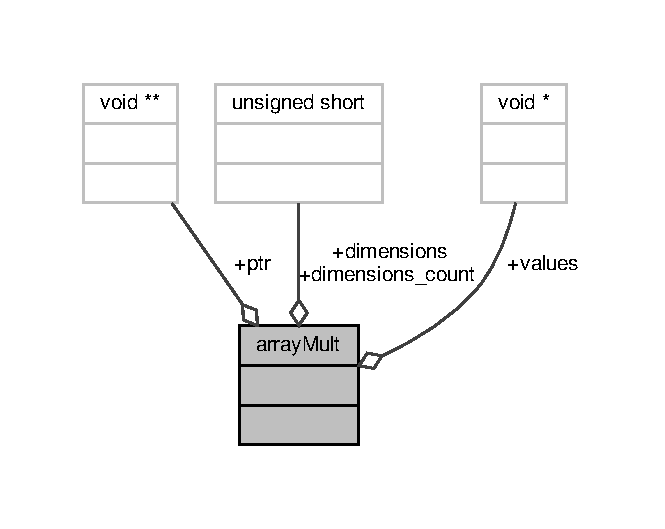
\includegraphics[width=319pt]{structarrayMult__coll__graph}
\end{center}
\end{figure}
\subsection*{Atributos Públicos}
\begin{DoxyCompactItemize}
\item 
\hyperlink{ClassLoader_8h_a5f223212eef04d10a4550ded680cb1cf}{u2} $\ast$ \hyperlink{structarrayMult_a32a40b7692ac520541539fe93367fb91}{dimensions}
\item 
\hyperlink{ClassLoader_8h_a5f223212eef04d10a4550ded680cb1cf}{u2} \hyperlink{structarrayMult_ad6c84cfce9d33584b955a601503867f1}{dimensions\+\_\+count}
\item 
void $\ast$$\ast$ \hyperlink{structarrayMult_a86583447f9a0c1c28284dd7f8476da24}{ptr}
\item 
void $\ast$ \hyperlink{structarrayMult_a5ed19e9ddbbc82d55d0800eca4ad4902}{values}
\end{DoxyCompactItemize}


\subsection{Descrição Detalhada}
Estrutura que gerencia os array multidimensionais. 

\subsection{Atributos}
\mbox{\Hypertarget{structarrayMult_a32a40b7692ac520541539fe93367fb91}\label{structarrayMult_a32a40b7692ac520541539fe93367fb91}} 
\index{array\+Mult@{array\+Mult}!dimensions@{dimensions}}
\index{dimensions@{dimensions}!array\+Mult@{array\+Mult}}
\subsubsection{\texorpdfstring{dimensions}{dimensions}}
{\footnotesize\ttfamily \hyperlink{ClassLoader_8h_a5f223212eef04d10a4550ded680cb1cf}{u2}$\ast$ array\+Mult\+::dimensions}

\mbox{\Hypertarget{structarrayMult_ad6c84cfce9d33584b955a601503867f1}\label{structarrayMult_ad6c84cfce9d33584b955a601503867f1}} 
\index{array\+Mult@{array\+Mult}!dimensions\+\_\+count@{dimensions\+\_\+count}}
\index{dimensions\+\_\+count@{dimensions\+\_\+count}!array\+Mult@{array\+Mult}}
\subsubsection{\texorpdfstring{dimensions\+\_\+count}{dimensions\_count}}
{\footnotesize\ttfamily \hyperlink{ClassLoader_8h_a5f223212eef04d10a4550ded680cb1cf}{u2} array\+Mult\+::dimensions\+\_\+count}

\mbox{\Hypertarget{structarrayMult_a86583447f9a0c1c28284dd7f8476da24}\label{structarrayMult_a86583447f9a0c1c28284dd7f8476da24}} 
\index{array\+Mult@{array\+Mult}!ptr@{ptr}}
\index{ptr@{ptr}!array\+Mult@{array\+Mult}}
\subsubsection{\texorpdfstring{ptr}{ptr}}
{\footnotesize\ttfamily void$\ast$$\ast$ array\+Mult\+::ptr}

\mbox{\Hypertarget{structarrayMult_a5ed19e9ddbbc82d55d0800eca4ad4902}\label{structarrayMult_a5ed19e9ddbbc82d55d0800eca4ad4902}} 
\index{array\+Mult@{array\+Mult}!values@{values}}
\index{values@{values}!array\+Mult@{array\+Mult}}
\subsubsection{\texorpdfstring{values}{values}}
{\footnotesize\ttfamily void$\ast$ array\+Mult\+::values}



A documentação para esta estrutura foi gerada a partir do seguinte arquivo\+:\begin{DoxyCompactItemize}
\item 
\hyperlink{MethodArea_8h}{Method\+Area.\+h}\end{DoxyCompactItemize}

\hypertarget{structattribute__info}{}\section{Referência da Estrutura attribute\+\_\+info}
\label{structattribute__info}\index{attribute\+\_\+info@{attribute\+\_\+info}}


Estrutura das informações dos atributos.  




{\ttfamily \#include $<$Class\+Loader.\+h$>$}



Diagrama de colaboração para attribute\+\_\+info\+:
\nopagebreak
\begin{figure}[H]
\begin{center}
\leavevmode
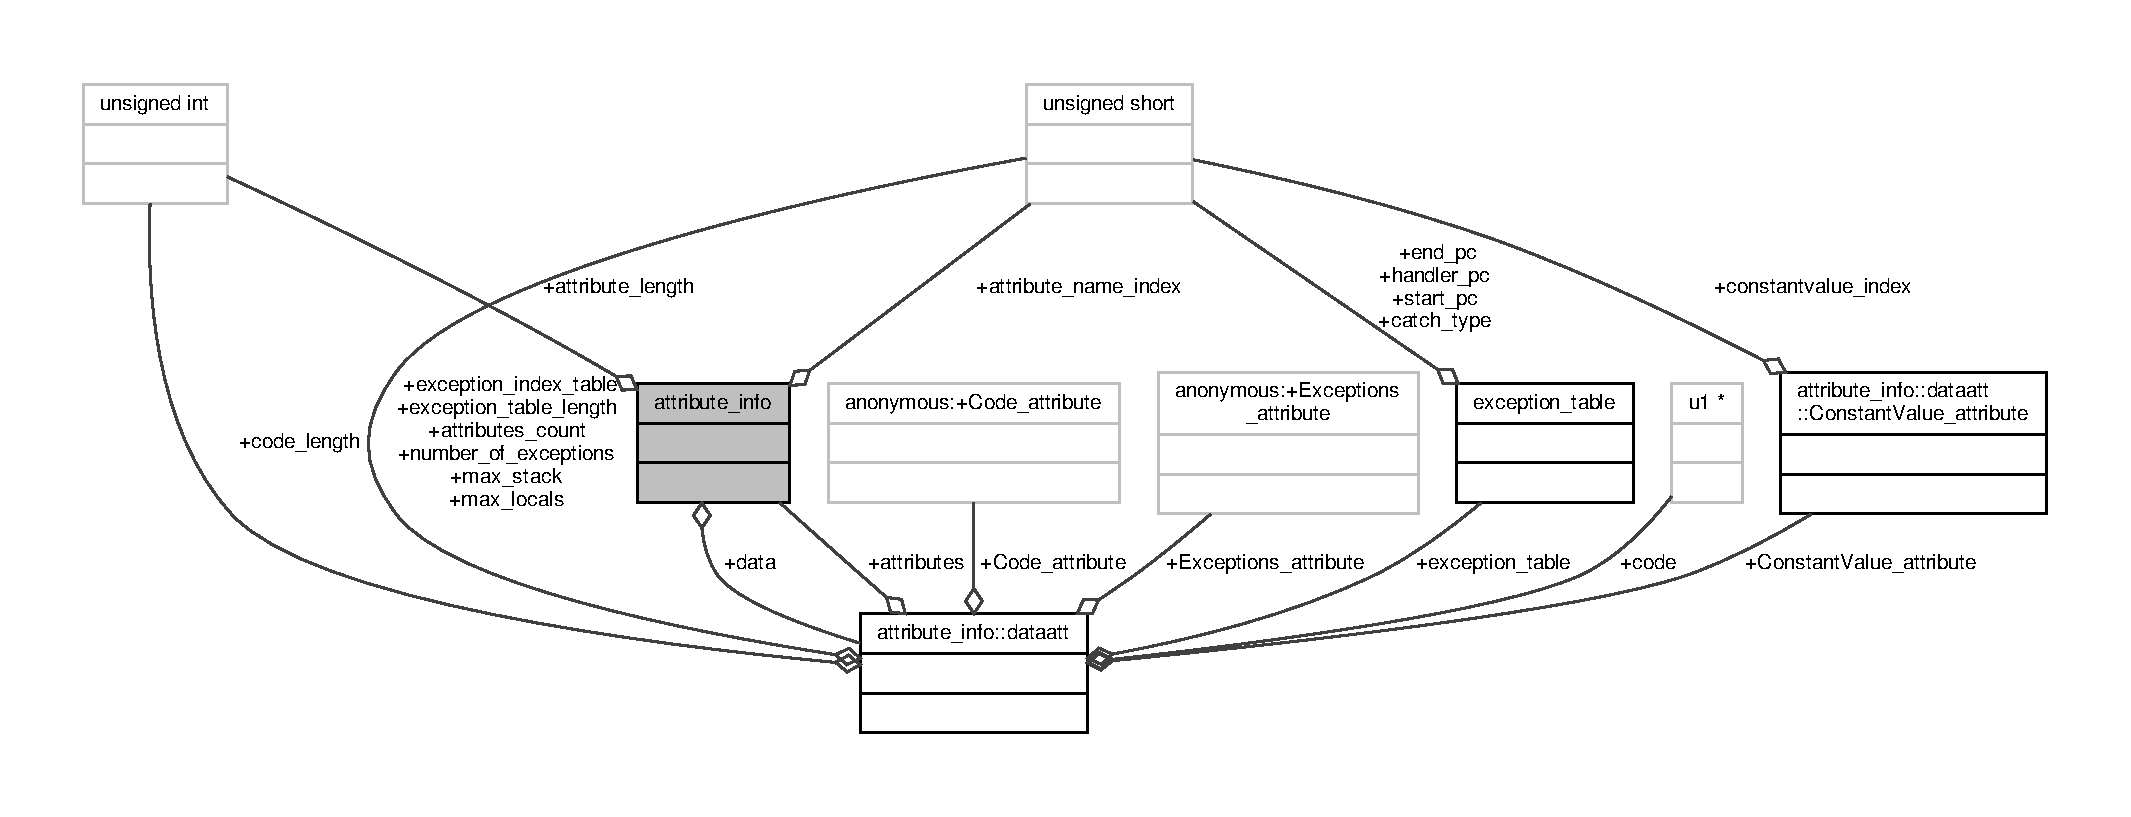
\includegraphics[width=350pt]{structattribute__info__coll__graph}
\end{center}
\end{figure}
\subsection*{Componentes}
\begin{DoxyCompactItemize}
\item 
union \hyperlink{unionattribute__info_1_1dataatt}{dataatt}
\end{DoxyCompactItemize}
\subsection*{Atributos Públicos}
\begin{DoxyCompactItemize}
\item 
\hyperlink{ClassLoader_8h_a5f223212eef04d10a4550ded680cb1cf}{u2} \hyperlink{structattribute__info_a19df9d4b42eb55ca5dc1bed98df89378}{attribute\+\_\+name\+\_\+index}
\item 
\hyperlink{ClassLoader_8h_aedf6ddc03df8caaaccbb4c60b9a9b850}{u4} \hyperlink{structattribute__info_a1ed8f679458c4bb0ed3315721588f50d}{attribute\+\_\+length}
\item 
union \hyperlink{unionattribute__info_1_1dataatt}{attribute\+\_\+info\+::dataatt} \hyperlink{structattribute__info_a63cd7230a276bdc8fc0d9eefc730c0db}{data}
\end{DoxyCompactItemize}


\subsection{Descrição Detalhada}
Estrutura das informações dos atributos. 

\subsection{Atributos}
\mbox{\Hypertarget{structattribute__info_a1ed8f679458c4bb0ed3315721588f50d}\label{structattribute__info_a1ed8f679458c4bb0ed3315721588f50d}} 
\index{attribute\+\_\+info@{attribute\+\_\+info}!attribute\+\_\+length@{attribute\+\_\+length}}
\index{attribute\+\_\+length@{attribute\+\_\+length}!attribute\+\_\+info@{attribute\+\_\+info}}
\subsubsection{\texorpdfstring{attribute\+\_\+length}{attribute\_length}}
{\footnotesize\ttfamily \hyperlink{ClassLoader_8h_aedf6ddc03df8caaaccbb4c60b9a9b850}{u4} attribute\+\_\+info\+::attribute\+\_\+length}

\mbox{\Hypertarget{structattribute__info_a19df9d4b42eb55ca5dc1bed98df89378}\label{structattribute__info_a19df9d4b42eb55ca5dc1bed98df89378}} 
\index{attribute\+\_\+info@{attribute\+\_\+info}!attribute\+\_\+name\+\_\+index@{attribute\+\_\+name\+\_\+index}}
\index{attribute\+\_\+name\+\_\+index@{attribute\+\_\+name\+\_\+index}!attribute\+\_\+info@{attribute\+\_\+info}}
\subsubsection{\texorpdfstring{attribute\+\_\+name\+\_\+index}{attribute\_name\_index}}
{\footnotesize\ttfamily \hyperlink{ClassLoader_8h_a5f223212eef04d10a4550ded680cb1cf}{u2} attribute\+\_\+info\+::attribute\+\_\+name\+\_\+index}

\mbox{\Hypertarget{structattribute__info_a63cd7230a276bdc8fc0d9eefc730c0db}\label{structattribute__info_a63cd7230a276bdc8fc0d9eefc730c0db}} 
\index{attribute\+\_\+info@{attribute\+\_\+info}!data@{data}}
\index{data@{data}!attribute\+\_\+info@{attribute\+\_\+info}}
\subsubsection{\texorpdfstring{data}{data}}
{\footnotesize\ttfamily union \hyperlink{unionattribute__info_1_1dataatt}{attribute\+\_\+info\+::dataatt} attribute\+\_\+info\+::data}



A documentação para esta estrutura foi gerada a partir do seguinte arquivo\+:\begin{DoxyCompactItemize}
\item 
\hyperlink{ClassLoader_8h}{Class\+Loader.\+h}\end{DoxyCompactItemize}

\hypertarget{structClass}{}\section{Referência da Estrutura Class}
\label{structClass}\index{Class@{Class}}


Estrutura que gerencia uma classe carregada.  




{\ttfamily \#include $<$Method\+Area.\+h$>$}



Diagrama de colaboração para Class\+:\nopagebreak
\begin{figure}[H]
\begin{center}
\leavevmode
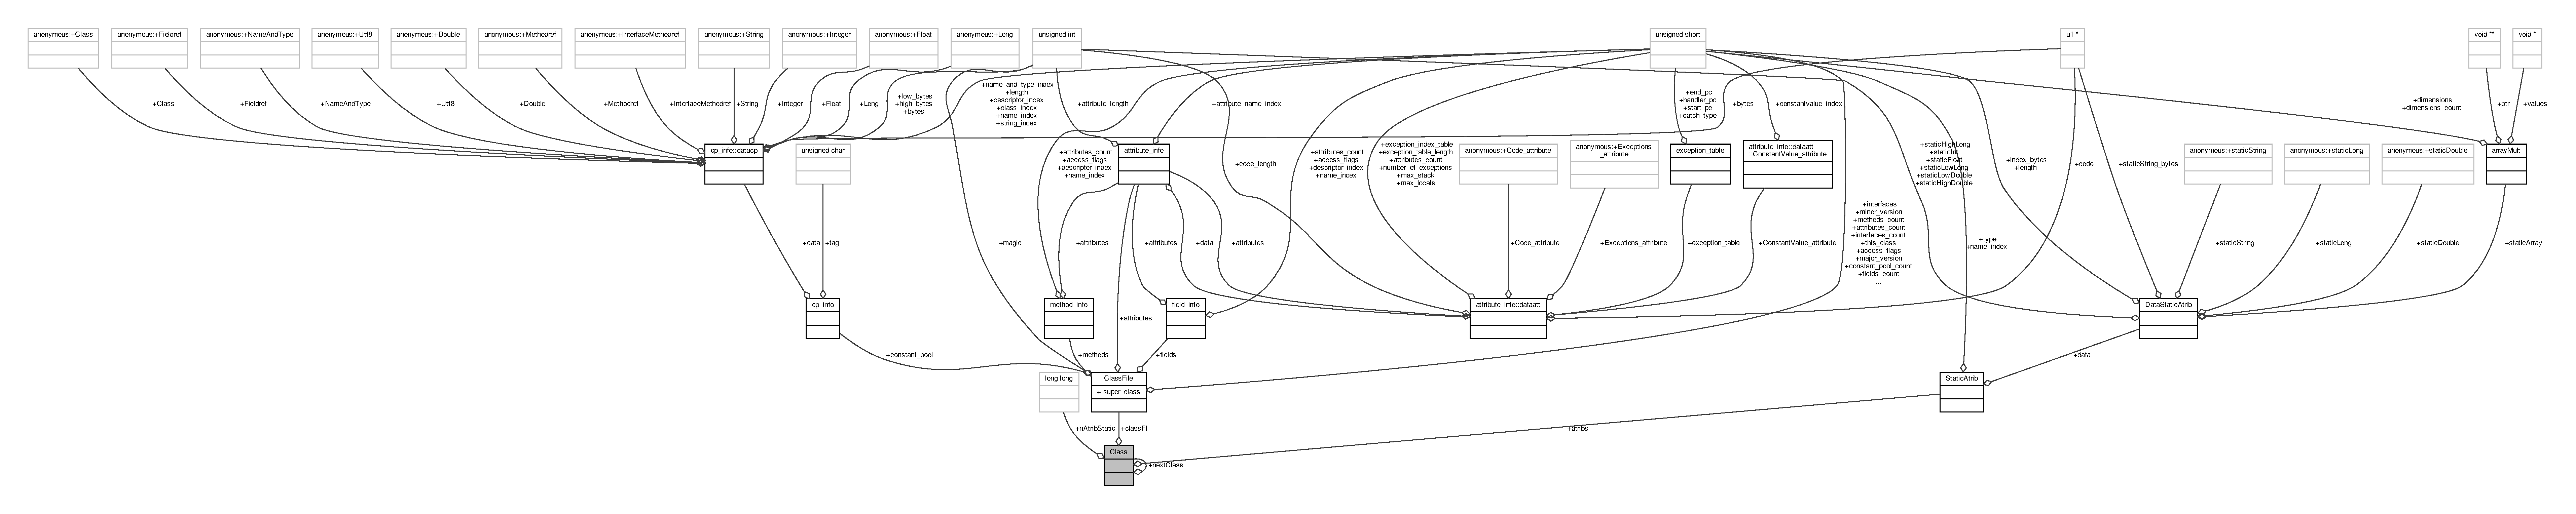
\includegraphics[width=350pt]{structClass__coll__graph}
\end{center}
\end{figure}
\subsection*{Atributos Públicos}
\begin{DoxyCompactItemize}
\item 
\hyperlink{structClassFile}{Class\+File} $\ast$ \hyperlink{structClass_a13dbcdd95b80b2c8fbd266a656ca927a}{class\+Fl}
\item 
long long \hyperlink{structClass_a8af3ca1a9103400ec8118948464edad0}{n\+Atrib\+Static}
\item 
\hyperlink{structStaticAtrib}{Static\+Atrib} $\ast$ \hyperlink{structClass_a6cf0307cc3e514a4e8c6afb54f050da8}{atribs}
\item 
struct \hyperlink{structClass}{Class} $\ast$ \hyperlink{structClass_a79ceca419d487e69bc791a3c2e1a96f2}{next\+Class}
\end{DoxyCompactItemize}


\subsection{Descrição Detalhada}
Estrutura que gerencia uma classe carregada. 

\subsection{Atributos}
\mbox{\Hypertarget{structClass_a6cf0307cc3e514a4e8c6afb54f050da8}\label{structClass_a6cf0307cc3e514a4e8c6afb54f050da8}} 
\index{Class@{Class}!atribs@{atribs}}
\index{atribs@{atribs}!Class@{Class}}
\subsubsection{\texorpdfstring{atribs}{atribs}}
{\footnotesize\ttfamily \hyperlink{structStaticAtrib}{Static\+Atrib}$\ast$ Class\+::atribs}

\mbox{\Hypertarget{structClass_a13dbcdd95b80b2c8fbd266a656ca927a}\label{structClass_a13dbcdd95b80b2c8fbd266a656ca927a}} 
\index{Class@{Class}!class\+Fl@{class\+Fl}}
\index{class\+Fl@{class\+Fl}!Class@{Class}}
\subsubsection{\texorpdfstring{class\+Fl}{classFl}}
{\footnotesize\ttfamily \hyperlink{structClassFile}{Class\+File}$\ast$ Class\+::class\+Fl}

\mbox{\Hypertarget{structClass_a8af3ca1a9103400ec8118948464edad0}\label{structClass_a8af3ca1a9103400ec8118948464edad0}} 
\index{Class@{Class}!n\+Atrib\+Static@{n\+Atrib\+Static}}
\index{n\+Atrib\+Static@{n\+Atrib\+Static}!Class@{Class}}
\subsubsection{\texorpdfstring{n\+Atrib\+Static}{nAtribStatic}}
{\footnotesize\ttfamily long long Class\+::n\+Atrib\+Static}

\mbox{\Hypertarget{structClass_a79ceca419d487e69bc791a3c2e1a96f2}\label{structClass_a79ceca419d487e69bc791a3c2e1a96f2}} 
\index{Class@{Class}!next\+Class@{next\+Class}}
\index{next\+Class@{next\+Class}!Class@{Class}}
\subsubsection{\texorpdfstring{next\+Class}{nextClass}}
{\footnotesize\ttfamily struct \hyperlink{structClass}{Class}$\ast$ Class\+::next\+Class}



A documentação para esta estrutura foi gerada a partir do seguinte arquivo\+:\begin{DoxyCompactItemize}
\item 
\hyperlink{MethodArea_8h}{Method\+Area.\+h}\end{DoxyCompactItemize}

\hypertarget{structClassFile}{}\section{Referência da Estrutura Class\+File}
\label{structClassFile}\index{Class\+File@{Class\+File}}


Escrutura da classe.  




{\ttfamily \#include $<$Class\+Loader.\+h$>$}



Diagrama de colaboração para Class\+File\+:\nopagebreak
\begin{figure}[H]
\begin{center}
\leavevmode
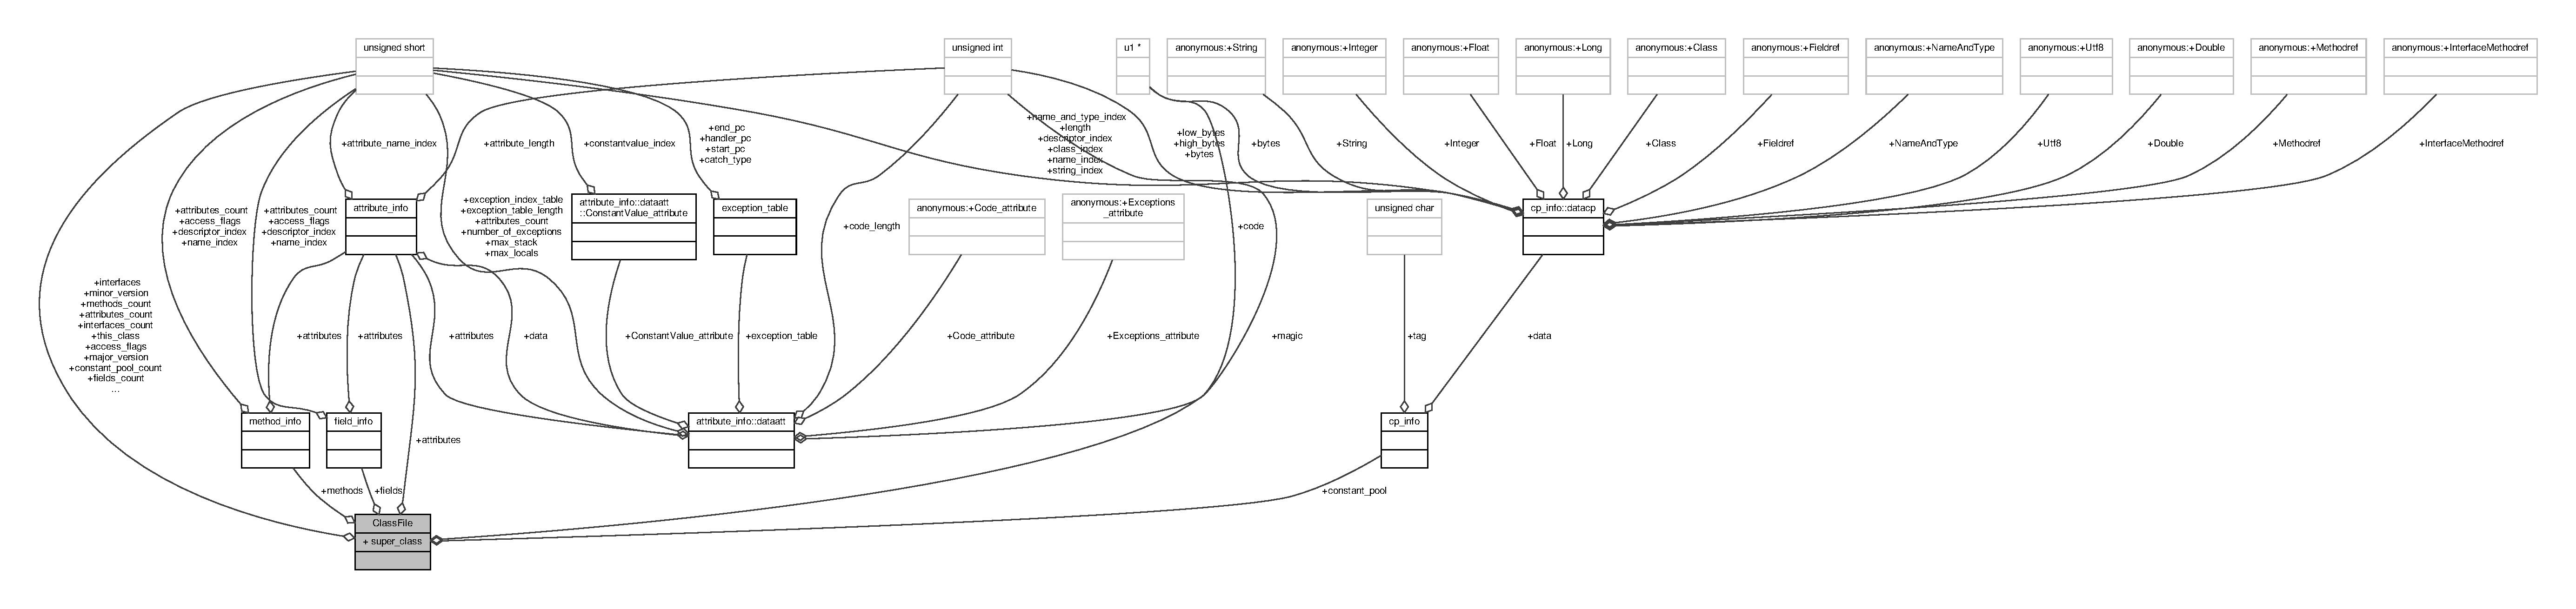
\includegraphics[width=350pt]{structClassFile__coll__graph}
\end{center}
\end{figure}
\subsection*{Atributos Públicos}
\begin{DoxyCompactItemize}
\item 
\hyperlink{ClassLoader_8h_aedf6ddc03df8caaaccbb4c60b9a9b850}{u4} \hyperlink{structClassFile_a09085e9db513dae2f46da6e0a26c1b59}{magic}
\item 
\hyperlink{ClassLoader_8h_a5f223212eef04d10a4550ded680cb1cf}{u2} \hyperlink{structClassFile_af0db7b0ea01cb9cea2cee177ca81df09}{minor\+\_\+version}
\item 
\hyperlink{ClassLoader_8h_a5f223212eef04d10a4550ded680cb1cf}{u2} \hyperlink{structClassFile_abede9cb937e65072517d0ee6e26e2757}{major\+\_\+version}
\item 
\hyperlink{ClassLoader_8h_a5f223212eef04d10a4550ded680cb1cf}{u2} \hyperlink{structClassFile_ac8fdf5cccfd632da4fdb21ae63fffa7a}{constant\+\_\+pool\+\_\+count}
\item 
\hyperlink{structcp__info}{cp\+\_\+info} $\ast$ \hyperlink{structClassFile_a2309d843091aad79aed04ce92470a434}{constant\+\_\+pool}
\item 
\hyperlink{ClassLoader_8h_a5f223212eef04d10a4550ded680cb1cf}{u2} \hyperlink{structClassFile_ae88db578147f7ee0d6fc1aeacb341854}{access\+\_\+flags}
\item 
\hyperlink{ClassLoader_8h_a5f223212eef04d10a4550ded680cb1cf}{u2} \hyperlink{structClassFile_a2d33db0a560a71b94bc572dd1e4ec03a}{this\+\_\+class}
\item 
\hyperlink{ClassLoader_8h_a5f223212eef04d10a4550ded680cb1cf}{u2} \hyperlink{structClassFile_a5f6c11c0ccb02fd992b5c102725253ec}{super\+\_\+class}
\item 
\hyperlink{ClassLoader_8h_a5f223212eef04d10a4550ded680cb1cf}{u2} \hyperlink{structClassFile_a337fcb7da33d1b64631441115c7de305}{interfaces\+\_\+count}
\item 
\hyperlink{ClassLoader_8h_a5f223212eef04d10a4550ded680cb1cf}{u2} $\ast$ \hyperlink{structClassFile_af599de97e062c98966470f1590496425}{interfaces}
\item 
\hyperlink{ClassLoader_8h_a5f223212eef04d10a4550ded680cb1cf}{u2} \hyperlink{structClassFile_acea207ee523fbc16611d3cf436c390e0}{fields\+\_\+count}
\item 
\hyperlink{structfield__info}{field\+\_\+info} $\ast$ \hyperlink{structClassFile_aa324f88c75aa96c632f8c57d010aab0c}{fields}
\item 
\hyperlink{ClassLoader_8h_a5f223212eef04d10a4550ded680cb1cf}{u2} \hyperlink{structClassFile_aacfb45d4af64216324b1ae5269c870d5}{methods\+\_\+count}
\item 
\hyperlink{structmethod__info}{method\+\_\+info} $\ast$ \hyperlink{structClassFile_ad061f06cd709d10dbfbf82f443e43632}{methods}
\item 
\hyperlink{ClassLoader_8h_a5f223212eef04d10a4550ded680cb1cf}{u2} \hyperlink{structClassFile_a633c696fbe08e7e7906b2ab1e52f3d1b}{attributes\+\_\+count}
\item 
\hyperlink{structattribute__info}{attribute\+\_\+info} $\ast$ \hyperlink{structClassFile_a8bf809db8e1008f401dc3cda5e9cdb14}{attributes}
\end{DoxyCompactItemize}


\subsection{Descrição Detalhada}
Escrutura da classe. 

\subsection{Atributos}
\mbox{\Hypertarget{structClassFile_ae88db578147f7ee0d6fc1aeacb341854}\label{structClassFile_ae88db578147f7ee0d6fc1aeacb341854}} 
\index{Class\+File@{Class\+File}!access\+\_\+flags@{access\+\_\+flags}}
\index{access\+\_\+flags@{access\+\_\+flags}!Class\+File@{Class\+File}}
\subsubsection{\texorpdfstring{access\+\_\+flags}{access\_flags}}
{\footnotesize\ttfamily \hyperlink{ClassLoader_8h_a5f223212eef04d10a4550ded680cb1cf}{u2} Class\+File\+::access\+\_\+flags}

\mbox{\Hypertarget{structClassFile_a8bf809db8e1008f401dc3cda5e9cdb14}\label{structClassFile_a8bf809db8e1008f401dc3cda5e9cdb14}} 
\index{Class\+File@{Class\+File}!attributes@{attributes}}
\index{attributes@{attributes}!Class\+File@{Class\+File}}
\subsubsection{\texorpdfstring{attributes}{attributes}}
{\footnotesize\ttfamily \hyperlink{structattribute__info}{attribute\+\_\+info}$\ast$ Class\+File\+::attributes}

\mbox{\Hypertarget{structClassFile_a633c696fbe08e7e7906b2ab1e52f3d1b}\label{structClassFile_a633c696fbe08e7e7906b2ab1e52f3d1b}} 
\index{Class\+File@{Class\+File}!attributes\+\_\+count@{attributes\+\_\+count}}
\index{attributes\+\_\+count@{attributes\+\_\+count}!Class\+File@{Class\+File}}
\subsubsection{\texorpdfstring{attributes\+\_\+count}{attributes\_count}}
{\footnotesize\ttfamily \hyperlink{ClassLoader_8h_a5f223212eef04d10a4550ded680cb1cf}{u2} Class\+File\+::attributes\+\_\+count}

\mbox{\Hypertarget{structClassFile_a2309d843091aad79aed04ce92470a434}\label{structClassFile_a2309d843091aad79aed04ce92470a434}} 
\index{Class\+File@{Class\+File}!constant\+\_\+pool@{constant\+\_\+pool}}
\index{constant\+\_\+pool@{constant\+\_\+pool}!Class\+File@{Class\+File}}
\subsubsection{\texorpdfstring{constant\+\_\+pool}{constant\_pool}}
{\footnotesize\ttfamily \hyperlink{structcp__info}{cp\+\_\+info}$\ast$ Class\+File\+::constant\+\_\+pool}

\mbox{\Hypertarget{structClassFile_ac8fdf5cccfd632da4fdb21ae63fffa7a}\label{structClassFile_ac8fdf5cccfd632da4fdb21ae63fffa7a}} 
\index{Class\+File@{Class\+File}!constant\+\_\+pool\+\_\+count@{constant\+\_\+pool\+\_\+count}}
\index{constant\+\_\+pool\+\_\+count@{constant\+\_\+pool\+\_\+count}!Class\+File@{Class\+File}}
\subsubsection{\texorpdfstring{constant\+\_\+pool\+\_\+count}{constant\_pool\_count}}
{\footnotesize\ttfamily \hyperlink{ClassLoader_8h_a5f223212eef04d10a4550ded680cb1cf}{u2} Class\+File\+::constant\+\_\+pool\+\_\+count}

\mbox{\Hypertarget{structClassFile_aa324f88c75aa96c632f8c57d010aab0c}\label{structClassFile_aa324f88c75aa96c632f8c57d010aab0c}} 
\index{Class\+File@{Class\+File}!fields@{fields}}
\index{fields@{fields}!Class\+File@{Class\+File}}
\subsubsection{\texorpdfstring{fields}{fields}}
{\footnotesize\ttfamily \hyperlink{structfield__info}{field\+\_\+info}$\ast$ Class\+File\+::fields}

\mbox{\Hypertarget{structClassFile_acea207ee523fbc16611d3cf436c390e0}\label{structClassFile_acea207ee523fbc16611d3cf436c390e0}} 
\index{Class\+File@{Class\+File}!fields\+\_\+count@{fields\+\_\+count}}
\index{fields\+\_\+count@{fields\+\_\+count}!Class\+File@{Class\+File}}
\subsubsection{\texorpdfstring{fields\+\_\+count}{fields\_count}}
{\footnotesize\ttfamily \hyperlink{ClassLoader_8h_a5f223212eef04d10a4550ded680cb1cf}{u2} Class\+File\+::fields\+\_\+count}

\mbox{\Hypertarget{structClassFile_af599de97e062c98966470f1590496425}\label{structClassFile_af599de97e062c98966470f1590496425}} 
\index{Class\+File@{Class\+File}!interfaces@{interfaces}}
\index{interfaces@{interfaces}!Class\+File@{Class\+File}}
\subsubsection{\texorpdfstring{interfaces}{interfaces}}
{\footnotesize\ttfamily \hyperlink{ClassLoader_8h_a5f223212eef04d10a4550ded680cb1cf}{u2}$\ast$ Class\+File\+::interfaces}

\mbox{\Hypertarget{structClassFile_a337fcb7da33d1b64631441115c7de305}\label{structClassFile_a337fcb7da33d1b64631441115c7de305}} 
\index{Class\+File@{Class\+File}!interfaces\+\_\+count@{interfaces\+\_\+count}}
\index{interfaces\+\_\+count@{interfaces\+\_\+count}!Class\+File@{Class\+File}}
\subsubsection{\texorpdfstring{interfaces\+\_\+count}{interfaces\_count}}
{\footnotesize\ttfamily \hyperlink{ClassLoader_8h_a5f223212eef04d10a4550ded680cb1cf}{u2} Class\+File\+::interfaces\+\_\+count}

\mbox{\Hypertarget{structClassFile_a09085e9db513dae2f46da6e0a26c1b59}\label{structClassFile_a09085e9db513dae2f46da6e0a26c1b59}} 
\index{Class\+File@{Class\+File}!magic@{magic}}
\index{magic@{magic}!Class\+File@{Class\+File}}
\subsubsection{\texorpdfstring{magic}{magic}}
{\footnotesize\ttfamily \hyperlink{ClassLoader_8h_aedf6ddc03df8caaaccbb4c60b9a9b850}{u4} Class\+File\+::magic}

\mbox{\Hypertarget{structClassFile_abede9cb937e65072517d0ee6e26e2757}\label{structClassFile_abede9cb937e65072517d0ee6e26e2757}} 
\index{Class\+File@{Class\+File}!major\+\_\+version@{major\+\_\+version}}
\index{major\+\_\+version@{major\+\_\+version}!Class\+File@{Class\+File}}
\subsubsection{\texorpdfstring{major\+\_\+version}{major\_version}}
{\footnotesize\ttfamily \hyperlink{ClassLoader_8h_a5f223212eef04d10a4550ded680cb1cf}{u2} Class\+File\+::major\+\_\+version}

\mbox{\Hypertarget{structClassFile_ad061f06cd709d10dbfbf82f443e43632}\label{structClassFile_ad061f06cd709d10dbfbf82f443e43632}} 
\index{Class\+File@{Class\+File}!methods@{methods}}
\index{methods@{methods}!Class\+File@{Class\+File}}
\subsubsection{\texorpdfstring{methods}{methods}}
{\footnotesize\ttfamily \hyperlink{structmethod__info}{method\+\_\+info}$\ast$ Class\+File\+::methods}

\mbox{\Hypertarget{structClassFile_aacfb45d4af64216324b1ae5269c870d5}\label{structClassFile_aacfb45d4af64216324b1ae5269c870d5}} 
\index{Class\+File@{Class\+File}!methods\+\_\+count@{methods\+\_\+count}}
\index{methods\+\_\+count@{methods\+\_\+count}!Class\+File@{Class\+File}}
\subsubsection{\texorpdfstring{methods\+\_\+count}{methods\_count}}
{\footnotesize\ttfamily \hyperlink{ClassLoader_8h_a5f223212eef04d10a4550ded680cb1cf}{u2} Class\+File\+::methods\+\_\+count}

\mbox{\Hypertarget{structClassFile_af0db7b0ea01cb9cea2cee177ca81df09}\label{structClassFile_af0db7b0ea01cb9cea2cee177ca81df09}} 
\index{Class\+File@{Class\+File}!minor\+\_\+version@{minor\+\_\+version}}
\index{minor\+\_\+version@{minor\+\_\+version}!Class\+File@{Class\+File}}
\subsubsection{\texorpdfstring{minor\+\_\+version}{minor\_version}}
{\footnotesize\ttfamily \hyperlink{ClassLoader_8h_a5f223212eef04d10a4550ded680cb1cf}{u2} Class\+File\+::minor\+\_\+version}

\mbox{\Hypertarget{structClassFile_a5f6c11c0ccb02fd992b5c102725253ec}\label{structClassFile_a5f6c11c0ccb02fd992b5c102725253ec}} 
\index{Class\+File@{Class\+File}!super\+\_\+class@{super\+\_\+class}}
\index{super\+\_\+class@{super\+\_\+class}!Class\+File@{Class\+File}}
\subsubsection{\texorpdfstring{super\+\_\+class}{super\_class}}
{\footnotesize\ttfamily \hyperlink{ClassLoader_8h_a5f223212eef04d10a4550ded680cb1cf}{u2} Class\+File\+::super\+\_\+class}

\mbox{\Hypertarget{structClassFile_a2d33db0a560a71b94bc572dd1e4ec03a}\label{structClassFile_a2d33db0a560a71b94bc572dd1e4ec03a}} 
\index{Class\+File@{Class\+File}!this\+\_\+class@{this\+\_\+class}}
\index{this\+\_\+class@{this\+\_\+class}!Class\+File@{Class\+File}}
\subsubsection{\texorpdfstring{this\+\_\+class}{this\_class}}
{\footnotesize\ttfamily \hyperlink{ClassLoader_8h_a5f223212eef04d10a4550ded680cb1cf}{u2} Class\+File\+::this\+\_\+class}



A documentação para esta estrutura foi gerada a partir do seguinte arquivo\+:\begin{DoxyCompactItemize}
\item 
\hyperlink{ClassLoader_8h}{Class\+Loader.\+h}\end{DoxyCompactItemize}

\hypertarget{structclasstype__info}{}\section{Referência da Estrutura classtype\+\_\+info}
\label{structclasstype__info}\index{classtype\+\_\+info@{classtype\+\_\+info}}


{\ttfamily \#include $<$Class\+Loader.\+h$>$}



Diagrama de colaboração para classtype\+\_\+info\+:
\nopagebreak
\begin{figure}[H]
\begin{center}
\leavevmode
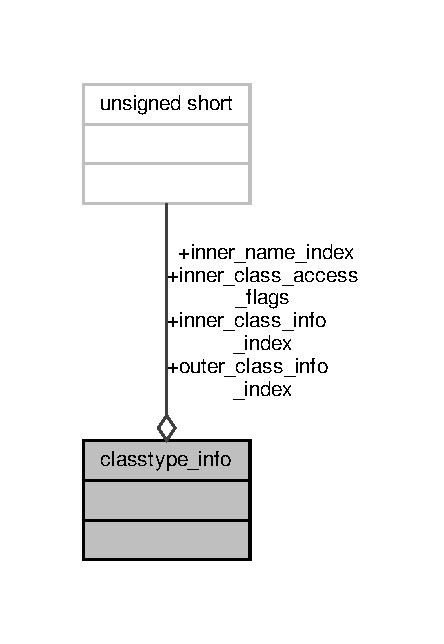
\includegraphics[width=213pt]{structclasstype__info__coll__graph}
\end{center}
\end{figure}
\subsection*{Atributos Públicos}
\begin{DoxyCompactItemize}
\item 
\hyperlink{ClassLoader_8h_a5f223212eef04d10a4550ded680cb1cf}{u2} \hyperlink{structclasstype__info_a3d095ea8d63dca94b9feb3a365b1f52e}{inner\+\_\+class\+\_\+info\+\_\+index}
\item 
\hyperlink{ClassLoader_8h_a5f223212eef04d10a4550ded680cb1cf}{u2} \hyperlink{structclasstype__info_addb19ba72e3ccfc7b7e5630b872e87f1}{outer\+\_\+class\+\_\+info\+\_\+index}
\item 
\hyperlink{ClassLoader_8h_a5f223212eef04d10a4550ded680cb1cf}{u2} \hyperlink{structclasstype__info_a55194f64ad8da0051fd2457811852eda}{inner\+\_\+name\+\_\+index}
\item 
\hyperlink{ClassLoader_8h_a5f223212eef04d10a4550ded680cb1cf}{u2} \hyperlink{structclasstype__info_a2e4834ba45e2650aa080837472e9afc4}{inner\+\_\+class\+\_\+access\+\_\+flags}
\end{DoxyCompactItemize}


\subsection{Atributos}
\mbox{\Hypertarget{structclasstype__info_a2e4834ba45e2650aa080837472e9afc4}\label{structclasstype__info_a2e4834ba45e2650aa080837472e9afc4}} 
\index{classtype\+\_\+info@{classtype\+\_\+info}!inner\+\_\+class\+\_\+access\+\_\+flags@{inner\+\_\+class\+\_\+access\+\_\+flags}}
\index{inner\+\_\+class\+\_\+access\+\_\+flags@{inner\+\_\+class\+\_\+access\+\_\+flags}!classtype\+\_\+info@{classtype\+\_\+info}}
\subsubsection{\texorpdfstring{inner\+\_\+class\+\_\+access\+\_\+flags}{inner\_class\_access\_flags}}
{\footnotesize\ttfamily \hyperlink{ClassLoader_8h_a5f223212eef04d10a4550ded680cb1cf}{u2} classtype\+\_\+info\+::inner\+\_\+class\+\_\+access\+\_\+flags}

\mbox{\Hypertarget{structclasstype__info_a3d095ea8d63dca94b9feb3a365b1f52e}\label{structclasstype__info_a3d095ea8d63dca94b9feb3a365b1f52e}} 
\index{classtype\+\_\+info@{classtype\+\_\+info}!inner\+\_\+class\+\_\+info\+\_\+index@{inner\+\_\+class\+\_\+info\+\_\+index}}
\index{inner\+\_\+class\+\_\+info\+\_\+index@{inner\+\_\+class\+\_\+info\+\_\+index}!classtype\+\_\+info@{classtype\+\_\+info}}
\subsubsection{\texorpdfstring{inner\+\_\+class\+\_\+info\+\_\+index}{inner\_class\_info\_index}}
{\footnotesize\ttfamily \hyperlink{ClassLoader_8h_a5f223212eef04d10a4550ded680cb1cf}{u2} classtype\+\_\+info\+::inner\+\_\+class\+\_\+info\+\_\+index}

\mbox{\Hypertarget{structclasstype__info_a55194f64ad8da0051fd2457811852eda}\label{structclasstype__info_a55194f64ad8da0051fd2457811852eda}} 
\index{classtype\+\_\+info@{classtype\+\_\+info}!inner\+\_\+name\+\_\+index@{inner\+\_\+name\+\_\+index}}
\index{inner\+\_\+name\+\_\+index@{inner\+\_\+name\+\_\+index}!classtype\+\_\+info@{classtype\+\_\+info}}
\subsubsection{\texorpdfstring{inner\+\_\+name\+\_\+index}{inner\_name\_index}}
{\footnotesize\ttfamily \hyperlink{ClassLoader_8h_a5f223212eef04d10a4550ded680cb1cf}{u2} classtype\+\_\+info\+::inner\+\_\+name\+\_\+index}

\mbox{\Hypertarget{structclasstype__info_addb19ba72e3ccfc7b7e5630b872e87f1}\label{structclasstype__info_addb19ba72e3ccfc7b7e5630b872e87f1}} 
\index{classtype\+\_\+info@{classtype\+\_\+info}!outer\+\_\+class\+\_\+info\+\_\+index@{outer\+\_\+class\+\_\+info\+\_\+index}}
\index{outer\+\_\+class\+\_\+info\+\_\+index@{outer\+\_\+class\+\_\+info\+\_\+index}!classtype\+\_\+info@{classtype\+\_\+info}}
\subsubsection{\texorpdfstring{outer\+\_\+class\+\_\+info\+\_\+index}{outer\_class\_info\_index}}
{\footnotesize\ttfamily \hyperlink{ClassLoader_8h_a5f223212eef04d10a4550ded680cb1cf}{u2} classtype\+\_\+info\+::outer\+\_\+class\+\_\+info\+\_\+index}



A documentação para esta estrutura foi gerada a partir do seguinte arquivo\+:\begin{DoxyCompactItemize}
\item 
\hyperlink{ClassLoader_8h}{Class\+Loader.\+h}\end{DoxyCompactItemize}

\hypertarget{structattribute__info_1_1dataatt_1_1ConstantValue__attribute}{}\section{Referência da Estrutura attribute\+\_\+info\+:\+:dataatt\+:\+:Constant\+Value\+\_\+attribute}
\label{structattribute__info_1_1dataatt_1_1ConstantValue__attribute}\index{attribute\+\_\+info\+::dataatt\+::\+Constant\+Value\+\_\+attribute@{attribute\+\_\+info\+::dataatt\+::\+Constant\+Value\+\_\+attribute}}


{\ttfamily \#include $<$Class\+Loader.\+h$>$}



Diagrama de colaboração para attribute\+\_\+info\+:\+:dataatt\+:\+:Constant\+Value\+\_\+attribute\+:\nopagebreak
\begin{figure}[H]
\begin{center}
\leavevmode
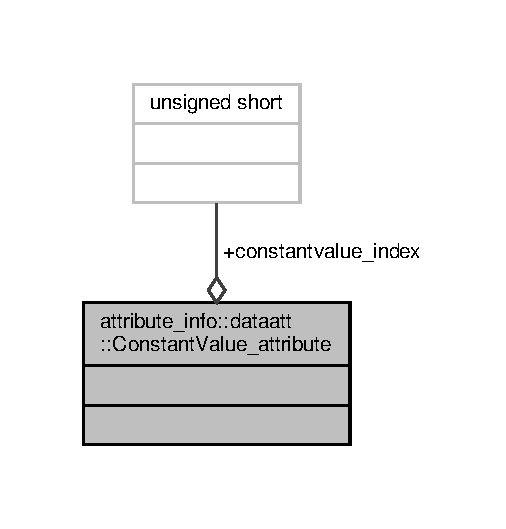
\includegraphics[width=243pt]{structattribute__info_1_1dataatt_1_1ConstantValue__attribute__coll__graph}
\end{center}
\end{figure}
\subsection*{Atributos Públicos}
\begin{DoxyCompactItemize}
\item 
\hyperlink{ClassLoader_8h_a5f223212eef04d10a4550ded680cb1cf}{u2} \hyperlink{structattribute__info_1_1dataatt_1_1ConstantValue__attribute_ac3d5541cf499281fbc9718155cf048fe}{constantvalue\+\_\+index}
\end{DoxyCompactItemize}


\subsection{Atributos}
\mbox{\Hypertarget{structattribute__info_1_1dataatt_1_1ConstantValue__attribute_ac3d5541cf499281fbc9718155cf048fe}\label{structattribute__info_1_1dataatt_1_1ConstantValue__attribute_ac3d5541cf499281fbc9718155cf048fe}} 
\index{attribute\+\_\+info\+::dataatt\+::\+Constant\+Value\+\_\+attribute@{attribute\+\_\+info\+::dataatt\+::\+Constant\+Value\+\_\+attribute}!constantvalue\+\_\+index@{constantvalue\+\_\+index}}
\index{constantvalue\+\_\+index@{constantvalue\+\_\+index}!attribute\+\_\+info\+::dataatt\+::\+Constant\+Value\+\_\+attribute@{attribute\+\_\+info\+::dataatt\+::\+Constant\+Value\+\_\+attribute}}
\subsubsection{\texorpdfstring{constantvalue\+\_\+index}{constantvalue\_index}}
{\footnotesize\ttfamily \hyperlink{ClassLoader_8h_a5f223212eef04d10a4550ded680cb1cf}{u2} attribute\+\_\+info\+::dataatt\+::\+Constant\+Value\+\_\+attribute\+::constantvalue\+\_\+index}



A documentação para esta estrutura foi gerada a partir do seguinte arquivo\+:\begin{DoxyCompactItemize}
\item 
\hyperlink{ClassLoader_8h}{Class\+Loader.\+h}\end{DoxyCompactItemize}

\hypertarget{structcp__info}{}\section{Referência da Estrutura cp\+\_\+info}
\label{structcp__info}\index{cp\+\_\+info@{cp\+\_\+info}}


Estrutura do constant pool.  




{\ttfamily \#include $<$Class\+Loader.\+h$>$}



Diagrama de colaboração para cp\+\_\+info\+:
\nopagebreak
\begin{figure}[H]
\begin{center}
\leavevmode
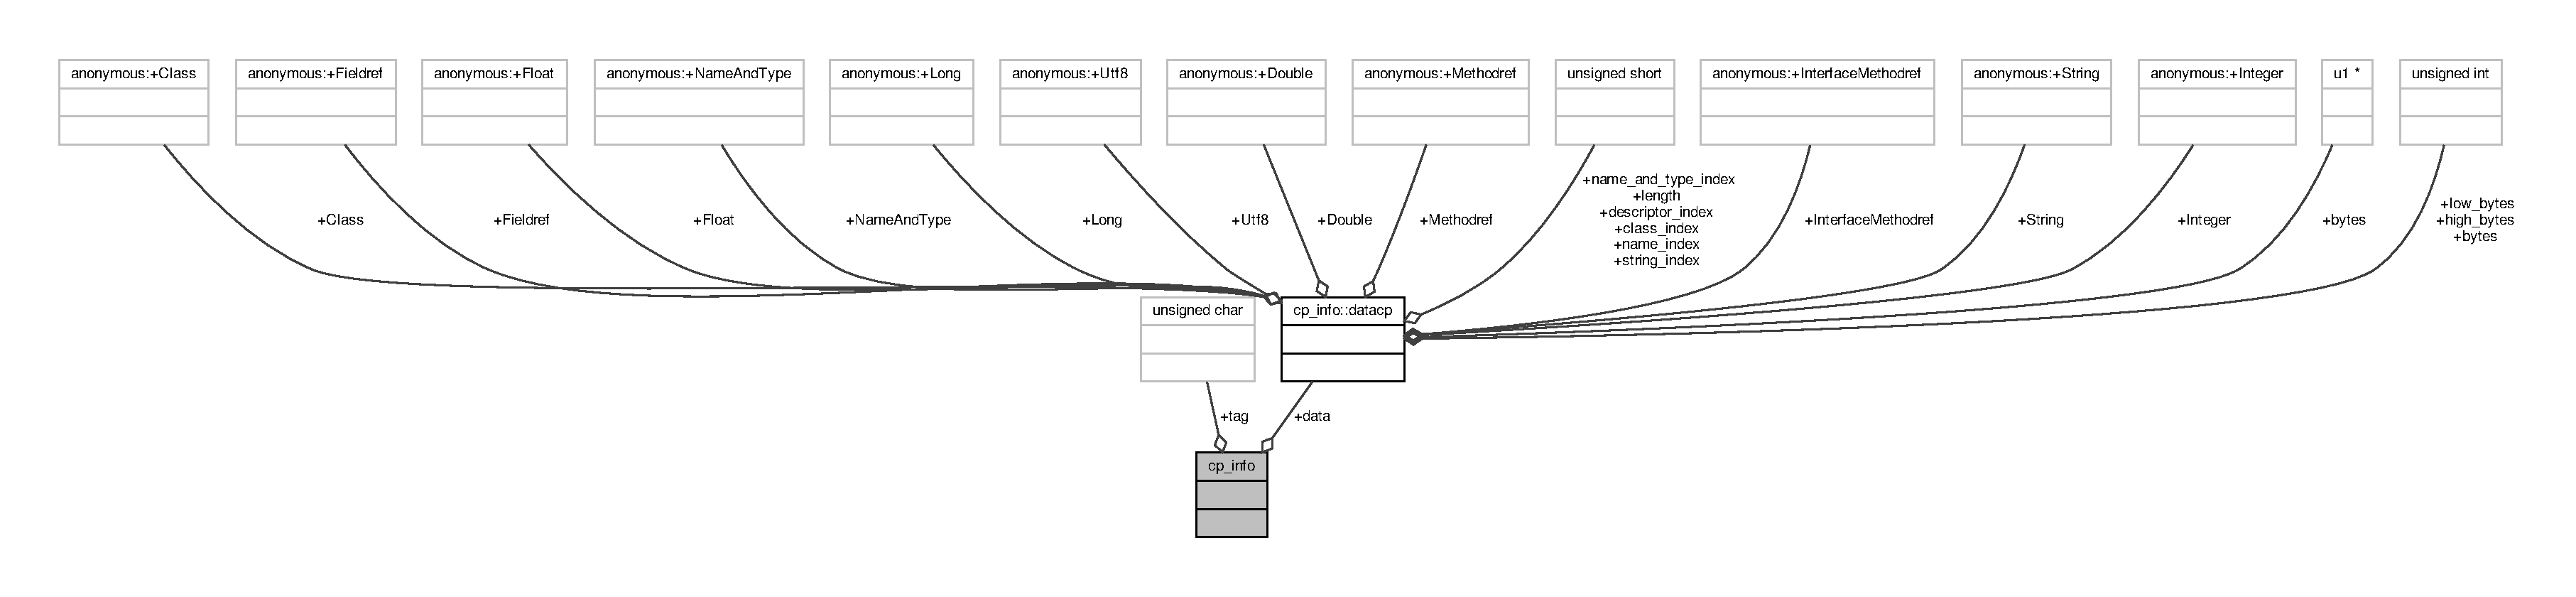
\includegraphics[width=350pt]{structcp__info__coll__graph}
\end{center}
\end{figure}
\subsection*{Componentes}
\begin{DoxyCompactItemize}
\item 
union \hyperlink{unioncp__info_1_1datacp}{datacp}
\end{DoxyCompactItemize}
\subsection*{Atributos Públicos}
\begin{DoxyCompactItemize}
\item 
\hyperlink{ClassLoader_8h_a216a9f8b04b4f0af84a4ca9d1d85a6ca}{u1} \hyperlink{structcp__info_a045b8801a6e96a2a31d3b62ea684f141}{tag}
\item 
union \hyperlink{unioncp__info_1_1datacp}{cp\+\_\+info\+::datacp} \hyperlink{structcp__info_a1c63f47410d9a935cfe2ce56075957cb}{data}
\end{DoxyCompactItemize}


\subsection{Descrição Detalhada}
Estrutura do constant pool. 

\subsection{Atributos}
\mbox{\Hypertarget{structcp__info_a1c63f47410d9a935cfe2ce56075957cb}\label{structcp__info_a1c63f47410d9a935cfe2ce56075957cb}} 
\index{cp\+\_\+info@{cp\+\_\+info}!data@{data}}
\index{data@{data}!cp\+\_\+info@{cp\+\_\+info}}
\subsubsection{\texorpdfstring{data}{data}}
{\footnotesize\ttfamily union \hyperlink{unioncp__info_1_1datacp}{cp\+\_\+info\+::datacp} cp\+\_\+info\+::data}

\mbox{\Hypertarget{structcp__info_a045b8801a6e96a2a31d3b62ea684f141}\label{structcp__info_a045b8801a6e96a2a31d3b62ea684f141}} 
\index{cp\+\_\+info@{cp\+\_\+info}!tag@{tag}}
\index{tag@{tag}!cp\+\_\+info@{cp\+\_\+info}}
\subsubsection{\texorpdfstring{tag}{tag}}
{\footnotesize\ttfamily \hyperlink{ClassLoader_8h_a216a9f8b04b4f0af84a4ca9d1d85a6ca}{u1} cp\+\_\+info\+::tag}



A documentação para esta estrutura foi gerada a partir do seguinte arquivo\+:\begin{DoxyCompactItemize}
\item 
\hyperlink{ClassLoader_8h}{Class\+Loader.\+h}\end{DoxyCompactItemize}

\hypertarget{unionDataAtrib}{}\section{Referência da União Data\+Atrib}
\label{unionDataAtrib}\index{Data\+Atrib@{Data\+Atrib}}


Estrutura que gerencia os atributos dinâmicos para cada tipo.  




{\ttfamily \#include $<$Method\+Area.\+h$>$}



Diagrama de colaboração para Data\+Atrib\+:\nopagebreak
\begin{figure}[H]
\begin{center}
\leavevmode
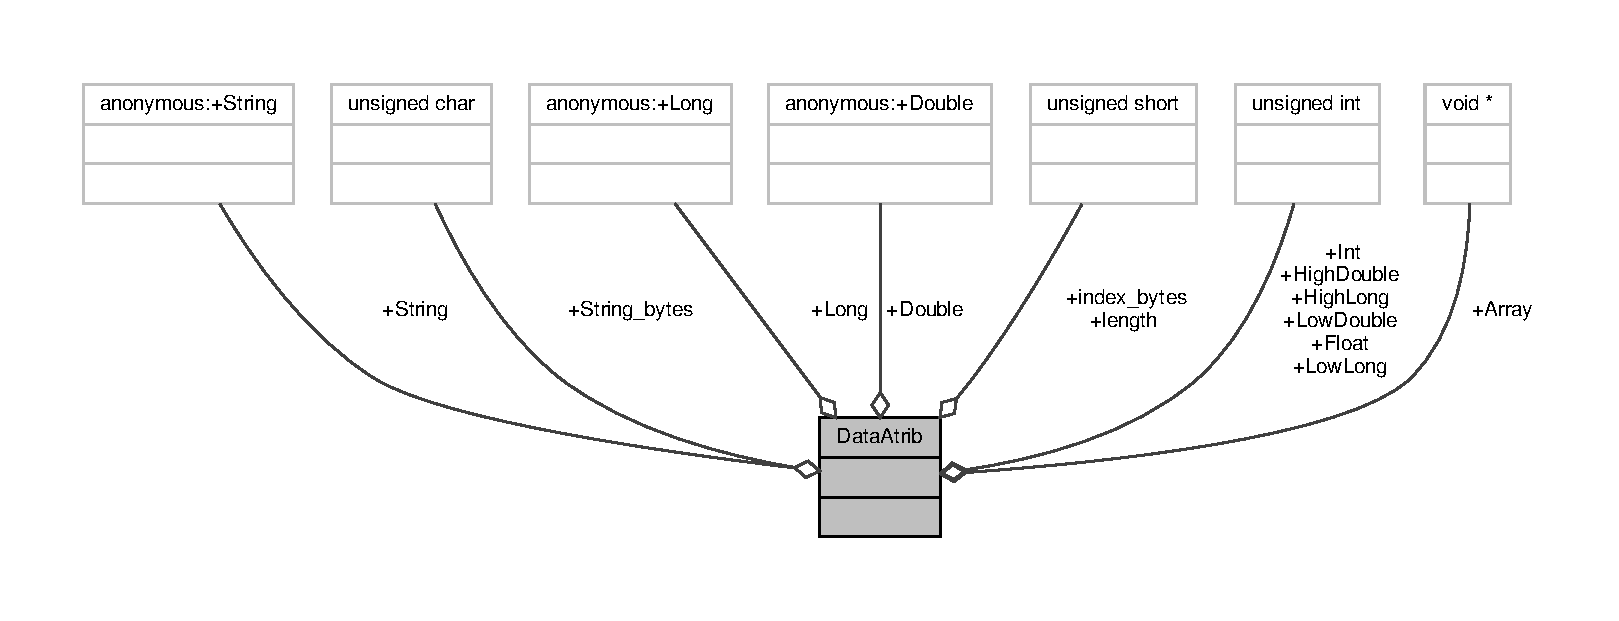
\includegraphics[width=350pt]{unionDataAtrib__coll__graph}
\end{center}
\end{figure}
\subsection*{Atributos Públicos}
\begin{DoxyCompactItemize}
\item 
\begin{tabbing}
xx\=xx\=xx\=xx\=xx\=xx\=xx\=xx\=xx\=\kill
struct \{\\
\>\hyperlink{ClassLoader_8h_a5f223212eef04d10a4550ded680cb1cf}{u2} \hyperlink{unionDataAtrib_afca160cb9b44b9af18bd6b84156cabbe}{length}\\
\>\hyperlink{ClassLoader_8h_a216a9f8b04b4f0af84a4ca9d1d85a6ca}{u1} $\ast$ \hyperlink{unionDataAtrib_a6ed5174c66346d1713654b70b363eef7}{String\_bytes}\\
\>\hyperlink{ClassLoader_8h_a5f223212eef04d10a4550ded680cb1cf}{u2} \hyperlink{unionDataAtrib_a534a316e72c85094ad85664a845eae7f}{index\_bytes}\\
\} \hyperlink{unionDataAtrib_a2d7e4f85a56b23c89a93ca99c6dcefaf}{String}\\

\end{tabbing}\item 
\hyperlink{ClassLoader_8h_aedf6ddc03df8caaaccbb4c60b9a9b850}{u4} \hyperlink{unionDataAtrib_a0ceb91dbaf5366fb7b7aeb8bd940d0ce}{Int}
\item 
void $\ast$ \hyperlink{unionDataAtrib_a1cd92c3acf2b8cbe2889f0b766661f1d}{Array}
\item 
\begin{tabbing}
xx\=xx\=xx\=xx\=xx\=xx\=xx\=xx\=xx\=\kill
struct \{\\
\>\hyperlink{ClassLoader_8h_aedf6ddc03df8caaaccbb4c60b9a9b850}{u4} \hyperlink{unionDataAtrib_abb7703b7239c1c10a4f0dd2564af85cf}{LowLong}\\
\>\hyperlink{ClassLoader_8h_aedf6ddc03df8caaaccbb4c60b9a9b850}{u4} \hyperlink{unionDataAtrib_a517700e20f5cbaeeb1c6ba0003ee4c12}{HighLong}\\
\} \hyperlink{unionDataAtrib_af58e31949f8075f641fc9dd016fc187e}{Long}\\

\end{tabbing}\item 
\hyperlink{ClassLoader_8h_aedf6ddc03df8caaaccbb4c60b9a9b850}{u4} \hyperlink{unionDataAtrib_abf1cacd5fc8d6219aa5bea2dc474f89a}{Float}
\item 
\begin{tabbing}
xx\=xx\=xx\=xx\=xx\=xx\=xx\=xx\=xx\=\kill
struct \{\\
\>\hyperlink{ClassLoader_8h_aedf6ddc03df8caaaccbb4c60b9a9b850}{u4} \hyperlink{unionDataAtrib_a1f6e08d1c97fee36f6b0f92d7b985933}{LowDouble}\\
\>\hyperlink{ClassLoader_8h_aedf6ddc03df8caaaccbb4c60b9a9b850}{u4} \hyperlink{unionDataAtrib_ae701e4461c45e996636b301026eec3e1}{HighDouble}\\
\} \hyperlink{unionDataAtrib_ab9a5f070a06a259aad6e82f068fc305f}{Double}\\

\end{tabbing}\end{DoxyCompactItemize}


\subsection{Descrição Detalhada}
Estrutura que gerencia os atributos dinâmicos para cada tipo. 

\subsection{Atributos}
\mbox{\Hypertarget{unionDataAtrib_a1cd92c3acf2b8cbe2889f0b766661f1d}\label{unionDataAtrib_a1cd92c3acf2b8cbe2889f0b766661f1d}} 
\index{Data\+Atrib@{Data\+Atrib}!Array@{Array}}
\index{Array@{Array}!Data\+Atrib@{Data\+Atrib}}
\subsubsection{\texorpdfstring{Array}{Array}}
{\footnotesize\ttfamily void$\ast$ Data\+Atrib\+::\+Array}

\mbox{\Hypertarget{unionDataAtrib_ab9a5f070a06a259aad6e82f068fc305f}\label{unionDataAtrib_ab9a5f070a06a259aad6e82f068fc305f}} 
\index{Data\+Atrib@{Data\+Atrib}!Double@{Double}}
\index{Double@{Double}!Data\+Atrib@{Data\+Atrib}}
\subsubsection{\texorpdfstring{Double}{Double}}
{\footnotesize\ttfamily struct \{ ... \}  Data\+Atrib\+::\+Double}

\mbox{\Hypertarget{unionDataAtrib_abf1cacd5fc8d6219aa5bea2dc474f89a}\label{unionDataAtrib_abf1cacd5fc8d6219aa5bea2dc474f89a}} 
\index{Data\+Atrib@{Data\+Atrib}!Float@{Float}}
\index{Float@{Float}!Data\+Atrib@{Data\+Atrib}}
\subsubsection{\texorpdfstring{Float}{Float}}
{\footnotesize\ttfamily \hyperlink{ClassLoader_8h_aedf6ddc03df8caaaccbb4c60b9a9b850}{u4} Data\+Atrib\+::\+Float}

\mbox{\Hypertarget{unionDataAtrib_ae701e4461c45e996636b301026eec3e1}\label{unionDataAtrib_ae701e4461c45e996636b301026eec3e1}} 
\index{Data\+Atrib@{Data\+Atrib}!High\+Double@{High\+Double}}
\index{High\+Double@{High\+Double}!Data\+Atrib@{Data\+Atrib}}
\subsubsection{\texorpdfstring{High\+Double}{HighDouble}}
{\footnotesize\ttfamily \hyperlink{ClassLoader_8h_aedf6ddc03df8caaaccbb4c60b9a9b850}{u4} Data\+Atrib\+::\+High\+Double}

\mbox{\Hypertarget{unionDataAtrib_a517700e20f5cbaeeb1c6ba0003ee4c12}\label{unionDataAtrib_a517700e20f5cbaeeb1c6ba0003ee4c12}} 
\index{Data\+Atrib@{Data\+Atrib}!High\+Long@{High\+Long}}
\index{High\+Long@{High\+Long}!Data\+Atrib@{Data\+Atrib}}
\subsubsection{\texorpdfstring{High\+Long}{HighLong}}
{\footnotesize\ttfamily \hyperlink{ClassLoader_8h_aedf6ddc03df8caaaccbb4c60b9a9b850}{u4} Data\+Atrib\+::\+High\+Long}

\mbox{\Hypertarget{unionDataAtrib_a534a316e72c85094ad85664a845eae7f}\label{unionDataAtrib_a534a316e72c85094ad85664a845eae7f}} 
\index{Data\+Atrib@{Data\+Atrib}!index\+\_\+bytes@{index\+\_\+bytes}}
\index{index\+\_\+bytes@{index\+\_\+bytes}!Data\+Atrib@{Data\+Atrib}}
\subsubsection{\texorpdfstring{index\+\_\+bytes}{index\_bytes}}
{\footnotesize\ttfamily \hyperlink{ClassLoader_8h_a5f223212eef04d10a4550ded680cb1cf}{u2} Data\+Atrib\+::index\+\_\+bytes}

\mbox{\Hypertarget{unionDataAtrib_a0ceb91dbaf5366fb7b7aeb8bd940d0ce}\label{unionDataAtrib_a0ceb91dbaf5366fb7b7aeb8bd940d0ce}} 
\index{Data\+Atrib@{Data\+Atrib}!Int@{Int}}
\index{Int@{Int}!Data\+Atrib@{Data\+Atrib}}
\subsubsection{\texorpdfstring{Int}{Int}}
{\footnotesize\ttfamily \hyperlink{ClassLoader_8h_aedf6ddc03df8caaaccbb4c60b9a9b850}{u4} Data\+Atrib\+::\+Int}

\mbox{\Hypertarget{unionDataAtrib_afca160cb9b44b9af18bd6b84156cabbe}\label{unionDataAtrib_afca160cb9b44b9af18bd6b84156cabbe}} 
\index{Data\+Atrib@{Data\+Atrib}!length@{length}}
\index{length@{length}!Data\+Atrib@{Data\+Atrib}}
\subsubsection{\texorpdfstring{length}{length}}
{\footnotesize\ttfamily \hyperlink{ClassLoader_8h_a5f223212eef04d10a4550ded680cb1cf}{u2} Data\+Atrib\+::length}

\mbox{\Hypertarget{unionDataAtrib_af58e31949f8075f641fc9dd016fc187e}\label{unionDataAtrib_af58e31949f8075f641fc9dd016fc187e}} 
\index{Data\+Atrib@{Data\+Atrib}!Long@{Long}}
\index{Long@{Long}!Data\+Atrib@{Data\+Atrib}}
\subsubsection{\texorpdfstring{Long}{Long}}
{\footnotesize\ttfamily struct \{ ... \}  Data\+Atrib\+::\+Long}

\mbox{\Hypertarget{unionDataAtrib_a1f6e08d1c97fee36f6b0f92d7b985933}\label{unionDataAtrib_a1f6e08d1c97fee36f6b0f92d7b985933}} 
\index{Data\+Atrib@{Data\+Atrib}!Low\+Double@{Low\+Double}}
\index{Low\+Double@{Low\+Double}!Data\+Atrib@{Data\+Atrib}}
\subsubsection{\texorpdfstring{Low\+Double}{LowDouble}}
{\footnotesize\ttfamily \hyperlink{ClassLoader_8h_aedf6ddc03df8caaaccbb4c60b9a9b850}{u4} Data\+Atrib\+::\+Low\+Double}

\mbox{\Hypertarget{unionDataAtrib_abb7703b7239c1c10a4f0dd2564af85cf}\label{unionDataAtrib_abb7703b7239c1c10a4f0dd2564af85cf}} 
\index{Data\+Atrib@{Data\+Atrib}!Low\+Long@{Low\+Long}}
\index{Low\+Long@{Low\+Long}!Data\+Atrib@{Data\+Atrib}}
\subsubsection{\texorpdfstring{Low\+Long}{LowLong}}
{\footnotesize\ttfamily \hyperlink{ClassLoader_8h_aedf6ddc03df8caaaccbb4c60b9a9b850}{u4} Data\+Atrib\+::\+Low\+Long}

\mbox{\Hypertarget{unionDataAtrib_a2d7e4f85a56b23c89a93ca99c6dcefaf}\label{unionDataAtrib_a2d7e4f85a56b23c89a93ca99c6dcefaf}} 
\index{Data\+Atrib@{Data\+Atrib}!String@{String}}
\index{String@{String}!Data\+Atrib@{Data\+Atrib}}
\subsubsection{\texorpdfstring{String}{String}}
{\footnotesize\ttfamily struct \{ ... \}  Data\+Atrib\+::\+String}

\mbox{\Hypertarget{unionDataAtrib_a6ed5174c66346d1713654b70b363eef7}\label{unionDataAtrib_a6ed5174c66346d1713654b70b363eef7}} 
\index{Data\+Atrib@{Data\+Atrib}!String\+\_\+bytes@{String\+\_\+bytes}}
\index{String\+\_\+bytes@{String\+\_\+bytes}!Data\+Atrib@{Data\+Atrib}}
\subsubsection{\texorpdfstring{String\+\_\+bytes}{String\_bytes}}
{\footnotesize\ttfamily \hyperlink{ClassLoader_8h_a216a9f8b04b4f0af84a4ca9d1d85a6ca}{u1}$\ast$ Data\+Atrib\+::\+String\+\_\+bytes}



A documentação para esta união foi gerada a partir do seguinte arquivo\+:\begin{DoxyCompactItemize}
\item 
\hyperlink{MethodArea_8h}{Method\+Area.\+h}\end{DoxyCompactItemize}

\hypertarget{unionattribute__info_1_1dataatt}{}\section{Referência da União attribute\+\_\+info\+:\+:dataatt}
\label{unionattribute__info_1_1dataatt}\index{attribute\+\_\+info\+::dataatt@{attribute\+\_\+info\+::dataatt}}


{\ttfamily \#include $<$Class\+Loader.\+h$>$}



Diagrama de colaboração para attribute\+\_\+info\+:\+:dataatt\+:\nopagebreak
\begin{figure}[H]
\begin{center}
\leavevmode
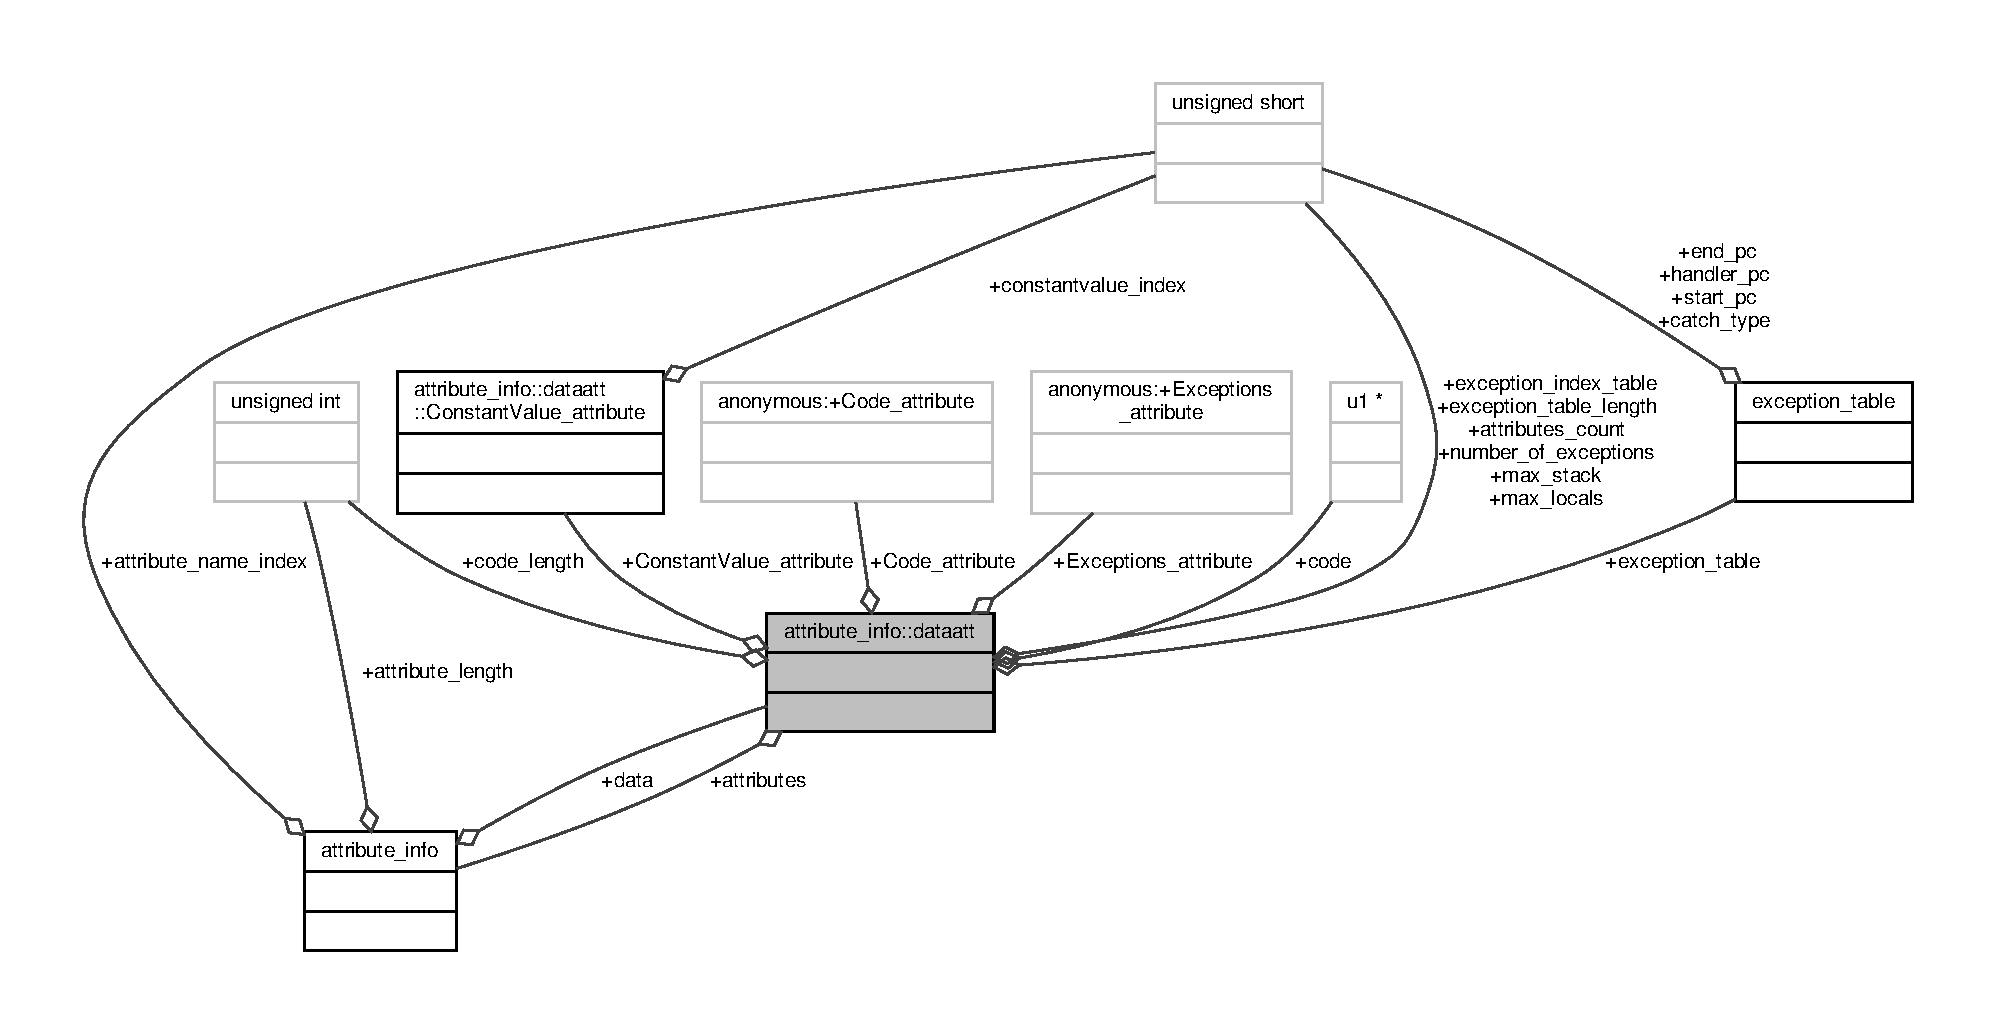
\includegraphics[width=350pt]{unionattribute__info_1_1dataatt__coll__graph}
\end{center}
\end{figure}
\subsection*{Componentes}
\begin{DoxyCompactItemize}
\item 
struct \hyperlink{structattribute__info_1_1dataatt_1_1ConstantValue__attribute}{Constant\+Value\+\_\+attribute}
\end{DoxyCompactItemize}
\subsection*{Atributos Públicos}
\begin{DoxyCompactItemize}
\item 
struct \hyperlink{structattribute__info_1_1dataatt_1_1ConstantValue__attribute}{attribute\+\_\+info\+::dataatt\+::\+Constant\+Value\+\_\+attribute} \hyperlink{unionattribute__info_1_1dataatt_a7528732c04d522ee66b03ac3ee68a328}{Constant\+Value\+\_\+attribute}
\item 
\begin{tabbing}
xx\=xx\=xx\=xx\=xx\=xx\=xx\=xx\=xx\=\kill
struct \{\\
\>\hyperlink{ClassLoader_8h_a5f223212eef04d10a4550ded680cb1cf}{u2} \hyperlink{unionattribute__info_1_1dataatt_a5324cb4f9387dd83fbf918a214e9ecf5}{max\_stack}\\
\>\hyperlink{ClassLoader_8h_a5f223212eef04d10a4550ded680cb1cf}{u2} \hyperlink{unionattribute__info_1_1dataatt_a50f68cdf74cc0a4ae6cfdff4f9deff56}{max\_locals}\\
\>\hyperlink{ClassLoader_8h_aedf6ddc03df8caaaccbb4c60b9a9b850}{u4} \hyperlink{unionattribute__info_1_1dataatt_a632ec76b539aef919ad1b53bc06ae202}{code\_length}\\
\>\hyperlink{ClassLoader_8h_a216a9f8b04b4f0af84a4ca9d1d85a6ca}{u1} $\ast$ \hyperlink{unionattribute__info_1_1dataatt_ae358021d0aeaf42c2946d7ca9bde4561}{code}\\
\>\hyperlink{ClassLoader_8h_a5f223212eef04d10a4550ded680cb1cf}{u2} \hyperlink{unionattribute__info_1_1dataatt_aab4fba017aae830c5d0ee6e5498c4e0a}{exception\_table\_length}\\
\>struct \hyperlink{structexception__table}{exception\_table} $\ast$ \hyperlink{unionattribute__info_1_1dataatt_ad8651df15e6a1ce7795fb5bbfc036497}{exception\_table}\\
\>\hyperlink{ClassLoader_8h_a5f223212eef04d10a4550ded680cb1cf}{u2} \hyperlink{unionattribute__info_1_1dataatt_a2684a4c2f7e2e9bf618563c5aa3f0bad}{attributes\_count}\\
\>struct \hyperlink{structattribute__info}{attribute\_info} $\ast$ \hyperlink{unionattribute__info_1_1dataatt_a3e6b34fe04111fe1a6b2d386d7c7e4f3}{attributes}\\
\} \hyperlink{unionattribute__info_1_1dataatt_ab0774fa2b3c172330d4428a0be7c9819}{Code\_attribute}\\

\end{tabbing}\item 
\begin{tabbing}
xx\=xx\=xx\=xx\=xx\=xx\=xx\=xx\=xx\=\kill
struct \{\\
\>\hyperlink{ClassLoader_8h_a5f223212eef04d10a4550ded680cb1cf}{u2} \hyperlink{unionattribute__info_1_1dataatt_a6c0783aaa8139388956c2d325ea0e904}{number\_of\_exceptions}\\
\>\hyperlink{ClassLoader_8h_a5f223212eef04d10a4550ded680cb1cf}{u2} $\ast$ \hyperlink{unionattribute__info_1_1dataatt_ac88c57d4da20ece664c3c9afda924cdc}{exception\_index\_table}\\
\} \hyperlink{unionattribute__info_1_1dataatt_ad7f5003a6c7d5c548721a8a85be1b640}{Exceptions\_attribute}\\

\end{tabbing}\item 
\begin{tabbing}
xx\=xx\=xx\=xx\=xx\=xx\=xx\=xx\=xx\=\kill
struct \{\\
\>\hyperlink{ClassLoader_8h_a5f223212eef04d10a4550ded680cb1cf}{u2} \hyperlink{unionattribute__info_1_1dataatt_ae0da9bc25d733475ae813bc0e68eafdd}{number\_of\_classes}\\
\>\hyperlink{structclasstype__info}{classtype\_info} $\ast$ \hyperlink{unionattribute__info_1_1dataatt_a6ee27f7185933597c714148102b5b753}{classes}\\
\} \hyperlink{unionattribute__info_1_1dataatt_a4e2aef7107d3492718555c31ed9dd090}{InnerClasses}\\

\end{tabbing}\item 
\begin{tabbing}
xx\=xx\=xx\=xx\=xx\=xx\=xx\=xx\=xx\=\kill
struct \{\\
\>\hyperlink{ClassLoader_8h_a216a9f8b04b4f0af84a4ca9d1d85a6ca}{u1} $\ast$ \hyperlink{unionattribute__info_1_1dataatt_ae8d3932b5cb732fecb7f21c6d629b97d}{bytes}\\
\} \hyperlink{unionattribute__info_1_1dataatt_af88f44781ffe638c91492186db4c77b6}{Other}\\

\end{tabbing}\end{DoxyCompactItemize}


\subsection{Atributos}
\mbox{\Hypertarget{unionattribute__info_1_1dataatt_a3e6b34fe04111fe1a6b2d386d7c7e4f3}\label{unionattribute__info_1_1dataatt_a3e6b34fe04111fe1a6b2d386d7c7e4f3}} 
\index{attribute\+\_\+info\+::dataatt@{attribute\+\_\+info\+::dataatt}!attributes@{attributes}}
\index{attributes@{attributes}!attribute\+\_\+info\+::dataatt@{attribute\+\_\+info\+::dataatt}}
\subsubsection{\texorpdfstring{attributes}{attributes}}
{\footnotesize\ttfamily struct \hyperlink{structattribute__info}{attribute\+\_\+info}$\ast$ attribute\+\_\+info\+::dataatt\+::attributes}

\mbox{\Hypertarget{unionattribute__info_1_1dataatt_a2684a4c2f7e2e9bf618563c5aa3f0bad}\label{unionattribute__info_1_1dataatt_a2684a4c2f7e2e9bf618563c5aa3f0bad}} 
\index{attribute\+\_\+info\+::dataatt@{attribute\+\_\+info\+::dataatt}!attributes\+\_\+count@{attributes\+\_\+count}}
\index{attributes\+\_\+count@{attributes\+\_\+count}!attribute\+\_\+info\+::dataatt@{attribute\+\_\+info\+::dataatt}}
\subsubsection{\texorpdfstring{attributes\+\_\+count}{attributes\_count}}
{\footnotesize\ttfamily \hyperlink{ClassLoader_8h_a5f223212eef04d10a4550ded680cb1cf}{u2} attribute\+\_\+info\+::dataatt\+::attributes\+\_\+count}

\mbox{\Hypertarget{unionattribute__info_1_1dataatt_ae8d3932b5cb732fecb7f21c6d629b97d}\label{unionattribute__info_1_1dataatt_ae8d3932b5cb732fecb7f21c6d629b97d}} 
\index{attribute\+\_\+info\+::dataatt@{attribute\+\_\+info\+::dataatt}!bytes@{bytes}}
\index{bytes@{bytes}!attribute\+\_\+info\+::dataatt@{attribute\+\_\+info\+::dataatt}}
\subsubsection{\texorpdfstring{bytes}{bytes}}
{\footnotesize\ttfamily \hyperlink{ClassLoader_8h_a216a9f8b04b4f0af84a4ca9d1d85a6ca}{u1}$\ast$ attribute\+\_\+info\+::dataatt\+::bytes}

\mbox{\Hypertarget{unionattribute__info_1_1dataatt_a6ee27f7185933597c714148102b5b753}\label{unionattribute__info_1_1dataatt_a6ee27f7185933597c714148102b5b753}} 
\index{attribute\+\_\+info\+::dataatt@{attribute\+\_\+info\+::dataatt}!classes@{classes}}
\index{classes@{classes}!attribute\+\_\+info\+::dataatt@{attribute\+\_\+info\+::dataatt}}
\subsubsection{\texorpdfstring{classes}{classes}}
{\footnotesize\ttfamily \hyperlink{structclasstype__info}{classtype\+\_\+info}$\ast$ attribute\+\_\+info\+::dataatt\+::classes}

\mbox{\Hypertarget{unionattribute__info_1_1dataatt_ae358021d0aeaf42c2946d7ca9bde4561}\label{unionattribute__info_1_1dataatt_ae358021d0aeaf42c2946d7ca9bde4561}} 
\index{attribute\+\_\+info\+::dataatt@{attribute\+\_\+info\+::dataatt}!code@{code}}
\index{code@{code}!attribute\+\_\+info\+::dataatt@{attribute\+\_\+info\+::dataatt}}
\subsubsection{\texorpdfstring{code}{code}}
{\footnotesize\ttfamily \hyperlink{ClassLoader_8h_a216a9f8b04b4f0af84a4ca9d1d85a6ca}{u1}$\ast$ attribute\+\_\+info\+::dataatt\+::code}

\mbox{\Hypertarget{unionattribute__info_1_1dataatt_ab0774fa2b3c172330d4428a0be7c9819}\label{unionattribute__info_1_1dataatt_ab0774fa2b3c172330d4428a0be7c9819}} 
\index{attribute\+\_\+info\+::dataatt@{attribute\+\_\+info\+::dataatt}!Code\+\_\+attribute@{Code\+\_\+attribute}}
\index{Code\+\_\+attribute@{Code\+\_\+attribute}!attribute\+\_\+info\+::dataatt@{attribute\+\_\+info\+::dataatt}}
\subsubsection{\texorpdfstring{Code\+\_\+attribute}{Code\_attribute}}
{\footnotesize\ttfamily struct \{ ... \}  attribute\+\_\+info\+::dataatt\+::\+Code\+\_\+attribute}

\mbox{\Hypertarget{unionattribute__info_1_1dataatt_a632ec76b539aef919ad1b53bc06ae202}\label{unionattribute__info_1_1dataatt_a632ec76b539aef919ad1b53bc06ae202}} 
\index{attribute\+\_\+info\+::dataatt@{attribute\+\_\+info\+::dataatt}!code\+\_\+length@{code\+\_\+length}}
\index{code\+\_\+length@{code\+\_\+length}!attribute\+\_\+info\+::dataatt@{attribute\+\_\+info\+::dataatt}}
\subsubsection{\texorpdfstring{code\+\_\+length}{code\_length}}
{\footnotesize\ttfamily \hyperlink{ClassLoader_8h_aedf6ddc03df8caaaccbb4c60b9a9b850}{u4} attribute\+\_\+info\+::dataatt\+::code\+\_\+length}

\mbox{\Hypertarget{unionattribute__info_1_1dataatt_a7528732c04d522ee66b03ac3ee68a328}\label{unionattribute__info_1_1dataatt_a7528732c04d522ee66b03ac3ee68a328}} 
\index{attribute\+\_\+info\+::dataatt@{attribute\+\_\+info\+::dataatt}!Constant\+Value\+\_\+attribute@{Constant\+Value\+\_\+attribute}}
\index{Constant\+Value\+\_\+attribute@{Constant\+Value\+\_\+attribute}!attribute\+\_\+info\+::dataatt@{attribute\+\_\+info\+::dataatt}}
\subsubsection{\texorpdfstring{Constant\+Value\+\_\+attribute}{ConstantValue\_attribute}}
{\footnotesize\ttfamily struct \hyperlink{structattribute__info_1_1dataatt_1_1ConstantValue__attribute}{attribute\+\_\+info\+::dataatt\+::\+Constant\+Value\+\_\+attribute} \hyperlink{structattribute__info_1_1dataatt_1_1ConstantValue__attribute}{attribute\+\_\+info\+::dataatt\+::\+Constant\+Value\+\_\+attribute}}

\mbox{\Hypertarget{unionattribute__info_1_1dataatt_ac88c57d4da20ece664c3c9afda924cdc}\label{unionattribute__info_1_1dataatt_ac88c57d4da20ece664c3c9afda924cdc}} 
\index{attribute\+\_\+info\+::dataatt@{attribute\+\_\+info\+::dataatt}!exception\+\_\+index\+\_\+table@{exception\+\_\+index\+\_\+table}}
\index{exception\+\_\+index\+\_\+table@{exception\+\_\+index\+\_\+table}!attribute\+\_\+info\+::dataatt@{attribute\+\_\+info\+::dataatt}}
\subsubsection{\texorpdfstring{exception\+\_\+index\+\_\+table}{exception\_index\_table}}
{\footnotesize\ttfamily \hyperlink{ClassLoader_8h_a5f223212eef04d10a4550ded680cb1cf}{u2}$\ast$ attribute\+\_\+info\+::dataatt\+::exception\+\_\+index\+\_\+table}

\mbox{\Hypertarget{unionattribute__info_1_1dataatt_ad8651df15e6a1ce7795fb5bbfc036497}\label{unionattribute__info_1_1dataatt_ad8651df15e6a1ce7795fb5bbfc036497}} 
\index{attribute\+\_\+info\+::dataatt@{attribute\+\_\+info\+::dataatt}!exception\+\_\+table@{exception\+\_\+table}}
\index{exception\+\_\+table@{exception\+\_\+table}!attribute\+\_\+info\+::dataatt@{attribute\+\_\+info\+::dataatt}}
\subsubsection{\texorpdfstring{exception\+\_\+table}{exception\_table}}
{\footnotesize\ttfamily struct \hyperlink{structexception__table}{exception\+\_\+table}$\ast$ attribute\+\_\+info\+::dataatt\+::exception\+\_\+table}

\mbox{\Hypertarget{unionattribute__info_1_1dataatt_aab4fba017aae830c5d0ee6e5498c4e0a}\label{unionattribute__info_1_1dataatt_aab4fba017aae830c5d0ee6e5498c4e0a}} 
\index{attribute\+\_\+info\+::dataatt@{attribute\+\_\+info\+::dataatt}!exception\+\_\+table\+\_\+length@{exception\+\_\+table\+\_\+length}}
\index{exception\+\_\+table\+\_\+length@{exception\+\_\+table\+\_\+length}!attribute\+\_\+info\+::dataatt@{attribute\+\_\+info\+::dataatt}}
\subsubsection{\texorpdfstring{exception\+\_\+table\+\_\+length}{exception\_table\_length}}
{\footnotesize\ttfamily \hyperlink{ClassLoader_8h_a5f223212eef04d10a4550ded680cb1cf}{u2} attribute\+\_\+info\+::dataatt\+::exception\+\_\+table\+\_\+length}

\mbox{\Hypertarget{unionattribute__info_1_1dataatt_ad7f5003a6c7d5c548721a8a85be1b640}\label{unionattribute__info_1_1dataatt_ad7f5003a6c7d5c548721a8a85be1b640}} 
\index{attribute\+\_\+info\+::dataatt@{attribute\+\_\+info\+::dataatt}!Exceptions\+\_\+attribute@{Exceptions\+\_\+attribute}}
\index{Exceptions\+\_\+attribute@{Exceptions\+\_\+attribute}!attribute\+\_\+info\+::dataatt@{attribute\+\_\+info\+::dataatt}}
\subsubsection{\texorpdfstring{Exceptions\+\_\+attribute}{Exceptions\_attribute}}
{\footnotesize\ttfamily struct \{ ... \}  attribute\+\_\+info\+::dataatt\+::\+Exceptions\+\_\+attribute}

\mbox{\Hypertarget{unionattribute__info_1_1dataatt_a4e2aef7107d3492718555c31ed9dd090}\label{unionattribute__info_1_1dataatt_a4e2aef7107d3492718555c31ed9dd090}} 
\index{attribute\+\_\+info\+::dataatt@{attribute\+\_\+info\+::dataatt}!Inner\+Classes@{Inner\+Classes}}
\index{Inner\+Classes@{Inner\+Classes}!attribute\+\_\+info\+::dataatt@{attribute\+\_\+info\+::dataatt}}
\subsubsection{\texorpdfstring{Inner\+Classes}{InnerClasses}}
{\footnotesize\ttfamily struct \{ ... \}     attribute\+\_\+info\+::dataatt\+::\+Inner\+Classes}

\mbox{\Hypertarget{unionattribute__info_1_1dataatt_a50f68cdf74cc0a4ae6cfdff4f9deff56}\label{unionattribute__info_1_1dataatt_a50f68cdf74cc0a4ae6cfdff4f9deff56}} 
\index{attribute\+\_\+info\+::dataatt@{attribute\+\_\+info\+::dataatt}!max\+\_\+locals@{max\+\_\+locals}}
\index{max\+\_\+locals@{max\+\_\+locals}!attribute\+\_\+info\+::dataatt@{attribute\+\_\+info\+::dataatt}}
\subsubsection{\texorpdfstring{max\+\_\+locals}{max\_locals}}
{\footnotesize\ttfamily \hyperlink{ClassLoader_8h_a5f223212eef04d10a4550ded680cb1cf}{u2} attribute\+\_\+info\+::dataatt\+::max\+\_\+locals}

\mbox{\Hypertarget{unionattribute__info_1_1dataatt_a5324cb4f9387dd83fbf918a214e9ecf5}\label{unionattribute__info_1_1dataatt_a5324cb4f9387dd83fbf918a214e9ecf5}} 
\index{attribute\+\_\+info\+::dataatt@{attribute\+\_\+info\+::dataatt}!max\+\_\+stack@{max\+\_\+stack}}
\index{max\+\_\+stack@{max\+\_\+stack}!attribute\+\_\+info\+::dataatt@{attribute\+\_\+info\+::dataatt}}
\subsubsection{\texorpdfstring{max\+\_\+stack}{max\_stack}}
{\footnotesize\ttfamily \hyperlink{ClassLoader_8h_a5f223212eef04d10a4550ded680cb1cf}{u2} attribute\+\_\+info\+::dataatt\+::max\+\_\+stack}

\mbox{\Hypertarget{unionattribute__info_1_1dataatt_ae0da9bc25d733475ae813bc0e68eafdd}\label{unionattribute__info_1_1dataatt_ae0da9bc25d733475ae813bc0e68eafdd}} 
\index{attribute\+\_\+info\+::dataatt@{attribute\+\_\+info\+::dataatt}!number\+\_\+of\+\_\+classes@{number\+\_\+of\+\_\+classes}}
\index{number\+\_\+of\+\_\+classes@{number\+\_\+of\+\_\+classes}!attribute\+\_\+info\+::dataatt@{attribute\+\_\+info\+::dataatt}}
\subsubsection{\texorpdfstring{number\+\_\+of\+\_\+classes}{number\_of\_classes}}
{\footnotesize\ttfamily \hyperlink{ClassLoader_8h_a5f223212eef04d10a4550ded680cb1cf}{u2} attribute\+\_\+info\+::dataatt\+::number\+\_\+of\+\_\+classes}

\mbox{\Hypertarget{unionattribute__info_1_1dataatt_a6c0783aaa8139388956c2d325ea0e904}\label{unionattribute__info_1_1dataatt_a6c0783aaa8139388956c2d325ea0e904}} 
\index{attribute\+\_\+info\+::dataatt@{attribute\+\_\+info\+::dataatt}!number\+\_\+of\+\_\+exceptions@{number\+\_\+of\+\_\+exceptions}}
\index{number\+\_\+of\+\_\+exceptions@{number\+\_\+of\+\_\+exceptions}!attribute\+\_\+info\+::dataatt@{attribute\+\_\+info\+::dataatt}}
\subsubsection{\texorpdfstring{number\+\_\+of\+\_\+exceptions}{number\_of\_exceptions}}
{\footnotesize\ttfamily \hyperlink{ClassLoader_8h_a5f223212eef04d10a4550ded680cb1cf}{u2} attribute\+\_\+info\+::dataatt\+::number\+\_\+of\+\_\+exceptions}

\mbox{\Hypertarget{unionattribute__info_1_1dataatt_af88f44781ffe638c91492186db4c77b6}\label{unionattribute__info_1_1dataatt_af88f44781ffe638c91492186db4c77b6}} 
\index{attribute\+\_\+info\+::dataatt@{attribute\+\_\+info\+::dataatt}!Other@{Other}}
\index{Other@{Other}!attribute\+\_\+info\+::dataatt@{attribute\+\_\+info\+::dataatt}}
\subsubsection{\texorpdfstring{Other}{Other}}
{\footnotesize\ttfamily struct \{ ... \}   attribute\+\_\+info\+::dataatt\+::\+Other}



A documentação para esta união foi gerada a partir do seguinte arquivo\+:\begin{DoxyCompactItemize}
\item 
\hyperlink{ClassLoader_8h}{Class\+Loader.\+h}\end{DoxyCompactItemize}

\hypertarget{unioncp__info_1_1datacp}{}\section{Referência da União cp\+\_\+info\+:\+:datacp}
\label{unioncp__info_1_1datacp}\index{cp\+\_\+info\+::datacp@{cp\+\_\+info\+::datacp}}


{\ttfamily \#include $<$Class\+Loader.\+h$>$}



Diagrama de colaboração para cp\+\_\+info\+:\+:datacp\+:
\nopagebreak
\begin{figure}[H]
\begin{center}
\leavevmode
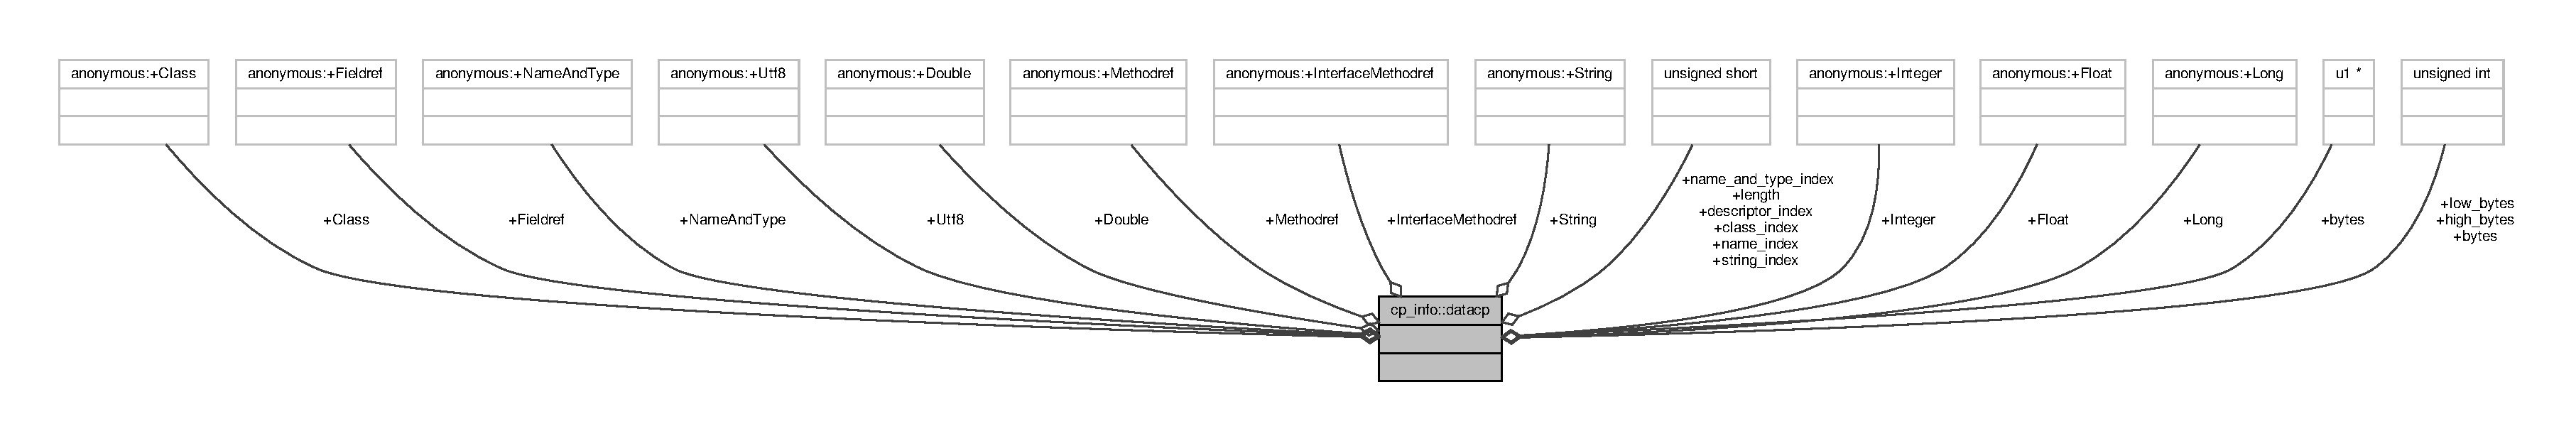
\includegraphics[width=350pt]{unioncp__info_1_1datacp__coll__graph}
\end{center}
\end{figure}
\subsection*{Atributos Públicos}
\begin{DoxyCompactItemize}
\item 
\begin{tabbing}
xx\=xx\=xx\=xx\=xx\=xx\=xx\=xx\=xx\=\kill
struct \{\\
\>\hyperlink{ClassLoader_8h_a5f223212eef04d10a4550ded680cb1cf}{u2} \hyperlink{unioncp__info_1_1datacp_a4540b43d9ad83000fc7febdba3cfef4a}{name\_index}\\
\} \hyperlink{unioncp__info_1_1datacp_ae475c9d491733ff6d6d87965005cb376}{Class}\\

\end{tabbing}\item 
\begin{tabbing}
xx\=xx\=xx\=xx\=xx\=xx\=xx\=xx\=xx\=\kill
struct \{\\
\>\hyperlink{ClassLoader_8h_a5f223212eef04d10a4550ded680cb1cf}{u2} \hyperlink{unioncp__info_1_1datacp_afe58e71caa77c751cd4149cba08365c9}{class\_index}\\
\>\hyperlink{ClassLoader_8h_a5f223212eef04d10a4550ded680cb1cf}{u2} \hyperlink{unioncp__info_1_1datacp_a10e647455d27f6b08b65df60301401d9}{name\_and\_type\_index}\\
\} \hyperlink{unioncp__info_1_1datacp_ad3c92f312ae43399774a3833cf0c1fb0}{Fieldref}\\

\end{tabbing}\item 
\begin{tabbing}
xx\=xx\=xx\=xx\=xx\=xx\=xx\=xx\=xx\=\kill
struct \{\\
\>\hyperlink{ClassLoader_8h_a5f223212eef04d10a4550ded680cb1cf}{u2} \hyperlink{unioncp__info_1_1datacp_a4540b43d9ad83000fc7febdba3cfef4a}{name\_index}\\
\>\hyperlink{ClassLoader_8h_a5f223212eef04d10a4550ded680cb1cf}{u2} \hyperlink{unioncp__info_1_1datacp_a9dd2cf98a0eacfc287bf71858e5ca7fb}{descriptor\_index}\\
\} \hyperlink{unioncp__info_1_1datacp_ad886d3026fc0887dbc19058dd29ad2de}{NameAndType}\\

\end{tabbing}\item 
\begin{tabbing}
xx\=xx\=xx\=xx\=xx\=xx\=xx\=xx\=xx\=\kill
struct \{\\
\>\hyperlink{ClassLoader_8h_a5f223212eef04d10a4550ded680cb1cf}{u2} \hyperlink{unioncp__info_1_1datacp_a38d5e0a1710a66be36faaa9ca4c0beb7}{length}\\
\>\hyperlink{ClassLoader_8h_a216a9f8b04b4f0af84a4ca9d1d85a6ca}{u1} $\ast$ \hyperlink{unioncp__info_1_1datacp_a40e488bf00f85faac8a0fb14fabea614}{bytes}\\
\} \hyperlink{unioncp__info_1_1datacp_ad1597573ef20c04564d00878897378be}{Utf8}\\

\end{tabbing}\item 
\begin{tabbing}
xx\=xx\=xx\=xx\=xx\=xx\=xx\=xx\=xx\=\kill
struct \{\\
\>\hyperlink{ClassLoader_8h_a5f223212eef04d10a4550ded680cb1cf}{u2} \hyperlink{unioncp__info_1_1datacp_afe58e71caa77c751cd4149cba08365c9}{class\_index}\\
\>\hyperlink{ClassLoader_8h_a5f223212eef04d10a4550ded680cb1cf}{u2} \hyperlink{unioncp__info_1_1datacp_a10e647455d27f6b08b65df60301401d9}{name\_and\_type\_index}\\
\} \hyperlink{unioncp__info_1_1datacp_a67ad4ffccbde7fe06759c612ad3c8ffd}{Methodref}\\

\end{tabbing}\item 
\begin{tabbing}
xx\=xx\=xx\=xx\=xx\=xx\=xx\=xx\=xx\=\kill
struct \{\\
\>\hyperlink{ClassLoader_8h_a5f223212eef04d10a4550ded680cb1cf}{u2} \hyperlink{unioncp__info_1_1datacp_afe58e71caa77c751cd4149cba08365c9}{class\_index}\\
\>\hyperlink{ClassLoader_8h_a5f223212eef04d10a4550ded680cb1cf}{u2} \hyperlink{unioncp__info_1_1datacp_a10e647455d27f6b08b65df60301401d9}{name\_and\_type\_index}\\
\} \hyperlink{unioncp__info_1_1datacp_a74c3eb4bdff29dc50efbafc145e6c3a8}{InterfaceMethodref}\\

\end{tabbing}\item 
\begin{tabbing}
xx\=xx\=xx\=xx\=xx\=xx\=xx\=xx\=xx\=\kill
struct \{\\
\>\hyperlink{ClassLoader_8h_a5f223212eef04d10a4550ded680cb1cf}{u2} \hyperlink{unioncp__info_1_1datacp_af0c3e4590189a854d4c52d70464571cf}{string\_index}\\
\} \hyperlink{unioncp__info_1_1datacp_adbed25f7609825c7bfb2d5e5df502498}{String}\\

\end{tabbing}\item 
\begin{tabbing}
xx\=xx\=xx\=xx\=xx\=xx\=xx\=xx\=xx\=\kill
struct \{\\
\>\hyperlink{ClassLoader_8h_aedf6ddc03df8caaaccbb4c60b9a9b850}{u4} \hyperlink{unioncp__info_1_1datacp_ac52b232a2050869b907c4f779040ae55}{bytes}\\
\} \hyperlink{unioncp__info_1_1datacp_a7aec2d971b32d3928dc02a07caf7277f}{Integer}\\

\end{tabbing}\item 
\begin{tabbing}
xx\=xx\=xx\=xx\=xx\=xx\=xx\=xx\=xx\=\kill
struct \{\\
\>\hyperlink{ClassLoader_8h_aedf6ddc03df8caaaccbb4c60b9a9b850}{u4} \hyperlink{unioncp__info_1_1datacp_ac52b232a2050869b907c4f779040ae55}{bytes}\\
\} \hyperlink{unioncp__info_1_1datacp_a8337d31eeb14be90eea1b63fcb89203f}{Float}\\

\end{tabbing}\item 
\begin{tabbing}
xx\=xx\=xx\=xx\=xx\=xx\=xx\=xx\=xx\=\kill
struct \{\\
\>\hyperlink{ClassLoader_8h_aedf6ddc03df8caaaccbb4c60b9a9b850}{u4} \hyperlink{unioncp__info_1_1datacp_a31f14c5e0d6b0cd8886188564f5544ca}{high\_bytes}\\
\>\hyperlink{ClassLoader_8h_aedf6ddc03df8caaaccbb4c60b9a9b850}{u4} \hyperlink{unioncp__info_1_1datacp_a4851a5181dd7496139fa419eb5351d49}{low\_bytes}\\
\} \hyperlink{unioncp__info_1_1datacp_ac234c2addabca2e1c120faf4557de4dc}{Long}\\

\end{tabbing}\item 
\begin{tabbing}
xx\=xx\=xx\=xx\=xx\=xx\=xx\=xx\=xx\=\kill
struct \{\\
\>\hyperlink{ClassLoader_8h_aedf6ddc03df8caaaccbb4c60b9a9b850}{u4} \hyperlink{unioncp__info_1_1datacp_a31f14c5e0d6b0cd8886188564f5544ca}{high\_bytes}\\
\>\hyperlink{ClassLoader_8h_aedf6ddc03df8caaaccbb4c60b9a9b850}{u4} \hyperlink{unioncp__info_1_1datacp_a4851a5181dd7496139fa419eb5351d49}{low\_bytes}\\
\} \hyperlink{unioncp__info_1_1datacp_a3be6ec0a488ed9cce7fe4ae1fe68b95c}{Double}\\

\end{tabbing}\end{DoxyCompactItemize}


\subsection{Atributos}
\mbox{\Hypertarget{unioncp__info_1_1datacp_a40e488bf00f85faac8a0fb14fabea614}\label{unioncp__info_1_1datacp_a40e488bf00f85faac8a0fb14fabea614}} 
\index{cp\+\_\+info\+::datacp@{cp\+\_\+info\+::datacp}!bytes@{bytes}}
\index{bytes@{bytes}!cp\+\_\+info\+::datacp@{cp\+\_\+info\+::datacp}}
\subsubsection{\texorpdfstring{bytes}{bytes}\hspace{0.1cm}{\footnotesize\ttfamily [1/2]}}
{\footnotesize\ttfamily \hyperlink{ClassLoader_8h_a216a9f8b04b4f0af84a4ca9d1d85a6ca}{u1}$\ast$ cp\+\_\+info\+::datacp\+::bytes}

\mbox{\Hypertarget{unioncp__info_1_1datacp_ac52b232a2050869b907c4f779040ae55}\label{unioncp__info_1_1datacp_ac52b232a2050869b907c4f779040ae55}} 
\index{cp\+\_\+info\+::datacp@{cp\+\_\+info\+::datacp}!bytes@{bytes}}
\index{bytes@{bytes}!cp\+\_\+info\+::datacp@{cp\+\_\+info\+::datacp}}
\subsubsection{\texorpdfstring{bytes}{bytes}\hspace{0.1cm}{\footnotesize\ttfamily [2/2]}}
{\footnotesize\ttfamily \hyperlink{ClassLoader_8h_aedf6ddc03df8caaaccbb4c60b9a9b850}{u4} cp\+\_\+info\+::datacp\+::bytes}

\mbox{\Hypertarget{unioncp__info_1_1datacp_ae475c9d491733ff6d6d87965005cb376}\label{unioncp__info_1_1datacp_ae475c9d491733ff6d6d87965005cb376}} 
\index{cp\+\_\+info\+::datacp@{cp\+\_\+info\+::datacp}!Class@{Class}}
\index{Class@{Class}!cp\+\_\+info\+::datacp@{cp\+\_\+info\+::datacp}}
\subsubsection{\texorpdfstring{Class}{Class}}
{\footnotesize\ttfamily struct \{ ... \}  cp\+\_\+info\+::datacp\+::\+Class}

\mbox{\Hypertarget{unioncp__info_1_1datacp_afe58e71caa77c751cd4149cba08365c9}\label{unioncp__info_1_1datacp_afe58e71caa77c751cd4149cba08365c9}} 
\index{cp\+\_\+info\+::datacp@{cp\+\_\+info\+::datacp}!class\+\_\+index@{class\+\_\+index}}
\index{class\+\_\+index@{class\+\_\+index}!cp\+\_\+info\+::datacp@{cp\+\_\+info\+::datacp}}
\subsubsection{\texorpdfstring{class\+\_\+index}{class\_index}}
{\footnotesize\ttfamily \hyperlink{ClassLoader_8h_a5f223212eef04d10a4550ded680cb1cf}{u2} cp\+\_\+info\+::datacp\+::class\+\_\+index}

\mbox{\Hypertarget{unioncp__info_1_1datacp_a9dd2cf98a0eacfc287bf71858e5ca7fb}\label{unioncp__info_1_1datacp_a9dd2cf98a0eacfc287bf71858e5ca7fb}} 
\index{cp\+\_\+info\+::datacp@{cp\+\_\+info\+::datacp}!descriptor\+\_\+index@{descriptor\+\_\+index}}
\index{descriptor\+\_\+index@{descriptor\+\_\+index}!cp\+\_\+info\+::datacp@{cp\+\_\+info\+::datacp}}
\subsubsection{\texorpdfstring{descriptor\+\_\+index}{descriptor\_index}}
{\footnotesize\ttfamily \hyperlink{ClassLoader_8h_a5f223212eef04d10a4550ded680cb1cf}{u2} cp\+\_\+info\+::datacp\+::descriptor\+\_\+index}

\mbox{\Hypertarget{unioncp__info_1_1datacp_a3be6ec0a488ed9cce7fe4ae1fe68b95c}\label{unioncp__info_1_1datacp_a3be6ec0a488ed9cce7fe4ae1fe68b95c}} 
\index{cp\+\_\+info\+::datacp@{cp\+\_\+info\+::datacp}!Double@{Double}}
\index{Double@{Double}!cp\+\_\+info\+::datacp@{cp\+\_\+info\+::datacp}}
\subsubsection{\texorpdfstring{Double}{Double}}
{\footnotesize\ttfamily struct \{ ... \}  cp\+\_\+info\+::datacp\+::\+Double}

\mbox{\Hypertarget{unioncp__info_1_1datacp_ad3c92f312ae43399774a3833cf0c1fb0}\label{unioncp__info_1_1datacp_ad3c92f312ae43399774a3833cf0c1fb0}} 
\index{cp\+\_\+info\+::datacp@{cp\+\_\+info\+::datacp}!Fieldref@{Fieldref}}
\index{Fieldref@{Fieldref}!cp\+\_\+info\+::datacp@{cp\+\_\+info\+::datacp}}
\subsubsection{\texorpdfstring{Fieldref}{Fieldref}}
{\footnotesize\ttfamily struct \{ ... \}  cp\+\_\+info\+::datacp\+::\+Fieldref}

\mbox{\Hypertarget{unioncp__info_1_1datacp_a8337d31eeb14be90eea1b63fcb89203f}\label{unioncp__info_1_1datacp_a8337d31eeb14be90eea1b63fcb89203f}} 
\index{cp\+\_\+info\+::datacp@{cp\+\_\+info\+::datacp}!Float@{Float}}
\index{Float@{Float}!cp\+\_\+info\+::datacp@{cp\+\_\+info\+::datacp}}
\subsubsection{\texorpdfstring{Float}{Float}}
{\footnotesize\ttfamily struct \{ ... \}  cp\+\_\+info\+::datacp\+::\+Float}

\mbox{\Hypertarget{unioncp__info_1_1datacp_a31f14c5e0d6b0cd8886188564f5544ca}\label{unioncp__info_1_1datacp_a31f14c5e0d6b0cd8886188564f5544ca}} 
\index{cp\+\_\+info\+::datacp@{cp\+\_\+info\+::datacp}!high\+\_\+bytes@{high\+\_\+bytes}}
\index{high\+\_\+bytes@{high\+\_\+bytes}!cp\+\_\+info\+::datacp@{cp\+\_\+info\+::datacp}}
\subsubsection{\texorpdfstring{high\+\_\+bytes}{high\_bytes}}
{\footnotesize\ttfamily \hyperlink{ClassLoader_8h_aedf6ddc03df8caaaccbb4c60b9a9b850}{u4} cp\+\_\+info\+::datacp\+::high\+\_\+bytes}

\mbox{\Hypertarget{unioncp__info_1_1datacp_a7aec2d971b32d3928dc02a07caf7277f}\label{unioncp__info_1_1datacp_a7aec2d971b32d3928dc02a07caf7277f}} 
\index{cp\+\_\+info\+::datacp@{cp\+\_\+info\+::datacp}!Integer@{Integer}}
\index{Integer@{Integer}!cp\+\_\+info\+::datacp@{cp\+\_\+info\+::datacp}}
\subsubsection{\texorpdfstring{Integer}{Integer}}
{\footnotesize\ttfamily struct \{ ... \}  cp\+\_\+info\+::datacp\+::\+Integer}

\mbox{\Hypertarget{unioncp__info_1_1datacp_a74c3eb4bdff29dc50efbafc145e6c3a8}\label{unioncp__info_1_1datacp_a74c3eb4bdff29dc50efbafc145e6c3a8}} 
\index{cp\+\_\+info\+::datacp@{cp\+\_\+info\+::datacp}!Interface\+Methodref@{Interface\+Methodref}}
\index{Interface\+Methodref@{Interface\+Methodref}!cp\+\_\+info\+::datacp@{cp\+\_\+info\+::datacp}}
\subsubsection{\texorpdfstring{Interface\+Methodref}{InterfaceMethodref}}
{\footnotesize\ttfamily struct \{ ... \}  cp\+\_\+info\+::datacp\+::\+Interface\+Methodref}

\mbox{\Hypertarget{unioncp__info_1_1datacp_a38d5e0a1710a66be36faaa9ca4c0beb7}\label{unioncp__info_1_1datacp_a38d5e0a1710a66be36faaa9ca4c0beb7}} 
\index{cp\+\_\+info\+::datacp@{cp\+\_\+info\+::datacp}!length@{length}}
\index{length@{length}!cp\+\_\+info\+::datacp@{cp\+\_\+info\+::datacp}}
\subsubsection{\texorpdfstring{length}{length}}
{\footnotesize\ttfamily \hyperlink{ClassLoader_8h_a5f223212eef04d10a4550ded680cb1cf}{u2} cp\+\_\+info\+::datacp\+::length}

\mbox{\Hypertarget{unioncp__info_1_1datacp_ac234c2addabca2e1c120faf4557de4dc}\label{unioncp__info_1_1datacp_ac234c2addabca2e1c120faf4557de4dc}} 
\index{cp\+\_\+info\+::datacp@{cp\+\_\+info\+::datacp}!Long@{Long}}
\index{Long@{Long}!cp\+\_\+info\+::datacp@{cp\+\_\+info\+::datacp}}
\subsubsection{\texorpdfstring{Long}{Long}}
{\footnotesize\ttfamily struct \{ ... \}  cp\+\_\+info\+::datacp\+::\+Long}

\mbox{\Hypertarget{unioncp__info_1_1datacp_a4851a5181dd7496139fa419eb5351d49}\label{unioncp__info_1_1datacp_a4851a5181dd7496139fa419eb5351d49}} 
\index{cp\+\_\+info\+::datacp@{cp\+\_\+info\+::datacp}!low\+\_\+bytes@{low\+\_\+bytes}}
\index{low\+\_\+bytes@{low\+\_\+bytes}!cp\+\_\+info\+::datacp@{cp\+\_\+info\+::datacp}}
\subsubsection{\texorpdfstring{low\+\_\+bytes}{low\_bytes}}
{\footnotesize\ttfamily \hyperlink{ClassLoader_8h_aedf6ddc03df8caaaccbb4c60b9a9b850}{u4} cp\+\_\+info\+::datacp\+::low\+\_\+bytes}

\mbox{\Hypertarget{unioncp__info_1_1datacp_a67ad4ffccbde7fe06759c612ad3c8ffd}\label{unioncp__info_1_1datacp_a67ad4ffccbde7fe06759c612ad3c8ffd}} 
\index{cp\+\_\+info\+::datacp@{cp\+\_\+info\+::datacp}!Methodref@{Methodref}}
\index{Methodref@{Methodref}!cp\+\_\+info\+::datacp@{cp\+\_\+info\+::datacp}}
\subsubsection{\texorpdfstring{Methodref}{Methodref}}
{\footnotesize\ttfamily struct \{ ... \}  cp\+\_\+info\+::datacp\+::\+Methodref}

\mbox{\Hypertarget{unioncp__info_1_1datacp_a10e647455d27f6b08b65df60301401d9}\label{unioncp__info_1_1datacp_a10e647455d27f6b08b65df60301401d9}} 
\index{cp\+\_\+info\+::datacp@{cp\+\_\+info\+::datacp}!name\+\_\+and\+\_\+type\+\_\+index@{name\+\_\+and\+\_\+type\+\_\+index}}
\index{name\+\_\+and\+\_\+type\+\_\+index@{name\+\_\+and\+\_\+type\+\_\+index}!cp\+\_\+info\+::datacp@{cp\+\_\+info\+::datacp}}
\subsubsection{\texorpdfstring{name\+\_\+and\+\_\+type\+\_\+index}{name\_and\_type\_index}}
{\footnotesize\ttfamily \hyperlink{ClassLoader_8h_a5f223212eef04d10a4550ded680cb1cf}{u2} cp\+\_\+info\+::datacp\+::name\+\_\+and\+\_\+type\+\_\+index}

\mbox{\Hypertarget{unioncp__info_1_1datacp_a4540b43d9ad83000fc7febdba3cfef4a}\label{unioncp__info_1_1datacp_a4540b43d9ad83000fc7febdba3cfef4a}} 
\index{cp\+\_\+info\+::datacp@{cp\+\_\+info\+::datacp}!name\+\_\+index@{name\+\_\+index}}
\index{name\+\_\+index@{name\+\_\+index}!cp\+\_\+info\+::datacp@{cp\+\_\+info\+::datacp}}
\subsubsection{\texorpdfstring{name\+\_\+index}{name\_index}}
{\footnotesize\ttfamily \hyperlink{ClassLoader_8h_a5f223212eef04d10a4550ded680cb1cf}{u2} cp\+\_\+info\+::datacp\+::name\+\_\+index}

\mbox{\Hypertarget{unioncp__info_1_1datacp_ad886d3026fc0887dbc19058dd29ad2de}\label{unioncp__info_1_1datacp_ad886d3026fc0887dbc19058dd29ad2de}} 
\index{cp\+\_\+info\+::datacp@{cp\+\_\+info\+::datacp}!Name\+And\+Type@{Name\+And\+Type}}
\index{Name\+And\+Type@{Name\+And\+Type}!cp\+\_\+info\+::datacp@{cp\+\_\+info\+::datacp}}
\subsubsection{\texorpdfstring{Name\+And\+Type}{NameAndType}}
{\footnotesize\ttfamily struct \{ ... \}  cp\+\_\+info\+::datacp\+::\+Name\+And\+Type}

\mbox{\Hypertarget{unioncp__info_1_1datacp_adbed25f7609825c7bfb2d5e5df502498}\label{unioncp__info_1_1datacp_adbed25f7609825c7bfb2d5e5df502498}} 
\index{cp\+\_\+info\+::datacp@{cp\+\_\+info\+::datacp}!String@{String}}
\index{String@{String}!cp\+\_\+info\+::datacp@{cp\+\_\+info\+::datacp}}
\subsubsection{\texorpdfstring{String}{String}}
{\footnotesize\ttfamily struct \{ ... \}  cp\+\_\+info\+::datacp\+::\+String}

\mbox{\Hypertarget{unioncp__info_1_1datacp_af0c3e4590189a854d4c52d70464571cf}\label{unioncp__info_1_1datacp_af0c3e4590189a854d4c52d70464571cf}} 
\index{cp\+\_\+info\+::datacp@{cp\+\_\+info\+::datacp}!string\+\_\+index@{string\+\_\+index}}
\index{string\+\_\+index@{string\+\_\+index}!cp\+\_\+info\+::datacp@{cp\+\_\+info\+::datacp}}
\subsubsection{\texorpdfstring{string\+\_\+index}{string\_index}}
{\footnotesize\ttfamily \hyperlink{ClassLoader_8h_a5f223212eef04d10a4550ded680cb1cf}{u2} cp\+\_\+info\+::datacp\+::string\+\_\+index}

\mbox{\Hypertarget{unioncp__info_1_1datacp_ad1597573ef20c04564d00878897378be}\label{unioncp__info_1_1datacp_ad1597573ef20c04564d00878897378be}} 
\index{cp\+\_\+info\+::datacp@{cp\+\_\+info\+::datacp}!Utf8@{Utf8}}
\index{Utf8@{Utf8}!cp\+\_\+info\+::datacp@{cp\+\_\+info\+::datacp}}
\subsubsection{\texorpdfstring{Utf8}{Utf8}}
{\footnotesize\ttfamily struct \{ ... \}  cp\+\_\+info\+::datacp\+::\+Utf8}



A documentação para esta união foi gerada a partir do seguinte arquivo\+:\begin{DoxyCompactItemize}
\item 
\hyperlink{ClassLoader_8h}{Class\+Loader.\+h}\end{DoxyCompactItemize}

\hypertarget{unionDataStaticAtrib}{}\section{Referência da União Data\+Static\+Atrib}
\label{unionDataStaticAtrib}\index{Data\+Static\+Atrib@{Data\+Static\+Atrib}}


Estrutura que gerencia os atributos estáticos para cada tipo.  




{\ttfamily \#include $<$Method\+Area.\+h$>$}



Diagrama de colaboração para Data\+Static\+Atrib\+:
\nopagebreak
\begin{figure}[H]
\begin{center}
\leavevmode
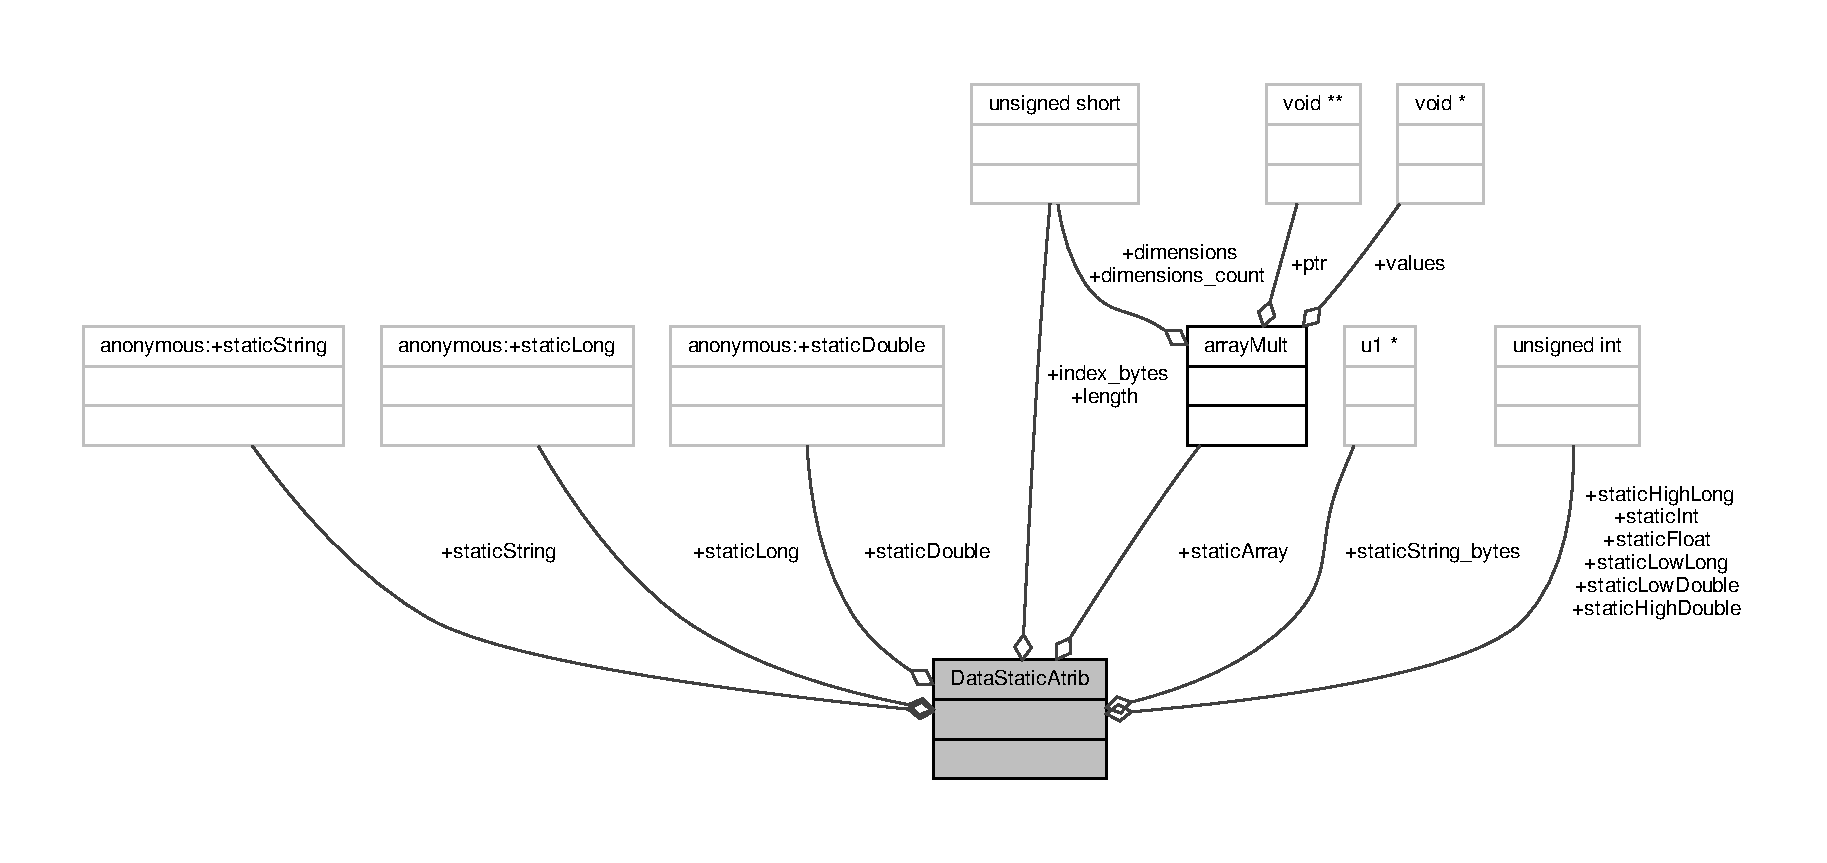
\includegraphics[width=350pt]{unionDataStaticAtrib__coll__graph}
\end{center}
\end{figure}
\subsection*{Atributos Públicos}
\begin{DoxyCompactItemize}
\item 
\begin{tabbing}
xx\=xx\=xx\=xx\=xx\=xx\=xx\=xx\=xx\=\kill
struct \{\\
\>\hyperlink{ClassLoader_8h_a5f223212eef04d10a4550ded680cb1cf}{u2} \hyperlink{unionDataStaticAtrib_a30e703ce693927359d7f287e11b379e8}{length}\\
\>\hyperlink{ClassLoader_8h_a216a9f8b04b4f0af84a4ca9d1d85a6ca}{u1} $\ast$ \hyperlink{unionDataStaticAtrib_ab578dc394ef2a6b255e56724317bfb0a}{staticString\_bytes}\\
\>\hyperlink{ClassLoader_8h_a5f223212eef04d10a4550ded680cb1cf}{u2} \hyperlink{unionDataStaticAtrib_ada02ebc6846de921edad741e3052b40e}{index\_bytes}\\
\} \hyperlink{unionDataStaticAtrib_a74a2c8f98d0cc1708e4a97050c73ed3f}{staticString}\\

\end{tabbing}\item 
\hyperlink{ClassLoader_8h_aedf6ddc03df8caaaccbb4c60b9a9b850}{u4} \hyperlink{unionDataStaticAtrib_ae7a8bb0c0d974245fa446f5a81a73708}{static\+Int}
\item 
\hyperlink{structarrayMult}{array\+Mult} $\ast$ \hyperlink{unionDataStaticAtrib_a418b97f9c6821b2a14419daec27dd8f8}{static\+Array}
\item 
\begin{tabbing}
xx\=xx\=xx\=xx\=xx\=xx\=xx\=xx\=xx\=\kill
struct \{\\
\>\hyperlink{ClassLoader_8h_aedf6ddc03df8caaaccbb4c60b9a9b850}{u4} \hyperlink{unionDataStaticAtrib_aa04959b5aa4875d47c56624692ce0bb3}{staticLowLong}\\
\>\hyperlink{ClassLoader_8h_aedf6ddc03df8caaaccbb4c60b9a9b850}{u4} \hyperlink{unionDataStaticAtrib_a4ba29f20a7aed050ec0ac87f157659ed}{staticHighLong}\\
\} \hyperlink{unionDataStaticAtrib_a4b7ba61e5437a798e69114d4ecbf813d}{staticLong}\\

\end{tabbing}\item 
\hyperlink{ClassLoader_8h_aedf6ddc03df8caaaccbb4c60b9a9b850}{u4} \hyperlink{unionDataStaticAtrib_a9ad6975d8a8bbc1b4587aad4077fc6c8}{static\+Float}
\item 
\begin{tabbing}
xx\=xx\=xx\=xx\=xx\=xx\=xx\=xx\=xx\=\kill
struct \{\\
\>\hyperlink{ClassLoader_8h_aedf6ddc03df8caaaccbb4c60b9a9b850}{u4} \hyperlink{unionDataStaticAtrib_a8ee07b1e266aef56917b0d24be2766e4}{staticLowDouble}\\
\>\hyperlink{ClassLoader_8h_aedf6ddc03df8caaaccbb4c60b9a9b850}{u4} \hyperlink{unionDataStaticAtrib_a64fbbc4728f4f98aa2fb483f5ab3110b}{staticHighDouble}\\
\} \hyperlink{unionDataStaticAtrib_a0c72eaebd5ce5602a9181140c217dcee}{staticDouble}\\

\end{tabbing}\end{DoxyCompactItemize}


\subsection{Descrição Detalhada}
Estrutura que gerencia os atributos estáticos para cada tipo. 

\subsection{Atributos}
\mbox{\Hypertarget{unionDataStaticAtrib_ada02ebc6846de921edad741e3052b40e}\label{unionDataStaticAtrib_ada02ebc6846de921edad741e3052b40e}} 
\index{Data\+Static\+Atrib@{Data\+Static\+Atrib}!index\+\_\+bytes@{index\+\_\+bytes}}
\index{index\+\_\+bytes@{index\+\_\+bytes}!Data\+Static\+Atrib@{Data\+Static\+Atrib}}
\subsubsection{\texorpdfstring{index\+\_\+bytes}{index\_bytes}}
{\footnotesize\ttfamily \hyperlink{ClassLoader_8h_a5f223212eef04d10a4550ded680cb1cf}{u2} Data\+Static\+Atrib\+::index\+\_\+bytes}

\mbox{\Hypertarget{unionDataStaticAtrib_a30e703ce693927359d7f287e11b379e8}\label{unionDataStaticAtrib_a30e703ce693927359d7f287e11b379e8}} 
\index{Data\+Static\+Atrib@{Data\+Static\+Atrib}!length@{length}}
\index{length@{length}!Data\+Static\+Atrib@{Data\+Static\+Atrib}}
\subsubsection{\texorpdfstring{length}{length}}
{\footnotesize\ttfamily \hyperlink{ClassLoader_8h_a5f223212eef04d10a4550ded680cb1cf}{u2} Data\+Static\+Atrib\+::length}

\mbox{\Hypertarget{unionDataStaticAtrib_a418b97f9c6821b2a14419daec27dd8f8}\label{unionDataStaticAtrib_a418b97f9c6821b2a14419daec27dd8f8}} 
\index{Data\+Static\+Atrib@{Data\+Static\+Atrib}!static\+Array@{static\+Array}}
\index{static\+Array@{static\+Array}!Data\+Static\+Atrib@{Data\+Static\+Atrib}}
\subsubsection{\texorpdfstring{static\+Array}{staticArray}}
{\footnotesize\ttfamily \hyperlink{structarrayMult}{array\+Mult}$\ast$ Data\+Static\+Atrib\+::static\+Array}

\mbox{\Hypertarget{unionDataStaticAtrib_a0c72eaebd5ce5602a9181140c217dcee}\label{unionDataStaticAtrib_a0c72eaebd5ce5602a9181140c217dcee}} 
\index{Data\+Static\+Atrib@{Data\+Static\+Atrib}!static\+Double@{static\+Double}}
\index{static\+Double@{static\+Double}!Data\+Static\+Atrib@{Data\+Static\+Atrib}}
\subsubsection{\texorpdfstring{static\+Double}{staticDouble}}
{\footnotesize\ttfamily struct \{ ... \}  Data\+Static\+Atrib\+::static\+Double}

\mbox{\Hypertarget{unionDataStaticAtrib_a9ad6975d8a8bbc1b4587aad4077fc6c8}\label{unionDataStaticAtrib_a9ad6975d8a8bbc1b4587aad4077fc6c8}} 
\index{Data\+Static\+Atrib@{Data\+Static\+Atrib}!static\+Float@{static\+Float}}
\index{static\+Float@{static\+Float}!Data\+Static\+Atrib@{Data\+Static\+Atrib}}
\subsubsection{\texorpdfstring{static\+Float}{staticFloat}}
{\footnotesize\ttfamily \hyperlink{ClassLoader_8h_aedf6ddc03df8caaaccbb4c60b9a9b850}{u4} Data\+Static\+Atrib\+::static\+Float}

\mbox{\Hypertarget{unionDataStaticAtrib_a64fbbc4728f4f98aa2fb483f5ab3110b}\label{unionDataStaticAtrib_a64fbbc4728f4f98aa2fb483f5ab3110b}} 
\index{Data\+Static\+Atrib@{Data\+Static\+Atrib}!static\+High\+Double@{static\+High\+Double}}
\index{static\+High\+Double@{static\+High\+Double}!Data\+Static\+Atrib@{Data\+Static\+Atrib}}
\subsubsection{\texorpdfstring{static\+High\+Double}{staticHighDouble}}
{\footnotesize\ttfamily \hyperlink{ClassLoader_8h_aedf6ddc03df8caaaccbb4c60b9a9b850}{u4} Data\+Static\+Atrib\+::static\+High\+Double}

\mbox{\Hypertarget{unionDataStaticAtrib_a4ba29f20a7aed050ec0ac87f157659ed}\label{unionDataStaticAtrib_a4ba29f20a7aed050ec0ac87f157659ed}} 
\index{Data\+Static\+Atrib@{Data\+Static\+Atrib}!static\+High\+Long@{static\+High\+Long}}
\index{static\+High\+Long@{static\+High\+Long}!Data\+Static\+Atrib@{Data\+Static\+Atrib}}
\subsubsection{\texorpdfstring{static\+High\+Long}{staticHighLong}}
{\footnotesize\ttfamily \hyperlink{ClassLoader_8h_aedf6ddc03df8caaaccbb4c60b9a9b850}{u4} Data\+Static\+Atrib\+::static\+High\+Long}

\mbox{\Hypertarget{unionDataStaticAtrib_ae7a8bb0c0d974245fa446f5a81a73708}\label{unionDataStaticAtrib_ae7a8bb0c0d974245fa446f5a81a73708}} 
\index{Data\+Static\+Atrib@{Data\+Static\+Atrib}!static\+Int@{static\+Int}}
\index{static\+Int@{static\+Int}!Data\+Static\+Atrib@{Data\+Static\+Atrib}}
\subsubsection{\texorpdfstring{static\+Int}{staticInt}}
{\footnotesize\ttfamily \hyperlink{ClassLoader_8h_aedf6ddc03df8caaaccbb4c60b9a9b850}{u4} Data\+Static\+Atrib\+::static\+Int}

\mbox{\Hypertarget{unionDataStaticAtrib_a4b7ba61e5437a798e69114d4ecbf813d}\label{unionDataStaticAtrib_a4b7ba61e5437a798e69114d4ecbf813d}} 
\index{Data\+Static\+Atrib@{Data\+Static\+Atrib}!static\+Long@{static\+Long}}
\index{static\+Long@{static\+Long}!Data\+Static\+Atrib@{Data\+Static\+Atrib}}
\subsubsection{\texorpdfstring{static\+Long}{staticLong}}
{\footnotesize\ttfamily struct \{ ... \}  Data\+Static\+Atrib\+::static\+Long}

\mbox{\Hypertarget{unionDataStaticAtrib_a8ee07b1e266aef56917b0d24be2766e4}\label{unionDataStaticAtrib_a8ee07b1e266aef56917b0d24be2766e4}} 
\index{Data\+Static\+Atrib@{Data\+Static\+Atrib}!static\+Low\+Double@{static\+Low\+Double}}
\index{static\+Low\+Double@{static\+Low\+Double}!Data\+Static\+Atrib@{Data\+Static\+Atrib}}
\subsubsection{\texorpdfstring{static\+Low\+Double}{staticLowDouble}}
{\footnotesize\ttfamily \hyperlink{ClassLoader_8h_aedf6ddc03df8caaaccbb4c60b9a9b850}{u4} Data\+Static\+Atrib\+::static\+Low\+Double}

\mbox{\Hypertarget{unionDataStaticAtrib_aa04959b5aa4875d47c56624692ce0bb3}\label{unionDataStaticAtrib_aa04959b5aa4875d47c56624692ce0bb3}} 
\index{Data\+Static\+Atrib@{Data\+Static\+Atrib}!static\+Low\+Long@{static\+Low\+Long}}
\index{static\+Low\+Long@{static\+Low\+Long}!Data\+Static\+Atrib@{Data\+Static\+Atrib}}
\subsubsection{\texorpdfstring{static\+Low\+Long}{staticLowLong}}
{\footnotesize\ttfamily \hyperlink{ClassLoader_8h_aedf6ddc03df8caaaccbb4c60b9a9b850}{u4} Data\+Static\+Atrib\+::static\+Low\+Long}

\mbox{\Hypertarget{unionDataStaticAtrib_a74a2c8f98d0cc1708e4a97050c73ed3f}\label{unionDataStaticAtrib_a74a2c8f98d0cc1708e4a97050c73ed3f}} 
\index{Data\+Static\+Atrib@{Data\+Static\+Atrib}!static\+String@{static\+String}}
\index{static\+String@{static\+String}!Data\+Static\+Atrib@{Data\+Static\+Atrib}}
\subsubsection{\texorpdfstring{static\+String}{staticString}}
{\footnotesize\ttfamily struct \{ ... \}  Data\+Static\+Atrib\+::static\+String}

\mbox{\Hypertarget{unionDataStaticAtrib_ab578dc394ef2a6b255e56724317bfb0a}\label{unionDataStaticAtrib_ab578dc394ef2a6b255e56724317bfb0a}} 
\index{Data\+Static\+Atrib@{Data\+Static\+Atrib}!static\+String\+\_\+bytes@{static\+String\+\_\+bytes}}
\index{static\+String\+\_\+bytes@{static\+String\+\_\+bytes}!Data\+Static\+Atrib@{Data\+Static\+Atrib}}
\subsubsection{\texorpdfstring{static\+String\+\_\+bytes}{staticString\_bytes}}
{\footnotesize\ttfamily \hyperlink{ClassLoader_8h_a216a9f8b04b4f0af84a4ca9d1d85a6ca}{u1}$\ast$ Data\+Static\+Atrib\+::static\+String\+\_\+bytes}



A documentação para esta união foi gerada a partir do seguinte arquivo\+:\begin{DoxyCompactItemize}
\item 
\hyperlink{MethodArea_8h}{Method\+Area.\+h}\end{DoxyCompactItemize}

\hypertarget{structexception__table}{}\section{Referência da Estrutura exception\+\_\+table}
\label{structexception__table}\index{exception\+\_\+table@{exception\+\_\+table}}


Tabela de excesões.  




{\ttfamily \#include $<$Class\+Loader.\+h$>$}



Diagrama de colaboração para exception\+\_\+table\+:\nopagebreak
\begin{figure}[H]
\begin{center}
\leavevmode
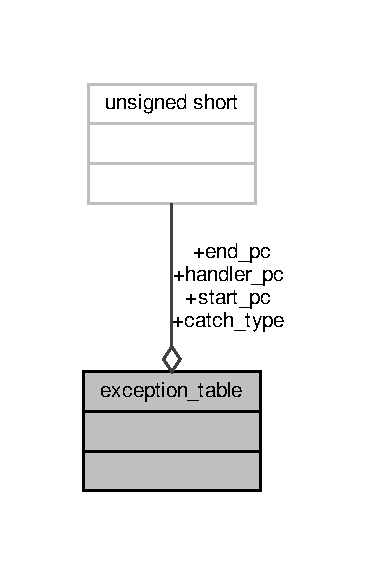
\includegraphics[width=178pt]{structexception__table__coll__graph}
\end{center}
\end{figure}
\subsection*{Atributos Públicos}
\begin{DoxyCompactItemize}
\item 
\hyperlink{ClassLoader_8h_a5f223212eef04d10a4550ded680cb1cf}{u2} \hyperlink{structexception__table_a63da93a2b0f5dc61b3a158a0c7384602}{start\+\_\+pc}
\item 
\hyperlink{ClassLoader_8h_a5f223212eef04d10a4550ded680cb1cf}{u2} \hyperlink{structexception__table_aeb4c86c92f02d6fccd52a0a9be9c5dac}{end\+\_\+pc}
\item 
\hyperlink{ClassLoader_8h_a5f223212eef04d10a4550ded680cb1cf}{u2} \hyperlink{structexception__table_a8fe6fb5063598ad0d48aab5e617d6a35}{handler\+\_\+pc}
\item 
\hyperlink{ClassLoader_8h_a5f223212eef04d10a4550ded680cb1cf}{u2} \hyperlink{structexception__table_ade50b30a987f3d3452a6de69eee0ada5}{catch\+\_\+type}
\end{DoxyCompactItemize}


\subsection{Descrição Detalhada}
Tabela de excesões. 

\subsection{Atributos}
\mbox{\Hypertarget{structexception__table_ade50b30a987f3d3452a6de69eee0ada5}\label{structexception__table_ade50b30a987f3d3452a6de69eee0ada5}} 
\index{exception\+\_\+table@{exception\+\_\+table}!catch\+\_\+type@{catch\+\_\+type}}
\index{catch\+\_\+type@{catch\+\_\+type}!exception\+\_\+table@{exception\+\_\+table}}
\subsubsection{\texorpdfstring{catch\+\_\+type}{catch\_type}}
{\footnotesize\ttfamily \hyperlink{ClassLoader_8h_a5f223212eef04d10a4550ded680cb1cf}{u2} exception\+\_\+table\+::catch\+\_\+type}

\mbox{\Hypertarget{structexception__table_aeb4c86c92f02d6fccd52a0a9be9c5dac}\label{structexception__table_aeb4c86c92f02d6fccd52a0a9be9c5dac}} 
\index{exception\+\_\+table@{exception\+\_\+table}!end\+\_\+pc@{end\+\_\+pc}}
\index{end\+\_\+pc@{end\+\_\+pc}!exception\+\_\+table@{exception\+\_\+table}}
\subsubsection{\texorpdfstring{end\+\_\+pc}{end\_pc}}
{\footnotesize\ttfamily \hyperlink{ClassLoader_8h_a5f223212eef04d10a4550ded680cb1cf}{u2} exception\+\_\+table\+::end\+\_\+pc}

\mbox{\Hypertarget{structexception__table_a8fe6fb5063598ad0d48aab5e617d6a35}\label{structexception__table_a8fe6fb5063598ad0d48aab5e617d6a35}} 
\index{exception\+\_\+table@{exception\+\_\+table}!handler\+\_\+pc@{handler\+\_\+pc}}
\index{handler\+\_\+pc@{handler\+\_\+pc}!exception\+\_\+table@{exception\+\_\+table}}
\subsubsection{\texorpdfstring{handler\+\_\+pc}{handler\_pc}}
{\footnotesize\ttfamily \hyperlink{ClassLoader_8h_a5f223212eef04d10a4550ded680cb1cf}{u2} exception\+\_\+table\+::handler\+\_\+pc}

\mbox{\Hypertarget{structexception__table_a63da93a2b0f5dc61b3a158a0c7384602}\label{structexception__table_a63da93a2b0f5dc61b3a158a0c7384602}} 
\index{exception\+\_\+table@{exception\+\_\+table}!start\+\_\+pc@{start\+\_\+pc}}
\index{start\+\_\+pc@{start\+\_\+pc}!exception\+\_\+table@{exception\+\_\+table}}
\subsubsection{\texorpdfstring{start\+\_\+pc}{start\_pc}}
{\footnotesize\ttfamily \hyperlink{ClassLoader_8h_a5f223212eef04d10a4550ded680cb1cf}{u2} exception\+\_\+table\+::start\+\_\+pc}



A documentação para esta estrutura foi gerada a partir do seguinte arquivo\+:\begin{DoxyCompactItemize}
\item 
\hyperlink{ClassLoader_8h}{Class\+Loader.\+h}\end{DoxyCompactItemize}

\hypertarget{structfield__info}{}\section{Referência da Estrutura field\+\_\+info}
\label{structfield__info}\index{field\+\_\+info@{field\+\_\+info}}


Escrutura para gernciar as informações dos campos.  




{\ttfamily \#include $<$Class\+Loader.\+h$>$}



Diagrama de colaboração para field\+\_\+info\+:
\nopagebreak
\begin{figure}[H]
\begin{center}
\leavevmode
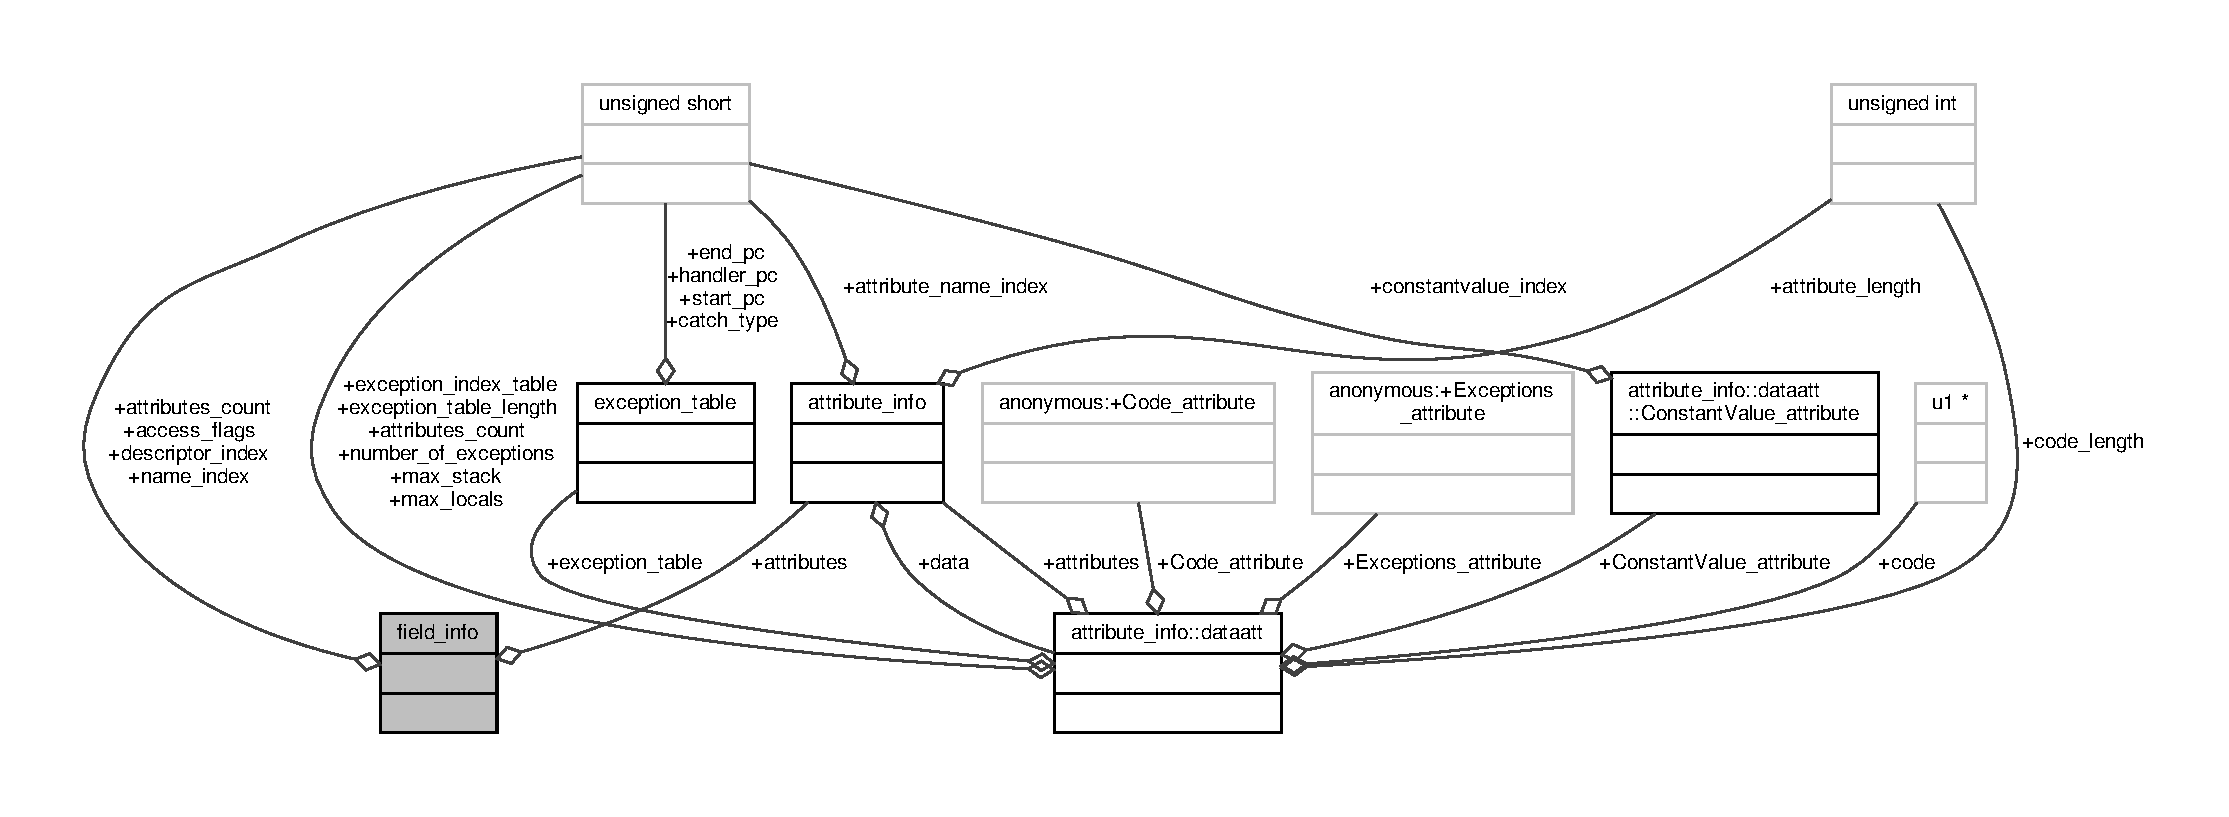
\includegraphics[width=350pt]{structfield__info__coll__graph}
\end{center}
\end{figure}
\subsection*{Atributos Públicos}
\begin{DoxyCompactItemize}
\item 
\hyperlink{ClassLoader_8h_a5f223212eef04d10a4550ded680cb1cf}{u2} \hyperlink{structfield__info_aa622dc9a5b5353d2f3eb2f416dacab4b}{access\+\_\+flags}
\item 
\hyperlink{ClassLoader_8h_a5f223212eef04d10a4550ded680cb1cf}{u2} \hyperlink{structfield__info_a425e3ae85badd81c67ef00acca85ad9e}{name\+\_\+index}
\item 
\hyperlink{ClassLoader_8h_a5f223212eef04d10a4550ded680cb1cf}{u2} \hyperlink{structfield__info_a12dd492b7fb1d61da1ac14938d97b07f}{descriptor\+\_\+index}
\item 
\hyperlink{ClassLoader_8h_a5f223212eef04d10a4550ded680cb1cf}{u2} \hyperlink{structfield__info_a83bfa4ff84a608e3dbd1c3968ebe1b80}{attributes\+\_\+count}
\item 
\hyperlink{structattribute__info}{attribute\+\_\+info} $\ast$ \hyperlink{structfield__info_afdda114944ae5eaae78c237f99257108}{attributes}
\end{DoxyCompactItemize}


\subsection{Descrição Detalhada}
Escrutura para gernciar as informações dos campos. 

\subsection{Atributos}
\mbox{\Hypertarget{structfield__info_aa622dc9a5b5353d2f3eb2f416dacab4b}\label{structfield__info_aa622dc9a5b5353d2f3eb2f416dacab4b}} 
\index{field\+\_\+info@{field\+\_\+info}!access\+\_\+flags@{access\+\_\+flags}}
\index{access\+\_\+flags@{access\+\_\+flags}!field\+\_\+info@{field\+\_\+info}}
\subsubsection{\texorpdfstring{access\+\_\+flags}{access\_flags}}
{\footnotesize\ttfamily \hyperlink{ClassLoader_8h_a5f223212eef04d10a4550ded680cb1cf}{u2} field\+\_\+info\+::access\+\_\+flags}

\mbox{\Hypertarget{structfield__info_afdda114944ae5eaae78c237f99257108}\label{structfield__info_afdda114944ae5eaae78c237f99257108}} 
\index{field\+\_\+info@{field\+\_\+info}!attributes@{attributes}}
\index{attributes@{attributes}!field\+\_\+info@{field\+\_\+info}}
\subsubsection{\texorpdfstring{attributes}{attributes}}
{\footnotesize\ttfamily \hyperlink{structattribute__info}{attribute\+\_\+info}$\ast$ field\+\_\+info\+::attributes}

\mbox{\Hypertarget{structfield__info_a83bfa4ff84a608e3dbd1c3968ebe1b80}\label{structfield__info_a83bfa4ff84a608e3dbd1c3968ebe1b80}} 
\index{field\+\_\+info@{field\+\_\+info}!attributes\+\_\+count@{attributes\+\_\+count}}
\index{attributes\+\_\+count@{attributes\+\_\+count}!field\+\_\+info@{field\+\_\+info}}
\subsubsection{\texorpdfstring{attributes\+\_\+count}{attributes\_count}}
{\footnotesize\ttfamily \hyperlink{ClassLoader_8h_a5f223212eef04d10a4550ded680cb1cf}{u2} field\+\_\+info\+::attributes\+\_\+count}

\mbox{\Hypertarget{structfield__info_a12dd492b7fb1d61da1ac14938d97b07f}\label{structfield__info_a12dd492b7fb1d61da1ac14938d97b07f}} 
\index{field\+\_\+info@{field\+\_\+info}!descriptor\+\_\+index@{descriptor\+\_\+index}}
\index{descriptor\+\_\+index@{descriptor\+\_\+index}!field\+\_\+info@{field\+\_\+info}}
\subsubsection{\texorpdfstring{descriptor\+\_\+index}{descriptor\_index}}
{\footnotesize\ttfamily \hyperlink{ClassLoader_8h_a5f223212eef04d10a4550ded680cb1cf}{u2} field\+\_\+info\+::descriptor\+\_\+index}

\mbox{\Hypertarget{structfield__info_a425e3ae85badd81c67ef00acca85ad9e}\label{structfield__info_a425e3ae85badd81c67ef00acca85ad9e}} 
\index{field\+\_\+info@{field\+\_\+info}!name\+\_\+index@{name\+\_\+index}}
\index{name\+\_\+index@{name\+\_\+index}!field\+\_\+info@{field\+\_\+info}}
\subsubsection{\texorpdfstring{name\+\_\+index}{name\_index}}
{\footnotesize\ttfamily \hyperlink{ClassLoader_8h_a5f223212eef04d10a4550ded680cb1cf}{u2} field\+\_\+info\+::name\+\_\+index}



A documentação para esta estrutura foi gerada a partir do seguinte arquivo\+:\begin{DoxyCompactItemize}
\item 
\hyperlink{ClassLoader_8h}{Class\+Loader.\+h}\end{DoxyCompactItemize}

\hypertarget{structframe}{}\section{Referência da Estrutura frame}
\label{structframe}\index{frame@{frame}}


Estrutura dos elementos da pilha de frames.  




{\ttfamily \#include $<$Frame\+Stack.\+h$>$}



Diagrama de colaboração para frame\+:
\nopagebreak
\begin{figure}[H]
\begin{center}
\leavevmode
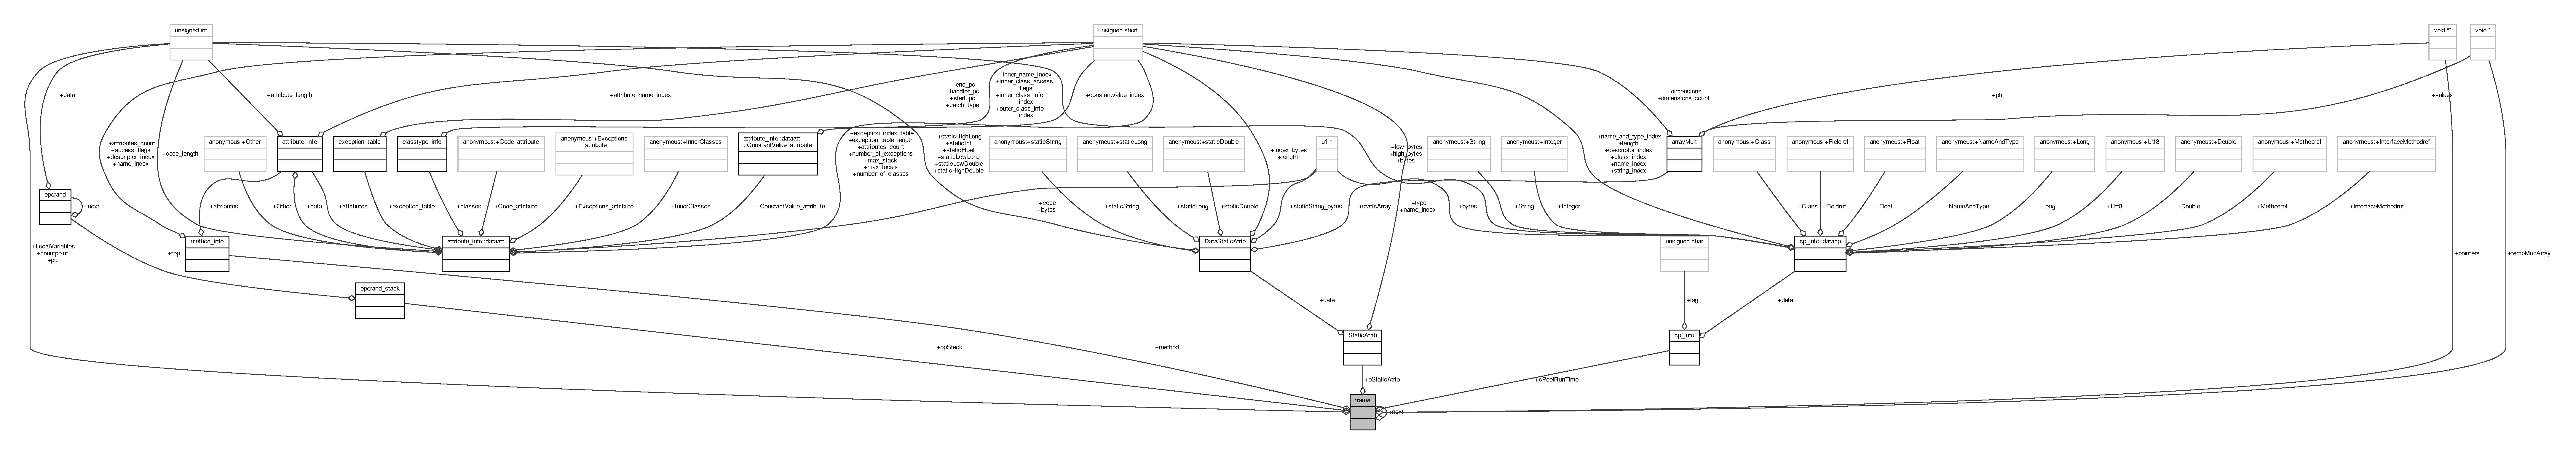
\includegraphics[width=350pt]{structframe__coll__graph}
\end{center}
\end{figure}
\subsection*{Atributos Públicos}
\begin{DoxyCompactItemize}
\item 
\hyperlink{structoperand__stack}{operand\+\_\+stack} \hyperlink{structframe_ac87e8a50c7f6d37600c44c1faca0f530}{op\+Stack}
\item 
\hyperlink{structcp__info}{cp\+\_\+info} $\ast$ \hyperlink{structframe_af9ce330bb6f6e4d7b2a5fb046f08e4dc}{c\+Pool\+Run\+Time}
\item 
\hyperlink{structStaticAtrib}{Static\+Atrib} $\ast$ \hyperlink{structframe_adf21113594c388521fe0f3591241f597}{p\+Static\+Atrib}
\item 
\hyperlink{ClassLoader_8h_aedf6ddc03df8caaaccbb4c60b9a9b850}{u4} $\ast$ \hyperlink{structframe_a1c91e0ecde5fe1fee5bf295f096b511f}{Local\+Variables}
\item 
void $\ast$$\ast$ \hyperlink{structframe_a29911524013a45af719b6d19592dc60d}{pointers}
\item 
\hyperlink{ClassLoader_8h_aedf6ddc03df8caaaccbb4c60b9a9b850}{u4} \hyperlink{structframe_aa4ce8c8307208f3fdf27b5a81fc265af}{countpoint}
\item 
void $\ast$ \hyperlink{structframe_ae25d34f063809e9990a1279fa9a794f4}{temp\+Mult\+Array}
\item 
\hyperlink{structmethod__info}{method\+\_\+info} $\ast$ \hyperlink{structframe_a2fac8190b89a1cf94c23628f1849a939}{method}
\item 
\hyperlink{ClassLoader_8h_aedf6ddc03df8caaaccbb4c60b9a9b850}{u4} \hyperlink{structframe_ae2f8c8d0abb0ff0952fb8ab971c2d3d0}{pc}
\item 
struct \hyperlink{structframe}{frame} $\ast$ \hyperlink{structframe_a23c908c0892e1329c82f3673e1d659eb}{next}
\end{DoxyCompactItemize}


\subsection{Descrição Detalhada}
Estrutura dos elementos da pilha de frames. 

\subsection{Atributos}
\mbox{\Hypertarget{structframe_aa4ce8c8307208f3fdf27b5a81fc265af}\label{structframe_aa4ce8c8307208f3fdf27b5a81fc265af}} 
\index{frame@{frame}!countpoint@{countpoint}}
\index{countpoint@{countpoint}!frame@{frame}}
\subsubsection{\texorpdfstring{countpoint}{countpoint}}
{\footnotesize\ttfamily \hyperlink{ClassLoader_8h_aedf6ddc03df8caaaccbb4c60b9a9b850}{u4} frame\+::countpoint}

\mbox{\Hypertarget{structframe_af9ce330bb6f6e4d7b2a5fb046f08e4dc}\label{structframe_af9ce330bb6f6e4d7b2a5fb046f08e4dc}} 
\index{frame@{frame}!c\+Pool\+Run\+Time@{c\+Pool\+Run\+Time}}
\index{c\+Pool\+Run\+Time@{c\+Pool\+Run\+Time}!frame@{frame}}
\subsubsection{\texorpdfstring{c\+Pool\+Run\+Time}{cPoolRunTime}}
{\footnotesize\ttfamily \hyperlink{structcp__info}{cp\+\_\+info}$\ast$ frame\+::c\+Pool\+Run\+Time}

\mbox{\Hypertarget{structframe_a1c91e0ecde5fe1fee5bf295f096b511f}\label{structframe_a1c91e0ecde5fe1fee5bf295f096b511f}} 
\index{frame@{frame}!Local\+Variables@{Local\+Variables}}
\index{Local\+Variables@{Local\+Variables}!frame@{frame}}
\subsubsection{\texorpdfstring{Local\+Variables}{LocalVariables}}
{\footnotesize\ttfamily \hyperlink{ClassLoader_8h_aedf6ddc03df8caaaccbb4c60b9a9b850}{u4}$\ast$ frame\+::\+Local\+Variables}

\mbox{\Hypertarget{structframe_a2fac8190b89a1cf94c23628f1849a939}\label{structframe_a2fac8190b89a1cf94c23628f1849a939}} 
\index{frame@{frame}!method@{method}}
\index{method@{method}!frame@{frame}}
\subsubsection{\texorpdfstring{method}{method}}
{\footnotesize\ttfamily \hyperlink{structmethod__info}{method\+\_\+info}$\ast$ frame\+::method}

\mbox{\Hypertarget{structframe_a23c908c0892e1329c82f3673e1d659eb}\label{structframe_a23c908c0892e1329c82f3673e1d659eb}} 
\index{frame@{frame}!next@{next}}
\index{next@{next}!frame@{frame}}
\subsubsection{\texorpdfstring{next}{next}}
{\footnotesize\ttfamily struct \hyperlink{structframe}{frame}$\ast$ frame\+::next}

\mbox{\Hypertarget{structframe_ac87e8a50c7f6d37600c44c1faca0f530}\label{structframe_ac87e8a50c7f6d37600c44c1faca0f530}} 
\index{frame@{frame}!op\+Stack@{op\+Stack}}
\index{op\+Stack@{op\+Stack}!frame@{frame}}
\subsubsection{\texorpdfstring{op\+Stack}{opStack}}
{\footnotesize\ttfamily \hyperlink{structoperand__stack}{operand\+\_\+stack} frame\+::op\+Stack}

\mbox{\Hypertarget{structframe_ae2f8c8d0abb0ff0952fb8ab971c2d3d0}\label{structframe_ae2f8c8d0abb0ff0952fb8ab971c2d3d0}} 
\index{frame@{frame}!pc@{pc}}
\index{pc@{pc}!frame@{frame}}
\subsubsection{\texorpdfstring{pc}{pc}}
{\footnotesize\ttfamily \hyperlink{ClassLoader_8h_aedf6ddc03df8caaaccbb4c60b9a9b850}{u4} frame\+::pc}

\mbox{\Hypertarget{structframe_a29911524013a45af719b6d19592dc60d}\label{structframe_a29911524013a45af719b6d19592dc60d}} 
\index{frame@{frame}!pointers@{pointers}}
\index{pointers@{pointers}!frame@{frame}}
\subsubsection{\texorpdfstring{pointers}{pointers}}
{\footnotesize\ttfamily void$\ast$$\ast$ frame\+::pointers}

\mbox{\Hypertarget{structframe_adf21113594c388521fe0f3591241f597}\label{structframe_adf21113594c388521fe0f3591241f597}} 
\index{frame@{frame}!p\+Static\+Atrib@{p\+Static\+Atrib}}
\index{p\+Static\+Atrib@{p\+Static\+Atrib}!frame@{frame}}
\subsubsection{\texorpdfstring{p\+Static\+Atrib}{pStaticAtrib}}
{\footnotesize\ttfamily \hyperlink{structStaticAtrib}{Static\+Atrib}$\ast$ frame\+::p\+Static\+Atrib}

\mbox{\Hypertarget{structframe_ae25d34f063809e9990a1279fa9a794f4}\label{structframe_ae25d34f063809e9990a1279fa9a794f4}} 
\index{frame@{frame}!temp\+Mult\+Array@{temp\+Mult\+Array}}
\index{temp\+Mult\+Array@{temp\+Mult\+Array}!frame@{frame}}
\subsubsection{\texorpdfstring{temp\+Mult\+Array}{tempMultArray}}
{\footnotesize\ttfamily void$\ast$ frame\+::temp\+Mult\+Array}



A documentação para esta estrutura foi gerada a partir do seguinte arquivo\+:\begin{DoxyCompactItemize}
\item 
\hyperlink{FrameStack_8h}{Frame\+Stack.\+h}\end{DoxyCompactItemize}

\hypertarget{structFrameStack}{}\section{Referência da Estrutura Frame\+Stack}
\label{structFrameStack}\index{Frame\+Stack@{Frame\+Stack}}


Estrutura da pilha de frames.  




{\ttfamily \#include $<$Frame\+Stack.\+h$>$}



Diagrama de colaboração para Frame\+Stack\+:
\nopagebreak
\begin{figure}[H]
\begin{center}
\leavevmode
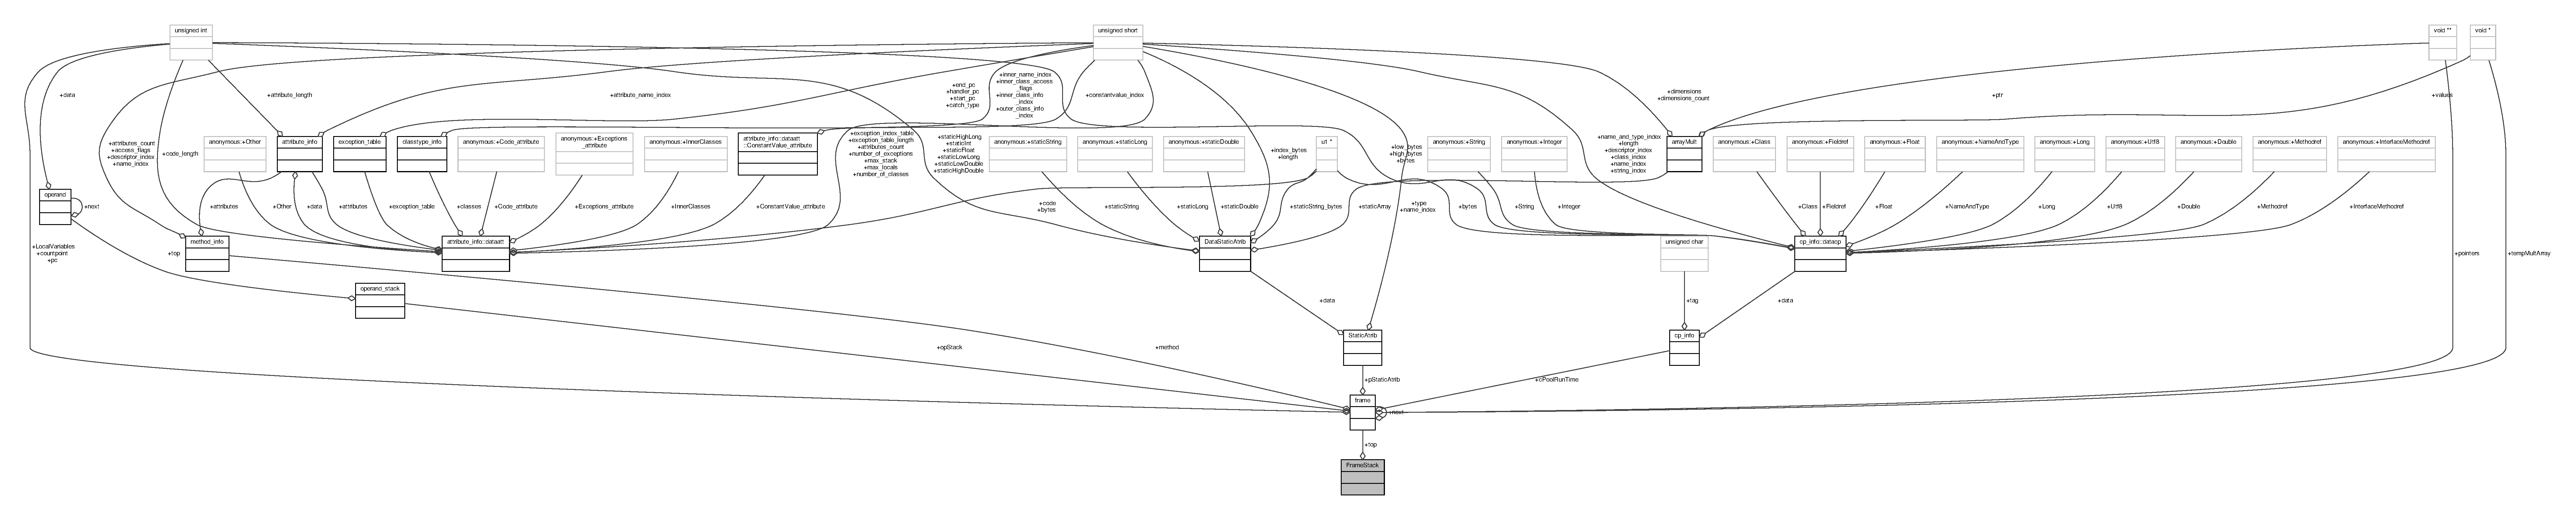
\includegraphics[width=350pt]{structFrameStack__coll__graph}
\end{center}
\end{figure}
\subsection*{Atributos Públicos}
\begin{DoxyCompactItemize}
\item 
struct \hyperlink{structframe}{frame} $\ast$ \hyperlink{structFrameStack_a0b30458d8eb5565c6fa8db0cb4b4bebd}{top}
\end{DoxyCompactItemize}


\subsection{Descrição Detalhada}
Estrutura da pilha de frames. 

\subsection{Atributos}
\mbox{\Hypertarget{structFrameStack_a0b30458d8eb5565c6fa8db0cb4b4bebd}\label{structFrameStack_a0b30458d8eb5565c6fa8db0cb4b4bebd}} 
\index{Frame\+Stack@{Frame\+Stack}!top@{top}}
\index{top@{top}!Frame\+Stack@{Frame\+Stack}}
\subsubsection{\texorpdfstring{top}{top}}
{\footnotesize\ttfamily struct \hyperlink{structframe}{frame}$\ast$ Frame\+Stack\+::top}



A documentação para esta estrutura foi gerada a partir do seguinte arquivo\+:\begin{DoxyCompactItemize}
\item 
\hyperlink{FrameStack_8h}{Frame\+Stack.\+h}\end{DoxyCompactItemize}

\hypertarget{structmethod__info}{}\section{Referência da Estrutura method\+\_\+info}
\label{structmethod__info}\index{method\+\_\+info@{method\+\_\+info}}


Escrutura para gernciar as informações dos metodos.  




{\ttfamily \#include $<$Class\+Loader.\+h$>$}



Diagrama de colaboração para method\+\_\+info\+:
\nopagebreak
\begin{figure}[H]
\begin{center}
\leavevmode
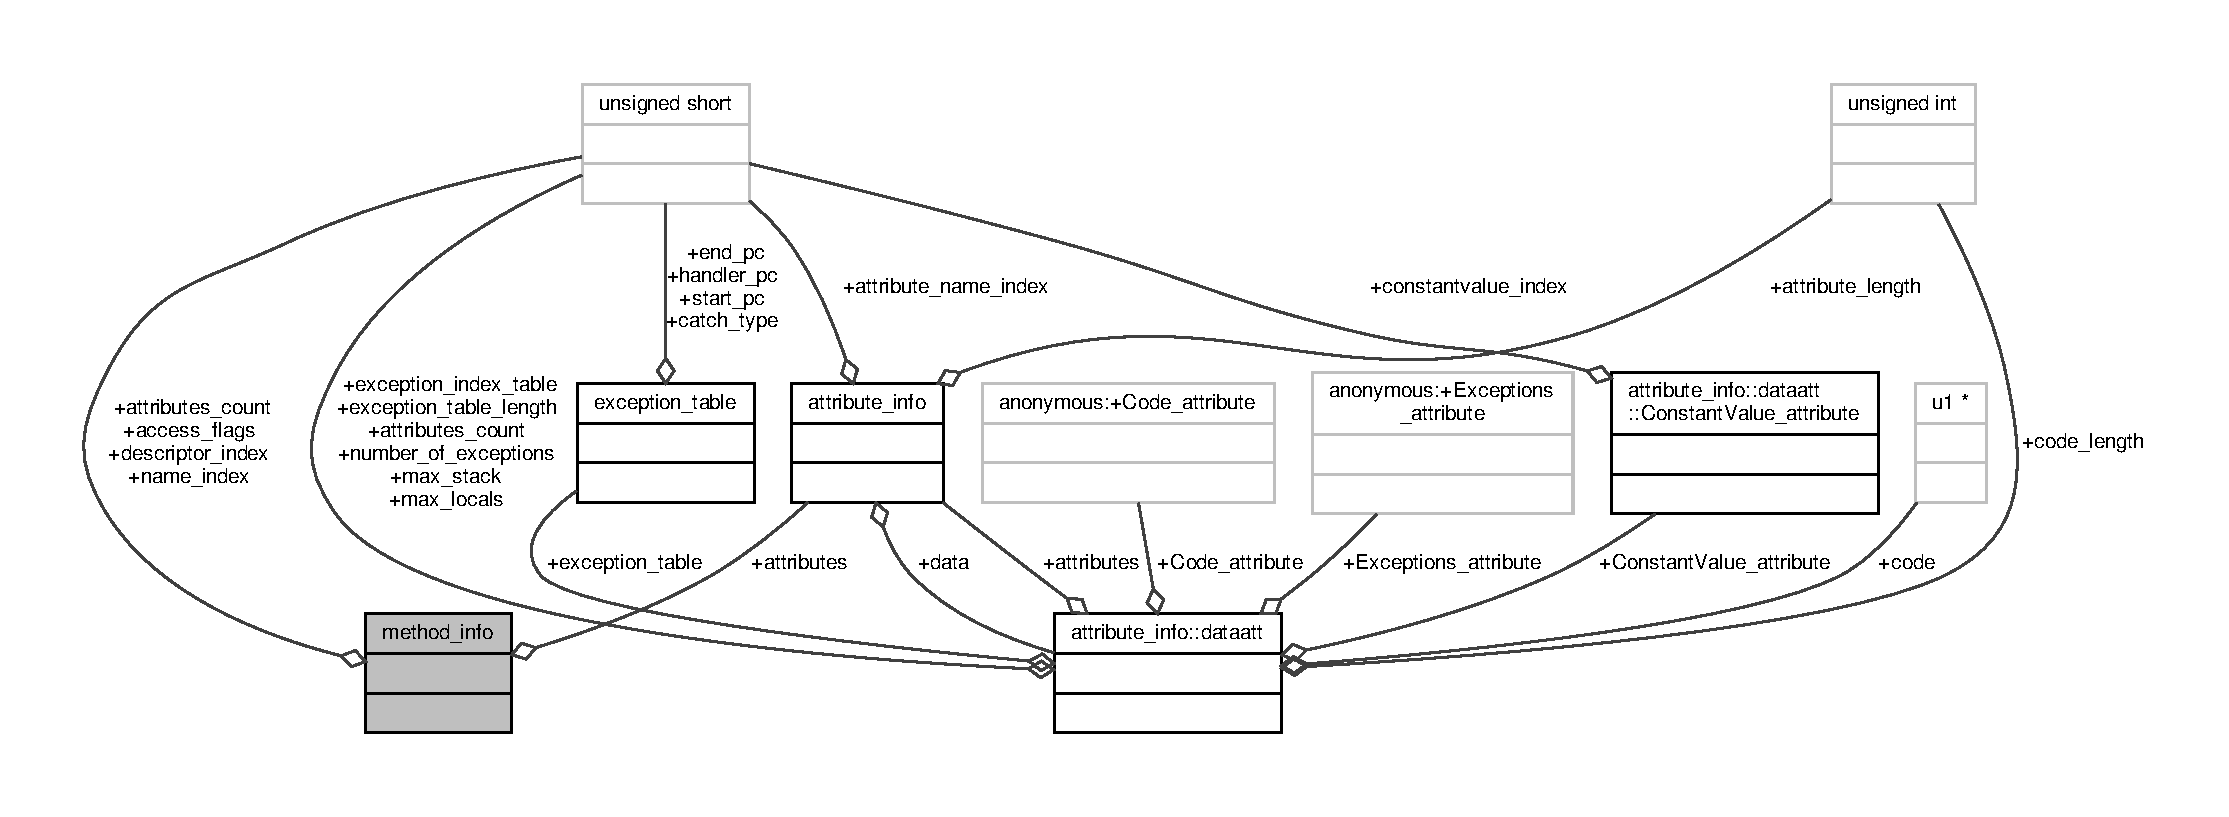
\includegraphics[width=350pt]{structmethod__info__coll__graph}
\end{center}
\end{figure}
\subsection*{Atributos Públicos}
\begin{DoxyCompactItemize}
\item 
\hyperlink{ClassLoader_8h_a5f223212eef04d10a4550ded680cb1cf}{u2} \hyperlink{structmethod__info_a3b657027a141cdbc94ded28607c98be5}{access\+\_\+flags}
\item 
\hyperlink{ClassLoader_8h_a5f223212eef04d10a4550ded680cb1cf}{u2} \hyperlink{structmethod__info_ab91d62d0658b77bba83f6bb685e3bbb9}{name\+\_\+index}
\item 
\hyperlink{ClassLoader_8h_a5f223212eef04d10a4550ded680cb1cf}{u2} \hyperlink{structmethod__info_a7713103e0c8d060630ad62774fb9be37}{descriptor\+\_\+index}
\item 
\hyperlink{ClassLoader_8h_a5f223212eef04d10a4550ded680cb1cf}{u2} \hyperlink{structmethod__info_ad9e5e1e2fc850806addadd6deab8565d}{attributes\+\_\+count}
\item 
\hyperlink{structattribute__info}{attribute\+\_\+info} $\ast$ \hyperlink{structmethod__info_a8ce4caaa03680c91f548558a38647ad8}{attributes}
\end{DoxyCompactItemize}


\subsection{Descrição Detalhada}
Escrutura para gernciar as informações dos metodos. 

\subsection{Atributos}
\mbox{\Hypertarget{structmethod__info_a3b657027a141cdbc94ded28607c98be5}\label{structmethod__info_a3b657027a141cdbc94ded28607c98be5}} 
\index{method\+\_\+info@{method\+\_\+info}!access\+\_\+flags@{access\+\_\+flags}}
\index{access\+\_\+flags@{access\+\_\+flags}!method\+\_\+info@{method\+\_\+info}}
\subsubsection{\texorpdfstring{access\+\_\+flags}{access\_flags}}
{\footnotesize\ttfamily \hyperlink{ClassLoader_8h_a5f223212eef04d10a4550ded680cb1cf}{u2} method\+\_\+info\+::access\+\_\+flags}

\mbox{\Hypertarget{structmethod__info_a8ce4caaa03680c91f548558a38647ad8}\label{structmethod__info_a8ce4caaa03680c91f548558a38647ad8}} 
\index{method\+\_\+info@{method\+\_\+info}!attributes@{attributes}}
\index{attributes@{attributes}!method\+\_\+info@{method\+\_\+info}}
\subsubsection{\texorpdfstring{attributes}{attributes}}
{\footnotesize\ttfamily \hyperlink{structattribute__info}{attribute\+\_\+info}$\ast$ method\+\_\+info\+::attributes}

\mbox{\Hypertarget{structmethod__info_ad9e5e1e2fc850806addadd6deab8565d}\label{structmethod__info_ad9e5e1e2fc850806addadd6deab8565d}} 
\index{method\+\_\+info@{method\+\_\+info}!attributes\+\_\+count@{attributes\+\_\+count}}
\index{attributes\+\_\+count@{attributes\+\_\+count}!method\+\_\+info@{method\+\_\+info}}
\subsubsection{\texorpdfstring{attributes\+\_\+count}{attributes\_count}}
{\footnotesize\ttfamily \hyperlink{ClassLoader_8h_a5f223212eef04d10a4550ded680cb1cf}{u2} method\+\_\+info\+::attributes\+\_\+count}

\mbox{\Hypertarget{structmethod__info_a7713103e0c8d060630ad62774fb9be37}\label{structmethod__info_a7713103e0c8d060630ad62774fb9be37}} 
\index{method\+\_\+info@{method\+\_\+info}!descriptor\+\_\+index@{descriptor\+\_\+index}}
\index{descriptor\+\_\+index@{descriptor\+\_\+index}!method\+\_\+info@{method\+\_\+info}}
\subsubsection{\texorpdfstring{descriptor\+\_\+index}{descriptor\_index}}
{\footnotesize\ttfamily \hyperlink{ClassLoader_8h_a5f223212eef04d10a4550ded680cb1cf}{u2} method\+\_\+info\+::descriptor\+\_\+index}

\mbox{\Hypertarget{structmethod__info_ab91d62d0658b77bba83f6bb685e3bbb9}\label{structmethod__info_ab91d62d0658b77bba83f6bb685e3bbb9}} 
\index{method\+\_\+info@{method\+\_\+info}!name\+\_\+index@{name\+\_\+index}}
\index{name\+\_\+index@{name\+\_\+index}!method\+\_\+info@{method\+\_\+info}}
\subsubsection{\texorpdfstring{name\+\_\+index}{name\_index}}
{\footnotesize\ttfamily \hyperlink{ClassLoader_8h_a5f223212eef04d10a4550ded680cb1cf}{u2} method\+\_\+info\+::name\+\_\+index}



A documentação para esta estrutura foi gerada a partir do seguinte arquivo\+:\begin{DoxyCompactItemize}
\item 
\hyperlink{ClassLoader_8h}{Class\+Loader.\+h}\end{DoxyCompactItemize}

\hypertarget{structObject}{}\section{Referência da Estrutura Object}
\label{structObject}\index{Object@{Object}}


Estrutura que gerencia os atributos dinâmicos, mais geral.  




{\ttfamily \#include $<$Method\+Area.\+h$>$}



Diagrama de colaboração para Object\+:
\nopagebreak
\begin{figure}[H]
\begin{center}
\leavevmode
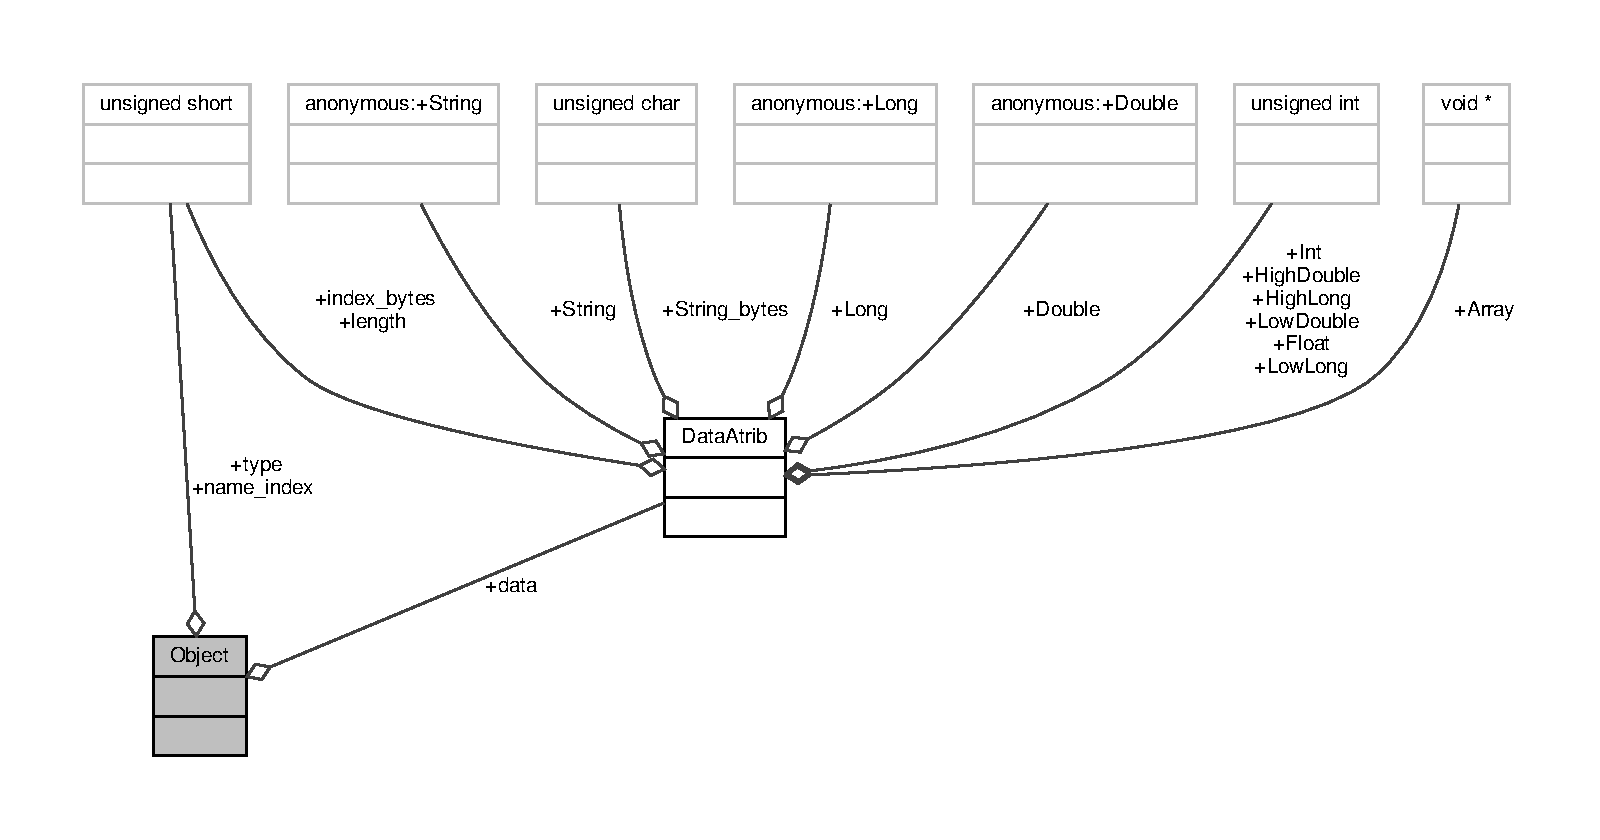
\includegraphics[width=350pt]{structObject__coll__graph}
\end{center}
\end{figure}
\subsection*{Atributos Públicos}
\begin{DoxyCompactItemize}
\item 
\hyperlink{ClassLoader_8h_a5f223212eef04d10a4550ded680cb1cf}{u2} \hyperlink{structObject_a0d3800016b59f53a98979f1c05a166f6}{type}
\item 
\hyperlink{ClassLoader_8h_a5f223212eef04d10a4550ded680cb1cf}{u2} \hyperlink{structObject_a792741be5e389dce8261c75ada556006}{name\+\_\+index}
\item 
\hyperlink{unionDataAtrib}{Data\+Atrib} \hyperlink{structObject_aea3a2d0f5d67e5b8e9259f02f2b744da}{data}
\end{DoxyCompactItemize}


\subsection{Descrição Detalhada}
Estrutura que gerencia os atributos dinâmicos, mais geral. 

\subsection{Atributos}
\mbox{\Hypertarget{structObject_aea3a2d0f5d67e5b8e9259f02f2b744da}\label{structObject_aea3a2d0f5d67e5b8e9259f02f2b744da}} 
\index{Object@{Object}!data@{data}}
\index{data@{data}!Object@{Object}}
\subsubsection{\texorpdfstring{data}{data}}
{\footnotesize\ttfamily \hyperlink{unionDataAtrib}{Data\+Atrib} Object\+::data}

\mbox{\Hypertarget{structObject_a792741be5e389dce8261c75ada556006}\label{structObject_a792741be5e389dce8261c75ada556006}} 
\index{Object@{Object}!name\+\_\+index@{name\+\_\+index}}
\index{name\+\_\+index@{name\+\_\+index}!Object@{Object}}
\subsubsection{\texorpdfstring{name\+\_\+index}{name\_index}}
{\footnotesize\ttfamily \hyperlink{ClassLoader_8h_a5f223212eef04d10a4550ded680cb1cf}{u2} Object\+::name\+\_\+index}

\mbox{\Hypertarget{structObject_a0d3800016b59f53a98979f1c05a166f6}\label{structObject_a0d3800016b59f53a98979f1c05a166f6}} 
\index{Object@{Object}!type@{type}}
\index{type@{type}!Object@{Object}}
\subsubsection{\texorpdfstring{type}{type}}
{\footnotesize\ttfamily \hyperlink{ClassLoader_8h_a5f223212eef04d10a4550ded680cb1cf}{u2} Object\+::type}



A documentação para esta estrutura foi gerada a partir do seguinte arquivo\+:\begin{DoxyCompactItemize}
\item 
\hyperlink{MethodArea_8h}{Method\+Area.\+h}\end{DoxyCompactItemize}

\hypertarget{structoperand}{}\section{Referência da Estrutura operand}
\label{structoperand}\index{operand@{operand}}


{\ttfamily \#include $<$Frame\+Stack.\+h$>$}



Diagrama de colaboração para operand\+:\nopagebreak
\begin{figure}[H]
\begin{center}
\leavevmode
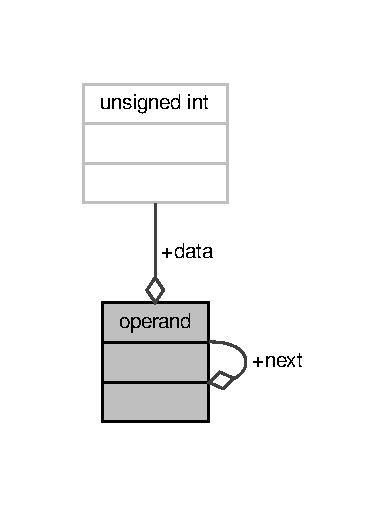
\includegraphics[width=186pt]{structoperand__coll__graph}
\end{center}
\end{figure}
\subsection*{Atributos Públicos}
\begin{DoxyCompactItemize}
\item 
\hyperlink{ClassLoader_8h_aedf6ddc03df8caaaccbb4c60b9a9b850}{u4} \hyperlink{structoperand_a837c1053ce4d46fe295fbbe0f16c25ff}{data}
\item 
struct \hyperlink{structoperand}{operand} $\ast$ \hyperlink{structoperand_abdf650090955fbf7cb74c6d8cbc12eef}{next}
\end{DoxyCompactItemize}


\subsection{Atributos}
\mbox{\Hypertarget{structoperand_a837c1053ce4d46fe295fbbe0f16c25ff}\label{structoperand_a837c1053ce4d46fe295fbbe0f16c25ff}} 
\index{operand@{operand}!data@{data}}
\index{data@{data}!operand@{operand}}
\subsubsection{\texorpdfstring{data}{data}}
{\footnotesize\ttfamily \hyperlink{ClassLoader_8h_aedf6ddc03df8caaaccbb4c60b9a9b850}{u4} operand\+::data}

\mbox{\Hypertarget{structoperand_abdf650090955fbf7cb74c6d8cbc12eef}\label{structoperand_abdf650090955fbf7cb74c6d8cbc12eef}} 
\index{operand@{operand}!next@{next}}
\index{next@{next}!operand@{operand}}
\subsubsection{\texorpdfstring{next}{next}}
{\footnotesize\ttfamily struct \hyperlink{structoperand}{operand}$\ast$ operand\+::next}



A documentação para esta estrutura foi gerada a partir do seguinte arquivo\+:\begin{DoxyCompactItemize}
\item 
\hyperlink{FrameStack_8h}{Frame\+Stack.\+h}\end{DoxyCompactItemize}

\hypertarget{structoperand__stack}{}\section{Referência da Estrutura operand\+\_\+stack}
\label{structoperand__stack}\index{operand\+\_\+stack@{operand\+\_\+stack}}


Estrutura da pilha propriamente dita.  




{\ttfamily \#include $<$Frame\+Stack.\+h$>$}



Diagrama de colaboração para operand\+\_\+stack\+:\nopagebreak
\begin{figure}[H]
\begin{center}
\leavevmode
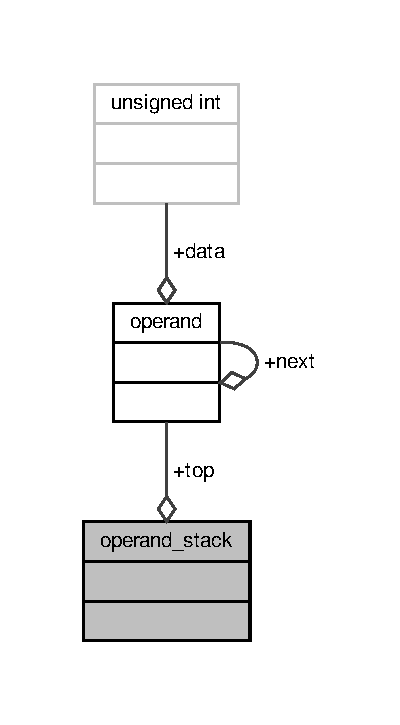
\includegraphics[width=192pt]{structoperand__stack__coll__graph}
\end{center}
\end{figure}
\subsection*{Atributos Públicos}
\begin{DoxyCompactItemize}
\item 
struct \hyperlink{structoperand}{operand} $\ast$ \hyperlink{structoperand__stack_a39f0f405579d0f45a1d03b30b1c2731e}{top}
\end{DoxyCompactItemize}


\subsection{Descrição Detalhada}
Estrutura da pilha propriamente dita. 

\subsection{Atributos}
\mbox{\Hypertarget{structoperand__stack_a39f0f405579d0f45a1d03b30b1c2731e}\label{structoperand__stack_a39f0f405579d0f45a1d03b30b1c2731e}} 
\index{operand\+\_\+stack@{operand\+\_\+stack}!top@{top}}
\index{top@{top}!operand\+\_\+stack@{operand\+\_\+stack}}
\subsubsection{\texorpdfstring{top}{top}}
{\footnotesize\ttfamily struct \hyperlink{structoperand}{operand}$\ast$ operand\+\_\+stack\+::top}



A documentação para esta estrutura foi gerada a partir do seguinte arquivo\+:\begin{DoxyCompactItemize}
\item 
\hyperlink{FrameStack_8h}{Frame\+Stack.\+h}\end{DoxyCompactItemize}

\hypertarget{structStaticAtrib}{}\section{Referência da Estrutura Static\+Atrib}
\label{structStaticAtrib}\index{Static\+Atrib@{Static\+Atrib}}


Estrutura que gerencia os atributos estáticos, mais geral.  




{\ttfamily \#include $<$Method\+Area.\+h$>$}



Diagrama de colaboração para Static\+Atrib\+:
\nopagebreak
\begin{figure}[H]
\begin{center}
\leavevmode
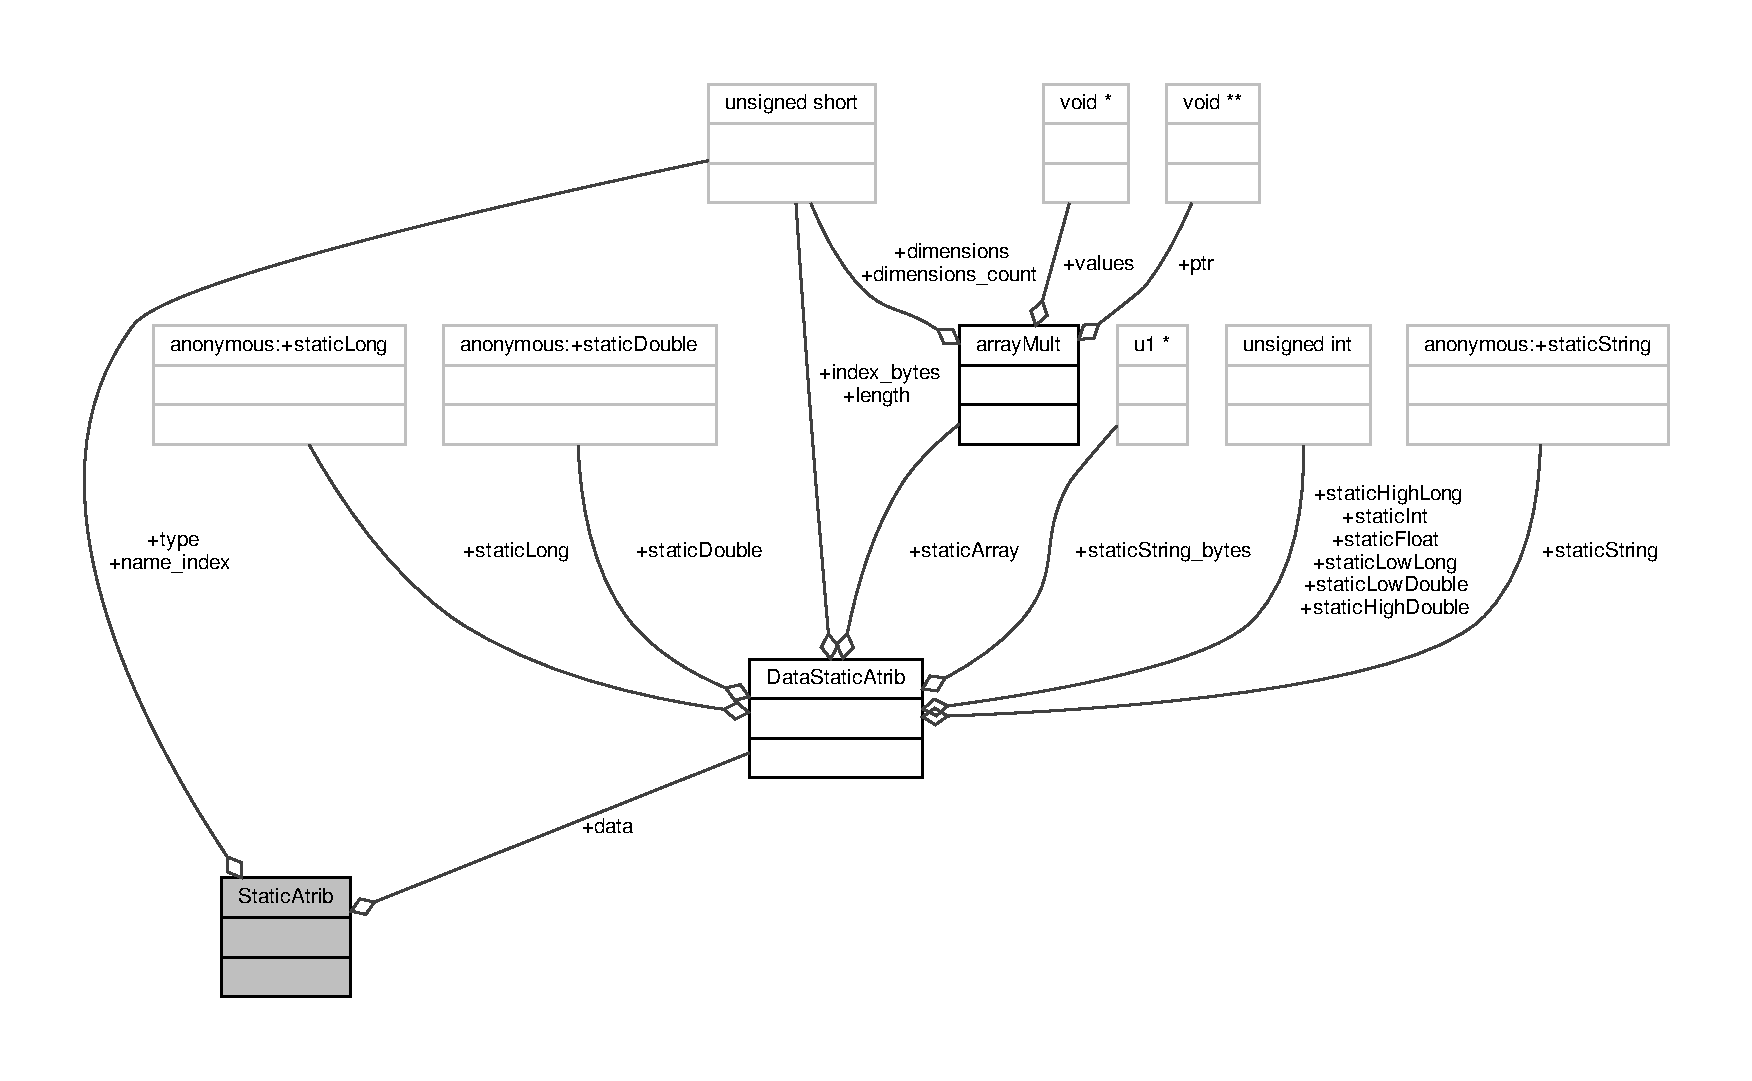
\includegraphics[width=350pt]{structStaticAtrib__coll__graph}
\end{center}
\end{figure}
\subsection*{Atributos Públicos}
\begin{DoxyCompactItemize}
\item 
\hyperlink{ClassLoader_8h_a5f223212eef04d10a4550ded680cb1cf}{u2} \hyperlink{structStaticAtrib_ace3f941daa9df10a76029562b3f9cef3}{type}
\item 
\hyperlink{ClassLoader_8h_a5f223212eef04d10a4550ded680cb1cf}{u2} \hyperlink{structStaticAtrib_a7066a25332e32a5d8eccc92d8b303635}{name\+\_\+index}
\item 
\hyperlink{unionDataStaticAtrib}{Data\+Static\+Atrib} \hyperlink{structStaticAtrib_aa9c612ef7f4696833d6658c21691b048}{data}
\end{DoxyCompactItemize}


\subsection{Descrição Detalhada}
Estrutura que gerencia os atributos estáticos, mais geral. 

\subsection{Atributos}
\mbox{\Hypertarget{structStaticAtrib_aa9c612ef7f4696833d6658c21691b048}\label{structStaticAtrib_aa9c612ef7f4696833d6658c21691b048}} 
\index{Static\+Atrib@{Static\+Atrib}!data@{data}}
\index{data@{data}!Static\+Atrib@{Static\+Atrib}}
\subsubsection{\texorpdfstring{data}{data}}
{\footnotesize\ttfamily \hyperlink{unionDataStaticAtrib}{Data\+Static\+Atrib} Static\+Atrib\+::data}

\mbox{\Hypertarget{structStaticAtrib_a7066a25332e32a5d8eccc92d8b303635}\label{structStaticAtrib_a7066a25332e32a5d8eccc92d8b303635}} 
\index{Static\+Atrib@{Static\+Atrib}!name\+\_\+index@{name\+\_\+index}}
\index{name\+\_\+index@{name\+\_\+index}!Static\+Atrib@{Static\+Atrib}}
\subsubsection{\texorpdfstring{name\+\_\+index}{name\_index}}
{\footnotesize\ttfamily \hyperlink{ClassLoader_8h_a5f223212eef04d10a4550ded680cb1cf}{u2} Static\+Atrib\+::name\+\_\+index}

\mbox{\Hypertarget{structStaticAtrib_ace3f941daa9df10a76029562b3f9cef3}\label{structStaticAtrib_ace3f941daa9df10a76029562b3f9cef3}} 
\index{Static\+Atrib@{Static\+Atrib}!type@{type}}
\index{type@{type}!Static\+Atrib@{Static\+Atrib}}
\subsubsection{\texorpdfstring{type}{type}}
{\footnotesize\ttfamily \hyperlink{ClassLoader_8h_a5f223212eef04d10a4550ded680cb1cf}{u2} Static\+Atrib\+::type}



A documentação para esta estrutura foi gerada a partir do seguinte arquivo\+:\begin{DoxyCompactItemize}
\item 
\hyperlink{MethodArea_8h}{Method\+Area.\+h}\end{DoxyCompactItemize}

\chapter{Arquivos}
\hypertarget{AuxiliarInstructions_8h}{}\section{Referência do Arquivo Auxiliar\+Instructions.\+h}
\label{AuxiliarInstructions_8h}\index{Auxiliar\+Instructions.\+h@{Auxiliar\+Instructions.\+h}}
{\ttfamily \#include \char`\"{}Class\+Loader.\+h\char`\"{}}\newline
Gráfico de dependência de inclusões para Auxiliar\+Instructions.\+h\+:
\nopagebreak
\begin{figure}[H]
\begin{center}
\leavevmode
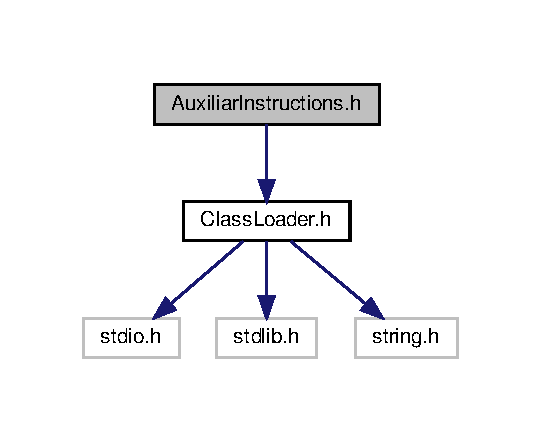
\includegraphics[width=260pt]{AuxiliarInstructions_8h__incl}
\end{center}
\end{figure}
Este grafo mostra quais arquivos estão direta ou indiretamente relacionados com este arquivo\+:
\nopagebreak
\begin{figure}[H]
\begin{center}
\leavevmode
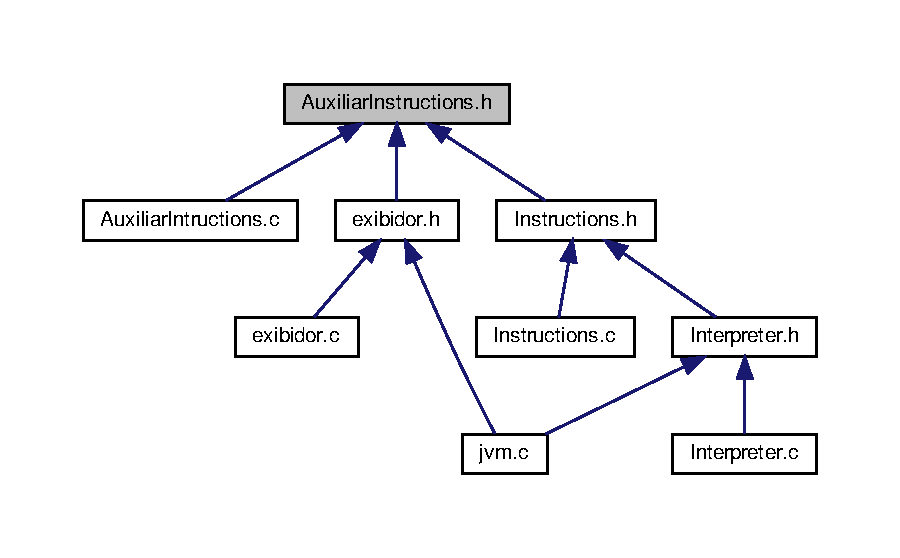
\includegraphics[width=350pt]{AuxiliarInstructions_8h__dep__incl}
\end{center}
\end{figure}
\subsection*{Funções}
\begin{DoxyCompactItemize}
\item 
double \hyperlink{AuxiliarInstructions_8h_a2ddf65184015919487e6f86cd09a2c0e}{fmod} (double d1, double d2)
\begin{DoxyCompactList}\small\item\em Fun��o que calcula o resto da divisao doubles ,d2 double. \end{DoxyCompactList}\item 
float \hyperlink{AuxiliarInstructions_8h_a47e12021659aced21f63769f135cdba6}{quociente} (float f1, float f2)
\begin{DoxyCompactList}\small\item\em Fun��o que calcula a divisao de dois floats. \end{DoxyCompactList}\item 
int \hyperlink{AuxiliarInstructions_8h_ae2662ad52a6e9edfc5606af54f78ea4b}{return\+\_\+type} (char $\ast$type)
\end{DoxyCompactItemize}


\subsection{Funções}
\mbox{\Hypertarget{AuxiliarInstructions_8h_a2ddf65184015919487e6f86cd09a2c0e}\label{AuxiliarInstructions_8h_a2ddf65184015919487e6f86cd09a2c0e}} 
\index{Auxiliar\+Instructions.\+h@{Auxiliar\+Instructions.\+h}!fmod@{fmod}}
\index{fmod@{fmod}!Auxiliar\+Instructions.\+h@{Auxiliar\+Instructions.\+h}}
\subsubsection{\texorpdfstring{fmod()}{fmod()}}
{\footnotesize\ttfamily double fmod (\begin{DoxyParamCaption}\item[{double}]{d1,  }\item[{double}]{d2 }\end{DoxyParamCaption})}



Fun��o que calcula o resto da divisao doubles ,d2 double. 

\begin{DoxyReturn}{Retorna}
o resto 
\end{DoxyReturn}
\mbox{\Hypertarget{AuxiliarInstructions_8h_a47e12021659aced21f63769f135cdba6}\label{AuxiliarInstructions_8h_a47e12021659aced21f63769f135cdba6}} 
\index{Auxiliar\+Instructions.\+h@{Auxiliar\+Instructions.\+h}!quociente@{quociente}}
\index{quociente@{quociente}!Auxiliar\+Instructions.\+h@{Auxiliar\+Instructions.\+h}}
\subsubsection{\texorpdfstring{quociente()}{quociente()}}
{\footnotesize\ttfamily float quociente (\begin{DoxyParamCaption}\item[{float}]{f1,  }\item[{float}]{f2 }\end{DoxyParamCaption})}



Fun��o que calcula a divisao de dois floats. 


\begin{DoxyParams}{Parâmetros}
{\em f1,f2} & float \\
\hline
\end{DoxyParams}
\begin{DoxyReturn}{Retorna}
quociente 
\end{DoxyReturn}
\mbox{\Hypertarget{AuxiliarInstructions_8h_ae2662ad52a6e9edfc5606af54f78ea4b}\label{AuxiliarInstructions_8h_ae2662ad52a6e9edfc5606af54f78ea4b}} 
\index{Auxiliar\+Instructions.\+h@{Auxiliar\+Instructions.\+h}!return\+\_\+type@{return\+\_\+type}}
\index{return\+\_\+type@{return\+\_\+type}!Auxiliar\+Instructions.\+h@{Auxiliar\+Instructions.\+h}}
\subsubsection{\texorpdfstring{return\+\_\+type()}{return\_type()}}
{\footnotesize\ttfamily int return\+\_\+type (\begin{DoxyParamCaption}\item[{char $\ast$}]{type }\end{DoxyParamCaption})}


\hypertarget{AuxiliarIntructions_8c}{}\section{Referência do Arquivo Auxiliar\+Intructions.\+c}
\label{AuxiliarIntructions_8c}\index{Auxiliar\+Intructions.\+c@{Auxiliar\+Intructions.\+c}}
{\ttfamily \#include \char`\"{}Auxiliar\+Instructions.\+h\char`\"{}}\newline
Gráfico de dependência de inclusões para Auxiliar\+Intructions.\+c\+:
\nopagebreak
\begin{figure}[H]
\begin{center}
\leavevmode
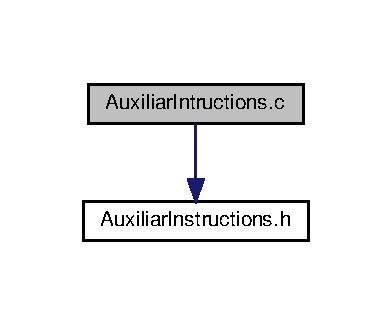
\includegraphics[width=260pt]{AuxiliarIntructions_8c__incl}
\end{center}
\end{figure}
\subsection*{Funções}
\begin{DoxyCompactItemize}
\item 
double \hyperlink{AuxiliarIntructions_8c_aa9b0019b802f303967c65472155f34f4}{fmod} (double f1, double f2)
\begin{DoxyCompactList}\small\item\em Fun��o que calcula o resto da divisao doubles ,d2 double. \end{DoxyCompactList}\item 
float \hyperlink{AuxiliarIntructions_8c_a47e12021659aced21f63769f135cdba6}{quociente} (float f1, float f2)
\begin{DoxyCompactList}\small\item\em Fun��o que calcula a divisao de dois floats. \end{DoxyCompactList}\item 
int \hyperlink{AuxiliarIntructions_8c_ae2662ad52a6e9edfc5606af54f78ea4b}{return\+\_\+type} (char $\ast$type)
\end{DoxyCompactItemize}


\subsection{Funções}
\mbox{\Hypertarget{AuxiliarIntructions_8c_aa9b0019b802f303967c65472155f34f4}\label{AuxiliarIntructions_8c_aa9b0019b802f303967c65472155f34f4}} 
\index{Auxiliar\+Intructions.\+c@{Auxiliar\+Intructions.\+c}!fmod@{fmod}}
\index{fmod@{fmod}!Auxiliar\+Intructions.\+c@{Auxiliar\+Intructions.\+c}}
\subsubsection{\texorpdfstring{fmod()}{fmod()}}
{\footnotesize\ttfamily double fmod (\begin{DoxyParamCaption}\item[{double}]{d1,  }\item[{double}]{d2 }\end{DoxyParamCaption})}



Fun��o que calcula o resto da divisao doubles ,d2 double. 

\begin{DoxyReturn}{Retorna}
o resto 
\end{DoxyReturn}
\mbox{\Hypertarget{AuxiliarIntructions_8c_a47e12021659aced21f63769f135cdba6}\label{AuxiliarIntructions_8c_a47e12021659aced21f63769f135cdba6}} 
\index{Auxiliar\+Intructions.\+c@{Auxiliar\+Intructions.\+c}!quociente@{quociente}}
\index{quociente@{quociente}!Auxiliar\+Intructions.\+c@{Auxiliar\+Intructions.\+c}}
\subsubsection{\texorpdfstring{quociente()}{quociente()}}
{\footnotesize\ttfamily float quociente (\begin{DoxyParamCaption}\item[{float}]{f1,  }\item[{float}]{f2 }\end{DoxyParamCaption})}



Fun��o que calcula a divisao de dois floats. 


\begin{DoxyParams}{Parâmetros}
{\em f1,f2} & float \\
\hline
\end{DoxyParams}
\begin{DoxyReturn}{Retorna}
quociente 
\end{DoxyReturn}
\mbox{\Hypertarget{AuxiliarIntructions_8c_ae2662ad52a6e9edfc5606af54f78ea4b}\label{AuxiliarIntructions_8c_ae2662ad52a6e9edfc5606af54f78ea4b}} 
\index{Auxiliar\+Intructions.\+c@{Auxiliar\+Intructions.\+c}!return\+\_\+type@{return\+\_\+type}}
\index{return\+\_\+type@{return\+\_\+type}!Auxiliar\+Intructions.\+c@{Auxiliar\+Intructions.\+c}}
\subsubsection{\texorpdfstring{return\+\_\+type()}{return\_type()}}
{\footnotesize\ttfamily int return\+\_\+type (\begin{DoxyParamCaption}\item[{char $\ast$}]{type }\end{DoxyParamCaption})}


\hypertarget{ClassLoader_8c}{}\section{Referência do Arquivo Class\+Loader.\+c}
\label{ClassLoader_8c}\index{Class\+Loader.\+c@{Class\+Loader.\+c}}
{\ttfamily \#include \char`\"{}Class\+Loader.\+h\char`\"{}}\newline
Gráfico de dependência de inclusões para Class\+Loader.\+c\+:\nopagebreak
\begin{figure}[H]
\begin{center}
\leavevmode
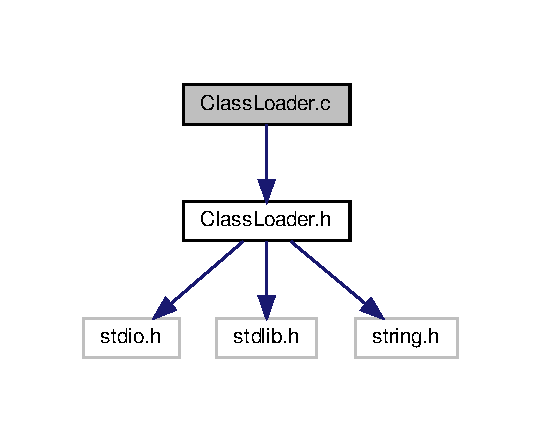
\includegraphics[width=260pt]{ClassLoader_8c__incl}
\end{center}
\end{figure}
\subsection*{Funções}
\begin{DoxyCompactItemize}
\item 
\hyperlink{ClassLoader_8h_a216a9f8b04b4f0af84a4ca9d1d85a6ca}{u1} \hyperlink{ClassLoader_8c_a77853ce0387c0b914b5a106ff7cf9ae9}{u1\+Read} (F\+I\+LE $\ast$fd)
\begin{DoxyCompactList}\small\item\em Função que le um byte do arquivo. \end{DoxyCompactList}\item 
\hyperlink{ClassLoader_8h_a5f223212eef04d10a4550ded680cb1cf}{u2} \hyperlink{ClassLoader_8c_a73788d4e3c1c3577021c1dbf4ca75cc1}{u2\+Read} (F\+I\+LE $\ast$fd)
\begin{DoxyCompactList}\small\item\em Função que le dois byte do arquivo. \end{DoxyCompactList}\item 
\hyperlink{ClassLoader_8h_aedf6ddc03df8caaaccbb4c60b9a9b850}{u4} \hyperlink{ClassLoader_8c_a4cba9f2733d339d7287d10d160c39e79}{u4\+Read} (F\+I\+LE $\ast$fd)
\begin{DoxyCompactList}\small\item\em Função que le quatro byte do arquivo. \end{DoxyCompactList}\item 
\hyperlink{structattribute__info}{attribute\+\_\+info} $\ast$ \hyperlink{ClassLoader_8c_aec485e0dbf4cf9a562e663eddf3835e1}{read\+\_\+attributes\+\_\+info} (\hyperlink{ClassLoader_8h_a5f223212eef04d10a4550ded680cb1cf}{u2} count, \hyperlink{structcp__info}{cp\+\_\+info} $\ast$cp, F\+I\+LE $\ast$ptr\+Class)
\item 
\hyperlink{structClassFile}{Class\+File} $\ast$ \hyperlink{ClassLoader_8c_a39d384ef8195b3711abd1c40b6fd5908}{read\+\_\+class} (char $\ast$filename)
\begin{DoxyCompactList}\small\item\em Função que le o bytecode java e monta a estrutura da classe. \end{DoxyCompactList}\end{DoxyCompactItemize}


\subsection{Funções}
\mbox{\Hypertarget{ClassLoader_8c_aec485e0dbf4cf9a562e663eddf3835e1}\label{ClassLoader_8c_aec485e0dbf4cf9a562e663eddf3835e1}} 
\index{Class\+Loader.\+c@{Class\+Loader.\+c}!read\+\_\+attributes\+\_\+info@{read\+\_\+attributes\+\_\+info}}
\index{read\+\_\+attributes\+\_\+info@{read\+\_\+attributes\+\_\+info}!Class\+Loader.\+c@{Class\+Loader.\+c}}
\subsubsection{\texorpdfstring{read\+\_\+attributes\+\_\+info()}{read\_attributes\_info()}}
{\footnotesize\ttfamily \hyperlink{structattribute__info}{attribute\+\_\+info}$\ast$ read\+\_\+attributes\+\_\+info (\begin{DoxyParamCaption}\item[{\hyperlink{ClassLoader_8h_a5f223212eef04d10a4550ded680cb1cf}{u2}}]{count,  }\item[{\hyperlink{structcp__info}{cp\+\_\+info} $\ast$}]{cp,  }\item[{F\+I\+LE $\ast$}]{ptr\+Class }\end{DoxyParamCaption})}

Funcao que le as informacoes dos atributos no bytecode count Numero de atributos $\ast$cp Ponteiro para o constant pool $\ast$ptr\+Class Ponteiro para o arquivo ptr\+Attributes ponteiro para vetor de atributos \mbox{\Hypertarget{ClassLoader_8c_a39d384ef8195b3711abd1c40b6fd5908}\label{ClassLoader_8c_a39d384ef8195b3711abd1c40b6fd5908}} 
\index{Class\+Loader.\+c@{Class\+Loader.\+c}!read\+\_\+class@{read\+\_\+class}}
\index{read\+\_\+class@{read\+\_\+class}!Class\+Loader.\+c@{Class\+Loader.\+c}}
\subsubsection{\texorpdfstring{read\+\_\+class()}{read\_class()}}
{\footnotesize\ttfamily \hyperlink{structClassFile}{Class\+File}$\ast$ read\+\_\+class (\begin{DoxyParamCaption}\item[{char $\ast$}]{filename }\end{DoxyParamCaption})}



Função que le o bytecode java e monta a estrutura da classe. 


\begin{DoxyParams}{Parâmetros}
{\em $\ast$filename} & Endereço do arquivo \\
\hline
\end{DoxyParams}
\begin{DoxyReturn}{Retorna}
estrutura da classe montada 
\end{DoxyReturn}
\mbox{\Hypertarget{ClassLoader_8c_a77853ce0387c0b914b5a106ff7cf9ae9}\label{ClassLoader_8c_a77853ce0387c0b914b5a106ff7cf9ae9}} 
\index{Class\+Loader.\+c@{Class\+Loader.\+c}!u1\+Read@{u1\+Read}}
\index{u1\+Read@{u1\+Read}!Class\+Loader.\+c@{Class\+Loader.\+c}}
\subsubsection{\texorpdfstring{u1\+Read()}{u1Read()}}
{\footnotesize\ttfamily \hyperlink{ClassLoader_8h_a216a9f8b04b4f0af84a4ca9d1d85a6ca}{u1} u1\+Read (\begin{DoxyParamCaption}\item[{F\+I\+LE $\ast$}]{fd }\end{DoxyParamCaption})}



Função que le um byte do arquivo. 


\begin{DoxyParams}{Parâmetros}
{\em $\ast$fd} & endereço do arquivo \\
\hline
\end{DoxyParams}
\begin{DoxyReturn}{Retorna}
byte lido 
\end{DoxyReturn}
\mbox{\Hypertarget{ClassLoader_8c_a73788d4e3c1c3577021c1dbf4ca75cc1}\label{ClassLoader_8c_a73788d4e3c1c3577021c1dbf4ca75cc1}} 
\index{Class\+Loader.\+c@{Class\+Loader.\+c}!u2\+Read@{u2\+Read}}
\index{u2\+Read@{u2\+Read}!Class\+Loader.\+c@{Class\+Loader.\+c}}
\subsubsection{\texorpdfstring{u2\+Read()}{u2Read()}}
{\footnotesize\ttfamily \hyperlink{ClassLoader_8h_a5f223212eef04d10a4550ded680cb1cf}{u2} u2\+Read (\begin{DoxyParamCaption}\item[{F\+I\+LE $\ast$}]{fd }\end{DoxyParamCaption})}



Função que le dois byte do arquivo. 


\begin{DoxyParams}{Parâmetros}
{\em $\ast$fd} & endereço do arquivo \\
\hline
\end{DoxyParams}
\begin{DoxyReturn}{Retorna}
bytes lidos 
\end{DoxyReturn}
\mbox{\Hypertarget{ClassLoader_8c_a4cba9f2733d339d7287d10d160c39e79}\label{ClassLoader_8c_a4cba9f2733d339d7287d10d160c39e79}} 
\index{Class\+Loader.\+c@{Class\+Loader.\+c}!u4\+Read@{u4\+Read}}
\index{u4\+Read@{u4\+Read}!Class\+Loader.\+c@{Class\+Loader.\+c}}
\subsubsection{\texorpdfstring{u4\+Read()}{u4Read()}}
{\footnotesize\ttfamily \hyperlink{ClassLoader_8h_aedf6ddc03df8caaaccbb4c60b9a9b850}{u4} u4\+Read (\begin{DoxyParamCaption}\item[{F\+I\+LE $\ast$}]{fd }\end{DoxyParamCaption})}



Função que le quatro byte do arquivo. 


\begin{DoxyParams}{Parâmetros}
{\em $\ast$fd} & endereço do arquivo \\
\hline
\end{DoxyParams}
\begin{DoxyReturn}{Retorna}
bytes lidos 
\end{DoxyReturn}

\hypertarget{ClassLoader_8h}{}\section{Referência do Arquivo Class\+Loader.\+h}
\label{ClassLoader_8h}\index{Class\+Loader.\+h@{Class\+Loader.\+h}}
{\ttfamily \#include $<$stdio.\+h$>$}\newline
{\ttfamily \#include $<$stdlib.\+h$>$}\newline
{\ttfamily \#include $<$string.\+h$>$}\newline
Gráfico de dependência de inclusões para Class\+Loader.\+h\+:\nopagebreak
\begin{figure}[H]
\begin{center}
\leavevmode
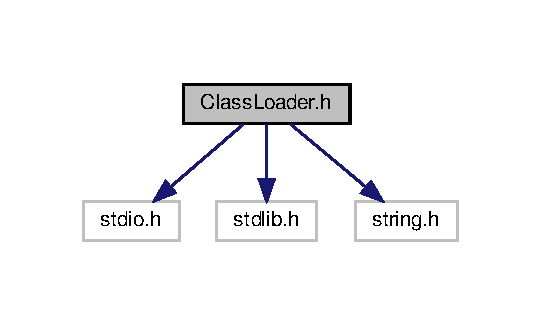
\includegraphics[width=260pt]{ClassLoader_8h__incl}
\end{center}
\end{figure}
Este grafo mostra quais arquivos estão direta ou indiretamente relacionados com este arquivo\+:\nopagebreak
\begin{figure}[H]
\begin{center}
\leavevmode
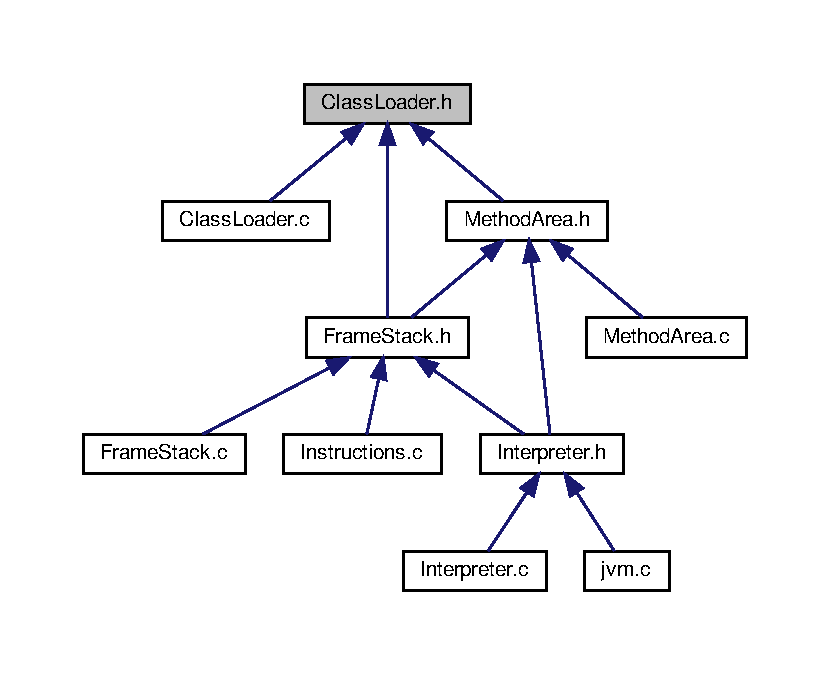
\includegraphics[width=350pt]{ClassLoader_8h__dep__incl}
\end{center}
\end{figure}
\subsection*{Componentes}
\begin{DoxyCompactItemize}
\item 
struct \hyperlink{structcp__info}{cp\+\_\+info}
\begin{DoxyCompactList}\small\item\em Estrutura do constant pool. \end{DoxyCompactList}\item 
union \hyperlink{unioncp__info_1_1datacp}{cp\+\_\+info\+::datacp}
\item 
struct \hyperlink{structexception__table}{exception\+\_\+table}
\begin{DoxyCompactList}\small\item\em Tabela de excesões. \end{DoxyCompactList}\item 
struct \hyperlink{structattribute__info}{attribute\+\_\+info}
\begin{DoxyCompactList}\small\item\em Estrutura das informações dos atributos. \end{DoxyCompactList}\item 
union \hyperlink{unionattribute__info_1_1dataatt}{attribute\+\_\+info\+::dataatt}
\item 
struct \hyperlink{structattribute__info_1_1dataatt_1_1ConstantValue__attribute}{attribute\+\_\+info\+::dataatt\+::\+Constant\+Value\+\_\+attribute}
\item 
struct \hyperlink{structfield__info}{field\+\_\+info}
\begin{DoxyCompactList}\small\item\em Escrutura para gernciar as informações dos campos. \end{DoxyCompactList}\item 
struct \hyperlink{structmethod__info}{method\+\_\+info}
\begin{DoxyCompactList}\small\item\em Escrutura para gernciar as informações dos metodos. \end{DoxyCompactList}\item 
struct \hyperlink{structClassFile}{Class\+File}
\begin{DoxyCompactList}\small\item\em Escrutura da classe. \end{DoxyCompactList}\end{DoxyCompactItemize}
\subsection*{Definições e Macros}
\begin{DoxyCompactItemize}
\item 
\#define \hyperlink{ClassLoader_8h_a3f5033dcfb4bfa9ee7e9de053bff97c2}{C\+L\+A\+S\+S\+\_\+\+I\+N\+D\+EX}~7
\item 
\#define \hyperlink{ClassLoader_8h_afbc7a63629d0bfdc607f8996f48bfb75}{F\+I\+E\+L\+D\+R\+EF}~9
\item 
\#define \hyperlink{ClassLoader_8h_a62bb4fccea133a58fd45b0ab68a2446f}{M\+E\+T\+H\+O\+D\+R\+EF}~10
\item 
\#define \hyperlink{ClassLoader_8h_a107c66129659d8570b334c27b4d32160}{I\+N\+T\+E\+R\+F\+A\+C\+E\+M\+E\+T\+H\+O\+D\+R\+EF}~11
\item 
\#define \hyperlink{ClassLoader_8h_a0f4d394a3ab4e09bff60f714c66dc5ee}{S\+T\+R\+I\+NG}~8
\item 
\#define \hyperlink{ClassLoader_8h_a91d43eadec33c80149f92e5abf5df58c}{I\+N\+T\+E\+G\+ER}~3
\item 
\#define \hyperlink{ClassLoader_8h_ae8690abbffa85934d64d545920e2b108}{F\+L\+O\+AT}~4
\item 
\#define \hyperlink{ClassLoader_8h_acaa7b8a7167a8214f499c71c413ddcca}{L\+O\+NG}~5
\item 
\#define \hyperlink{ClassLoader_8h_a8747af38b86aa2bbcda2f1b1aa0888c2}{D\+O\+U\+B\+LE}~6
\item 
\#define \hyperlink{ClassLoader_8h_ae7c13e0c35de16421035023bf9b8a914}{N\+A\+M\+E\+A\+N\+D\+T\+Y\+PE}~12
\item 
\#define \hyperlink{ClassLoader_8h_af9a8bd70343e082dbc63ac806b8ced24}{U\+T\+F8}~1
\item 
\#define \hyperlink{ClassLoader_8h_ae6527c8381eb3f23b7fd6d6efec6ffc7}{C\+O\+DE}~\char`\"{}Code\char`\"{}
\item 
\#define \hyperlink{ClassLoader_8h_a5e942d5b9cbcd72a52adaf04bb1dbf72}{C\+O\+N\+S\+T\+A\+N\+T\+\_\+\+V\+A\+L\+UE}~\char`\"{}Constant\+Value\char`\"{}
\item 
\#define \hyperlink{ClassLoader_8h_a4caa73a345f11f79bd729b3390c73427}{E\+X\+C\+E\+P\+T\+I\+O\+NS}~\char`\"{}Exceptions\char`\"{}
\item 
\#define \hyperlink{ClassLoader_8h_a53119d3081255979452287fd91342ab1}{R\+E\+F\+E\+R\+E\+N\+C\+E\+\_\+\+I\+N\+T\+E\+G\+ER}~15
\item 
\#define \hyperlink{ClassLoader_8h_a17e9a775a437ade11d6030fa3fb4e0c7}{R\+E\+F\+E\+R\+E\+N\+C\+E\+\_\+\+S\+T\+R\+I\+NG}~16
\item 
\#define \hyperlink{ClassLoader_8h_ac3b22f644fc7c1959775315d902f7dc2}{R\+E\+F\+E\+R\+E\+N\+C\+E\+\_\+\+F\+L\+O\+AT}~17
\item 
\#define \hyperlink{ClassLoader_8h_a153b8d56a11c980295ac1533dfe70028}{R\+E\+F\+E\+R\+E\+N\+C\+E\+\_\+\+L\+O\+NG}~18
\item 
\#define \hyperlink{ClassLoader_8h_a3d91751639ec82a19c99f8effae32152}{R\+E\+F\+E\+R\+E\+N\+C\+E\+\_\+\+D\+O\+U\+B\+LE}~19
\item 
\#define \hyperlink{ClassLoader_8h_ae2970acb36a2385c90aa4c29c4f126ab}{R\+E\+F\+E\+R\+E\+N\+C\+E\+\_\+\+B\+O\+O\+L\+E\+AN}~20
\item 
\#define \hyperlink{ClassLoader_8h_a98f754cc6e0bcf0702d3d6eac1845ebd}{R\+E\+F\+E\+R\+E\+N\+C\+E\+\_\+\+B\+Y\+TE}~21
\item 
\#define \hyperlink{ClassLoader_8h_a519f542446e57493051dcab391b78223}{R\+E\+F\+E\+R\+E\+N\+C\+E\+\_\+\+S\+H\+O\+RT}~22
\item 
\#define \hyperlink{ClassLoader_8h_a00e8a713fbc14b060ddb099b9b8fdd15}{R\+E\+F\+E\+R\+E\+N\+C\+E\+\_\+\+C\+H\+AR}~23
\item 
\#define \hyperlink{ClassLoader_8h_ae649edcf1165b64c3a39c40ac2bd7204}{R\+E\+F\+E\+R\+E\+N\+C\+E\+\_\+\+R\+E\+F\+E\+R\+E\+N\+CE}~24
\end{DoxyCompactItemize}
\subsection*{Definições de Tipos}
\begin{DoxyCompactItemize}
\item 
typedef unsigned char \hyperlink{ClassLoader_8h_a216a9f8b04b4f0af84a4ca9d1d85a6ca}{u1}
\item 
typedef unsigned short \hyperlink{ClassLoader_8h_a5f223212eef04d10a4550ded680cb1cf}{u2}
\item 
typedef unsigned int \hyperlink{ClassLoader_8h_aedf6ddc03df8caaaccbb4c60b9a9b850}{u4}
\item 
typedef struct \hyperlink{structcp__info}{cp\+\_\+info} \hyperlink{ClassLoader_8h_ac152ca02fa3b57b8d90f0ae0b30f099a}{cp\+\_\+info}
\begin{DoxyCompactList}\small\item\em Estrutura do constant pool. \end{DoxyCompactList}\item 
typedef struct \hyperlink{structattribute__info}{attribute\+\_\+info} \hyperlink{ClassLoader_8h_a7b1e7b81c7ca3b550a1973f2d8672950}{attribute\+\_\+info}
\begin{DoxyCompactList}\small\item\em Estrutura das informações dos atributos. \end{DoxyCompactList}\item 
typedef struct \hyperlink{structfield__info}{field\+\_\+info} \hyperlink{ClassLoader_8h_a92465becb59d258f61da663b1a202b14}{field\+\_\+info}
\begin{DoxyCompactList}\small\item\em Escrutura para gernciar as informações dos campos. \end{DoxyCompactList}\item 
typedef struct \hyperlink{structmethod__info}{method\+\_\+info} \hyperlink{ClassLoader_8h_a09a057cfa24c88e3defabdfcaac953c1}{method\+\_\+info}
\begin{DoxyCompactList}\small\item\em Escrutura para gernciar as informações dos metodos. \end{DoxyCompactList}\item 
typedef struct \hyperlink{structClassFile}{Class\+File} \hyperlink{ClassLoader_8h_aa07e89a6a70b8f868c66e1f8e2a8956f}{Class\+File}
\begin{DoxyCompactList}\small\item\em Escrutura da classe. \end{DoxyCompactList}\end{DoxyCompactItemize}
\subsection*{Funções}
\begin{DoxyCompactItemize}
\item 
\hyperlink{ClassLoader_8h_a216a9f8b04b4f0af84a4ca9d1d85a6ca}{u1} \hyperlink{ClassLoader_8h_a77853ce0387c0b914b5a106ff7cf9ae9}{u1\+Read} (F\+I\+LE $\ast$fd)
\begin{DoxyCompactList}\small\item\em Função que le um byte do arquivo. \end{DoxyCompactList}\item 
\hyperlink{ClassLoader_8h_a5f223212eef04d10a4550ded680cb1cf}{u2} \hyperlink{ClassLoader_8h_a73788d4e3c1c3577021c1dbf4ca75cc1}{u2\+Read} (F\+I\+LE $\ast$fd)
\begin{DoxyCompactList}\small\item\em Função que le dois byte do arquivo. \end{DoxyCompactList}\item 
\hyperlink{ClassLoader_8h_aedf6ddc03df8caaaccbb4c60b9a9b850}{u4} \hyperlink{ClassLoader_8h_a4cba9f2733d339d7287d10d160c39e79}{u4\+Read} (F\+I\+LE $\ast$fd)
\begin{DoxyCompactList}\small\item\em Função que le quatro byte do arquivo. \end{DoxyCompactList}\item 
\hyperlink{structClassFile}{Class\+File} $\ast$ \hyperlink{ClassLoader_8h_a39d384ef8195b3711abd1c40b6fd5908}{read\+\_\+class} (char $\ast$filename)
\begin{DoxyCompactList}\small\item\em Função que le o bytecode java e monta a estrutura da classe. \end{DoxyCompactList}\end{DoxyCompactItemize}
\subsection*{Variáveis}
\begin{DoxyCompactItemize}
\item 
char \hyperlink{ClassLoader_8h_a5bfba61e06da03cfa8305f6903f2a3a3}{dir\+\_\+base} \mbox{[}100\mbox{]}
\begin{DoxyCompactList}\small\item\em Diretório de que contem as classes. \end{DoxyCompactList}\end{DoxyCompactItemize}


\subsection{Definições e macros}
\mbox{\Hypertarget{ClassLoader_8h_a3f5033dcfb4bfa9ee7e9de053bff97c2}\label{ClassLoader_8h_a3f5033dcfb4bfa9ee7e9de053bff97c2}} 
\index{Class\+Loader.\+h@{Class\+Loader.\+h}!C\+L\+A\+S\+S\+\_\+\+I\+N\+D\+EX@{C\+L\+A\+S\+S\+\_\+\+I\+N\+D\+EX}}
\index{C\+L\+A\+S\+S\+\_\+\+I\+N\+D\+EX@{C\+L\+A\+S\+S\+\_\+\+I\+N\+D\+EX}!Class\+Loader.\+h@{Class\+Loader.\+h}}
\subsubsection{\texorpdfstring{C\+L\+A\+S\+S\+\_\+\+I\+N\+D\+EX}{CLASS\_INDEX}}
{\footnotesize\ttfamily \#define C\+L\+A\+S\+S\+\_\+\+I\+N\+D\+EX~7}

\mbox{\Hypertarget{ClassLoader_8h_ae6527c8381eb3f23b7fd6d6efec6ffc7}\label{ClassLoader_8h_ae6527c8381eb3f23b7fd6d6efec6ffc7}} 
\index{Class\+Loader.\+h@{Class\+Loader.\+h}!C\+O\+DE@{C\+O\+DE}}
\index{C\+O\+DE@{C\+O\+DE}!Class\+Loader.\+h@{Class\+Loader.\+h}}
\subsubsection{\texorpdfstring{C\+O\+DE}{CODE}}
{\footnotesize\ttfamily \#define C\+O\+DE~\char`\"{}Code\char`\"{}}

\mbox{\Hypertarget{ClassLoader_8h_a5e942d5b9cbcd72a52adaf04bb1dbf72}\label{ClassLoader_8h_a5e942d5b9cbcd72a52adaf04bb1dbf72}} 
\index{Class\+Loader.\+h@{Class\+Loader.\+h}!C\+O\+N\+S\+T\+A\+N\+T\+\_\+\+V\+A\+L\+UE@{C\+O\+N\+S\+T\+A\+N\+T\+\_\+\+V\+A\+L\+UE}}
\index{C\+O\+N\+S\+T\+A\+N\+T\+\_\+\+V\+A\+L\+UE@{C\+O\+N\+S\+T\+A\+N\+T\+\_\+\+V\+A\+L\+UE}!Class\+Loader.\+h@{Class\+Loader.\+h}}
\subsubsection{\texorpdfstring{C\+O\+N\+S\+T\+A\+N\+T\+\_\+\+V\+A\+L\+UE}{CONSTANT\_VALUE}}
{\footnotesize\ttfamily \#define C\+O\+N\+S\+T\+A\+N\+T\+\_\+\+V\+A\+L\+UE~\char`\"{}Constant\+Value\char`\"{}}

\mbox{\Hypertarget{ClassLoader_8h_a8747af38b86aa2bbcda2f1b1aa0888c2}\label{ClassLoader_8h_a8747af38b86aa2bbcda2f1b1aa0888c2}} 
\index{Class\+Loader.\+h@{Class\+Loader.\+h}!D\+O\+U\+B\+LE@{D\+O\+U\+B\+LE}}
\index{D\+O\+U\+B\+LE@{D\+O\+U\+B\+LE}!Class\+Loader.\+h@{Class\+Loader.\+h}}
\subsubsection{\texorpdfstring{D\+O\+U\+B\+LE}{DOUBLE}}
{\footnotesize\ttfamily \#define D\+O\+U\+B\+LE~6}

\mbox{\Hypertarget{ClassLoader_8h_a4caa73a345f11f79bd729b3390c73427}\label{ClassLoader_8h_a4caa73a345f11f79bd729b3390c73427}} 
\index{Class\+Loader.\+h@{Class\+Loader.\+h}!E\+X\+C\+E\+P\+T\+I\+O\+NS@{E\+X\+C\+E\+P\+T\+I\+O\+NS}}
\index{E\+X\+C\+E\+P\+T\+I\+O\+NS@{E\+X\+C\+E\+P\+T\+I\+O\+NS}!Class\+Loader.\+h@{Class\+Loader.\+h}}
\subsubsection{\texorpdfstring{E\+X\+C\+E\+P\+T\+I\+O\+NS}{EXCEPTIONS}}
{\footnotesize\ttfamily \#define E\+X\+C\+E\+P\+T\+I\+O\+NS~\char`\"{}Exceptions\char`\"{}}

\mbox{\Hypertarget{ClassLoader_8h_afbc7a63629d0bfdc607f8996f48bfb75}\label{ClassLoader_8h_afbc7a63629d0bfdc607f8996f48bfb75}} 
\index{Class\+Loader.\+h@{Class\+Loader.\+h}!F\+I\+E\+L\+D\+R\+EF@{F\+I\+E\+L\+D\+R\+EF}}
\index{F\+I\+E\+L\+D\+R\+EF@{F\+I\+E\+L\+D\+R\+EF}!Class\+Loader.\+h@{Class\+Loader.\+h}}
\subsubsection{\texorpdfstring{F\+I\+E\+L\+D\+R\+EF}{FIELDREF}}
{\footnotesize\ttfamily \#define F\+I\+E\+L\+D\+R\+EF~9}

\mbox{\Hypertarget{ClassLoader_8h_ae8690abbffa85934d64d545920e2b108}\label{ClassLoader_8h_ae8690abbffa85934d64d545920e2b108}} 
\index{Class\+Loader.\+h@{Class\+Loader.\+h}!F\+L\+O\+AT@{F\+L\+O\+AT}}
\index{F\+L\+O\+AT@{F\+L\+O\+AT}!Class\+Loader.\+h@{Class\+Loader.\+h}}
\subsubsection{\texorpdfstring{F\+L\+O\+AT}{FLOAT}}
{\footnotesize\ttfamily \#define F\+L\+O\+AT~4}

\mbox{\Hypertarget{ClassLoader_8h_a91d43eadec33c80149f92e5abf5df58c}\label{ClassLoader_8h_a91d43eadec33c80149f92e5abf5df58c}} 
\index{Class\+Loader.\+h@{Class\+Loader.\+h}!I\+N\+T\+E\+G\+ER@{I\+N\+T\+E\+G\+ER}}
\index{I\+N\+T\+E\+G\+ER@{I\+N\+T\+E\+G\+ER}!Class\+Loader.\+h@{Class\+Loader.\+h}}
\subsubsection{\texorpdfstring{I\+N\+T\+E\+G\+ER}{INTEGER}}
{\footnotesize\ttfamily \#define I\+N\+T\+E\+G\+ER~3}

\mbox{\Hypertarget{ClassLoader_8h_a107c66129659d8570b334c27b4d32160}\label{ClassLoader_8h_a107c66129659d8570b334c27b4d32160}} 
\index{Class\+Loader.\+h@{Class\+Loader.\+h}!I\+N\+T\+E\+R\+F\+A\+C\+E\+M\+E\+T\+H\+O\+D\+R\+EF@{I\+N\+T\+E\+R\+F\+A\+C\+E\+M\+E\+T\+H\+O\+D\+R\+EF}}
\index{I\+N\+T\+E\+R\+F\+A\+C\+E\+M\+E\+T\+H\+O\+D\+R\+EF@{I\+N\+T\+E\+R\+F\+A\+C\+E\+M\+E\+T\+H\+O\+D\+R\+EF}!Class\+Loader.\+h@{Class\+Loader.\+h}}
\subsubsection{\texorpdfstring{I\+N\+T\+E\+R\+F\+A\+C\+E\+M\+E\+T\+H\+O\+D\+R\+EF}{INTERFACEMETHODREF}}
{\footnotesize\ttfamily \#define I\+N\+T\+E\+R\+F\+A\+C\+E\+M\+E\+T\+H\+O\+D\+R\+EF~11}

\mbox{\Hypertarget{ClassLoader_8h_acaa7b8a7167a8214f499c71c413ddcca}\label{ClassLoader_8h_acaa7b8a7167a8214f499c71c413ddcca}} 
\index{Class\+Loader.\+h@{Class\+Loader.\+h}!L\+O\+NG@{L\+O\+NG}}
\index{L\+O\+NG@{L\+O\+NG}!Class\+Loader.\+h@{Class\+Loader.\+h}}
\subsubsection{\texorpdfstring{L\+O\+NG}{LONG}}
{\footnotesize\ttfamily \#define L\+O\+NG~5}

\mbox{\Hypertarget{ClassLoader_8h_a62bb4fccea133a58fd45b0ab68a2446f}\label{ClassLoader_8h_a62bb4fccea133a58fd45b0ab68a2446f}} 
\index{Class\+Loader.\+h@{Class\+Loader.\+h}!M\+E\+T\+H\+O\+D\+R\+EF@{M\+E\+T\+H\+O\+D\+R\+EF}}
\index{M\+E\+T\+H\+O\+D\+R\+EF@{M\+E\+T\+H\+O\+D\+R\+EF}!Class\+Loader.\+h@{Class\+Loader.\+h}}
\subsubsection{\texorpdfstring{M\+E\+T\+H\+O\+D\+R\+EF}{METHODREF}}
{\footnotesize\ttfamily \#define M\+E\+T\+H\+O\+D\+R\+EF~10}

\mbox{\Hypertarget{ClassLoader_8h_ae7c13e0c35de16421035023bf9b8a914}\label{ClassLoader_8h_ae7c13e0c35de16421035023bf9b8a914}} 
\index{Class\+Loader.\+h@{Class\+Loader.\+h}!N\+A\+M\+E\+A\+N\+D\+T\+Y\+PE@{N\+A\+M\+E\+A\+N\+D\+T\+Y\+PE}}
\index{N\+A\+M\+E\+A\+N\+D\+T\+Y\+PE@{N\+A\+M\+E\+A\+N\+D\+T\+Y\+PE}!Class\+Loader.\+h@{Class\+Loader.\+h}}
\subsubsection{\texorpdfstring{N\+A\+M\+E\+A\+N\+D\+T\+Y\+PE}{NAMEANDTYPE}}
{\footnotesize\ttfamily \#define N\+A\+M\+E\+A\+N\+D\+T\+Y\+PE~12}

\mbox{\Hypertarget{ClassLoader_8h_ae2970acb36a2385c90aa4c29c4f126ab}\label{ClassLoader_8h_ae2970acb36a2385c90aa4c29c4f126ab}} 
\index{Class\+Loader.\+h@{Class\+Loader.\+h}!R\+E\+F\+E\+R\+E\+N\+C\+E\+\_\+\+B\+O\+O\+L\+E\+AN@{R\+E\+F\+E\+R\+E\+N\+C\+E\+\_\+\+B\+O\+O\+L\+E\+AN}}
\index{R\+E\+F\+E\+R\+E\+N\+C\+E\+\_\+\+B\+O\+O\+L\+E\+AN@{R\+E\+F\+E\+R\+E\+N\+C\+E\+\_\+\+B\+O\+O\+L\+E\+AN}!Class\+Loader.\+h@{Class\+Loader.\+h}}
\subsubsection{\texorpdfstring{R\+E\+F\+E\+R\+E\+N\+C\+E\+\_\+\+B\+O\+O\+L\+E\+AN}{REFERENCE\_BOOLEAN}}
{\footnotesize\ttfamily \#define R\+E\+F\+E\+R\+E\+N\+C\+E\+\_\+\+B\+O\+O\+L\+E\+AN~20}

\mbox{\Hypertarget{ClassLoader_8h_a98f754cc6e0bcf0702d3d6eac1845ebd}\label{ClassLoader_8h_a98f754cc6e0bcf0702d3d6eac1845ebd}} 
\index{Class\+Loader.\+h@{Class\+Loader.\+h}!R\+E\+F\+E\+R\+E\+N\+C\+E\+\_\+\+B\+Y\+TE@{R\+E\+F\+E\+R\+E\+N\+C\+E\+\_\+\+B\+Y\+TE}}
\index{R\+E\+F\+E\+R\+E\+N\+C\+E\+\_\+\+B\+Y\+TE@{R\+E\+F\+E\+R\+E\+N\+C\+E\+\_\+\+B\+Y\+TE}!Class\+Loader.\+h@{Class\+Loader.\+h}}
\subsubsection{\texorpdfstring{R\+E\+F\+E\+R\+E\+N\+C\+E\+\_\+\+B\+Y\+TE}{REFERENCE\_BYTE}}
{\footnotesize\ttfamily \#define R\+E\+F\+E\+R\+E\+N\+C\+E\+\_\+\+B\+Y\+TE~21}

\mbox{\Hypertarget{ClassLoader_8h_a00e8a713fbc14b060ddb099b9b8fdd15}\label{ClassLoader_8h_a00e8a713fbc14b060ddb099b9b8fdd15}} 
\index{Class\+Loader.\+h@{Class\+Loader.\+h}!R\+E\+F\+E\+R\+E\+N\+C\+E\+\_\+\+C\+H\+AR@{R\+E\+F\+E\+R\+E\+N\+C\+E\+\_\+\+C\+H\+AR}}
\index{R\+E\+F\+E\+R\+E\+N\+C\+E\+\_\+\+C\+H\+AR@{R\+E\+F\+E\+R\+E\+N\+C\+E\+\_\+\+C\+H\+AR}!Class\+Loader.\+h@{Class\+Loader.\+h}}
\subsubsection{\texorpdfstring{R\+E\+F\+E\+R\+E\+N\+C\+E\+\_\+\+C\+H\+AR}{REFERENCE\_CHAR}}
{\footnotesize\ttfamily \#define R\+E\+F\+E\+R\+E\+N\+C\+E\+\_\+\+C\+H\+AR~23}

\mbox{\Hypertarget{ClassLoader_8h_a3d91751639ec82a19c99f8effae32152}\label{ClassLoader_8h_a3d91751639ec82a19c99f8effae32152}} 
\index{Class\+Loader.\+h@{Class\+Loader.\+h}!R\+E\+F\+E\+R\+E\+N\+C\+E\+\_\+\+D\+O\+U\+B\+LE@{R\+E\+F\+E\+R\+E\+N\+C\+E\+\_\+\+D\+O\+U\+B\+LE}}
\index{R\+E\+F\+E\+R\+E\+N\+C\+E\+\_\+\+D\+O\+U\+B\+LE@{R\+E\+F\+E\+R\+E\+N\+C\+E\+\_\+\+D\+O\+U\+B\+LE}!Class\+Loader.\+h@{Class\+Loader.\+h}}
\subsubsection{\texorpdfstring{R\+E\+F\+E\+R\+E\+N\+C\+E\+\_\+\+D\+O\+U\+B\+LE}{REFERENCE\_DOUBLE}}
{\footnotesize\ttfamily \#define R\+E\+F\+E\+R\+E\+N\+C\+E\+\_\+\+D\+O\+U\+B\+LE~19}

\mbox{\Hypertarget{ClassLoader_8h_ac3b22f644fc7c1959775315d902f7dc2}\label{ClassLoader_8h_ac3b22f644fc7c1959775315d902f7dc2}} 
\index{Class\+Loader.\+h@{Class\+Loader.\+h}!R\+E\+F\+E\+R\+E\+N\+C\+E\+\_\+\+F\+L\+O\+AT@{R\+E\+F\+E\+R\+E\+N\+C\+E\+\_\+\+F\+L\+O\+AT}}
\index{R\+E\+F\+E\+R\+E\+N\+C\+E\+\_\+\+F\+L\+O\+AT@{R\+E\+F\+E\+R\+E\+N\+C\+E\+\_\+\+F\+L\+O\+AT}!Class\+Loader.\+h@{Class\+Loader.\+h}}
\subsubsection{\texorpdfstring{R\+E\+F\+E\+R\+E\+N\+C\+E\+\_\+\+F\+L\+O\+AT}{REFERENCE\_FLOAT}}
{\footnotesize\ttfamily \#define R\+E\+F\+E\+R\+E\+N\+C\+E\+\_\+\+F\+L\+O\+AT~17}

\mbox{\Hypertarget{ClassLoader_8h_a53119d3081255979452287fd91342ab1}\label{ClassLoader_8h_a53119d3081255979452287fd91342ab1}} 
\index{Class\+Loader.\+h@{Class\+Loader.\+h}!R\+E\+F\+E\+R\+E\+N\+C\+E\+\_\+\+I\+N\+T\+E\+G\+ER@{R\+E\+F\+E\+R\+E\+N\+C\+E\+\_\+\+I\+N\+T\+E\+G\+ER}}
\index{R\+E\+F\+E\+R\+E\+N\+C\+E\+\_\+\+I\+N\+T\+E\+G\+ER@{R\+E\+F\+E\+R\+E\+N\+C\+E\+\_\+\+I\+N\+T\+E\+G\+ER}!Class\+Loader.\+h@{Class\+Loader.\+h}}
\subsubsection{\texorpdfstring{R\+E\+F\+E\+R\+E\+N\+C\+E\+\_\+\+I\+N\+T\+E\+G\+ER}{REFERENCE\_INTEGER}}
{\footnotesize\ttfamily \#define R\+E\+F\+E\+R\+E\+N\+C\+E\+\_\+\+I\+N\+T\+E\+G\+ER~15}

\mbox{\Hypertarget{ClassLoader_8h_a153b8d56a11c980295ac1533dfe70028}\label{ClassLoader_8h_a153b8d56a11c980295ac1533dfe70028}} 
\index{Class\+Loader.\+h@{Class\+Loader.\+h}!R\+E\+F\+E\+R\+E\+N\+C\+E\+\_\+\+L\+O\+NG@{R\+E\+F\+E\+R\+E\+N\+C\+E\+\_\+\+L\+O\+NG}}
\index{R\+E\+F\+E\+R\+E\+N\+C\+E\+\_\+\+L\+O\+NG@{R\+E\+F\+E\+R\+E\+N\+C\+E\+\_\+\+L\+O\+NG}!Class\+Loader.\+h@{Class\+Loader.\+h}}
\subsubsection{\texorpdfstring{R\+E\+F\+E\+R\+E\+N\+C\+E\+\_\+\+L\+O\+NG}{REFERENCE\_LONG}}
{\footnotesize\ttfamily \#define R\+E\+F\+E\+R\+E\+N\+C\+E\+\_\+\+L\+O\+NG~18}

\mbox{\Hypertarget{ClassLoader_8h_ae649edcf1165b64c3a39c40ac2bd7204}\label{ClassLoader_8h_ae649edcf1165b64c3a39c40ac2bd7204}} 
\index{Class\+Loader.\+h@{Class\+Loader.\+h}!R\+E\+F\+E\+R\+E\+N\+C\+E\+\_\+\+R\+E\+F\+E\+R\+E\+N\+CE@{R\+E\+F\+E\+R\+E\+N\+C\+E\+\_\+\+R\+E\+F\+E\+R\+E\+N\+CE}}
\index{R\+E\+F\+E\+R\+E\+N\+C\+E\+\_\+\+R\+E\+F\+E\+R\+E\+N\+CE@{R\+E\+F\+E\+R\+E\+N\+C\+E\+\_\+\+R\+E\+F\+E\+R\+E\+N\+CE}!Class\+Loader.\+h@{Class\+Loader.\+h}}
\subsubsection{\texorpdfstring{R\+E\+F\+E\+R\+E\+N\+C\+E\+\_\+\+R\+E\+F\+E\+R\+E\+N\+CE}{REFERENCE\_REFERENCE}}
{\footnotesize\ttfamily \#define R\+E\+F\+E\+R\+E\+N\+C\+E\+\_\+\+R\+E\+F\+E\+R\+E\+N\+CE~24}

\mbox{\Hypertarget{ClassLoader_8h_a519f542446e57493051dcab391b78223}\label{ClassLoader_8h_a519f542446e57493051dcab391b78223}} 
\index{Class\+Loader.\+h@{Class\+Loader.\+h}!R\+E\+F\+E\+R\+E\+N\+C\+E\+\_\+\+S\+H\+O\+RT@{R\+E\+F\+E\+R\+E\+N\+C\+E\+\_\+\+S\+H\+O\+RT}}
\index{R\+E\+F\+E\+R\+E\+N\+C\+E\+\_\+\+S\+H\+O\+RT@{R\+E\+F\+E\+R\+E\+N\+C\+E\+\_\+\+S\+H\+O\+RT}!Class\+Loader.\+h@{Class\+Loader.\+h}}
\subsubsection{\texorpdfstring{R\+E\+F\+E\+R\+E\+N\+C\+E\+\_\+\+S\+H\+O\+RT}{REFERENCE\_SHORT}}
{\footnotesize\ttfamily \#define R\+E\+F\+E\+R\+E\+N\+C\+E\+\_\+\+S\+H\+O\+RT~22}

\mbox{\Hypertarget{ClassLoader_8h_a17e9a775a437ade11d6030fa3fb4e0c7}\label{ClassLoader_8h_a17e9a775a437ade11d6030fa3fb4e0c7}} 
\index{Class\+Loader.\+h@{Class\+Loader.\+h}!R\+E\+F\+E\+R\+E\+N\+C\+E\+\_\+\+S\+T\+R\+I\+NG@{R\+E\+F\+E\+R\+E\+N\+C\+E\+\_\+\+S\+T\+R\+I\+NG}}
\index{R\+E\+F\+E\+R\+E\+N\+C\+E\+\_\+\+S\+T\+R\+I\+NG@{R\+E\+F\+E\+R\+E\+N\+C\+E\+\_\+\+S\+T\+R\+I\+NG}!Class\+Loader.\+h@{Class\+Loader.\+h}}
\subsubsection{\texorpdfstring{R\+E\+F\+E\+R\+E\+N\+C\+E\+\_\+\+S\+T\+R\+I\+NG}{REFERENCE\_STRING}}
{\footnotesize\ttfamily \#define R\+E\+F\+E\+R\+E\+N\+C\+E\+\_\+\+S\+T\+R\+I\+NG~16}

\mbox{\Hypertarget{ClassLoader_8h_a0f4d394a3ab4e09bff60f714c66dc5ee}\label{ClassLoader_8h_a0f4d394a3ab4e09bff60f714c66dc5ee}} 
\index{Class\+Loader.\+h@{Class\+Loader.\+h}!S\+T\+R\+I\+NG@{S\+T\+R\+I\+NG}}
\index{S\+T\+R\+I\+NG@{S\+T\+R\+I\+NG}!Class\+Loader.\+h@{Class\+Loader.\+h}}
\subsubsection{\texorpdfstring{S\+T\+R\+I\+NG}{STRING}}
{\footnotesize\ttfamily \#define S\+T\+R\+I\+NG~8}

\mbox{\Hypertarget{ClassLoader_8h_af9a8bd70343e082dbc63ac806b8ced24}\label{ClassLoader_8h_af9a8bd70343e082dbc63ac806b8ced24}} 
\index{Class\+Loader.\+h@{Class\+Loader.\+h}!U\+T\+F8@{U\+T\+F8}}
\index{U\+T\+F8@{U\+T\+F8}!Class\+Loader.\+h@{Class\+Loader.\+h}}
\subsubsection{\texorpdfstring{U\+T\+F8}{UTF8}}
{\footnotesize\ttfamily \#define U\+T\+F8~1}



\subsection{Definições dos tipos}
\mbox{\Hypertarget{ClassLoader_8h_a7b1e7b81c7ca3b550a1973f2d8672950}\label{ClassLoader_8h_a7b1e7b81c7ca3b550a1973f2d8672950}} 
\index{Class\+Loader.\+h@{Class\+Loader.\+h}!attribute\+\_\+info@{attribute\+\_\+info}}
\index{attribute\+\_\+info@{attribute\+\_\+info}!Class\+Loader.\+h@{Class\+Loader.\+h}}
\subsubsection{\texorpdfstring{attribute\+\_\+info}{attribute\_info}}
{\footnotesize\ttfamily typedef struct \hyperlink{structattribute__info}{attribute\+\_\+info} \hyperlink{structattribute__info}{attribute\+\_\+info}}



Estrutura das informações dos atributos. 

\mbox{\Hypertarget{ClassLoader_8h_aa07e89a6a70b8f868c66e1f8e2a8956f}\label{ClassLoader_8h_aa07e89a6a70b8f868c66e1f8e2a8956f}} 
\index{Class\+Loader.\+h@{Class\+Loader.\+h}!Class\+File@{Class\+File}}
\index{Class\+File@{Class\+File}!Class\+Loader.\+h@{Class\+Loader.\+h}}
\subsubsection{\texorpdfstring{Class\+File}{ClassFile}}
{\footnotesize\ttfamily typedef struct \hyperlink{structClassFile}{Class\+File} \hyperlink{structClassFile}{Class\+File}}



Escrutura da classe. 

\mbox{\Hypertarget{ClassLoader_8h_ac152ca02fa3b57b8d90f0ae0b30f099a}\label{ClassLoader_8h_ac152ca02fa3b57b8d90f0ae0b30f099a}} 
\index{Class\+Loader.\+h@{Class\+Loader.\+h}!cp\+\_\+info@{cp\+\_\+info}}
\index{cp\+\_\+info@{cp\+\_\+info}!Class\+Loader.\+h@{Class\+Loader.\+h}}
\subsubsection{\texorpdfstring{cp\+\_\+info}{cp\_info}}
{\footnotesize\ttfamily typedef struct \hyperlink{structcp__info}{cp\+\_\+info} \hyperlink{structcp__info}{cp\+\_\+info}}



Estrutura do constant pool. 

\mbox{\Hypertarget{ClassLoader_8h_a92465becb59d258f61da663b1a202b14}\label{ClassLoader_8h_a92465becb59d258f61da663b1a202b14}} 
\index{Class\+Loader.\+h@{Class\+Loader.\+h}!field\+\_\+info@{field\+\_\+info}}
\index{field\+\_\+info@{field\+\_\+info}!Class\+Loader.\+h@{Class\+Loader.\+h}}
\subsubsection{\texorpdfstring{field\+\_\+info}{field\_info}}
{\footnotesize\ttfamily typedef struct \hyperlink{structfield__info}{field\+\_\+info} \hyperlink{structfield__info}{field\+\_\+info}}



Escrutura para gernciar as informações dos campos. 

\mbox{\Hypertarget{ClassLoader_8h_a09a057cfa24c88e3defabdfcaac953c1}\label{ClassLoader_8h_a09a057cfa24c88e3defabdfcaac953c1}} 
\index{Class\+Loader.\+h@{Class\+Loader.\+h}!method\+\_\+info@{method\+\_\+info}}
\index{method\+\_\+info@{method\+\_\+info}!Class\+Loader.\+h@{Class\+Loader.\+h}}
\subsubsection{\texorpdfstring{method\+\_\+info}{method\_info}}
{\footnotesize\ttfamily typedef struct \hyperlink{structmethod__info}{method\+\_\+info}  \hyperlink{structmethod__info}{method\+\_\+info}}



Escrutura para gernciar as informações dos metodos. 

\mbox{\Hypertarget{ClassLoader_8h_a216a9f8b04b4f0af84a4ca9d1d85a6ca}\label{ClassLoader_8h_a216a9f8b04b4f0af84a4ca9d1d85a6ca}} 
\index{Class\+Loader.\+h@{Class\+Loader.\+h}!u1@{u1}}
\index{u1@{u1}!Class\+Loader.\+h@{Class\+Loader.\+h}}
\subsubsection{\texorpdfstring{u1}{u1}}
{\footnotesize\ttfamily typedef unsigned char \hyperlink{ClassLoader_8h_a216a9f8b04b4f0af84a4ca9d1d85a6ca}{u1}}

\mbox{\Hypertarget{ClassLoader_8h_a5f223212eef04d10a4550ded680cb1cf}\label{ClassLoader_8h_a5f223212eef04d10a4550ded680cb1cf}} 
\index{Class\+Loader.\+h@{Class\+Loader.\+h}!u2@{u2}}
\index{u2@{u2}!Class\+Loader.\+h@{Class\+Loader.\+h}}
\subsubsection{\texorpdfstring{u2}{u2}}
{\footnotesize\ttfamily typedef unsigned short \hyperlink{ClassLoader_8h_a5f223212eef04d10a4550ded680cb1cf}{u2}}

\mbox{\Hypertarget{ClassLoader_8h_aedf6ddc03df8caaaccbb4c60b9a9b850}\label{ClassLoader_8h_aedf6ddc03df8caaaccbb4c60b9a9b850}} 
\index{Class\+Loader.\+h@{Class\+Loader.\+h}!u4@{u4}}
\index{u4@{u4}!Class\+Loader.\+h@{Class\+Loader.\+h}}
\subsubsection{\texorpdfstring{u4}{u4}}
{\footnotesize\ttfamily typedef unsigned int \hyperlink{ClassLoader_8h_aedf6ddc03df8caaaccbb4c60b9a9b850}{u4}}



\subsection{Funções}
\mbox{\Hypertarget{ClassLoader_8h_a39d384ef8195b3711abd1c40b6fd5908}\label{ClassLoader_8h_a39d384ef8195b3711abd1c40b6fd5908}} 
\index{Class\+Loader.\+h@{Class\+Loader.\+h}!read\+\_\+class@{read\+\_\+class}}
\index{read\+\_\+class@{read\+\_\+class}!Class\+Loader.\+h@{Class\+Loader.\+h}}
\subsubsection{\texorpdfstring{read\+\_\+class()}{read\_class()}}
{\footnotesize\ttfamily \hyperlink{structClassFile}{Class\+File}$\ast$ read\+\_\+class (\begin{DoxyParamCaption}\item[{char $\ast$}]{filename }\end{DoxyParamCaption})}



Função que le o bytecode java e monta a estrutura da classe. 


\begin{DoxyParams}{Parâmetros}
{\em $\ast$filename} & Endereço do arquivo \\
\hline
\end{DoxyParams}
\begin{DoxyReturn}{Retorna}
estrutura da classe montada 
\end{DoxyReturn}
\mbox{\Hypertarget{ClassLoader_8h_a77853ce0387c0b914b5a106ff7cf9ae9}\label{ClassLoader_8h_a77853ce0387c0b914b5a106ff7cf9ae9}} 
\index{Class\+Loader.\+h@{Class\+Loader.\+h}!u1\+Read@{u1\+Read}}
\index{u1\+Read@{u1\+Read}!Class\+Loader.\+h@{Class\+Loader.\+h}}
\subsubsection{\texorpdfstring{u1\+Read()}{u1Read()}}
{\footnotesize\ttfamily \hyperlink{ClassLoader_8h_a216a9f8b04b4f0af84a4ca9d1d85a6ca}{u1} u1\+Read (\begin{DoxyParamCaption}\item[{F\+I\+LE $\ast$}]{fd }\end{DoxyParamCaption})}



Função que le um byte do arquivo. 


\begin{DoxyParams}{Parâmetros}
{\em $\ast$fd} & endereço do arquivo \\
\hline
\end{DoxyParams}
\begin{DoxyReturn}{Retorna}
byte lido 
\end{DoxyReturn}
\mbox{\Hypertarget{ClassLoader_8h_a73788d4e3c1c3577021c1dbf4ca75cc1}\label{ClassLoader_8h_a73788d4e3c1c3577021c1dbf4ca75cc1}} 
\index{Class\+Loader.\+h@{Class\+Loader.\+h}!u2\+Read@{u2\+Read}}
\index{u2\+Read@{u2\+Read}!Class\+Loader.\+h@{Class\+Loader.\+h}}
\subsubsection{\texorpdfstring{u2\+Read()}{u2Read()}}
{\footnotesize\ttfamily \hyperlink{ClassLoader_8h_a5f223212eef04d10a4550ded680cb1cf}{u2} u2\+Read (\begin{DoxyParamCaption}\item[{F\+I\+LE $\ast$}]{fd }\end{DoxyParamCaption})}



Função que le dois byte do arquivo. 


\begin{DoxyParams}{Parâmetros}
{\em $\ast$fd} & endereço do arquivo \\
\hline
\end{DoxyParams}
\begin{DoxyReturn}{Retorna}
bytes lidos 
\end{DoxyReturn}
\mbox{\Hypertarget{ClassLoader_8h_a4cba9f2733d339d7287d10d160c39e79}\label{ClassLoader_8h_a4cba9f2733d339d7287d10d160c39e79}} 
\index{Class\+Loader.\+h@{Class\+Loader.\+h}!u4\+Read@{u4\+Read}}
\index{u4\+Read@{u4\+Read}!Class\+Loader.\+h@{Class\+Loader.\+h}}
\subsubsection{\texorpdfstring{u4\+Read()}{u4Read()}}
{\footnotesize\ttfamily \hyperlink{ClassLoader_8h_aedf6ddc03df8caaaccbb4c60b9a9b850}{u4} u4\+Read (\begin{DoxyParamCaption}\item[{F\+I\+LE $\ast$}]{fd }\end{DoxyParamCaption})}



Função que le quatro byte do arquivo. 


\begin{DoxyParams}{Parâmetros}
{\em $\ast$fd} & endereço do arquivo \\
\hline
\end{DoxyParams}
\begin{DoxyReturn}{Retorna}
bytes lidos 
\end{DoxyReturn}


\subsection{Variáveis}
\mbox{\Hypertarget{ClassLoader_8h_a5bfba61e06da03cfa8305f6903f2a3a3}\label{ClassLoader_8h_a5bfba61e06da03cfa8305f6903f2a3a3}} 
\index{Class\+Loader.\+h@{Class\+Loader.\+h}!dir\+\_\+base@{dir\+\_\+base}}
\index{dir\+\_\+base@{dir\+\_\+base}!Class\+Loader.\+h@{Class\+Loader.\+h}}
\subsubsection{\texorpdfstring{dir\+\_\+base}{dir\_base}}
{\footnotesize\ttfamily char dir\+\_\+base\mbox{[}100\mbox{]}}



Diretório de que contem as classes. 


\hypertarget{exibidor_8c}{}\section{Referência do Arquivo exibidor.\+c}
\label{exibidor_8c}\index{exibidor.\+c@{exibidor.\+c}}
{\ttfamily \#include \char`\"{}exibidor.\+h\char`\"{}}\newline
Gráfico de dependência de inclusões para exibidor.\+c\+:\nopagebreak
\begin{figure}[H]
\begin{center}
\leavevmode
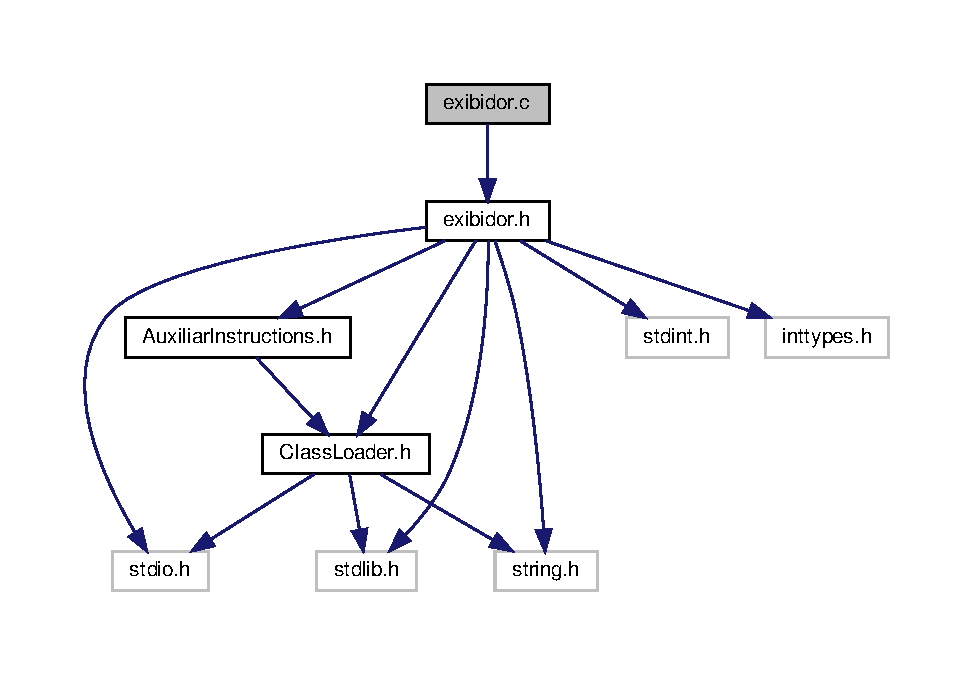
\includegraphics[width=350pt]{exibidor_8c__incl}
\end{center}
\end{figure}

\hypertarget{exibidor_8h}{}\section{Referência do Arquivo exibidor.\+h}
\label{exibidor_8h}\index{exibidor.\+h@{exibidor.\+h}}
{\ttfamily \#include $<$stdio.\+h$>$}\newline
{\ttfamily \#include $<$stdint.\+h$>$}\newline
{\ttfamily \#include $<$inttypes.\+h$>$}\newline
{\ttfamily \#include $<$stdlib.\+h$>$}\newline
{\ttfamily \#include $<$string.\+h$>$}\newline
{\ttfamily \#include \char`\"{}Class\+Loader.\+h\char`\"{}}\newline
{\ttfamily \#include \char`\"{}Auxiliar\+Instructions.\+h\char`\"{}}\newline
Gráfico de dependência de inclusões para exibidor.\+h\+:\nopagebreak
\begin{figure}[H]
\begin{center}
\leavevmode
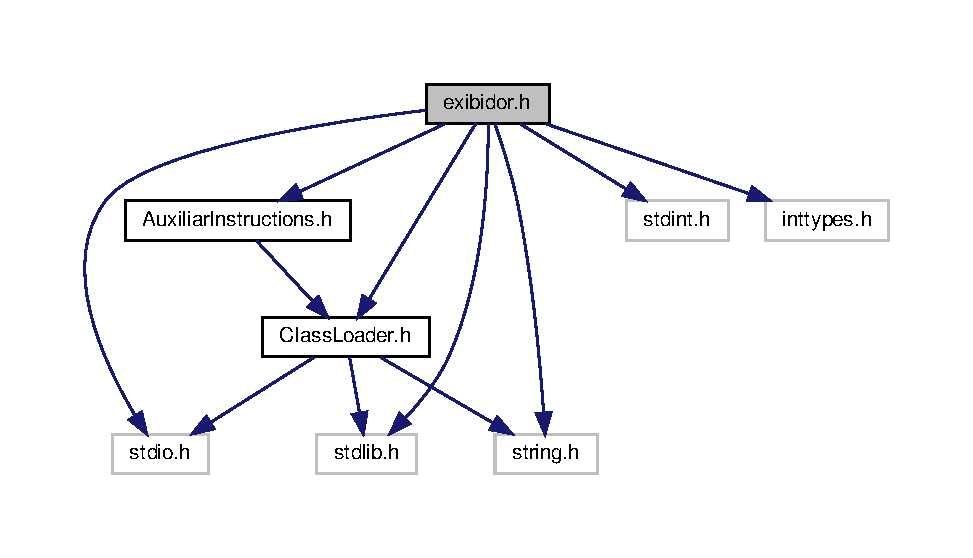
\includegraphics[width=350pt]{exibidor_8h__incl}
\end{center}
\end{figure}
Este grafo mostra quais arquivos estão direta ou indiretamente relacionados com este arquivo\+:\nopagebreak
\begin{figure}[H]
\begin{center}
\leavevmode
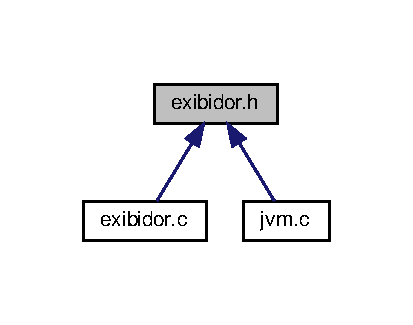
\includegraphics[width=198pt]{exibidor_8h__dep__incl}
\end{center}
\end{figure}
\subsection*{Funções}
\begin{DoxyCompactItemize}
\item 
int \hyperlink{exibidor_8h_a2536a6e3653e6a1d7c3140675d25fdaf}{bit\+\_\+is\+\_\+true} (int code, int id)
\item 
void \hyperlink{exibidor_8h_a1a01812eda71a45ba35d3988240c2cbe}{print\+\_\+flags} (int code, F\+I\+LE $\ast$arq)
\item 
void \hyperlink{exibidor_8h_a4778e7ba3b524b627189f5a12cd2ba58}{print\+\_\+func\+\_\+magic} (\hyperlink{structClassFile}{Class\+File} $\ast$cf, F\+I\+LE $\ast$arq)
\item 
void \hyperlink{exibidor_8h_a48bde3f16c3b4fb1200cfeed966271b3}{print\+\_\+versions} (\hyperlink{structClassFile}{Class\+File} $\ast$cf, F\+I\+LE $\ast$arq)
\item 
void \hyperlink{exibidor_8h_a1afd246a2708493137d6779a8a0949e8}{print\+\_\+constantpool} (\hyperlink{structClassFile}{Class\+File} $\ast$cf, F\+I\+LE $\ast$arq)
\item 
void \hyperlink{exibidor_8h_aa3ee6d33a96bd2d33d1febe2148c89cb}{print\+\_\+classdata} (\hyperlink{structClassFile}{Class\+File} $\ast$cf, F\+I\+LE $\ast$arq)
\item 
void \hyperlink{exibidor_8h_ae816a5183f48e88d2916f7eb3435276f}{print\+\_\+interfaces} (\hyperlink{structClassFile}{Class\+File} $\ast$cf, F\+I\+LE $\ast$arq)
\item 
void \hyperlink{exibidor_8h_a2319a835bb7cb2db0e68a5baee9520d9}{print\+\_\+atribute} (\hyperlink{structClassFile}{Class\+File} $\ast$cf, \hyperlink{structattribute__info}{attribute\+\_\+info} $\ast$att, F\+I\+LE $\ast$arq)
\item 
void \hyperlink{exibidor_8h_a7bf7dfe6bd02790dffee49ca9d2db790}{print\+\_\+fields} (\hyperlink{structClassFile}{Class\+File} $\ast$cf, F\+I\+LE $\ast$arq)
\item 
void \hyperlink{exibidor_8h_a9c6461cf8681e258a54c6ecec7b4af89}{print\+\_\+methodes} (\hyperlink{structClassFile}{Class\+File} $\ast$cf, F\+I\+LE $\ast$arq)
\item 
void \hyperlink{exibidor_8h_abbccca1911c01347bce3a7b3f6ba5880}{print\+\_\+atributes} (\hyperlink{structClassFile}{Class\+File} $\ast$cf, F\+I\+LE $\ast$arq)
\item 
void \hyperlink{exibidor_8h_a847a96c8d54d5a68b6c0161fdd0cbe24}{print\+\_\+class} (\hyperlink{structClassFile}{Class\+File} $\ast$cf, char $\ast$namefile, F\+I\+LE $\ast$arq)
\item 
char $\ast$ \hyperlink{exibidor_8h_a452dd1d3f9dad220fbe70a74adffca67}{look\+\_\+version} (int code)
\end{DoxyCompactItemize}


\subsection{Funções}
\mbox{\Hypertarget{exibidor_8h_a2536a6e3653e6a1d7c3140675d25fdaf}\label{exibidor_8h_a2536a6e3653e6a1d7c3140675d25fdaf}} 
\index{exibidor.\+h@{exibidor.\+h}!bit\+\_\+is\+\_\+true@{bit\+\_\+is\+\_\+true}}
\index{bit\+\_\+is\+\_\+true@{bit\+\_\+is\+\_\+true}!exibidor.\+h@{exibidor.\+h}}
\subsubsection{\texorpdfstring{bit\+\_\+is\+\_\+true()}{bit\_is\_true()}}
{\footnotesize\ttfamily int bit\+\_\+is\+\_\+true (\begin{DoxyParamCaption}\item[{int}]{code,  }\item[{int}]{id }\end{DoxyParamCaption})}

\mbox{\Hypertarget{exibidor_8h_a452dd1d3f9dad220fbe70a74adffca67}\label{exibidor_8h_a452dd1d3f9dad220fbe70a74adffca67}} 
\index{exibidor.\+h@{exibidor.\+h}!look\+\_\+version@{look\+\_\+version}}
\index{look\+\_\+version@{look\+\_\+version}!exibidor.\+h@{exibidor.\+h}}
\subsubsection{\texorpdfstring{look\+\_\+version()}{look\_version()}}
{\footnotesize\ttfamily char$\ast$ look\+\_\+version (\begin{DoxyParamCaption}\item[{int}]{code }\end{DoxyParamCaption})}

\mbox{\Hypertarget{exibidor_8h_a2319a835bb7cb2db0e68a5baee9520d9}\label{exibidor_8h_a2319a835bb7cb2db0e68a5baee9520d9}} 
\index{exibidor.\+h@{exibidor.\+h}!print\+\_\+atribute@{print\+\_\+atribute}}
\index{print\+\_\+atribute@{print\+\_\+atribute}!exibidor.\+h@{exibidor.\+h}}
\subsubsection{\texorpdfstring{print\+\_\+atribute()}{print\_atribute()}}
{\footnotesize\ttfamily void print\+\_\+atribute (\begin{DoxyParamCaption}\item[{\hyperlink{structClassFile}{Class\+File} $\ast$}]{cf,  }\item[{\hyperlink{structattribute__info}{attribute\+\_\+info} $\ast$}]{att,  }\item[{F\+I\+LE $\ast$}]{arq }\end{DoxyParamCaption})}

\mbox{\Hypertarget{exibidor_8h_abbccca1911c01347bce3a7b3f6ba5880}\label{exibidor_8h_abbccca1911c01347bce3a7b3f6ba5880}} 
\index{exibidor.\+h@{exibidor.\+h}!print\+\_\+atributes@{print\+\_\+atributes}}
\index{print\+\_\+atributes@{print\+\_\+atributes}!exibidor.\+h@{exibidor.\+h}}
\subsubsection{\texorpdfstring{print\+\_\+atributes()}{print\_atributes()}}
{\footnotesize\ttfamily void print\+\_\+atributes (\begin{DoxyParamCaption}\item[{\hyperlink{structClassFile}{Class\+File} $\ast$}]{cf,  }\item[{F\+I\+LE $\ast$}]{arq }\end{DoxyParamCaption})}

\mbox{\Hypertarget{exibidor_8h_a847a96c8d54d5a68b6c0161fdd0cbe24}\label{exibidor_8h_a847a96c8d54d5a68b6c0161fdd0cbe24}} 
\index{exibidor.\+h@{exibidor.\+h}!print\+\_\+class@{print\+\_\+class}}
\index{print\+\_\+class@{print\+\_\+class}!exibidor.\+h@{exibidor.\+h}}
\subsubsection{\texorpdfstring{print\+\_\+class()}{print\_class()}}
{\footnotesize\ttfamily void print\+\_\+class (\begin{DoxyParamCaption}\item[{\hyperlink{structClassFile}{Class\+File} $\ast$}]{cf,  }\item[{char $\ast$}]{namefile,  }\item[{F\+I\+LE $\ast$}]{arq }\end{DoxyParamCaption})}

\mbox{\Hypertarget{exibidor_8h_aa3ee6d33a96bd2d33d1febe2148c89cb}\label{exibidor_8h_aa3ee6d33a96bd2d33d1febe2148c89cb}} 
\index{exibidor.\+h@{exibidor.\+h}!print\+\_\+classdata@{print\+\_\+classdata}}
\index{print\+\_\+classdata@{print\+\_\+classdata}!exibidor.\+h@{exibidor.\+h}}
\subsubsection{\texorpdfstring{print\+\_\+classdata()}{print\_classdata()}}
{\footnotesize\ttfamily void print\+\_\+classdata (\begin{DoxyParamCaption}\item[{\hyperlink{structClassFile}{Class\+File} $\ast$}]{cf,  }\item[{F\+I\+LE $\ast$}]{arq }\end{DoxyParamCaption})}

\mbox{\Hypertarget{exibidor_8h_a1afd246a2708493137d6779a8a0949e8}\label{exibidor_8h_a1afd246a2708493137d6779a8a0949e8}} 
\index{exibidor.\+h@{exibidor.\+h}!print\+\_\+constantpool@{print\+\_\+constantpool}}
\index{print\+\_\+constantpool@{print\+\_\+constantpool}!exibidor.\+h@{exibidor.\+h}}
\subsubsection{\texorpdfstring{print\+\_\+constantpool()}{print\_constantpool()}}
{\footnotesize\ttfamily void print\+\_\+constantpool (\begin{DoxyParamCaption}\item[{\hyperlink{structClassFile}{Class\+File} $\ast$}]{cf,  }\item[{F\+I\+LE $\ast$}]{arq }\end{DoxyParamCaption})}

\mbox{\Hypertarget{exibidor_8h_a7bf7dfe6bd02790dffee49ca9d2db790}\label{exibidor_8h_a7bf7dfe6bd02790dffee49ca9d2db790}} 
\index{exibidor.\+h@{exibidor.\+h}!print\+\_\+fields@{print\+\_\+fields}}
\index{print\+\_\+fields@{print\+\_\+fields}!exibidor.\+h@{exibidor.\+h}}
\subsubsection{\texorpdfstring{print\+\_\+fields()}{print\_fields()}}
{\footnotesize\ttfamily void print\+\_\+fields (\begin{DoxyParamCaption}\item[{\hyperlink{structClassFile}{Class\+File} $\ast$}]{cf,  }\item[{F\+I\+LE $\ast$}]{arq }\end{DoxyParamCaption})}

\mbox{\Hypertarget{exibidor_8h_a1a01812eda71a45ba35d3988240c2cbe}\label{exibidor_8h_a1a01812eda71a45ba35d3988240c2cbe}} 
\index{exibidor.\+h@{exibidor.\+h}!print\+\_\+flags@{print\+\_\+flags}}
\index{print\+\_\+flags@{print\+\_\+flags}!exibidor.\+h@{exibidor.\+h}}
\subsubsection{\texorpdfstring{print\+\_\+flags()}{print\_flags()}}
{\footnotesize\ttfamily void print\+\_\+flags (\begin{DoxyParamCaption}\item[{int}]{code,  }\item[{F\+I\+LE $\ast$}]{arq }\end{DoxyParamCaption})}

\mbox{\Hypertarget{exibidor_8h_a4778e7ba3b524b627189f5a12cd2ba58}\label{exibidor_8h_a4778e7ba3b524b627189f5a12cd2ba58}} 
\index{exibidor.\+h@{exibidor.\+h}!print\+\_\+func\+\_\+magic@{print\+\_\+func\+\_\+magic}}
\index{print\+\_\+func\+\_\+magic@{print\+\_\+func\+\_\+magic}!exibidor.\+h@{exibidor.\+h}}
\subsubsection{\texorpdfstring{print\+\_\+func\+\_\+magic()}{print\_func\_magic()}}
{\footnotesize\ttfamily void print\+\_\+func\+\_\+magic (\begin{DoxyParamCaption}\item[{\hyperlink{structClassFile}{Class\+File} $\ast$}]{cf,  }\item[{F\+I\+LE $\ast$}]{arq }\end{DoxyParamCaption})}

\mbox{\Hypertarget{exibidor_8h_ae816a5183f48e88d2916f7eb3435276f}\label{exibidor_8h_ae816a5183f48e88d2916f7eb3435276f}} 
\index{exibidor.\+h@{exibidor.\+h}!print\+\_\+interfaces@{print\+\_\+interfaces}}
\index{print\+\_\+interfaces@{print\+\_\+interfaces}!exibidor.\+h@{exibidor.\+h}}
\subsubsection{\texorpdfstring{print\+\_\+interfaces()}{print\_interfaces()}}
{\footnotesize\ttfamily void print\+\_\+interfaces (\begin{DoxyParamCaption}\item[{\hyperlink{structClassFile}{Class\+File} $\ast$}]{cf,  }\item[{F\+I\+LE $\ast$}]{arq }\end{DoxyParamCaption})}

\mbox{\Hypertarget{exibidor_8h_a9c6461cf8681e258a54c6ecec7b4af89}\label{exibidor_8h_a9c6461cf8681e258a54c6ecec7b4af89}} 
\index{exibidor.\+h@{exibidor.\+h}!print\+\_\+methodes@{print\+\_\+methodes}}
\index{print\+\_\+methodes@{print\+\_\+methodes}!exibidor.\+h@{exibidor.\+h}}
\subsubsection{\texorpdfstring{print\+\_\+methodes()}{print\_methodes()}}
{\footnotesize\ttfamily void print\+\_\+methodes (\begin{DoxyParamCaption}\item[{\hyperlink{structClassFile}{Class\+File} $\ast$}]{cf,  }\item[{F\+I\+LE $\ast$}]{arq }\end{DoxyParamCaption})}

\mbox{\Hypertarget{exibidor_8h_a48bde3f16c3b4fb1200cfeed966271b3}\label{exibidor_8h_a48bde3f16c3b4fb1200cfeed966271b3}} 
\index{exibidor.\+h@{exibidor.\+h}!print\+\_\+versions@{print\+\_\+versions}}
\index{print\+\_\+versions@{print\+\_\+versions}!exibidor.\+h@{exibidor.\+h}}
\subsubsection{\texorpdfstring{print\+\_\+versions()}{print\_versions()}}
{\footnotesize\ttfamily void print\+\_\+versions (\begin{DoxyParamCaption}\item[{\hyperlink{structClassFile}{Class\+File} $\ast$}]{cf,  }\item[{F\+I\+LE $\ast$}]{arq }\end{DoxyParamCaption})}


\hypertarget{FrameStack_8c}{}\section{Referência do Arquivo Frame\+Stack.\+c}
\label{FrameStack_8c}\index{Frame\+Stack.\+c@{Frame\+Stack.\+c}}
{\ttfamily \#include $<$stdlib.\+h$>$}\newline
{\ttfamily \#include \char`\"{}Frame\+Stack.\+h\char`\"{}}\newline
Gráfico de dependência de inclusões para Frame\+Stack.\+c\+:\nopagebreak
\begin{figure}[H]
\begin{center}
\leavevmode
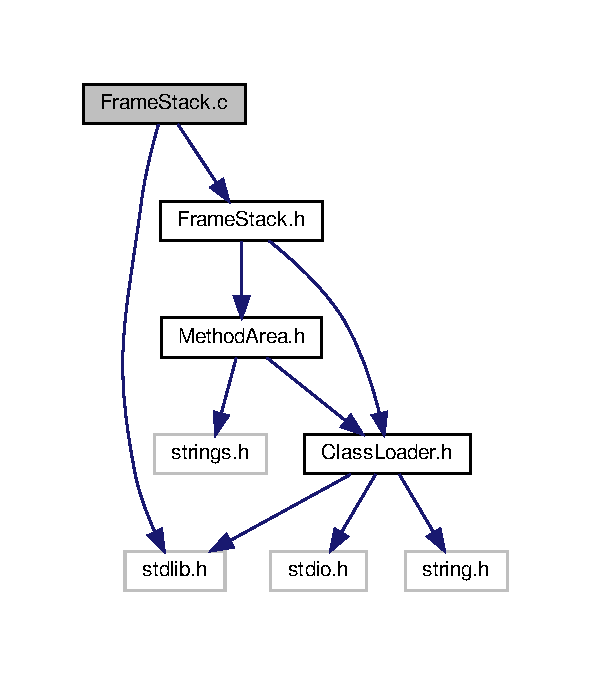
\includegraphics[width=284pt]{FrameStack_8c__incl}
\end{center}
\end{figure}
\subsection*{Funções}
\begin{DoxyCompactItemize}
\item 
void \hyperlink{FrameStack_8c_a605a09336c06cbc72668767f80bc0865}{push\+\_\+frame} (\hyperlink{structcp__info}{cp\+\_\+info} $\ast$cp, \hyperlink{structStaticAtrib}{Static\+Atrib} $\ast$sa, \hyperlink{structmethod__info}{method\+\_\+info} $\ast$mf, \hyperlink{structFrameStack}{Frame\+Stack} $\ast$fs)
\begin{DoxyCompactList}\small\item\em Função que adiciona um frame. \end{DoxyCompactList}\item 
void \hyperlink{FrameStack_8c_a0023f807f16e23c4bf72546e035d6c7d}{pop\+\_\+frame} (\hyperlink{structFrameStack}{Frame\+Stack} $\ast$fs)
\item 
void \hyperlink{FrameStack_8c_a58e0fe52e8e68e2d658615da24266b9b}{push\+\_\+operand} (\hyperlink{ClassLoader_8h_aedf6ddc03df8caaaccbb4c60b9a9b850}{u4} data, \hyperlink{structoperand__stack}{operand\+\_\+stack} $\ast$opstack)
\begin{DoxyCompactList}\small\item\em Função que coloca um operando na pilha. \end{DoxyCompactList}\item 
void \hyperlink{FrameStack_8c_aa1cfd3f59256a45cef0b2308c57d1b1a}{free\+\_\+operand\+\_\+stack} (\hyperlink{structoperand__stack}{operand\+\_\+stack} $\ast$opstack)
\begin{DoxyCompactList}\small\item\em Função que libera a pilha da memória. \end{DoxyCompactList}\item 
\hyperlink{ClassLoader_8h_aedf6ddc03df8caaaccbb4c60b9a9b850}{u4} \hyperlink{FrameStack_8c_a5316e1c063f566340878c6e5564c11a7}{pop\+\_\+operand} (\hyperlink{structoperand__stack}{operand\+\_\+stack} $\ast$opstack)
\begin{DoxyCompactList}\small\item\em Função que desempilha um operando da pilha. \end{DoxyCompactList}\end{DoxyCompactItemize}


\subsection{Funções}
\mbox{\Hypertarget{FrameStack_8c_aa1cfd3f59256a45cef0b2308c57d1b1a}\label{FrameStack_8c_aa1cfd3f59256a45cef0b2308c57d1b1a}} 
\index{Frame\+Stack.\+c@{Frame\+Stack.\+c}!free\+\_\+operand\+\_\+stack@{free\+\_\+operand\+\_\+stack}}
\index{free\+\_\+operand\+\_\+stack@{free\+\_\+operand\+\_\+stack}!Frame\+Stack.\+c@{Frame\+Stack.\+c}}
\subsubsection{\texorpdfstring{free\+\_\+operand\+\_\+stack()}{free\_operand\_stack()}}
{\footnotesize\ttfamily void free\+\_\+operand\+\_\+stack (\begin{DoxyParamCaption}\item[{\hyperlink{structoperand__stack}{operand\+\_\+stack} $\ast$}]{opstack }\end{DoxyParamCaption})}



Função que libera a pilha da memória. 


\begin{DoxyParams}{Parâmetros}
{\em $\ast$opstack} & ponteiro para a pilha \\
\hline
\end{DoxyParams}
\mbox{\Hypertarget{FrameStack_8c_a0023f807f16e23c4bf72546e035d6c7d}\label{FrameStack_8c_a0023f807f16e23c4bf72546e035d6c7d}} 
\index{Frame\+Stack.\+c@{Frame\+Stack.\+c}!pop\+\_\+frame@{pop\+\_\+frame}}
\index{pop\+\_\+frame@{pop\+\_\+frame}!Frame\+Stack.\+c@{Frame\+Stack.\+c}}
\subsubsection{\texorpdfstring{pop\+\_\+frame()}{pop\_frame()}}
{\footnotesize\ttfamily void pop\+\_\+frame (\begin{DoxyParamCaption}\item[{\hyperlink{structFrameStack}{Frame\+Stack} $\ast$}]{fs }\end{DoxyParamCaption})}

\mbox{\Hypertarget{FrameStack_8c_a5316e1c063f566340878c6e5564c11a7}\label{FrameStack_8c_a5316e1c063f566340878c6e5564c11a7}} 
\index{Frame\+Stack.\+c@{Frame\+Stack.\+c}!pop\+\_\+operand@{pop\+\_\+operand}}
\index{pop\+\_\+operand@{pop\+\_\+operand}!Frame\+Stack.\+c@{Frame\+Stack.\+c}}
\subsubsection{\texorpdfstring{pop\+\_\+operand()}{pop\_operand()}}
{\footnotesize\ttfamily \hyperlink{ClassLoader_8h_aedf6ddc03df8caaaccbb4c60b9a9b850}{u4} pop\+\_\+operand (\begin{DoxyParamCaption}\item[{\hyperlink{structoperand__stack}{operand\+\_\+stack} $\ast$}]{stack }\end{DoxyParamCaption})}



Função que desempilha um operando da pilha. 


\begin{DoxyParams}{Parâmetros}
{\em $\ast$stack} & ponteiro para a pilha \\
\hline
\end{DoxyParams}
\begin{DoxyReturn}{Retorna}
O operando desimpilhado 
\end{DoxyReturn}
\mbox{\Hypertarget{FrameStack_8c_a605a09336c06cbc72668767f80bc0865}\label{FrameStack_8c_a605a09336c06cbc72668767f80bc0865}} 
\index{Frame\+Stack.\+c@{Frame\+Stack.\+c}!push\+\_\+frame@{push\+\_\+frame}}
\index{push\+\_\+frame@{push\+\_\+frame}!Frame\+Stack.\+c@{Frame\+Stack.\+c}}
\subsubsection{\texorpdfstring{push\+\_\+frame()}{push\_frame()}}
{\footnotesize\ttfamily void push\+\_\+frame (\begin{DoxyParamCaption}\item[{\hyperlink{structcp__info}{cp\+\_\+info} $\ast$}]{cp,  }\item[{\hyperlink{structStaticAtrib}{Static\+Atrib} $\ast$}]{sa,  }\item[{\hyperlink{structmethod__info}{method\+\_\+info} $\ast$}]{mf,  }\item[{\hyperlink{structFrameStack}{Frame\+Stack} $\ast$}]{fs }\end{DoxyParamCaption})}



Função que adiciona um frame. 


\begin{DoxyParams}{Parâmetros}
{\em $\ast$cp} & Ponteiro para o constant pool \\
\hline
{\em $\ast$mf} & Ponteiro para as informações do método \\
\hline
{\em $\ast$fs} & Ponteiro para a pilha de frames \\
\hline
\end{DoxyParams}
\mbox{\Hypertarget{FrameStack_8c_a58e0fe52e8e68e2d658615da24266b9b}\label{FrameStack_8c_a58e0fe52e8e68e2d658615da24266b9b}} 
\index{Frame\+Stack.\+c@{Frame\+Stack.\+c}!push\+\_\+operand@{push\+\_\+operand}}
\index{push\+\_\+operand@{push\+\_\+operand}!Frame\+Stack.\+c@{Frame\+Stack.\+c}}
\subsubsection{\texorpdfstring{push\+\_\+operand()}{push\_operand()}}
{\footnotesize\ttfamily void push\+\_\+operand (\begin{DoxyParamCaption}\item[{\hyperlink{ClassLoader_8h_aedf6ddc03df8caaaccbb4c60b9a9b850}{u4}}]{data,  }\item[{\hyperlink{structoperand__stack}{operand\+\_\+stack} $\ast$}]{stack }\end{DoxyParamCaption})}



Função que coloca um operando na pilha. 


\begin{DoxyParams}{Parâmetros}
{\em data} & O operando a ser empilhado \\
\hline
{\em $\ast$stack} & ponteiro para a pilha \\
\hline
\end{DoxyParams}

\hypertarget{FrameStack_8h}{}\section{Referência do Arquivo Frame\+Stack.\+h}
\label{FrameStack_8h}\index{Frame\+Stack.\+h@{Frame\+Stack.\+h}}
{\ttfamily \#include \char`\"{}Method\+Area.\+h\char`\"{}}\newline
{\ttfamily \#include \char`\"{}Class\+Loader.\+h\char`\"{}}\newline
Gráfico de dependência de inclusões para Frame\+Stack.\+h\+:\nopagebreak
\begin{figure}[H]
\begin{center}
\leavevmode
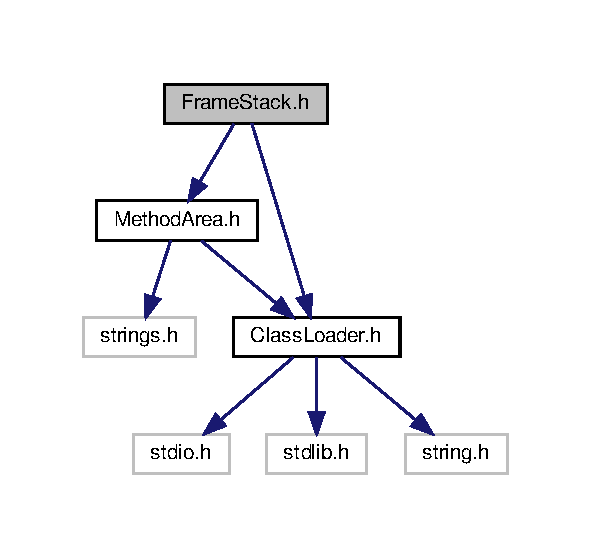
\includegraphics[width=284pt]{FrameStack_8h__incl}
\end{center}
\end{figure}
Este grafo mostra quais arquivos estão direta ou indiretamente relacionados com este arquivo\+:\nopagebreak
\begin{figure}[H]
\begin{center}
\leavevmode
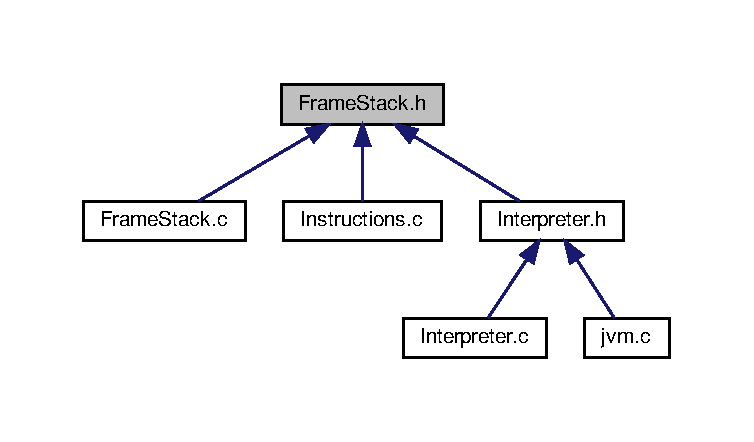
\includegraphics[width=350pt]{FrameStack_8h__dep__incl}
\end{center}
\end{figure}
\subsection*{Componentes}
\begin{DoxyCompactItemize}
\item 
struct \hyperlink{structoperand}{operand}
\item 
struct \hyperlink{structoperand__stack}{operand\+\_\+stack}
\begin{DoxyCompactList}\small\item\em Estrutura da pilha propriamente dita. \end{DoxyCompactList}\item 
struct \hyperlink{structframe}{frame}
\begin{DoxyCompactList}\small\item\em Estrutura dos elementos da pilha de frames. \end{DoxyCompactList}\item 
struct \hyperlink{structFrameStack}{Frame\+Stack}
\begin{DoxyCompactList}\small\item\em Estrutura da pilha de frames. \end{DoxyCompactList}\end{DoxyCompactItemize}
\subsection*{Definições de Tipos}
\begin{DoxyCompactItemize}
\item 
typedef struct \hyperlink{structoperand}{operand} \hyperlink{FrameStack_8h_a35236647a2ad82ec456f438503e59d11}{stack}
\item 
typedef struct \hyperlink{structoperand__stack}{operand\+\_\+stack} \hyperlink{FrameStack_8h_a2ede843ae23dfbb88d1e68890580b97a}{operand\+\_\+stack}
\begin{DoxyCompactList}\small\item\em Estrutura da pilha propriamente dita. \end{DoxyCompactList}\item 
typedef struct \hyperlink{structframe}{frame} \hyperlink{FrameStack_8h_aa02f79e5cf231f7fcd7bdf8e647fe96e}{frame}
\begin{DoxyCompactList}\small\item\em Estrutura dos elementos da pilha de frames. \end{DoxyCompactList}\item 
typedef struct \hyperlink{structFrameStack}{Frame\+Stack} \hyperlink{FrameStack_8h_ab4bdf0a3d1b174c241124cb6b89dcaef}{Frame\+Stack}
\begin{DoxyCompactList}\small\item\em Estrutura da pilha de frames. \end{DoxyCompactList}\end{DoxyCompactItemize}
\subsection*{Funções}
\begin{DoxyCompactItemize}
\item 
void \hyperlink{FrameStack_8h_adf405e4f609a9f435b67ef5aae21bb29}{push\+\_\+operand} (\hyperlink{ClassLoader_8h_aedf6ddc03df8caaaccbb4c60b9a9b850}{u4} data, \hyperlink{structoperand__stack}{operand\+\_\+stack} $\ast$\hyperlink{FrameStack_8h_a35236647a2ad82ec456f438503e59d11}{stack})
\begin{DoxyCompactList}\small\item\em Função que coloca um operando na pilha. \end{DoxyCompactList}\item 
\hyperlink{ClassLoader_8h_aedf6ddc03df8caaaccbb4c60b9a9b850}{u4} \hyperlink{FrameStack_8h_a399acbcb53bc89fa98f48faf5af41ba2}{pop\+\_\+operand} (\hyperlink{structoperand__stack}{operand\+\_\+stack} $\ast$\hyperlink{FrameStack_8h_a35236647a2ad82ec456f438503e59d11}{stack})
\begin{DoxyCompactList}\small\item\em Função que desempilha um operando da pilha. \end{DoxyCompactList}\item 
void \hyperlink{FrameStack_8h_aa1cfd3f59256a45cef0b2308c57d1b1a}{free\+\_\+operand\+\_\+stack} (\hyperlink{structoperand__stack}{operand\+\_\+stack} $\ast$opstack)
\begin{DoxyCompactList}\small\item\em Função que libera a pilha da memória. \end{DoxyCompactList}\item 
void \hyperlink{FrameStack_8h_a605a09336c06cbc72668767f80bc0865}{push\+\_\+frame} (\hyperlink{structcp__info}{cp\+\_\+info} $\ast$cp, \hyperlink{structStaticAtrib}{Static\+Atrib} $\ast$sa, \hyperlink{structmethod__info}{method\+\_\+info} $\ast$mf, \hyperlink{structFrameStack}{Frame\+Stack} $\ast$fs)
\begin{DoxyCompactList}\small\item\em Função que adiciona um frame. \end{DoxyCompactList}\item 
void \hyperlink{FrameStack_8h_a73dce0d70d5626fd174e379d1affbd1f}{pop\+\_\+frame} (\hyperlink{structFrameStack}{Frame\+Stack} $\ast$sf)
\end{DoxyCompactItemize}


\subsection{Definições dos tipos}
\mbox{\Hypertarget{FrameStack_8h_aa02f79e5cf231f7fcd7bdf8e647fe96e}\label{FrameStack_8h_aa02f79e5cf231f7fcd7bdf8e647fe96e}} 
\index{Frame\+Stack.\+h@{Frame\+Stack.\+h}!frame@{frame}}
\index{frame@{frame}!Frame\+Stack.\+h@{Frame\+Stack.\+h}}
\subsubsection{\texorpdfstring{frame}{frame}}
{\footnotesize\ttfamily typedef struct \hyperlink{structframe}{frame} \hyperlink{structframe}{frame}}



Estrutura dos elementos da pilha de frames. 

\mbox{\Hypertarget{FrameStack_8h_ab4bdf0a3d1b174c241124cb6b89dcaef}\label{FrameStack_8h_ab4bdf0a3d1b174c241124cb6b89dcaef}} 
\index{Frame\+Stack.\+h@{Frame\+Stack.\+h}!Frame\+Stack@{Frame\+Stack}}
\index{Frame\+Stack@{Frame\+Stack}!Frame\+Stack.\+h@{Frame\+Stack.\+h}}
\subsubsection{\texorpdfstring{Frame\+Stack}{FrameStack}}
{\footnotesize\ttfamily typedef struct \hyperlink{structFrameStack}{Frame\+Stack} \hyperlink{structFrameStack}{Frame\+Stack}}



Estrutura da pilha de frames. 

\mbox{\Hypertarget{FrameStack_8h_a2ede843ae23dfbb88d1e68890580b97a}\label{FrameStack_8h_a2ede843ae23dfbb88d1e68890580b97a}} 
\index{Frame\+Stack.\+h@{Frame\+Stack.\+h}!operand\+\_\+stack@{operand\+\_\+stack}}
\index{operand\+\_\+stack@{operand\+\_\+stack}!Frame\+Stack.\+h@{Frame\+Stack.\+h}}
\subsubsection{\texorpdfstring{operand\+\_\+stack}{operand\_stack}}
{\footnotesize\ttfamily typedef struct \hyperlink{structoperand__stack}{operand\+\_\+stack} \hyperlink{structoperand__stack}{operand\+\_\+stack}}



Estrutura da pilha propriamente dita. 

\mbox{\Hypertarget{FrameStack_8h_a35236647a2ad82ec456f438503e59d11}\label{FrameStack_8h_a35236647a2ad82ec456f438503e59d11}} 
\index{Frame\+Stack.\+h@{Frame\+Stack.\+h}!stack@{stack}}
\index{stack@{stack}!Frame\+Stack.\+h@{Frame\+Stack.\+h}}
\subsubsection{\texorpdfstring{stack}{stack}}
{\footnotesize\ttfamily typedef struct \hyperlink{structoperand}{operand} \hyperlink{FrameStack_8h_a35236647a2ad82ec456f438503e59d11}{stack}}



\subsection{Funções}
\mbox{\Hypertarget{FrameStack_8h_aa1cfd3f59256a45cef0b2308c57d1b1a}\label{FrameStack_8h_aa1cfd3f59256a45cef0b2308c57d1b1a}} 
\index{Frame\+Stack.\+h@{Frame\+Stack.\+h}!free\+\_\+operand\+\_\+stack@{free\+\_\+operand\+\_\+stack}}
\index{free\+\_\+operand\+\_\+stack@{free\+\_\+operand\+\_\+stack}!Frame\+Stack.\+h@{Frame\+Stack.\+h}}
\subsubsection{\texorpdfstring{free\+\_\+operand\+\_\+stack()}{free\_operand\_stack()}}
{\footnotesize\ttfamily void free\+\_\+operand\+\_\+stack (\begin{DoxyParamCaption}\item[{\hyperlink{structoperand__stack}{operand\+\_\+stack} $\ast$}]{opstack }\end{DoxyParamCaption})}



Função que libera a pilha da memória. 


\begin{DoxyParams}{Parâmetros}
{\em $\ast$opstack} & ponteiro para a pilha \\
\hline
\end{DoxyParams}
\mbox{\Hypertarget{FrameStack_8h_a73dce0d70d5626fd174e379d1affbd1f}\label{FrameStack_8h_a73dce0d70d5626fd174e379d1affbd1f}} 
\index{Frame\+Stack.\+h@{Frame\+Stack.\+h}!pop\+\_\+frame@{pop\+\_\+frame}}
\index{pop\+\_\+frame@{pop\+\_\+frame}!Frame\+Stack.\+h@{Frame\+Stack.\+h}}
\subsubsection{\texorpdfstring{pop\+\_\+frame()}{pop\_frame()}}
{\footnotesize\ttfamily void pop\+\_\+frame (\begin{DoxyParamCaption}\item[{\hyperlink{structFrameStack}{Frame\+Stack} $\ast$}]{sf }\end{DoxyParamCaption})}

\mbox{\Hypertarget{FrameStack_8h_a399acbcb53bc89fa98f48faf5af41ba2}\label{FrameStack_8h_a399acbcb53bc89fa98f48faf5af41ba2}} 
\index{Frame\+Stack.\+h@{Frame\+Stack.\+h}!pop\+\_\+operand@{pop\+\_\+operand}}
\index{pop\+\_\+operand@{pop\+\_\+operand}!Frame\+Stack.\+h@{Frame\+Stack.\+h}}
\subsubsection{\texorpdfstring{pop\+\_\+operand()}{pop\_operand()}}
{\footnotesize\ttfamily \hyperlink{ClassLoader_8h_aedf6ddc03df8caaaccbb4c60b9a9b850}{u4} pop\+\_\+operand (\begin{DoxyParamCaption}\item[{\hyperlink{structoperand__stack}{operand\+\_\+stack} $\ast$}]{stack }\end{DoxyParamCaption})}



Função que desempilha um operando da pilha. 


\begin{DoxyParams}{Parâmetros}
{\em $\ast$stack} & ponteiro para a pilha \\
\hline
\end{DoxyParams}
\begin{DoxyReturn}{Retorna}
O operando desimpilhado 
\end{DoxyReturn}
\mbox{\Hypertarget{FrameStack_8h_a605a09336c06cbc72668767f80bc0865}\label{FrameStack_8h_a605a09336c06cbc72668767f80bc0865}} 
\index{Frame\+Stack.\+h@{Frame\+Stack.\+h}!push\+\_\+frame@{push\+\_\+frame}}
\index{push\+\_\+frame@{push\+\_\+frame}!Frame\+Stack.\+h@{Frame\+Stack.\+h}}
\subsubsection{\texorpdfstring{push\+\_\+frame()}{push\_frame()}}
{\footnotesize\ttfamily void push\+\_\+frame (\begin{DoxyParamCaption}\item[{\hyperlink{structcp__info}{cp\+\_\+info} $\ast$}]{cp,  }\item[{\hyperlink{structStaticAtrib}{Static\+Atrib} $\ast$}]{sa,  }\item[{\hyperlink{structmethod__info}{method\+\_\+info} $\ast$}]{mf,  }\item[{\hyperlink{structFrameStack}{Frame\+Stack} $\ast$}]{fs }\end{DoxyParamCaption})}



Função que adiciona um frame. 


\begin{DoxyParams}{Parâmetros}
{\em $\ast$cp} & Ponteiro para o constant pool \\
\hline
{\em $\ast$mf} & Ponteiro para as informações do método \\
\hline
{\em $\ast$fs} & Ponteiro para a pilha de frames \\
\hline
\end{DoxyParams}
\mbox{\Hypertarget{FrameStack_8h_adf405e4f609a9f435b67ef5aae21bb29}\label{FrameStack_8h_adf405e4f609a9f435b67ef5aae21bb29}} 
\index{Frame\+Stack.\+h@{Frame\+Stack.\+h}!push\+\_\+operand@{push\+\_\+operand}}
\index{push\+\_\+operand@{push\+\_\+operand}!Frame\+Stack.\+h@{Frame\+Stack.\+h}}
\subsubsection{\texorpdfstring{push\+\_\+operand()}{push\_operand()}}
{\footnotesize\ttfamily void push\+\_\+operand (\begin{DoxyParamCaption}\item[{\hyperlink{ClassLoader_8h_aedf6ddc03df8caaaccbb4c60b9a9b850}{u4}}]{data,  }\item[{\hyperlink{structoperand__stack}{operand\+\_\+stack} $\ast$}]{stack }\end{DoxyParamCaption})}



Função que coloca um operando na pilha. 


\begin{DoxyParams}{Parâmetros}
{\em data} & O operando a ser empilhado \\
\hline
{\em $\ast$stack} & ponteiro para a pilha \\
\hline
\end{DoxyParams}

\hypertarget{Instructions_8c}{}\section{Referência do Arquivo Instructions.\+c}
\label{Instructions_8c}\index{Instructions.\+c@{Instructions.\+c}}
{\ttfamily \#include $<$stdio.\+h$>$}\newline
{\ttfamily \#include \char`\"{}Frame\+Stack.\+h\char`\"{}}\newline
{\ttfamily \#include \char`\"{}Instructions.\+h\char`\"{}}\newline
Gráfico de dependência de inclusões para Instructions.\+c\+:
\nopagebreak
\begin{figure}[H]
\begin{center}
\leavevmode
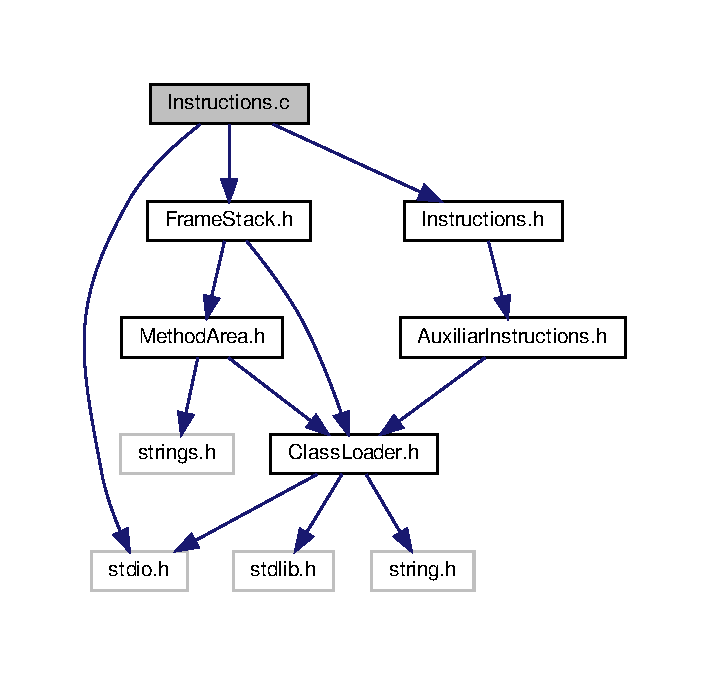
\includegraphics[width=340pt]{Instructions_8c__incl}
\end{center}
\end{figure}
\subsection*{Funções}
\begin{DoxyCompactItemize}
\item 
void \hyperlink{Instructions_8c_a705dd2fba1996967769549452c8266e1}{bipush} (char valor, \hyperlink{structFrameStack}{Frame\+Stack} $\ast$fs)
\begin{DoxyCompactList}\small\item\em Esta fun��o empilha um imediato de um byte. \end{DoxyCompactList}\item 
void \hyperlink{Instructions_8c_ad0af00102fb7621045a1c6035acfe5eb}{getstatic} (\hyperlink{structFrameStack}{Frame\+Stack} $\ast$fs)
\begin{DoxyCompactList}\small\item\em Esta fun��o coloca no frame o operador est�tico. \end{DoxyCompactList}\item 
void \hyperlink{Instructions_8c_ac3b98fd98a5a66d5a193e31249f87ab5}{putstatic} (\hyperlink{structFrameStack}{Frame\+Stack} $\ast$fs)
\begin{DoxyCompactList}\small\item\em Esta fun��o desempilha o valor est�tico de um atributo de uma classe, e faz uma atribui��o ao campo. \end{DoxyCompactList}\item 
void \hyperlink{Instructions_8c_a532851306e97050026eb46435c61e9cd}{ldc} (\hyperlink{structFrameStack}{Frame\+Stack} $\ast$fs)
\begin{DoxyCompactList}\small\item\em Esta fun��o busca uma constante no pool de constantes e a empilha na pilha de operandos. \end{DoxyCompactList}\item 
void \hyperlink{Instructions_8c_af89834744bb8c53ff1223c62af02df94}{ldc2} (\hyperlink{structFrameStack}{Frame\+Stack} $\ast$fs)
\begin{DoxyCompactList}\small\item\em Esta fun��o busca uma constante no pool de constantes e a empilha na pilha de operandos. \end{DoxyCompactList}\item 
void \hyperlink{Instructions_8c_a9774fa7ccf4436f3bd486ecba45f7b72}{iconst} (\hyperlink{ClassLoader_8h_aedf6ddc03df8caaaccbb4c60b9a9b850}{u4} val, \hyperlink{structFrameStack}{Frame\+Stack} $\ast$fs)
\begin{DoxyCompactList}\small\item\em Esta função empilha um valor constante na pilha de operandos. \end{DoxyCompactList}\item 
void \hyperlink{Instructions_8c_a14ee4849c176450df2d8c109872abf7f}{istoren} (\hyperlink{ClassLoader_8h_aedf6ddc03df8caaaccbb4c60b9a9b850}{u4} val, \hyperlink{structFrameStack}{Frame\+Stack} $\ast$fs)
\begin{DoxyCompactList}\small\item\em Esta função simplesmente armazena um int do topo da pilha de operandos no vetor de variáveis locais. \end{DoxyCompactList}\item 
void \hyperlink{Instructions_8c_a49c874473ab4ef46868606485ee972c6}{iloadn} (\hyperlink{ClassLoader_8h_aedf6ddc03df8caaaccbb4c60b9a9b850}{u4} val, \hyperlink{structFrameStack}{Frame\+Stack} $\ast$fs)
\begin{DoxyCompactList}\small\item\em Esta função simplesmente carrega um int na pilha de operandos. \end{DoxyCompactList}\item 
void \hyperlink{Instructions_8c_a45ea65a52b6ea9e735727875934b8c47}{iload} (\hyperlink{structFrameStack}{Frame\+Stack} $\ast$fs)
\begin{DoxyCompactList}\small\item\em Esta função simplesmente carrega um int na pilha de operandos. \end{DoxyCompactList}\item 
void \hyperlink{Instructions_8c_a8c01e95c269879a1dc1a93334274b3a4}{istore} (\hyperlink{structFrameStack}{Frame\+Stack} $\ast$fs)
\begin{DoxyCompactList}\small\item\em Esta fun��o simplesmente armazena um int do topo da pilha de operandos no vetor de vari�veis locais. \end{DoxyCompactList}\item 
void \hyperlink{Instructions_8c_add0fcbb1828f4213f1604c9d6305e9f0}{imul} (\hyperlink{structFrameStack}{Frame\+Stack} $\ast$fs)
\begin{DoxyCompactList}\small\item\em Esta função multiplica dois valores inteiros. \end{DoxyCompactList}\item 
void \hyperlink{Instructions_8c_a623503ebec3f0a1528a72dc4299d79db}{iadd} (\hyperlink{structFrameStack}{Frame\+Stack} $\ast$fs)
\begin{DoxyCompactList}\small\item\em Esta função soma dois valores inteiros. \end{DoxyCompactList}\item 
void \hyperlink{Instructions_8c_a9f7af649faabeddfda007b01ce895ba3}{isub} (\hyperlink{structFrameStack}{Frame\+Stack} $\ast$fs)
\begin{DoxyCompactList}\small\item\em Esta função subtrai dois valores inteiros. \end{DoxyCompactList}\item 
void \hyperlink{Instructions_8c_a4f9e7c6193392fe8824266697f51fcf5}{idiv} (\hyperlink{structFrameStack}{Frame\+Stack} $\ast$fs)
\begin{DoxyCompactList}\small\item\em Esta função divide dois valores inteiros. \end{DoxyCompactList}\item 
void \hyperlink{Instructions_8c_acfc35c6f495590de03ec16bb410fa2eb}{iand} (\hyperlink{structFrameStack}{Frame\+Stack} $\ast$fs)
\begin{DoxyCompactList}\small\item\em Esta função faz a operação \char`\"{}e\char`\"{} logico entre dois valores inteiros. \end{DoxyCompactList}\item 
void \hyperlink{Instructions_8c_a0a547b62f2d2962310ea9d0f77666a89}{ineg} (\hyperlink{structFrameStack}{Frame\+Stack} $\ast$fs)
\begin{DoxyCompactList}\small\item\em Esta função passa o valor para negativo de um inteiro. \end{DoxyCompactList}\item 
void \hyperlink{Instructions_8c_a90f4258b5f87aa1547bb969718ebd90e}{ior} (\hyperlink{structFrameStack}{Frame\+Stack} $\ast$fs)
\begin{DoxyCompactList}\small\item\em Esta função faz a operação \char`\"{}ou\char`\"{} logico entre dois valores inteiros. \end{DoxyCompactList}\item 
void \hyperlink{Instructions_8c_a6f1742a279efdafe9a8e35e0cfe70bc5}{ixor} (\hyperlink{structFrameStack}{Frame\+Stack} $\ast$fs)
\begin{DoxyCompactList}\small\item\em Esta função faz a operação logica \char`\"{}xor\char`\"{} entre dois valores inteiros. \end{DoxyCompactList}\item 
void \hyperlink{Instructions_8c_a5431f64e760037b20933b1ec0ff8c932}{irem} (\hyperlink{structFrameStack}{Frame\+Stack} $\ast$fs)
\begin{DoxyCompactList}\small\item\em Esta função pela o resto de uma divisão inteira. \end{DoxyCompactList}\item 
void \hyperlink{Instructions_8c_a5a47a84af9ce9210583e2b34e7e8ca17}{ishl} (\hyperlink{structFrameStack}{Frame\+Stack} $\ast$fs)
\begin{DoxyCompactList}\small\item\em Esta função faz o deslocamento de bits a esquerda de valores inteiros. \end{DoxyCompactList}\item 
void \hyperlink{Instructions_8c_ad7436a2936e0f5648f5e4341c51ebdcf}{ishr} (\hyperlink{structFrameStack}{Frame\+Stack} $\ast$fs)
\begin{DoxyCompactList}\small\item\em Esta função faz o deslocamento de bits a direita de valores inteiros. \end{DoxyCompactList}\item 
void \hyperlink{Instructions_8c_adf61ef75f4895aa3a4db1e3144a85816}{iushr} (\hyperlink{structFrameStack}{Frame\+Stack} $\ast$fs)
\begin{DoxyCompactList}\small\item\em Esta função faz o deslocamento de bits a direita de valores inteiros. \end{DoxyCompactList}\item 
void \hyperlink{Instructions_8c_a4f64f89ab6d89fec030df9acc88b730d}{i2f} (\hyperlink{structFrameStack}{Frame\+Stack} $\ast$fs)
\begin{DoxyCompactList}\small\item\em Esta função coverte um valor inteiro para o tipo float. \end{DoxyCompactList}\item 
void \hyperlink{Instructions_8c_af705acf601f1223a0f9f7e839d6a16ed}{ireturn} (\hyperlink{structFrameStack}{Frame\+Stack} $\ast$fs)
\begin{DoxyCompactList}\small\item\em Esta funçao executa o retorno de um metodo, empilhando o valor int de retorno na pilha de operandos do frame do metodo chamador. \end{DoxyCompactList}\item 
void \hyperlink{Instructions_8c_a984ee14a3d1305398a30d71a39a31e2b}{if\+\_\+icmpge} (\hyperlink{structFrameStack}{Frame\+Stack} $\ast$fs)
\begin{DoxyCompactList}\small\item\em Esta fun��o retira dois elementos do topo da pilha, e calcula um offset a partir do qual PC deve ser incrementado para alcan�ar a pr�xima instru��o. \end{DoxyCompactList}\item 
void \hyperlink{Instructions_8c_a781631e63f47b9950053aca869f6beda}{if\+\_\+icmplt} (\hyperlink{structFrameStack}{Frame\+Stack} $\ast$fs)
\begin{DoxyCompactList}\small\item\em Esta fun��o compara se o valor no topo da pilha de operandos � maior que o segundo valor, e calcula o offset a partir do qual PC deve ser incrementado para alcan�ar a pr�xima instru��o. \end{DoxyCompactList}\item 
void \hyperlink{Instructions_8c_ab97d9bee28ad74380ccf16fdb0891dec}{if\+\_\+icmpeq} (\hyperlink{structFrameStack}{Frame\+Stack} $\ast$fs)
\begin{DoxyCompactList}\small\item\em Esta fun��o compara os dois valores inteiros no topo da pilha de operandos, e calcula o offset a partir do qual PC deve ser incrementado para alcan�ar a pr�xima instru��o. \end{DoxyCompactList}\item 
void \hyperlink{Instructions_8c_a98218ae00da49f5e14d869765a1d430b}{if\+\_\+icmpne} (\hyperlink{structFrameStack}{Frame\+Stack} $\ast$fs)
\begin{DoxyCompactList}\small\item\em Esta fun��o compara os dois valores inteiros no topo da pilha de operandos, e calcula o offset a partir do qual PC deve ser incrementado para alcan�ar a pr�xima instru��o. \end{DoxyCompactList}\item 
void \hyperlink{Instructions_8c_aaf08c7dcf4830be0ca8c009322d7afa8}{if\+\_\+icmpgt} (\hyperlink{structFrameStack}{Frame\+Stack} $\ast$fs)
\begin{DoxyCompactList}\small\item\em Esta fun��o retira dois elementos do topo da pilha, e produz um offset a partir do qual PC deve ser incrementado para alcan�ar a pr�xima instru��o. \end{DoxyCompactList}\item 
void \hyperlink{Instructions_8c_a4661a511019cc319a25485bbb060da36}{if\+\_\+icmple} (\hyperlink{structFrameStack}{Frame\+Stack} $\ast$fs)
\begin{DoxyCompactList}\small\item\em Esta fun��o compara se o valor no topo da pilha de operandos � maior ou igual ao segundo valor, e calcula o offset a partir do qual PC deve ser incrementado para alcan�ar a pr�xima instru��o. \end{DoxyCompactList}\item 
void \hyperlink{Instructions_8c_ab8ac31bb6743ea143a088dd3a3f41c51}{iinc} (\hyperlink{structFrameStack}{Frame\+Stack} $\ast$fs)
\begin{DoxyCompactList}\small\item\em Esta fun��o simplesmente incrementa um valor do vetor de vari�veis locais. \end{DoxyCompactList}\item 
void \hyperlink{Instructions_8c_a701e241491f321212b2bec5be7f7e5b3}{lconstn} (long val1, \hyperlink{structFrameStack}{Frame\+Stack} $\ast$fs)
\begin{DoxyCompactList}\small\item\em Esta fun��o empilha um valor constante na pilha de operandos. \end{DoxyCompactList}\item 
void \hyperlink{Instructions_8c_ad864f908094892a5bd18dabc7c06d6c3}{lstoren} (\hyperlink{ClassLoader_8h_aedf6ddc03df8caaaccbb4c60b9a9b850}{u4} val, \hyperlink{structFrameStack}{Frame\+Stack} $\ast$fs)
\begin{DoxyCompactList}\small\item\em Esta função simplesmente armazena um long long do topo da pilha de operandos no vetor de variáveis locais. \end{DoxyCompactList}\item 
void \hyperlink{Instructions_8c_a79deb92ed9543e32e024835e7d195350}{lloadn} (\hyperlink{ClassLoader_8h_aedf6ddc03df8caaaccbb4c60b9a9b850}{u4} val, \hyperlink{structFrameStack}{Frame\+Stack} $\ast$fs)
\begin{DoxyCompactList}\small\item\em Esta função simplesmente carrega um long long na pilha de operandos. \end{DoxyCompactList}\item 
void \hyperlink{Instructions_8c_a7022391b3bea98bf1e5537b195f789f5}{lload} (\hyperlink{structFrameStack}{Frame\+Stack} $\ast$fs)
\begin{DoxyCompactList}\small\item\em Esta função simplesmente carrega um long long na pilha de operandos. \end{DoxyCompactList}\item 
void \hyperlink{Instructions_8c_a7e198a4137854449586d5d6bdbe360de}{lstore} (\hyperlink{structFrameStack}{Frame\+Stack} $\ast$fs)
\begin{DoxyCompactList}\small\item\em Esta funcao simplesmente armazena um long long do topo da pilha de operandos no vetor de variaveis locais. \end{DoxyCompactList}\item 
void \hyperlink{Instructions_8c_a6a53cc0354e8782ce6d8dd07219c96d5}{ladd} (\hyperlink{structFrameStack}{Frame\+Stack} $\ast$fs)
\begin{DoxyCompactList}\small\item\em Esta função soma dois valores long long. \end{DoxyCompactList}\item 
void \hyperlink{Instructions_8c_ac1c570a56086d685de552ede0f46d2f3}{lsub} (\hyperlink{structFrameStack}{Frame\+Stack} $\ast$fs)
\begin{DoxyCompactList}\small\item\em Esta função subtrai dois valores long long. \end{DoxyCompactList}\item 
void \hyperlink{Instructions_8c_a3dd414846c75f8b15a19b13e11c40fda}{lldiv\+\_\+} (\hyperlink{structFrameStack}{Frame\+Stack} $\ast$fs)
\begin{DoxyCompactList}\small\item\em Esta função divide dois valores long long. \end{DoxyCompactList}\item 
void \hyperlink{Instructions_8c_ac33a3332a30047f7da250f034c0bb9e5}{lrem} (\hyperlink{structFrameStack}{Frame\+Stack} $\ast$fs)
\begin{DoxyCompactList}\small\item\em Esta função divide dois valores long long e armazena o resto da divisao. \end{DoxyCompactList}\item 
void \hyperlink{Instructions_8c_a0ec203fbd351f0084818a871d92e6363}{lmul} (\hyperlink{structFrameStack}{Frame\+Stack} $\ast$fs)
\begin{DoxyCompactList}\small\item\em Esta função multiplicaçao dois valores long long. \end{DoxyCompactList}\item 
void \hyperlink{Instructions_8c_a1ccaa67537c2f37814764874da2aee04}{lneg} (\hyperlink{structFrameStack}{Frame\+Stack} $\ast$fs)
\begin{DoxyCompactList}\small\item\em Esta funçao passa o valor para negativo de um long long. \end{DoxyCompactList}\item 
void \hyperlink{Instructions_8c_af107187a6f0ab21fa07051bcce1fe477}{land} (\hyperlink{structFrameStack}{Frame\+Stack} $\ast$fs)
\begin{DoxyCompactList}\small\item\em Esta funçao faz a operaçao \char`\"{}e\char`\"{} logico entre dois valores long long. \end{DoxyCompactList}\item 
void \hyperlink{Instructions_8c_a5a7da23a7ecbd62acedc398f5295162c}{lor} (\hyperlink{structFrameStack}{Frame\+Stack} $\ast$fs)
\begin{DoxyCompactList}\small\item\em Esta funçao faz a operaçao \char`\"{}ou\char`\"{} logico entre dois valores long long. \end{DoxyCompactList}\item 
void \hyperlink{Instructions_8c_a1007ca19be5041d1fe3fbc71a621acfc}{lxor} (\hyperlink{structFrameStack}{Frame\+Stack} $\ast$fs)
\begin{DoxyCompactList}\small\item\em Esta funçao faz a operaçao \char`\"{}ou exclusivo\char`\"{} logico entre dois valores long long. \end{DoxyCompactList}\item 
void \hyperlink{Instructions_8c_a8ae75286fc4b426fcc7c7da53c93842c}{lshl} (\hyperlink{structFrameStack}{Frame\+Stack} $\ast$fs)
\begin{DoxyCompactList}\small\item\em Esta função faz o deslocamento de bits a esquerda de valores long long. \end{DoxyCompactList}\item 
void \hyperlink{Instructions_8c_a951fbc7756dfc4b798d531152a8fb93e}{lshr} (\hyperlink{structFrameStack}{Frame\+Stack} $\ast$fs)
\begin{DoxyCompactList}\small\item\em Esta função faz o deslocamento de bits a direita de valores long long. \end{DoxyCompactList}\item 
void \hyperlink{Instructions_8c_a5a3fa8102d08ff7db6556d4af5644f22}{lushr} (\hyperlink{structFrameStack}{Frame\+Stack} $\ast$fs)
\begin{DoxyCompactList}\small\item\em Esta função faz o deslocamento de bits a direita de valores long long. \end{DoxyCompactList}\item 
void \hyperlink{Instructions_8c_a1d0b49d57b4e97594a7f82bf299d487c}{lreturn} (\hyperlink{structFrameStack}{Frame\+Stack} $\ast$fs)
\begin{DoxyCompactList}\small\item\em Esta funçao executa o retorno de um metodo, empilhando o valor long long de retorno na pilha de operandos do frame do metodo chamador. \end{DoxyCompactList}\item 
void \hyperlink{Instructions_8c_a4e0a77edecb133b58f57ba29cd277b53}{l2d} (\hyperlink{structFrameStack}{Frame\+Stack} $\ast$fs)
\begin{DoxyCompactList}\small\item\em Esta funçao converte um long long para double. \end{DoxyCompactList}\item 
void \hyperlink{Instructions_8c_addaf018472ab2c5257e3275a50624818}{l2f} (\hyperlink{structFrameStack}{Frame\+Stack} $\ast$fs)
\begin{DoxyCompactList}\small\item\em Esta funçao converte um long long para float. \end{DoxyCompactList}\item 
void \hyperlink{Instructions_8c_a750239172914d03cc2a68608f545ecee}{l2i} (\hyperlink{structFrameStack}{Frame\+Stack} $\ast$fs)
\begin{DoxyCompactList}\small\item\em Esta funçao converte um long long para int. \end{DoxyCompactList}\item 
void \hyperlink{Instructions_8c_a8af416713ef811ca6cf0026c8a4b29b0}{lcmp} (\hyperlink{structFrameStack}{Frame\+Stack} $\ast$fs)
\begin{DoxyCompactList}\small\item\em Esta compara dois valores long long que estao no topo da pilha. \end{DoxyCompactList}\item 
void \hyperlink{Instructions_8c_ab2e41bd12bf6cba5174c3ef2744b5388}{dconstn} (double val1, \hyperlink{structFrameStack}{Frame\+Stack} $\ast$fs)
\begin{DoxyCompactList}\small\item\em Esta fun��o empilha um valor constante na pilha de operandos. \end{DoxyCompactList}\item 
void \hyperlink{Instructions_8c_ac172c203901c8234b885afee1f2042cc}{dstoren} (\hyperlink{ClassLoader_8h_aedf6ddc03df8caaaccbb4c60b9a9b850}{u4} val, \hyperlink{structFrameStack}{Frame\+Stack} $\ast$fs)
\begin{DoxyCompactList}\small\item\em Esta função simplesmente armazena um double do topo da pilha de operandos no vetor de variáveis locais. \end{DoxyCompactList}\item 
void \hyperlink{Instructions_8c_a12bf774e8ddc18946ba4b94133d44546}{dloadn} (\hyperlink{ClassLoader_8h_aedf6ddc03df8caaaccbb4c60b9a9b850}{u4} val, \hyperlink{structFrameStack}{Frame\+Stack} $\ast$fs)
\begin{DoxyCompactList}\small\item\em Esta função simplesmente carrega um double na pilha de operandos. \end{DoxyCompactList}\item 
void \hyperlink{Instructions_8c_a10b33378017a94f7dfc03dd729ccd5b6}{dload} (\hyperlink{structFrameStack}{Frame\+Stack} $\ast$fs)
\begin{DoxyCompactList}\small\item\em Esta função simplesmente carrega um double na pilha de operandos. \end{DoxyCompactList}\item 
void \hyperlink{Instructions_8c_a8aa585d86f1ff8e6b9dec5285a33d9b6}{dstore} (\hyperlink{structFrameStack}{Frame\+Stack} $\ast$fs)
\begin{DoxyCompactList}\small\item\em Esta funcao simplesmente armazena um double do topo da pilha de operandos no vetor de variaveis locais. \end{DoxyCompactList}\item 
void \hyperlink{Instructions_8c_a7f2bfad7c28ae93c335c1c8616520d99}{dadd} (\hyperlink{structFrameStack}{Frame\+Stack} $\ast$fs)
\begin{DoxyCompactList}\small\item\em Esta função soma dois valores double. \end{DoxyCompactList}\item 
void \hyperlink{Instructions_8c_a6b3ca5eef979f4912636be9f8239049d}{dsub} (\hyperlink{structFrameStack}{Frame\+Stack} $\ast$fs)
\begin{DoxyCompactList}\small\item\em Esta função subtrai dois valores double. \end{DoxyCompactList}\item 
void \hyperlink{Instructions_8c_a8a8d2d455f2cbe8ba7d7ab735f5270b9}{ddiv} (\hyperlink{structFrameStack}{Frame\+Stack} $\ast$fs)
\begin{DoxyCompactList}\small\item\em Esta função divide dois valores double. \end{DoxyCompactList}\item 
void \hyperlink{Instructions_8c_a51cc19ebd5496bec721d27a4f6203f89}{d\+Rem} (\hyperlink{structFrameStack}{Frame\+Stack} $\ast$fs)
\begin{DoxyCompactList}\small\item\em Esta função divide dois valores double e armazena o resto da divisao. \end{DoxyCompactList}\item 
void \hyperlink{Instructions_8c_aa7135aa797378c29f558f804106f863b}{dmul} (\hyperlink{structFrameStack}{Frame\+Stack} $\ast$fs)
\begin{DoxyCompactList}\small\item\em Esta função multiplica dois valores double. \end{DoxyCompactList}\item 
void \hyperlink{Instructions_8c_aa8af81288ee43bca23c6a95d67ec1e23}{dneg} (\hyperlink{structFrameStack}{Frame\+Stack} $\ast$fs)
\begin{DoxyCompactList}\small\item\em Esta funçao passa o valor para negativo de um double. \end{DoxyCompactList}\item 
void \hyperlink{Instructions_8c_acb76e47bacd394b13dce2820bb5fad9f}{dreturn} (\hyperlink{structFrameStack}{Frame\+Stack} $\ast$fs)
\begin{DoxyCompactList}\small\item\em Esta funçao executa o retorno de um metodo, empilhando o valor double de retorno na pilha de operandos do frame do metodo chamador. \end{DoxyCompactList}\item 
void \hyperlink{Instructions_8c_ad3f5e19e7279c969e5f69eeb7d2046f6}{d2l} (\hyperlink{structFrameStack}{Frame\+Stack} $\ast$fs)
\begin{DoxyCompactList}\small\item\em Esta funçao converte um double para long long. \end{DoxyCompactList}\item 
void \hyperlink{Instructions_8c_a4104b7156493ce1a5a02044a9d9a60ee}{d2f} (\hyperlink{structFrameStack}{Frame\+Stack} $\ast$fs)
\begin{DoxyCompactList}\small\item\em Esta funçao converte um double para float. \end{DoxyCompactList}\item 
void \hyperlink{Instructions_8c_a244d120a6e4bc0ca97ed598ce0b08bcb}{d2i} (\hyperlink{structFrameStack}{Frame\+Stack} $\ast$fs)
\begin{DoxyCompactList}\small\item\em Esta funçao converte um double para int. \end{DoxyCompactList}\item 
void \hyperlink{Instructions_8c_abbabf9264947f27e0ebeb39060b09448}{dcmpl} (\hyperlink{structFrameStack}{Frame\+Stack} $\ast$fs)
\begin{DoxyCompactList}\small\item\em Esta compara dois valores double que estao no topo da pilha. \end{DoxyCompactList}\item 
void \hyperlink{Instructions_8c_a4826f0038e41025231da4ce337e338d4}{dcmpg} (\hyperlink{structFrameStack}{Frame\+Stack} $\ast$fs)
\begin{DoxyCompactList}\small\item\em Esta � uma fun��o de compara��o de dois doubles da pilha de operandos utilizando o padr�o I\+E\+EE 754. \end{DoxyCompactList}\item 
void \hyperlink{Instructions_8c_aaf33632fc01437bcca50421602ea5b1f}{dup} (\hyperlink{structFrameStack}{Frame\+Stack} $\ast$fs)
\begin{DoxyCompactList}\small\item\em Esta função faz o duplica o valor deo topo da pilha. \end{DoxyCompactList}\item 
void \hyperlink{Instructions_8c_aa91cf719e5339663a9fe5704b3e5bfe4}{dupx1} (\hyperlink{structFrameStack}{Frame\+Stack} $\ast$fs)
\begin{DoxyCompactList}\small\item\em Esta função duplica um valor intercalado a outro. \end{DoxyCompactList}\item 
void \hyperlink{Instructions_8c_a48f563018ce8aa6f43cbed7433a68a40}{dupx2\+\_\+1} (\hyperlink{structFrameStack}{Frame\+Stack} $\ast$fs)
\begin{DoxyCompactList}\small\item\em Esta função empilha valores no topo da pilha segundo uma determinada regra. \end{DoxyCompactList}\item 
void \hyperlink{Instructions_8c_a2dd2a6f684b065a929d4609b53422219}{dupx2\+\_\+2} (\hyperlink{structFrameStack}{Frame\+Stack} $\ast$fs)
\begin{DoxyCompactList}\small\item\em Esta função refaz a forma utilizada pela função dupx1. \end{DoxyCompactList}\item 
void \hyperlink{Instructions_8c_a5430b63fa308acbc720685f19e9b3617}{dup2} (\hyperlink{structFrameStack}{Frame\+Stack} $\ast$fs)
\begin{DoxyCompactList}\small\item\em Esta função empilha valores na pilha segundo uma determinada regra. \end{DoxyCompactList}\item 
void \hyperlink{Instructions_8c_a43d682b7080ee028515f377b3a28a076}{dup2x1\+\_\+1} (\hyperlink{structFrameStack}{Frame\+Stack} $\ast$fs)
\begin{DoxyCompactList}\small\item\em Esta função empilha valores na pilha segundo uma determinada regra. \end{DoxyCompactList}\item 
void \hyperlink{Instructions_8c_a5a1d5cb0adfea022d352ff5f5fe060b1}{dup2x1\+\_\+2} (\hyperlink{structFrameStack}{Frame\+Stack} $\ast$fs)
\begin{DoxyCompactList}\small\item\em Esta função refaz a forma utilizada pela função dupx1. \end{DoxyCompactList}\item 
void \hyperlink{Instructions_8c_aaf855a211029717dcc1b428d9889eef2}{dup2x2\+\_\+1} (\hyperlink{structFrameStack}{Frame\+Stack} $\ast$fs)
\begin{DoxyCompactList}\small\item\em Esta função empilha valores na pilha segundo uma determinada regra. \end{DoxyCompactList}\item 
void \hyperlink{Instructions_8c_a988cf09556fe8127cd2e088153832347}{dup2x2\+\_\+2} (\hyperlink{structFrameStack}{Frame\+Stack} $\ast$fs)
\begin{DoxyCompactList}\small\item\em Esta função empilha valores na pilha segundo uma determinada regra. \end{DoxyCompactList}\item 
void \hyperlink{Instructions_8c_a164222c1e344350279464e0557d7cc0f}{dup2x2\+\_\+3} (\hyperlink{structFrameStack}{Frame\+Stack} $\ast$fs)
\begin{DoxyCompactList}\small\item\em Esta função refaz a forma utilizada pela função dupx2x1\+\_\+1. \end{DoxyCompactList}\item 
void \hyperlink{Instructions_8c_a72541e2df41b1e9be9d36d4389a886b9}{dup2x2\+\_\+4} (\hyperlink{structFrameStack}{Frame\+Stack} $\ast$fs)
\begin{DoxyCompactList}\small\item\em Esta função refaz a forma utilizada pela função dupx1. \end{DoxyCompactList}\item 
void \hyperlink{Instructions_8c_ab1f6e9da234a92f5725f6c0de3c47a39}{Goto} (\hyperlink{structFrameStack}{Frame\+Stack} $\ast$fs)
\begin{DoxyCompactList}\small\item\em Esta fun��o produz um deslocamento de 16 bits a ser somado ao valor de PC para implementar um desvio incondicional. \end{DoxyCompactList}\item 
void \hyperlink{Instructions_8c_aec146b3cfa3d34b7d6804d574c80636e}{newarray} (\hyperlink{structFrameStack}{Frame\+Stack} $\ast$fs)
\begin{DoxyCompactList}\small\item\em Esta fun��o empilha a refer�ncia e aloca a mem�ria para um array unidimensional. \end{DoxyCompactList}\item 
void \hyperlink{Instructions_8c_acfb54f8f70bbbc2e8dfc91a9f4d6b0bd}{astore} (\hyperlink{structFrameStack}{Frame\+Stack} $\ast$fs)
\begin{DoxyCompactList}\small\item\em Esta fun��o faz um pop de uma referencia no frame que est� na pilha de frame. \end{DoxyCompactList}\item 
void \hyperlink{Instructions_8c_a5f0bee11c4a127ee1184c1f2472ee9b6}{astoren} (\hyperlink{ClassLoader_8h_a216a9f8b04b4f0af84a4ca9d1d85a6ca}{u1} val, \hyperlink{structFrameStack}{Frame\+Stack} $\ast$fs)
\begin{DoxyCompactList}\small\item\em Esta fun��o simplesmente armazena uma refer�ncia do topo da pilha de operandos no vetor de vari�veis locais. \end{DoxyCompactList}\item 
void \hyperlink{Instructions_8c_a25e65a9f93b6628203beed5f4a3d542a}{aload} (\hyperlink{structFrameStack}{Frame\+Stack} $\ast$fs)
\begin{DoxyCompactList}\small\item\em Esta fun��o faz um push de uma referencia no frame que est� na pilha de frame. \end{DoxyCompactList}\item 
void \hyperlink{Instructions_8c_a4384aded432d3ed9be44f92976708f2a}{aloadn} (\hyperlink{ClassLoader_8h_aedf6ddc03df8caaaccbb4c60b9a9b850}{u4} val, \hyperlink{structFrameStack}{Frame\+Stack} $\ast$fs)
\begin{DoxyCompactList}\small\item\em Esta fun��o empilha um valor do tipo refer�ncia armazenado em um certo �ndice do vetor de vari�veis locais na pilha de operandos. \end{DoxyCompactList}\item 
void \hyperlink{Instructions_8c_acb0bbb231bebfe7ee184f51439cde5a7}{iastore} (\hyperlink{structFrameStack}{Frame\+Stack} $\ast$fs)
\begin{DoxyCompactList}\small\item\em Esta função armazena um int do topo da pilha de operandos em um vetor de ints. \end{DoxyCompactList}\item 
void \hyperlink{Instructions_8c_a3ba98d8f29fa2e335cedde2ee701dcfb}{iaload} (\hyperlink{structFrameStack}{Frame\+Stack} $\ast$fs)
\begin{DoxyCompactList}\small\item\em Esta fun��o armazena um int do topo da pilha de operandos em um vetor de ints. \end{DoxyCompactList}\item 
void \hyperlink{Instructions_8c_a7a66351c38b630f31819190b8bd68f54}{fastore} (\hyperlink{structFrameStack}{Frame\+Stack} $\ast$fs)
\begin{DoxyCompactList}\small\item\em Esta função armazena um float do topo da pilha de operandos em um vetor de floats. \end{DoxyCompactList}\item 
void \hyperlink{Instructions_8c_a773dfc779489dc4e7749a29a499ed807}{faload} (\hyperlink{structFrameStack}{Frame\+Stack} $\ast$fs)
\begin{DoxyCompactList}\small\item\em Esta função carrega um float na pilha de operandos a partir de um array de floats. \end{DoxyCompactList}\item 
void \hyperlink{Instructions_8c_abea004772e0d61315aceb30738629b69}{bastore} (\hyperlink{structFrameStack}{Frame\+Stack} $\ast$fs)
\begin{DoxyCompactList}\small\item\em Esta fun��o armazena um valor em um dado �ndice de um array de byte ou boolean. \end{DoxyCompactList}\item 
void \hyperlink{Instructions_8c_abf723135b1208847d159d47a54564595}{baload} (\hyperlink{structFrameStack}{Frame\+Stack} $\ast$fs)
\begin{DoxyCompactList}\small\item\em Esta fun��o empilha o valor em um dado �ndice de um array de bytes ou booleans na pilha de operandos, extendendo o sinal se a vari�vel for byte e n�o extendendo o sinal se a vari�vel for boolean. \end{DoxyCompactList}\item 
void \hyperlink{Instructions_8c_ac81420e277715c7a7ea2c82e6623b576}{castore} (\hyperlink{structFrameStack}{Frame\+Stack} $\ast$fs)
\begin{DoxyCompactList}\small\item\em Esta fun��o armazena um valor em um dado �ndice de um array de chars. \end{DoxyCompactList}\item 
void \hyperlink{Instructions_8c_a86a0cace7f3d67338e28486fe431f057}{caload} (\hyperlink{structFrameStack}{Frame\+Stack} $\ast$fs)
\begin{DoxyCompactList}\small\item\em Esta fun��o empilha o valor presente em um dado �ndice de um array de chars na pilha de operandos. \end{DoxyCompactList}\item 
void \hyperlink{Instructions_8c_a88acb22190554ff72bc2b5a266f37c0b}{sastore} (\hyperlink{structFrameStack}{Frame\+Stack} $\ast$fs)
\begin{DoxyCompactList}\small\item\em Esta fun��o armazena um valor em um dado �ndice de um array de shorts. \end{DoxyCompactList}\item 
void \hyperlink{Instructions_8c_a74f2eaf3d9a79736d123665b7e03ec13}{saload} (\hyperlink{structFrameStack}{Frame\+Stack} $\ast$fs)
\begin{DoxyCompactList}\small\item\em Esta fun��o armazena um short do topo da pilha de operandos em um vetor de shorts. \end{DoxyCompactList}\item 
void \hyperlink{Instructions_8c_a65ff21c9bc7c3195d109a95721f56eca}{dastore} (\hyperlink{structFrameStack}{Frame\+Stack} $\ast$fs)
\begin{DoxyCompactList}\small\item\em Esta função armazena um double do topo da pilha de operandos em um vetor de long long\textquotesingle{}s. \end{DoxyCompactList}\item 
void \hyperlink{Instructions_8c_a226b49b9de171996cf1f13360f65f0a6}{daload} (\hyperlink{structFrameStack}{Frame\+Stack} $\ast$fs)
\begin{DoxyCompactList}\small\item\em Esta fun��o armazena um double do topo da pilha de operandos em um vetor de doubles. \end{DoxyCompactList}\item 
void \hyperlink{Instructions_8c_a03dd1a36cf9045704ce5867c540ac867}{lastore} (\hyperlink{structFrameStack}{Frame\+Stack} $\ast$fs)
\begin{DoxyCompactList}\small\item\em Esta função armazena um long long do topo da pilha de operandos em um vetor de long long\textquotesingle{}s. \end{DoxyCompactList}\item 
void \hyperlink{Instructions_8c_a93b5647880fca8535245cd71497a60b4}{laload} (\hyperlink{structFrameStack}{Frame\+Stack} $\ast$fs)
\begin{DoxyCompactList}\small\item\em Esta fun��o armazena um long long do topo da pilha de operandos em um vetor de long longs. \end{DoxyCompactList}\item 
void \hyperlink{Instructions_8c_a9758a41c86b5f83365c6d974f4464d6e}{aaload} (\hyperlink{structFrameStack}{Frame\+Stack} $\ast$fs)
\begin{DoxyCompactList}\small\item\em Esta fun��o armazena uma refer�ncia do topo da pilha de operandos em um vetor de refer�ncias. \end{DoxyCompactList}\item 
void \hyperlink{Instructions_8c_a34ecfdc9e3def3ee1fd4395cd45ba64c}{fconstn} (\hyperlink{ClassLoader_8h_aedf6ddc03df8caaaccbb4c60b9a9b850}{u4} val, \hyperlink{structFrameStack}{Frame\+Stack} $\ast$fs)
\begin{DoxyCompactList}\small\item\em Esta função insere na pilha um valor de ponto flutuante. \end{DoxyCompactList}\item 
void \hyperlink{Instructions_8c_a2fa2713004b611c8bc0bfebc89510ec0}{fadd} (\hyperlink{structFrameStack}{Frame\+Stack} $\ast$fs)
\begin{DoxyCompactList}\small\item\em Esta função soma dois valores do tipo float. \end{DoxyCompactList}\item 
void \hyperlink{Instructions_8c_ab5ddde2fa9a7480f08ccc33c4402a6c3}{fsub} (\hyperlink{structFrameStack}{Frame\+Stack} $\ast$fs)
\begin{DoxyCompactList}\small\item\em Esta função subtrai dois valores do tipo float. \end{DoxyCompactList}\item 
void \hyperlink{Instructions_8c_a026967129d62c77760656130595cacec}{fmul} (\hyperlink{structFrameStack}{Frame\+Stack} $\ast$fs)
\begin{DoxyCompactList}\small\item\em Esta função multiplica dois do tipo float. \end{DoxyCompactList}\item 
void \hyperlink{Instructions_8c_ada86d1da11dd35aac89d3e2be7cda5cf}{fdiv} (\hyperlink{structFrameStack}{Frame\+Stack} $\ast$fs)
\begin{DoxyCompactList}\small\item\em Esta função divide dois valores do tipo float. \end{DoxyCompactList}\item 
void \hyperlink{Instructions_8c_a847f61be128bf30e88346cf55f7bc3ba}{frem} (\hyperlink{structFrameStack}{Frame\+Stack} $\ast$fs)
\begin{DoxyCompactList}\small\item\em Esta função obtém o resto de uma divisão de ponto flutuante. \end{DoxyCompactList}\item 
void \hyperlink{Instructions_8c_a778424f5d04a57b5c5b9c010b10642d3}{fneg} (\hyperlink{structFrameStack}{Frame\+Stack} $\ast$fs)
\begin{DoxyCompactList}\small\item\em Esta função passa o valor para negativo de um float. \end{DoxyCompactList}\item 
void \hyperlink{Instructions_8c_ad03163d48d68f24e57a5cbcf3159bac9}{fload} (\hyperlink{structFrameStack}{Frame\+Stack} $\ast$fs)
\begin{DoxyCompactList}\small\item\em Esta função simplesmente carrega um float na pilha de operandos. \end{DoxyCompactList}\item 
void \hyperlink{Instructions_8c_a353f26708cd929278d61b6a6be8dee12}{fstore} (\hyperlink{structFrameStack}{Frame\+Stack} $\ast$fs)
\begin{DoxyCompactList}\small\item\em Esta função simplesmente armazena um float do topo da pilha de operandos no vetor de variáveis locais. \end{DoxyCompactList}\item 
void \hyperlink{Instructions_8c_a3881f278d7316ed8e8853373b3c3d5fc}{floadn} (\hyperlink{ClassLoader_8h_aedf6ddc03df8caaaccbb4c60b9a9b850}{u4} val, \hyperlink{structFrameStack}{Frame\+Stack} $\ast$fs)
\begin{DoxyCompactList}\small\item\em Esta função simplesmente carrega uma constante float na pilha de operandos. \end{DoxyCompactList}\item 
void \hyperlink{Instructions_8c_a8a6f8d2ae4502435cf6c67fdfe83543e}{freturn} (\hyperlink{structFrameStack}{Frame\+Stack} $\ast$fs)
\begin{DoxyCompactList}\small\item\em Esta fun��o executa o retorno de um metodo, empilhando o valor float de retorno na pilha de operandos do frame do metodo chamador. \end{DoxyCompactList}\item 
void \hyperlink{Instructions_8c_a385c644c66d20927c82a9f19e7720a27}{fstoren} (\hyperlink{ClassLoader_8h_aedf6ddc03df8caaaccbb4c60b9a9b850}{u4} val, \hyperlink{structFrameStack}{Frame\+Stack} $\ast$fs)
\begin{DoxyCompactList}\small\item\em Esta função simplesmente armazena um float do topo da pilha de operandos no vetor de variáveis locais. \end{DoxyCompactList}\item 
void \hyperlink{Instructions_8c_a3819adbf3f5150e9a3ee9a6a13180a27}{fcmpg} (\hyperlink{structFrameStack}{Frame\+Stack} $\ast$fs)
\begin{DoxyCompactList}\small\item\em Esta � uma fun��o de compara��o de dois floats da pilha de operandos utilizando o padrão I\+E\+EE 754. \end{DoxyCompactList}\item 
void \hyperlink{Instructions_8c_a8af59e9aec972bf0a8a4bca916e5e802}{fcmpl} (\hyperlink{structFrameStack}{Frame\+Stack} $\ast$fs)
\begin{DoxyCompactList}\small\item\em Esta é uma função de comparação de dois floats da pilha de operandos utilizando o padrão I\+E\+EE 754. \end{DoxyCompactList}\item 
void \hyperlink{Instructions_8c_a66f881d94a0e1ebfcc247f3bdc62720f}{pop2} (\hyperlink{structFrameStack}{Frame\+Stack} $\ast$fs)
\begin{DoxyCompactList}\small\item\em Esta função faz dois pops na pilha de operandos. \end{DoxyCompactList}\item 
void \hyperlink{Instructions_8c_a8d96d1abf18ba97f8ec556fe5fe7cddf}{pop} (\hyperlink{structFrameStack}{Frame\+Stack} $\ast$fs)
\begin{DoxyCompactList}\small\item\em Esta função faz um pop na pilha de operandos. \end{DoxyCompactList}\item 
void \hyperlink{Instructions_8c_a0f5d2ab60ed5197f3a3a3d1ee841dd8d}{sipush} (\hyperlink{structFrameStack}{Frame\+Stack} $\ast$fs)
\begin{DoxyCompactList}\small\item\em Esta fun��o simplesmente empilha um short (2 bytes) dado na pilha de operandos. \end{DoxyCompactList}\item 
void \hyperlink{Instructions_8c_ae8c1c66e8119230a0245b76c42636f0c}{swap} (\hyperlink{structFrameStack}{Frame\+Stack} $\ast$fs)
\begin{DoxyCompactList}\small\item\em Esta função faz a troca de posição entre dois valores da pilha. \end{DoxyCompactList}\item 
int \hyperlink{Instructions_8c_ad9aec0002a5299ebfc3407dbc6e7a43e}{achar\+Tipo\+Array} (char $\ast$descritor)
\item 
void \hyperlink{Instructions_8c_a025278966d6ee63ae872e680a1827eb4}{anewarray} (\hyperlink{structFrameStack}{Frame\+Stack} $\ast$fs)
\item 
void \hyperlink{Instructions_8c_a4d1a81a0faca488a7f82de6a5576d4e1}{multianewarray} (\hyperlink{structFrameStack}{Frame\+Stack} $\ast$fs)
\begin{DoxyCompactList}\small\item\em Esta fun��o empilha a refer�ncia e aloca a mem�ria para um array multidimensional. \end{DoxyCompactList}\item 
\hyperlink{structarrayMult}{array\+Mult} $\ast$ \hyperlink{Instructions_8c_a1a30209ee66bb49b17a547b06e41d6d5}{Reduce\+Dimension} (\hyperlink{structarrayMult}{array\+Mult} $\ast$dimen, \hyperlink{ClassLoader_8h_aedf6ddc03df8caaaccbb4c60b9a9b850}{u4} qualpos)
\begin{DoxyCompactList}\small\item\em Esta fun��o reduz uma �nica dimens�o do array multidimensional. \end{DoxyCompactList}\item 
void \hyperlink{Instructions_8c_a7e9f3a9b0d70c7453f8e234f2483d4c8}{new\+Obj} (\hyperlink{structFrameStack}{Frame\+Stack} $\ast$fs)
\begin{DoxyCompactList}\small\item\em Esta fun��o procura a classe e cria um novo objeto dessa classe. \end{DoxyCompactList}\item 
void \hyperlink{Instructions_8c_a973ed81061aab3cc555c3e81e1d96edf}{putfield} (\hyperlink{structFrameStack}{Frame\+Stack} $\ast$fs)
\begin{DoxyCompactList}\small\item\em Esta fun��o desempilha o valor de um atributo de uma classe, e faz uma atribui��o ao campo. \end{DoxyCompactList}\item 
void \hyperlink{Instructions_8c_a58eac8eff63f9b01d3e732868752d29d}{getfield} (\hyperlink{structFrameStack}{Frame\+Stack} $\ast$fs)
\begin{DoxyCompactList}\small\item\em Esta fun��o empilha o valor de um atributo de uma classe. \end{DoxyCompactList}\item 
void \hyperlink{Instructions_8c_ad44b1dfb2457e7dde15873e44259bfd9}{f2i} (\hyperlink{structFrameStack}{Frame\+Stack} $\ast$fs)
\begin{DoxyCompactList}\small\item\em Esta funçao converte um float para int. \end{DoxyCompactList}\item 
void \hyperlink{Instructions_8c_a098f7408a3df0fd67ef07ee694cba314}{f2l} (\hyperlink{structFrameStack}{Frame\+Stack} $\ast$fs)
\begin{DoxyCompactList}\small\item\em Esta funçao converte um float para long long. \end{DoxyCompactList}\item 
void \hyperlink{Instructions_8c_a67421289339ff79e64120f6eece8f553}{i2l} (\hyperlink{structFrameStack}{Frame\+Stack} $\ast$fs)
\begin{DoxyCompactList}\small\item\em Esta funçao converte um int para long long. \end{DoxyCompactList}\item 
void \hyperlink{Instructions_8c_a289dc0bc8d211502c64e8eaf6c788891}{i2d} (\hyperlink{structFrameStack}{Frame\+Stack} $\ast$fs)
\begin{DoxyCompactList}\small\item\em Esta funçao converte um int para double. \end{DoxyCompactList}\item 
void \hyperlink{Instructions_8c_a1e6ace92acc086c83667982f68c2e448}{f2d} (\hyperlink{structFrameStack}{Frame\+Stack} $\ast$fs)
\begin{DoxyCompactList}\small\item\em Esta funçao converte um float para double. \end{DoxyCompactList}\item 
void \hyperlink{Instructions_8c_a1b83b228e63c9d60057ddd3133ee95a3}{i2b} (\hyperlink{structFrameStack}{Frame\+Stack} $\ast$fs)
\begin{DoxyCompactList}\small\item\em Esta funçao converte um int para byte. \end{DoxyCompactList}\item 
void \hyperlink{Instructions_8c_ae845ffb71260c681aef0497c9cc8c537}{i2c} (\hyperlink{structFrameStack}{Frame\+Stack} $\ast$fs)
\begin{DoxyCompactList}\small\item\em Esta funçao converte um int para char. \end{DoxyCompactList}\item 
void \hyperlink{Instructions_8c_a3dff2d25279d8cde9acba86e542960b8}{i2s} (\hyperlink{structFrameStack}{Frame\+Stack} $\ast$fs)
\begin{DoxyCompactList}\small\item\em Esta funçao converte um int para short. \end{DoxyCompactList}\item 
void \hyperlink{Instructions_8c_a7d28c1bcf59ba303119001f847b64a6d}{aconstnull} (\hyperlink{structFrameStack}{Frame\+Stack} $\ast$fs)
\begin{DoxyCompactList}\small\item\em Esta fun��o emplilha um ponteiro com o valor null. \end{DoxyCompactList}\item 
void \hyperlink{Instructions_8c_aee7559362b17e07327f743f0bec3afd6}{ifeq} (\hyperlink{structFrameStack}{Frame\+Stack} $\ast$fs)
\begin{DoxyCompactList}\small\item\em Esta fun��o implementa um desvio condicional do tipo vari�vel igual a zero, calculando um deslocamento a ser adicionado ao valor de PC para alcan�ar a pr�xima instru��o. \end{DoxyCompactList}\item 
void \hyperlink{Instructions_8c_aaedd51dc94e53861a357b9df3754aa66}{ifne} (\hyperlink{structFrameStack}{Frame\+Stack} $\ast$fs)
\begin{DoxyCompactList}\small\item\em Esta fun��o implementa um desvio condicional do tipo vari�vel diferente de zero, calculando um deslocamento a ser adicionado ao valor de PC para alcan�ar a pr�xima instru��o. \end{DoxyCompactList}\item 
void \hyperlink{Instructions_8c_ad504c74f331058c5f95a9ac7ff9d18e1}{iflt} (\hyperlink{structFrameStack}{Frame\+Stack} $\ast$fs)
\begin{DoxyCompactList}\small\item\em Esta fun��o implementa um desvio condicional do tipo vari�vel menor que zero, calculando um deslocamento a ser adicionado ao valor de PC para alcan�ar a pr�xima instru��o. \end{DoxyCompactList}\item 
void \hyperlink{Instructions_8c_aeb8800de8baa55ab71d6cb58fc93c22b}{ifle} (\hyperlink{structFrameStack}{Frame\+Stack} $\ast$fs)
\begin{DoxyCompactList}\small\item\em Esta fun��o implementa um desvio condicional do tipo vari�vel menor ou igual a zero, calculando um deslocamento a ser adicionado ao valor de PC para alcan�ar a pr�xima instru��o. \end{DoxyCompactList}\item 
void \hyperlink{Instructions_8c_ac1c65e20772cf0ea744a4615fe38a388}{ifgt} (\hyperlink{structFrameStack}{Frame\+Stack} $\ast$fs)
\begin{DoxyCompactList}\small\item\em Esta fun��o implementa um desvio condicional do tipo vari�vel maior que zero, calculando um deslocamento a ser adicionado ao valor de PC para alcan�ar a pr�xima instru��o. \end{DoxyCompactList}\item 
void \hyperlink{Instructions_8c_abf549ebd8ac5fed66d6678af96f1f062}{ifge} (\hyperlink{structFrameStack}{Frame\+Stack} $\ast$fs)
\begin{DoxyCompactList}\small\item\em Esta fun��o implementa um desvio condicional do tipo vari�vel maior ou igual a zero, calculando um deslocamento a ser adicionado ao valor de PC para alcan�ar a pr�xima instru��o. \end{DoxyCompactList}\item 
void \hyperlink{Instructions_8c_a415c81a41fac4524d110aff25284830e}{if\+\_\+acmpeq} (\hyperlink{structFrameStack}{Frame\+Stack} $\ast$fs)
\begin{DoxyCompactList}\small\item\em Esta fun��o compara os dois valores do tipo refer�ncia no topo da pilha de operandos, e produz o offset a partir do qual PC deve ser incrementado para alcan�ar a pr�xima instru��o. \end{DoxyCompactList}\item 
void \hyperlink{Instructions_8c_a35f02117ec35a53434035688c339a21f}{if\+\_\+acmpne} (\hyperlink{structFrameStack}{Frame\+Stack} $\ast$fs)
\begin{DoxyCompactList}\small\item\em Esta fun��o compara os dois valores do tipo refer�ncia no topo da pilha de operandos, e produz o offset a partir do qual PC deve ser incrementado para alcan�ar a pr�xima instru��o. \end{DoxyCompactList}\item 
void \hyperlink{Instructions_8c_ae010f8139df37446a351566312688379}{jsr} (\hyperlink{structFrameStack}{Frame\+Stack} $\ast$fs)
\begin{DoxyCompactList}\small\item\em Esta fun��o empilha o endere�o da pr�xima execu��o a ser executada e retorna um deslocamento de 16 bits a ser somado a PC. \end{DoxyCompactList}\item 
void \hyperlink{Instructions_8c_a68fc171934ce61f90c721103e173905d}{ret} (\hyperlink{structFrameStack}{Frame\+Stack} $\ast$fs)
\begin{DoxyCompactList}\small\item\em Esta fun��o l� o novo ppc do vetor de vari�veis locais. \end{DoxyCompactList}\item 
void \hyperlink{Instructions_8c_ac1a0c8fff689e07ee131622c5717132e}{ifnull} (\hyperlink{structFrameStack}{Frame\+Stack} $\ast$fs)
\begin{DoxyCompactList}\small\item\em Esta fun��o verifica se o valor no topo da pilha � uma refer�ncia nula, e produz um offset a ser somado ao PC para alcan�ar a pr�xima instru��o a ser executada. \end{DoxyCompactList}\item 
void \hyperlink{Instructions_8c_a12dec4bc7993af7347d0f46e20d6c6e7}{ifnonull} (\hyperlink{structFrameStack}{Frame\+Stack} $\ast$fs)
\begin{DoxyCompactList}\small\item\em Esta fun��o verifica se o valor no topo da pilha � uma refer�ncia nula, e produz um offset a ser somado ao PC para alcan�ar a pr�xima instru��o a ser executada. \end{DoxyCompactList}\item 
void \hyperlink{Instructions_8c_a61f19fe1ba20edb901a2090344a983de}{Goto\+\_\+w} (\hyperlink{structFrameStack}{Frame\+Stack} $\ast$fs)
\begin{DoxyCompactList}\small\item\em Esta fun��o produz um deslocamento de 32 bits a ser somado ao valor de PC para implementar um desvio incondicional. \end{DoxyCompactList}\item 
void \hyperlink{Instructions_8c_a17d3e3e5fb8d99e25a1e5caf899c54a1}{jsr\+\_\+w} (\hyperlink{structFrameStack}{Frame\+Stack} $\ast$fs)
\begin{DoxyCompactList}\small\item\em Esta fun��o empilha o endere�o da pr�xima execu��o a ser executada e retorna um deslocamento de 32 bits a ser somado a PC. \end{DoxyCompactList}\item 
void \hyperlink{Instructions_8c_aaf568b4090e91eb7bab05d285a05c494}{areturn} (\hyperlink{structFrameStack}{Frame\+Stack} $\ast$fs)
\begin{DoxyCompactList}\small\item\em Esta fun��o retorna uma refer�ncia. \end{DoxyCompactList}\item 
void \hyperlink{Instructions_8c_a8475bd26f5f967d5e3a7cd972179acc2}{tableswitch} (\hyperlink{structFrameStack}{Frame\+Stack} $\ast$fs)
\begin{DoxyCompactList}\small\item\em Esta fun��o que executa o comando switch. \end{DoxyCompactList}\end{DoxyCompactItemize}


\subsection{Funções}
\mbox{\Hypertarget{Instructions_8c_a9758a41c86b5f83365c6d974f4464d6e}\label{Instructions_8c_a9758a41c86b5f83365c6d974f4464d6e}} 
\index{Instructions.\+c@{Instructions.\+c}!aaload@{aaload}}
\index{aaload@{aaload}!Instructions.\+c@{Instructions.\+c}}
\subsubsection{\texorpdfstring{aaload()}{aaload()}}
{\footnotesize\ttfamily void aaload (\begin{DoxyParamCaption}\item[{\hyperlink{structFrameStack}{Frame\+Stack} $\ast$}]{fs }\end{DoxyParamCaption})}



Esta fun��o armazena uma refer�ncia do topo da pilha de operandos em um vetor de refer�ncias. 

A fun��o retira da pilha de operandos o valor da refer�ncia a ser armazenado do vetor, o �ndice para a posi��o onde esse elemento ser� armazenado e uma refer�ncia a posi��o do in�cio desse vetor na mem�ria 
\begin{DoxyParams}{Parâmetros}
{\em $\ast$fs} & O ponteiro para o frame. \\
\hline
\end{DoxyParams}
\mbox{\Hypertarget{Instructions_8c_ad9aec0002a5299ebfc3407dbc6e7a43e}\label{Instructions_8c_ad9aec0002a5299ebfc3407dbc6e7a43e}} 
\index{Instructions.\+c@{Instructions.\+c}!achar\+Tipo\+Array@{achar\+Tipo\+Array}}
\index{achar\+Tipo\+Array@{achar\+Tipo\+Array}!Instructions.\+c@{Instructions.\+c}}
\subsubsection{\texorpdfstring{achar\+Tipo\+Array()}{acharTipoArray()}}
{\footnotesize\ttfamily int achar\+Tipo\+Array (\begin{DoxyParamCaption}\item[{char $\ast$}]{descritor }\end{DoxyParamCaption})}

\mbox{\Hypertarget{Instructions_8c_a7d28c1bcf59ba303119001f847b64a6d}\label{Instructions_8c_a7d28c1bcf59ba303119001f847b64a6d}} 
\index{Instructions.\+c@{Instructions.\+c}!aconstnull@{aconstnull}}
\index{aconstnull@{aconstnull}!Instructions.\+c@{Instructions.\+c}}
\subsubsection{\texorpdfstring{aconstnull()}{aconstnull()}}
{\footnotesize\ttfamily void aconstnull (\begin{DoxyParamCaption}\item[{\hyperlink{structFrameStack}{Frame\+Stack} $\ast$}]{fs }\end{DoxyParamCaption})}



Esta fun��o emplilha um ponteiro com o valor null. 


\begin{DoxyParams}{Parâmetros}
{\em $\ast$fs} & O frame onde a opera��o � executada. \\
\hline
\end{DoxyParams}
\mbox{\Hypertarget{Instructions_8c_a25e65a9f93b6628203beed5f4a3d542a}\label{Instructions_8c_a25e65a9f93b6628203beed5f4a3d542a}} 
\index{Instructions.\+c@{Instructions.\+c}!aload@{aload}}
\index{aload@{aload}!Instructions.\+c@{Instructions.\+c}}
\subsubsection{\texorpdfstring{aload()}{aload()}}
{\footnotesize\ttfamily void aload (\begin{DoxyParamCaption}\item[{\hyperlink{structFrameStack}{Frame\+Stack} $\ast$}]{fs }\end{DoxyParamCaption})}



Esta fun��o faz um push de uma referencia no frame que est� na pilha de frame. 


\begin{DoxyParams}{Parâmetros}
{\em $\ast$fs} & O ponteiro para o frame. \\
\hline
\end{DoxyParams}
\mbox{\Hypertarget{Instructions_8c_a4384aded432d3ed9be44f92976708f2a}\label{Instructions_8c_a4384aded432d3ed9be44f92976708f2a}} 
\index{Instructions.\+c@{Instructions.\+c}!aloadn@{aloadn}}
\index{aloadn@{aloadn}!Instructions.\+c@{Instructions.\+c}}
\subsubsection{\texorpdfstring{aloadn()}{aloadn()}}
{\footnotesize\ttfamily void aloadn (\begin{DoxyParamCaption}\item[{\hyperlink{ClassLoader_8h_aedf6ddc03df8caaaccbb4c60b9a9b850}{u4}}]{val,  }\item[{\hyperlink{structFrameStack}{Frame\+Stack} $\ast$}]{fs }\end{DoxyParamCaption})}



Esta fun��o empilha um valor do tipo refer�ncia armazenado em um certo �ndice do vetor de vari�veis locais na pilha de operandos. 

Esta fun��o na verdade implementa a fam�lia de instru��es aload\+\_\+$<$n$>$ onde n varia de 0 a 3 inclusive. 
\begin{DoxyParams}{Parâmetros}
{\em $\ast$fs} & O ponteiro para o frame onde se executar� a opera��o. \\
\hline
{\em val} & O �ndice no vetor de vari�veis locais onde o valor do tipo refer�ncia est� armazenado. \\
\hline
\end{DoxyParams}
\mbox{\Hypertarget{Instructions_8c_a025278966d6ee63ae872e680a1827eb4}\label{Instructions_8c_a025278966d6ee63ae872e680a1827eb4}} 
\index{Instructions.\+c@{Instructions.\+c}!anewarray@{anewarray}}
\index{anewarray@{anewarray}!Instructions.\+c@{Instructions.\+c}}
\subsubsection{\texorpdfstring{anewarray()}{anewarray()}}
{\footnotesize\ttfamily void anewarray (\begin{DoxyParamCaption}\item[{\hyperlink{structFrameStack}{Frame\+Stack} $\ast$}]{fs }\end{DoxyParamCaption})}

\mbox{\Hypertarget{Instructions_8c_aaf568b4090e91eb7bab05d285a05c494}\label{Instructions_8c_aaf568b4090e91eb7bab05d285a05c494}} 
\index{Instructions.\+c@{Instructions.\+c}!areturn@{areturn}}
\index{areturn@{areturn}!Instructions.\+c@{Instructions.\+c}}
\subsubsection{\texorpdfstring{areturn()}{areturn()}}
{\footnotesize\ttfamily void areturn (\begin{DoxyParamCaption}\item[{\hyperlink{structFrameStack}{Frame\+Stack} $\ast$}]{fs }\end{DoxyParamCaption})}



Esta fun��o retorna uma refer�ncia. 


\begin{DoxyParams}{Parâmetros}
{\em $\ast$fs} & O frame onde a opera��o � executada. \\
\hline
\end{DoxyParams}
\mbox{\Hypertarget{Instructions_8c_acfb54f8f70bbbc2e8dfc91a9f4d6b0bd}\label{Instructions_8c_acfb54f8f70bbbc2e8dfc91a9f4d6b0bd}} 
\index{Instructions.\+c@{Instructions.\+c}!astore@{astore}}
\index{astore@{astore}!Instructions.\+c@{Instructions.\+c}}
\subsubsection{\texorpdfstring{astore()}{astore()}}
{\footnotesize\ttfamily void astore (\begin{DoxyParamCaption}\item[{\hyperlink{structFrameStack}{Frame\+Stack} $\ast$}]{fs }\end{DoxyParamCaption})}



Esta fun��o faz um pop de uma referencia no frame que est� na pilha de frame. 


\begin{DoxyParams}{Parâmetros}
{\em $\ast$fs} & O ponteiro para o frame. \\
\hline
\end{DoxyParams}
\mbox{\Hypertarget{Instructions_8c_a5f0bee11c4a127ee1184c1f2472ee9b6}\label{Instructions_8c_a5f0bee11c4a127ee1184c1f2472ee9b6}} 
\index{Instructions.\+c@{Instructions.\+c}!astoren@{astoren}}
\index{astoren@{astoren}!Instructions.\+c@{Instructions.\+c}}
\subsubsection{\texorpdfstring{astoren()}{astoren()}}
{\footnotesize\ttfamily void astoren (\begin{DoxyParamCaption}\item[{\hyperlink{ClassLoader_8h_a216a9f8b04b4f0af84a4ca9d1d85a6ca}{u1}}]{val,  }\item[{\hyperlink{structFrameStack}{Frame\+Stack} $\ast$}]{fs }\end{DoxyParamCaption})}



Esta fun��o simplesmente armazena uma refer�ncia do topo da pilha de operandos no vetor de vari�veis locais. 

A fun��o primeiro desempilha o valor do topo da pilha e esse valor � armazenado no vetor de vari�veis locais na posi��o indicada por �ndice. 
\begin{DoxyParams}{Parâmetros}
{\em $\ast$fs} & O ponteiro para o frame. \\
\hline
{\em val} & O �ndice indicando a posi��o do vetor de vari�veis locais onde a refer�ncia ser� armazenada. \\
\hline
\end{DoxyParams}
\mbox{\Hypertarget{Instructions_8c_abf723135b1208847d159d47a54564595}\label{Instructions_8c_abf723135b1208847d159d47a54564595}} 
\index{Instructions.\+c@{Instructions.\+c}!baload@{baload}}
\index{baload@{baload}!Instructions.\+c@{Instructions.\+c}}
\subsubsection{\texorpdfstring{baload()}{baload()}}
{\footnotesize\ttfamily void baload (\begin{DoxyParamCaption}\item[{\hyperlink{structFrameStack}{Frame\+Stack} $\ast$}]{fs }\end{DoxyParamCaption})}



Esta fun��o empilha o valor em um dado �ndice de um array de bytes ou booleans na pilha de operandos, extendendo o sinal se a vari�vel for byte e n�o extendendo o sinal se a vari�vel for boolean. 

A fun��o opera desempilhando o �ndice e o endere�o do vetor da pilha de operandos, ap�s isso o endere�o do vetor � copiado para um ponteiro para a estrutura array. O tipo do vetor � determinado, se for byte o valor naquele �ndice do vetor tem seu sinal extendido para 32 bits e armazenado na pilha de operandos. Caso o tipo do vetor seja boolean o valor naquela posi��o � empilhado na pilha de operandos, sem extens�o de sinal. 
\begin{DoxyParams}{Parâmetros}
{\em $\ast$fs} & O ponteiro para a pilha de frames. \\
\hline
\end{DoxyParams}
\mbox{\Hypertarget{Instructions_8c_abea004772e0d61315aceb30738629b69}\label{Instructions_8c_abea004772e0d61315aceb30738629b69}} 
\index{Instructions.\+c@{Instructions.\+c}!bastore@{bastore}}
\index{bastore@{bastore}!Instructions.\+c@{Instructions.\+c}}
\subsubsection{\texorpdfstring{bastore()}{bastore()}}
{\footnotesize\ttfamily void bastore (\begin{DoxyParamCaption}\item[{\hyperlink{structFrameStack}{Frame\+Stack} $\ast$}]{fs }\end{DoxyParamCaption})}



Esta fun��o armazena um valor em um dado �ndice de um array de byte ou boolean. 

A fun��o opera desempilhando o valor a ser armazenado no vetor, o �ndice a ser alterado e a refer�ncia para o array de bytes ou booleans. Ap�s isso o valor desempilhado � armazenado naquele �ndice do array. 
\begin{DoxyParams}{Parâmetros}
{\em $\ast$fs} & O ponteiro para o frame onde se efetuar� a opera��o. \\
\hline
\end{DoxyParams}
\mbox{\Hypertarget{Instructions_8c_a705dd2fba1996967769549452c8266e1}\label{Instructions_8c_a705dd2fba1996967769549452c8266e1}} 
\index{Instructions.\+c@{Instructions.\+c}!bipush@{bipush}}
\index{bipush@{bipush}!Instructions.\+c@{Instructions.\+c}}
\subsubsection{\texorpdfstring{bipush()}{bipush()}}
{\footnotesize\ttfamily void bipush (\begin{DoxyParamCaption}\item[{char}]{valor,  }\item[{\hyperlink{structFrameStack}{Frame\+Stack} $\ast$}]{fs }\end{DoxyParamCaption})}



Esta fun��o empilha um imediato de um byte. 

A fun��o opera inserindo um valor byte no topo do pilha 
\begin{DoxyParams}{Parâmetros}
{\em valor} & Um byte a ser empilhado. \\
\hline
{\em $\ast$fs} & O ponteiro para o frame. \\
\hline
\end{DoxyParams}
\mbox{\Hypertarget{Instructions_8c_a86a0cace7f3d67338e28486fe431f057}\label{Instructions_8c_a86a0cace7f3d67338e28486fe431f057}} 
\index{Instructions.\+c@{Instructions.\+c}!caload@{caload}}
\index{caload@{caload}!Instructions.\+c@{Instructions.\+c}}
\subsubsection{\texorpdfstring{caload()}{caload()}}
{\footnotesize\ttfamily void caload (\begin{DoxyParamCaption}\item[{\hyperlink{structFrameStack}{Frame\+Stack} $\ast$}]{fs }\end{DoxyParamCaption})}



Esta fun��o empilha o valor presente em um dado �ndice de um array de chars na pilha de operandos. 

A fun��o opera desempilhando um �ndice e uma refer�ncia para um array de chars, buscando o valor presente naquele �ndice do array, e empilhando esse valor na pilha de operandos. 
\begin{DoxyParams}{Parâmetros}
{\em $\ast$fs} & O ponteiro para o frame onde a opera��o � executada. \\
\hline
\end{DoxyParams}
\mbox{\Hypertarget{Instructions_8c_ac81420e277715c7a7ea2c82e6623b576}\label{Instructions_8c_ac81420e277715c7a7ea2c82e6623b576}} 
\index{Instructions.\+c@{Instructions.\+c}!castore@{castore}}
\index{castore@{castore}!Instructions.\+c@{Instructions.\+c}}
\subsubsection{\texorpdfstring{castore()}{castore()}}
{\footnotesize\ttfamily void castore (\begin{DoxyParamCaption}\item[{\hyperlink{structFrameStack}{Frame\+Stack} $\ast$}]{fs }\end{DoxyParamCaption})}



Esta fun��o armazena um valor em um dado �ndice de um array de chars. 

A fun��o opera desempilhando o valor a ser armazenado no vetor, o �ndice a ser alterado e a refer�ncia para o array de chars. Ap�s isso o valor desempilhado � armazenado naquele �ndice do array. 
\begin{DoxyParams}{Parâmetros}
{\em $\ast$fs} & O ponteiro para o frame onde se efetuar� a opera��o. \\
\hline
\end{DoxyParams}
\mbox{\Hypertarget{Instructions_8c_a4104b7156493ce1a5a02044a9d9a60ee}\label{Instructions_8c_a4104b7156493ce1a5a02044a9d9a60ee}} 
\index{Instructions.\+c@{Instructions.\+c}!d2f@{d2f}}
\index{d2f@{d2f}!Instructions.\+c@{Instructions.\+c}}
\subsubsection{\texorpdfstring{d2f()}{d2f()}}
{\footnotesize\ttfamily void d2f (\begin{DoxyParamCaption}\item[{\hyperlink{structFrameStack}{Frame\+Stack} $\ast$}]{fs }\end{DoxyParamCaption})}



Esta funçao converte um double para float. 

A funçao desempilha um double, primeiro o menos significativo depois o mais significativo. Entao, faz um casting para float, depois empilha no top da pilha, primeiro o mais significativo depois o menos significativo. 
\begin{DoxyParams}{Parâmetros}
{\em $\ast$fs} & O ponteiro para o frame. \\
\hline
\end{DoxyParams}
\mbox{\Hypertarget{Instructions_8c_a244d120a6e4bc0ca97ed598ce0b08bcb}\label{Instructions_8c_a244d120a6e4bc0ca97ed598ce0b08bcb}} 
\index{Instructions.\+c@{Instructions.\+c}!d2i@{d2i}}
\index{d2i@{d2i}!Instructions.\+c@{Instructions.\+c}}
\subsubsection{\texorpdfstring{d2i()}{d2i()}}
{\footnotesize\ttfamily void d2i (\begin{DoxyParamCaption}\item[{\hyperlink{structFrameStack}{Frame\+Stack} $\ast$}]{fs }\end{DoxyParamCaption})}



Esta funçao converte um double para int. 

A funçao desempilha um double, primeiro o menos significativo depois o mais significativo. Entao, faz um casting para int, depois empilha no top da pilha. 
\begin{DoxyParams}{Parâmetros}
{\em $\ast$fs} & O ponteiro para o frame. \\
\hline
\end{DoxyParams}
\mbox{\Hypertarget{Instructions_8c_ad3f5e19e7279c969e5f69eeb7d2046f6}\label{Instructions_8c_ad3f5e19e7279c969e5f69eeb7d2046f6}} 
\index{Instructions.\+c@{Instructions.\+c}!d2l@{d2l}}
\index{d2l@{d2l}!Instructions.\+c@{Instructions.\+c}}
\subsubsection{\texorpdfstring{d2l()}{d2l()}}
{\footnotesize\ttfamily void d2l (\begin{DoxyParamCaption}\item[{\hyperlink{structFrameStack}{Frame\+Stack} $\ast$}]{fs }\end{DoxyParamCaption})}



Esta funçao converte um double para long long. 

A funçao desempilha um double, primeiro o menos significativo depois o mais significativo. Entao, faz um casting para long long, depois empilha no top da pilha, primeiro o mais significativo depois o menos significativo. 
\begin{DoxyParams}{Parâmetros}
{\em $\ast$fs} & O ponteiro para o frame. \\
\hline
\end{DoxyParams}
\mbox{\Hypertarget{Instructions_8c_a7f2bfad7c28ae93c335c1c8616520d99}\label{Instructions_8c_a7f2bfad7c28ae93c335c1c8616520d99}} 
\index{Instructions.\+c@{Instructions.\+c}!dadd@{dadd}}
\index{dadd@{dadd}!Instructions.\+c@{Instructions.\+c}}
\subsubsection{\texorpdfstring{dadd()}{dadd()}}
{\footnotesize\ttfamily void dadd (\begin{DoxyParamCaption}\item[{\hyperlink{structFrameStack}{Frame\+Stack} $\ast$}]{fs }\end{DoxyParamCaption})}



Esta função soma dois valores double. 

A função opera desempilhando quatro valores da pilha, o menos significativo depois o mais significativo de cada operando.\+Soma os dois operandos e empilha o resultado no topo da pilha, o mais significativo depois o menos significativo. 
\begin{DoxyParams}{Parâmetros}
{\em $\ast$fs} & O ponteiro para o frame. \\
\hline
\end{DoxyParams}
\mbox{\Hypertarget{Instructions_8c_a226b49b9de171996cf1f13360f65f0a6}\label{Instructions_8c_a226b49b9de171996cf1f13360f65f0a6}} 
\index{Instructions.\+c@{Instructions.\+c}!daload@{daload}}
\index{daload@{daload}!Instructions.\+c@{Instructions.\+c}}
\subsubsection{\texorpdfstring{daload()}{daload()}}
{\footnotesize\ttfamily void daload (\begin{DoxyParamCaption}\item[{\hyperlink{structFrameStack}{Frame\+Stack} $\ast$}]{fs }\end{DoxyParamCaption})}



Esta fun��o armazena um double do topo da pilha de operandos em um vetor de doubles. 

A fun��o retira da pilha de operandos o valor do double a ser armazenado do vetor, o �ndice para a posi��o onde esse elemento ser� armazenado e uma refer�ncia a posi��o do in�cio desse vetor na mem�ria 
\begin{DoxyParams}{Parâmetros}
{\em $\ast$fs} & O ponteiro para o frame. \\
\hline
\end{DoxyParams}
\mbox{\Hypertarget{Instructions_8c_a65ff21c9bc7c3195d109a95721f56eca}\label{Instructions_8c_a65ff21c9bc7c3195d109a95721f56eca}} 
\index{Instructions.\+c@{Instructions.\+c}!dastore@{dastore}}
\index{dastore@{dastore}!Instructions.\+c@{Instructions.\+c}}
\subsubsection{\texorpdfstring{dastore()}{dastore()}}
{\footnotesize\ttfamily void dastore (\begin{DoxyParamCaption}\item[{\hyperlink{structFrameStack}{Frame\+Stack} $\ast$}]{fs }\end{DoxyParamCaption})}



Esta função armazena um double do topo da pilha de operandos em um vetor de long long\textquotesingle{}s. 

A função retira da pilha de operandos o valor do double a ser armazenado do vetor, o índice para a posição onde esse elemento será armazenado e uma referência a posição do início desse vetor na memória. 
\begin{DoxyParams}{Parâmetros}
{\em $\ast$fs} & O ponteiro para o frame. \\
\hline
\end{DoxyParams}
\mbox{\Hypertarget{Instructions_8c_a4826f0038e41025231da4ce337e338d4}\label{Instructions_8c_a4826f0038e41025231da4ce337e338d4}} 
\index{Instructions.\+c@{Instructions.\+c}!dcmpg@{dcmpg}}
\index{dcmpg@{dcmpg}!Instructions.\+c@{Instructions.\+c}}
\subsubsection{\texorpdfstring{dcmpg()}{dcmpg()}}
{\footnotesize\ttfamily void dcmpg (\begin{DoxyParamCaption}\item[{\hyperlink{structFrameStack}{Frame\+Stack} $\ast$}]{fs }\end{DoxyParamCaption})}



Esta � uma fun��o de compara��o de dois doubles da pilha de operandos utilizando o padr�o I\+E\+EE 754. 

A fun��o desempilha quatro valores, primeiro o menos significativo e o mais significativo do primeiro operando, e depois o menos significativo e o mais significativo do segundo operando. Se o valor do primeiro operando for maior que o valor do segundo operando, a fun��o empilha 1 na pilha de operandos. Se os valores forem iguais, a fun��o empilha 0. Caso o valor do segundo operando seja maior que o valor do primeiro, ent�o -\/1 � inserido na pilha. 
\begin{DoxyParams}{Parâmetros}
{\em $\ast$fs} & O ponteiro para o frame. \\
\hline
\end{DoxyParams}
\mbox{\Hypertarget{Instructions_8c_abbabf9264947f27e0ebeb39060b09448}\label{Instructions_8c_abbabf9264947f27e0ebeb39060b09448}} 
\index{Instructions.\+c@{Instructions.\+c}!dcmpl@{dcmpl}}
\index{dcmpl@{dcmpl}!Instructions.\+c@{Instructions.\+c}}
\subsubsection{\texorpdfstring{dcmpl()}{dcmpl()}}
{\footnotesize\ttfamily void dcmpl (\begin{DoxyParamCaption}\item[{\hyperlink{structFrameStack}{Frame\+Stack} $\ast$}]{fs }\end{DoxyParamCaption})}



Esta compara dois valores double que estao no topo da pilha. 

A funçao desempilha dois double\textquotesingle{}s, primeiro o menos significativo depois o mais significativo de cada operando. Entao, faz uma subtraçao entre os operandos, depois empilha um valor int, que sera 1 caso o primeiro operando for maior que o segundo, sera 0 caso os operandos sejam iguais, ou sera -\/1 caso o primeiro operando seja menor que o segundo. 
\begin{DoxyParams}{Parâmetros}
{\em $\ast$fs} & O ponteiro para o frame. \\
\hline
\end{DoxyParams}
\mbox{\Hypertarget{Instructions_8c_ab2e41bd12bf6cba5174c3ef2744b5388}\label{Instructions_8c_ab2e41bd12bf6cba5174c3ef2744b5388}} 
\index{Instructions.\+c@{Instructions.\+c}!dconstn@{dconstn}}
\index{dconstn@{dconstn}!Instructions.\+c@{Instructions.\+c}}
\subsubsection{\texorpdfstring{dconstn()}{dconstn()}}
{\footnotesize\ttfamily void dconstn (\begin{DoxyParamCaption}\item[{double}]{val1,  }\item[{\hyperlink{structFrameStack}{Frame\+Stack} $\ast$}]{fs }\end{DoxyParamCaption})}



Esta fun��o empilha um valor constante na pilha de operandos. 

A fun��o opera inserindo um valor double no topo do pilha 
\begin{DoxyParams}{Parâmetros}
{\em $\ast$fs} & O ponteiro para o frame. \\
\hline
{\em valor} & Um double a ser empilhado. \\
\hline
\end{DoxyParams}
\mbox{\Hypertarget{Instructions_8c_a8a8d2d455f2cbe8ba7d7ab735f5270b9}\label{Instructions_8c_a8a8d2d455f2cbe8ba7d7ab735f5270b9}} 
\index{Instructions.\+c@{Instructions.\+c}!ddiv@{ddiv}}
\index{ddiv@{ddiv}!Instructions.\+c@{Instructions.\+c}}
\subsubsection{\texorpdfstring{ddiv()}{ddiv()}}
{\footnotesize\ttfamily void ddiv (\begin{DoxyParamCaption}\item[{\hyperlink{structFrameStack}{Frame\+Stack} $\ast$}]{fs }\end{DoxyParamCaption})}



Esta função divide dois valores double. 

A função opera desempilhando quatro valores da pilha, o menos significativo depois o mais significativo de cada operando.\+Divide os dois operandos e empilha o resultado no topo da pilha, o mais significativo depois o menos significativo. 
\begin{DoxyParams}{Parâmetros}
{\em $\ast$fs} & O ponteiro para o frame. \\
\hline
\end{DoxyParams}
\mbox{\Hypertarget{Instructions_8c_a10b33378017a94f7dfc03dd729ccd5b6}\label{Instructions_8c_a10b33378017a94f7dfc03dd729ccd5b6}} 
\index{Instructions.\+c@{Instructions.\+c}!dload@{dload}}
\index{dload@{dload}!Instructions.\+c@{Instructions.\+c}}
\subsubsection{\texorpdfstring{dload()}{dload()}}
{\footnotesize\ttfamily void dload (\begin{DoxyParamCaption}\item[{\hyperlink{structFrameStack}{Frame\+Stack} $\ast$}]{fs }\end{DoxyParamCaption})}



Esta função simplesmente carrega um double na pilha de operandos. 

A função empilha o valor do int armazenado no vetor de variáveis locais do índice dado. Empilha o mais significativo depois o menso significativo. 
\begin{DoxyParams}{Parâmetros}
{\em $\ast$fs} & O ponteiro para o frame. \\
\hline
\end{DoxyParams}
\mbox{\Hypertarget{Instructions_8c_a12bf774e8ddc18946ba4b94133d44546}\label{Instructions_8c_a12bf774e8ddc18946ba4b94133d44546}} 
\index{Instructions.\+c@{Instructions.\+c}!dloadn@{dloadn}}
\index{dloadn@{dloadn}!Instructions.\+c@{Instructions.\+c}}
\subsubsection{\texorpdfstring{dloadn()}{dloadn()}}
{\footnotesize\ttfamily void dloadn (\begin{DoxyParamCaption}\item[{\hyperlink{ClassLoader_8h_aedf6ddc03df8caaaccbb4c60b9a9b850}{u4}}]{val,  }\item[{\hyperlink{structFrameStack}{Frame\+Stack} $\ast$}]{fs }\end{DoxyParamCaption})}



Esta função simplesmente carrega um double na pilha de operandos. 

A função empilha o valor do double armazenado no vetor de variáveis locais do índice dado. 
\begin{DoxyParams}{Parâmetros}
{\em val} & Índice do valor a ser empilhado. \\
\hline
{\em $\ast$fs} & O ponteiro para o frame. \\
\hline
\end{DoxyParams}
\mbox{\Hypertarget{Instructions_8c_aa7135aa797378c29f558f804106f863b}\label{Instructions_8c_aa7135aa797378c29f558f804106f863b}} 
\index{Instructions.\+c@{Instructions.\+c}!dmul@{dmul}}
\index{dmul@{dmul}!Instructions.\+c@{Instructions.\+c}}
\subsubsection{\texorpdfstring{dmul()}{dmul()}}
{\footnotesize\ttfamily void dmul (\begin{DoxyParamCaption}\item[{\hyperlink{structFrameStack}{Frame\+Stack} $\ast$}]{fs }\end{DoxyParamCaption})}



Esta função multiplica dois valores double. 

A função opera desempilhando quatro valores da pilha, o menos significativo depois o mais significativo de cada operando. Multiplica os dois operandos e empilha o resultado no topo da pilha, o mais significativo depois o menos significativo. 
\begin{DoxyParams}{Parâmetros}
{\em $\ast$fs} & O ponteiro para o frame. \\
\hline
\end{DoxyParams}
\mbox{\Hypertarget{Instructions_8c_aa8af81288ee43bca23c6a95d67ec1e23}\label{Instructions_8c_aa8af81288ee43bca23c6a95d67ec1e23}} 
\index{Instructions.\+c@{Instructions.\+c}!dneg@{dneg}}
\index{dneg@{dneg}!Instructions.\+c@{Instructions.\+c}}
\subsubsection{\texorpdfstring{dneg()}{dneg()}}
{\footnotesize\ttfamily void dneg (\begin{DoxyParamCaption}\item[{\hyperlink{structFrameStack}{Frame\+Stack} $\ast$}]{fs }\end{DoxyParamCaption})}



Esta funçao passa o valor para negativo de um double. 

A função opera desempilhando dois valores da pilha, o menos significativo depois o mais significativo do operando. Acrescenta o sinal negativo a este valor, e empilha o resultado no topo da pilha. 
\begin{DoxyParams}{Parâmetros}
{\em $\ast$fs} & O ponteiro para o frame. \\
\hline
\end{DoxyParams}
\mbox{\Hypertarget{Instructions_8c_a51cc19ebd5496bec721d27a4f6203f89}\label{Instructions_8c_a51cc19ebd5496bec721d27a4f6203f89}} 
\index{Instructions.\+c@{Instructions.\+c}!d\+Rem@{d\+Rem}}
\index{d\+Rem@{d\+Rem}!Instructions.\+c@{Instructions.\+c}}
\subsubsection{\texorpdfstring{d\+Rem()}{dRem()}}
{\footnotesize\ttfamily void d\+Rem (\begin{DoxyParamCaption}\item[{\hyperlink{structFrameStack}{Frame\+Stack} $\ast$}]{fs }\end{DoxyParamCaption})}



Esta função divide dois valores double e armazena o resto da divisao. 

A função opera desempilhando quatro valores da pilha, o menos significativo depois o mais significativo de cada operando.\+Divide os dois operandos e empilha o resto da divisao no topo da pilha, o mais significativo depois o menos significativo. 
\begin{DoxyParams}{Parâmetros}
{\em $\ast$fs} & O ponteiro para o frame. \\
\hline
\end{DoxyParams}
\mbox{\Hypertarget{Instructions_8c_acb76e47bacd394b13dce2820bb5fad9f}\label{Instructions_8c_acb76e47bacd394b13dce2820bb5fad9f}} 
\index{Instructions.\+c@{Instructions.\+c}!dreturn@{dreturn}}
\index{dreturn@{dreturn}!Instructions.\+c@{Instructions.\+c}}
\subsubsection{\texorpdfstring{dreturn()}{dreturn()}}
{\footnotesize\ttfamily void dreturn (\begin{DoxyParamCaption}\item[{\hyperlink{structFrameStack}{Frame\+Stack} $\ast$}]{fs }\end{DoxyParamCaption})}



Esta funçao executa o retorno de um metodo, empilhando o valor double de retorno na pilha de operandos do frame do metodo chamador. 

A funçao desempilha dois valores, primeiro o menos significativo depois o mais significativo. Depois empilha na ordem contraria. 
\begin{DoxyParams}{Parâmetros}
{\em $\ast$fs} & O ponteiro para o frame. \\
\hline
\end{DoxyParams}
\mbox{\Hypertarget{Instructions_8c_a8aa585d86f1ff8e6b9dec5285a33d9b6}\label{Instructions_8c_a8aa585d86f1ff8e6b9dec5285a33d9b6}} 
\index{Instructions.\+c@{Instructions.\+c}!dstore@{dstore}}
\index{dstore@{dstore}!Instructions.\+c@{Instructions.\+c}}
\subsubsection{\texorpdfstring{dstore()}{dstore()}}
{\footnotesize\ttfamily void dstore (\begin{DoxyParamCaption}\item[{\hyperlink{structFrameStack}{Frame\+Stack} $\ast$}]{fs }\end{DoxyParamCaption})}



Esta funcao simplesmente armazena um double do topo da pilha de operandos no vetor de variaveis locais. 

A função primeiro desempilha o valor do topo da pilha e esse valor é armazenado no vetor de variáveis locais na posição indicada por index. Isso e feito para as partes mais e menos significativas. Caso o indicador wide seja 0, o índice não é concatenado e seu alcance é de 8 bits. Caso seja 1, o índice é concatenado para que o mesmo possa ter um alcance maior de 16 bits. 
\begin{DoxyParams}{Parâmetros}
{\em $\ast$fs} & O ponteiro para o frame. \\
\hline
\end{DoxyParams}
\mbox{\Hypertarget{Instructions_8c_ac172c203901c8234b885afee1f2042cc}\label{Instructions_8c_ac172c203901c8234b885afee1f2042cc}} 
\index{Instructions.\+c@{Instructions.\+c}!dstoren@{dstoren}}
\index{dstoren@{dstoren}!Instructions.\+c@{Instructions.\+c}}
\subsubsection{\texorpdfstring{dstoren()}{dstoren()}}
{\footnotesize\ttfamily void dstoren (\begin{DoxyParamCaption}\item[{\hyperlink{ClassLoader_8h_aedf6ddc03df8caaaccbb4c60b9a9b850}{u4}}]{val,  }\item[{\hyperlink{structFrameStack}{Frame\+Stack} $\ast$}]{fs }\end{DoxyParamCaption})}



Esta função simplesmente armazena um double do topo da pilha de operandos no vetor de variáveis locais. 

A função primeiro desempilha o valor menos significativo do topo da pilha e esse valor é armazenado no vetor de variáveis locais na posição indicada por val. O valor mais significativo � retirado do topo da pilha e armazenado no vetor de vari�veis locais na posi��o val+1. 
\begin{DoxyParams}{Parâmetros}
{\em val} & Índice do vetor de variaveis locais. \\
\hline
{\em $\ast$fs} & O ponteiro para o frame. \\
\hline
\end{DoxyParams}
\mbox{\Hypertarget{Instructions_8c_a6b3ca5eef979f4912636be9f8239049d}\label{Instructions_8c_a6b3ca5eef979f4912636be9f8239049d}} 
\index{Instructions.\+c@{Instructions.\+c}!dsub@{dsub}}
\index{dsub@{dsub}!Instructions.\+c@{Instructions.\+c}}
\subsubsection{\texorpdfstring{dsub()}{dsub()}}
{\footnotesize\ttfamily void dsub (\begin{DoxyParamCaption}\item[{\hyperlink{structFrameStack}{Frame\+Stack} $\ast$}]{fs }\end{DoxyParamCaption})}



Esta função subtrai dois valores double. 

A função opera desempilhando quatro valores da pilha, o menos significativo depois o mais significativo de cada operando.\+Subtrai os dois operandos e empilha o resultado no topo da pilha, o mais significativo depois o menos significativo. 
\begin{DoxyParams}{Parâmetros}
{\em $\ast$fs} & O ponteiro para o frame. \\
\hline
\end{DoxyParams}
\mbox{\Hypertarget{Instructions_8c_aaf33632fc01437bcca50421602ea5b1f}\label{Instructions_8c_aaf33632fc01437bcca50421602ea5b1f}} 
\index{Instructions.\+c@{Instructions.\+c}!dup@{dup}}
\index{dup@{dup}!Instructions.\+c@{Instructions.\+c}}
\subsubsection{\texorpdfstring{dup()}{dup()}}
{\footnotesize\ttfamily void dup (\begin{DoxyParamCaption}\item[{\hyperlink{structFrameStack}{Frame\+Stack} $\ast$}]{fs }\end{DoxyParamCaption})}



Esta função faz o duplica o valor deo topo da pilha. 

A função opera desempilhando um valor e em seguida empilha este valor duas vezes. 
\begin{DoxyParams}{Parâmetros}
{\em $\ast$fs} & O ponteiro para o frame. \\
\hline
\end{DoxyParams}
\mbox{\Hypertarget{Instructions_8c_a5430b63fa308acbc720685f19e9b3617}\label{Instructions_8c_a5430b63fa308acbc720685f19e9b3617}} 
\index{Instructions.\+c@{Instructions.\+c}!dup2@{dup2}}
\index{dup2@{dup2}!Instructions.\+c@{Instructions.\+c}}
\subsubsection{\texorpdfstring{dup2()}{dup2()}}
{\footnotesize\ttfamily void dup2 (\begin{DoxyParamCaption}\item[{\hyperlink{structFrameStack}{Frame\+Stack} $\ast$}]{fs }\end{DoxyParamCaption})}



Esta função empilha valores na pilha segundo uma determinada regra. 

A função opera desempilhando dois valores, e logo em seguida empilha o segundo valor, depois o primeiro valor, novamente o segundo valor e por fim o primeiro valor novamente. 
\begin{DoxyParams}{Parâmetros}
{\em $\ast$fs} & O ponteiro para o frame. \\
\hline
\end{DoxyParams}
\mbox{\Hypertarget{Instructions_8c_a43d682b7080ee028515f377b3a28a076}\label{Instructions_8c_a43d682b7080ee028515f377b3a28a076}} 
\index{Instructions.\+c@{Instructions.\+c}!dup2x1\+\_\+1@{dup2x1\+\_\+1}}
\index{dup2x1\+\_\+1@{dup2x1\+\_\+1}!Instructions.\+c@{Instructions.\+c}}
\subsubsection{\texorpdfstring{dup2x1\+\_\+1()}{dup2x1\_1()}}
{\footnotesize\ttfamily void dup2x1\+\_\+1 (\begin{DoxyParamCaption}\item[{\hyperlink{structFrameStack}{Frame\+Stack} $\ast$}]{fs }\end{DoxyParamCaption})}



Esta função empilha valores na pilha segundo uma determinada regra. 

A função opera desempilhando tres valores, e logo em seguida empilha o segundo valor, depois o primeiro valor,depois o terceiro valor, empilha novamente o segundo e por fim o primeiro valor novamente. 
\begin{DoxyParams}{Parâmetros}
{\em $\ast$fs} & O ponteiro para o frame. \\
\hline
\end{DoxyParams}
\mbox{\Hypertarget{Instructions_8c_a5a1d5cb0adfea022d352ff5f5fe060b1}\label{Instructions_8c_a5a1d5cb0adfea022d352ff5f5fe060b1}} 
\index{Instructions.\+c@{Instructions.\+c}!dup2x1\+\_\+2@{dup2x1\+\_\+2}}
\index{dup2x1\+\_\+2@{dup2x1\+\_\+2}!Instructions.\+c@{Instructions.\+c}}
\subsubsection{\texorpdfstring{dup2x1\+\_\+2()}{dup2x1\_2()}}
{\footnotesize\ttfamily void dup2x1\+\_\+2 (\begin{DoxyParamCaption}\item[{\hyperlink{structFrameStack}{Frame\+Stack} $\ast$}]{fs }\end{DoxyParamCaption})}



Esta função refaz a forma utilizada pela função dupx1. 

A função funciona analogamente a funçao dupx1 
\begin{DoxyParams}{Parâmetros}
{\em $\ast$fs} & O ponteiro para o frame. \\
\hline
\end{DoxyParams}
\mbox{\Hypertarget{Instructions_8c_aaf855a211029717dcc1b428d9889eef2}\label{Instructions_8c_aaf855a211029717dcc1b428d9889eef2}} 
\index{Instructions.\+c@{Instructions.\+c}!dup2x2\+\_\+1@{dup2x2\+\_\+1}}
\index{dup2x2\+\_\+1@{dup2x2\+\_\+1}!Instructions.\+c@{Instructions.\+c}}
\subsubsection{\texorpdfstring{dup2x2\+\_\+1()}{dup2x2\_1()}}
{\footnotesize\ttfamily void dup2x2\+\_\+1 (\begin{DoxyParamCaption}\item[{\hyperlink{structFrameStack}{Frame\+Stack} $\ast$}]{fs }\end{DoxyParamCaption})}



Esta função empilha valores na pilha segundo uma determinada regra. 

A função opera desempilhando quatro valores, e logo em seguida empilha o segundo valor, depois o primeiro valor,depois o quarto valor,depois o terceiro valor empilha novamente o segundo e por fim o primeiro valor novamente. 
\begin{DoxyParams}{Parâmetros}
{\em $\ast$fs} & O ponteiro para o frame. \\
\hline
\end{DoxyParams}
\mbox{\Hypertarget{Instructions_8c_a988cf09556fe8127cd2e088153832347}\label{Instructions_8c_a988cf09556fe8127cd2e088153832347}} 
\index{Instructions.\+c@{Instructions.\+c}!dup2x2\+\_\+2@{dup2x2\+\_\+2}}
\index{dup2x2\+\_\+2@{dup2x2\+\_\+2}!Instructions.\+c@{Instructions.\+c}}
\subsubsection{\texorpdfstring{dup2x2\+\_\+2()}{dup2x2\_2()}}
{\footnotesize\ttfamily void dup2x2\+\_\+2 (\begin{DoxyParamCaption}\item[{\hyperlink{structFrameStack}{Frame\+Stack} $\ast$}]{fs }\end{DoxyParamCaption})}



Esta função empilha valores na pilha segundo uma determinada regra. 

A função opera desempilhando tres valores, e logo em seguida empilha o primeiro valor, depois o tecceiro valor,depois o segundo valor novamente, e por fim o primeiro valor novamente. 
\begin{DoxyParams}{Parâmetros}
{\em $\ast$fs} & O ponteiro para o frame. \\
\hline
\end{DoxyParams}
\mbox{\Hypertarget{Instructions_8c_a164222c1e344350279464e0557d7cc0f}\label{Instructions_8c_a164222c1e344350279464e0557d7cc0f}} 
\index{Instructions.\+c@{Instructions.\+c}!dup2x2\+\_\+3@{dup2x2\+\_\+3}}
\index{dup2x2\+\_\+3@{dup2x2\+\_\+3}!Instructions.\+c@{Instructions.\+c}}
\subsubsection{\texorpdfstring{dup2x2\+\_\+3()}{dup2x2\_3()}}
{\footnotesize\ttfamily void dup2x2\+\_\+3 (\begin{DoxyParamCaption}\item[{\hyperlink{structFrameStack}{Frame\+Stack} $\ast$}]{fs }\end{DoxyParamCaption})}



Esta função refaz a forma utilizada pela função dupx2x1\+\_\+1. 

A função funciona analogamente a funçao dupx2x1\+\_\+1 
\begin{DoxyParams}{Parâmetros}
{\em $\ast$fs} & O ponteiro para o frame. \\
\hline
\end{DoxyParams}
\mbox{\Hypertarget{Instructions_8c_a72541e2df41b1e9be9d36d4389a886b9}\label{Instructions_8c_a72541e2df41b1e9be9d36d4389a886b9}} 
\index{Instructions.\+c@{Instructions.\+c}!dup2x2\+\_\+4@{dup2x2\+\_\+4}}
\index{dup2x2\+\_\+4@{dup2x2\+\_\+4}!Instructions.\+c@{Instructions.\+c}}
\subsubsection{\texorpdfstring{dup2x2\+\_\+4()}{dup2x2\_4()}}
{\footnotesize\ttfamily void dup2x2\+\_\+4 (\begin{DoxyParamCaption}\item[{\hyperlink{structFrameStack}{Frame\+Stack} $\ast$}]{fs }\end{DoxyParamCaption})}



Esta função refaz a forma utilizada pela função dupx1. 

A função funciona analogamente a funçao dupx1 
\begin{DoxyParams}{Parâmetros}
{\em $\ast$fs} & O ponteiro para o frame. \\
\hline
\end{DoxyParams}
\mbox{\Hypertarget{Instructions_8c_aa91cf719e5339663a9fe5704b3e5bfe4}\label{Instructions_8c_aa91cf719e5339663a9fe5704b3e5bfe4}} 
\index{Instructions.\+c@{Instructions.\+c}!dupx1@{dupx1}}
\index{dupx1@{dupx1}!Instructions.\+c@{Instructions.\+c}}
\subsubsection{\texorpdfstring{dupx1()}{dupx1()}}
{\footnotesize\ttfamily void dupx1 (\begin{DoxyParamCaption}\item[{\hyperlink{structFrameStack}{Frame\+Stack} $\ast$}]{fs }\end{DoxyParamCaption})}



Esta função duplica um valor intercalado a outro. 

A função opera desempilhando dois valores da pilha, e logo em seguida empilha o primeiro valor retirado, depois o segundo e novamente o primeiro valor. 
\begin{DoxyParams}{Parâmetros}
{\em $\ast$fs} & O ponteiro para o frame. \\
\hline
\end{DoxyParams}
\mbox{\Hypertarget{Instructions_8c_a48f563018ce8aa6f43cbed7433a68a40}\label{Instructions_8c_a48f563018ce8aa6f43cbed7433a68a40}} 
\index{Instructions.\+c@{Instructions.\+c}!dupx2\+\_\+1@{dupx2\+\_\+1}}
\index{dupx2\+\_\+1@{dupx2\+\_\+1}!Instructions.\+c@{Instructions.\+c}}
\subsubsection{\texorpdfstring{dupx2\+\_\+1()}{dupx2\_1()}}
{\footnotesize\ttfamily void dupx2\+\_\+1 (\begin{DoxyParamCaption}\item[{\hyperlink{structFrameStack}{Frame\+Stack} $\ast$}]{fs }\end{DoxyParamCaption})}



Esta função empilha valores no topo da pilha segundo uma determinada regra. 

A função opera desempilhando tres valores da pilha, e em seguida empilha o primeiro valor que foi retirado, depois empilha o terceiro valor, depois o segundo valor e repete o primeiro valor. 
\begin{DoxyParams}{Parâmetros}
{\em $\ast$fs} & O ponteiro para o frame. \\
\hline
\end{DoxyParams}
\mbox{\Hypertarget{Instructions_8c_a2dd2a6f684b065a929d4609b53422219}\label{Instructions_8c_a2dd2a6f684b065a929d4609b53422219}} 
\index{Instructions.\+c@{Instructions.\+c}!dupx2\+\_\+2@{dupx2\+\_\+2}}
\index{dupx2\+\_\+2@{dupx2\+\_\+2}!Instructions.\+c@{Instructions.\+c}}
\subsubsection{\texorpdfstring{dupx2\+\_\+2()}{dupx2\_2()}}
{\footnotesize\ttfamily void dupx2\+\_\+2 (\begin{DoxyParamCaption}\item[{\hyperlink{structFrameStack}{Frame\+Stack} $\ast$}]{fs }\end{DoxyParamCaption})}



Esta função refaz a forma utilizada pela função dupx1. 

A função funciona analogamente a funçao dupx1 
\begin{DoxyParams}{Parâmetros}
{\em $\ast$fs} & O ponteiro para o frame. \\
\hline
\end{DoxyParams}
\mbox{\Hypertarget{Instructions_8c_a1e6ace92acc086c83667982f68c2e448}\label{Instructions_8c_a1e6ace92acc086c83667982f68c2e448}} 
\index{Instructions.\+c@{Instructions.\+c}!f2d@{f2d}}
\index{f2d@{f2d}!Instructions.\+c@{Instructions.\+c}}
\subsubsection{\texorpdfstring{f2d()}{f2d()}}
{\footnotesize\ttfamily void f2d (\begin{DoxyParamCaption}\item[{\hyperlink{structFrameStack}{Frame\+Stack} $\ast$}]{fs }\end{DoxyParamCaption})}



Esta funçao converte um float para double. 

A funçao desempilha um float, primeiro o menos significativo depois o mais significativo. Entao, faz um casting para double, depois empilha no topo da pilha, primeiro o mais significativo depois o menos significativo. 
\begin{DoxyParams}{Parâmetros}
{\em $\ast$fs} & O ponteiro para o frame. \\
\hline
\end{DoxyParams}
\mbox{\Hypertarget{Instructions_8c_ad44b1dfb2457e7dde15873e44259bfd9}\label{Instructions_8c_ad44b1dfb2457e7dde15873e44259bfd9}} 
\index{Instructions.\+c@{Instructions.\+c}!f2i@{f2i}}
\index{f2i@{f2i}!Instructions.\+c@{Instructions.\+c}}
\subsubsection{\texorpdfstring{f2i()}{f2i()}}
{\footnotesize\ttfamily void f2i (\begin{DoxyParamCaption}\item[{\hyperlink{structFrameStack}{Frame\+Stack} $\ast$}]{fs }\end{DoxyParamCaption})}



Esta funçao converte um float para int. 

A funçao desempilha um float, primeiro o menos significativo depois o mais significativo. Entao, faz um casting para int, depois empilha no topo da pilha. 
\begin{DoxyParams}{Parâmetros}
{\em $\ast$fs} & O ponteiro para o frame. \\
\hline
\end{DoxyParams}
\mbox{\Hypertarget{Instructions_8c_a098f7408a3df0fd67ef07ee694cba314}\label{Instructions_8c_a098f7408a3df0fd67ef07ee694cba314}} 
\index{Instructions.\+c@{Instructions.\+c}!f2l@{f2l}}
\index{f2l@{f2l}!Instructions.\+c@{Instructions.\+c}}
\subsubsection{\texorpdfstring{f2l()}{f2l()}}
{\footnotesize\ttfamily void f2l (\begin{DoxyParamCaption}\item[{\hyperlink{structFrameStack}{Frame\+Stack} $\ast$}]{fs }\end{DoxyParamCaption})}



Esta funçao converte um float para long long. 

A funçao desempilha um float, primeiro o menos significativo depois o mais significativo. Entao, faz um casting para long long, depois empilha no topo da pilha, primeiro o mais significativo depois o menos significativo. 
\begin{DoxyParams}{Parâmetros}
{\em $\ast$fs} & O ponteiro para o frame. \\
\hline
\end{DoxyParams}
\mbox{\Hypertarget{Instructions_8c_a2fa2713004b611c8bc0bfebc89510ec0}\label{Instructions_8c_a2fa2713004b611c8bc0bfebc89510ec0}} 
\index{Instructions.\+c@{Instructions.\+c}!fadd@{fadd}}
\index{fadd@{fadd}!Instructions.\+c@{Instructions.\+c}}
\subsubsection{\texorpdfstring{fadd()}{fadd()}}
{\footnotesize\ttfamily void fadd (\begin{DoxyParamCaption}\item[{\hyperlink{structFrameStack}{Frame\+Stack} $\ast$}]{fs }\end{DoxyParamCaption})}



Esta função soma dois valores do tipo float. 

A função opera desempilhando dois valores da pilha, somando os dois e empilha o resultado no topo da pilha. 
\begin{DoxyParams}{Parâmetros}
{\em $\ast$fs} & O ponteiro para o frame. \\
\hline
\end{DoxyParams}
\mbox{\Hypertarget{Instructions_8c_a773dfc779489dc4e7749a29a499ed807}\label{Instructions_8c_a773dfc779489dc4e7749a29a499ed807}} 
\index{Instructions.\+c@{Instructions.\+c}!faload@{faload}}
\index{faload@{faload}!Instructions.\+c@{Instructions.\+c}}
\subsubsection{\texorpdfstring{faload()}{faload()}}
{\footnotesize\ttfamily void faload (\begin{DoxyParamCaption}\item[{\hyperlink{structFrameStack}{Frame\+Stack} $\ast$}]{fs }\end{DoxyParamCaption})}



Esta função carrega um float na pilha de operandos a partir de um array de floats. 

A função retira da pilha de operandos o valor do índice do vetor e a referência ao vetor na memória, retira o valor encontrado na posição referência + indice do vetor e empilha esse valor na pilha de operandos. 
\begin{DoxyParams}{Parâmetros}
{\em $\ast$fs} & O ponteiro para o frame. \\
\hline
\end{DoxyParams}
\mbox{\Hypertarget{Instructions_8c_a7a66351c38b630f31819190b8bd68f54}\label{Instructions_8c_a7a66351c38b630f31819190b8bd68f54}} 
\index{Instructions.\+c@{Instructions.\+c}!fastore@{fastore}}
\index{fastore@{fastore}!Instructions.\+c@{Instructions.\+c}}
\subsubsection{\texorpdfstring{fastore()}{fastore()}}
{\footnotesize\ttfamily void fastore (\begin{DoxyParamCaption}\item[{\hyperlink{structFrameStack}{Frame\+Stack} $\ast$}]{fs }\end{DoxyParamCaption})}



Esta função armazena um float do topo da pilha de operandos em um vetor de floats. 

A função retira da pilha de operandos o valor do float a ser armazenado do vetor, o índice para a posição onde esse elemento será armazenado e uma referência a posição do início desse vetor na memória 
\begin{DoxyParams}{Parâmetros}
{\em $\ast$fs} & O ponteiro para o frame. \\
\hline
\end{DoxyParams}
\mbox{\Hypertarget{Instructions_8c_a3819adbf3f5150e9a3ee9a6a13180a27}\label{Instructions_8c_a3819adbf3f5150e9a3ee9a6a13180a27}} 
\index{Instructions.\+c@{Instructions.\+c}!fcmpg@{fcmpg}}
\index{fcmpg@{fcmpg}!Instructions.\+c@{Instructions.\+c}}
\subsubsection{\texorpdfstring{fcmpg()}{fcmpg()}}
{\footnotesize\ttfamily void fcmpg (\begin{DoxyParamCaption}\item[{\hyperlink{structFrameStack}{Frame\+Stack} $\ast$}]{fs }\end{DoxyParamCaption})}



Esta � uma fun��o de compara��o de dois floats da pilha de operandos utilizando o padrão I\+E\+EE 754. 

A função desempilha dois valores (dado1 e dado2) da pilha de operandos. Se o valor de dado1 for maior que o valor de dado2, a função empilha 1 na pilha de operandos. Se os valores forem iguais, a função empilha 0. Caso o valor de dado2 seja maior que o valor de dado1, então -\/1 é inserido na pilha. Se ou dos valores for um número não suportado pela máquina (NaN), o valor a ser empilhado na pilha é 1. 
\begin{DoxyParams}{Parâmetros}
{\em $\ast$fs} & O ponteiro para o frame. \\
\hline
\end{DoxyParams}
\mbox{\Hypertarget{Instructions_8c_a8af59e9aec972bf0a8a4bca916e5e802}\label{Instructions_8c_a8af59e9aec972bf0a8a4bca916e5e802}} 
\index{Instructions.\+c@{Instructions.\+c}!fcmpl@{fcmpl}}
\index{fcmpl@{fcmpl}!Instructions.\+c@{Instructions.\+c}}
\subsubsection{\texorpdfstring{fcmpl()}{fcmpl()}}
{\footnotesize\ttfamily void fcmpl (\begin{DoxyParamCaption}\item[{\hyperlink{structFrameStack}{Frame\+Stack} $\ast$}]{fs }\end{DoxyParamCaption})}



Esta é uma função de comparação de dois floats da pilha de operandos utilizando o padrão I\+E\+EE 754. 

A função desempilha dois valores (dado1 e dado2) da pilha de operandos. Se o valor de dado1 for maior que o valor de dado2, a função empilha 1 na pilha de operandos. Se os valores forem iguais, a função empilha 0. Caso o valor de dado2 seja maior que o valor de dado1, então -\/1 é inserido na pilha. Se ou dos valores for um número não suportado pela máquina (NaN), o valor a ser empilhado na pilha é -\/1. 
\begin{DoxyParams}{Parâmetros}
{\em $\ast$fs} & O ponteiro para o frame. \\
\hline
\end{DoxyParams}
\mbox{\Hypertarget{Instructions_8c_a34ecfdc9e3def3ee1fd4395cd45ba64c}\label{Instructions_8c_a34ecfdc9e3def3ee1fd4395cd45ba64c}} 
\index{Instructions.\+c@{Instructions.\+c}!fconstn@{fconstn}}
\index{fconstn@{fconstn}!Instructions.\+c@{Instructions.\+c}}
\subsubsection{\texorpdfstring{fconstn()}{fconstn()}}
{\footnotesize\ttfamily void fconstn (\begin{DoxyParamCaption}\item[{\hyperlink{ClassLoader_8h_aedf6ddc03df8caaaccbb4c60b9a9b850}{u4}}]{val,  }\item[{\hyperlink{structFrameStack}{Frame\+Stack} $\ast$}]{fs }\end{DoxyParamCaption})}



Esta função insere na pilha um valor de ponto flutuante. 

A função opera recebendo um parametro do tipo float, empilhando o parametro no topo da pilha. 
\begin{DoxyParams}{Parâmetros}
{\em $\ast$fs} & O ponteiro para o frame. \\
\hline
{\em constante} & Um valor flutuante para a pilha. \\
\hline
\end{DoxyParams}
\mbox{\Hypertarget{Instructions_8c_ada86d1da11dd35aac89d3e2be7cda5cf}\label{Instructions_8c_ada86d1da11dd35aac89d3e2be7cda5cf}} 
\index{Instructions.\+c@{Instructions.\+c}!fdiv@{fdiv}}
\index{fdiv@{fdiv}!Instructions.\+c@{Instructions.\+c}}
\subsubsection{\texorpdfstring{fdiv()}{fdiv()}}
{\footnotesize\ttfamily void fdiv (\begin{DoxyParamCaption}\item[{\hyperlink{structFrameStack}{Frame\+Stack} $\ast$}]{fs }\end{DoxyParamCaption})}



Esta função divide dois valores do tipo float. 

A função opera desempilhando dois valores da pilha, dividindo os dois e empilha o resultado no topo da pilha. Note que nesta divisão não há o truncamento da parte fracionaria. 
\begin{DoxyParams}{Parâmetros}
{\em $\ast$fs} & O ponteiro para o frame. \\
\hline
\end{DoxyParams}
\mbox{\Hypertarget{Instructions_8c_ad03163d48d68f24e57a5cbcf3159bac9}\label{Instructions_8c_ad03163d48d68f24e57a5cbcf3159bac9}} 
\index{Instructions.\+c@{Instructions.\+c}!fload@{fload}}
\index{fload@{fload}!Instructions.\+c@{Instructions.\+c}}
\subsubsection{\texorpdfstring{fload()}{fload()}}
{\footnotesize\ttfamily void fload (\begin{DoxyParamCaption}\item[{\hyperlink{structFrameStack}{Frame\+Stack} $\ast$}]{fs }\end{DoxyParamCaption})}



Esta função simplesmente carrega um float na pilha de operandos. 

A função empilha o valor do float armazenado no vetor de variáveis locais do índice presente no byte imediatamente após o opcode. 
\begin{DoxyParams}{Parâmetros}
{\em $\ast$fs} & O ponteiro para o frame. \\
\hline
\end{DoxyParams}
\mbox{\Hypertarget{Instructions_8c_a3881f278d7316ed8e8853373b3c3d5fc}\label{Instructions_8c_a3881f278d7316ed8e8853373b3c3d5fc}} 
\index{Instructions.\+c@{Instructions.\+c}!floadn@{floadn}}
\index{floadn@{floadn}!Instructions.\+c@{Instructions.\+c}}
\subsubsection{\texorpdfstring{floadn()}{floadn()}}
{\footnotesize\ttfamily void floadn (\begin{DoxyParamCaption}\item[{\hyperlink{ClassLoader_8h_aedf6ddc03df8caaaccbb4c60b9a9b850}{u4}}]{val,  }\item[{\hyperlink{structFrameStack}{Frame\+Stack} $\ast$}]{fs }\end{DoxyParamCaption})}



Esta função simplesmente carrega uma constante float na pilha de operandos. 

A função empilha o valor do float armazenado no vetor de variáveis locais. 
\begin{DoxyParams}{Parâmetros}
{\em val} & Índice do valor a ser empilhado. \\
\hline
{\em $\ast$fs} & O ponteiro para o frame. \\
\hline
\end{DoxyParams}
\mbox{\Hypertarget{Instructions_8c_a026967129d62c77760656130595cacec}\label{Instructions_8c_a026967129d62c77760656130595cacec}} 
\index{Instructions.\+c@{Instructions.\+c}!fmul@{fmul}}
\index{fmul@{fmul}!Instructions.\+c@{Instructions.\+c}}
\subsubsection{\texorpdfstring{fmul()}{fmul()}}
{\footnotesize\ttfamily void fmul (\begin{DoxyParamCaption}\item[{\hyperlink{structFrameStack}{Frame\+Stack} $\ast$}]{fs }\end{DoxyParamCaption})}



Esta função multiplica dois do tipo float. 

A função opera desempilhando dois valores da pilha, multiplicando os dois e empilha o resultado no topo da pilha. 
\begin{DoxyParams}{Parâmetros}
{\em $\ast$fs} & O ponteiro para o frame. \\
\hline
\end{DoxyParams}
\mbox{\Hypertarget{Instructions_8c_a778424f5d04a57b5c5b9c010b10642d3}\label{Instructions_8c_a778424f5d04a57b5c5b9c010b10642d3}} 
\index{Instructions.\+c@{Instructions.\+c}!fneg@{fneg}}
\index{fneg@{fneg}!Instructions.\+c@{Instructions.\+c}}
\subsubsection{\texorpdfstring{fneg()}{fneg()}}
{\footnotesize\ttfamily void fneg (\begin{DoxyParamCaption}\item[{\hyperlink{structFrameStack}{Frame\+Stack} $\ast$}]{fs }\end{DoxyParamCaption})}



Esta função passa o valor para negativo de um float. 

A função opera desempilhando um valor da pilha, e acresenta o sinal negativo a este valor, empilha o resultado no topo da pilha. 
\begin{DoxyParams}{Parâmetros}
{\em $\ast$fs} & O ponteiro para o frame. \\
\hline
\end{DoxyParams}
\mbox{\Hypertarget{Instructions_8c_a847f61be128bf30e88346cf55f7bc3ba}\label{Instructions_8c_a847f61be128bf30e88346cf55f7bc3ba}} 
\index{Instructions.\+c@{Instructions.\+c}!frem@{frem}}
\index{frem@{frem}!Instructions.\+c@{Instructions.\+c}}
\subsubsection{\texorpdfstring{frem()}{frem()}}
{\footnotesize\ttfamily void frem (\begin{DoxyParamCaption}\item[{\hyperlink{structFrameStack}{Frame\+Stack} $\ast$}]{fs }\end{DoxyParamCaption})}



Esta função obtém o resto de uma divisão de ponto flutuante. 

A função opera desempilhando dois valores da pilha, dividindo os dois valores e pegando o resto entre eles e empilha o resultado no topo da pilha. 
\begin{DoxyParams}{Parâmetros}
{\em $\ast$fs} & O ponteiro para o frame. \\
\hline
\end{DoxyParams}
\mbox{\Hypertarget{Instructions_8c_a8a6f8d2ae4502435cf6c67fdfe83543e}\label{Instructions_8c_a8a6f8d2ae4502435cf6c67fdfe83543e}} 
\index{Instructions.\+c@{Instructions.\+c}!freturn@{freturn}}
\index{freturn@{freturn}!Instructions.\+c@{Instructions.\+c}}
\subsubsection{\texorpdfstring{freturn()}{freturn()}}
{\footnotesize\ttfamily void freturn (\begin{DoxyParamCaption}\item[{\hyperlink{structFrameStack}{Frame\+Stack} $\ast$}]{fs }\end{DoxyParamCaption})}



Esta fun��o executa o retorno de um metodo, empilhando o valor float de retorno na pilha de operandos do frame do metodo chamador. 


\begin{DoxyParams}{Parâmetros}
{\em $\ast$fs} & O ponteiro para o frame. \\
\hline
\end{DoxyParams}
\mbox{\Hypertarget{Instructions_8c_a353f26708cd929278d61b6a6be8dee12}\label{Instructions_8c_a353f26708cd929278d61b6a6be8dee12}} 
\index{Instructions.\+c@{Instructions.\+c}!fstore@{fstore}}
\index{fstore@{fstore}!Instructions.\+c@{Instructions.\+c}}
\subsubsection{\texorpdfstring{fstore()}{fstore()}}
{\footnotesize\ttfamily void fstore (\begin{DoxyParamCaption}\item[{\hyperlink{structFrameStack}{Frame\+Stack} $\ast$}]{fs }\end{DoxyParamCaption})}



Esta função simplesmente armazena um float do topo da pilha de operandos no vetor de variáveis locais. 

A função primeiro desempilha o valor do topo da pilha e esse valor é armazenado no vetor de variáveis locais na posição indicada pelo indice correspondente ao primeiro byte após o opcode. 
\begin{DoxyParams}{Parâmetros}
{\em $\ast$fs} & O ponteiro para o frame. \\
\hline
\end{DoxyParams}
\mbox{\Hypertarget{Instructions_8c_a385c644c66d20927c82a9f19e7720a27}\label{Instructions_8c_a385c644c66d20927c82a9f19e7720a27}} 
\index{Instructions.\+c@{Instructions.\+c}!fstoren@{fstoren}}
\index{fstoren@{fstoren}!Instructions.\+c@{Instructions.\+c}}
\subsubsection{\texorpdfstring{fstoren()}{fstoren()}}
{\footnotesize\ttfamily void fstoren (\begin{DoxyParamCaption}\item[{\hyperlink{ClassLoader_8h_aedf6ddc03df8caaaccbb4c60b9a9b850}{u4}}]{val,  }\item[{\hyperlink{structFrameStack}{Frame\+Stack} $\ast$}]{fs }\end{DoxyParamCaption})}



Esta função simplesmente armazena um float do topo da pilha de operandos no vetor de variáveis locais. 

A função primeiro desempilha o valor do topo da pilha e esse valor é armazenado no vetor de variáveis locais na posição indicada por val. 
\begin{DoxyParams}{Parâmetros}
{\em $\ast$fs} & O ponteiro para o frame. \\
\hline
\end{DoxyParams}
\mbox{\Hypertarget{Instructions_8c_ab5ddde2fa9a7480f08ccc33c4402a6c3}\label{Instructions_8c_ab5ddde2fa9a7480f08ccc33c4402a6c3}} 
\index{Instructions.\+c@{Instructions.\+c}!fsub@{fsub}}
\index{fsub@{fsub}!Instructions.\+c@{Instructions.\+c}}
\subsubsection{\texorpdfstring{fsub()}{fsub()}}
{\footnotesize\ttfamily void fsub (\begin{DoxyParamCaption}\item[{\hyperlink{structFrameStack}{Frame\+Stack} $\ast$}]{fs }\end{DoxyParamCaption})}



Esta função subtrai dois valores do tipo float. 

A função opera desempilhando dois valores da pilha, subtraindo os dois e empilha o resultado no topo da pilha. 
\begin{DoxyParams}{Parâmetros}
{\em $\ast$fs} & O ponteiro para o frame. \\
\hline
\end{DoxyParams}
\mbox{\Hypertarget{Instructions_8c_a58eac8eff63f9b01d3e732868752d29d}\label{Instructions_8c_a58eac8eff63f9b01d3e732868752d29d}} 
\index{Instructions.\+c@{Instructions.\+c}!getfield@{getfield}}
\index{getfield@{getfield}!Instructions.\+c@{Instructions.\+c}}
\subsubsection{\texorpdfstring{getfield()}{getfield()}}
{\footnotesize\ttfamily void getfield (\begin{DoxyParamCaption}\item[{\hyperlink{structFrameStack}{Frame\+Stack} $\ast$}]{fs }\end{DoxyParamCaption})}



Esta fun��o empilha o valor de um atributo de uma classe. 


\begin{DoxyParams}{Parâmetros}
{\em $\ast$fs} & O ponteiro para o frame onde se efetuar� a opera��o. \\
\hline
\end{DoxyParams}
\mbox{\Hypertarget{Instructions_8c_ad0af00102fb7621045a1c6035acfe5eb}\label{Instructions_8c_ad0af00102fb7621045a1c6035acfe5eb}} 
\index{Instructions.\+c@{Instructions.\+c}!getstatic@{getstatic}}
\index{getstatic@{getstatic}!Instructions.\+c@{Instructions.\+c}}
\subsubsection{\texorpdfstring{getstatic()}{getstatic()}}
{\footnotesize\ttfamily void getstatic (\begin{DoxyParamCaption}\item[{\hyperlink{structFrameStack}{Frame\+Stack} $\ast$}]{fs }\end{DoxyParamCaption})}



Esta fun��o coloca no frame o operador est�tico. 

A fun��o tem como objetivo prepara para fazer o printf, identificando o tipo de operando. 
\begin{DoxyParams}{Parâmetros}
{\em $\ast$fs} & O frame onde a opera��o � executada. \\
\hline
\end{DoxyParams}
\mbox{\Hypertarget{Instructions_8c_ab1f6e9da234a92f5725f6c0de3c47a39}\label{Instructions_8c_ab1f6e9da234a92f5725f6c0de3c47a39}} 
\index{Instructions.\+c@{Instructions.\+c}!Goto@{Goto}}
\index{Goto@{Goto}!Instructions.\+c@{Instructions.\+c}}
\subsubsection{\texorpdfstring{Goto()}{Goto()}}
{\footnotesize\ttfamily void Goto (\begin{DoxyParamCaption}\item[{\hyperlink{structFrameStack}{Frame\+Stack} $\ast$}]{fs }\end{DoxyParamCaption})}



Esta fun��o produz um deslocamento de 16 bits a ser somado ao valor de PC para implementar um desvio incondicional. 

A fun��o opera construindo um offset de 16 bits a partir de um vetor de bytes e modifica o pc. 
\begin{DoxyParams}{Parâmetros}
{\em $\ast$fs} & O frame onde a opera��o � executada. \\
\hline
\end{DoxyParams}
\mbox{\Hypertarget{Instructions_8c_a61f19fe1ba20edb901a2090344a983de}\label{Instructions_8c_a61f19fe1ba20edb901a2090344a983de}} 
\index{Instructions.\+c@{Instructions.\+c}!Goto\+\_\+w@{Goto\+\_\+w}}
\index{Goto\+\_\+w@{Goto\+\_\+w}!Instructions.\+c@{Instructions.\+c}}
\subsubsection{\texorpdfstring{Goto\+\_\+w()}{Goto\_w()}}
{\footnotesize\ttfamily void Goto\+\_\+w (\begin{DoxyParamCaption}\item[{\hyperlink{structFrameStack}{Frame\+Stack} $\ast$}]{fs }\end{DoxyParamCaption})}



Esta fun��o produz um deslocamento de 32 bits a ser somado ao valor de PC para implementar um desvio incondicional. 

A fun��o opera construindo um offset de 32 bits a partir de um vetor de bytes e modifica o pc. 
\begin{DoxyParams}{Parâmetros}
{\em $\ast$fs} & O frame onde a opera��o � executada. \\
\hline
\end{DoxyParams}
\mbox{\Hypertarget{Instructions_8c_a1b83b228e63c9d60057ddd3133ee95a3}\label{Instructions_8c_a1b83b228e63c9d60057ddd3133ee95a3}} 
\index{Instructions.\+c@{Instructions.\+c}!i2b@{i2b}}
\index{i2b@{i2b}!Instructions.\+c@{Instructions.\+c}}
\subsubsection{\texorpdfstring{i2b()}{i2b()}}
{\footnotesize\ttfamily void i2b (\begin{DoxyParamCaption}\item[{\hyperlink{structFrameStack}{Frame\+Stack} $\ast$}]{fs }\end{DoxyParamCaption})}



Esta funçao converte um int para byte. 

A funçao desempilha um int. Entao, faz um casting para byte, depois empilha no topo da pilha. 
\begin{DoxyParams}{Parâmetros}
{\em $\ast$fs} & O ponteiro para o frame. \\
\hline
\end{DoxyParams}
\mbox{\Hypertarget{Instructions_8c_ae845ffb71260c681aef0497c9cc8c537}\label{Instructions_8c_ae845ffb71260c681aef0497c9cc8c537}} 
\index{Instructions.\+c@{Instructions.\+c}!i2c@{i2c}}
\index{i2c@{i2c}!Instructions.\+c@{Instructions.\+c}}
\subsubsection{\texorpdfstring{i2c()}{i2c()}}
{\footnotesize\ttfamily void i2c (\begin{DoxyParamCaption}\item[{\hyperlink{structFrameStack}{Frame\+Stack} $\ast$}]{fs }\end{DoxyParamCaption})}



Esta funçao converte um int para char. 

A funçao desempilha um int. Entao, faz um casting para char. 
\begin{DoxyParams}{Parâmetros}
{\em $\ast$fs} & O ponteiro para o frame. \\
\hline
\end{DoxyParams}
\mbox{\Hypertarget{Instructions_8c_a289dc0bc8d211502c64e8eaf6c788891}\label{Instructions_8c_a289dc0bc8d211502c64e8eaf6c788891}} 
\index{Instructions.\+c@{Instructions.\+c}!i2d@{i2d}}
\index{i2d@{i2d}!Instructions.\+c@{Instructions.\+c}}
\subsubsection{\texorpdfstring{i2d()}{i2d()}}
{\footnotesize\ttfamily void i2d (\begin{DoxyParamCaption}\item[{\hyperlink{structFrameStack}{Frame\+Stack} $\ast$}]{fs }\end{DoxyParamCaption})}



Esta funçao converte um int para double. 

A funçao desempilha um int. Entao, faz um casting para double, depois empilha no topo da pilha, primeiro o mais significativo depois o menos significativo. 
\begin{DoxyParams}{Parâmetros}
{\em $\ast$fs} & O ponteiro para o frame. \\
\hline
\end{DoxyParams}
\mbox{\Hypertarget{Instructions_8c_a4f64f89ab6d89fec030df9acc88b730d}\label{Instructions_8c_a4f64f89ab6d89fec030df9acc88b730d}} 
\index{Instructions.\+c@{Instructions.\+c}!i2f@{i2f}}
\index{i2f@{i2f}!Instructions.\+c@{Instructions.\+c}}
\subsubsection{\texorpdfstring{i2f()}{i2f()}}
{\footnotesize\ttfamily void i2f (\begin{DoxyParamCaption}\item[{\hyperlink{structFrameStack}{Frame\+Stack} $\ast$}]{fs }\end{DoxyParamCaption})}



Esta função coverte um valor inteiro para o tipo float. 

A função retira um valor da pilha ,e converte o valor retirado para o tipo float. 
\begin{DoxyParams}{Parâmetros}
{\em $\ast$fs} & O ponteiro para o frame. \\
\hline
\end{DoxyParams}
\mbox{\Hypertarget{Instructions_8c_a67421289339ff79e64120f6eece8f553}\label{Instructions_8c_a67421289339ff79e64120f6eece8f553}} 
\index{Instructions.\+c@{Instructions.\+c}!i2l@{i2l}}
\index{i2l@{i2l}!Instructions.\+c@{Instructions.\+c}}
\subsubsection{\texorpdfstring{i2l()}{i2l()}}
{\footnotesize\ttfamily void i2l (\begin{DoxyParamCaption}\item[{\hyperlink{structFrameStack}{Frame\+Stack} $\ast$}]{fs }\end{DoxyParamCaption})}



Esta funçao converte um int para long long. 

A funçao desempilha um int. Entao, faz um casting para long long, depois empilha no topo da pilha, primeiro o mais significativo depois o menos significativo. 
\begin{DoxyParams}{Parâmetros}
{\em $\ast$fs} & O ponteiro para o frame. \\
\hline
\end{DoxyParams}
\mbox{\Hypertarget{Instructions_8c_a3dff2d25279d8cde9acba86e542960b8}\label{Instructions_8c_a3dff2d25279d8cde9acba86e542960b8}} 
\index{Instructions.\+c@{Instructions.\+c}!i2s@{i2s}}
\index{i2s@{i2s}!Instructions.\+c@{Instructions.\+c}}
\subsubsection{\texorpdfstring{i2s()}{i2s()}}
{\footnotesize\ttfamily void i2s (\begin{DoxyParamCaption}\item[{\hyperlink{structFrameStack}{Frame\+Stack} $\ast$}]{fs }\end{DoxyParamCaption})}



Esta funçao converte um int para short. 

A funçao desempilha um int. Entao, faz um casting para short, depois empilha no topo da pilha. 
\begin{DoxyParams}{Parâmetros}
{\em $\ast$fs} & O ponteiro para o frame. \\
\hline
\end{DoxyParams}
\mbox{\Hypertarget{Instructions_8c_a623503ebec3f0a1528a72dc4299d79db}\label{Instructions_8c_a623503ebec3f0a1528a72dc4299d79db}} 
\index{Instructions.\+c@{Instructions.\+c}!iadd@{iadd}}
\index{iadd@{iadd}!Instructions.\+c@{Instructions.\+c}}
\subsubsection{\texorpdfstring{iadd()}{iadd()}}
{\footnotesize\ttfamily void iadd (\begin{DoxyParamCaption}\item[{\hyperlink{structFrameStack}{Frame\+Stack} $\ast$}]{fs }\end{DoxyParamCaption})}



Esta função soma dois valores inteiros. 

A função opera desempilhando dois valores da pilha, somando os dois e empilha o resultado no topo da pilha. 
\begin{DoxyParams}{Parâmetros}
{\em $\ast$fs} & O ponteiro para o frame. \\
\hline
\end{DoxyParams}
\mbox{\Hypertarget{Instructions_8c_a3ba98d8f29fa2e335cedde2ee701dcfb}\label{Instructions_8c_a3ba98d8f29fa2e335cedde2ee701dcfb}} 
\index{Instructions.\+c@{Instructions.\+c}!iaload@{iaload}}
\index{iaload@{iaload}!Instructions.\+c@{Instructions.\+c}}
\subsubsection{\texorpdfstring{iaload()}{iaload()}}
{\footnotesize\ttfamily void iaload (\begin{DoxyParamCaption}\item[{\hyperlink{structFrameStack}{Frame\+Stack} $\ast$}]{fs }\end{DoxyParamCaption})}



Esta fun��o armazena um int do topo da pilha de operandos em um vetor de ints. 

A fun��o retira da pilha de operandos o valor do int a ser armazenado do vetor, o �ndice para a posi��o onde esse elemento ser� armazenado e uma refer�ncia a posi��o do in�cio desse vetor na mem�ria 
\begin{DoxyParams}{Parâmetros}
{\em $\ast$fs} & O ponteiro para o frame. \\
\hline
\end{DoxyParams}
\mbox{\Hypertarget{Instructions_8c_acfc35c6f495590de03ec16bb410fa2eb}\label{Instructions_8c_acfc35c6f495590de03ec16bb410fa2eb}} 
\index{Instructions.\+c@{Instructions.\+c}!iand@{iand}}
\index{iand@{iand}!Instructions.\+c@{Instructions.\+c}}
\subsubsection{\texorpdfstring{iand()}{iand()}}
{\footnotesize\ttfamily void iand (\begin{DoxyParamCaption}\item[{\hyperlink{structFrameStack}{Frame\+Stack} $\ast$}]{fs }\end{DoxyParamCaption})}



Esta função faz a operação \char`\"{}e\char`\"{} logico entre dois valores inteiros. 

A função opera desempilhando dois valores da pilha, e faz o \char`\"{}e\char`\"{} logico entre os valores e empilha o resultado no topo da pilha. 
\begin{DoxyParams}{Parâmetros}
{\em $\ast$fs} & O ponteiro para o frame. \\
\hline
\end{DoxyParams}
\mbox{\Hypertarget{Instructions_8c_acb0bbb231bebfe7ee184f51439cde5a7}\label{Instructions_8c_acb0bbb231bebfe7ee184f51439cde5a7}} 
\index{Instructions.\+c@{Instructions.\+c}!iastore@{iastore}}
\index{iastore@{iastore}!Instructions.\+c@{Instructions.\+c}}
\subsubsection{\texorpdfstring{iastore()}{iastore()}}
{\footnotesize\ttfamily void iastore (\begin{DoxyParamCaption}\item[{\hyperlink{structFrameStack}{Frame\+Stack} $\ast$}]{fs }\end{DoxyParamCaption})}



Esta função armazena um int do topo da pilha de operandos em um vetor de ints. 

A função retira da pilha de operandos o valor do int a ser armazenado do vetor, o índice para a posição onde esse elemento será armazenado e uma referência a posição do início desse vetor na memória 
\begin{DoxyParams}{Parâmetros}
{\em $\ast$fs} & O ponteiro para o frame. \\
\hline
\end{DoxyParams}
\mbox{\Hypertarget{Instructions_8c_a9774fa7ccf4436f3bd486ecba45f7b72}\label{Instructions_8c_a9774fa7ccf4436f3bd486ecba45f7b72}} 
\index{Instructions.\+c@{Instructions.\+c}!iconst@{iconst}}
\index{iconst@{iconst}!Instructions.\+c@{Instructions.\+c}}
\subsubsection{\texorpdfstring{iconst()}{iconst()}}
{\footnotesize\ttfamily void iconst (\begin{DoxyParamCaption}\item[{\hyperlink{ClassLoader_8h_aedf6ddc03df8caaaccbb4c60b9a9b850}{u4}}]{val,  }\item[{\hyperlink{structFrameStack}{Frame\+Stack} $\ast$}]{fs }\end{DoxyParamCaption})}



Esta função empilha um valor constante na pilha de operandos. 

A função opera inserindo um valor inteiro no topo do pilha 
\begin{DoxyParams}{Parâmetros}
{\em $\ast$fs} & O ponteiro para o frame. \\
\hline
{\em valor} & Um inteiro a ser empilhado. \\
\hline
\end{DoxyParams}
\mbox{\Hypertarget{Instructions_8c_a4f9e7c6193392fe8824266697f51fcf5}\label{Instructions_8c_a4f9e7c6193392fe8824266697f51fcf5}} 
\index{Instructions.\+c@{Instructions.\+c}!idiv@{idiv}}
\index{idiv@{idiv}!Instructions.\+c@{Instructions.\+c}}
\subsubsection{\texorpdfstring{idiv()}{idiv()}}
{\footnotesize\ttfamily void idiv (\begin{DoxyParamCaption}\item[{\hyperlink{structFrameStack}{Frame\+Stack} $\ast$}]{fs }\end{DoxyParamCaption})}



Esta função divide dois valores inteiros. 

A função opera desempilhando dois valores da pilha, dividindo os dois e truncando a parte fracionaria da operação e empilha o resultado no topo da pilha. 
\begin{DoxyParams}{Parâmetros}
{\em $\ast$fs} & O ponteiro para o frame. \\
\hline
\end{DoxyParams}
\mbox{\Hypertarget{Instructions_8c_a415c81a41fac4524d110aff25284830e}\label{Instructions_8c_a415c81a41fac4524d110aff25284830e}} 
\index{Instructions.\+c@{Instructions.\+c}!if\+\_\+acmpeq@{if\+\_\+acmpeq}}
\index{if\+\_\+acmpeq@{if\+\_\+acmpeq}!Instructions.\+c@{Instructions.\+c}}
\subsubsection{\texorpdfstring{if\+\_\+acmpeq()}{if\_acmpeq()}}
{\footnotesize\ttfamily void if\+\_\+acmpeq (\begin{DoxyParamCaption}\item[{\hyperlink{structFrameStack}{Frame\+Stack} $\ast$}]{fs }\end{DoxyParamCaption})}



Esta fun��o compara os dois valores do tipo refer�ncia no topo da pilha de operandos, e produz o offset a partir do qual PC deve ser incrementado para alcan�ar a pr�xima instru��o. 

A fun��o opera desempilhando as duas refer�ncias, e verificando se as mesmas s�o iguais, caso elas sejam, pc recebe pc+idx-\/3. 
\begin{DoxyParams}{Parâmetros}
{\em $\ast$fs} & O frame onde a opera��o � executada. \\
\hline
\end{DoxyParams}
\mbox{\Hypertarget{Instructions_8c_a35f02117ec35a53434035688c339a21f}\label{Instructions_8c_a35f02117ec35a53434035688c339a21f}} 
\index{Instructions.\+c@{Instructions.\+c}!if\+\_\+acmpne@{if\+\_\+acmpne}}
\index{if\+\_\+acmpne@{if\+\_\+acmpne}!Instructions.\+c@{Instructions.\+c}}
\subsubsection{\texorpdfstring{if\+\_\+acmpne()}{if\_acmpne()}}
{\footnotesize\ttfamily void if\+\_\+acmpne (\begin{DoxyParamCaption}\item[{\hyperlink{structFrameStack}{Frame\+Stack} $\ast$}]{fs }\end{DoxyParamCaption})}



Esta fun��o compara os dois valores do tipo refer�ncia no topo da pilha de operandos, e produz o offset a partir do qual PC deve ser incrementado para alcan�ar a pr�xima instru��o. 

A fun��o opera desempilhando as duas refer�ncias, e verificando se as mesmas s�o iguais, caso elas n�o sejam, pc recebe pc+idx-\/3. 
\begin{DoxyParams}{Parâmetros}
{\em $\ast$fs} & O frame onde a opera��o � executada. \\
\hline
\end{DoxyParams}
\mbox{\Hypertarget{Instructions_8c_ab97d9bee28ad74380ccf16fdb0891dec}\label{Instructions_8c_ab97d9bee28ad74380ccf16fdb0891dec}} 
\index{Instructions.\+c@{Instructions.\+c}!if\+\_\+icmpeq@{if\+\_\+icmpeq}}
\index{if\+\_\+icmpeq@{if\+\_\+icmpeq}!Instructions.\+c@{Instructions.\+c}}
\subsubsection{\texorpdfstring{if\+\_\+icmpeq()}{if\_icmpeq()}}
{\footnotesize\ttfamily void if\+\_\+icmpeq (\begin{DoxyParamCaption}\item[{\hyperlink{structFrameStack}{Frame\+Stack} $\ast$}]{fs }\end{DoxyParamCaption})}



Esta fun��o compara os dois valores inteiros no topo da pilha de operandos, e calcula o offset a partir do qual PC deve ser incrementado para alcan�ar a pr�xima instru��o. 

A fun��o opera desempilhando os dois valores inteiros, e verificando se os mesmos s�o iguais, caso eles sejam, o pc � modificado para pc+idx-\/3. 
\begin{DoxyParams}{Parâmetros}
{\em $\ast$fs} & O frame onde a opera��o � executada. \\
\hline
\end{DoxyParams}
\mbox{\Hypertarget{Instructions_8c_a984ee14a3d1305398a30d71a39a31e2b}\label{Instructions_8c_a984ee14a3d1305398a30d71a39a31e2b}} 
\index{Instructions.\+c@{Instructions.\+c}!if\+\_\+icmpge@{if\+\_\+icmpge}}
\index{if\+\_\+icmpge@{if\+\_\+icmpge}!Instructions.\+c@{Instructions.\+c}}
\subsubsection{\texorpdfstring{if\+\_\+icmpge()}{if\_icmpge()}}
{\footnotesize\ttfamily void if\+\_\+icmpge (\begin{DoxyParamCaption}\item[{\hyperlink{structFrameStack}{Frame\+Stack} $\ast$}]{fs }\end{DoxyParamCaption})}



Esta fun��o retira dois elementos do topo da pilha, e calcula um offset a partir do qual PC deve ser incrementado para alcan�ar a pr�xima instru��o. 

A fun��o opera desempilhando dois valores do topo da pilha e verificando se o segundo valor desempilhado � maior ou igual ao primeiro. Se isso for verdade, o pc � modificado para pc+idx-\/3. 
\begin{DoxyParams}{Parâmetros}
{\em $\ast$fs} & O frame onde a opera��o � executada. \\
\hline
\end{DoxyParams}
\mbox{\Hypertarget{Instructions_8c_aaf08c7dcf4830be0ca8c009322d7afa8}\label{Instructions_8c_aaf08c7dcf4830be0ca8c009322d7afa8}} 
\index{Instructions.\+c@{Instructions.\+c}!if\+\_\+icmpgt@{if\+\_\+icmpgt}}
\index{if\+\_\+icmpgt@{if\+\_\+icmpgt}!Instructions.\+c@{Instructions.\+c}}
\subsubsection{\texorpdfstring{if\+\_\+icmpgt()}{if\_icmpgt()}}
{\footnotesize\ttfamily void if\+\_\+icmpgt (\begin{DoxyParamCaption}\item[{\hyperlink{structFrameStack}{Frame\+Stack} $\ast$}]{fs }\end{DoxyParamCaption})}



Esta fun��o retira dois elementos do topo da pilha, e produz um offset a partir do qual PC deve ser incrementado para alcan�ar a pr�xima instru��o. 

A fun��o opera desempilhando dois valores do topo da pilha e verificando se o segundo valor desempilhado � maior que o primeiro. Se isso for verdade. Se isso for verdade, o pc � modificado para pc+idx-\/3. 
\begin{DoxyParams}{Parâmetros}
{\em $\ast$fs} & O frame onde a opera��o � executada. \\
\hline
\end{DoxyParams}
\mbox{\Hypertarget{Instructions_8c_a4661a511019cc319a25485bbb060da36}\label{Instructions_8c_a4661a511019cc319a25485bbb060da36}} 
\index{Instructions.\+c@{Instructions.\+c}!if\+\_\+icmple@{if\+\_\+icmple}}
\index{if\+\_\+icmple@{if\+\_\+icmple}!Instructions.\+c@{Instructions.\+c}}
\subsubsection{\texorpdfstring{if\+\_\+icmple()}{if\_icmple()}}
{\footnotesize\ttfamily void if\+\_\+icmple (\begin{DoxyParamCaption}\item[{\hyperlink{structFrameStack}{Frame\+Stack} $\ast$}]{fs }\end{DoxyParamCaption})}



Esta fun��o compara se o valor no topo da pilha de operandos � maior ou igual ao segundo valor, e calcula o offset a partir do qual PC deve ser incrementado para alcan�ar a pr�xima instru��o. 

A fun��o opera desempilhando os dois valores inteiros, e verificando se o segundo valor desempilhado � menor ou igual ao primeiro valor desempilhado. Caso isso seja verdade, o pc � modificado para pc+idx-\/3. 
\begin{DoxyParams}{Parâmetros}
{\em $\ast$fs} & O frame onde a opera��o � executada. \\
\hline
\end{DoxyParams}
\mbox{\Hypertarget{Instructions_8c_a781631e63f47b9950053aca869f6beda}\label{Instructions_8c_a781631e63f47b9950053aca869f6beda}} 
\index{Instructions.\+c@{Instructions.\+c}!if\+\_\+icmplt@{if\+\_\+icmplt}}
\index{if\+\_\+icmplt@{if\+\_\+icmplt}!Instructions.\+c@{Instructions.\+c}}
\subsubsection{\texorpdfstring{if\+\_\+icmplt()}{if\_icmplt()}}
{\footnotesize\ttfamily void if\+\_\+icmplt (\begin{DoxyParamCaption}\item[{\hyperlink{structFrameStack}{Frame\+Stack} $\ast$}]{fs }\end{DoxyParamCaption})}



Esta fun��o compara se o valor no topo da pilha de operandos � maior que o segundo valor, e calcula o offset a partir do qual PC deve ser incrementado para alcan�ar a pr�xima instru��o. 

A fun��o opera desempilhando os dois valores inteiros, e verificando se o segundo valor desempilhado � menor que o primeiro valor desempilhado. Caso isso seja verdade, o pc � modificado para pc+idx-\/3. 
\begin{DoxyParams}{Parâmetros}
{\em $\ast$fs} & O frame onde a opera��o � executada. \\
\hline
\end{DoxyParams}
\mbox{\Hypertarget{Instructions_8c_a98218ae00da49f5e14d869765a1d430b}\label{Instructions_8c_a98218ae00da49f5e14d869765a1d430b}} 
\index{Instructions.\+c@{Instructions.\+c}!if\+\_\+icmpne@{if\+\_\+icmpne}}
\index{if\+\_\+icmpne@{if\+\_\+icmpne}!Instructions.\+c@{Instructions.\+c}}
\subsubsection{\texorpdfstring{if\+\_\+icmpne()}{if\_icmpne()}}
{\footnotesize\ttfamily void if\+\_\+icmpne (\begin{DoxyParamCaption}\item[{\hyperlink{structFrameStack}{Frame\+Stack} $\ast$}]{fs }\end{DoxyParamCaption})}



Esta fun��o compara os dois valores inteiros no topo da pilha de operandos, e calcula o offset a partir do qual PC deve ser incrementado para alcan�ar a pr�xima instru��o. 

A fun��o opera desempilhando os dois valores inteiros, e verificando se os mesmos s�o iguais, caso eles sejam, o pc � modificado para pc+idx-\/3. 
\begin{DoxyParams}{Parâmetros}
{\em $\ast$fs} & O frame onde a opera��o � executada. \\
\hline
\end{DoxyParams}
\mbox{\Hypertarget{Instructions_8c_aee7559362b17e07327f743f0bec3afd6}\label{Instructions_8c_aee7559362b17e07327f743f0bec3afd6}} 
\index{Instructions.\+c@{Instructions.\+c}!ifeq@{ifeq}}
\index{ifeq@{ifeq}!Instructions.\+c@{Instructions.\+c}}
\subsubsection{\texorpdfstring{ifeq()}{ifeq()}}
{\footnotesize\ttfamily void ifeq (\begin{DoxyParamCaption}\item[{\hyperlink{structFrameStack}{Frame\+Stack} $\ast$}]{fs }\end{DoxyParamCaption})}



Esta fun��o implementa um desvio condicional do tipo vari�vel igual a zero, calculando um deslocamento a ser adicionado ao valor de PC para alcan�ar a pr�xima instru��o. 

A fun��o opera desempilhando o valor no topo da pilha, e verificando se o mesmo � igual a zero. Se isso proceder, pc recebe pc+idx-\/3. 
\begin{DoxyParams}{Parâmetros}
{\em $\ast$fs} & O frame onde a opera��o � executada. \\
\hline
\end{DoxyParams}
\mbox{\Hypertarget{Instructions_8c_abf549ebd8ac5fed66d6678af96f1f062}\label{Instructions_8c_abf549ebd8ac5fed66d6678af96f1f062}} 
\index{Instructions.\+c@{Instructions.\+c}!ifge@{ifge}}
\index{ifge@{ifge}!Instructions.\+c@{Instructions.\+c}}
\subsubsection{\texorpdfstring{ifge()}{ifge()}}
{\footnotesize\ttfamily void ifge (\begin{DoxyParamCaption}\item[{\hyperlink{structFrameStack}{Frame\+Stack} $\ast$}]{fs }\end{DoxyParamCaption})}



Esta fun��o implementa um desvio condicional do tipo vari�vel maior ou igual a zero, calculando um deslocamento a ser adicionado ao valor de PC para alcan�ar a pr�xima instru��o. 

A fun��o opera desempilhando o valor no topo da pilha, e verificando se o mesmo � maior ou igual a zero. Se isso proceder, pc recebe pc+idx-\/3. 
\begin{DoxyParams}{Parâmetros}
{\em $\ast$fs} & O frame onde a opera��o � executada. \\
\hline
\end{DoxyParams}
\mbox{\Hypertarget{Instructions_8c_ac1c65e20772cf0ea744a4615fe38a388}\label{Instructions_8c_ac1c65e20772cf0ea744a4615fe38a388}} 
\index{Instructions.\+c@{Instructions.\+c}!ifgt@{ifgt}}
\index{ifgt@{ifgt}!Instructions.\+c@{Instructions.\+c}}
\subsubsection{\texorpdfstring{ifgt()}{ifgt()}}
{\footnotesize\ttfamily void ifgt (\begin{DoxyParamCaption}\item[{\hyperlink{structFrameStack}{Frame\+Stack} $\ast$}]{fs }\end{DoxyParamCaption})}



Esta fun��o implementa um desvio condicional do tipo vari�vel maior que zero, calculando um deslocamento a ser adicionado ao valor de PC para alcan�ar a pr�xima instru��o. 

A fun��o opera desempilhando o valor no topo da pilha, e verificando se o mesmo � maior que zero. Se isso proceder, pc recebe pc+idx-\/3. 
\begin{DoxyParams}{Parâmetros}
{\em $\ast$fs} & O frame onde a opera��o � executada. \\
\hline
\end{DoxyParams}
\mbox{\Hypertarget{Instructions_8c_aeb8800de8baa55ab71d6cb58fc93c22b}\label{Instructions_8c_aeb8800de8baa55ab71d6cb58fc93c22b}} 
\index{Instructions.\+c@{Instructions.\+c}!ifle@{ifle}}
\index{ifle@{ifle}!Instructions.\+c@{Instructions.\+c}}
\subsubsection{\texorpdfstring{ifle()}{ifle()}}
{\footnotesize\ttfamily void ifle (\begin{DoxyParamCaption}\item[{\hyperlink{structFrameStack}{Frame\+Stack} $\ast$}]{fs }\end{DoxyParamCaption})}



Esta fun��o implementa um desvio condicional do tipo vari�vel menor ou igual a zero, calculando um deslocamento a ser adicionado ao valor de PC para alcan�ar a pr�xima instru��o. 

A fun��o opera desempilhando o valor no topo da pilha, e verificando se o mesmo � menor ou igual a zero. Se isso proceder, pc recebe pc+idx-\/3. 
\begin{DoxyParams}{Parâmetros}
{\em $\ast$fs} & O frame onde a opera��o � executada. \\
\hline
\end{DoxyParams}
\mbox{\Hypertarget{Instructions_8c_ad504c74f331058c5f95a9ac7ff9d18e1}\label{Instructions_8c_ad504c74f331058c5f95a9ac7ff9d18e1}} 
\index{Instructions.\+c@{Instructions.\+c}!iflt@{iflt}}
\index{iflt@{iflt}!Instructions.\+c@{Instructions.\+c}}
\subsubsection{\texorpdfstring{iflt()}{iflt()}}
{\footnotesize\ttfamily void iflt (\begin{DoxyParamCaption}\item[{\hyperlink{structFrameStack}{Frame\+Stack} $\ast$}]{fs }\end{DoxyParamCaption})}



Esta fun��o implementa um desvio condicional do tipo vari�vel menor que zero, calculando um deslocamento a ser adicionado ao valor de PC para alcan�ar a pr�xima instru��o. 

A fun��o opera desempilhando o valor no topo da pilha, e verificando se o mesmo � menor que zero. Se isso proceder, pc recebe pc+idx-\/3. 
\begin{DoxyParams}{Parâmetros}
{\em $\ast$fs} & O frame onde a opera��o � executada. \\
\hline
\end{DoxyParams}
\mbox{\Hypertarget{Instructions_8c_aaedd51dc94e53861a357b9df3754aa66}\label{Instructions_8c_aaedd51dc94e53861a357b9df3754aa66}} 
\index{Instructions.\+c@{Instructions.\+c}!ifne@{ifne}}
\index{ifne@{ifne}!Instructions.\+c@{Instructions.\+c}}
\subsubsection{\texorpdfstring{ifne()}{ifne()}}
{\footnotesize\ttfamily void ifne (\begin{DoxyParamCaption}\item[{\hyperlink{structFrameStack}{Frame\+Stack} $\ast$}]{fs }\end{DoxyParamCaption})}



Esta fun��o implementa um desvio condicional do tipo vari�vel diferente de zero, calculando um deslocamento a ser adicionado ao valor de PC para alcan�ar a pr�xima instru��o. 

A fun��o opera desempilhando o valor no topo da pilha, e verificando se o mesmo � diferente de zero. Se isso proceder, pc recebe pc+idx-\/3. 
\begin{DoxyParams}{Parâmetros}
{\em $\ast$fs} & O frame onde a opera��o � executada. \\
\hline
\end{DoxyParams}
\mbox{\Hypertarget{Instructions_8c_a12dec4bc7993af7347d0f46e20d6c6e7}\label{Instructions_8c_a12dec4bc7993af7347d0f46e20d6c6e7}} 
\index{Instructions.\+c@{Instructions.\+c}!ifnonull@{ifnonull}}
\index{ifnonull@{ifnonull}!Instructions.\+c@{Instructions.\+c}}
\subsubsection{\texorpdfstring{ifnonull()}{ifnonull()}}
{\footnotesize\ttfamily void ifnonull (\begin{DoxyParamCaption}\item[{\hyperlink{structFrameStack}{Frame\+Stack} $\ast$}]{fs }\end{DoxyParamCaption})}



Esta fun��o verifica se o valor no topo da pilha � uma refer�ncia nula, e produz um offset a ser somado ao PC para alcan�ar a pr�xima instru��o a ser executada. 

A fun��o opera retirando o valor do topo da pilha que servir� de �ndice para o vetor de ponteiros. Depois verifica se o ponteiro aponta para N\+U\+LL. Se ele n�o apontar para N\+U\+LL, o pc � atualizado. 
\begin{DoxyParams}{Parâmetros}
{\em $\ast$fs} & O frame onde a opera��o � executada. \\
\hline
\end{DoxyParams}
\mbox{\Hypertarget{Instructions_8c_ac1a0c8fff689e07ee131622c5717132e}\label{Instructions_8c_ac1a0c8fff689e07ee131622c5717132e}} 
\index{Instructions.\+c@{Instructions.\+c}!ifnull@{ifnull}}
\index{ifnull@{ifnull}!Instructions.\+c@{Instructions.\+c}}
\subsubsection{\texorpdfstring{ifnull()}{ifnull()}}
{\footnotesize\ttfamily void ifnull (\begin{DoxyParamCaption}\item[{\hyperlink{structFrameStack}{Frame\+Stack} $\ast$}]{fs }\end{DoxyParamCaption})}



Esta fun��o verifica se o valor no topo da pilha � uma refer�ncia nula, e produz um offset a ser somado ao PC para alcan�ar a pr�xima instru��o a ser executada. 

A fun��o opera retirando o valor do topo da pilha que servir� de �ndice para o vetor de ponteiros. Depois verifica se o ponteiro aponta para N\+U\+LL. Se ele apontar para N\+U\+LL, o pc � atualizado. 
\begin{DoxyParams}{Parâmetros}
{\em $\ast$fs} & O frame onde a opera��o � executada. \\
\hline
\end{DoxyParams}
\mbox{\Hypertarget{Instructions_8c_ab8ac31bb6743ea143a088dd3a3f41c51}\label{Instructions_8c_ab8ac31bb6743ea143a088dd3a3f41c51}} 
\index{Instructions.\+c@{Instructions.\+c}!iinc@{iinc}}
\index{iinc@{iinc}!Instructions.\+c@{Instructions.\+c}}
\subsubsection{\texorpdfstring{iinc()}{iinc()}}
{\footnotesize\ttfamily void iinc (\begin{DoxyParamCaption}\item[{\hyperlink{structFrameStack}{Frame\+Stack} $\ast$}]{fs }\end{DoxyParamCaption})}



Esta fun��o simplesmente incrementa um valor do vetor de vari�veis locais. 


\begin{DoxyParams}{Parâmetros}
{\em $\ast$fs} & O ponteiro para o frame e o byte informado. \\
\hline
\end{DoxyParams}
\mbox{\Hypertarget{Instructions_8c_a45ea65a52b6ea9e735727875934b8c47}\label{Instructions_8c_a45ea65a52b6ea9e735727875934b8c47}} 
\index{Instructions.\+c@{Instructions.\+c}!iload@{iload}}
\index{iload@{iload}!Instructions.\+c@{Instructions.\+c}}
\subsubsection{\texorpdfstring{iload()}{iload()}}
{\footnotesize\ttfamily void iload (\begin{DoxyParamCaption}\item[{\hyperlink{structFrameStack}{Frame\+Stack} $\ast$}]{fs }\end{DoxyParamCaption})}



Esta função simplesmente carrega um int na pilha de operandos. 

A função empilha o valor do int armazenado no vetor de variáveis locais do índice dado. 
\begin{DoxyParams}{Parâmetros}
{\em $\ast$fs} & O ponteiro para o frame. \\
\hline
\end{DoxyParams}
\mbox{\Hypertarget{Instructions_8c_a49c874473ab4ef46868606485ee972c6}\label{Instructions_8c_a49c874473ab4ef46868606485ee972c6}} 
\index{Instructions.\+c@{Instructions.\+c}!iloadn@{iloadn}}
\index{iloadn@{iloadn}!Instructions.\+c@{Instructions.\+c}}
\subsubsection{\texorpdfstring{iloadn()}{iloadn()}}
{\footnotesize\ttfamily void iloadn (\begin{DoxyParamCaption}\item[{\hyperlink{ClassLoader_8h_aedf6ddc03df8caaaccbb4c60b9a9b850}{u4}}]{val,  }\item[{\hyperlink{structFrameStack}{Frame\+Stack} $\ast$}]{fs }\end{DoxyParamCaption})}



Esta função simplesmente carrega um int na pilha de operandos. 

A função empilha o valor do int armazenado no vetor de variáveis locais do índice dado. 
\begin{DoxyParams}{Parâmetros}
{\em val} & Índice do valor a ser empilhado. \\
\hline
{\em $\ast$fs} & O ponteiro para o frame. \\
\hline
\end{DoxyParams}
\mbox{\Hypertarget{Instructions_8c_add0fcbb1828f4213f1604c9d6305e9f0}\label{Instructions_8c_add0fcbb1828f4213f1604c9d6305e9f0}} 
\index{Instructions.\+c@{Instructions.\+c}!imul@{imul}}
\index{imul@{imul}!Instructions.\+c@{Instructions.\+c}}
\subsubsection{\texorpdfstring{imul()}{imul()}}
{\footnotesize\ttfamily void imul (\begin{DoxyParamCaption}\item[{\hyperlink{structFrameStack}{Frame\+Stack} $\ast$}]{fs }\end{DoxyParamCaption})}



Esta função multiplica dois valores inteiros. 

A função opera desempilhando dois valores da pilha, multiplicando os dois e empilha o resultado no topo da pilha. 
\begin{DoxyParams}{Parâmetros}
{\em $\ast$fs} & O ponteiro para o frame. \\
\hline
\end{DoxyParams}
\mbox{\Hypertarget{Instructions_8c_a0a547b62f2d2962310ea9d0f77666a89}\label{Instructions_8c_a0a547b62f2d2962310ea9d0f77666a89}} 
\index{Instructions.\+c@{Instructions.\+c}!ineg@{ineg}}
\index{ineg@{ineg}!Instructions.\+c@{Instructions.\+c}}
\subsubsection{\texorpdfstring{ineg()}{ineg()}}
{\footnotesize\ttfamily void ineg (\begin{DoxyParamCaption}\item[{\hyperlink{structFrameStack}{Frame\+Stack} $\ast$}]{fs }\end{DoxyParamCaption})}



Esta função passa o valor para negativo de um inteiro. 

A função opera desempilhando um valor da pilha, e acresenta o sinal negativo a este valor, empilha o resultado no topo da pilha. 
\begin{DoxyParams}{Parâmetros}
{\em $\ast$fs} & O ponteiro para o frame. \\
\hline
\end{DoxyParams}
\mbox{\Hypertarget{Instructions_8c_a90f4258b5f87aa1547bb969718ebd90e}\label{Instructions_8c_a90f4258b5f87aa1547bb969718ebd90e}} 
\index{Instructions.\+c@{Instructions.\+c}!ior@{ior}}
\index{ior@{ior}!Instructions.\+c@{Instructions.\+c}}
\subsubsection{\texorpdfstring{ior()}{ior()}}
{\footnotesize\ttfamily void ior (\begin{DoxyParamCaption}\item[{\hyperlink{structFrameStack}{Frame\+Stack} $\ast$}]{fs }\end{DoxyParamCaption})}



Esta função faz a operação \char`\"{}ou\char`\"{} logico entre dois valores inteiros. 

A função opera desempilhando dois valores da pilha, e faz o \char`\"{}ou\char`\"{} logico ente os valores e empilha o resultado no topo da pilha. 
\begin{DoxyParams}{Parâmetros}
{\em $\ast$fs} & O ponteiro para o frame. \\
\hline
\end{DoxyParams}
\mbox{\Hypertarget{Instructions_8c_a5431f64e760037b20933b1ec0ff8c932}\label{Instructions_8c_a5431f64e760037b20933b1ec0ff8c932}} 
\index{Instructions.\+c@{Instructions.\+c}!irem@{irem}}
\index{irem@{irem}!Instructions.\+c@{Instructions.\+c}}
\subsubsection{\texorpdfstring{irem()}{irem()}}
{\footnotesize\ttfamily void irem (\begin{DoxyParamCaption}\item[{\hyperlink{structFrameStack}{Frame\+Stack} $\ast$}]{fs }\end{DoxyParamCaption})}



Esta função pela o resto de uma divisão inteira. 

A função opera desempilhando dois valores da pilha, dividindo os dois valores e pegando o resto entre eles e empilha o resultado no topo da pilha. 
\begin{DoxyParams}{Parâmetros}
{\em $\ast$fs} & O ponteiro para o frame. \\
\hline
\end{DoxyParams}
\mbox{\Hypertarget{Instructions_8c_af705acf601f1223a0f9f7e839d6a16ed}\label{Instructions_8c_af705acf601f1223a0f9f7e839d6a16ed}} 
\index{Instructions.\+c@{Instructions.\+c}!ireturn@{ireturn}}
\index{ireturn@{ireturn}!Instructions.\+c@{Instructions.\+c}}
\subsubsection{\texorpdfstring{ireturn()}{ireturn()}}
{\footnotesize\ttfamily void ireturn (\begin{DoxyParamCaption}\item[{\hyperlink{structFrameStack}{Frame\+Stack} $\ast$}]{fs }\end{DoxyParamCaption})}



Esta funçao executa o retorno de um metodo, empilhando o valor int de retorno na pilha de operandos do frame do metodo chamador. 


\begin{DoxyParams}{Parâmetros}
{\em $\ast$fs} & O ponteiro para o frame. \\
\hline
\end{DoxyParams}
\mbox{\Hypertarget{Instructions_8c_a5a47a84af9ce9210583e2b34e7e8ca17}\label{Instructions_8c_a5a47a84af9ce9210583e2b34e7e8ca17}} 
\index{Instructions.\+c@{Instructions.\+c}!ishl@{ishl}}
\index{ishl@{ishl}!Instructions.\+c@{Instructions.\+c}}
\subsubsection{\texorpdfstring{ishl()}{ishl()}}
{\footnotesize\ttfamily void ishl (\begin{DoxyParamCaption}\item[{\hyperlink{structFrameStack}{Frame\+Stack} $\ast$}]{fs }\end{DoxyParamCaption})}



Esta função faz o deslocamento de bits a esquerda de valores inteiros. 

A função opera desempilhando um valor fazendo sua extensao de sinal, e desempilha outro valor para fazer o deslocamento de bits a esquerda do dado retirado anteriomente e empilhando este resultado no topo da pilha. 
\begin{DoxyParams}{Parâmetros}
{\em $\ast$fs} & O ponteiro para o frame. \\
\hline
\end{DoxyParams}
\mbox{\Hypertarget{Instructions_8c_ad7436a2936e0f5648f5e4341c51ebdcf}\label{Instructions_8c_ad7436a2936e0f5648f5e4341c51ebdcf}} 
\index{Instructions.\+c@{Instructions.\+c}!ishr@{ishr}}
\index{ishr@{ishr}!Instructions.\+c@{Instructions.\+c}}
\subsubsection{\texorpdfstring{ishr()}{ishr()}}
{\footnotesize\ttfamily void ishr (\begin{DoxyParamCaption}\item[{\hyperlink{structFrameStack}{Frame\+Stack} $\ast$}]{fs }\end{DoxyParamCaption})}



Esta função faz o deslocamento de bits a direita de valores inteiros. 

A função opera desempilhando um valor fazendo sua extensao de sinal, e desempilha outro valor para fazer o deslocamento de bits a direita do dado retirado anteriomente e empilhando este resultado no topo da pilha. 
\begin{DoxyParams}{Parâmetros}
{\em $\ast$fs} & O ponteiro para o frame. \\
\hline
\end{DoxyParams}
\mbox{\Hypertarget{Instructions_8c_a8c01e95c269879a1dc1a93334274b3a4}\label{Instructions_8c_a8c01e95c269879a1dc1a93334274b3a4}} 
\index{Instructions.\+c@{Instructions.\+c}!istore@{istore}}
\index{istore@{istore}!Instructions.\+c@{Instructions.\+c}}
\subsubsection{\texorpdfstring{istore()}{istore()}}
{\footnotesize\ttfamily void istore (\begin{DoxyParamCaption}\item[{\hyperlink{structFrameStack}{Frame\+Stack} $\ast$}]{fs }\end{DoxyParamCaption})}



Esta fun��o simplesmente armazena um int do topo da pilha de operandos no vetor de vari�veis locais. 

A função primeiro desempilha o valor do topo da pilha e esse valor é armazenado no vetor de variáveis locais na posição indicada por index. Caso o indicador wide seja 0, o índice não é concatenado e seu alcance é de 8 bits. Caso seja 1, o índice é concatenado para que o mesmo possa ter um alcance maior de 16 bits. 
\begin{DoxyParams}{Parâmetros}
{\em $\ast$fs} & O ponteiro para o frame. \\
\hline
\end{DoxyParams}
\mbox{\Hypertarget{Instructions_8c_a14ee4849c176450df2d8c109872abf7f}\label{Instructions_8c_a14ee4849c176450df2d8c109872abf7f}} 
\index{Instructions.\+c@{Instructions.\+c}!istoren@{istoren}}
\index{istoren@{istoren}!Instructions.\+c@{Instructions.\+c}}
\subsubsection{\texorpdfstring{istoren()}{istoren()}}
{\footnotesize\ttfamily void istoren (\begin{DoxyParamCaption}\item[{\hyperlink{ClassLoader_8h_aedf6ddc03df8caaaccbb4c60b9a9b850}{u4}}]{val,  }\item[{\hyperlink{structFrameStack}{Frame\+Stack} $\ast$}]{fs }\end{DoxyParamCaption})}



Esta função simplesmente armazena um int do topo da pilha de operandos no vetor de variáveis locais. 

A função primeiro desempilha o valor do topo da pilha e esse valor é armazenado no vetor de variáveis locais na posição indicada por val. 
\begin{DoxyParams}{Parâmetros}
{\em val} & Índice do vetor de variaveis locais. \\
\hline
{\em $\ast$fs} & O ponteiro para o frame. \\
\hline
\end{DoxyParams}
\mbox{\Hypertarget{Instructions_8c_a9f7af649faabeddfda007b01ce895ba3}\label{Instructions_8c_a9f7af649faabeddfda007b01ce895ba3}} 
\index{Instructions.\+c@{Instructions.\+c}!isub@{isub}}
\index{isub@{isub}!Instructions.\+c@{Instructions.\+c}}
\subsubsection{\texorpdfstring{isub()}{isub()}}
{\footnotesize\ttfamily void isub (\begin{DoxyParamCaption}\item[{\hyperlink{structFrameStack}{Frame\+Stack} $\ast$}]{fs }\end{DoxyParamCaption})}



Esta função subtrai dois valores inteiros. 

A função opera desempilhando dois valores da pilha, subtraindo o primeiro pelo segundo e empilha o resultado no topo da pilha. 
\begin{DoxyParams}{Parâmetros}
{\em $\ast$fs} & O ponteiro para o frame. \\
\hline
\end{DoxyParams}
\mbox{\Hypertarget{Instructions_8c_adf61ef75f4895aa3a4db1e3144a85816}\label{Instructions_8c_adf61ef75f4895aa3a4db1e3144a85816}} 
\index{Instructions.\+c@{Instructions.\+c}!iushr@{iushr}}
\index{iushr@{iushr}!Instructions.\+c@{Instructions.\+c}}
\subsubsection{\texorpdfstring{iushr()}{iushr()}}
{\footnotesize\ttfamily void iushr (\begin{DoxyParamCaption}\item[{\hyperlink{structFrameStack}{Frame\+Stack} $\ast$}]{fs }\end{DoxyParamCaption})}



Esta função faz o deslocamento de bits a direita de valores inteiros. 

A função opera desempilhando um valor fazendo sem extensao de sinal, e desempilha outro valor para fazer o deslocamento de bits a direita do dado retirado anteriomente e empilhando este resultado no topo da pilha. 
\begin{DoxyParams}{Parâmetros}
{\em $\ast$fs} & O ponteiro para o frame. \\
\hline
\end{DoxyParams}
\mbox{\Hypertarget{Instructions_8c_a6f1742a279efdafe9a8e35e0cfe70bc5}\label{Instructions_8c_a6f1742a279efdafe9a8e35e0cfe70bc5}} 
\index{Instructions.\+c@{Instructions.\+c}!ixor@{ixor}}
\index{ixor@{ixor}!Instructions.\+c@{Instructions.\+c}}
\subsubsection{\texorpdfstring{ixor()}{ixor()}}
{\footnotesize\ttfamily void ixor (\begin{DoxyParamCaption}\item[{\hyperlink{structFrameStack}{Frame\+Stack} $\ast$}]{fs }\end{DoxyParamCaption})}



Esta função faz a operação logica \char`\"{}xor\char`\"{} entre dois valores inteiros. 

A função opera desempilhando dois valores da pilha, e faz operação logica entre os dois e empilha o resultado no topo da pilha. 
\begin{DoxyParams}{Parâmetros}
{\em $\ast$fs} & O ponteiro para o frame. \\
\hline
\end{DoxyParams}
\mbox{\Hypertarget{Instructions_8c_ae010f8139df37446a351566312688379}\label{Instructions_8c_ae010f8139df37446a351566312688379}} 
\index{Instructions.\+c@{Instructions.\+c}!jsr@{jsr}}
\index{jsr@{jsr}!Instructions.\+c@{Instructions.\+c}}
\subsubsection{\texorpdfstring{jsr()}{jsr()}}
{\footnotesize\ttfamily void jsr (\begin{DoxyParamCaption}\item[{\hyperlink{structFrameStack}{Frame\+Stack} $\ast$}]{fs }\end{DoxyParamCaption})}



Esta fun��o empilha o endere�o da pr�xima execu��o a ser executada e retorna um deslocamento de 16 bits a ser somado a PC. 

A fun��o guarda o endere�o da pr�xima instru��o no topo da pilha de operandos, depois atualiza o pc. O offset � de 16 bits. 
\begin{DoxyParams}{Parâmetros}
{\em $\ast$fs} & O ponteiro para o frame onde a instru��o � executada. \\
\hline
\end{DoxyParams}
\mbox{\Hypertarget{Instructions_8c_a17d3e3e5fb8d99e25a1e5caf899c54a1}\label{Instructions_8c_a17d3e3e5fb8d99e25a1e5caf899c54a1}} 
\index{Instructions.\+c@{Instructions.\+c}!jsr\+\_\+w@{jsr\+\_\+w}}
\index{jsr\+\_\+w@{jsr\+\_\+w}!Instructions.\+c@{Instructions.\+c}}
\subsubsection{\texorpdfstring{jsr\+\_\+w()}{jsr\_w()}}
{\footnotesize\ttfamily void jsr\+\_\+w (\begin{DoxyParamCaption}\item[{\hyperlink{structFrameStack}{Frame\+Stack} $\ast$}]{fs }\end{DoxyParamCaption})}



Esta fun��o empilha o endere�o da pr�xima execu��o a ser executada e retorna um deslocamento de 32 bits a ser somado a PC. 

A fun��o guarda o endere�o da pr�xima instru��o no topo da pilha de operandos, depois atualiza o pc. O offset � de 32 bits. 
\begin{DoxyParams}{Parâmetros}
{\em $\ast$fs} & O ponteiro para o frame onde a instru��o � executada. \\
\hline
\end{DoxyParams}
\mbox{\Hypertarget{Instructions_8c_a4e0a77edecb133b58f57ba29cd277b53}\label{Instructions_8c_a4e0a77edecb133b58f57ba29cd277b53}} 
\index{Instructions.\+c@{Instructions.\+c}!l2d@{l2d}}
\index{l2d@{l2d}!Instructions.\+c@{Instructions.\+c}}
\subsubsection{\texorpdfstring{l2d()}{l2d()}}
{\footnotesize\ttfamily void l2d (\begin{DoxyParamCaption}\item[{\hyperlink{structFrameStack}{Frame\+Stack} $\ast$}]{fs }\end{DoxyParamCaption})}



Esta funçao converte um long long para double. 

A funçao desempilha um long long, primeiro o menos significativo depois o mais significativo. Entao, faz um casting para double, depois empilha no top da pilha, primeiro o mais significativo depois o menos significativo. 
\begin{DoxyParams}{Parâmetros}
{\em $\ast$fs} & O ponteiro para o frame. \\
\hline
\end{DoxyParams}
\mbox{\Hypertarget{Instructions_8c_addaf018472ab2c5257e3275a50624818}\label{Instructions_8c_addaf018472ab2c5257e3275a50624818}} 
\index{Instructions.\+c@{Instructions.\+c}!l2f@{l2f}}
\index{l2f@{l2f}!Instructions.\+c@{Instructions.\+c}}
\subsubsection{\texorpdfstring{l2f()}{l2f()}}
{\footnotesize\ttfamily void l2f (\begin{DoxyParamCaption}\item[{\hyperlink{structFrameStack}{Frame\+Stack} $\ast$}]{fs }\end{DoxyParamCaption})}



Esta funçao converte um long long para float. 

A funçao desempilha um long long, primeiro o menos significativo depois o mais significativo. Entao, faz um casting para float, depois empilha no top da pilha, primeiro o mais significativo depois o menos significativo. 
\begin{DoxyParams}{Parâmetros}
{\em $\ast$fs} & O ponteiro para o frame. \\
\hline
\end{DoxyParams}
\mbox{\Hypertarget{Instructions_8c_a750239172914d03cc2a68608f545ecee}\label{Instructions_8c_a750239172914d03cc2a68608f545ecee}} 
\index{Instructions.\+c@{Instructions.\+c}!l2i@{l2i}}
\index{l2i@{l2i}!Instructions.\+c@{Instructions.\+c}}
\subsubsection{\texorpdfstring{l2i()}{l2i()}}
{\footnotesize\ttfamily void l2i (\begin{DoxyParamCaption}\item[{\hyperlink{structFrameStack}{Frame\+Stack} $\ast$}]{fs }\end{DoxyParamCaption})}



Esta funçao converte um long long para int. 

A funçao desempilha um long long, primeiro o menos significativo depois o mais significativo. Entao, faz um casting para int, depois empilha no top da pilha. 
\begin{DoxyParams}{Parâmetros}
{\em $\ast$fs} & O ponteiro para o frame. \\
\hline
\end{DoxyParams}
\mbox{\Hypertarget{Instructions_8c_a6a53cc0354e8782ce6d8dd07219c96d5}\label{Instructions_8c_a6a53cc0354e8782ce6d8dd07219c96d5}} 
\index{Instructions.\+c@{Instructions.\+c}!ladd@{ladd}}
\index{ladd@{ladd}!Instructions.\+c@{Instructions.\+c}}
\subsubsection{\texorpdfstring{ladd()}{ladd()}}
{\footnotesize\ttfamily void ladd (\begin{DoxyParamCaption}\item[{\hyperlink{structFrameStack}{Frame\+Stack} $\ast$}]{fs }\end{DoxyParamCaption})}



Esta função soma dois valores long long. 

A função opera desempilhando quatro valores da pilha, o menos significativo depois o mais significativo de cada operando.\+Soma os dois operandos e empilha o resultado no topo da pilha, o mais significativo depois o menos significativo. 
\begin{DoxyParams}{Parâmetros}
{\em $\ast$fs} & O ponteiro para o frame. \\
\hline
\end{DoxyParams}
\mbox{\Hypertarget{Instructions_8c_a93b5647880fca8535245cd71497a60b4}\label{Instructions_8c_a93b5647880fca8535245cd71497a60b4}} 
\index{Instructions.\+c@{Instructions.\+c}!laload@{laload}}
\index{laload@{laload}!Instructions.\+c@{Instructions.\+c}}
\subsubsection{\texorpdfstring{laload()}{laload()}}
{\footnotesize\ttfamily void laload (\begin{DoxyParamCaption}\item[{\hyperlink{structFrameStack}{Frame\+Stack} $\ast$}]{fs }\end{DoxyParamCaption})}



Esta fun��o armazena um long long do topo da pilha de operandos em um vetor de long longs. 

A fun��o retira da pilha de operandos o valor do long long a ser armazenado do vetor, o �ndice para a posi��o onde esse elemento ser� armazenado e uma refer�ncia a posi��o do in�cio desse vetor na mem�ria 
\begin{DoxyParams}{Parâmetros}
{\em $\ast$fs} & O ponteiro para o frame. \\
\hline
\end{DoxyParams}
\mbox{\Hypertarget{Instructions_8c_af107187a6f0ab21fa07051bcce1fe477}\label{Instructions_8c_af107187a6f0ab21fa07051bcce1fe477}} 
\index{Instructions.\+c@{Instructions.\+c}!land@{land}}
\index{land@{land}!Instructions.\+c@{Instructions.\+c}}
\subsubsection{\texorpdfstring{land()}{land()}}
{\footnotesize\ttfamily void land (\begin{DoxyParamCaption}\item[{\hyperlink{structFrameStack}{Frame\+Stack} $\ast$}]{fs }\end{DoxyParamCaption})}



Esta funçao faz a operaçao \char`\"{}e\char`\"{} logico entre dois valores long long. 


\begin{DoxyItemize}
\item A função opera desempilhando quatro valores da pilha, o menos significativo depois o mais significativo de cada operando. Faz o \char`\"{}e\char`\"{} logico entre os valores e empilha o resultado no topo da pilha, o mais significativo depois o menos significativo. 
\begin{DoxyParams}{Parâmetros}
{\em $\ast$fs} & O ponteiro para o frame. \\
\hline
\end{DoxyParams}

\end{DoxyItemize}\mbox{\Hypertarget{Instructions_8c_a03dd1a36cf9045704ce5867c540ac867}\label{Instructions_8c_a03dd1a36cf9045704ce5867c540ac867}} 
\index{Instructions.\+c@{Instructions.\+c}!lastore@{lastore}}
\index{lastore@{lastore}!Instructions.\+c@{Instructions.\+c}}
\subsubsection{\texorpdfstring{lastore()}{lastore()}}
{\footnotesize\ttfamily void lastore (\begin{DoxyParamCaption}\item[{\hyperlink{structFrameStack}{Frame\+Stack} $\ast$}]{fs }\end{DoxyParamCaption})}



Esta função armazena um long long do topo da pilha de operandos em um vetor de long long\textquotesingle{}s. 

A função retira da pilha de operandos o valor do long long a ser armazenado do vetor, o índice para a posição onde esse elemento será armazenado e uma referência a posição do início desse vetor na memória 
\begin{DoxyParams}{Parâmetros}
{\em $\ast$fs} & O ponteiro para o frame. \\
\hline
\end{DoxyParams}
\mbox{\Hypertarget{Instructions_8c_a8af416713ef811ca6cf0026c8a4b29b0}\label{Instructions_8c_a8af416713ef811ca6cf0026c8a4b29b0}} 
\index{Instructions.\+c@{Instructions.\+c}!lcmp@{lcmp}}
\index{lcmp@{lcmp}!Instructions.\+c@{Instructions.\+c}}
\subsubsection{\texorpdfstring{lcmp()}{lcmp()}}
{\footnotesize\ttfamily void lcmp (\begin{DoxyParamCaption}\item[{\hyperlink{structFrameStack}{Frame\+Stack} $\ast$}]{fs }\end{DoxyParamCaption})}



Esta compara dois valores long long que estao no topo da pilha. 

A funçao desempilha dois long long\textquotesingle{}s, primeiro o menos significativo depois o mais significativo de cada operando. Entao, faz uma subtraçao entre os operandos, depois empilha um valor int, que sera 1 caso o primeiro operando for maior que o segundo, sera 0 caso os operandos sejam iguais, ou sera -\/1 caso o primeiro operando seja menor que o segundo. 
\begin{DoxyParams}{Parâmetros}
{\em $\ast$fs} & O ponteiro para o frame. \\
\hline
\end{DoxyParams}
\mbox{\Hypertarget{Instructions_8c_a701e241491f321212b2bec5be7f7e5b3}\label{Instructions_8c_a701e241491f321212b2bec5be7f7e5b3}} 
\index{Instructions.\+c@{Instructions.\+c}!lconstn@{lconstn}}
\index{lconstn@{lconstn}!Instructions.\+c@{Instructions.\+c}}
\subsubsection{\texorpdfstring{lconstn()}{lconstn()}}
{\footnotesize\ttfamily void lconstn (\begin{DoxyParamCaption}\item[{long}]{val1,  }\item[{\hyperlink{structFrameStack}{Frame\+Stack} $\ast$}]{fs }\end{DoxyParamCaption})}



Esta fun��o empilha um valor constante na pilha de operandos. 

A fun��o opera inserindo um valor long long no topo do pilha 
\begin{DoxyParams}{Parâmetros}
{\em $\ast$fs} & O ponteiro para o frame. \\
\hline
{\em valor} & Um long long a ser empilhado. \\
\hline
\end{DoxyParams}
\mbox{\Hypertarget{Instructions_8c_a532851306e97050026eb46435c61e9cd}\label{Instructions_8c_a532851306e97050026eb46435c61e9cd}} 
\index{Instructions.\+c@{Instructions.\+c}!ldc@{ldc}}
\index{ldc@{ldc}!Instructions.\+c@{Instructions.\+c}}
\subsubsection{\texorpdfstring{ldc()}{ldc()}}
{\footnotesize\ttfamily void ldc (\begin{DoxyParamCaption}\item[{\hyperlink{structFrameStack}{Frame\+Stack} $\ast$}]{fs }\end{DoxyParamCaption})}



Esta fun��o busca uma constante no pool de constantes e a empilha na pilha de operandos. 

Fun��o usada para strig, floats e ints 
\begin{DoxyParams}{Parâmetros}
{\em $\ast$fs} & O ponteiro para o frame onde a opera��o � efetuada. \\
\hline
\end{DoxyParams}
\mbox{\Hypertarget{Instructions_8c_af89834744bb8c53ff1223c62af02df94}\label{Instructions_8c_af89834744bb8c53ff1223c62af02df94}} 
\index{Instructions.\+c@{Instructions.\+c}!ldc2@{ldc2}}
\index{ldc2@{ldc2}!Instructions.\+c@{Instructions.\+c}}
\subsubsection{\texorpdfstring{ldc2()}{ldc2()}}
{\footnotesize\ttfamily void ldc2 (\begin{DoxyParamCaption}\item[{\hyperlink{structFrameStack}{Frame\+Stack} $\ast$}]{fs }\end{DoxyParamCaption})}



Esta fun��o busca uma constante no pool de constantes e a empilha na pilha de operandos. 

Usada para doubles e long longs 
\begin{DoxyParams}{Parâmetros}
{\em $\ast$fs} & O ponteiro para o frame onde a opera��o � efetuada. \\
\hline
\end{DoxyParams}
\mbox{\Hypertarget{Instructions_8c_a3dd414846c75f8b15a19b13e11c40fda}\label{Instructions_8c_a3dd414846c75f8b15a19b13e11c40fda}} 
\index{Instructions.\+c@{Instructions.\+c}!lldiv\+\_\+@{lldiv\+\_\+}}
\index{lldiv\+\_\+@{lldiv\+\_\+}!Instructions.\+c@{Instructions.\+c}}
\subsubsection{\texorpdfstring{lldiv\+\_\+()}{lldiv\_()}}
{\footnotesize\ttfamily void lldiv\+\_\+ (\begin{DoxyParamCaption}\item[{\hyperlink{structFrameStack}{Frame\+Stack} $\ast$}]{fs }\end{DoxyParamCaption})}



Esta função divide dois valores long long. 

A função opera desempilhando quatro valores da pilha, o menos significativo depois o mais significativo de cada operando.\+Divide os dois operandos e empilha o resultado no topo da pilha, o mais significativo depois o menos significativo. 
\begin{DoxyParams}{Parâmetros}
{\em $\ast$fs} & O ponteiro para o frame. \\
\hline
\end{DoxyParams}
\mbox{\Hypertarget{Instructions_8c_a7022391b3bea98bf1e5537b195f789f5}\label{Instructions_8c_a7022391b3bea98bf1e5537b195f789f5}} 
\index{Instructions.\+c@{Instructions.\+c}!lload@{lload}}
\index{lload@{lload}!Instructions.\+c@{Instructions.\+c}}
\subsubsection{\texorpdfstring{lload()}{lload()}}
{\footnotesize\ttfamily void lload (\begin{DoxyParamCaption}\item[{\hyperlink{structFrameStack}{Frame\+Stack} $\ast$}]{fs }\end{DoxyParamCaption})}



Esta função simplesmente carrega um long long na pilha de operandos. 

A função empilha o valor do long long armazenado no vetor de variáveis locais do índice dado. Empilha o mais significativo depois o menso significativo. 
\begin{DoxyParams}{Parâmetros}
{\em $\ast$fs} & O ponteiro para o frame. \\
\hline
\end{DoxyParams}
\mbox{\Hypertarget{Instructions_8c_a79deb92ed9543e32e024835e7d195350}\label{Instructions_8c_a79deb92ed9543e32e024835e7d195350}} 
\index{Instructions.\+c@{Instructions.\+c}!lloadn@{lloadn}}
\index{lloadn@{lloadn}!Instructions.\+c@{Instructions.\+c}}
\subsubsection{\texorpdfstring{lloadn()}{lloadn()}}
{\footnotesize\ttfamily void lloadn (\begin{DoxyParamCaption}\item[{\hyperlink{ClassLoader_8h_aedf6ddc03df8caaaccbb4c60b9a9b850}{u4}}]{val,  }\item[{\hyperlink{structFrameStack}{Frame\+Stack} $\ast$}]{fs }\end{DoxyParamCaption})}



Esta função simplesmente carrega um long long na pilha de operandos. 

A função empilha o valor do long long armazenado no vetor de variáveis locais do índice dado. 
\begin{DoxyParams}{Parâmetros}
{\em val} & Índice do valor a ser empilhado. \\
\hline
{\em $\ast$fs} & O ponteiro para o frame. \\
\hline
\end{DoxyParams}
\mbox{\Hypertarget{Instructions_8c_a0ec203fbd351f0084818a871d92e6363}\label{Instructions_8c_a0ec203fbd351f0084818a871d92e6363}} 
\index{Instructions.\+c@{Instructions.\+c}!lmul@{lmul}}
\index{lmul@{lmul}!Instructions.\+c@{Instructions.\+c}}
\subsubsection{\texorpdfstring{lmul()}{lmul()}}
{\footnotesize\ttfamily void lmul (\begin{DoxyParamCaption}\item[{\hyperlink{structFrameStack}{Frame\+Stack} $\ast$}]{fs }\end{DoxyParamCaption})}



Esta função multiplicaçao dois valores long long. 

A função opera desempilhando quatro valores da pilha, o menos significativo depois o mais significativo de cada operando. Multiplica os dois operandos e empilha o resultado no topo da pilha, o mais significativo depois o menos significativo. 
\begin{DoxyParams}{Parâmetros}
{\em $\ast$fs} & O ponteiro para o frame. \\
\hline
\end{DoxyParams}
\mbox{\Hypertarget{Instructions_8c_a1ccaa67537c2f37814764874da2aee04}\label{Instructions_8c_a1ccaa67537c2f37814764874da2aee04}} 
\index{Instructions.\+c@{Instructions.\+c}!lneg@{lneg}}
\index{lneg@{lneg}!Instructions.\+c@{Instructions.\+c}}
\subsubsection{\texorpdfstring{lneg()}{lneg()}}
{\footnotesize\ttfamily void lneg (\begin{DoxyParamCaption}\item[{\hyperlink{structFrameStack}{Frame\+Stack} $\ast$}]{fs }\end{DoxyParamCaption})}



Esta funçao passa o valor para negativo de um long long. 

A função opera desempilhando dois valores da pilha, o menos significativo depois o mais significativo do operando. Acrescenta o sinal negativo a este valor, e empilha o resultado no topo da pilha. 
\begin{DoxyParams}{Parâmetros}
{\em $\ast$fs} & O ponteiro para o frame. \\
\hline
\end{DoxyParams}
\mbox{\Hypertarget{Instructions_8c_a5a7da23a7ecbd62acedc398f5295162c}\label{Instructions_8c_a5a7da23a7ecbd62acedc398f5295162c}} 
\index{Instructions.\+c@{Instructions.\+c}!lor@{lor}}
\index{lor@{lor}!Instructions.\+c@{Instructions.\+c}}
\subsubsection{\texorpdfstring{lor()}{lor()}}
{\footnotesize\ttfamily void lor (\begin{DoxyParamCaption}\item[{\hyperlink{structFrameStack}{Frame\+Stack} $\ast$}]{fs }\end{DoxyParamCaption})}



Esta funçao faz a operaçao \char`\"{}ou\char`\"{} logico entre dois valores long long. 


\begin{DoxyItemize}
\item A função opera desempilhando quatro valores da pilha, o menos significativo depois o mais significativo de cada operando. Faz o \char`\"{}ou\char`\"{} logico entre os valores e empilha o resultado no topo da pilha, o mais significativo depois o menos significativo. 
\begin{DoxyParams}{Parâmetros}
{\em $\ast$fs} & O ponteiro para o frame. \\
\hline
\end{DoxyParams}

\end{DoxyItemize}\mbox{\Hypertarget{Instructions_8c_ac33a3332a30047f7da250f034c0bb9e5}\label{Instructions_8c_ac33a3332a30047f7da250f034c0bb9e5}} 
\index{Instructions.\+c@{Instructions.\+c}!lrem@{lrem}}
\index{lrem@{lrem}!Instructions.\+c@{Instructions.\+c}}
\subsubsection{\texorpdfstring{lrem()}{lrem()}}
{\footnotesize\ttfamily void lrem (\begin{DoxyParamCaption}\item[{\hyperlink{structFrameStack}{Frame\+Stack} $\ast$}]{fs }\end{DoxyParamCaption})}



Esta função divide dois valores long long e armazena o resto da divisao. 

A função opera desempilhando quatro valores da pilha, o menos significativo depois o mais significativo de cada operando.\+Divide os dois operandos e empilha o resto da divisao no topo da pilha, o mais significativo depois o menos significativo. 
\begin{DoxyParams}{Parâmetros}
{\em $\ast$fs} & O ponteiro para o frame. \\
\hline
\end{DoxyParams}
\mbox{\Hypertarget{Instructions_8c_a1d0b49d57b4e97594a7f82bf299d487c}\label{Instructions_8c_a1d0b49d57b4e97594a7f82bf299d487c}} 
\index{Instructions.\+c@{Instructions.\+c}!lreturn@{lreturn}}
\index{lreturn@{lreturn}!Instructions.\+c@{Instructions.\+c}}
\subsubsection{\texorpdfstring{lreturn()}{lreturn()}}
{\footnotesize\ttfamily void lreturn (\begin{DoxyParamCaption}\item[{\hyperlink{structFrameStack}{Frame\+Stack} $\ast$}]{fs }\end{DoxyParamCaption})}



Esta funçao executa o retorno de um metodo, empilhando o valor long long de retorno na pilha de operandos do frame do metodo chamador. 

A funçao desempilha dois valores, primeiro o menos significativo depois o mais significativo. Depois empilha na ordem contraria. 
\begin{DoxyParams}{Parâmetros}
{\em $\ast$fs} & O ponteiro para o frame. \\
\hline
\end{DoxyParams}
\mbox{\Hypertarget{Instructions_8c_a8ae75286fc4b426fcc7c7da53c93842c}\label{Instructions_8c_a8ae75286fc4b426fcc7c7da53c93842c}} 
\index{Instructions.\+c@{Instructions.\+c}!lshl@{lshl}}
\index{lshl@{lshl}!Instructions.\+c@{Instructions.\+c}}
\subsubsection{\texorpdfstring{lshl()}{lshl()}}
{\footnotesize\ttfamily void lshl (\begin{DoxyParamCaption}\item[{\hyperlink{structFrameStack}{Frame\+Stack} $\ast$}]{fs }\end{DoxyParamCaption})}



Esta função faz o deslocamento de bits a esquerda de valores long long. 

A funçao desempilha um valor para fazer o deslocamento de bits a esquerda do dado retirado posteriomente. Entao a função opera desempilhando dois valores da pilha, o menos significativo depois o mais significativo do operando. Empilhando o resultado do deslocamento no topo da pilha, primeiro o mais significativo depois o menos significativo. 
\begin{DoxyParams}{Parâmetros}
{\em $\ast$fs} & O ponteiro para o frame. \\
\hline
\end{DoxyParams}
\mbox{\Hypertarget{Instructions_8c_a951fbc7756dfc4b798d531152a8fb93e}\label{Instructions_8c_a951fbc7756dfc4b798d531152a8fb93e}} 
\index{Instructions.\+c@{Instructions.\+c}!lshr@{lshr}}
\index{lshr@{lshr}!Instructions.\+c@{Instructions.\+c}}
\subsubsection{\texorpdfstring{lshr()}{lshr()}}
{\footnotesize\ttfamily void lshr (\begin{DoxyParamCaption}\item[{\hyperlink{structFrameStack}{Frame\+Stack} $\ast$}]{fs }\end{DoxyParamCaption})}



Esta função faz o deslocamento de bits a direita de valores long long. 

A funçao desempilha um valor para fazer o deslocamento de bits a direita do dado retirado posteriomente. Entao a função opera desempilhando dois valores da pilha, o menos significativo depois o mais significativo do operando. Empilhando o resultado do deslocamento no topo da pilha, primeiro o mais significativo depois o menos significativo. 
\begin{DoxyParams}{Parâmetros}
{\em $\ast$fs} & O ponteiro para o frame. \\
\hline
\end{DoxyParams}
\mbox{\Hypertarget{Instructions_8c_a7e198a4137854449586d5d6bdbe360de}\label{Instructions_8c_a7e198a4137854449586d5d6bdbe360de}} 
\index{Instructions.\+c@{Instructions.\+c}!lstore@{lstore}}
\index{lstore@{lstore}!Instructions.\+c@{Instructions.\+c}}
\subsubsection{\texorpdfstring{lstore()}{lstore()}}
{\footnotesize\ttfamily void lstore (\begin{DoxyParamCaption}\item[{\hyperlink{structFrameStack}{Frame\+Stack} $\ast$}]{fs }\end{DoxyParamCaption})}



Esta funcao simplesmente armazena um long long do topo da pilha de operandos no vetor de variaveis locais. 

A função primeiro desempilha o valor do topo da pilha e esse valor é armazenado no vetor de variáveis locais na posição indicada por index. Isso e feito para as partes mais e menos significativas. Caso o indicador wide seja 0, o índice não é concatenado e seu alcance é de 8 bits. Caso seja 1, o índice é concatenado para que o mesmo possa ter um alcance maior de 16 bits. 
\begin{DoxyParams}{Parâmetros}
{\em $\ast$fs} & O ponteiro para o frame. \\
\hline
\end{DoxyParams}
\mbox{\Hypertarget{Instructions_8c_ad864f908094892a5bd18dabc7c06d6c3}\label{Instructions_8c_ad864f908094892a5bd18dabc7c06d6c3}} 
\index{Instructions.\+c@{Instructions.\+c}!lstoren@{lstoren}}
\index{lstoren@{lstoren}!Instructions.\+c@{Instructions.\+c}}
\subsubsection{\texorpdfstring{lstoren()}{lstoren()}}
{\footnotesize\ttfamily void lstoren (\begin{DoxyParamCaption}\item[{\hyperlink{ClassLoader_8h_aedf6ddc03df8caaaccbb4c60b9a9b850}{u4}}]{val,  }\item[{\hyperlink{structFrameStack}{Frame\+Stack} $\ast$}]{fs }\end{DoxyParamCaption})}



Esta função simplesmente armazena um long long do topo da pilha de operandos no vetor de variáveis locais. 

A função primeiro desempilha o valor menos significativo do topo da pilha e esse valor é armazenado no vetor de variáveis locais na posição indicada por val. O valor mais significativo � retirado do topo da pilha e armazenado no vetor de vari�veis locais na posi��o val+1. 
\begin{DoxyParams}{Parâmetros}
{\em val} & Índice do vetor de variaveis locais. \\
\hline
{\em $\ast$fs} & O ponteiro para o frame. \\
\hline
\end{DoxyParams}
\mbox{\Hypertarget{Instructions_8c_ac1c570a56086d685de552ede0f46d2f3}\label{Instructions_8c_ac1c570a56086d685de552ede0f46d2f3}} 
\index{Instructions.\+c@{Instructions.\+c}!lsub@{lsub}}
\index{lsub@{lsub}!Instructions.\+c@{Instructions.\+c}}
\subsubsection{\texorpdfstring{lsub()}{lsub()}}
{\footnotesize\ttfamily void lsub (\begin{DoxyParamCaption}\item[{\hyperlink{structFrameStack}{Frame\+Stack} $\ast$}]{fs }\end{DoxyParamCaption})}



Esta função subtrai dois valores long long. 

A função opera desempilhando quatro valores da pilha, o menos significativo depois o mais significativo de cada operando.\+Subtrai os dois operandos e empilha o resultado no topo da pilha, o mais significativo depois o menos significativo. 
\begin{DoxyParams}{Parâmetros}
{\em $\ast$fs} & O ponteiro para o frame. \\
\hline
\end{DoxyParams}
\mbox{\Hypertarget{Instructions_8c_a5a3fa8102d08ff7db6556d4af5644f22}\label{Instructions_8c_a5a3fa8102d08ff7db6556d4af5644f22}} 
\index{Instructions.\+c@{Instructions.\+c}!lushr@{lushr}}
\index{lushr@{lushr}!Instructions.\+c@{Instructions.\+c}}
\subsubsection{\texorpdfstring{lushr()}{lushr()}}
{\footnotesize\ttfamily void lushr (\begin{DoxyParamCaption}\item[{\hyperlink{structFrameStack}{Frame\+Stack} $\ast$}]{fs }\end{DoxyParamCaption})}



Esta função faz o deslocamento de bits a direita de valores long long. 

A função opera desempilhando um valor fazendo sem extensao de sinal. Entao a função opera desempilhando dois valores da pilha, o menos significativo depois o mais significativo do operando. Empilhando o resultado do deslocamento no topo da pilha, primeiro o mais significativo depois o menos significativo. 
\begin{DoxyParams}{Parâmetros}
{\em $\ast$fs} & O ponteiro para o frame. \\
\hline
\end{DoxyParams}
\mbox{\Hypertarget{Instructions_8c_a1007ca19be5041d1fe3fbc71a621acfc}\label{Instructions_8c_a1007ca19be5041d1fe3fbc71a621acfc}} 
\index{Instructions.\+c@{Instructions.\+c}!lxor@{lxor}}
\index{lxor@{lxor}!Instructions.\+c@{Instructions.\+c}}
\subsubsection{\texorpdfstring{lxor()}{lxor()}}
{\footnotesize\ttfamily void lxor (\begin{DoxyParamCaption}\item[{\hyperlink{structFrameStack}{Frame\+Stack} $\ast$}]{fs }\end{DoxyParamCaption})}



Esta funçao faz a operaçao \char`\"{}ou exclusivo\char`\"{} logico entre dois valores long long. 


\begin{DoxyItemize}
\item A função opera desempilhando quatro valores da pilha, o menos significativo depois o mais significativo de cada operando. Faz o \char`\"{}ou exclusivo\char`\"{} logico entre os valores e empilha o resultado no topo da pilha, o mais significativo depois o menos significativo. 
\begin{DoxyParams}{Parâmetros}
{\em $\ast$fs} & O ponteiro para o frame. \\
\hline
\end{DoxyParams}

\end{DoxyItemize}\mbox{\Hypertarget{Instructions_8c_a4d1a81a0faca488a7f82de6a5576d4e1}\label{Instructions_8c_a4d1a81a0faca488a7f82de6a5576d4e1}} 
\index{Instructions.\+c@{Instructions.\+c}!multianewarray@{multianewarray}}
\index{multianewarray@{multianewarray}!Instructions.\+c@{Instructions.\+c}}
\subsubsection{\texorpdfstring{multianewarray()}{multianewarray()}}
{\footnotesize\ttfamily void multianewarray (\begin{DoxyParamCaption}\item[{\hyperlink{structFrameStack}{Frame\+Stack} $\ast$}]{fs }\end{DoxyParamCaption})}



Esta fun��o empilha a refer�ncia e aloca a mem�ria para um array multidimensional. 

A fun��o desemplinha o valor de cada dimens�o ,e l� dois bytes paro o �ndice do cp que cont�m o descritor do tipo e um byte que cont�m a quantidade de dimens�es. 
\begin{DoxyParams}{Parâmetros}
{\em $\ast$fs} & O frame onde a opera��o � executada. \\
\hline
\end{DoxyParams}
\mbox{\Hypertarget{Instructions_8c_aec146b3cfa3d34b7d6804d574c80636e}\label{Instructions_8c_aec146b3cfa3d34b7d6804d574c80636e}} 
\index{Instructions.\+c@{Instructions.\+c}!newarray@{newarray}}
\index{newarray@{newarray}!Instructions.\+c@{Instructions.\+c}}
\subsubsection{\texorpdfstring{newarray()}{newarray()}}
{\footnotesize\ttfamily void newarray (\begin{DoxyParamCaption}\item[{\hyperlink{structFrameStack}{Frame\+Stack} $\ast$}]{fs }\end{DoxyParamCaption})}



Esta fun��o empilha a refer�ncia e aloca a mem�ria para um array unidimensional. 


\begin{DoxyParams}{Parâmetros}
{\em $\ast$fs} & O frame onde a opera��o � executada. \\
\hline
\end{DoxyParams}
\mbox{\Hypertarget{Instructions_8c_a7e9f3a9b0d70c7453f8e234f2483d4c8}\label{Instructions_8c_a7e9f3a9b0d70c7453f8e234f2483d4c8}} 
\index{Instructions.\+c@{Instructions.\+c}!new\+Obj@{new\+Obj}}
\index{new\+Obj@{new\+Obj}!Instructions.\+c@{Instructions.\+c}}
\subsubsection{\texorpdfstring{new\+Obj()}{newObj()}}
{\footnotesize\ttfamily void new\+Obj (\begin{DoxyParamCaption}\item[{\hyperlink{structFrameStack}{Frame\+Stack} $\ast$}]{fs }\end{DoxyParamCaption})}



Esta fun��o procura a classe e cria um novo objeto dessa classe. 


\begin{DoxyParams}{Parâmetros}
{\em $\ast$fs} & O frame onde a opera��o � executada. \\
\hline
\end{DoxyParams}
\mbox{\Hypertarget{Instructions_8c_a8d96d1abf18ba97f8ec556fe5fe7cddf}\label{Instructions_8c_a8d96d1abf18ba97f8ec556fe5fe7cddf}} 
\index{Instructions.\+c@{Instructions.\+c}!pop@{pop}}
\index{pop@{pop}!Instructions.\+c@{Instructions.\+c}}
\subsubsection{\texorpdfstring{pop()}{pop()}}
{\footnotesize\ttfamily void pop (\begin{DoxyParamCaption}\item[{\hyperlink{structFrameStack}{Frame\+Stack} $\ast$}]{fs }\end{DoxyParamCaption})}



Esta função faz um pop na pilha de operandos. 


\begin{DoxyParams}{Parâmetros}
{\em $\ast$fs} & O ponteiro para o frame. \\
\hline
\end{DoxyParams}
\mbox{\Hypertarget{Instructions_8c_a66f881d94a0e1ebfcc247f3bdc62720f}\label{Instructions_8c_a66f881d94a0e1ebfcc247f3bdc62720f}} 
\index{Instructions.\+c@{Instructions.\+c}!pop2@{pop2}}
\index{pop2@{pop2}!Instructions.\+c@{Instructions.\+c}}
\subsubsection{\texorpdfstring{pop2()}{pop2()}}
{\footnotesize\ttfamily void pop2 (\begin{DoxyParamCaption}\item[{\hyperlink{structFrameStack}{Frame\+Stack} $\ast$}]{fs }\end{DoxyParamCaption})}



Esta função faz dois pops na pilha de operandos. 


\begin{DoxyParams}{Parâmetros}
{\em $\ast$fs} & O ponteiro para o frame. \\
\hline
\end{DoxyParams}
\mbox{\Hypertarget{Instructions_8c_a973ed81061aab3cc555c3e81e1d96edf}\label{Instructions_8c_a973ed81061aab3cc555c3e81e1d96edf}} 
\index{Instructions.\+c@{Instructions.\+c}!putfield@{putfield}}
\index{putfield@{putfield}!Instructions.\+c@{Instructions.\+c}}
\subsubsection{\texorpdfstring{putfield()}{putfield()}}
{\footnotesize\ttfamily void putfield (\begin{DoxyParamCaption}\item[{\hyperlink{structFrameStack}{Frame\+Stack} $\ast$}]{fs }\end{DoxyParamCaption})}



Esta fun��o desempilha o valor de um atributo de uma classe, e faz uma atribui��o ao campo. 


\begin{DoxyParams}{Parâmetros}
{\em $\ast$fs} & O ponteiro para o frame onde se efetuar� a opera��o. \\
\hline
\end{DoxyParams}
\mbox{\Hypertarget{Instructions_8c_ac3b98fd98a5a66d5a193e31249f87ab5}\label{Instructions_8c_ac3b98fd98a5a66d5a193e31249f87ab5}} 
\index{Instructions.\+c@{Instructions.\+c}!putstatic@{putstatic}}
\index{putstatic@{putstatic}!Instructions.\+c@{Instructions.\+c}}
\subsubsection{\texorpdfstring{putstatic()}{putstatic()}}
{\footnotesize\ttfamily void putstatic (\begin{DoxyParamCaption}\item[{\hyperlink{structFrameStack}{Frame\+Stack} $\ast$}]{fs }\end{DoxyParamCaption})}



Esta fun��o desempilha o valor est�tico de um atributo de uma classe, e faz uma atribui��o ao campo. 


\begin{DoxyParams}{Parâmetros}
{\em $\ast$fs} & O ponteiro para o frame onde se efetuar� a opera��o. \\
\hline
\end{DoxyParams}
\mbox{\Hypertarget{Instructions_8c_a1a30209ee66bb49b17a547b06e41d6d5}\label{Instructions_8c_a1a30209ee66bb49b17a547b06e41d6d5}} 
\index{Instructions.\+c@{Instructions.\+c}!Reduce\+Dimension@{Reduce\+Dimension}}
\index{Reduce\+Dimension@{Reduce\+Dimension}!Instructions.\+c@{Instructions.\+c}}
\subsubsection{\texorpdfstring{Reduce\+Dimension()}{ReduceDimension()}}
{\footnotesize\ttfamily \hyperlink{structarrayMult}{array\+Mult}$\ast$ Reduce\+Dimension (\begin{DoxyParamCaption}\item[{\hyperlink{structarrayMult}{array\+Mult} $\ast$}]{dimen,  }\item[{\hyperlink{ClassLoader_8h_aedf6ddc03df8caaaccbb4c60b9a9b850}{u4}}]{qualpos }\end{DoxyParamCaption})}



Esta fun��o reduz uma �nica dimens�o do array multidimensional. 


\begin{DoxyParams}{Parâmetros}
{\em $\ast$dimen} & ponteiro para o array multidimensional. \\
\hline
{\em qualpos} & �ndice para a dimens�o que ser� reduzida. \\
\hline
\end{DoxyParams}
\begin{DoxyReturn}{Retorna}
array\+Mult$\ast$ retorna um ponteiro para uma struct que cont�m um vetor de offsets e a quantidade e o valor de cada dimens�o do array multidimensional. 
\end{DoxyReturn}
\mbox{\Hypertarget{Instructions_8c_a68fc171934ce61f90c721103e173905d}\label{Instructions_8c_a68fc171934ce61f90c721103e173905d}} 
\index{Instructions.\+c@{Instructions.\+c}!ret@{ret}}
\index{ret@{ret}!Instructions.\+c@{Instructions.\+c}}
\subsubsection{\texorpdfstring{ret()}{ret()}}
{\footnotesize\ttfamily void ret (\begin{DoxyParamCaption}\item[{\hyperlink{structFrameStack}{Frame\+Stack} $\ast$}]{fs }\end{DoxyParamCaption})}



Esta fun��o l� o novo ppc do vetor de vari�veis locais. 


\begin{DoxyParams}{Parâmetros}
{\em $\ast$fs} & O ponteiro para o frame onde a instru��o � executada. \\
\hline
\end{DoxyParams}
\mbox{\Hypertarget{Instructions_8c_a74f2eaf3d9a79736d123665b7e03ec13}\label{Instructions_8c_a74f2eaf3d9a79736d123665b7e03ec13}} 
\index{Instructions.\+c@{Instructions.\+c}!saload@{saload}}
\index{saload@{saload}!Instructions.\+c@{Instructions.\+c}}
\subsubsection{\texorpdfstring{saload()}{saload()}}
{\footnotesize\ttfamily void saload (\begin{DoxyParamCaption}\item[{\hyperlink{structFrameStack}{Frame\+Stack} $\ast$}]{fs }\end{DoxyParamCaption})}



Esta fun��o armazena um short do topo da pilha de operandos em um vetor de shorts. 

A fun��o retira da pilha de operandos o valor do short a ser armazenado do vetor, o �ndice para a posi��o onde esse elemento ser� armazenado e uma refer�ncia a posi��o do in�cio desse vetor na mem�ria 
\begin{DoxyParams}{Parâmetros}
{\em $\ast$fs} & O ponteiro para o frame. \\
\hline
\end{DoxyParams}
\mbox{\Hypertarget{Instructions_8c_a88acb22190554ff72bc2b5a266f37c0b}\label{Instructions_8c_a88acb22190554ff72bc2b5a266f37c0b}} 
\index{Instructions.\+c@{Instructions.\+c}!sastore@{sastore}}
\index{sastore@{sastore}!Instructions.\+c@{Instructions.\+c}}
\subsubsection{\texorpdfstring{sastore()}{sastore()}}
{\footnotesize\ttfamily void sastore (\begin{DoxyParamCaption}\item[{\hyperlink{structFrameStack}{Frame\+Stack} $\ast$}]{fs }\end{DoxyParamCaption})}



Esta fun��o armazena um valor em um dado �ndice de um array de shorts. 

A fun��o opera desempilhando o valor a ser armazenado no vetor, o �ndice a ser alterado e a refer�ncia para o array de shorts. Ap�s isso o valor desempilhado � armazenado naquele �ndice do array. 
\begin{DoxyParams}{Parâmetros}
{\em $\ast$fs} & O ponteiro para o frame onde se efetuar� a opera��o. \\
\hline
\end{DoxyParams}
\mbox{\Hypertarget{Instructions_8c_a0f5d2ab60ed5197f3a3a3d1ee841dd8d}\label{Instructions_8c_a0f5d2ab60ed5197f3a3a3d1ee841dd8d}} 
\index{Instructions.\+c@{Instructions.\+c}!sipush@{sipush}}
\index{sipush@{sipush}!Instructions.\+c@{Instructions.\+c}}
\subsubsection{\texorpdfstring{sipush()}{sipush()}}
{\footnotesize\ttfamily void sipush (\begin{DoxyParamCaption}\item[{\hyperlink{structFrameStack}{Frame\+Stack} $\ast$}]{fs }\end{DoxyParamCaption})}



Esta fun��o simplesmente empilha um short (2 bytes) dado na pilha de operandos. 

A fun��o apenas empilha um byte informado na pilha de operandos. H� extens�o de sinal. 
\begin{DoxyParams}{Parâmetros}
{\em $\ast$fs} & O ponteiro para o frame. \\
\hline
\end{DoxyParams}
\mbox{\Hypertarget{Instructions_8c_ae8c1c66e8119230a0245b76c42636f0c}\label{Instructions_8c_ae8c1c66e8119230a0245b76c42636f0c}} 
\index{Instructions.\+c@{Instructions.\+c}!swap@{swap}}
\index{swap@{swap}!Instructions.\+c@{Instructions.\+c}}
\subsubsection{\texorpdfstring{swap()}{swap()}}
{\footnotesize\ttfamily void swap (\begin{DoxyParamCaption}\item[{\hyperlink{structFrameStack}{Frame\+Stack} $\ast$}]{fs }\end{DoxyParamCaption})}



Esta função faz a troca de posição entre dois valores da pilha. 

A função retira dois valores da pilha ,e empilha o segundo valor na pilha e depois o primeiro. 
\begin{DoxyParams}{Parâmetros}
{\em $\ast$fs} & O ponteiro para o frame. \\
\hline
\end{DoxyParams}
\mbox{\Hypertarget{Instructions_8c_a8475bd26f5f967d5e3a7cd972179acc2}\label{Instructions_8c_a8475bd26f5f967d5e3a7cd972179acc2}} 
\index{Instructions.\+c@{Instructions.\+c}!tableswitch@{tableswitch}}
\index{tableswitch@{tableswitch}!Instructions.\+c@{Instructions.\+c}}
\subsubsection{\texorpdfstring{tableswitch()}{tableswitch()}}
{\footnotesize\ttfamily void tableswitch (\begin{DoxyParamCaption}\item[{\hyperlink{structFrameStack}{Frame\+Stack} $\ast$}]{fs }\end{DoxyParamCaption})}



Esta fun��o que executa o comando switch. 

A fun��o possui tamanho varialvel com 0 a 3 bytes de preenchimento para que os endereço de offset sejam multiplos de 4. 
\begin{DoxyParams}{Parâmetros}
{\em $\ast$fs} & O frame onde a opera��o � executada. \\
\hline
\end{DoxyParams}

\hypertarget{Instructions_8h}{}\section{Referência do Arquivo Instructions.\+h}
\label{Instructions_8h}\index{Instructions.\+h@{Instructions.\+h}}
{\ttfamily \#include \char`\"{}Auxiliar\+Instructions.\+h\char`\"{}}\newline
Gráfico de dependência de inclusões para Instructions.\+h\+:\nopagebreak
\begin{figure}[H]
\begin{center}
\leavevmode
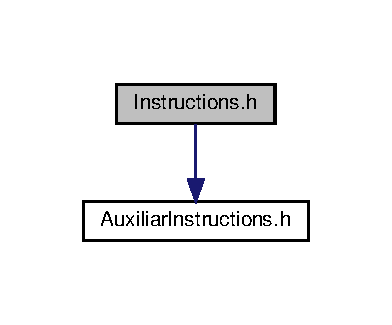
\includegraphics[width=260pt]{Instructions_8h__incl}
\end{center}
\end{figure}
Este grafo mostra quais arquivos estão direta ou indiretamente relacionados com este arquivo\+:\nopagebreak
\begin{figure}[H]
\begin{center}
\leavevmode
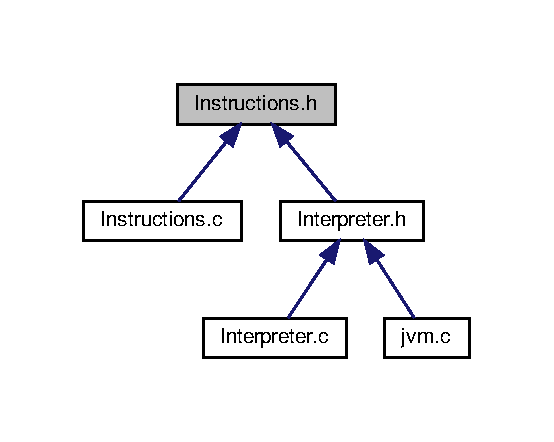
\includegraphics[width=266pt]{Instructions_8h__dep__incl}
\end{center}
\end{figure}
\subsection*{Definições e Macros}
\begin{DoxyCompactItemize}
\item 
\#define \hyperlink{Instructions_8h_a1884f9e9ef7c814e19cb7084fb7ccaa4}{S\+I\+Z\+E\+\_\+\+D\+O\+U\+B\+LE}~8
\end{DoxyCompactItemize}
\subsection*{Funções}
\begin{DoxyCompactItemize}
\item 
void \hyperlink{Instructions_8h_a705dd2fba1996967769549452c8266e1}{bipush} (char valor, \hyperlink{structFrameStack}{Frame\+Stack} $\ast$fs)
\begin{DoxyCompactList}\small\item\em Esta fun��o empilha um imediato de um byte. \end{DoxyCompactList}\item 
void \hyperlink{Instructions_8h_ac3b98fd98a5a66d5a193e31249f87ab5}{putstatic} (\hyperlink{structFrameStack}{Frame\+Stack} $\ast$fs)
\begin{DoxyCompactList}\small\item\em Esta fun��o desempilha o valor est�tico de um atributo de uma classe, e faz uma atribui��o ao campo. \end{DoxyCompactList}\item 
void \hyperlink{Instructions_8h_a9774fa7ccf4436f3bd486ecba45f7b72}{iconst} (\hyperlink{ClassLoader_8h_aedf6ddc03df8caaaccbb4c60b9a9b850}{u4} val, \hyperlink{structFrameStack}{Frame\+Stack} $\ast$fs)
\begin{DoxyCompactList}\small\item\em Esta função empilha um valor constante na pilha de operandos. \end{DoxyCompactList}\item 
void \hyperlink{Instructions_8h_a14ee4849c176450df2d8c109872abf7f}{istoren} (\hyperlink{ClassLoader_8h_aedf6ddc03df8caaaccbb4c60b9a9b850}{u4} val, \hyperlink{structFrameStack}{Frame\+Stack} $\ast$fs)
\begin{DoxyCompactList}\small\item\em Esta função simplesmente armazena um int do topo da pilha de operandos no vetor de variáveis locais. \end{DoxyCompactList}\item 
void \hyperlink{Instructions_8h_a49c874473ab4ef46868606485ee972c6}{iloadn} (\hyperlink{ClassLoader_8h_aedf6ddc03df8caaaccbb4c60b9a9b850}{u4} val, \hyperlink{structFrameStack}{Frame\+Stack} $\ast$fs)
\begin{DoxyCompactList}\small\item\em Esta função simplesmente carrega um int na pilha de operandos. \end{DoxyCompactList}\item 
void \hyperlink{Instructions_8h_add0fcbb1828f4213f1604c9d6305e9f0}{imul} (\hyperlink{structFrameStack}{Frame\+Stack} $\ast$fs)
\begin{DoxyCompactList}\small\item\em Esta função multiplica dois valores inteiros. \end{DoxyCompactList}\item 
void \hyperlink{Instructions_8h_a623503ebec3f0a1528a72dc4299d79db}{iadd} (\hyperlink{structFrameStack}{Frame\+Stack} $\ast$fs)
\begin{DoxyCompactList}\small\item\em Esta função soma dois valores inteiros. \end{DoxyCompactList}\item 
void \hyperlink{Instructions_8h_a9f7af649faabeddfda007b01ce895ba3}{isub} (\hyperlink{structFrameStack}{Frame\+Stack} $\ast$fs)
\begin{DoxyCompactList}\small\item\em Esta função subtrai dois valores inteiros. \end{DoxyCompactList}\item 
void \hyperlink{Instructions_8h_a4f9e7c6193392fe8824266697f51fcf5}{idiv} (\hyperlink{structFrameStack}{Frame\+Stack} $\ast$fs)
\begin{DoxyCompactList}\small\item\em Esta função divide dois valores inteiros. \end{DoxyCompactList}\item 
void \hyperlink{Instructions_8h_acfc35c6f495590de03ec16bb410fa2eb}{iand} (\hyperlink{structFrameStack}{Frame\+Stack} $\ast$fs)
\begin{DoxyCompactList}\small\item\em Esta função faz a operação \char`\"{}e\char`\"{} logico entre dois valores inteiros. \end{DoxyCompactList}\item 
void \hyperlink{Instructions_8h_a0a547b62f2d2962310ea9d0f77666a89}{ineg} (\hyperlink{structFrameStack}{Frame\+Stack} $\ast$fs)
\begin{DoxyCompactList}\small\item\em Esta função passa o valor para negativo de um inteiro. \end{DoxyCompactList}\item 
void \hyperlink{Instructions_8h_a90f4258b5f87aa1547bb969718ebd90e}{ior} (\hyperlink{structFrameStack}{Frame\+Stack} $\ast$fs)
\begin{DoxyCompactList}\small\item\em Esta função faz a operação \char`\"{}ou\char`\"{} logico entre dois valores inteiros. \end{DoxyCompactList}\item 
void \hyperlink{Instructions_8h_a6f1742a279efdafe9a8e35e0cfe70bc5}{ixor} (\hyperlink{structFrameStack}{Frame\+Stack} $\ast$fs)
\begin{DoxyCompactList}\small\item\em Esta função faz a operação logica \char`\"{}xor\char`\"{} entre dois valores inteiros. \end{DoxyCompactList}\item 
void \hyperlink{Instructions_8h_a5431f64e760037b20933b1ec0ff8c932}{irem} (\hyperlink{structFrameStack}{Frame\+Stack} $\ast$fs)
\begin{DoxyCompactList}\small\item\em Esta função pela o resto de uma divisão inteira. \end{DoxyCompactList}\item 
void \hyperlink{Instructions_8h_a5a47a84af9ce9210583e2b34e7e8ca17}{ishl} (\hyperlink{structFrameStack}{Frame\+Stack} $\ast$fs)
\begin{DoxyCompactList}\small\item\em Esta função faz o deslocamento de bits a esquerda de valores inteiros. \end{DoxyCompactList}\item 
void \hyperlink{Instructions_8h_ad7436a2936e0f5648f5e4341c51ebdcf}{ishr} (\hyperlink{structFrameStack}{Frame\+Stack} $\ast$fs)
\begin{DoxyCompactList}\small\item\em Esta função faz o deslocamento de bits a direita de valores inteiros. \end{DoxyCompactList}\item 
void \hyperlink{Instructions_8h_adf61ef75f4895aa3a4db1e3144a85816}{iushr} (\hyperlink{structFrameStack}{Frame\+Stack} $\ast$fs)
\begin{DoxyCompactList}\small\item\em Esta função faz o deslocamento de bits a direita de valores inteiros. \end{DoxyCompactList}\item 
void \hyperlink{Instructions_8h_a45ea65a52b6ea9e735727875934b8c47}{iload} (\hyperlink{structFrameStack}{Frame\+Stack} $\ast$fs)
\begin{DoxyCompactList}\small\item\em Esta função simplesmente carrega um int na pilha de operandos. \end{DoxyCompactList}\item 
void \hyperlink{Instructions_8h_a8c01e95c269879a1dc1a93334274b3a4}{istore} (\hyperlink{structFrameStack}{Frame\+Stack} $\ast$fs)
\begin{DoxyCompactList}\small\item\em Esta fun��o simplesmente armazena um int do topo da pilha de operandos no vetor de vari�veis locais. \end{DoxyCompactList}\item 
void \hyperlink{Instructions_8h_acb0bbb231bebfe7ee184f51439cde5a7}{iastore} (\hyperlink{structFrameStack}{Frame\+Stack} $\ast$fs)
\begin{DoxyCompactList}\small\item\em Esta função armazena um int do topo da pilha de operandos em um vetor de ints. \end{DoxyCompactList}\item 
void \hyperlink{Instructions_8h_a67421289339ff79e64120f6eece8f553}{i2l} (\hyperlink{structFrameStack}{Frame\+Stack} $\ast$fs)
\begin{DoxyCompactList}\small\item\em Esta funçao converte um int para long long. \end{DoxyCompactList}\item 
void \hyperlink{Instructions_8h_a289dc0bc8d211502c64e8eaf6c788891}{i2d} (\hyperlink{structFrameStack}{Frame\+Stack} $\ast$fs)
\begin{DoxyCompactList}\small\item\em Esta funçao converte um int para double. \end{DoxyCompactList}\item 
void \hyperlink{Instructions_8h_ae845ffb71260c681aef0497c9cc8c537}{i2c} (\hyperlink{structFrameStack}{Frame\+Stack} $\ast$fs)
\begin{DoxyCompactList}\small\item\em Esta funçao converte um int para char. \end{DoxyCompactList}\item 
void \hyperlink{Instructions_8h_a1b83b228e63c9d60057ddd3133ee95a3}{i2b} (\hyperlink{structFrameStack}{Frame\+Stack} $\ast$fs)
\begin{DoxyCompactList}\small\item\em Esta funçao converte um int para byte. \end{DoxyCompactList}\item 
void \hyperlink{Instructions_8h_a3dff2d25279d8cde9acba86e542960b8}{i2s} (\hyperlink{structFrameStack}{Frame\+Stack} $\ast$fs)
\begin{DoxyCompactList}\small\item\em Esta funçao converte um int para short. \end{DoxyCompactList}\item 
void \hyperlink{Instructions_8h_a701e241491f321212b2bec5be7f7e5b3}{lconstn} (long val1, \hyperlink{structFrameStack}{Frame\+Stack} $\ast$fs)
\begin{DoxyCompactList}\small\item\em Esta fun��o empilha um valor constante na pilha de operandos. \end{DoxyCompactList}\item 
void \hyperlink{Instructions_8h_ad864f908094892a5bd18dabc7c06d6c3}{lstoren} (\hyperlink{ClassLoader_8h_aedf6ddc03df8caaaccbb4c60b9a9b850}{u4} val, \hyperlink{structFrameStack}{Frame\+Stack} $\ast$fs)
\begin{DoxyCompactList}\small\item\em Esta função simplesmente armazena um long long do topo da pilha de operandos no vetor de variáveis locais. \end{DoxyCompactList}\item 
void \hyperlink{Instructions_8h_a79deb92ed9543e32e024835e7d195350}{lloadn} (\hyperlink{ClassLoader_8h_aedf6ddc03df8caaaccbb4c60b9a9b850}{u4} val, \hyperlink{structFrameStack}{Frame\+Stack} $\ast$fs)
\begin{DoxyCompactList}\small\item\em Esta função simplesmente carrega um long long na pilha de operandos. \end{DoxyCompactList}\item 
void \hyperlink{Instructions_8h_a6a53cc0354e8782ce6d8dd07219c96d5}{ladd} (\hyperlink{structFrameStack}{Frame\+Stack} $\ast$fs)
\begin{DoxyCompactList}\small\item\em Esta função soma dois valores long long. \end{DoxyCompactList}\item 
void \hyperlink{Instructions_8h_ac1c570a56086d685de552ede0f46d2f3}{lsub} (\hyperlink{structFrameStack}{Frame\+Stack} $\ast$fs)
\begin{DoxyCompactList}\small\item\em Esta função subtrai dois valores long long. \end{DoxyCompactList}\item 
void \hyperlink{Instructions_8h_a3dd414846c75f8b15a19b13e11c40fda}{lldiv\+\_\+} (\hyperlink{structFrameStack}{Frame\+Stack} $\ast$fs)
\begin{DoxyCompactList}\small\item\em Esta função divide dois valores long long. \end{DoxyCompactList}\item 
void \hyperlink{Instructions_8h_ac33a3332a30047f7da250f034c0bb9e5}{lrem} (\hyperlink{structFrameStack}{Frame\+Stack} $\ast$fs)
\begin{DoxyCompactList}\small\item\em Esta função divide dois valores long long e armazena o resto da divisao. \end{DoxyCompactList}\item 
void \hyperlink{Instructions_8h_a0ec203fbd351f0084818a871d92e6363}{lmul} (\hyperlink{structFrameStack}{Frame\+Stack} $\ast$fs)
\begin{DoxyCompactList}\small\item\em Esta função multiplicaçao dois valores long long. \end{DoxyCompactList}\item 
void \hyperlink{Instructions_8h_a1ccaa67537c2f37814764874da2aee04}{lneg} (\hyperlink{structFrameStack}{Frame\+Stack} $\ast$fs)
\begin{DoxyCompactList}\small\item\em Esta funçao passa o valor para negativo de um long long. \end{DoxyCompactList}\item 
void \hyperlink{Instructions_8h_af107187a6f0ab21fa07051bcce1fe477}{land} (\hyperlink{structFrameStack}{Frame\+Stack} $\ast$fs)
\begin{DoxyCompactList}\small\item\em Esta funçao faz a operaçao \char`\"{}e\char`\"{} logico entre dois valores long long. \end{DoxyCompactList}\item 
void \hyperlink{Instructions_8h_a5a7da23a7ecbd62acedc398f5295162c}{lor} (\hyperlink{structFrameStack}{Frame\+Stack} $\ast$fs)
\begin{DoxyCompactList}\small\item\em Esta funçao faz a operaçao \char`\"{}ou\char`\"{} logico entre dois valores long long. \end{DoxyCompactList}\item 
void \hyperlink{Instructions_8h_a1007ca19be5041d1fe3fbc71a621acfc}{lxor} (\hyperlink{structFrameStack}{Frame\+Stack} $\ast$fs)
\begin{DoxyCompactList}\small\item\em Esta funçao faz a operaçao \char`\"{}ou exclusivo\char`\"{} logico entre dois valores long long. \end{DoxyCompactList}\item 
void \hyperlink{Instructions_8h_a8ae75286fc4b426fcc7c7da53c93842c}{lshl} (\hyperlink{structFrameStack}{Frame\+Stack} $\ast$fs)
\begin{DoxyCompactList}\small\item\em Esta função faz o deslocamento de bits a esquerda de valores long long. \end{DoxyCompactList}\item 
void \hyperlink{Instructions_8h_a951fbc7756dfc4b798d531152a8fb93e}{lshr} (\hyperlink{structFrameStack}{Frame\+Stack} $\ast$fs)
\begin{DoxyCompactList}\small\item\em Esta função faz o deslocamento de bits a direita de valores long long. \end{DoxyCompactList}\item 
void \hyperlink{Instructions_8h_a5a3fa8102d08ff7db6556d4af5644f22}{lushr} (\hyperlink{structFrameStack}{Frame\+Stack} $\ast$fs)
\begin{DoxyCompactList}\small\item\em Esta função faz o deslocamento de bits a direita de valores long long. \end{DoxyCompactList}\item 
void \hyperlink{Instructions_8h_a1d0b49d57b4e97594a7f82bf299d487c}{lreturn} (\hyperlink{structFrameStack}{Frame\+Stack} $\ast$fs)
\begin{DoxyCompactList}\small\item\em Esta funçao executa o retorno de um metodo, empilhando o valor long long de retorno na pilha de operandos do frame do metodo chamador. \end{DoxyCompactList}\item 
void \hyperlink{Instructions_8h_a4e0a77edecb133b58f57ba29cd277b53}{l2d} (\hyperlink{structFrameStack}{Frame\+Stack} $\ast$fs)
\begin{DoxyCompactList}\small\item\em Esta funçao converte um long long para double. \end{DoxyCompactList}\item 
void \hyperlink{Instructions_8h_addaf018472ab2c5257e3275a50624818}{l2f} (\hyperlink{structFrameStack}{Frame\+Stack} $\ast$fs)
\begin{DoxyCompactList}\small\item\em Esta funçao converte um long long para float. \end{DoxyCompactList}\item 
void \hyperlink{Instructions_8h_a750239172914d03cc2a68608f545ecee}{l2i} (\hyperlink{structFrameStack}{Frame\+Stack} $\ast$fs)
\begin{DoxyCompactList}\small\item\em Esta funçao converte um long long para int. \end{DoxyCompactList}\item 
void \hyperlink{Instructions_8h_a8af416713ef811ca6cf0026c8a4b29b0}{lcmp} (\hyperlink{structFrameStack}{Frame\+Stack} $\ast$fs)
\begin{DoxyCompactList}\small\item\em Esta compara dois valores long long que estao no topo da pilha. \end{DoxyCompactList}\item 
void \hyperlink{Instructions_8h_a7022391b3bea98bf1e5537b195f789f5}{lload} (\hyperlink{structFrameStack}{Frame\+Stack} $\ast$fs)
\begin{DoxyCompactList}\small\item\em Esta função simplesmente carrega um long long na pilha de operandos. \end{DoxyCompactList}\item 
void \hyperlink{Instructions_8h_ad03163d48d68f24e57a5cbcf3159bac9}{fload} (\hyperlink{structFrameStack}{Frame\+Stack} $\ast$fs)
\begin{DoxyCompactList}\small\item\em Esta função simplesmente carrega um float na pilha de operandos. \end{DoxyCompactList}\item 
void \hyperlink{Instructions_8h_a3881f278d7316ed8e8853373b3c3d5fc}{floadn} (\hyperlink{ClassLoader_8h_aedf6ddc03df8caaaccbb4c60b9a9b850}{u4} val, \hyperlink{structFrameStack}{Frame\+Stack} $\ast$fs)
\begin{DoxyCompactList}\small\item\em Esta função simplesmente carrega uma constante float na pilha de operandos. \end{DoxyCompactList}\item 
void \hyperlink{Instructions_8h_a7e198a4137854449586d5d6bdbe360de}{lstore} (\hyperlink{structFrameStack}{Frame\+Stack} $\ast$fs)
\begin{DoxyCompactList}\small\item\em Esta funcao simplesmente armazena um long long do topo da pilha de operandos no vetor de variaveis locais. \end{DoxyCompactList}\item 
void \hyperlink{Instructions_8h_a03dd1a36cf9045704ce5867c540ac867}{lastore} (\hyperlink{structFrameStack}{Frame\+Stack} $\ast$fs)
\begin{DoxyCompactList}\small\item\em Esta função armazena um long long do topo da pilha de operandos em um vetor de long long\textquotesingle{}s. \end{DoxyCompactList}\item 
void \hyperlink{Instructions_8h_ab2e41bd12bf6cba5174c3ef2744b5388}{dconstn} (double val1, \hyperlink{structFrameStack}{Frame\+Stack} $\ast$fs)
\begin{DoxyCompactList}\small\item\em Esta fun��o empilha um valor constante na pilha de operandos. \end{DoxyCompactList}\item 
void \hyperlink{Instructions_8h_ac172c203901c8234b885afee1f2042cc}{dstoren} (\hyperlink{ClassLoader_8h_aedf6ddc03df8caaaccbb4c60b9a9b850}{u4} val, \hyperlink{structFrameStack}{Frame\+Stack} $\ast$fs)
\begin{DoxyCompactList}\small\item\em Esta função simplesmente armazena um double do topo da pilha de operandos no vetor de variáveis locais. \end{DoxyCompactList}\item 
void \hyperlink{Instructions_8h_a12bf774e8ddc18946ba4b94133d44546}{dloadn} (\hyperlink{ClassLoader_8h_aedf6ddc03df8caaaccbb4c60b9a9b850}{u4} val, \hyperlink{structFrameStack}{Frame\+Stack} $\ast$fs)
\begin{DoxyCompactList}\small\item\em Esta função simplesmente carrega um double na pilha de operandos. \end{DoxyCompactList}\item 
void \hyperlink{Instructions_8h_a7f2bfad7c28ae93c335c1c8616520d99}{dadd} (\hyperlink{structFrameStack}{Frame\+Stack} $\ast$fs)
\begin{DoxyCompactList}\small\item\em Esta função soma dois valores double. \end{DoxyCompactList}\item 
void \hyperlink{Instructions_8h_a6b3ca5eef979f4912636be9f8239049d}{dsub} (\hyperlink{structFrameStack}{Frame\+Stack} $\ast$fs)
\begin{DoxyCompactList}\small\item\em Esta função subtrai dois valores double. \end{DoxyCompactList}\item 
void \hyperlink{Instructions_8h_a8a8d2d455f2cbe8ba7d7ab735f5270b9}{ddiv} (\hyperlink{structFrameStack}{Frame\+Stack} $\ast$fs)
\begin{DoxyCompactList}\small\item\em Esta função divide dois valores double. \end{DoxyCompactList}\item 
void \hyperlink{Instructions_8h_a51cc19ebd5496bec721d27a4f6203f89}{d\+Rem} (\hyperlink{structFrameStack}{Frame\+Stack} $\ast$fs)
\begin{DoxyCompactList}\small\item\em Esta função divide dois valores double e armazena o resto da divisao. \end{DoxyCompactList}\item 
void \hyperlink{Instructions_8h_aa7135aa797378c29f558f804106f863b}{dmul} (\hyperlink{structFrameStack}{Frame\+Stack} $\ast$fs)
\begin{DoxyCompactList}\small\item\em Esta função multiplica dois valores double. \end{DoxyCompactList}\item 
void \hyperlink{Instructions_8h_aa8af81288ee43bca23c6a95d67ec1e23}{dneg} (\hyperlink{structFrameStack}{Frame\+Stack} $\ast$fs)
\begin{DoxyCompactList}\small\item\em Esta funçao passa o valor para negativo de um double. \end{DoxyCompactList}\item 
void \hyperlink{Instructions_8h_abbabf9264947f27e0ebeb39060b09448}{dcmpl} (\hyperlink{structFrameStack}{Frame\+Stack} $\ast$fs)
\begin{DoxyCompactList}\small\item\em Esta compara dois valores double que estao no topo da pilha. \end{DoxyCompactList}\item 
void \hyperlink{Instructions_8h_a4826f0038e41025231da4ce337e338d4}{dcmpg} (\hyperlink{structFrameStack}{Frame\+Stack} $\ast$fs)
\begin{DoxyCompactList}\small\item\em Esta � uma fun��o de compara��o de dois doubles da pilha de operandos utilizando o padr�o I\+E\+EE 754. \end{DoxyCompactList}\item 
void \hyperlink{Instructions_8h_acb76e47bacd394b13dce2820bb5fad9f}{dreturn} (\hyperlink{structFrameStack}{Frame\+Stack} $\ast$fs)
\begin{DoxyCompactList}\small\item\em Esta funçao executa o retorno de um metodo, empilhando o valor double de retorno na pilha de operandos do frame do metodo chamador. \end{DoxyCompactList}\item 
void \hyperlink{Instructions_8h_ad3f5e19e7279c969e5f69eeb7d2046f6}{d2l} (\hyperlink{structFrameStack}{Frame\+Stack} $\ast$fs)
\begin{DoxyCompactList}\small\item\em Esta funçao converte um double para long long. \end{DoxyCompactList}\item 
void \hyperlink{Instructions_8h_a4104b7156493ce1a5a02044a9d9a60ee}{d2f} (\hyperlink{structFrameStack}{Frame\+Stack} $\ast$fs)
\begin{DoxyCompactList}\small\item\em Esta funçao converte um double para float. \end{DoxyCompactList}\item 
void \hyperlink{Instructions_8h_a244d120a6e4bc0ca97ed598ce0b08bcb}{d2i} (\hyperlink{structFrameStack}{Frame\+Stack} $\ast$fs)
\begin{DoxyCompactList}\small\item\em Esta funçao converte um double para int. \end{DoxyCompactList}\item 
void \hyperlink{Instructions_8h_a10b33378017a94f7dfc03dd729ccd5b6}{dload} (\hyperlink{structFrameStack}{Frame\+Stack} $\ast$fs)
\begin{DoxyCompactList}\small\item\em Esta função simplesmente carrega um double na pilha de operandos. \end{DoxyCompactList}\item 
void \hyperlink{Instructions_8h_a8aa585d86f1ff8e6b9dec5285a33d9b6}{dstore} (\hyperlink{structFrameStack}{Frame\+Stack} $\ast$fs)
\begin{DoxyCompactList}\small\item\em Esta funcao simplesmente armazena um double do topo da pilha de operandos no vetor de variaveis locais. \end{DoxyCompactList}\item 
void \hyperlink{Instructions_8h_a65ff21c9bc7c3195d109a95721f56eca}{dastore} (\hyperlink{structFrameStack}{Frame\+Stack} $\ast$fs)
\begin{DoxyCompactList}\small\item\em Esta função armazena um double do topo da pilha de operandos em um vetor de long long\textquotesingle{}s. \end{DoxyCompactList}\item 
void \hyperlink{Instructions_8h_aaf33632fc01437bcca50421602ea5b1f}{dup} (\hyperlink{structFrameStack}{Frame\+Stack} $\ast$fs)
\begin{DoxyCompactList}\small\item\em Esta função faz o duplica o valor deo topo da pilha. \end{DoxyCompactList}\item 
void \hyperlink{Instructions_8h_aa91cf719e5339663a9fe5704b3e5bfe4}{dupx1} (\hyperlink{structFrameStack}{Frame\+Stack} $\ast$fs)
\begin{DoxyCompactList}\small\item\em Esta função duplica um valor intercalado a outro. \end{DoxyCompactList}\item 
void \hyperlink{Instructions_8h_a48f563018ce8aa6f43cbed7433a68a40}{dupx2\+\_\+1} (\hyperlink{structFrameStack}{Frame\+Stack} $\ast$fs)
\begin{DoxyCompactList}\small\item\em Esta função empilha valores no topo da pilha segundo uma determinada regra. \end{DoxyCompactList}\item 
void \hyperlink{Instructions_8h_a2dd2a6f684b065a929d4609b53422219}{dupx2\+\_\+2} (\hyperlink{structFrameStack}{Frame\+Stack} $\ast$fs)
\begin{DoxyCompactList}\small\item\em Esta função refaz a forma utilizada pela função dupx1. \end{DoxyCompactList}\item 
void \hyperlink{Instructions_8h_a5430b63fa308acbc720685f19e9b3617}{dup2} (\hyperlink{structFrameStack}{Frame\+Stack} $\ast$fs)
\begin{DoxyCompactList}\small\item\em Esta função empilha valores na pilha segundo uma determinada regra. \end{DoxyCompactList}\item 
void \hyperlink{Instructions_8h_a43d682b7080ee028515f377b3a28a076}{dup2x1\+\_\+1} (\hyperlink{structFrameStack}{Frame\+Stack} $\ast$fs)
\begin{DoxyCompactList}\small\item\em Esta função empilha valores na pilha segundo uma determinada regra. \end{DoxyCompactList}\item 
void \hyperlink{Instructions_8h_a5a1d5cb0adfea022d352ff5f5fe060b1}{dup2x1\+\_\+2} (\hyperlink{structFrameStack}{Frame\+Stack} $\ast$fs)
\begin{DoxyCompactList}\small\item\em Esta função refaz a forma utilizada pela função dupx1. \end{DoxyCompactList}\item 
void \hyperlink{Instructions_8h_aaf855a211029717dcc1b428d9889eef2}{dup2x2\+\_\+1} (\hyperlink{structFrameStack}{Frame\+Stack} $\ast$fs)
\begin{DoxyCompactList}\small\item\em Esta função empilha valores na pilha segundo uma determinada regra. \end{DoxyCompactList}\item 
void \hyperlink{Instructions_8h_a988cf09556fe8127cd2e088153832347}{dup2x2\+\_\+2} (\hyperlink{structFrameStack}{Frame\+Stack} $\ast$fs)
\begin{DoxyCompactList}\small\item\em Esta função empilha valores na pilha segundo uma determinada regra. \end{DoxyCompactList}\item 
void \hyperlink{Instructions_8h_a164222c1e344350279464e0557d7cc0f}{dup2x2\+\_\+3} (\hyperlink{structFrameStack}{Frame\+Stack} $\ast$fs)
\begin{DoxyCompactList}\small\item\em Esta função refaz a forma utilizada pela função dupx2x1\+\_\+1. \end{DoxyCompactList}\item 
void \hyperlink{Instructions_8h_a72541e2df41b1e9be9d36d4389a886b9}{dup2x2\+\_\+4} (\hyperlink{structFrameStack}{Frame\+Stack} $\ast$fs)
\begin{DoxyCompactList}\small\item\em Esta função refaz a forma utilizada pela função dupx1. \end{DoxyCompactList}\item 
void \hyperlink{Instructions_8h_a847f61be128bf30e88346cf55f7bc3ba}{frem} (\hyperlink{structFrameStack}{Frame\+Stack} $\ast$fs)
\begin{DoxyCompactList}\small\item\em Esta função obtém o resto de uma divisão de ponto flutuante. \end{DoxyCompactList}\item 
void \hyperlink{Instructions_8h_a026967129d62c77760656130595cacec}{fmul} (\hyperlink{structFrameStack}{Frame\+Stack} $\ast$fs)
\begin{DoxyCompactList}\small\item\em Esta função multiplica dois do tipo float. \end{DoxyCompactList}\item 
void \hyperlink{Instructions_8h_a778424f5d04a57b5c5b9c010b10642d3}{fneg} (\hyperlink{structFrameStack}{Frame\+Stack} $\ast$fs)
\begin{DoxyCompactList}\small\item\em Esta função passa o valor para negativo de um float. \end{DoxyCompactList}\item 
void \hyperlink{Instructions_8h_a34ecfdc9e3def3ee1fd4395cd45ba64c}{fconstn} (\hyperlink{ClassLoader_8h_aedf6ddc03df8caaaccbb4c60b9a9b850}{u4} val, \hyperlink{structFrameStack}{Frame\+Stack} $\ast$fs)
\begin{DoxyCompactList}\small\item\em Esta função insere na pilha um valor de ponto flutuante. \end{DoxyCompactList}\item 
void \hyperlink{Instructions_8h_a353f26708cd929278d61b6a6be8dee12}{fstore} (\hyperlink{structFrameStack}{Frame\+Stack} $\ast$fs)
\begin{DoxyCompactList}\small\item\em Esta função simplesmente armazena um float do topo da pilha de operandos no vetor de variáveis locais. \end{DoxyCompactList}\item 
void \hyperlink{Instructions_8h_a385c644c66d20927c82a9f19e7720a27}{fstoren} (\hyperlink{ClassLoader_8h_aedf6ddc03df8caaaccbb4c60b9a9b850}{u4} val, \hyperlink{structFrameStack}{Frame\+Stack} $\ast$fs)
\begin{DoxyCompactList}\small\item\em Esta função simplesmente armazena um float do topo da pilha de operandos no vetor de variáveis locais. \end{DoxyCompactList}\item 
void \hyperlink{Instructions_8h_a7a66351c38b630f31819190b8bd68f54}{fastore} (\hyperlink{structFrameStack}{Frame\+Stack} $\ast$fs)
\begin{DoxyCompactList}\small\item\em Esta função armazena um float do topo da pilha de operandos em um vetor de floats. \end{DoxyCompactList}\item 
void \hyperlink{Instructions_8h_a2fa2713004b611c8bc0bfebc89510ec0}{fadd} (\hyperlink{structFrameStack}{Frame\+Stack} $\ast$fs)
\begin{DoxyCompactList}\small\item\em Esta função soma dois valores do tipo float. \end{DoxyCompactList}\item 
void \hyperlink{Instructions_8h_ab5ddde2fa9a7480f08ccc33c4402a6c3}{fsub} (\hyperlink{structFrameStack}{Frame\+Stack} $\ast$fs)
\begin{DoxyCompactList}\small\item\em Esta função subtrai dois valores do tipo float. \end{DoxyCompactList}\item 
void \hyperlink{Instructions_8h_ada86d1da11dd35aac89d3e2be7cda5cf}{fdiv} (\hyperlink{structFrameStack}{Frame\+Stack} $\ast$fs)
\begin{DoxyCompactList}\small\item\em Esta função divide dois valores do tipo float. \end{DoxyCompactList}\item 
void \hyperlink{Instructions_8h_a1e6ace92acc086c83667982f68c2e448}{f2d} (\hyperlink{structFrameStack}{Frame\+Stack} $\ast$fs)
\begin{DoxyCompactList}\small\item\em Esta funçao converte um float para double. \end{DoxyCompactList}\item 
void \hyperlink{Instructions_8h_ad44b1dfb2457e7dde15873e44259bfd9}{f2i} (\hyperlink{structFrameStack}{Frame\+Stack} $\ast$fs)
\begin{DoxyCompactList}\small\item\em Esta funçao converte um float para int. \end{DoxyCompactList}\item 
void \hyperlink{Instructions_8h_a098f7408a3df0fd67ef07ee694cba314}{f2l} (\hyperlink{structFrameStack}{Frame\+Stack} $\ast$fs)
\begin{DoxyCompactList}\small\item\em Esta funçao converte um float para long long. \end{DoxyCompactList}\item 
void \hyperlink{Instructions_8h_a0f5d2ab60ed5197f3a3a3d1ee841dd8d}{sipush} (\hyperlink{structFrameStack}{Frame\+Stack} $\ast$fs)
\begin{DoxyCompactList}\small\item\em Esta fun��o simplesmente empilha um short (2 bytes) dado na pilha de operandos. \end{DoxyCompactList}\item 
void \hyperlink{Instructions_8h_a532851306e97050026eb46435c61e9cd}{ldc} (\hyperlink{structFrameStack}{Frame\+Stack} $\ast$fs)
\begin{DoxyCompactList}\small\item\em Esta fun��o busca uma constante no pool de constantes e a empilha na pilha de operandos. \end{DoxyCompactList}\item 
void \hyperlink{Instructions_8h_af89834744bb8c53ff1223c62af02df94}{ldc2} (\hyperlink{structFrameStack}{Frame\+Stack} $\ast$fs)
\begin{DoxyCompactList}\small\item\em Esta fun��o busca uma constante no pool de constantes e a empilha na pilha de operandos. \end{DoxyCompactList}\item 
void \hyperlink{Instructions_8h_a9758a41c86b5f83365c6d974f4464d6e}{aaload} (\hyperlink{structFrameStack}{Frame\+Stack} $\ast$fs)
\begin{DoxyCompactList}\small\item\em Esta fun��o armazena uma refer�ncia do topo da pilha de operandos em um vetor de refer�ncias. \end{DoxyCompactList}\item 
void \hyperlink{Instructions_8h_abf723135b1208847d159d47a54564595}{baload} (\hyperlink{structFrameStack}{Frame\+Stack} $\ast$fs)
\begin{DoxyCompactList}\small\item\em Esta fun��o empilha o valor em um dado �ndice de um array de bytes ou booleans na pilha de operandos, extendendo o sinal se a vari�vel for byte e n�o extendendo o sinal se a vari�vel for boolean. \end{DoxyCompactList}\item 
void \hyperlink{Instructions_8h_a3ba98d8f29fa2e335cedde2ee701dcfb}{iaload} (\hyperlink{structFrameStack}{Frame\+Stack} $\ast$fs)
\begin{DoxyCompactList}\small\item\em Esta fun��o armazena um int do topo da pilha de operandos em um vetor de ints. \end{DoxyCompactList}\item 
void \hyperlink{Instructions_8h_a93b5647880fca8535245cd71497a60b4}{laload} (\hyperlink{structFrameStack}{Frame\+Stack} $\ast$fs)
\begin{DoxyCompactList}\small\item\em Esta fun��o armazena um long long do topo da pilha de operandos em um vetor de long longs. \end{DoxyCompactList}\item 
void \hyperlink{Instructions_8h_a226b49b9de171996cf1f13360f65f0a6}{daload} (\hyperlink{structFrameStack}{Frame\+Stack} $\ast$fs)
\begin{DoxyCompactList}\small\item\em Esta fun��o armazena um double do topo da pilha de operandos em um vetor de doubles. \end{DoxyCompactList}\item 
void \hyperlink{Instructions_8h_a86a0cace7f3d67338e28486fe431f057}{caload} (\hyperlink{structFrameStack}{Frame\+Stack} $\ast$fs)
\begin{DoxyCompactList}\small\item\em Esta fun��o empilha o valor presente em um dado �ndice de um array de chars na pilha de operandos. \end{DoxyCompactList}\item 
void \hyperlink{Instructions_8h_a74f2eaf3d9a79736d123665b7e03ec13}{saload} (\hyperlink{structFrameStack}{Frame\+Stack} $\ast$fs)
\begin{DoxyCompactList}\small\item\em Esta fun��o armazena um short do topo da pilha de operandos em um vetor de shorts. \end{DoxyCompactList}\item 
void \hyperlink{Instructions_8h_a773dfc779489dc4e7749a29a499ed807}{faload} (\hyperlink{structFrameStack}{Frame\+Stack} $\ast$fs)
\begin{DoxyCompactList}\small\item\em Esta função carrega um float na pilha de operandos a partir de um array de floats. \end{DoxyCompactList}\item 
void \hyperlink{Instructions_8h_a88acb22190554ff72bc2b5a266f37c0b}{sastore} (\hyperlink{structFrameStack}{Frame\+Stack} $\ast$fs)
\begin{DoxyCompactList}\small\item\em Esta fun��o armazena um valor em um dado �ndice de um array de shorts. \end{DoxyCompactList}\item 
void \hyperlink{Instructions_8h_ac81420e277715c7a7ea2c82e6623b576}{castore} (\hyperlink{structFrameStack}{Frame\+Stack} $\ast$fs)
\begin{DoxyCompactList}\small\item\em Esta fun��o armazena um valor em um dado �ndice de um array de chars. \end{DoxyCompactList}\item 
void \hyperlink{Instructions_8h_a4384aded432d3ed9be44f92976708f2a}{aloadn} (\hyperlink{ClassLoader_8h_aedf6ddc03df8caaaccbb4c60b9a9b850}{u4} val, \hyperlink{structFrameStack}{Frame\+Stack} $\ast$fs)
\begin{DoxyCompactList}\small\item\em Esta fun��o empilha um valor do tipo refer�ncia armazenado em um certo �ndice do vetor de vari�veis locais na pilha de operandos. \end{DoxyCompactList}\item 
void \hyperlink{Instructions_8h_a5f0bee11c4a127ee1184c1f2472ee9b6}{astoren} (\hyperlink{ClassLoader_8h_a216a9f8b04b4f0af84a4ca9d1d85a6ca}{u1} val, \hyperlink{structFrameStack}{Frame\+Stack} $\ast$fs)
\begin{DoxyCompactList}\small\item\em Esta fun��o simplesmente armazena uma refer�ncia do topo da pilha de operandos no vetor de vari�veis locais. \end{DoxyCompactList}\item 
void \hyperlink{Instructions_8h_a8d96d1abf18ba97f8ec556fe5fe7cddf}{pop} (\hyperlink{structFrameStack}{Frame\+Stack} $\ast$fs)
\begin{DoxyCompactList}\small\item\em Esta função faz um pop na pilha de operandos. \end{DoxyCompactList}\item 
void \hyperlink{Instructions_8h_a66f881d94a0e1ebfcc247f3bdc62720f}{pop2} (\hyperlink{structFrameStack}{Frame\+Stack} $\ast$fs)
\begin{DoxyCompactList}\small\item\em Esta função faz dois pops na pilha de operandos. \end{DoxyCompactList}\item 
void \hyperlink{Instructions_8h_ae8c1c66e8119230a0245b76c42636f0c}{swap} (\hyperlink{structFrameStack}{Frame\+Stack} $\ast$fs)
\begin{DoxyCompactList}\small\item\em Esta função faz a troca de posição entre dois valores da pilha. \end{DoxyCompactList}\item 
void \hyperlink{Instructions_8h_ab8ac31bb6743ea143a088dd3a3f41c51}{iinc} (\hyperlink{structFrameStack}{Frame\+Stack} $\ast$fs)
\begin{DoxyCompactList}\small\item\em Esta fun��o simplesmente incrementa um valor do vetor de vari�veis locais. \end{DoxyCompactList}\item 
void \hyperlink{Instructions_8h_a4f64f89ab6d89fec030df9acc88b730d}{i2f} (\hyperlink{structFrameStack}{Frame\+Stack} $\ast$fs)
\begin{DoxyCompactList}\small\item\em Esta função coverte um valor inteiro para o tipo float. \end{DoxyCompactList}\item 
void \hyperlink{Instructions_8h_a8af59e9aec972bf0a8a4bca916e5e802}{fcmpl} (\hyperlink{structFrameStack}{Frame\+Stack} $\ast$fs)
\begin{DoxyCompactList}\small\item\em Esta é uma função de comparação de dois floats da pilha de operandos utilizando o padrão I\+E\+EE 754. \end{DoxyCompactList}\item 
void \hyperlink{Instructions_8h_a3819adbf3f5150e9a3ee9a6a13180a27}{fcmpg} (\hyperlink{structFrameStack}{Frame\+Stack} $\ast$fs)
\begin{DoxyCompactList}\small\item\em Esta � uma fun��o de compara��o de dois floats da pilha de operandos utilizando o padrão I\+E\+EE 754. \end{DoxyCompactList}\item 
void \hyperlink{Instructions_8h_ab97d9bee28ad74380ccf16fdb0891dec}{if\+\_\+icmpeq} (\hyperlink{structFrameStack}{Frame\+Stack} $\ast$fs)
\begin{DoxyCompactList}\small\item\em Esta fun��o compara os dois valores inteiros no topo da pilha de operandos, e calcula o offset a partir do qual PC deve ser incrementado para alcan�ar a pr�xima instru��o. \end{DoxyCompactList}\item 
void \hyperlink{Instructions_8h_a98218ae00da49f5e14d869765a1d430b}{if\+\_\+icmpne} (\hyperlink{structFrameStack}{Frame\+Stack} $\ast$fs)
\begin{DoxyCompactList}\small\item\em Esta fun��o compara os dois valores inteiros no topo da pilha de operandos, e calcula o offset a partir do qual PC deve ser incrementado para alcan�ar a pr�xima instru��o. \end{DoxyCompactList}\item 
void \hyperlink{Instructions_8h_a781631e63f47b9950053aca869f6beda}{if\+\_\+icmplt} (\hyperlink{structFrameStack}{Frame\+Stack} $\ast$fs)
\begin{DoxyCompactList}\small\item\em Esta fun��o compara se o valor no topo da pilha de operandos � maior que o segundo valor, e calcula o offset a partir do qual PC deve ser incrementado para alcan�ar a pr�xima instru��o. \end{DoxyCompactList}\item 
void \hyperlink{Instructions_8h_a984ee14a3d1305398a30d71a39a31e2b}{if\+\_\+icmpge} (\hyperlink{structFrameStack}{Frame\+Stack} $\ast$fs)
\begin{DoxyCompactList}\small\item\em Esta fun��o retira dois elementos do topo da pilha, e calcula um offset a partir do qual PC deve ser incrementado para alcan�ar a pr�xima instru��o. \end{DoxyCompactList}\item 
void \hyperlink{Instructions_8h_aaf08c7dcf4830be0ca8c009322d7afa8}{if\+\_\+icmpgt} (\hyperlink{structFrameStack}{Frame\+Stack} $\ast$fs)
\begin{DoxyCompactList}\small\item\em Esta fun��o retira dois elementos do topo da pilha, e produz um offset a partir do qual PC deve ser incrementado para alcan�ar a pr�xima instru��o. \end{DoxyCompactList}\item 
void \hyperlink{Instructions_8h_a4661a511019cc319a25485bbb060da36}{if\+\_\+icmple} (\hyperlink{structFrameStack}{Frame\+Stack} $\ast$fs)
\begin{DoxyCompactList}\small\item\em Esta fun��o compara se o valor no topo da pilha de operandos � maior ou igual ao segundo valor, e calcula o offset a partir do qual PC deve ser incrementado para alcan�ar a pr�xima instru��o. \end{DoxyCompactList}\item 
void \hyperlink{Instructions_8h_ab1f6e9da234a92f5725f6c0de3c47a39}{Goto} (\hyperlink{structFrameStack}{Frame\+Stack} $\ast$fs)
\begin{DoxyCompactList}\small\item\em Esta fun��o produz um deslocamento de 16 bits a ser somado ao valor de PC para implementar um desvio incondicional. \end{DoxyCompactList}\item 
void \hyperlink{Instructions_8h_a61f19fe1ba20edb901a2090344a983de}{Goto\+\_\+w} (\hyperlink{structFrameStack}{Frame\+Stack} $\ast$fs)
\begin{DoxyCompactList}\small\item\em Esta fun��o produz um deslocamento de 32 bits a ser somado ao valor de PC para implementar um desvio incondicional. \end{DoxyCompactList}\item 
void \hyperlink{Instructions_8h_af705acf601f1223a0f9f7e839d6a16ed}{ireturn} (\hyperlink{structFrameStack}{Frame\+Stack} $\ast$fs)
\begin{DoxyCompactList}\small\item\em Esta funçao executa o retorno de um metodo, empilhando o valor int de retorno na pilha de operandos do frame do metodo chamador. \end{DoxyCompactList}\item 
void \hyperlink{Instructions_8h_a8a6f8d2ae4502435cf6c67fdfe83543e}{freturn} (\hyperlink{structFrameStack}{Frame\+Stack} $\ast$fs)
\begin{DoxyCompactList}\small\item\em Esta fun��o executa o retorno de um metodo, empilhando o valor float de retorno na pilha de operandos do frame do metodo chamador. \end{DoxyCompactList}\item 
void \hyperlink{Instructions_8h_a25e65a9f93b6628203beed5f4a3d542a}{aload} (\hyperlink{structFrameStack}{Frame\+Stack} $\ast$fs)
\begin{DoxyCompactList}\small\item\em Esta fun��o faz um push de uma referencia no frame que est� na pilha de frame. \end{DoxyCompactList}\item 
void \hyperlink{Instructions_8h_acfb54f8f70bbbc2e8dfc91a9f4d6b0bd}{astore} (\hyperlink{structFrameStack}{Frame\+Stack} $\ast$fs)
\begin{DoxyCompactList}\small\item\em Esta fun��o faz um pop de uma referencia no frame que est� na pilha de frame. \end{DoxyCompactList}\item 
void \hyperlink{Instructions_8h_a025278966d6ee63ae872e680a1827eb4}{anewarray} (\hyperlink{structFrameStack}{Frame\+Stack} $\ast$fs)
\item 
void \hyperlink{Instructions_8h_ad0af00102fb7621045a1c6035acfe5eb}{getstatic} (\hyperlink{structFrameStack}{Frame\+Stack} $\ast$fs)
\begin{DoxyCompactList}\small\item\em Esta fun��o coloca no frame o operador est�tico. \end{DoxyCompactList}\item 
void \hyperlink{Instructions_8h_aec146b3cfa3d34b7d6804d574c80636e}{newarray} (\hyperlink{structFrameStack}{Frame\+Stack} $\ast$fs)
\begin{DoxyCompactList}\small\item\em Esta fun��o empilha a refer�ncia e aloca a mem�ria para um array unidimensional. \end{DoxyCompactList}\item 
void \hyperlink{Instructions_8h_a4d1a81a0faca488a7f82de6a5576d4e1}{multianewarray} (\hyperlink{structFrameStack}{Frame\+Stack} $\ast$fs)
\begin{DoxyCompactList}\small\item\em Esta fun��o empilha a refer�ncia e aloca a mem�ria para um array multidimensional. \end{DoxyCompactList}\item 
void \hyperlink{Instructions_8h_a7e9f3a9b0d70c7453f8e234f2483d4c8}{new\+Obj} (\hyperlink{structFrameStack}{Frame\+Stack} $\ast$fs)
\begin{DoxyCompactList}\small\item\em Esta fun��o procura a classe e cria um novo objeto dessa classe. \end{DoxyCompactList}\item 
\hyperlink{structarrayMult}{array\+Mult} $\ast$ \hyperlink{Instructions_8h_a1a30209ee66bb49b17a547b06e41d6d5}{Reduce\+Dimension} (\hyperlink{structarrayMult}{array\+Mult} $\ast$dimen, \hyperlink{ClassLoader_8h_aedf6ddc03df8caaaccbb4c60b9a9b850}{u4} qualpos)
\begin{DoxyCompactList}\small\item\em Esta fun��o reduz uma �nica dimens�o do array multidimensional. \end{DoxyCompactList}\item 
void \hyperlink{Instructions_8h_aaf568b4090e91eb7bab05d285a05c494}{areturn} (\hyperlink{structFrameStack}{Frame\+Stack} $\ast$fs)
\begin{DoxyCompactList}\small\item\em Esta fun��o retorna uma refer�ncia. \end{DoxyCompactList}\item 
void \hyperlink{Instructions_8h_a7d28c1bcf59ba303119001f847b64a6d}{aconstnull} (\hyperlink{structFrameStack}{Frame\+Stack} $\ast$fs)
\begin{DoxyCompactList}\small\item\em Esta fun��o emplilha um ponteiro com o valor null. \end{DoxyCompactList}\item 
void \hyperlink{Instructions_8h_abea004772e0d61315aceb30738629b69}{bastore} (\hyperlink{structFrameStack}{Frame\+Stack} $\ast$fs)
\begin{DoxyCompactList}\small\item\em Esta fun��o armazena um valor em um dado �ndice de um array de byte ou boolean. \end{DoxyCompactList}\item 
void \hyperlink{Instructions_8h_a58eac8eff63f9b01d3e732868752d29d}{getfield} (\hyperlink{structFrameStack}{Frame\+Stack} $\ast$fs)
\begin{DoxyCompactList}\small\item\em Esta fun��o empilha o valor de um atributo de uma classe. \end{DoxyCompactList}\item 
void \hyperlink{Instructions_8h_a973ed81061aab3cc555c3e81e1d96edf}{putfield} (\hyperlink{structFrameStack}{Frame\+Stack} $\ast$fs)
\begin{DoxyCompactList}\small\item\em Esta fun��o desempilha o valor de um atributo de uma classe, e faz uma atribui��o ao campo. \end{DoxyCompactList}\item 
void \hyperlink{Instructions_8h_aee7559362b17e07327f743f0bec3afd6}{ifeq} (\hyperlink{structFrameStack}{Frame\+Stack} $\ast$fs)
\begin{DoxyCompactList}\small\item\em Esta fun��o implementa um desvio condicional do tipo vari�vel igual a zero, calculando um deslocamento a ser adicionado ao valor de PC para alcan�ar a pr�xima instru��o. \end{DoxyCompactList}\item 
void \hyperlink{Instructions_8h_aaedd51dc94e53861a357b9df3754aa66}{ifne} (\hyperlink{structFrameStack}{Frame\+Stack} $\ast$fs)
\begin{DoxyCompactList}\small\item\em Esta fun��o implementa um desvio condicional do tipo vari�vel diferente de zero, calculando um deslocamento a ser adicionado ao valor de PC para alcan�ar a pr�xima instru��o. \end{DoxyCompactList}\item 
void \hyperlink{Instructions_8h_ad504c74f331058c5f95a9ac7ff9d18e1}{iflt} (\hyperlink{structFrameStack}{Frame\+Stack} $\ast$fs)
\begin{DoxyCompactList}\small\item\em Esta fun��o implementa um desvio condicional do tipo vari�vel menor que zero, calculando um deslocamento a ser adicionado ao valor de PC para alcan�ar a pr�xima instru��o. \end{DoxyCompactList}\item 
void \hyperlink{Instructions_8h_aeb8800de8baa55ab71d6cb58fc93c22b}{ifle} (\hyperlink{structFrameStack}{Frame\+Stack} $\ast$fs)
\begin{DoxyCompactList}\small\item\em Esta fun��o implementa um desvio condicional do tipo vari�vel menor ou igual a zero, calculando um deslocamento a ser adicionado ao valor de PC para alcan�ar a pr�xima instru��o. \end{DoxyCompactList}\item 
void \hyperlink{Instructions_8h_ac1c65e20772cf0ea744a4615fe38a388}{ifgt} (\hyperlink{structFrameStack}{Frame\+Stack} $\ast$fs)
\begin{DoxyCompactList}\small\item\em Esta fun��o implementa um desvio condicional do tipo vari�vel maior que zero, calculando um deslocamento a ser adicionado ao valor de PC para alcan�ar a pr�xima instru��o. \end{DoxyCompactList}\item 
void \hyperlink{Instructions_8h_abf549ebd8ac5fed66d6678af96f1f062}{ifge} (\hyperlink{structFrameStack}{Frame\+Stack} $\ast$fs)
\begin{DoxyCompactList}\small\item\em Esta fun��o implementa um desvio condicional do tipo vari�vel maior ou igual a zero, calculando um deslocamento a ser adicionado ao valor de PC para alcan�ar a pr�xima instru��o. \end{DoxyCompactList}\item 
void \hyperlink{Instructions_8h_a415c81a41fac4524d110aff25284830e}{if\+\_\+acmpeq} (\hyperlink{structFrameStack}{Frame\+Stack} $\ast$fs)
\begin{DoxyCompactList}\small\item\em Esta fun��o compara os dois valores do tipo refer�ncia no topo da pilha de operandos, e produz o offset a partir do qual PC deve ser incrementado para alcan�ar a pr�xima instru��o. \end{DoxyCompactList}\item 
void \hyperlink{Instructions_8h_a35f02117ec35a53434035688c339a21f}{if\+\_\+acmpne} (\hyperlink{structFrameStack}{Frame\+Stack} $\ast$fs)
\begin{DoxyCompactList}\small\item\em Esta fun��o compara os dois valores do tipo refer�ncia no topo da pilha de operandos, e produz o offset a partir do qual PC deve ser incrementado para alcan�ar a pr�xima instru��o. \end{DoxyCompactList}\item 
void \hyperlink{Instructions_8h_ae010f8139df37446a351566312688379}{jsr} (\hyperlink{structFrameStack}{Frame\+Stack} $\ast$fs)
\begin{DoxyCompactList}\small\item\em Esta fun��o empilha o endere�o da pr�xima execu��o a ser executada e retorna um deslocamento de 16 bits a ser somado a PC. \end{DoxyCompactList}\item 
void \hyperlink{Instructions_8h_a17d3e3e5fb8d99e25a1e5caf899c54a1}{jsr\+\_\+w} (\hyperlink{structFrameStack}{Frame\+Stack} $\ast$fs)
\begin{DoxyCompactList}\small\item\em Esta fun��o empilha o endere�o da pr�xima execu��o a ser executada e retorna um deslocamento de 32 bits a ser somado a PC. \end{DoxyCompactList}\item 
void \hyperlink{Instructions_8h_a68fc171934ce61f90c721103e173905d}{ret} (\hyperlink{structFrameStack}{Frame\+Stack} $\ast$fs)
\begin{DoxyCompactList}\small\item\em Esta fun��o l� o novo ppc do vetor de vari�veis locais. \end{DoxyCompactList}\item 
void \hyperlink{Instructions_8h_ac1a0c8fff689e07ee131622c5717132e}{ifnull} (\hyperlink{structFrameStack}{Frame\+Stack} $\ast$fs)
\begin{DoxyCompactList}\small\item\em Esta fun��o verifica se o valor no topo da pilha � uma refer�ncia nula, e produz um offset a ser somado ao PC para alcan�ar a pr�xima instru��o a ser executada. \end{DoxyCompactList}\item 
void \hyperlink{Instructions_8h_a12dec4bc7993af7347d0f46e20d6c6e7}{ifnonull} (\hyperlink{structFrameStack}{Frame\+Stack} $\ast$fs)
\begin{DoxyCompactList}\small\item\em Esta fun��o verifica se o valor no topo da pilha � uma refer�ncia nula, e produz um offset a ser somado ao PC para alcan�ar a pr�xima instru��o a ser executada. \end{DoxyCompactList}\item 
void \hyperlink{Instructions_8h_a8475bd26f5f967d5e3a7cd972179acc2}{tableswitch} (\hyperlink{structFrameStack}{Frame\+Stack} $\ast$fs)
\begin{DoxyCompactList}\small\item\em Esta fun��o que executa o comando switch. \end{DoxyCompactList}\end{DoxyCompactItemize}


\subsection{Definições e macros}
\mbox{\Hypertarget{Instructions_8h_a1884f9e9ef7c814e19cb7084fb7ccaa4}\label{Instructions_8h_a1884f9e9ef7c814e19cb7084fb7ccaa4}} 
\index{Instructions.\+h@{Instructions.\+h}!S\+I\+Z\+E\+\_\+\+D\+O\+U\+B\+LE@{S\+I\+Z\+E\+\_\+\+D\+O\+U\+B\+LE}}
\index{S\+I\+Z\+E\+\_\+\+D\+O\+U\+B\+LE@{S\+I\+Z\+E\+\_\+\+D\+O\+U\+B\+LE}!Instructions.\+h@{Instructions.\+h}}
\subsubsection{\texorpdfstring{S\+I\+Z\+E\+\_\+\+D\+O\+U\+B\+LE}{SIZE\_DOUBLE}}
{\footnotesize\ttfamily \#define S\+I\+Z\+E\+\_\+\+D\+O\+U\+B\+LE~8}



\subsection{Funções}
\mbox{\Hypertarget{Instructions_8h_a9758a41c86b5f83365c6d974f4464d6e}\label{Instructions_8h_a9758a41c86b5f83365c6d974f4464d6e}} 
\index{Instructions.\+h@{Instructions.\+h}!aaload@{aaload}}
\index{aaload@{aaload}!Instructions.\+h@{Instructions.\+h}}
\subsubsection{\texorpdfstring{aaload()}{aaload()}}
{\footnotesize\ttfamily void aaload (\begin{DoxyParamCaption}\item[{\hyperlink{structFrameStack}{Frame\+Stack} $\ast$}]{fs }\end{DoxyParamCaption})}



Esta fun��o armazena uma refer�ncia do topo da pilha de operandos em um vetor de refer�ncias. 

A fun��o retira da pilha de operandos o valor da refer�ncia a ser armazenado do vetor, o �ndice para a posi��o onde esse elemento ser� armazenado e uma refer�ncia a posi��o do in�cio desse vetor na mem�ria 
\begin{DoxyParams}{Parâmetros}
{\em $\ast$fs} & O ponteiro para o frame. \\
\hline
\end{DoxyParams}
\mbox{\Hypertarget{Instructions_8h_a7d28c1bcf59ba303119001f847b64a6d}\label{Instructions_8h_a7d28c1bcf59ba303119001f847b64a6d}} 
\index{Instructions.\+h@{Instructions.\+h}!aconstnull@{aconstnull}}
\index{aconstnull@{aconstnull}!Instructions.\+h@{Instructions.\+h}}
\subsubsection{\texorpdfstring{aconstnull()}{aconstnull()}}
{\footnotesize\ttfamily void aconstnull (\begin{DoxyParamCaption}\item[{\hyperlink{structFrameStack}{Frame\+Stack} $\ast$}]{fs }\end{DoxyParamCaption})}



Esta fun��o emplilha um ponteiro com o valor null. 


\begin{DoxyParams}{Parâmetros}
{\em $\ast$fs} & O frame onde a opera��o � executada. \\
\hline
\end{DoxyParams}
\mbox{\Hypertarget{Instructions_8h_a25e65a9f93b6628203beed5f4a3d542a}\label{Instructions_8h_a25e65a9f93b6628203beed5f4a3d542a}} 
\index{Instructions.\+h@{Instructions.\+h}!aload@{aload}}
\index{aload@{aload}!Instructions.\+h@{Instructions.\+h}}
\subsubsection{\texorpdfstring{aload()}{aload()}}
{\footnotesize\ttfamily void aload (\begin{DoxyParamCaption}\item[{\hyperlink{structFrameStack}{Frame\+Stack} $\ast$}]{fs }\end{DoxyParamCaption})}



Esta fun��o faz um push de uma referencia no frame que est� na pilha de frame. 


\begin{DoxyParams}{Parâmetros}
{\em $\ast$fs} & O ponteiro para o frame. \\
\hline
\end{DoxyParams}
\mbox{\Hypertarget{Instructions_8h_a4384aded432d3ed9be44f92976708f2a}\label{Instructions_8h_a4384aded432d3ed9be44f92976708f2a}} 
\index{Instructions.\+h@{Instructions.\+h}!aloadn@{aloadn}}
\index{aloadn@{aloadn}!Instructions.\+h@{Instructions.\+h}}
\subsubsection{\texorpdfstring{aloadn()}{aloadn()}}
{\footnotesize\ttfamily void aloadn (\begin{DoxyParamCaption}\item[{\hyperlink{ClassLoader_8h_aedf6ddc03df8caaaccbb4c60b9a9b850}{u4}}]{val,  }\item[{\hyperlink{structFrameStack}{Frame\+Stack} $\ast$}]{fs }\end{DoxyParamCaption})}



Esta fun��o empilha um valor do tipo refer�ncia armazenado em um certo �ndice do vetor de vari�veis locais na pilha de operandos. 

Esta fun��o na verdade implementa a fam�lia de instru��es aload\+\_\+$<$n$>$ onde n varia de 0 a 3 inclusive. 
\begin{DoxyParams}{Parâmetros}
{\em $\ast$fs} & O ponteiro para o frame onde se executar� a opera��o. \\
\hline
{\em val} & O �ndice no vetor de vari�veis locais onde o valor do tipo refer�ncia est� armazenado. \\
\hline
\end{DoxyParams}
\mbox{\Hypertarget{Instructions_8h_a025278966d6ee63ae872e680a1827eb4}\label{Instructions_8h_a025278966d6ee63ae872e680a1827eb4}} 
\index{Instructions.\+h@{Instructions.\+h}!anewarray@{anewarray}}
\index{anewarray@{anewarray}!Instructions.\+h@{Instructions.\+h}}
\subsubsection{\texorpdfstring{anewarray()}{anewarray()}}
{\footnotesize\ttfamily void anewarray (\begin{DoxyParamCaption}\item[{\hyperlink{structFrameStack}{Frame\+Stack} $\ast$}]{fs }\end{DoxyParamCaption})}

\mbox{\Hypertarget{Instructions_8h_aaf568b4090e91eb7bab05d285a05c494}\label{Instructions_8h_aaf568b4090e91eb7bab05d285a05c494}} 
\index{Instructions.\+h@{Instructions.\+h}!areturn@{areturn}}
\index{areturn@{areturn}!Instructions.\+h@{Instructions.\+h}}
\subsubsection{\texorpdfstring{areturn()}{areturn()}}
{\footnotesize\ttfamily void areturn (\begin{DoxyParamCaption}\item[{\hyperlink{structFrameStack}{Frame\+Stack} $\ast$}]{fs }\end{DoxyParamCaption})}



Esta fun��o retorna uma refer�ncia. 


\begin{DoxyParams}{Parâmetros}
{\em $\ast$fs} & O frame onde a opera��o � executada. \\
\hline
\end{DoxyParams}
\mbox{\Hypertarget{Instructions_8h_acfb54f8f70bbbc2e8dfc91a9f4d6b0bd}\label{Instructions_8h_acfb54f8f70bbbc2e8dfc91a9f4d6b0bd}} 
\index{Instructions.\+h@{Instructions.\+h}!astore@{astore}}
\index{astore@{astore}!Instructions.\+h@{Instructions.\+h}}
\subsubsection{\texorpdfstring{astore()}{astore()}}
{\footnotesize\ttfamily void astore (\begin{DoxyParamCaption}\item[{\hyperlink{structFrameStack}{Frame\+Stack} $\ast$}]{fs }\end{DoxyParamCaption})}



Esta fun��o faz um pop de uma referencia no frame que est� na pilha de frame. 


\begin{DoxyParams}{Parâmetros}
{\em $\ast$fs} & O ponteiro para o frame. \\
\hline
\end{DoxyParams}
\mbox{\Hypertarget{Instructions_8h_a5f0bee11c4a127ee1184c1f2472ee9b6}\label{Instructions_8h_a5f0bee11c4a127ee1184c1f2472ee9b6}} 
\index{Instructions.\+h@{Instructions.\+h}!astoren@{astoren}}
\index{astoren@{astoren}!Instructions.\+h@{Instructions.\+h}}
\subsubsection{\texorpdfstring{astoren()}{astoren()}}
{\footnotesize\ttfamily void astoren (\begin{DoxyParamCaption}\item[{\hyperlink{ClassLoader_8h_a216a9f8b04b4f0af84a4ca9d1d85a6ca}{u1}}]{val,  }\item[{\hyperlink{structFrameStack}{Frame\+Stack} $\ast$}]{fs }\end{DoxyParamCaption})}



Esta fun��o simplesmente armazena uma refer�ncia do topo da pilha de operandos no vetor de vari�veis locais. 

A fun��o primeiro desempilha o valor do topo da pilha e esse valor � armazenado no vetor de vari�veis locais na posi��o indicada por �ndice. 
\begin{DoxyParams}{Parâmetros}
{\em $\ast$fs} & O ponteiro para o frame. \\
\hline
{\em val} & O �ndice indicando a posi��o do vetor de vari�veis locais onde a refer�ncia ser� armazenada. \\
\hline
\end{DoxyParams}
\mbox{\Hypertarget{Instructions_8h_abf723135b1208847d159d47a54564595}\label{Instructions_8h_abf723135b1208847d159d47a54564595}} 
\index{Instructions.\+h@{Instructions.\+h}!baload@{baload}}
\index{baload@{baload}!Instructions.\+h@{Instructions.\+h}}
\subsubsection{\texorpdfstring{baload()}{baload()}}
{\footnotesize\ttfamily void baload (\begin{DoxyParamCaption}\item[{\hyperlink{structFrameStack}{Frame\+Stack} $\ast$}]{fs }\end{DoxyParamCaption})}



Esta fun��o empilha o valor em um dado �ndice de um array de bytes ou booleans na pilha de operandos, extendendo o sinal se a vari�vel for byte e n�o extendendo o sinal se a vari�vel for boolean. 

A fun��o opera desempilhando o �ndice e o endere�o do vetor da pilha de operandos, ap�s isso o endere�o do vetor � copiado para um ponteiro para a estrutura array. O tipo do vetor � determinado, se for byte o valor naquele �ndice do vetor tem seu sinal extendido para 32 bits e armazenado na pilha de operandos. Caso o tipo do vetor seja boolean o valor naquela posi��o � empilhado na pilha de operandos, sem extens�o de sinal. 
\begin{DoxyParams}{Parâmetros}
{\em $\ast$fs} & O ponteiro para a pilha de frames. \\
\hline
\end{DoxyParams}
\mbox{\Hypertarget{Instructions_8h_abea004772e0d61315aceb30738629b69}\label{Instructions_8h_abea004772e0d61315aceb30738629b69}} 
\index{Instructions.\+h@{Instructions.\+h}!bastore@{bastore}}
\index{bastore@{bastore}!Instructions.\+h@{Instructions.\+h}}
\subsubsection{\texorpdfstring{bastore()}{bastore()}}
{\footnotesize\ttfamily void bastore (\begin{DoxyParamCaption}\item[{\hyperlink{structFrameStack}{Frame\+Stack} $\ast$}]{fs }\end{DoxyParamCaption})}



Esta fun��o armazena um valor em um dado �ndice de um array de byte ou boolean. 

A fun��o opera desempilhando o valor a ser armazenado no vetor, o �ndice a ser alterado e a refer�ncia para o array de bytes ou booleans. Ap�s isso o valor desempilhado � armazenado naquele �ndice do array. 
\begin{DoxyParams}{Parâmetros}
{\em $\ast$fs} & O ponteiro para o frame onde se efetuar� a opera��o. \\
\hline
\end{DoxyParams}
\mbox{\Hypertarget{Instructions_8h_a705dd2fba1996967769549452c8266e1}\label{Instructions_8h_a705dd2fba1996967769549452c8266e1}} 
\index{Instructions.\+h@{Instructions.\+h}!bipush@{bipush}}
\index{bipush@{bipush}!Instructions.\+h@{Instructions.\+h}}
\subsubsection{\texorpdfstring{bipush()}{bipush()}}
{\footnotesize\ttfamily void bipush (\begin{DoxyParamCaption}\item[{char}]{valor,  }\item[{\hyperlink{structFrameStack}{Frame\+Stack} $\ast$}]{fs }\end{DoxyParamCaption})}



Esta fun��o empilha um imediato de um byte. 

A fun��o opera inserindo um valor byte no topo do pilha 
\begin{DoxyParams}{Parâmetros}
{\em valor} & Um byte a ser empilhado. \\
\hline
{\em $\ast$fs} & O ponteiro para o frame. \\
\hline
\end{DoxyParams}
\mbox{\Hypertarget{Instructions_8h_a86a0cace7f3d67338e28486fe431f057}\label{Instructions_8h_a86a0cace7f3d67338e28486fe431f057}} 
\index{Instructions.\+h@{Instructions.\+h}!caload@{caload}}
\index{caload@{caload}!Instructions.\+h@{Instructions.\+h}}
\subsubsection{\texorpdfstring{caload()}{caload()}}
{\footnotesize\ttfamily void caload (\begin{DoxyParamCaption}\item[{\hyperlink{structFrameStack}{Frame\+Stack} $\ast$}]{fs }\end{DoxyParamCaption})}



Esta fun��o empilha o valor presente em um dado �ndice de um array de chars na pilha de operandos. 

A fun��o opera desempilhando um �ndice e uma refer�ncia para um array de chars, buscando o valor presente naquele �ndice do array, e empilhando esse valor na pilha de operandos. 
\begin{DoxyParams}{Parâmetros}
{\em $\ast$fs} & O ponteiro para o frame onde a opera��o � executada. \\
\hline
\end{DoxyParams}
\mbox{\Hypertarget{Instructions_8h_ac81420e277715c7a7ea2c82e6623b576}\label{Instructions_8h_ac81420e277715c7a7ea2c82e6623b576}} 
\index{Instructions.\+h@{Instructions.\+h}!castore@{castore}}
\index{castore@{castore}!Instructions.\+h@{Instructions.\+h}}
\subsubsection{\texorpdfstring{castore()}{castore()}}
{\footnotesize\ttfamily void castore (\begin{DoxyParamCaption}\item[{\hyperlink{structFrameStack}{Frame\+Stack} $\ast$}]{fs }\end{DoxyParamCaption})}



Esta fun��o armazena um valor em um dado �ndice de um array de chars. 

A fun��o opera desempilhando o valor a ser armazenado no vetor, o �ndice a ser alterado e a refer�ncia para o array de chars. Ap�s isso o valor desempilhado � armazenado naquele �ndice do array. 
\begin{DoxyParams}{Parâmetros}
{\em $\ast$fs} & O ponteiro para o frame onde se efetuar� a opera��o. \\
\hline
\end{DoxyParams}
\mbox{\Hypertarget{Instructions_8h_a4104b7156493ce1a5a02044a9d9a60ee}\label{Instructions_8h_a4104b7156493ce1a5a02044a9d9a60ee}} 
\index{Instructions.\+h@{Instructions.\+h}!d2f@{d2f}}
\index{d2f@{d2f}!Instructions.\+h@{Instructions.\+h}}
\subsubsection{\texorpdfstring{d2f()}{d2f()}}
{\footnotesize\ttfamily void d2f (\begin{DoxyParamCaption}\item[{\hyperlink{structFrameStack}{Frame\+Stack} $\ast$}]{fs }\end{DoxyParamCaption})}



Esta funçao converte um double para float. 

A funçao desempilha um double, primeiro o menos significativo depois o mais significativo. Entao, faz um casting para float, depois empilha no top da pilha, primeiro o mais significativo depois o menos significativo. 
\begin{DoxyParams}{Parâmetros}
{\em $\ast$fs} & O ponteiro para o frame. \\
\hline
\end{DoxyParams}
\mbox{\Hypertarget{Instructions_8h_a244d120a6e4bc0ca97ed598ce0b08bcb}\label{Instructions_8h_a244d120a6e4bc0ca97ed598ce0b08bcb}} 
\index{Instructions.\+h@{Instructions.\+h}!d2i@{d2i}}
\index{d2i@{d2i}!Instructions.\+h@{Instructions.\+h}}
\subsubsection{\texorpdfstring{d2i()}{d2i()}}
{\footnotesize\ttfamily void d2i (\begin{DoxyParamCaption}\item[{\hyperlink{structFrameStack}{Frame\+Stack} $\ast$}]{fs }\end{DoxyParamCaption})}



Esta funçao converte um double para int. 

A funçao desempilha um double, primeiro o menos significativo depois o mais significativo. Entao, faz um casting para int, depois empilha no top da pilha. 
\begin{DoxyParams}{Parâmetros}
{\em $\ast$fs} & O ponteiro para o frame. \\
\hline
\end{DoxyParams}
\mbox{\Hypertarget{Instructions_8h_ad3f5e19e7279c969e5f69eeb7d2046f6}\label{Instructions_8h_ad3f5e19e7279c969e5f69eeb7d2046f6}} 
\index{Instructions.\+h@{Instructions.\+h}!d2l@{d2l}}
\index{d2l@{d2l}!Instructions.\+h@{Instructions.\+h}}
\subsubsection{\texorpdfstring{d2l()}{d2l()}}
{\footnotesize\ttfamily void d2l (\begin{DoxyParamCaption}\item[{\hyperlink{structFrameStack}{Frame\+Stack} $\ast$}]{fs }\end{DoxyParamCaption})}



Esta funçao converte um double para long long. 

A funçao desempilha um double, primeiro o menos significativo depois o mais significativo. Entao, faz um casting para long long, depois empilha no top da pilha, primeiro o mais significativo depois o menos significativo. 
\begin{DoxyParams}{Parâmetros}
{\em $\ast$fs} & O ponteiro para o frame. \\
\hline
\end{DoxyParams}
\mbox{\Hypertarget{Instructions_8h_a7f2bfad7c28ae93c335c1c8616520d99}\label{Instructions_8h_a7f2bfad7c28ae93c335c1c8616520d99}} 
\index{Instructions.\+h@{Instructions.\+h}!dadd@{dadd}}
\index{dadd@{dadd}!Instructions.\+h@{Instructions.\+h}}
\subsubsection{\texorpdfstring{dadd()}{dadd()}}
{\footnotesize\ttfamily void dadd (\begin{DoxyParamCaption}\item[{\hyperlink{structFrameStack}{Frame\+Stack} $\ast$}]{fs }\end{DoxyParamCaption})}



Esta função soma dois valores double. 

A função opera desempilhando quatro valores da pilha, o menos significativo depois o mais significativo de cada operando.\+Soma os dois operandos e empilha o resultado no topo da pilha, o mais significativo depois o menos significativo. 
\begin{DoxyParams}{Parâmetros}
{\em $\ast$fs} & O ponteiro para o frame. \\
\hline
\end{DoxyParams}
\mbox{\Hypertarget{Instructions_8h_a226b49b9de171996cf1f13360f65f0a6}\label{Instructions_8h_a226b49b9de171996cf1f13360f65f0a6}} 
\index{Instructions.\+h@{Instructions.\+h}!daload@{daload}}
\index{daload@{daload}!Instructions.\+h@{Instructions.\+h}}
\subsubsection{\texorpdfstring{daload()}{daload()}}
{\footnotesize\ttfamily void daload (\begin{DoxyParamCaption}\item[{\hyperlink{structFrameStack}{Frame\+Stack} $\ast$}]{fs }\end{DoxyParamCaption})}



Esta fun��o armazena um double do topo da pilha de operandos em um vetor de doubles. 

A fun��o retira da pilha de operandos o valor do double a ser armazenado do vetor, o �ndice para a posi��o onde esse elemento ser� armazenado e uma refer�ncia a posi��o do in�cio desse vetor na mem�ria 
\begin{DoxyParams}{Parâmetros}
{\em $\ast$fs} & O ponteiro para o frame. \\
\hline
\end{DoxyParams}
\mbox{\Hypertarget{Instructions_8h_a65ff21c9bc7c3195d109a95721f56eca}\label{Instructions_8h_a65ff21c9bc7c3195d109a95721f56eca}} 
\index{Instructions.\+h@{Instructions.\+h}!dastore@{dastore}}
\index{dastore@{dastore}!Instructions.\+h@{Instructions.\+h}}
\subsubsection{\texorpdfstring{dastore()}{dastore()}}
{\footnotesize\ttfamily void dastore (\begin{DoxyParamCaption}\item[{\hyperlink{structFrameStack}{Frame\+Stack} $\ast$}]{fs }\end{DoxyParamCaption})}



Esta função armazena um double do topo da pilha de operandos em um vetor de long long\textquotesingle{}s. 

A função retira da pilha de operandos o valor do double a ser armazenado do vetor, o índice para a posição onde esse elemento será armazenado e uma referência a posição do início desse vetor na memória. 
\begin{DoxyParams}{Parâmetros}
{\em $\ast$fs} & O ponteiro para o frame. \\
\hline
\end{DoxyParams}
\mbox{\Hypertarget{Instructions_8h_a4826f0038e41025231da4ce337e338d4}\label{Instructions_8h_a4826f0038e41025231da4ce337e338d4}} 
\index{Instructions.\+h@{Instructions.\+h}!dcmpg@{dcmpg}}
\index{dcmpg@{dcmpg}!Instructions.\+h@{Instructions.\+h}}
\subsubsection{\texorpdfstring{dcmpg()}{dcmpg()}}
{\footnotesize\ttfamily void dcmpg (\begin{DoxyParamCaption}\item[{\hyperlink{structFrameStack}{Frame\+Stack} $\ast$}]{fs }\end{DoxyParamCaption})}



Esta � uma fun��o de compara��o de dois doubles da pilha de operandos utilizando o padr�o I\+E\+EE 754. 

A fun��o desempilha quatro valores, primeiro o menos significativo e o mais significativo do primeiro operando, e depois o menos significativo e o mais significativo do segundo operando. Se o valor do primeiro operando for maior que o valor do segundo operando, a fun��o empilha 1 na pilha de operandos. Se os valores forem iguais, a fun��o empilha 0. Caso o valor do segundo operando seja maior que o valor do primeiro, ent�o -\/1 � inserido na pilha. 
\begin{DoxyParams}{Parâmetros}
{\em $\ast$fs} & O ponteiro para o frame. \\
\hline
\end{DoxyParams}
\mbox{\Hypertarget{Instructions_8h_abbabf9264947f27e0ebeb39060b09448}\label{Instructions_8h_abbabf9264947f27e0ebeb39060b09448}} 
\index{Instructions.\+h@{Instructions.\+h}!dcmpl@{dcmpl}}
\index{dcmpl@{dcmpl}!Instructions.\+h@{Instructions.\+h}}
\subsubsection{\texorpdfstring{dcmpl()}{dcmpl()}}
{\footnotesize\ttfamily void dcmpl (\begin{DoxyParamCaption}\item[{\hyperlink{structFrameStack}{Frame\+Stack} $\ast$}]{fs }\end{DoxyParamCaption})}



Esta compara dois valores double que estao no topo da pilha. 

A funçao desempilha dois double\textquotesingle{}s, primeiro o menos significativo depois o mais significativo de cada operando. Entao, faz uma subtraçao entre os operandos, depois empilha um valor int, que sera 1 caso o primeiro operando for maior que o segundo, sera 0 caso os operandos sejam iguais, ou sera -\/1 caso o primeiro operando seja menor que o segundo. 
\begin{DoxyParams}{Parâmetros}
{\em $\ast$fs} & O ponteiro para o frame. \\
\hline
\end{DoxyParams}
\mbox{\Hypertarget{Instructions_8h_ab2e41bd12bf6cba5174c3ef2744b5388}\label{Instructions_8h_ab2e41bd12bf6cba5174c3ef2744b5388}} 
\index{Instructions.\+h@{Instructions.\+h}!dconstn@{dconstn}}
\index{dconstn@{dconstn}!Instructions.\+h@{Instructions.\+h}}
\subsubsection{\texorpdfstring{dconstn()}{dconstn()}}
{\footnotesize\ttfamily void dconstn (\begin{DoxyParamCaption}\item[{double}]{val1,  }\item[{\hyperlink{structFrameStack}{Frame\+Stack} $\ast$}]{fs }\end{DoxyParamCaption})}



Esta fun��o empilha um valor constante na pilha de operandos. 

A fun��o opera inserindo um valor double no topo do pilha 
\begin{DoxyParams}{Parâmetros}
{\em $\ast$fs} & O ponteiro para o frame. \\
\hline
{\em valor} & Um double a ser empilhado. \\
\hline
\end{DoxyParams}
\mbox{\Hypertarget{Instructions_8h_a8a8d2d455f2cbe8ba7d7ab735f5270b9}\label{Instructions_8h_a8a8d2d455f2cbe8ba7d7ab735f5270b9}} 
\index{Instructions.\+h@{Instructions.\+h}!ddiv@{ddiv}}
\index{ddiv@{ddiv}!Instructions.\+h@{Instructions.\+h}}
\subsubsection{\texorpdfstring{ddiv()}{ddiv()}}
{\footnotesize\ttfamily void ddiv (\begin{DoxyParamCaption}\item[{\hyperlink{structFrameStack}{Frame\+Stack} $\ast$}]{fs }\end{DoxyParamCaption})}



Esta função divide dois valores double. 

A função opera desempilhando quatro valores da pilha, o menos significativo depois o mais significativo de cada operando.\+Divide os dois operandos e empilha o resultado no topo da pilha, o mais significativo depois o menos significativo. 
\begin{DoxyParams}{Parâmetros}
{\em $\ast$fs} & O ponteiro para o frame. \\
\hline
\end{DoxyParams}
\mbox{\Hypertarget{Instructions_8h_a10b33378017a94f7dfc03dd729ccd5b6}\label{Instructions_8h_a10b33378017a94f7dfc03dd729ccd5b6}} 
\index{Instructions.\+h@{Instructions.\+h}!dload@{dload}}
\index{dload@{dload}!Instructions.\+h@{Instructions.\+h}}
\subsubsection{\texorpdfstring{dload()}{dload()}}
{\footnotesize\ttfamily void dload (\begin{DoxyParamCaption}\item[{\hyperlink{structFrameStack}{Frame\+Stack} $\ast$}]{fs }\end{DoxyParamCaption})}



Esta função simplesmente carrega um double na pilha de operandos. 

A função empilha o valor do int armazenado no vetor de variáveis locais do índice dado. Empilha o mais significativo depois o menso significativo. 
\begin{DoxyParams}{Parâmetros}
{\em $\ast$fs} & O ponteiro para o frame. \\
\hline
\end{DoxyParams}
\mbox{\Hypertarget{Instructions_8h_a12bf774e8ddc18946ba4b94133d44546}\label{Instructions_8h_a12bf774e8ddc18946ba4b94133d44546}} 
\index{Instructions.\+h@{Instructions.\+h}!dloadn@{dloadn}}
\index{dloadn@{dloadn}!Instructions.\+h@{Instructions.\+h}}
\subsubsection{\texorpdfstring{dloadn()}{dloadn()}}
{\footnotesize\ttfamily void dloadn (\begin{DoxyParamCaption}\item[{\hyperlink{ClassLoader_8h_aedf6ddc03df8caaaccbb4c60b9a9b850}{u4}}]{val,  }\item[{\hyperlink{structFrameStack}{Frame\+Stack} $\ast$}]{fs }\end{DoxyParamCaption})}



Esta função simplesmente carrega um double na pilha de operandos. 

A função empilha o valor do double armazenado no vetor de variáveis locais do índice dado. 
\begin{DoxyParams}{Parâmetros}
{\em val} & Índice do valor a ser empilhado. \\
\hline
{\em $\ast$fs} & O ponteiro para o frame. \\
\hline
\end{DoxyParams}
\mbox{\Hypertarget{Instructions_8h_aa7135aa797378c29f558f804106f863b}\label{Instructions_8h_aa7135aa797378c29f558f804106f863b}} 
\index{Instructions.\+h@{Instructions.\+h}!dmul@{dmul}}
\index{dmul@{dmul}!Instructions.\+h@{Instructions.\+h}}
\subsubsection{\texorpdfstring{dmul()}{dmul()}}
{\footnotesize\ttfamily void dmul (\begin{DoxyParamCaption}\item[{\hyperlink{structFrameStack}{Frame\+Stack} $\ast$}]{fs }\end{DoxyParamCaption})}



Esta função multiplica dois valores double. 

A função opera desempilhando quatro valores da pilha, o menos significativo depois o mais significativo de cada operando. Multiplica os dois operandos e empilha o resultado no topo da pilha, o mais significativo depois o menos significativo. 
\begin{DoxyParams}{Parâmetros}
{\em $\ast$fs} & O ponteiro para o frame. \\
\hline
\end{DoxyParams}
\mbox{\Hypertarget{Instructions_8h_aa8af81288ee43bca23c6a95d67ec1e23}\label{Instructions_8h_aa8af81288ee43bca23c6a95d67ec1e23}} 
\index{Instructions.\+h@{Instructions.\+h}!dneg@{dneg}}
\index{dneg@{dneg}!Instructions.\+h@{Instructions.\+h}}
\subsubsection{\texorpdfstring{dneg()}{dneg()}}
{\footnotesize\ttfamily void dneg (\begin{DoxyParamCaption}\item[{\hyperlink{structFrameStack}{Frame\+Stack} $\ast$}]{fs }\end{DoxyParamCaption})}



Esta funçao passa o valor para negativo de um double. 

A função opera desempilhando dois valores da pilha, o menos significativo depois o mais significativo do operando. Acrescenta o sinal negativo a este valor, e empilha o resultado no topo da pilha. 
\begin{DoxyParams}{Parâmetros}
{\em $\ast$fs} & O ponteiro para o frame. \\
\hline
\end{DoxyParams}
\mbox{\Hypertarget{Instructions_8h_a51cc19ebd5496bec721d27a4f6203f89}\label{Instructions_8h_a51cc19ebd5496bec721d27a4f6203f89}} 
\index{Instructions.\+h@{Instructions.\+h}!d\+Rem@{d\+Rem}}
\index{d\+Rem@{d\+Rem}!Instructions.\+h@{Instructions.\+h}}
\subsubsection{\texorpdfstring{d\+Rem()}{dRem()}}
{\footnotesize\ttfamily void d\+Rem (\begin{DoxyParamCaption}\item[{\hyperlink{structFrameStack}{Frame\+Stack} $\ast$}]{fs }\end{DoxyParamCaption})}



Esta função divide dois valores double e armazena o resto da divisao. 

A função opera desempilhando quatro valores da pilha, o menos significativo depois o mais significativo de cada operando.\+Divide os dois operandos e empilha o resto da divisao no topo da pilha, o mais significativo depois o menos significativo. 
\begin{DoxyParams}{Parâmetros}
{\em $\ast$fs} & O ponteiro para o frame. \\
\hline
\end{DoxyParams}
\mbox{\Hypertarget{Instructions_8h_acb76e47bacd394b13dce2820bb5fad9f}\label{Instructions_8h_acb76e47bacd394b13dce2820bb5fad9f}} 
\index{Instructions.\+h@{Instructions.\+h}!dreturn@{dreturn}}
\index{dreturn@{dreturn}!Instructions.\+h@{Instructions.\+h}}
\subsubsection{\texorpdfstring{dreturn()}{dreturn()}}
{\footnotesize\ttfamily void dreturn (\begin{DoxyParamCaption}\item[{\hyperlink{structFrameStack}{Frame\+Stack} $\ast$}]{fs }\end{DoxyParamCaption})}



Esta funçao executa o retorno de um metodo, empilhando o valor double de retorno na pilha de operandos do frame do metodo chamador. 

A funçao desempilha dois valores, primeiro o menos significativo depois o mais significativo. Depois empilha na ordem contraria. 
\begin{DoxyParams}{Parâmetros}
{\em $\ast$fs} & O ponteiro para o frame. \\
\hline
\end{DoxyParams}
\mbox{\Hypertarget{Instructions_8h_a8aa585d86f1ff8e6b9dec5285a33d9b6}\label{Instructions_8h_a8aa585d86f1ff8e6b9dec5285a33d9b6}} 
\index{Instructions.\+h@{Instructions.\+h}!dstore@{dstore}}
\index{dstore@{dstore}!Instructions.\+h@{Instructions.\+h}}
\subsubsection{\texorpdfstring{dstore()}{dstore()}}
{\footnotesize\ttfamily void dstore (\begin{DoxyParamCaption}\item[{\hyperlink{structFrameStack}{Frame\+Stack} $\ast$}]{fs }\end{DoxyParamCaption})}



Esta funcao simplesmente armazena um double do topo da pilha de operandos no vetor de variaveis locais. 

A função primeiro desempilha o valor do topo da pilha e esse valor é armazenado no vetor de variáveis locais na posição indicada por index. Isso e feito para as partes mais e menos significativas. Caso o indicador wide seja 0, o índice não é concatenado e seu alcance é de 8 bits. Caso seja 1, o índice é concatenado para que o mesmo possa ter um alcance maior de 16 bits. 
\begin{DoxyParams}{Parâmetros}
{\em $\ast$fs} & O ponteiro para o frame. \\
\hline
\end{DoxyParams}
\mbox{\Hypertarget{Instructions_8h_ac172c203901c8234b885afee1f2042cc}\label{Instructions_8h_ac172c203901c8234b885afee1f2042cc}} 
\index{Instructions.\+h@{Instructions.\+h}!dstoren@{dstoren}}
\index{dstoren@{dstoren}!Instructions.\+h@{Instructions.\+h}}
\subsubsection{\texorpdfstring{dstoren()}{dstoren()}}
{\footnotesize\ttfamily void dstoren (\begin{DoxyParamCaption}\item[{\hyperlink{ClassLoader_8h_aedf6ddc03df8caaaccbb4c60b9a9b850}{u4}}]{val,  }\item[{\hyperlink{structFrameStack}{Frame\+Stack} $\ast$}]{fs }\end{DoxyParamCaption})}



Esta função simplesmente armazena um double do topo da pilha de operandos no vetor de variáveis locais. 

A função primeiro desempilha o valor menos significativo do topo da pilha e esse valor é armazenado no vetor de variáveis locais na posição indicada por val. O valor mais significativo � retirado do topo da pilha e armazenado no vetor de vari�veis locais na posi��o val+1. 
\begin{DoxyParams}{Parâmetros}
{\em val} & Índice do vetor de variaveis locais. \\
\hline
{\em $\ast$fs} & O ponteiro para o frame. \\
\hline
\end{DoxyParams}
\mbox{\Hypertarget{Instructions_8h_a6b3ca5eef979f4912636be9f8239049d}\label{Instructions_8h_a6b3ca5eef979f4912636be9f8239049d}} 
\index{Instructions.\+h@{Instructions.\+h}!dsub@{dsub}}
\index{dsub@{dsub}!Instructions.\+h@{Instructions.\+h}}
\subsubsection{\texorpdfstring{dsub()}{dsub()}}
{\footnotesize\ttfamily void dsub (\begin{DoxyParamCaption}\item[{\hyperlink{structFrameStack}{Frame\+Stack} $\ast$}]{fs }\end{DoxyParamCaption})}



Esta função subtrai dois valores double. 

A função opera desempilhando quatro valores da pilha, o menos significativo depois o mais significativo de cada operando.\+Subtrai os dois operandos e empilha o resultado no topo da pilha, o mais significativo depois o menos significativo. 
\begin{DoxyParams}{Parâmetros}
{\em $\ast$fs} & O ponteiro para o frame. \\
\hline
\end{DoxyParams}
\mbox{\Hypertarget{Instructions_8h_aaf33632fc01437bcca50421602ea5b1f}\label{Instructions_8h_aaf33632fc01437bcca50421602ea5b1f}} 
\index{Instructions.\+h@{Instructions.\+h}!dup@{dup}}
\index{dup@{dup}!Instructions.\+h@{Instructions.\+h}}
\subsubsection{\texorpdfstring{dup()}{dup()}}
{\footnotesize\ttfamily void dup (\begin{DoxyParamCaption}\item[{\hyperlink{structFrameStack}{Frame\+Stack} $\ast$}]{fs }\end{DoxyParamCaption})}



Esta função faz o duplica o valor deo topo da pilha. 

A função opera desempilhando um valor e em seguida empilha este valor duas vezes. 
\begin{DoxyParams}{Parâmetros}
{\em $\ast$fs} & O ponteiro para o frame. \\
\hline
\end{DoxyParams}
\mbox{\Hypertarget{Instructions_8h_a5430b63fa308acbc720685f19e9b3617}\label{Instructions_8h_a5430b63fa308acbc720685f19e9b3617}} 
\index{Instructions.\+h@{Instructions.\+h}!dup2@{dup2}}
\index{dup2@{dup2}!Instructions.\+h@{Instructions.\+h}}
\subsubsection{\texorpdfstring{dup2()}{dup2()}}
{\footnotesize\ttfamily void dup2 (\begin{DoxyParamCaption}\item[{\hyperlink{structFrameStack}{Frame\+Stack} $\ast$}]{fs }\end{DoxyParamCaption})}



Esta função empilha valores na pilha segundo uma determinada regra. 

A função opera desempilhando dois valores, e logo em seguida empilha o segundo valor, depois o primeiro valor, novamente o segundo valor e por fim o primeiro valor novamente. 
\begin{DoxyParams}{Parâmetros}
{\em $\ast$fs} & O ponteiro para o frame. \\
\hline
\end{DoxyParams}
\mbox{\Hypertarget{Instructions_8h_a43d682b7080ee028515f377b3a28a076}\label{Instructions_8h_a43d682b7080ee028515f377b3a28a076}} 
\index{Instructions.\+h@{Instructions.\+h}!dup2x1\+\_\+1@{dup2x1\+\_\+1}}
\index{dup2x1\+\_\+1@{dup2x1\+\_\+1}!Instructions.\+h@{Instructions.\+h}}
\subsubsection{\texorpdfstring{dup2x1\+\_\+1()}{dup2x1\_1()}}
{\footnotesize\ttfamily void dup2x1\+\_\+1 (\begin{DoxyParamCaption}\item[{\hyperlink{structFrameStack}{Frame\+Stack} $\ast$}]{fs }\end{DoxyParamCaption})}



Esta função empilha valores na pilha segundo uma determinada regra. 

A função opera desempilhando tres valores, e logo em seguida empilha o segundo valor, depois o primeiro valor,depois o terceiro valor, empilha novamente o segundo e por fim o primeiro valor novamente. 
\begin{DoxyParams}{Parâmetros}
{\em $\ast$fs} & O ponteiro para o frame. \\
\hline
\end{DoxyParams}
\mbox{\Hypertarget{Instructions_8h_a5a1d5cb0adfea022d352ff5f5fe060b1}\label{Instructions_8h_a5a1d5cb0adfea022d352ff5f5fe060b1}} 
\index{Instructions.\+h@{Instructions.\+h}!dup2x1\+\_\+2@{dup2x1\+\_\+2}}
\index{dup2x1\+\_\+2@{dup2x1\+\_\+2}!Instructions.\+h@{Instructions.\+h}}
\subsubsection{\texorpdfstring{dup2x1\+\_\+2()}{dup2x1\_2()}}
{\footnotesize\ttfamily void dup2x1\+\_\+2 (\begin{DoxyParamCaption}\item[{\hyperlink{structFrameStack}{Frame\+Stack} $\ast$}]{fs }\end{DoxyParamCaption})}



Esta função refaz a forma utilizada pela função dupx1. 

A função funciona analogamente a funçao dupx1 
\begin{DoxyParams}{Parâmetros}
{\em $\ast$fs} & O ponteiro para o frame. \\
\hline
\end{DoxyParams}
\mbox{\Hypertarget{Instructions_8h_aaf855a211029717dcc1b428d9889eef2}\label{Instructions_8h_aaf855a211029717dcc1b428d9889eef2}} 
\index{Instructions.\+h@{Instructions.\+h}!dup2x2\+\_\+1@{dup2x2\+\_\+1}}
\index{dup2x2\+\_\+1@{dup2x2\+\_\+1}!Instructions.\+h@{Instructions.\+h}}
\subsubsection{\texorpdfstring{dup2x2\+\_\+1()}{dup2x2\_1()}}
{\footnotesize\ttfamily void dup2x2\+\_\+1 (\begin{DoxyParamCaption}\item[{\hyperlink{structFrameStack}{Frame\+Stack} $\ast$}]{fs }\end{DoxyParamCaption})}



Esta função empilha valores na pilha segundo uma determinada regra. 

A função opera desempilhando quatro valores, e logo em seguida empilha o segundo valor, depois o primeiro valor,depois o quarto valor,depois o terceiro valor empilha novamente o segundo e por fim o primeiro valor novamente. 
\begin{DoxyParams}{Parâmetros}
{\em $\ast$fs} & O ponteiro para o frame. \\
\hline
\end{DoxyParams}
\mbox{\Hypertarget{Instructions_8h_a988cf09556fe8127cd2e088153832347}\label{Instructions_8h_a988cf09556fe8127cd2e088153832347}} 
\index{Instructions.\+h@{Instructions.\+h}!dup2x2\+\_\+2@{dup2x2\+\_\+2}}
\index{dup2x2\+\_\+2@{dup2x2\+\_\+2}!Instructions.\+h@{Instructions.\+h}}
\subsubsection{\texorpdfstring{dup2x2\+\_\+2()}{dup2x2\_2()}}
{\footnotesize\ttfamily void dup2x2\+\_\+2 (\begin{DoxyParamCaption}\item[{\hyperlink{structFrameStack}{Frame\+Stack} $\ast$}]{fs }\end{DoxyParamCaption})}



Esta função empilha valores na pilha segundo uma determinada regra. 

A função opera desempilhando tres valores, e logo em seguida empilha o primeiro valor, depois o tecceiro valor,depois o segundo valor novamente, e por fim o primeiro valor novamente. 
\begin{DoxyParams}{Parâmetros}
{\em $\ast$fs} & O ponteiro para o frame. \\
\hline
\end{DoxyParams}
\mbox{\Hypertarget{Instructions_8h_a164222c1e344350279464e0557d7cc0f}\label{Instructions_8h_a164222c1e344350279464e0557d7cc0f}} 
\index{Instructions.\+h@{Instructions.\+h}!dup2x2\+\_\+3@{dup2x2\+\_\+3}}
\index{dup2x2\+\_\+3@{dup2x2\+\_\+3}!Instructions.\+h@{Instructions.\+h}}
\subsubsection{\texorpdfstring{dup2x2\+\_\+3()}{dup2x2\_3()}}
{\footnotesize\ttfamily void dup2x2\+\_\+3 (\begin{DoxyParamCaption}\item[{\hyperlink{structFrameStack}{Frame\+Stack} $\ast$}]{fs }\end{DoxyParamCaption})}



Esta função refaz a forma utilizada pela função dupx2x1\+\_\+1. 

A função funciona analogamente a funçao dupx2x1\+\_\+1 
\begin{DoxyParams}{Parâmetros}
{\em $\ast$fs} & O ponteiro para o frame. \\
\hline
\end{DoxyParams}
\mbox{\Hypertarget{Instructions_8h_a72541e2df41b1e9be9d36d4389a886b9}\label{Instructions_8h_a72541e2df41b1e9be9d36d4389a886b9}} 
\index{Instructions.\+h@{Instructions.\+h}!dup2x2\+\_\+4@{dup2x2\+\_\+4}}
\index{dup2x2\+\_\+4@{dup2x2\+\_\+4}!Instructions.\+h@{Instructions.\+h}}
\subsubsection{\texorpdfstring{dup2x2\+\_\+4()}{dup2x2\_4()}}
{\footnotesize\ttfamily void dup2x2\+\_\+4 (\begin{DoxyParamCaption}\item[{\hyperlink{structFrameStack}{Frame\+Stack} $\ast$}]{fs }\end{DoxyParamCaption})}



Esta função refaz a forma utilizada pela função dupx1. 

A função funciona analogamente a funçao dupx1 
\begin{DoxyParams}{Parâmetros}
{\em $\ast$fs} & O ponteiro para o frame. \\
\hline
\end{DoxyParams}
\mbox{\Hypertarget{Instructions_8h_aa91cf719e5339663a9fe5704b3e5bfe4}\label{Instructions_8h_aa91cf719e5339663a9fe5704b3e5bfe4}} 
\index{Instructions.\+h@{Instructions.\+h}!dupx1@{dupx1}}
\index{dupx1@{dupx1}!Instructions.\+h@{Instructions.\+h}}
\subsubsection{\texorpdfstring{dupx1()}{dupx1()}}
{\footnotesize\ttfamily void dupx1 (\begin{DoxyParamCaption}\item[{\hyperlink{structFrameStack}{Frame\+Stack} $\ast$}]{fs }\end{DoxyParamCaption})}



Esta função duplica um valor intercalado a outro. 

A função opera desempilhando dois valores da pilha, e logo em seguida empilha o primeiro valor retirado, depois o segundo e novamente o primeiro valor. 
\begin{DoxyParams}{Parâmetros}
{\em $\ast$fs} & O ponteiro para o frame. \\
\hline
\end{DoxyParams}
\mbox{\Hypertarget{Instructions_8h_a48f563018ce8aa6f43cbed7433a68a40}\label{Instructions_8h_a48f563018ce8aa6f43cbed7433a68a40}} 
\index{Instructions.\+h@{Instructions.\+h}!dupx2\+\_\+1@{dupx2\+\_\+1}}
\index{dupx2\+\_\+1@{dupx2\+\_\+1}!Instructions.\+h@{Instructions.\+h}}
\subsubsection{\texorpdfstring{dupx2\+\_\+1()}{dupx2\_1()}}
{\footnotesize\ttfamily void dupx2\+\_\+1 (\begin{DoxyParamCaption}\item[{\hyperlink{structFrameStack}{Frame\+Stack} $\ast$}]{fs }\end{DoxyParamCaption})}



Esta função empilha valores no topo da pilha segundo uma determinada regra. 

A função opera desempilhando tres valores da pilha, e em seguida empilha o primeiro valor que foi retirado, depois empilha o terceiro valor, depois o segundo valor e repete o primeiro valor. 
\begin{DoxyParams}{Parâmetros}
{\em $\ast$fs} & O ponteiro para o frame. \\
\hline
\end{DoxyParams}
\mbox{\Hypertarget{Instructions_8h_a2dd2a6f684b065a929d4609b53422219}\label{Instructions_8h_a2dd2a6f684b065a929d4609b53422219}} 
\index{Instructions.\+h@{Instructions.\+h}!dupx2\+\_\+2@{dupx2\+\_\+2}}
\index{dupx2\+\_\+2@{dupx2\+\_\+2}!Instructions.\+h@{Instructions.\+h}}
\subsubsection{\texorpdfstring{dupx2\+\_\+2()}{dupx2\_2()}}
{\footnotesize\ttfamily void dupx2\+\_\+2 (\begin{DoxyParamCaption}\item[{\hyperlink{structFrameStack}{Frame\+Stack} $\ast$}]{fs }\end{DoxyParamCaption})}



Esta função refaz a forma utilizada pela função dupx1. 

A função funciona analogamente a funçao dupx1 
\begin{DoxyParams}{Parâmetros}
{\em $\ast$fs} & O ponteiro para o frame. \\
\hline
\end{DoxyParams}
\mbox{\Hypertarget{Instructions_8h_a1e6ace92acc086c83667982f68c2e448}\label{Instructions_8h_a1e6ace92acc086c83667982f68c2e448}} 
\index{Instructions.\+h@{Instructions.\+h}!f2d@{f2d}}
\index{f2d@{f2d}!Instructions.\+h@{Instructions.\+h}}
\subsubsection{\texorpdfstring{f2d()}{f2d()}}
{\footnotesize\ttfamily void f2d (\begin{DoxyParamCaption}\item[{\hyperlink{structFrameStack}{Frame\+Stack} $\ast$}]{fs }\end{DoxyParamCaption})}



Esta funçao converte um float para double. 

A funçao desempilha um float, primeiro o menos significativo depois o mais significativo. Entao, faz um casting para double, depois empilha no topo da pilha, primeiro o mais significativo depois o menos significativo. 
\begin{DoxyParams}{Parâmetros}
{\em $\ast$fs} & O ponteiro para o frame. \\
\hline
\end{DoxyParams}
\mbox{\Hypertarget{Instructions_8h_ad44b1dfb2457e7dde15873e44259bfd9}\label{Instructions_8h_ad44b1dfb2457e7dde15873e44259bfd9}} 
\index{Instructions.\+h@{Instructions.\+h}!f2i@{f2i}}
\index{f2i@{f2i}!Instructions.\+h@{Instructions.\+h}}
\subsubsection{\texorpdfstring{f2i()}{f2i()}}
{\footnotesize\ttfamily void f2i (\begin{DoxyParamCaption}\item[{\hyperlink{structFrameStack}{Frame\+Stack} $\ast$}]{fs }\end{DoxyParamCaption})}



Esta funçao converte um float para int. 

A funçao desempilha um float, primeiro o menos significativo depois o mais significativo. Entao, faz um casting para int, depois empilha no topo da pilha. 
\begin{DoxyParams}{Parâmetros}
{\em $\ast$fs} & O ponteiro para o frame. \\
\hline
\end{DoxyParams}
\mbox{\Hypertarget{Instructions_8h_a098f7408a3df0fd67ef07ee694cba314}\label{Instructions_8h_a098f7408a3df0fd67ef07ee694cba314}} 
\index{Instructions.\+h@{Instructions.\+h}!f2l@{f2l}}
\index{f2l@{f2l}!Instructions.\+h@{Instructions.\+h}}
\subsubsection{\texorpdfstring{f2l()}{f2l()}}
{\footnotesize\ttfamily void f2l (\begin{DoxyParamCaption}\item[{\hyperlink{structFrameStack}{Frame\+Stack} $\ast$}]{fs }\end{DoxyParamCaption})}



Esta funçao converte um float para long long. 

A funçao desempilha um float, primeiro o menos significativo depois o mais significativo. Entao, faz um casting para long long, depois empilha no topo da pilha, primeiro o mais significativo depois o menos significativo. 
\begin{DoxyParams}{Parâmetros}
{\em $\ast$fs} & O ponteiro para o frame. \\
\hline
\end{DoxyParams}
\mbox{\Hypertarget{Instructions_8h_a2fa2713004b611c8bc0bfebc89510ec0}\label{Instructions_8h_a2fa2713004b611c8bc0bfebc89510ec0}} 
\index{Instructions.\+h@{Instructions.\+h}!fadd@{fadd}}
\index{fadd@{fadd}!Instructions.\+h@{Instructions.\+h}}
\subsubsection{\texorpdfstring{fadd()}{fadd()}}
{\footnotesize\ttfamily void fadd (\begin{DoxyParamCaption}\item[{\hyperlink{structFrameStack}{Frame\+Stack} $\ast$}]{fs }\end{DoxyParamCaption})}



Esta função soma dois valores do tipo float. 

A função opera desempilhando dois valores da pilha, somando os dois e empilha o resultado no topo da pilha. 
\begin{DoxyParams}{Parâmetros}
{\em $\ast$fs} & O ponteiro para o frame. \\
\hline
\end{DoxyParams}
\mbox{\Hypertarget{Instructions_8h_a773dfc779489dc4e7749a29a499ed807}\label{Instructions_8h_a773dfc779489dc4e7749a29a499ed807}} 
\index{Instructions.\+h@{Instructions.\+h}!faload@{faload}}
\index{faload@{faload}!Instructions.\+h@{Instructions.\+h}}
\subsubsection{\texorpdfstring{faload()}{faload()}}
{\footnotesize\ttfamily void faload (\begin{DoxyParamCaption}\item[{\hyperlink{structFrameStack}{Frame\+Stack} $\ast$}]{fs }\end{DoxyParamCaption})}



Esta função carrega um float na pilha de operandos a partir de um array de floats. 

A função retira da pilha de operandos o valor do índice do vetor e a referência ao vetor na memória, retira o valor encontrado na posição referência + indice do vetor e empilha esse valor na pilha de operandos. 
\begin{DoxyParams}{Parâmetros}
{\em $\ast$fs} & O ponteiro para o frame. \\
\hline
\end{DoxyParams}
\mbox{\Hypertarget{Instructions_8h_a7a66351c38b630f31819190b8bd68f54}\label{Instructions_8h_a7a66351c38b630f31819190b8bd68f54}} 
\index{Instructions.\+h@{Instructions.\+h}!fastore@{fastore}}
\index{fastore@{fastore}!Instructions.\+h@{Instructions.\+h}}
\subsubsection{\texorpdfstring{fastore()}{fastore()}}
{\footnotesize\ttfamily void fastore (\begin{DoxyParamCaption}\item[{\hyperlink{structFrameStack}{Frame\+Stack} $\ast$}]{fs }\end{DoxyParamCaption})}



Esta função armazena um float do topo da pilha de operandos em um vetor de floats. 

A função retira da pilha de operandos o valor do float a ser armazenado do vetor, o índice para a posição onde esse elemento será armazenado e uma referência a posição do início desse vetor na memória 
\begin{DoxyParams}{Parâmetros}
{\em $\ast$fs} & O ponteiro para o frame. \\
\hline
\end{DoxyParams}
\mbox{\Hypertarget{Instructions_8h_a3819adbf3f5150e9a3ee9a6a13180a27}\label{Instructions_8h_a3819adbf3f5150e9a3ee9a6a13180a27}} 
\index{Instructions.\+h@{Instructions.\+h}!fcmpg@{fcmpg}}
\index{fcmpg@{fcmpg}!Instructions.\+h@{Instructions.\+h}}
\subsubsection{\texorpdfstring{fcmpg()}{fcmpg()}}
{\footnotesize\ttfamily void fcmpg (\begin{DoxyParamCaption}\item[{\hyperlink{structFrameStack}{Frame\+Stack} $\ast$}]{fs }\end{DoxyParamCaption})}



Esta � uma fun��o de compara��o de dois floats da pilha de operandos utilizando o padrão I\+E\+EE 754. 

A função desempilha dois valores (dado1 e dado2) da pilha de operandos. Se o valor de dado1 for maior que o valor de dado2, a função empilha 1 na pilha de operandos. Se os valores forem iguais, a função empilha 0. Caso o valor de dado2 seja maior que o valor de dado1, então -\/1 é inserido na pilha. Se ou dos valores for um número não suportado pela máquina (NaN), o valor a ser empilhado na pilha é 1. 
\begin{DoxyParams}{Parâmetros}
{\em $\ast$fs} & O ponteiro para o frame. \\
\hline
\end{DoxyParams}
\mbox{\Hypertarget{Instructions_8h_a8af59e9aec972bf0a8a4bca916e5e802}\label{Instructions_8h_a8af59e9aec972bf0a8a4bca916e5e802}} 
\index{Instructions.\+h@{Instructions.\+h}!fcmpl@{fcmpl}}
\index{fcmpl@{fcmpl}!Instructions.\+h@{Instructions.\+h}}
\subsubsection{\texorpdfstring{fcmpl()}{fcmpl()}}
{\footnotesize\ttfamily void fcmpl (\begin{DoxyParamCaption}\item[{\hyperlink{structFrameStack}{Frame\+Stack} $\ast$}]{fs }\end{DoxyParamCaption})}



Esta é uma função de comparação de dois floats da pilha de operandos utilizando o padrão I\+E\+EE 754. 

A função desempilha dois valores (dado1 e dado2) da pilha de operandos. Se o valor de dado1 for maior que o valor de dado2, a função empilha 1 na pilha de operandos. Se os valores forem iguais, a função empilha 0. Caso o valor de dado2 seja maior que o valor de dado1, então -\/1 é inserido na pilha. Se ou dos valores for um número não suportado pela máquina (NaN), o valor a ser empilhado na pilha é -\/1. 
\begin{DoxyParams}{Parâmetros}
{\em $\ast$fs} & O ponteiro para o frame. \\
\hline
\end{DoxyParams}
\mbox{\Hypertarget{Instructions_8h_a34ecfdc9e3def3ee1fd4395cd45ba64c}\label{Instructions_8h_a34ecfdc9e3def3ee1fd4395cd45ba64c}} 
\index{Instructions.\+h@{Instructions.\+h}!fconstn@{fconstn}}
\index{fconstn@{fconstn}!Instructions.\+h@{Instructions.\+h}}
\subsubsection{\texorpdfstring{fconstn()}{fconstn()}}
{\footnotesize\ttfamily void fconstn (\begin{DoxyParamCaption}\item[{\hyperlink{ClassLoader_8h_aedf6ddc03df8caaaccbb4c60b9a9b850}{u4}}]{val,  }\item[{\hyperlink{structFrameStack}{Frame\+Stack} $\ast$}]{fs }\end{DoxyParamCaption})}



Esta função insere na pilha um valor de ponto flutuante. 

A função opera recebendo um parametro do tipo float, empilhando o parametro no topo da pilha. 
\begin{DoxyParams}{Parâmetros}
{\em $\ast$fs} & O ponteiro para o frame. \\
\hline
{\em constante} & Um valor flutuante para a pilha. \\
\hline
\end{DoxyParams}
\mbox{\Hypertarget{Instructions_8h_ada86d1da11dd35aac89d3e2be7cda5cf}\label{Instructions_8h_ada86d1da11dd35aac89d3e2be7cda5cf}} 
\index{Instructions.\+h@{Instructions.\+h}!fdiv@{fdiv}}
\index{fdiv@{fdiv}!Instructions.\+h@{Instructions.\+h}}
\subsubsection{\texorpdfstring{fdiv()}{fdiv()}}
{\footnotesize\ttfamily void fdiv (\begin{DoxyParamCaption}\item[{\hyperlink{structFrameStack}{Frame\+Stack} $\ast$}]{fs }\end{DoxyParamCaption})}



Esta função divide dois valores do tipo float. 

A função opera desempilhando dois valores da pilha, dividindo os dois e empilha o resultado no topo da pilha. Note que nesta divisão não há o truncamento da parte fracionaria. 
\begin{DoxyParams}{Parâmetros}
{\em $\ast$fs} & O ponteiro para o frame. \\
\hline
\end{DoxyParams}
\mbox{\Hypertarget{Instructions_8h_ad03163d48d68f24e57a5cbcf3159bac9}\label{Instructions_8h_ad03163d48d68f24e57a5cbcf3159bac9}} 
\index{Instructions.\+h@{Instructions.\+h}!fload@{fload}}
\index{fload@{fload}!Instructions.\+h@{Instructions.\+h}}
\subsubsection{\texorpdfstring{fload()}{fload()}}
{\footnotesize\ttfamily void fload (\begin{DoxyParamCaption}\item[{\hyperlink{structFrameStack}{Frame\+Stack} $\ast$}]{fs }\end{DoxyParamCaption})}



Esta função simplesmente carrega um float na pilha de operandos. 

A função empilha o valor do float armazenado no vetor de variáveis locais do índice presente no byte imediatamente após o opcode. 
\begin{DoxyParams}{Parâmetros}
{\em $\ast$fs} & O ponteiro para o frame. \\
\hline
\end{DoxyParams}
\mbox{\Hypertarget{Instructions_8h_a3881f278d7316ed8e8853373b3c3d5fc}\label{Instructions_8h_a3881f278d7316ed8e8853373b3c3d5fc}} 
\index{Instructions.\+h@{Instructions.\+h}!floadn@{floadn}}
\index{floadn@{floadn}!Instructions.\+h@{Instructions.\+h}}
\subsubsection{\texorpdfstring{floadn()}{floadn()}}
{\footnotesize\ttfamily void floadn (\begin{DoxyParamCaption}\item[{\hyperlink{ClassLoader_8h_aedf6ddc03df8caaaccbb4c60b9a9b850}{u4}}]{val,  }\item[{\hyperlink{structFrameStack}{Frame\+Stack} $\ast$}]{fs }\end{DoxyParamCaption})}



Esta função simplesmente carrega uma constante float na pilha de operandos. 

A função empilha o valor do float armazenado no vetor de variáveis locais. 
\begin{DoxyParams}{Parâmetros}
{\em val} & Índice do valor a ser empilhado. \\
\hline
{\em $\ast$fs} & O ponteiro para o frame. \\
\hline
\end{DoxyParams}
\mbox{\Hypertarget{Instructions_8h_a026967129d62c77760656130595cacec}\label{Instructions_8h_a026967129d62c77760656130595cacec}} 
\index{Instructions.\+h@{Instructions.\+h}!fmul@{fmul}}
\index{fmul@{fmul}!Instructions.\+h@{Instructions.\+h}}
\subsubsection{\texorpdfstring{fmul()}{fmul()}}
{\footnotesize\ttfamily void fmul (\begin{DoxyParamCaption}\item[{\hyperlink{structFrameStack}{Frame\+Stack} $\ast$}]{fs }\end{DoxyParamCaption})}



Esta função multiplica dois do tipo float. 

A função opera desempilhando dois valores da pilha, multiplicando os dois e empilha o resultado no topo da pilha. 
\begin{DoxyParams}{Parâmetros}
{\em $\ast$fs} & O ponteiro para o frame. \\
\hline
\end{DoxyParams}
\mbox{\Hypertarget{Instructions_8h_a778424f5d04a57b5c5b9c010b10642d3}\label{Instructions_8h_a778424f5d04a57b5c5b9c010b10642d3}} 
\index{Instructions.\+h@{Instructions.\+h}!fneg@{fneg}}
\index{fneg@{fneg}!Instructions.\+h@{Instructions.\+h}}
\subsubsection{\texorpdfstring{fneg()}{fneg()}}
{\footnotesize\ttfamily void fneg (\begin{DoxyParamCaption}\item[{\hyperlink{structFrameStack}{Frame\+Stack} $\ast$}]{fs }\end{DoxyParamCaption})}



Esta função passa o valor para negativo de um float. 

A função opera desempilhando um valor da pilha, e acresenta o sinal negativo a este valor, empilha o resultado no topo da pilha. 
\begin{DoxyParams}{Parâmetros}
{\em $\ast$fs} & O ponteiro para o frame. \\
\hline
\end{DoxyParams}
\mbox{\Hypertarget{Instructions_8h_a847f61be128bf30e88346cf55f7bc3ba}\label{Instructions_8h_a847f61be128bf30e88346cf55f7bc3ba}} 
\index{Instructions.\+h@{Instructions.\+h}!frem@{frem}}
\index{frem@{frem}!Instructions.\+h@{Instructions.\+h}}
\subsubsection{\texorpdfstring{frem()}{frem()}}
{\footnotesize\ttfamily void frem (\begin{DoxyParamCaption}\item[{\hyperlink{structFrameStack}{Frame\+Stack} $\ast$}]{fs }\end{DoxyParamCaption})}



Esta função obtém o resto de uma divisão de ponto flutuante. 

A função opera desempilhando dois valores da pilha, dividindo os dois valores e pegando o resto entre eles e empilha o resultado no topo da pilha. 
\begin{DoxyParams}{Parâmetros}
{\em $\ast$fs} & O ponteiro para o frame. \\
\hline
\end{DoxyParams}
\mbox{\Hypertarget{Instructions_8h_a8a6f8d2ae4502435cf6c67fdfe83543e}\label{Instructions_8h_a8a6f8d2ae4502435cf6c67fdfe83543e}} 
\index{Instructions.\+h@{Instructions.\+h}!freturn@{freturn}}
\index{freturn@{freturn}!Instructions.\+h@{Instructions.\+h}}
\subsubsection{\texorpdfstring{freturn()}{freturn()}}
{\footnotesize\ttfamily void freturn (\begin{DoxyParamCaption}\item[{\hyperlink{structFrameStack}{Frame\+Stack} $\ast$}]{fs }\end{DoxyParamCaption})}



Esta fun��o executa o retorno de um metodo, empilhando o valor float de retorno na pilha de operandos do frame do metodo chamador. 


\begin{DoxyParams}{Parâmetros}
{\em $\ast$fs} & O ponteiro para o frame. \\
\hline
\end{DoxyParams}
\mbox{\Hypertarget{Instructions_8h_a353f26708cd929278d61b6a6be8dee12}\label{Instructions_8h_a353f26708cd929278d61b6a6be8dee12}} 
\index{Instructions.\+h@{Instructions.\+h}!fstore@{fstore}}
\index{fstore@{fstore}!Instructions.\+h@{Instructions.\+h}}
\subsubsection{\texorpdfstring{fstore()}{fstore()}}
{\footnotesize\ttfamily void fstore (\begin{DoxyParamCaption}\item[{\hyperlink{structFrameStack}{Frame\+Stack} $\ast$}]{fs }\end{DoxyParamCaption})}



Esta função simplesmente armazena um float do topo da pilha de operandos no vetor de variáveis locais. 

A função primeiro desempilha o valor do topo da pilha e esse valor é armazenado no vetor de variáveis locais na posição indicada pelo indice correspondente ao primeiro byte após o opcode. 
\begin{DoxyParams}{Parâmetros}
{\em $\ast$fs} & O ponteiro para o frame. \\
\hline
\end{DoxyParams}
\mbox{\Hypertarget{Instructions_8h_a385c644c66d20927c82a9f19e7720a27}\label{Instructions_8h_a385c644c66d20927c82a9f19e7720a27}} 
\index{Instructions.\+h@{Instructions.\+h}!fstoren@{fstoren}}
\index{fstoren@{fstoren}!Instructions.\+h@{Instructions.\+h}}
\subsubsection{\texorpdfstring{fstoren()}{fstoren()}}
{\footnotesize\ttfamily void fstoren (\begin{DoxyParamCaption}\item[{\hyperlink{ClassLoader_8h_aedf6ddc03df8caaaccbb4c60b9a9b850}{u4}}]{val,  }\item[{\hyperlink{structFrameStack}{Frame\+Stack} $\ast$}]{fs }\end{DoxyParamCaption})}



Esta função simplesmente armazena um float do topo da pilha de operandos no vetor de variáveis locais. 

A função primeiro desempilha o valor do topo da pilha e esse valor é armazenado no vetor de variáveis locais na posição indicada por val. 
\begin{DoxyParams}{Parâmetros}
{\em $\ast$fs} & O ponteiro para o frame. \\
\hline
\end{DoxyParams}
\mbox{\Hypertarget{Instructions_8h_ab5ddde2fa9a7480f08ccc33c4402a6c3}\label{Instructions_8h_ab5ddde2fa9a7480f08ccc33c4402a6c3}} 
\index{Instructions.\+h@{Instructions.\+h}!fsub@{fsub}}
\index{fsub@{fsub}!Instructions.\+h@{Instructions.\+h}}
\subsubsection{\texorpdfstring{fsub()}{fsub()}}
{\footnotesize\ttfamily void fsub (\begin{DoxyParamCaption}\item[{\hyperlink{structFrameStack}{Frame\+Stack} $\ast$}]{fs }\end{DoxyParamCaption})}



Esta função subtrai dois valores do tipo float. 

A função opera desempilhando dois valores da pilha, subtraindo os dois e empilha o resultado no topo da pilha. 
\begin{DoxyParams}{Parâmetros}
{\em $\ast$fs} & O ponteiro para o frame. \\
\hline
\end{DoxyParams}
\mbox{\Hypertarget{Instructions_8h_a58eac8eff63f9b01d3e732868752d29d}\label{Instructions_8h_a58eac8eff63f9b01d3e732868752d29d}} 
\index{Instructions.\+h@{Instructions.\+h}!getfield@{getfield}}
\index{getfield@{getfield}!Instructions.\+h@{Instructions.\+h}}
\subsubsection{\texorpdfstring{getfield()}{getfield()}}
{\footnotesize\ttfamily void getfield (\begin{DoxyParamCaption}\item[{\hyperlink{structFrameStack}{Frame\+Stack} $\ast$}]{fs }\end{DoxyParamCaption})}



Esta fun��o empilha o valor de um atributo de uma classe. 


\begin{DoxyParams}{Parâmetros}
{\em $\ast$fs} & O ponteiro para o frame onde se efetuar� a opera��o. \\
\hline
\end{DoxyParams}
\mbox{\Hypertarget{Instructions_8h_ad0af00102fb7621045a1c6035acfe5eb}\label{Instructions_8h_ad0af00102fb7621045a1c6035acfe5eb}} 
\index{Instructions.\+h@{Instructions.\+h}!getstatic@{getstatic}}
\index{getstatic@{getstatic}!Instructions.\+h@{Instructions.\+h}}
\subsubsection{\texorpdfstring{getstatic()}{getstatic()}}
{\footnotesize\ttfamily void getstatic (\begin{DoxyParamCaption}\item[{\hyperlink{structFrameStack}{Frame\+Stack} $\ast$}]{fs }\end{DoxyParamCaption})}



Esta fun��o coloca no frame o operador est�tico. 

A fun��o tem como objetivo prepara para fazer o printf, identificando o tipo de operando. 
\begin{DoxyParams}{Parâmetros}
{\em $\ast$fs} & O frame onde a opera��o � executada. \\
\hline
\end{DoxyParams}
\mbox{\Hypertarget{Instructions_8h_ab1f6e9da234a92f5725f6c0de3c47a39}\label{Instructions_8h_ab1f6e9da234a92f5725f6c0de3c47a39}} 
\index{Instructions.\+h@{Instructions.\+h}!Goto@{Goto}}
\index{Goto@{Goto}!Instructions.\+h@{Instructions.\+h}}
\subsubsection{\texorpdfstring{Goto()}{Goto()}}
{\footnotesize\ttfamily void Goto (\begin{DoxyParamCaption}\item[{\hyperlink{structFrameStack}{Frame\+Stack} $\ast$}]{fs }\end{DoxyParamCaption})}



Esta fun��o produz um deslocamento de 16 bits a ser somado ao valor de PC para implementar um desvio incondicional. 

A fun��o opera construindo um offset de 16 bits a partir de um vetor de bytes e modifica o pc. 
\begin{DoxyParams}{Parâmetros}
{\em $\ast$fs} & O frame onde a opera��o � executada. \\
\hline
\end{DoxyParams}
\mbox{\Hypertarget{Instructions_8h_a61f19fe1ba20edb901a2090344a983de}\label{Instructions_8h_a61f19fe1ba20edb901a2090344a983de}} 
\index{Instructions.\+h@{Instructions.\+h}!Goto\+\_\+w@{Goto\+\_\+w}}
\index{Goto\+\_\+w@{Goto\+\_\+w}!Instructions.\+h@{Instructions.\+h}}
\subsubsection{\texorpdfstring{Goto\+\_\+w()}{Goto\_w()}}
{\footnotesize\ttfamily void Goto\+\_\+w (\begin{DoxyParamCaption}\item[{\hyperlink{structFrameStack}{Frame\+Stack} $\ast$}]{fs }\end{DoxyParamCaption})}



Esta fun��o produz um deslocamento de 32 bits a ser somado ao valor de PC para implementar um desvio incondicional. 

A fun��o opera construindo um offset de 32 bits a partir de um vetor de bytes e modifica o pc. 
\begin{DoxyParams}{Parâmetros}
{\em $\ast$fs} & O frame onde a opera��o � executada. \\
\hline
\end{DoxyParams}
\mbox{\Hypertarget{Instructions_8h_a1b83b228e63c9d60057ddd3133ee95a3}\label{Instructions_8h_a1b83b228e63c9d60057ddd3133ee95a3}} 
\index{Instructions.\+h@{Instructions.\+h}!i2b@{i2b}}
\index{i2b@{i2b}!Instructions.\+h@{Instructions.\+h}}
\subsubsection{\texorpdfstring{i2b()}{i2b()}}
{\footnotesize\ttfamily void i2b (\begin{DoxyParamCaption}\item[{\hyperlink{structFrameStack}{Frame\+Stack} $\ast$}]{fs }\end{DoxyParamCaption})}



Esta funçao converte um int para byte. 

A funçao desempilha um int. Entao, faz um casting para byte, depois empilha no topo da pilha. 
\begin{DoxyParams}{Parâmetros}
{\em $\ast$fs} & O ponteiro para o frame. \\
\hline
\end{DoxyParams}
\mbox{\Hypertarget{Instructions_8h_ae845ffb71260c681aef0497c9cc8c537}\label{Instructions_8h_ae845ffb71260c681aef0497c9cc8c537}} 
\index{Instructions.\+h@{Instructions.\+h}!i2c@{i2c}}
\index{i2c@{i2c}!Instructions.\+h@{Instructions.\+h}}
\subsubsection{\texorpdfstring{i2c()}{i2c()}}
{\footnotesize\ttfamily void i2c (\begin{DoxyParamCaption}\item[{\hyperlink{structFrameStack}{Frame\+Stack} $\ast$}]{fs }\end{DoxyParamCaption})}



Esta funçao converte um int para char. 

A funçao desempilha um int. Entao, faz um casting para char. 
\begin{DoxyParams}{Parâmetros}
{\em $\ast$fs} & O ponteiro para o frame. \\
\hline
\end{DoxyParams}
\mbox{\Hypertarget{Instructions_8h_a289dc0bc8d211502c64e8eaf6c788891}\label{Instructions_8h_a289dc0bc8d211502c64e8eaf6c788891}} 
\index{Instructions.\+h@{Instructions.\+h}!i2d@{i2d}}
\index{i2d@{i2d}!Instructions.\+h@{Instructions.\+h}}
\subsubsection{\texorpdfstring{i2d()}{i2d()}}
{\footnotesize\ttfamily void i2d (\begin{DoxyParamCaption}\item[{\hyperlink{structFrameStack}{Frame\+Stack} $\ast$}]{fs }\end{DoxyParamCaption})}



Esta funçao converte um int para double. 

A funçao desempilha um int. Entao, faz um casting para double, depois empilha no topo da pilha, primeiro o mais significativo depois o menos significativo. 
\begin{DoxyParams}{Parâmetros}
{\em $\ast$fs} & O ponteiro para o frame. \\
\hline
\end{DoxyParams}
\mbox{\Hypertarget{Instructions_8h_a4f64f89ab6d89fec030df9acc88b730d}\label{Instructions_8h_a4f64f89ab6d89fec030df9acc88b730d}} 
\index{Instructions.\+h@{Instructions.\+h}!i2f@{i2f}}
\index{i2f@{i2f}!Instructions.\+h@{Instructions.\+h}}
\subsubsection{\texorpdfstring{i2f()}{i2f()}}
{\footnotesize\ttfamily void i2f (\begin{DoxyParamCaption}\item[{\hyperlink{structFrameStack}{Frame\+Stack} $\ast$}]{fs }\end{DoxyParamCaption})}



Esta função coverte um valor inteiro para o tipo float. 

A função retira um valor da pilha ,e converte o valor retirado para o tipo float. 
\begin{DoxyParams}{Parâmetros}
{\em $\ast$fs} & O ponteiro para o frame. \\
\hline
\end{DoxyParams}
\mbox{\Hypertarget{Instructions_8h_a67421289339ff79e64120f6eece8f553}\label{Instructions_8h_a67421289339ff79e64120f6eece8f553}} 
\index{Instructions.\+h@{Instructions.\+h}!i2l@{i2l}}
\index{i2l@{i2l}!Instructions.\+h@{Instructions.\+h}}
\subsubsection{\texorpdfstring{i2l()}{i2l()}}
{\footnotesize\ttfamily void i2l (\begin{DoxyParamCaption}\item[{\hyperlink{structFrameStack}{Frame\+Stack} $\ast$}]{fs }\end{DoxyParamCaption})}



Esta funçao converte um int para long long. 

A funçao desempilha um int. Entao, faz um casting para long long, depois empilha no topo da pilha, primeiro o mais significativo depois o menos significativo. 
\begin{DoxyParams}{Parâmetros}
{\em $\ast$fs} & O ponteiro para o frame. \\
\hline
\end{DoxyParams}
\mbox{\Hypertarget{Instructions_8h_a3dff2d25279d8cde9acba86e542960b8}\label{Instructions_8h_a3dff2d25279d8cde9acba86e542960b8}} 
\index{Instructions.\+h@{Instructions.\+h}!i2s@{i2s}}
\index{i2s@{i2s}!Instructions.\+h@{Instructions.\+h}}
\subsubsection{\texorpdfstring{i2s()}{i2s()}}
{\footnotesize\ttfamily void i2s (\begin{DoxyParamCaption}\item[{\hyperlink{structFrameStack}{Frame\+Stack} $\ast$}]{fs }\end{DoxyParamCaption})}



Esta funçao converte um int para short. 

A funçao desempilha um int. Entao, faz um casting para short, depois empilha no topo da pilha. 
\begin{DoxyParams}{Parâmetros}
{\em $\ast$fs} & O ponteiro para o frame. \\
\hline
\end{DoxyParams}
\mbox{\Hypertarget{Instructions_8h_a623503ebec3f0a1528a72dc4299d79db}\label{Instructions_8h_a623503ebec3f0a1528a72dc4299d79db}} 
\index{Instructions.\+h@{Instructions.\+h}!iadd@{iadd}}
\index{iadd@{iadd}!Instructions.\+h@{Instructions.\+h}}
\subsubsection{\texorpdfstring{iadd()}{iadd()}}
{\footnotesize\ttfamily void iadd (\begin{DoxyParamCaption}\item[{\hyperlink{structFrameStack}{Frame\+Stack} $\ast$}]{fs }\end{DoxyParamCaption})}



Esta função soma dois valores inteiros. 

A função opera desempilhando dois valores da pilha, somando os dois e empilha o resultado no topo da pilha. 
\begin{DoxyParams}{Parâmetros}
{\em $\ast$fs} & O ponteiro para o frame. \\
\hline
\end{DoxyParams}
\mbox{\Hypertarget{Instructions_8h_a3ba98d8f29fa2e335cedde2ee701dcfb}\label{Instructions_8h_a3ba98d8f29fa2e335cedde2ee701dcfb}} 
\index{Instructions.\+h@{Instructions.\+h}!iaload@{iaload}}
\index{iaload@{iaload}!Instructions.\+h@{Instructions.\+h}}
\subsubsection{\texorpdfstring{iaload()}{iaload()}}
{\footnotesize\ttfamily void iaload (\begin{DoxyParamCaption}\item[{\hyperlink{structFrameStack}{Frame\+Stack} $\ast$}]{fs }\end{DoxyParamCaption})}



Esta fun��o armazena um int do topo da pilha de operandos em um vetor de ints. 

A fun��o retira da pilha de operandos o valor do int a ser armazenado do vetor, o �ndice para a posi��o onde esse elemento ser� armazenado e uma refer�ncia a posi��o do in�cio desse vetor na mem�ria 
\begin{DoxyParams}{Parâmetros}
{\em $\ast$fs} & O ponteiro para o frame. \\
\hline
\end{DoxyParams}
\mbox{\Hypertarget{Instructions_8h_acfc35c6f495590de03ec16bb410fa2eb}\label{Instructions_8h_acfc35c6f495590de03ec16bb410fa2eb}} 
\index{Instructions.\+h@{Instructions.\+h}!iand@{iand}}
\index{iand@{iand}!Instructions.\+h@{Instructions.\+h}}
\subsubsection{\texorpdfstring{iand()}{iand()}}
{\footnotesize\ttfamily void iand (\begin{DoxyParamCaption}\item[{\hyperlink{structFrameStack}{Frame\+Stack} $\ast$}]{fs }\end{DoxyParamCaption})}



Esta função faz a operação \char`\"{}e\char`\"{} logico entre dois valores inteiros. 

A função opera desempilhando dois valores da pilha, e faz o \char`\"{}e\char`\"{} logico entre os valores e empilha o resultado no topo da pilha. 
\begin{DoxyParams}{Parâmetros}
{\em $\ast$fs} & O ponteiro para o frame. \\
\hline
\end{DoxyParams}
\mbox{\Hypertarget{Instructions_8h_acb0bbb231bebfe7ee184f51439cde5a7}\label{Instructions_8h_acb0bbb231bebfe7ee184f51439cde5a7}} 
\index{Instructions.\+h@{Instructions.\+h}!iastore@{iastore}}
\index{iastore@{iastore}!Instructions.\+h@{Instructions.\+h}}
\subsubsection{\texorpdfstring{iastore()}{iastore()}}
{\footnotesize\ttfamily void iastore (\begin{DoxyParamCaption}\item[{\hyperlink{structFrameStack}{Frame\+Stack} $\ast$}]{fs }\end{DoxyParamCaption})}



Esta função armazena um int do topo da pilha de operandos em um vetor de ints. 

A função retira da pilha de operandos o valor do int a ser armazenado do vetor, o índice para a posição onde esse elemento será armazenado e uma referência a posição do início desse vetor na memória 
\begin{DoxyParams}{Parâmetros}
{\em $\ast$fs} & O ponteiro para o frame. \\
\hline
\end{DoxyParams}
\mbox{\Hypertarget{Instructions_8h_a9774fa7ccf4436f3bd486ecba45f7b72}\label{Instructions_8h_a9774fa7ccf4436f3bd486ecba45f7b72}} 
\index{Instructions.\+h@{Instructions.\+h}!iconst@{iconst}}
\index{iconst@{iconst}!Instructions.\+h@{Instructions.\+h}}
\subsubsection{\texorpdfstring{iconst()}{iconst()}}
{\footnotesize\ttfamily void iconst (\begin{DoxyParamCaption}\item[{\hyperlink{ClassLoader_8h_aedf6ddc03df8caaaccbb4c60b9a9b850}{u4}}]{val,  }\item[{\hyperlink{structFrameStack}{Frame\+Stack} $\ast$}]{fs }\end{DoxyParamCaption})}



Esta função empilha um valor constante na pilha de operandos. 

A função opera inserindo um valor inteiro no topo do pilha 
\begin{DoxyParams}{Parâmetros}
{\em $\ast$fs} & O ponteiro para o frame. \\
\hline
{\em valor} & Um inteiro a ser empilhado. \\
\hline
\end{DoxyParams}
\mbox{\Hypertarget{Instructions_8h_a4f9e7c6193392fe8824266697f51fcf5}\label{Instructions_8h_a4f9e7c6193392fe8824266697f51fcf5}} 
\index{Instructions.\+h@{Instructions.\+h}!idiv@{idiv}}
\index{idiv@{idiv}!Instructions.\+h@{Instructions.\+h}}
\subsubsection{\texorpdfstring{idiv()}{idiv()}}
{\footnotesize\ttfamily void idiv (\begin{DoxyParamCaption}\item[{\hyperlink{structFrameStack}{Frame\+Stack} $\ast$}]{fs }\end{DoxyParamCaption})}



Esta função divide dois valores inteiros. 

A função opera desempilhando dois valores da pilha, dividindo os dois e truncando a parte fracionaria da operação e empilha o resultado no topo da pilha. 
\begin{DoxyParams}{Parâmetros}
{\em $\ast$fs} & O ponteiro para o frame. \\
\hline
\end{DoxyParams}
\mbox{\Hypertarget{Instructions_8h_a415c81a41fac4524d110aff25284830e}\label{Instructions_8h_a415c81a41fac4524d110aff25284830e}} 
\index{Instructions.\+h@{Instructions.\+h}!if\+\_\+acmpeq@{if\+\_\+acmpeq}}
\index{if\+\_\+acmpeq@{if\+\_\+acmpeq}!Instructions.\+h@{Instructions.\+h}}
\subsubsection{\texorpdfstring{if\+\_\+acmpeq()}{if\_acmpeq()}}
{\footnotesize\ttfamily void if\+\_\+acmpeq (\begin{DoxyParamCaption}\item[{\hyperlink{structFrameStack}{Frame\+Stack} $\ast$}]{fs }\end{DoxyParamCaption})}



Esta fun��o compara os dois valores do tipo refer�ncia no topo da pilha de operandos, e produz o offset a partir do qual PC deve ser incrementado para alcan�ar a pr�xima instru��o. 

A fun��o opera desempilhando as duas refer�ncias, e verificando se as mesmas s�o iguais, caso elas sejam, pc recebe pc+idx-\/3. 
\begin{DoxyParams}{Parâmetros}
{\em $\ast$fs} & O frame onde a opera��o � executada. \\
\hline
\end{DoxyParams}
\mbox{\Hypertarget{Instructions_8h_a35f02117ec35a53434035688c339a21f}\label{Instructions_8h_a35f02117ec35a53434035688c339a21f}} 
\index{Instructions.\+h@{Instructions.\+h}!if\+\_\+acmpne@{if\+\_\+acmpne}}
\index{if\+\_\+acmpne@{if\+\_\+acmpne}!Instructions.\+h@{Instructions.\+h}}
\subsubsection{\texorpdfstring{if\+\_\+acmpne()}{if\_acmpne()}}
{\footnotesize\ttfamily void if\+\_\+acmpne (\begin{DoxyParamCaption}\item[{\hyperlink{structFrameStack}{Frame\+Stack} $\ast$}]{fs }\end{DoxyParamCaption})}



Esta fun��o compara os dois valores do tipo refer�ncia no topo da pilha de operandos, e produz o offset a partir do qual PC deve ser incrementado para alcan�ar a pr�xima instru��o. 

A fun��o opera desempilhando as duas refer�ncias, e verificando se as mesmas s�o iguais, caso elas n�o sejam, pc recebe pc+idx-\/3. 
\begin{DoxyParams}{Parâmetros}
{\em $\ast$fs} & O frame onde a opera��o � executada. \\
\hline
\end{DoxyParams}
\mbox{\Hypertarget{Instructions_8h_ab97d9bee28ad74380ccf16fdb0891dec}\label{Instructions_8h_ab97d9bee28ad74380ccf16fdb0891dec}} 
\index{Instructions.\+h@{Instructions.\+h}!if\+\_\+icmpeq@{if\+\_\+icmpeq}}
\index{if\+\_\+icmpeq@{if\+\_\+icmpeq}!Instructions.\+h@{Instructions.\+h}}
\subsubsection{\texorpdfstring{if\+\_\+icmpeq()}{if\_icmpeq()}}
{\footnotesize\ttfamily void if\+\_\+icmpeq (\begin{DoxyParamCaption}\item[{\hyperlink{structFrameStack}{Frame\+Stack} $\ast$}]{fs }\end{DoxyParamCaption})}



Esta fun��o compara os dois valores inteiros no topo da pilha de operandos, e calcula o offset a partir do qual PC deve ser incrementado para alcan�ar a pr�xima instru��o. 

A fun��o opera desempilhando os dois valores inteiros, e verificando se os mesmos s�o iguais, caso eles sejam, o pc � modificado para pc+idx-\/3. 
\begin{DoxyParams}{Parâmetros}
{\em $\ast$fs} & O frame onde a opera��o � executada. \\
\hline
\end{DoxyParams}
\mbox{\Hypertarget{Instructions_8h_a984ee14a3d1305398a30d71a39a31e2b}\label{Instructions_8h_a984ee14a3d1305398a30d71a39a31e2b}} 
\index{Instructions.\+h@{Instructions.\+h}!if\+\_\+icmpge@{if\+\_\+icmpge}}
\index{if\+\_\+icmpge@{if\+\_\+icmpge}!Instructions.\+h@{Instructions.\+h}}
\subsubsection{\texorpdfstring{if\+\_\+icmpge()}{if\_icmpge()}}
{\footnotesize\ttfamily void if\+\_\+icmpge (\begin{DoxyParamCaption}\item[{\hyperlink{structFrameStack}{Frame\+Stack} $\ast$}]{fs }\end{DoxyParamCaption})}



Esta fun��o retira dois elementos do topo da pilha, e calcula um offset a partir do qual PC deve ser incrementado para alcan�ar a pr�xima instru��o. 

A fun��o opera desempilhando dois valores do topo da pilha e verificando se o segundo valor desempilhado � maior ou igual ao primeiro. Se isso for verdade, o pc � modificado para pc+idx-\/3. 
\begin{DoxyParams}{Parâmetros}
{\em $\ast$fs} & O frame onde a opera��o � executada. \\
\hline
\end{DoxyParams}
\mbox{\Hypertarget{Instructions_8h_aaf08c7dcf4830be0ca8c009322d7afa8}\label{Instructions_8h_aaf08c7dcf4830be0ca8c009322d7afa8}} 
\index{Instructions.\+h@{Instructions.\+h}!if\+\_\+icmpgt@{if\+\_\+icmpgt}}
\index{if\+\_\+icmpgt@{if\+\_\+icmpgt}!Instructions.\+h@{Instructions.\+h}}
\subsubsection{\texorpdfstring{if\+\_\+icmpgt()}{if\_icmpgt()}}
{\footnotesize\ttfamily void if\+\_\+icmpgt (\begin{DoxyParamCaption}\item[{\hyperlink{structFrameStack}{Frame\+Stack} $\ast$}]{fs }\end{DoxyParamCaption})}



Esta fun��o retira dois elementos do topo da pilha, e produz um offset a partir do qual PC deve ser incrementado para alcan�ar a pr�xima instru��o. 

A fun��o opera desempilhando dois valores do topo da pilha e verificando se o segundo valor desempilhado � maior que o primeiro. Se isso for verdade. Se isso for verdade, o pc � modificado para pc+idx-\/3. 
\begin{DoxyParams}{Parâmetros}
{\em $\ast$fs} & O frame onde a opera��o � executada. \\
\hline
\end{DoxyParams}
\mbox{\Hypertarget{Instructions_8h_a4661a511019cc319a25485bbb060da36}\label{Instructions_8h_a4661a511019cc319a25485bbb060da36}} 
\index{Instructions.\+h@{Instructions.\+h}!if\+\_\+icmple@{if\+\_\+icmple}}
\index{if\+\_\+icmple@{if\+\_\+icmple}!Instructions.\+h@{Instructions.\+h}}
\subsubsection{\texorpdfstring{if\+\_\+icmple()}{if\_icmple()}}
{\footnotesize\ttfamily void if\+\_\+icmple (\begin{DoxyParamCaption}\item[{\hyperlink{structFrameStack}{Frame\+Stack} $\ast$}]{fs }\end{DoxyParamCaption})}



Esta fun��o compara se o valor no topo da pilha de operandos � maior ou igual ao segundo valor, e calcula o offset a partir do qual PC deve ser incrementado para alcan�ar a pr�xima instru��o. 

A fun��o opera desempilhando os dois valores inteiros, e verificando se o segundo valor desempilhado � menor ou igual ao primeiro valor desempilhado. Caso isso seja verdade, o pc � modificado para pc+idx-\/3. 
\begin{DoxyParams}{Parâmetros}
{\em $\ast$fs} & O frame onde a opera��o � executada. \\
\hline
\end{DoxyParams}
\mbox{\Hypertarget{Instructions_8h_a781631e63f47b9950053aca869f6beda}\label{Instructions_8h_a781631e63f47b9950053aca869f6beda}} 
\index{Instructions.\+h@{Instructions.\+h}!if\+\_\+icmplt@{if\+\_\+icmplt}}
\index{if\+\_\+icmplt@{if\+\_\+icmplt}!Instructions.\+h@{Instructions.\+h}}
\subsubsection{\texorpdfstring{if\+\_\+icmplt()}{if\_icmplt()}}
{\footnotesize\ttfamily void if\+\_\+icmplt (\begin{DoxyParamCaption}\item[{\hyperlink{structFrameStack}{Frame\+Stack} $\ast$}]{fs }\end{DoxyParamCaption})}



Esta fun��o compara se o valor no topo da pilha de operandos � maior que o segundo valor, e calcula o offset a partir do qual PC deve ser incrementado para alcan�ar a pr�xima instru��o. 

A fun��o opera desempilhando os dois valores inteiros, e verificando se o segundo valor desempilhado � menor que o primeiro valor desempilhado. Caso isso seja verdade, o pc � modificado para pc+idx-\/3. 
\begin{DoxyParams}{Parâmetros}
{\em $\ast$fs} & O frame onde a opera��o � executada. \\
\hline
\end{DoxyParams}
\mbox{\Hypertarget{Instructions_8h_a98218ae00da49f5e14d869765a1d430b}\label{Instructions_8h_a98218ae00da49f5e14d869765a1d430b}} 
\index{Instructions.\+h@{Instructions.\+h}!if\+\_\+icmpne@{if\+\_\+icmpne}}
\index{if\+\_\+icmpne@{if\+\_\+icmpne}!Instructions.\+h@{Instructions.\+h}}
\subsubsection{\texorpdfstring{if\+\_\+icmpne()}{if\_icmpne()}}
{\footnotesize\ttfamily void if\+\_\+icmpne (\begin{DoxyParamCaption}\item[{\hyperlink{structFrameStack}{Frame\+Stack} $\ast$}]{fs }\end{DoxyParamCaption})}



Esta fun��o compara os dois valores inteiros no topo da pilha de operandos, e calcula o offset a partir do qual PC deve ser incrementado para alcan�ar a pr�xima instru��o. 

A fun��o opera desempilhando os dois valores inteiros, e verificando se os mesmos s�o iguais, caso eles sejam, o pc � modificado para pc+idx-\/3. 
\begin{DoxyParams}{Parâmetros}
{\em $\ast$fs} & O frame onde a opera��o � executada. \\
\hline
\end{DoxyParams}
\mbox{\Hypertarget{Instructions_8h_aee7559362b17e07327f743f0bec3afd6}\label{Instructions_8h_aee7559362b17e07327f743f0bec3afd6}} 
\index{Instructions.\+h@{Instructions.\+h}!ifeq@{ifeq}}
\index{ifeq@{ifeq}!Instructions.\+h@{Instructions.\+h}}
\subsubsection{\texorpdfstring{ifeq()}{ifeq()}}
{\footnotesize\ttfamily void ifeq (\begin{DoxyParamCaption}\item[{\hyperlink{structFrameStack}{Frame\+Stack} $\ast$}]{fs }\end{DoxyParamCaption})}



Esta fun��o implementa um desvio condicional do tipo vari�vel igual a zero, calculando um deslocamento a ser adicionado ao valor de PC para alcan�ar a pr�xima instru��o. 

A fun��o opera desempilhando o valor no topo da pilha, e verificando se o mesmo � igual a zero. Se isso proceder, pc recebe pc+idx-\/3. 
\begin{DoxyParams}{Parâmetros}
{\em $\ast$fs} & O frame onde a opera��o � executada. \\
\hline
\end{DoxyParams}
\mbox{\Hypertarget{Instructions_8h_abf549ebd8ac5fed66d6678af96f1f062}\label{Instructions_8h_abf549ebd8ac5fed66d6678af96f1f062}} 
\index{Instructions.\+h@{Instructions.\+h}!ifge@{ifge}}
\index{ifge@{ifge}!Instructions.\+h@{Instructions.\+h}}
\subsubsection{\texorpdfstring{ifge()}{ifge()}}
{\footnotesize\ttfamily void ifge (\begin{DoxyParamCaption}\item[{\hyperlink{structFrameStack}{Frame\+Stack} $\ast$}]{fs }\end{DoxyParamCaption})}



Esta fun��o implementa um desvio condicional do tipo vari�vel maior ou igual a zero, calculando um deslocamento a ser adicionado ao valor de PC para alcan�ar a pr�xima instru��o. 

A fun��o opera desempilhando o valor no topo da pilha, e verificando se o mesmo � maior ou igual a zero. Se isso proceder, pc recebe pc+idx-\/3. 
\begin{DoxyParams}{Parâmetros}
{\em $\ast$fs} & O frame onde a opera��o � executada. \\
\hline
\end{DoxyParams}
\mbox{\Hypertarget{Instructions_8h_ac1c65e20772cf0ea744a4615fe38a388}\label{Instructions_8h_ac1c65e20772cf0ea744a4615fe38a388}} 
\index{Instructions.\+h@{Instructions.\+h}!ifgt@{ifgt}}
\index{ifgt@{ifgt}!Instructions.\+h@{Instructions.\+h}}
\subsubsection{\texorpdfstring{ifgt()}{ifgt()}}
{\footnotesize\ttfamily void ifgt (\begin{DoxyParamCaption}\item[{\hyperlink{structFrameStack}{Frame\+Stack} $\ast$}]{fs }\end{DoxyParamCaption})}



Esta fun��o implementa um desvio condicional do tipo vari�vel maior que zero, calculando um deslocamento a ser adicionado ao valor de PC para alcan�ar a pr�xima instru��o. 

A fun��o opera desempilhando o valor no topo da pilha, e verificando se o mesmo � maior que zero. Se isso proceder, pc recebe pc+idx-\/3. 
\begin{DoxyParams}{Parâmetros}
{\em $\ast$fs} & O frame onde a opera��o � executada. \\
\hline
\end{DoxyParams}
\mbox{\Hypertarget{Instructions_8h_aeb8800de8baa55ab71d6cb58fc93c22b}\label{Instructions_8h_aeb8800de8baa55ab71d6cb58fc93c22b}} 
\index{Instructions.\+h@{Instructions.\+h}!ifle@{ifle}}
\index{ifle@{ifle}!Instructions.\+h@{Instructions.\+h}}
\subsubsection{\texorpdfstring{ifle()}{ifle()}}
{\footnotesize\ttfamily void ifle (\begin{DoxyParamCaption}\item[{\hyperlink{structFrameStack}{Frame\+Stack} $\ast$}]{fs }\end{DoxyParamCaption})}



Esta fun��o implementa um desvio condicional do tipo vari�vel menor ou igual a zero, calculando um deslocamento a ser adicionado ao valor de PC para alcan�ar a pr�xima instru��o. 

A fun��o opera desempilhando o valor no topo da pilha, e verificando se o mesmo � menor ou igual a zero. Se isso proceder, pc recebe pc+idx-\/3. 
\begin{DoxyParams}{Parâmetros}
{\em $\ast$fs} & O frame onde a opera��o � executada. \\
\hline
\end{DoxyParams}
\mbox{\Hypertarget{Instructions_8h_ad504c74f331058c5f95a9ac7ff9d18e1}\label{Instructions_8h_ad504c74f331058c5f95a9ac7ff9d18e1}} 
\index{Instructions.\+h@{Instructions.\+h}!iflt@{iflt}}
\index{iflt@{iflt}!Instructions.\+h@{Instructions.\+h}}
\subsubsection{\texorpdfstring{iflt()}{iflt()}}
{\footnotesize\ttfamily void iflt (\begin{DoxyParamCaption}\item[{\hyperlink{structFrameStack}{Frame\+Stack} $\ast$}]{fs }\end{DoxyParamCaption})}



Esta fun��o implementa um desvio condicional do tipo vari�vel menor que zero, calculando um deslocamento a ser adicionado ao valor de PC para alcan�ar a pr�xima instru��o. 

A fun��o opera desempilhando o valor no topo da pilha, e verificando se o mesmo � menor que zero. Se isso proceder, pc recebe pc+idx-\/3. 
\begin{DoxyParams}{Parâmetros}
{\em $\ast$fs} & O frame onde a opera��o � executada. \\
\hline
\end{DoxyParams}
\mbox{\Hypertarget{Instructions_8h_aaedd51dc94e53861a357b9df3754aa66}\label{Instructions_8h_aaedd51dc94e53861a357b9df3754aa66}} 
\index{Instructions.\+h@{Instructions.\+h}!ifne@{ifne}}
\index{ifne@{ifne}!Instructions.\+h@{Instructions.\+h}}
\subsubsection{\texorpdfstring{ifne()}{ifne()}}
{\footnotesize\ttfamily void ifne (\begin{DoxyParamCaption}\item[{\hyperlink{structFrameStack}{Frame\+Stack} $\ast$}]{fs }\end{DoxyParamCaption})}



Esta fun��o implementa um desvio condicional do tipo vari�vel diferente de zero, calculando um deslocamento a ser adicionado ao valor de PC para alcan�ar a pr�xima instru��o. 

A fun��o opera desempilhando o valor no topo da pilha, e verificando se o mesmo � diferente de zero. Se isso proceder, pc recebe pc+idx-\/3. 
\begin{DoxyParams}{Parâmetros}
{\em $\ast$fs} & O frame onde a opera��o � executada. \\
\hline
\end{DoxyParams}
\mbox{\Hypertarget{Instructions_8h_a12dec4bc7993af7347d0f46e20d6c6e7}\label{Instructions_8h_a12dec4bc7993af7347d0f46e20d6c6e7}} 
\index{Instructions.\+h@{Instructions.\+h}!ifnonull@{ifnonull}}
\index{ifnonull@{ifnonull}!Instructions.\+h@{Instructions.\+h}}
\subsubsection{\texorpdfstring{ifnonull()}{ifnonull()}}
{\footnotesize\ttfamily void ifnonull (\begin{DoxyParamCaption}\item[{\hyperlink{structFrameStack}{Frame\+Stack} $\ast$}]{fs }\end{DoxyParamCaption})}



Esta fun��o verifica se o valor no topo da pilha � uma refer�ncia nula, e produz um offset a ser somado ao PC para alcan�ar a pr�xima instru��o a ser executada. 

A fun��o opera retirando o valor do topo da pilha que servir� de �ndice para o vetor de ponteiros. Depois verifica se o ponteiro aponta para N\+U\+LL. Se ele n�o apontar para N\+U\+LL, o pc � atualizado. 
\begin{DoxyParams}{Parâmetros}
{\em $\ast$fs} & O frame onde a opera��o � executada. \\
\hline
\end{DoxyParams}
\mbox{\Hypertarget{Instructions_8h_ac1a0c8fff689e07ee131622c5717132e}\label{Instructions_8h_ac1a0c8fff689e07ee131622c5717132e}} 
\index{Instructions.\+h@{Instructions.\+h}!ifnull@{ifnull}}
\index{ifnull@{ifnull}!Instructions.\+h@{Instructions.\+h}}
\subsubsection{\texorpdfstring{ifnull()}{ifnull()}}
{\footnotesize\ttfamily void ifnull (\begin{DoxyParamCaption}\item[{\hyperlink{structFrameStack}{Frame\+Stack} $\ast$}]{fs }\end{DoxyParamCaption})}



Esta fun��o verifica se o valor no topo da pilha � uma refer�ncia nula, e produz um offset a ser somado ao PC para alcan�ar a pr�xima instru��o a ser executada. 

A fun��o opera retirando o valor do topo da pilha que servir� de �ndice para o vetor de ponteiros. Depois verifica se o ponteiro aponta para N\+U\+LL. Se ele apontar para N\+U\+LL, o pc � atualizado. 
\begin{DoxyParams}{Parâmetros}
{\em $\ast$fs} & O frame onde a opera��o � executada. \\
\hline
\end{DoxyParams}
\mbox{\Hypertarget{Instructions_8h_ab8ac31bb6743ea143a088dd3a3f41c51}\label{Instructions_8h_ab8ac31bb6743ea143a088dd3a3f41c51}} 
\index{Instructions.\+h@{Instructions.\+h}!iinc@{iinc}}
\index{iinc@{iinc}!Instructions.\+h@{Instructions.\+h}}
\subsubsection{\texorpdfstring{iinc()}{iinc()}}
{\footnotesize\ttfamily void iinc (\begin{DoxyParamCaption}\item[{\hyperlink{structFrameStack}{Frame\+Stack} $\ast$}]{fs }\end{DoxyParamCaption})}



Esta fun��o simplesmente incrementa um valor do vetor de vari�veis locais. 


\begin{DoxyParams}{Parâmetros}
{\em $\ast$fs} & O ponteiro para o frame e o byte informado. \\
\hline
\end{DoxyParams}
\mbox{\Hypertarget{Instructions_8h_a45ea65a52b6ea9e735727875934b8c47}\label{Instructions_8h_a45ea65a52b6ea9e735727875934b8c47}} 
\index{Instructions.\+h@{Instructions.\+h}!iload@{iload}}
\index{iload@{iload}!Instructions.\+h@{Instructions.\+h}}
\subsubsection{\texorpdfstring{iload()}{iload()}}
{\footnotesize\ttfamily void iload (\begin{DoxyParamCaption}\item[{\hyperlink{structFrameStack}{Frame\+Stack} $\ast$}]{fs }\end{DoxyParamCaption})}



Esta função simplesmente carrega um int na pilha de operandos. 

A função empilha o valor do int armazenado no vetor de variáveis locais do índice index dado. Caso o indicador wide seja 0, o índice não é concatenado e seu alcance é de 8 bits. Caso seja 1, o índice é concatenado para que o mesmo possa ter um alcance maior de 16 bits. 
\begin{DoxyParams}{Parâmetros}
{\em $\ast$fs} & O ponteiro para o frame.\\
\hline
\end{DoxyParams}
A função empilha o valor do int armazenado no vetor de variáveis locais do índice dado. 
\begin{DoxyParams}{Parâmetros}
{\em $\ast$fs} & O ponteiro para o frame. \\
\hline
\end{DoxyParams}
\mbox{\Hypertarget{Instructions_8h_a49c874473ab4ef46868606485ee972c6}\label{Instructions_8h_a49c874473ab4ef46868606485ee972c6}} 
\index{Instructions.\+h@{Instructions.\+h}!iloadn@{iloadn}}
\index{iloadn@{iloadn}!Instructions.\+h@{Instructions.\+h}}
\subsubsection{\texorpdfstring{iloadn()}{iloadn()}}
{\footnotesize\ttfamily void iloadn (\begin{DoxyParamCaption}\item[{\hyperlink{ClassLoader_8h_aedf6ddc03df8caaaccbb4c60b9a9b850}{u4}}]{val,  }\item[{\hyperlink{structFrameStack}{Frame\+Stack} $\ast$}]{fs }\end{DoxyParamCaption})}



Esta função simplesmente carrega um int na pilha de operandos. 

A função empilha o valor do int armazenado no vetor de variáveis locais do índice dado. 
\begin{DoxyParams}{Parâmetros}
{\em val} & Índice do valor a ser empilhado. \\
\hline
{\em $\ast$fs} & O ponteiro para o frame. \\
\hline
\end{DoxyParams}
\mbox{\Hypertarget{Instructions_8h_add0fcbb1828f4213f1604c9d6305e9f0}\label{Instructions_8h_add0fcbb1828f4213f1604c9d6305e9f0}} 
\index{Instructions.\+h@{Instructions.\+h}!imul@{imul}}
\index{imul@{imul}!Instructions.\+h@{Instructions.\+h}}
\subsubsection{\texorpdfstring{imul()}{imul()}}
{\footnotesize\ttfamily void imul (\begin{DoxyParamCaption}\item[{\hyperlink{structFrameStack}{Frame\+Stack} $\ast$}]{fs }\end{DoxyParamCaption})}



Esta função multiplica dois valores inteiros. 

A função opera desempilhando dois valores da pilha, multiplicando os dois e empilha o resultado no topo da pilha. 
\begin{DoxyParams}{Parâmetros}
{\em $\ast$fs} & O ponteiro para o frame. \\
\hline
\end{DoxyParams}
\mbox{\Hypertarget{Instructions_8h_a0a547b62f2d2962310ea9d0f77666a89}\label{Instructions_8h_a0a547b62f2d2962310ea9d0f77666a89}} 
\index{Instructions.\+h@{Instructions.\+h}!ineg@{ineg}}
\index{ineg@{ineg}!Instructions.\+h@{Instructions.\+h}}
\subsubsection{\texorpdfstring{ineg()}{ineg()}}
{\footnotesize\ttfamily void ineg (\begin{DoxyParamCaption}\item[{\hyperlink{structFrameStack}{Frame\+Stack} $\ast$}]{fs }\end{DoxyParamCaption})}



Esta função passa o valor para negativo de um inteiro. 

A função opera desempilhando um valor da pilha, e acresenta o sinal negativo a este valor, empilha o resultado no topo da pilha. 
\begin{DoxyParams}{Parâmetros}
{\em $\ast$fs} & O ponteiro para o frame. \\
\hline
\end{DoxyParams}
\mbox{\Hypertarget{Instructions_8h_a90f4258b5f87aa1547bb969718ebd90e}\label{Instructions_8h_a90f4258b5f87aa1547bb969718ebd90e}} 
\index{Instructions.\+h@{Instructions.\+h}!ior@{ior}}
\index{ior@{ior}!Instructions.\+h@{Instructions.\+h}}
\subsubsection{\texorpdfstring{ior()}{ior()}}
{\footnotesize\ttfamily void ior (\begin{DoxyParamCaption}\item[{\hyperlink{structFrameStack}{Frame\+Stack} $\ast$}]{fs }\end{DoxyParamCaption})}



Esta função faz a operação \char`\"{}ou\char`\"{} logico entre dois valores inteiros. 

A função opera desempilhando dois valores da pilha, e faz o \char`\"{}ou\char`\"{} logico ente os valores e empilha o resultado no topo da pilha. 
\begin{DoxyParams}{Parâmetros}
{\em $\ast$fs} & O ponteiro para o frame. \\
\hline
\end{DoxyParams}
\mbox{\Hypertarget{Instructions_8h_a5431f64e760037b20933b1ec0ff8c932}\label{Instructions_8h_a5431f64e760037b20933b1ec0ff8c932}} 
\index{Instructions.\+h@{Instructions.\+h}!irem@{irem}}
\index{irem@{irem}!Instructions.\+h@{Instructions.\+h}}
\subsubsection{\texorpdfstring{irem()}{irem()}}
{\footnotesize\ttfamily void irem (\begin{DoxyParamCaption}\item[{\hyperlink{structFrameStack}{Frame\+Stack} $\ast$}]{fs }\end{DoxyParamCaption})}



Esta função pela o resto de uma divisão inteira. 

A função opera desempilhando dois valores da pilha, dividindo os dois valores e pegando o resto entre eles e empilha o resultado no topo da pilha. 
\begin{DoxyParams}{Parâmetros}
{\em $\ast$fs} & O ponteiro para o frame. \\
\hline
\end{DoxyParams}
\mbox{\Hypertarget{Instructions_8h_af705acf601f1223a0f9f7e839d6a16ed}\label{Instructions_8h_af705acf601f1223a0f9f7e839d6a16ed}} 
\index{Instructions.\+h@{Instructions.\+h}!ireturn@{ireturn}}
\index{ireturn@{ireturn}!Instructions.\+h@{Instructions.\+h}}
\subsubsection{\texorpdfstring{ireturn()}{ireturn()}}
{\footnotesize\ttfamily void ireturn (\begin{DoxyParamCaption}\item[{\hyperlink{structFrameStack}{Frame\+Stack} $\ast$}]{fs }\end{DoxyParamCaption})}



Esta funçao executa o retorno de um metodo, empilhando o valor int de retorno na pilha de operandos do frame do metodo chamador. 


\begin{DoxyParams}{Parâmetros}
{\em $\ast$fs} & O ponteiro para o frame. \\
\hline
\end{DoxyParams}
\mbox{\Hypertarget{Instructions_8h_a5a47a84af9ce9210583e2b34e7e8ca17}\label{Instructions_8h_a5a47a84af9ce9210583e2b34e7e8ca17}} 
\index{Instructions.\+h@{Instructions.\+h}!ishl@{ishl}}
\index{ishl@{ishl}!Instructions.\+h@{Instructions.\+h}}
\subsubsection{\texorpdfstring{ishl()}{ishl()}}
{\footnotesize\ttfamily void ishl (\begin{DoxyParamCaption}\item[{\hyperlink{structFrameStack}{Frame\+Stack} $\ast$}]{fs }\end{DoxyParamCaption})}



Esta função faz o deslocamento de bits a esquerda de valores inteiros. 

A função opera desempilhando um valor fazendo sua extensao de sinal, e desempilha outro valor para fazer o deslocamento de bits a esquerda do dado retirado anteriomente e empilhando este resultado no topo da pilha. 
\begin{DoxyParams}{Parâmetros}
{\em $\ast$fs} & O ponteiro para o frame. \\
\hline
\end{DoxyParams}
\mbox{\Hypertarget{Instructions_8h_ad7436a2936e0f5648f5e4341c51ebdcf}\label{Instructions_8h_ad7436a2936e0f5648f5e4341c51ebdcf}} 
\index{Instructions.\+h@{Instructions.\+h}!ishr@{ishr}}
\index{ishr@{ishr}!Instructions.\+h@{Instructions.\+h}}
\subsubsection{\texorpdfstring{ishr()}{ishr()}}
{\footnotesize\ttfamily void ishr (\begin{DoxyParamCaption}\item[{\hyperlink{structFrameStack}{Frame\+Stack} $\ast$}]{fs }\end{DoxyParamCaption})}



Esta função faz o deslocamento de bits a direita de valores inteiros. 

A função opera desempilhando um valor fazendo sua extensao de sinal, e desempilha outro valor para fazer o deslocamento de bits a direita do dado retirado anteriomente e empilhando este resultado no topo da pilha. 
\begin{DoxyParams}{Parâmetros}
{\em $\ast$fs} & O ponteiro para o frame. \\
\hline
\end{DoxyParams}
\mbox{\Hypertarget{Instructions_8h_a8c01e95c269879a1dc1a93334274b3a4}\label{Instructions_8h_a8c01e95c269879a1dc1a93334274b3a4}} 
\index{Instructions.\+h@{Instructions.\+h}!istore@{istore}}
\index{istore@{istore}!Instructions.\+h@{Instructions.\+h}}
\subsubsection{\texorpdfstring{istore()}{istore()}}
{\footnotesize\ttfamily void istore (\begin{DoxyParamCaption}\item[{\hyperlink{structFrameStack}{Frame\+Stack} $\ast$}]{fs }\end{DoxyParamCaption})}



Esta fun��o simplesmente armazena um int do topo da pilha de operandos no vetor de vari�veis locais. 

A função primeiro desempilha o valor do topo da pilha e esse valor é armazenado no vetor de variáveis locais na posição indicada por index. Caso o indicador wide seja 0, o índice não é concatenado e seu alcance é de 8 bits. Caso seja 1, o índice é concatenado para que o mesmo possa ter um alcance maior de 16 bits. 
\begin{DoxyParams}{Parâmetros}
{\em $\ast$fs} & O ponteiro para o frame. \\
\hline
\end{DoxyParams}
\mbox{\Hypertarget{Instructions_8h_a14ee4849c176450df2d8c109872abf7f}\label{Instructions_8h_a14ee4849c176450df2d8c109872abf7f}} 
\index{Instructions.\+h@{Instructions.\+h}!istoren@{istoren}}
\index{istoren@{istoren}!Instructions.\+h@{Instructions.\+h}}
\subsubsection{\texorpdfstring{istoren()}{istoren()}}
{\footnotesize\ttfamily void istoren (\begin{DoxyParamCaption}\item[{\hyperlink{ClassLoader_8h_aedf6ddc03df8caaaccbb4c60b9a9b850}{u4}}]{val,  }\item[{\hyperlink{structFrameStack}{Frame\+Stack} $\ast$}]{fs }\end{DoxyParamCaption})}



Esta função simplesmente armazena um int do topo da pilha de operandos no vetor de variáveis locais. 

A função primeiro desempilha o valor do topo da pilha e esse valor é armazenado no vetor de variáveis locais na posição indicada por val. 
\begin{DoxyParams}{Parâmetros}
{\em val} & Índice do vetor de variaveis locais. \\
\hline
{\em $\ast$fs} & O ponteiro para o frame. \\
\hline
\end{DoxyParams}
\mbox{\Hypertarget{Instructions_8h_a9f7af649faabeddfda007b01ce895ba3}\label{Instructions_8h_a9f7af649faabeddfda007b01ce895ba3}} 
\index{Instructions.\+h@{Instructions.\+h}!isub@{isub}}
\index{isub@{isub}!Instructions.\+h@{Instructions.\+h}}
\subsubsection{\texorpdfstring{isub()}{isub()}}
{\footnotesize\ttfamily void isub (\begin{DoxyParamCaption}\item[{\hyperlink{structFrameStack}{Frame\+Stack} $\ast$}]{fs }\end{DoxyParamCaption})}



Esta função subtrai dois valores inteiros. 

A função opera desempilhando dois valores da pilha, subtraindo o primeiro pelo segundo e empilha o resultado no topo da pilha. 
\begin{DoxyParams}{Parâmetros}
{\em $\ast$fs} & O ponteiro para o frame. \\
\hline
\end{DoxyParams}
\mbox{\Hypertarget{Instructions_8h_adf61ef75f4895aa3a4db1e3144a85816}\label{Instructions_8h_adf61ef75f4895aa3a4db1e3144a85816}} 
\index{Instructions.\+h@{Instructions.\+h}!iushr@{iushr}}
\index{iushr@{iushr}!Instructions.\+h@{Instructions.\+h}}
\subsubsection{\texorpdfstring{iushr()}{iushr()}}
{\footnotesize\ttfamily void iushr (\begin{DoxyParamCaption}\item[{\hyperlink{structFrameStack}{Frame\+Stack} $\ast$}]{fs }\end{DoxyParamCaption})}



Esta função faz o deslocamento de bits a direita de valores inteiros. 

A função opera desempilhando um valor fazendo sem extensao de sinal, e desempilha outro valor para fazer o deslocamento de bits a direita do dado retirado anteriomente e empilhando este resultado no topo da pilha. 
\begin{DoxyParams}{Parâmetros}
{\em $\ast$fs} & O ponteiro para o frame. \\
\hline
\end{DoxyParams}
\mbox{\Hypertarget{Instructions_8h_a6f1742a279efdafe9a8e35e0cfe70bc5}\label{Instructions_8h_a6f1742a279efdafe9a8e35e0cfe70bc5}} 
\index{Instructions.\+h@{Instructions.\+h}!ixor@{ixor}}
\index{ixor@{ixor}!Instructions.\+h@{Instructions.\+h}}
\subsubsection{\texorpdfstring{ixor()}{ixor()}}
{\footnotesize\ttfamily void ixor (\begin{DoxyParamCaption}\item[{\hyperlink{structFrameStack}{Frame\+Stack} $\ast$}]{fs }\end{DoxyParamCaption})}



Esta função faz a operação logica \char`\"{}xor\char`\"{} entre dois valores inteiros. 

A função opera desempilhando dois valores da pilha, e faz operação logica entre os dois e empilha o resultado no topo da pilha. 
\begin{DoxyParams}{Parâmetros}
{\em $\ast$fs} & O ponteiro para o frame. \\
\hline
\end{DoxyParams}
\mbox{\Hypertarget{Instructions_8h_ae010f8139df37446a351566312688379}\label{Instructions_8h_ae010f8139df37446a351566312688379}} 
\index{Instructions.\+h@{Instructions.\+h}!jsr@{jsr}}
\index{jsr@{jsr}!Instructions.\+h@{Instructions.\+h}}
\subsubsection{\texorpdfstring{jsr()}{jsr()}}
{\footnotesize\ttfamily void jsr (\begin{DoxyParamCaption}\item[{\hyperlink{structFrameStack}{Frame\+Stack} $\ast$}]{fs }\end{DoxyParamCaption})}



Esta fun��o empilha o endere�o da pr�xima execu��o a ser executada e retorna um deslocamento de 16 bits a ser somado a PC. 

A fun��o guarda o endere�o da pr�xima instru��o no topo da pilha de operandos, depois atualiza o pc. O offset � de 16 bits. 
\begin{DoxyParams}{Parâmetros}
{\em $\ast$fs} & O ponteiro para o frame onde a instru��o � executada. \\
\hline
\end{DoxyParams}
\mbox{\Hypertarget{Instructions_8h_a17d3e3e5fb8d99e25a1e5caf899c54a1}\label{Instructions_8h_a17d3e3e5fb8d99e25a1e5caf899c54a1}} 
\index{Instructions.\+h@{Instructions.\+h}!jsr\+\_\+w@{jsr\+\_\+w}}
\index{jsr\+\_\+w@{jsr\+\_\+w}!Instructions.\+h@{Instructions.\+h}}
\subsubsection{\texorpdfstring{jsr\+\_\+w()}{jsr\_w()}}
{\footnotesize\ttfamily void jsr\+\_\+w (\begin{DoxyParamCaption}\item[{\hyperlink{structFrameStack}{Frame\+Stack} $\ast$}]{fs }\end{DoxyParamCaption})}



Esta fun��o empilha o endere�o da pr�xima execu��o a ser executada e retorna um deslocamento de 32 bits a ser somado a PC. 

A fun��o guarda o endere�o da pr�xima instru��o no topo da pilha de operandos, depois atualiza o pc. O offset � de 32 bits. 
\begin{DoxyParams}{Parâmetros}
{\em $\ast$fs} & O ponteiro para o frame onde a instru��o � executada. \\
\hline
\end{DoxyParams}
\mbox{\Hypertarget{Instructions_8h_a4e0a77edecb133b58f57ba29cd277b53}\label{Instructions_8h_a4e0a77edecb133b58f57ba29cd277b53}} 
\index{Instructions.\+h@{Instructions.\+h}!l2d@{l2d}}
\index{l2d@{l2d}!Instructions.\+h@{Instructions.\+h}}
\subsubsection{\texorpdfstring{l2d()}{l2d()}}
{\footnotesize\ttfamily void l2d (\begin{DoxyParamCaption}\item[{\hyperlink{structFrameStack}{Frame\+Stack} $\ast$}]{fs }\end{DoxyParamCaption})}



Esta funçao converte um long long para double. 

A funçao desempilha um long long, primeiro o menos significativo depois o mais significativo. Entao, faz um casting para double, depois empilha no top da pilha, primeiro o mais significativo depois o menos significativo. 
\begin{DoxyParams}{Parâmetros}
{\em $\ast$fs} & O ponteiro para o frame. \\
\hline
\end{DoxyParams}
\mbox{\Hypertarget{Instructions_8h_addaf018472ab2c5257e3275a50624818}\label{Instructions_8h_addaf018472ab2c5257e3275a50624818}} 
\index{Instructions.\+h@{Instructions.\+h}!l2f@{l2f}}
\index{l2f@{l2f}!Instructions.\+h@{Instructions.\+h}}
\subsubsection{\texorpdfstring{l2f()}{l2f()}}
{\footnotesize\ttfamily void l2f (\begin{DoxyParamCaption}\item[{\hyperlink{structFrameStack}{Frame\+Stack} $\ast$}]{fs }\end{DoxyParamCaption})}



Esta funçao converte um long long para float. 

A funçao desempilha um long long, primeiro o menos significativo depois o mais significativo. Entao, faz um casting para float, depois empilha no top da pilha, primeiro o mais significativo depois o menos significativo. 
\begin{DoxyParams}{Parâmetros}
{\em $\ast$fs} & O ponteiro para o frame. \\
\hline
\end{DoxyParams}
\mbox{\Hypertarget{Instructions_8h_a750239172914d03cc2a68608f545ecee}\label{Instructions_8h_a750239172914d03cc2a68608f545ecee}} 
\index{Instructions.\+h@{Instructions.\+h}!l2i@{l2i}}
\index{l2i@{l2i}!Instructions.\+h@{Instructions.\+h}}
\subsubsection{\texorpdfstring{l2i()}{l2i()}}
{\footnotesize\ttfamily void l2i (\begin{DoxyParamCaption}\item[{\hyperlink{structFrameStack}{Frame\+Stack} $\ast$}]{fs }\end{DoxyParamCaption})}



Esta funçao converte um long long para int. 

A funçao desempilha um long long, primeiro o menos significativo depois o mais significativo. Entao, faz um casting para int, depois empilha no top da pilha. 
\begin{DoxyParams}{Parâmetros}
{\em $\ast$fs} & O ponteiro para o frame. \\
\hline
\end{DoxyParams}
\mbox{\Hypertarget{Instructions_8h_a6a53cc0354e8782ce6d8dd07219c96d5}\label{Instructions_8h_a6a53cc0354e8782ce6d8dd07219c96d5}} 
\index{Instructions.\+h@{Instructions.\+h}!ladd@{ladd}}
\index{ladd@{ladd}!Instructions.\+h@{Instructions.\+h}}
\subsubsection{\texorpdfstring{ladd()}{ladd()}}
{\footnotesize\ttfamily void ladd (\begin{DoxyParamCaption}\item[{\hyperlink{structFrameStack}{Frame\+Stack} $\ast$}]{fs }\end{DoxyParamCaption})}



Esta função soma dois valores long long. 

A função opera desempilhando quatro valores da pilha, o menos significativo depois o mais significativo de cada operando.\+Soma os dois operandos e empilha o resultado no topo da pilha, o mais significativo depois o menos significativo. 
\begin{DoxyParams}{Parâmetros}
{\em $\ast$fs} & O ponteiro para o frame. \\
\hline
\end{DoxyParams}
\mbox{\Hypertarget{Instructions_8h_a93b5647880fca8535245cd71497a60b4}\label{Instructions_8h_a93b5647880fca8535245cd71497a60b4}} 
\index{Instructions.\+h@{Instructions.\+h}!laload@{laload}}
\index{laload@{laload}!Instructions.\+h@{Instructions.\+h}}
\subsubsection{\texorpdfstring{laload()}{laload()}}
{\footnotesize\ttfamily void laload (\begin{DoxyParamCaption}\item[{\hyperlink{structFrameStack}{Frame\+Stack} $\ast$}]{fs }\end{DoxyParamCaption})}



Esta fun��o armazena um long long do topo da pilha de operandos em um vetor de long longs. 

A fun��o retira da pilha de operandos o valor do long long a ser armazenado do vetor, o �ndice para a posi��o onde esse elemento ser� armazenado e uma refer�ncia a posi��o do in�cio desse vetor na mem�ria 
\begin{DoxyParams}{Parâmetros}
{\em $\ast$fs} & O ponteiro para o frame. \\
\hline
\end{DoxyParams}
\mbox{\Hypertarget{Instructions_8h_af107187a6f0ab21fa07051bcce1fe477}\label{Instructions_8h_af107187a6f0ab21fa07051bcce1fe477}} 
\index{Instructions.\+h@{Instructions.\+h}!land@{land}}
\index{land@{land}!Instructions.\+h@{Instructions.\+h}}
\subsubsection{\texorpdfstring{land()}{land()}}
{\footnotesize\ttfamily void land (\begin{DoxyParamCaption}\item[{\hyperlink{structFrameStack}{Frame\+Stack} $\ast$}]{fs }\end{DoxyParamCaption})}



Esta funçao faz a operaçao \char`\"{}e\char`\"{} logico entre dois valores long long. 


\begin{DoxyItemize}
\item A função opera desempilhando quatro valores da pilha, o menos significativo depois o mais significativo de cada operando. Faz o \char`\"{}e\char`\"{} logico entre os valores e empilha o resultado no topo da pilha, o mais significativo depois o menos significativo. 
\begin{DoxyParams}{Parâmetros}
{\em $\ast$fs} & O ponteiro para o frame. \\
\hline
\end{DoxyParams}

\end{DoxyItemize}\mbox{\Hypertarget{Instructions_8h_a03dd1a36cf9045704ce5867c540ac867}\label{Instructions_8h_a03dd1a36cf9045704ce5867c540ac867}} 
\index{Instructions.\+h@{Instructions.\+h}!lastore@{lastore}}
\index{lastore@{lastore}!Instructions.\+h@{Instructions.\+h}}
\subsubsection{\texorpdfstring{lastore()}{lastore()}}
{\footnotesize\ttfamily void lastore (\begin{DoxyParamCaption}\item[{\hyperlink{structFrameStack}{Frame\+Stack} $\ast$}]{fs }\end{DoxyParamCaption})}



Esta função armazena um long long do topo da pilha de operandos em um vetor de long long\textquotesingle{}s. 

A função retira da pilha de operandos o valor do long long a ser armazenado do vetor, o índice para a posição onde esse elemento será armazenado e uma referência a posição do início desse vetor na memória 
\begin{DoxyParams}{Parâmetros}
{\em $\ast$fs} & O ponteiro para o frame. \\
\hline
\end{DoxyParams}
\mbox{\Hypertarget{Instructions_8h_a8af416713ef811ca6cf0026c8a4b29b0}\label{Instructions_8h_a8af416713ef811ca6cf0026c8a4b29b0}} 
\index{Instructions.\+h@{Instructions.\+h}!lcmp@{lcmp}}
\index{lcmp@{lcmp}!Instructions.\+h@{Instructions.\+h}}
\subsubsection{\texorpdfstring{lcmp()}{lcmp()}}
{\footnotesize\ttfamily void lcmp (\begin{DoxyParamCaption}\item[{\hyperlink{structFrameStack}{Frame\+Stack} $\ast$}]{fs }\end{DoxyParamCaption})}



Esta compara dois valores long long que estao no topo da pilha. 

A funçao desempilha dois long long\textquotesingle{}s, primeiro o menos significativo depois o mais significativo de cada operando. Entao, faz uma subtraçao entre os operandos, depois empilha um valor int, que sera 1 caso o primeiro operando for maior que o segundo, sera 0 caso os operandos sejam iguais, ou sera -\/1 caso o primeiro operando seja menor que o segundo. 
\begin{DoxyParams}{Parâmetros}
{\em $\ast$fs} & O ponteiro para o frame. \\
\hline
\end{DoxyParams}
\mbox{\Hypertarget{Instructions_8h_a701e241491f321212b2bec5be7f7e5b3}\label{Instructions_8h_a701e241491f321212b2bec5be7f7e5b3}} 
\index{Instructions.\+h@{Instructions.\+h}!lconstn@{lconstn}}
\index{lconstn@{lconstn}!Instructions.\+h@{Instructions.\+h}}
\subsubsection{\texorpdfstring{lconstn()}{lconstn()}}
{\footnotesize\ttfamily void lconstn (\begin{DoxyParamCaption}\item[{long}]{val1,  }\item[{\hyperlink{structFrameStack}{Frame\+Stack} $\ast$}]{fs }\end{DoxyParamCaption})}



Esta fun��o empilha um valor constante na pilha de operandos. 

A fun��o opera inserindo um valor long long no topo do pilha 
\begin{DoxyParams}{Parâmetros}
{\em $\ast$fs} & O ponteiro para o frame. \\
\hline
{\em valor} & Um long long a ser empilhado. \\
\hline
\end{DoxyParams}
\mbox{\Hypertarget{Instructions_8h_a532851306e97050026eb46435c61e9cd}\label{Instructions_8h_a532851306e97050026eb46435c61e9cd}} 
\index{Instructions.\+h@{Instructions.\+h}!ldc@{ldc}}
\index{ldc@{ldc}!Instructions.\+h@{Instructions.\+h}}
\subsubsection{\texorpdfstring{ldc()}{ldc()}}
{\footnotesize\ttfamily void ldc (\begin{DoxyParamCaption}\item[{\hyperlink{structFrameStack}{Frame\+Stack} $\ast$}]{fs }\end{DoxyParamCaption})}



Esta fun��o busca uma constante no pool de constantes e a empilha na pilha de operandos. 

Fun��o usada para strig, floats e ints 
\begin{DoxyParams}{Parâmetros}
{\em $\ast$fs} & O ponteiro para o frame onde a opera��o � efetuada. \\
\hline
\end{DoxyParams}
\mbox{\Hypertarget{Instructions_8h_af89834744bb8c53ff1223c62af02df94}\label{Instructions_8h_af89834744bb8c53ff1223c62af02df94}} 
\index{Instructions.\+h@{Instructions.\+h}!ldc2@{ldc2}}
\index{ldc2@{ldc2}!Instructions.\+h@{Instructions.\+h}}
\subsubsection{\texorpdfstring{ldc2()}{ldc2()}}
{\footnotesize\ttfamily void ldc2 (\begin{DoxyParamCaption}\item[{\hyperlink{structFrameStack}{Frame\+Stack} $\ast$}]{fs }\end{DoxyParamCaption})}



Esta fun��o busca uma constante no pool de constantes e a empilha na pilha de operandos. 

Usada para doubles e long longs 
\begin{DoxyParams}{Parâmetros}
{\em $\ast$fs} & O ponteiro para o frame onde a opera��o � efetuada. \\
\hline
\end{DoxyParams}
\mbox{\Hypertarget{Instructions_8h_a3dd414846c75f8b15a19b13e11c40fda}\label{Instructions_8h_a3dd414846c75f8b15a19b13e11c40fda}} 
\index{Instructions.\+h@{Instructions.\+h}!lldiv\+\_\+@{lldiv\+\_\+}}
\index{lldiv\+\_\+@{lldiv\+\_\+}!Instructions.\+h@{Instructions.\+h}}
\subsubsection{\texorpdfstring{lldiv\+\_\+()}{lldiv\_()}}
{\footnotesize\ttfamily void lldiv\+\_\+ (\begin{DoxyParamCaption}\item[{\hyperlink{structFrameStack}{Frame\+Stack} $\ast$}]{fs }\end{DoxyParamCaption})}



Esta função divide dois valores long long. 

A função opera desempilhando quatro valores da pilha, o menos significativo depois o mais significativo de cada operando.\+Divide os dois operandos e empilha o resultado no topo da pilha, o mais significativo depois o menos significativo. 
\begin{DoxyParams}{Parâmetros}
{\em $\ast$fs} & O ponteiro para o frame. \\
\hline
\end{DoxyParams}
\mbox{\Hypertarget{Instructions_8h_a7022391b3bea98bf1e5537b195f789f5}\label{Instructions_8h_a7022391b3bea98bf1e5537b195f789f5}} 
\index{Instructions.\+h@{Instructions.\+h}!lload@{lload}}
\index{lload@{lload}!Instructions.\+h@{Instructions.\+h}}
\subsubsection{\texorpdfstring{lload()}{lload()}}
{\footnotesize\ttfamily void lload (\begin{DoxyParamCaption}\item[{\hyperlink{structFrameStack}{Frame\+Stack} $\ast$}]{fs }\end{DoxyParamCaption})}



Esta função simplesmente carrega um long long na pilha de operandos. 

A função empilha o valor do long long armazenado no vetor de variáveis locais do índice dado. Empilha o mais significativo depois o menso significativo. 
\begin{DoxyParams}{Parâmetros}
{\em $\ast$fs} & O ponteiro para o frame. \\
\hline
\end{DoxyParams}
\mbox{\Hypertarget{Instructions_8h_a79deb92ed9543e32e024835e7d195350}\label{Instructions_8h_a79deb92ed9543e32e024835e7d195350}} 
\index{Instructions.\+h@{Instructions.\+h}!lloadn@{lloadn}}
\index{lloadn@{lloadn}!Instructions.\+h@{Instructions.\+h}}
\subsubsection{\texorpdfstring{lloadn()}{lloadn()}}
{\footnotesize\ttfamily void lloadn (\begin{DoxyParamCaption}\item[{\hyperlink{ClassLoader_8h_aedf6ddc03df8caaaccbb4c60b9a9b850}{u4}}]{val,  }\item[{\hyperlink{structFrameStack}{Frame\+Stack} $\ast$}]{fs }\end{DoxyParamCaption})}



Esta função simplesmente carrega um long long na pilha de operandos. 

A função empilha o valor do long long armazenado no vetor de variáveis locais do índice dado. 
\begin{DoxyParams}{Parâmetros}
{\em val} & Índice do valor a ser empilhado. \\
\hline
{\em $\ast$fs} & O ponteiro para o frame. \\
\hline
\end{DoxyParams}
\mbox{\Hypertarget{Instructions_8h_a0ec203fbd351f0084818a871d92e6363}\label{Instructions_8h_a0ec203fbd351f0084818a871d92e6363}} 
\index{Instructions.\+h@{Instructions.\+h}!lmul@{lmul}}
\index{lmul@{lmul}!Instructions.\+h@{Instructions.\+h}}
\subsubsection{\texorpdfstring{lmul()}{lmul()}}
{\footnotesize\ttfamily void lmul (\begin{DoxyParamCaption}\item[{\hyperlink{structFrameStack}{Frame\+Stack} $\ast$}]{fs }\end{DoxyParamCaption})}



Esta função multiplicaçao dois valores long long. 

A função opera desempilhando quatro valores da pilha, o menos significativo depois o mais significativo de cada operando. Multiplica os dois operandos e empilha o resultado no topo da pilha, o mais significativo depois o menos significativo. 
\begin{DoxyParams}{Parâmetros}
{\em $\ast$fs} & O ponteiro para o frame. \\
\hline
\end{DoxyParams}
\mbox{\Hypertarget{Instructions_8h_a1ccaa67537c2f37814764874da2aee04}\label{Instructions_8h_a1ccaa67537c2f37814764874da2aee04}} 
\index{Instructions.\+h@{Instructions.\+h}!lneg@{lneg}}
\index{lneg@{lneg}!Instructions.\+h@{Instructions.\+h}}
\subsubsection{\texorpdfstring{lneg()}{lneg()}}
{\footnotesize\ttfamily void lneg (\begin{DoxyParamCaption}\item[{\hyperlink{structFrameStack}{Frame\+Stack} $\ast$}]{fs }\end{DoxyParamCaption})}



Esta funçao passa o valor para negativo de um long long. 

A função opera desempilhando dois valores da pilha, o menos significativo depois o mais significativo do operando. Acrescenta o sinal negativo a este valor, e empilha o resultado no topo da pilha. 
\begin{DoxyParams}{Parâmetros}
{\em $\ast$fs} & O ponteiro para o frame. \\
\hline
\end{DoxyParams}
\mbox{\Hypertarget{Instructions_8h_a5a7da23a7ecbd62acedc398f5295162c}\label{Instructions_8h_a5a7da23a7ecbd62acedc398f5295162c}} 
\index{Instructions.\+h@{Instructions.\+h}!lor@{lor}}
\index{lor@{lor}!Instructions.\+h@{Instructions.\+h}}
\subsubsection{\texorpdfstring{lor()}{lor()}}
{\footnotesize\ttfamily void lor (\begin{DoxyParamCaption}\item[{\hyperlink{structFrameStack}{Frame\+Stack} $\ast$}]{fs }\end{DoxyParamCaption})}



Esta funçao faz a operaçao \char`\"{}ou\char`\"{} logico entre dois valores long long. 


\begin{DoxyItemize}
\item A função opera desempilhando quatro valores da pilha, o menos significativo depois o mais significativo de cada operando. Faz o \char`\"{}ou\char`\"{} logico entre os valores e empilha o resultado no topo da pilha, o mais significativo depois o menos significativo. 
\begin{DoxyParams}{Parâmetros}
{\em $\ast$fs} & O ponteiro para o frame. \\
\hline
\end{DoxyParams}

\end{DoxyItemize}\mbox{\Hypertarget{Instructions_8h_ac33a3332a30047f7da250f034c0bb9e5}\label{Instructions_8h_ac33a3332a30047f7da250f034c0bb9e5}} 
\index{Instructions.\+h@{Instructions.\+h}!lrem@{lrem}}
\index{lrem@{lrem}!Instructions.\+h@{Instructions.\+h}}
\subsubsection{\texorpdfstring{lrem()}{lrem()}}
{\footnotesize\ttfamily void lrem (\begin{DoxyParamCaption}\item[{\hyperlink{structFrameStack}{Frame\+Stack} $\ast$}]{fs }\end{DoxyParamCaption})}



Esta função divide dois valores long long e armazena o resto da divisao. 

A função opera desempilhando quatro valores da pilha, o menos significativo depois o mais significativo de cada operando.\+Divide os dois operandos e empilha o resto da divisao no topo da pilha, o mais significativo depois o menos significativo. 
\begin{DoxyParams}{Parâmetros}
{\em $\ast$fs} & O ponteiro para o frame. \\
\hline
\end{DoxyParams}
\mbox{\Hypertarget{Instructions_8h_a1d0b49d57b4e97594a7f82bf299d487c}\label{Instructions_8h_a1d0b49d57b4e97594a7f82bf299d487c}} 
\index{Instructions.\+h@{Instructions.\+h}!lreturn@{lreturn}}
\index{lreturn@{lreturn}!Instructions.\+h@{Instructions.\+h}}
\subsubsection{\texorpdfstring{lreturn()}{lreturn()}}
{\footnotesize\ttfamily void lreturn (\begin{DoxyParamCaption}\item[{\hyperlink{structFrameStack}{Frame\+Stack} $\ast$}]{fs }\end{DoxyParamCaption})}



Esta funçao executa o retorno de um metodo, empilhando o valor long long de retorno na pilha de operandos do frame do metodo chamador. 

A funçao desempilha dois valores, primeiro o menos significativo depois o mais significativo. Depois empilha na ordem contraria. 
\begin{DoxyParams}{Parâmetros}
{\em $\ast$fs} & O ponteiro para o frame. \\
\hline
\end{DoxyParams}
\mbox{\Hypertarget{Instructions_8h_a8ae75286fc4b426fcc7c7da53c93842c}\label{Instructions_8h_a8ae75286fc4b426fcc7c7da53c93842c}} 
\index{Instructions.\+h@{Instructions.\+h}!lshl@{lshl}}
\index{lshl@{lshl}!Instructions.\+h@{Instructions.\+h}}
\subsubsection{\texorpdfstring{lshl()}{lshl()}}
{\footnotesize\ttfamily void lshl (\begin{DoxyParamCaption}\item[{\hyperlink{structFrameStack}{Frame\+Stack} $\ast$}]{fs }\end{DoxyParamCaption})}



Esta função faz o deslocamento de bits a esquerda de valores long long. 

A funçao desempilha um valor para fazer o deslocamento de bits a esquerda do dado retirado posteriomente. Entao a função opera desempilhando dois valores da pilha, o menos significativo depois o mais significativo do operando. Empilhando o resultado do deslocamento no topo da pilha, primeiro o mais significativo depois o menos significativo. 
\begin{DoxyParams}{Parâmetros}
{\em $\ast$fs} & O ponteiro para o frame. \\
\hline
\end{DoxyParams}
\mbox{\Hypertarget{Instructions_8h_a951fbc7756dfc4b798d531152a8fb93e}\label{Instructions_8h_a951fbc7756dfc4b798d531152a8fb93e}} 
\index{Instructions.\+h@{Instructions.\+h}!lshr@{lshr}}
\index{lshr@{lshr}!Instructions.\+h@{Instructions.\+h}}
\subsubsection{\texorpdfstring{lshr()}{lshr()}}
{\footnotesize\ttfamily void lshr (\begin{DoxyParamCaption}\item[{\hyperlink{structFrameStack}{Frame\+Stack} $\ast$}]{fs }\end{DoxyParamCaption})}



Esta função faz o deslocamento de bits a direita de valores long long. 

A funçao desempilha um valor para fazer o deslocamento de bits a direita do dado retirado posteriomente. Entao a função opera desempilhando dois valores da pilha, o menos significativo depois o mais significativo do operando. Empilhando o resultado do deslocamento no topo da pilha, primeiro o mais significativo depois o menos significativo. 
\begin{DoxyParams}{Parâmetros}
{\em $\ast$fs} & O ponteiro para o frame. \\
\hline
\end{DoxyParams}
\mbox{\Hypertarget{Instructions_8h_a7e198a4137854449586d5d6bdbe360de}\label{Instructions_8h_a7e198a4137854449586d5d6bdbe360de}} 
\index{Instructions.\+h@{Instructions.\+h}!lstore@{lstore}}
\index{lstore@{lstore}!Instructions.\+h@{Instructions.\+h}}
\subsubsection{\texorpdfstring{lstore()}{lstore()}}
{\footnotesize\ttfamily void lstore (\begin{DoxyParamCaption}\item[{\hyperlink{structFrameStack}{Frame\+Stack} $\ast$}]{fs }\end{DoxyParamCaption})}



Esta funcao simplesmente armazena um long long do topo da pilha de operandos no vetor de variaveis locais. 

A função primeiro desempilha o valor do topo da pilha e esse valor é armazenado no vetor de variáveis locais na posição indicada por index. Isso e feito para as partes mais e menos significativas. Caso o indicador wide seja 0, o índice não é concatenado e seu alcance é de 8 bits. Caso seja 1, o índice é concatenado para que o mesmo possa ter um alcance maior de 16 bits. 
\begin{DoxyParams}{Parâmetros}
{\em $\ast$fs} & O ponteiro para o frame. \\
\hline
\end{DoxyParams}
\mbox{\Hypertarget{Instructions_8h_ad864f908094892a5bd18dabc7c06d6c3}\label{Instructions_8h_ad864f908094892a5bd18dabc7c06d6c3}} 
\index{Instructions.\+h@{Instructions.\+h}!lstoren@{lstoren}}
\index{lstoren@{lstoren}!Instructions.\+h@{Instructions.\+h}}
\subsubsection{\texorpdfstring{lstoren()}{lstoren()}}
{\footnotesize\ttfamily void lstoren (\begin{DoxyParamCaption}\item[{\hyperlink{ClassLoader_8h_aedf6ddc03df8caaaccbb4c60b9a9b850}{u4}}]{val,  }\item[{\hyperlink{structFrameStack}{Frame\+Stack} $\ast$}]{fs }\end{DoxyParamCaption})}



Esta função simplesmente armazena um long long do topo da pilha de operandos no vetor de variáveis locais. 

A função primeiro desempilha o valor menos significativo do topo da pilha e esse valor é armazenado no vetor de variáveis locais na posição indicada por val. O valor mais significativo � retirado do topo da pilha e armazenado no vetor de vari�veis locais na posi��o val+1. 
\begin{DoxyParams}{Parâmetros}
{\em val} & Índice do vetor de variaveis locais. \\
\hline
{\em $\ast$fs} & O ponteiro para o frame. \\
\hline
\end{DoxyParams}
\mbox{\Hypertarget{Instructions_8h_ac1c570a56086d685de552ede0f46d2f3}\label{Instructions_8h_ac1c570a56086d685de552ede0f46d2f3}} 
\index{Instructions.\+h@{Instructions.\+h}!lsub@{lsub}}
\index{lsub@{lsub}!Instructions.\+h@{Instructions.\+h}}
\subsubsection{\texorpdfstring{lsub()}{lsub()}}
{\footnotesize\ttfamily void lsub (\begin{DoxyParamCaption}\item[{\hyperlink{structFrameStack}{Frame\+Stack} $\ast$}]{fs }\end{DoxyParamCaption})}



Esta função subtrai dois valores long long. 

A função opera desempilhando quatro valores da pilha, o menos significativo depois o mais significativo de cada operando.\+Subtrai os dois operandos e empilha o resultado no topo da pilha, o mais significativo depois o menos significativo. 
\begin{DoxyParams}{Parâmetros}
{\em $\ast$fs} & O ponteiro para o frame. \\
\hline
\end{DoxyParams}
\mbox{\Hypertarget{Instructions_8h_a5a3fa8102d08ff7db6556d4af5644f22}\label{Instructions_8h_a5a3fa8102d08ff7db6556d4af5644f22}} 
\index{Instructions.\+h@{Instructions.\+h}!lushr@{lushr}}
\index{lushr@{lushr}!Instructions.\+h@{Instructions.\+h}}
\subsubsection{\texorpdfstring{lushr()}{lushr()}}
{\footnotesize\ttfamily void lushr (\begin{DoxyParamCaption}\item[{\hyperlink{structFrameStack}{Frame\+Stack} $\ast$}]{fs }\end{DoxyParamCaption})}



Esta função faz o deslocamento de bits a direita de valores long long. 

A função opera desempilhando um valor fazendo sem extensao de sinal. Entao a função opera desempilhando dois valores da pilha, o menos significativo depois o mais significativo do operando. Empilhando o resultado do deslocamento no topo da pilha, primeiro o mais significativo depois o menos significativo. 
\begin{DoxyParams}{Parâmetros}
{\em $\ast$fs} & O ponteiro para o frame. \\
\hline
\end{DoxyParams}
\mbox{\Hypertarget{Instructions_8h_a1007ca19be5041d1fe3fbc71a621acfc}\label{Instructions_8h_a1007ca19be5041d1fe3fbc71a621acfc}} 
\index{Instructions.\+h@{Instructions.\+h}!lxor@{lxor}}
\index{lxor@{lxor}!Instructions.\+h@{Instructions.\+h}}
\subsubsection{\texorpdfstring{lxor()}{lxor()}}
{\footnotesize\ttfamily void lxor (\begin{DoxyParamCaption}\item[{\hyperlink{structFrameStack}{Frame\+Stack} $\ast$}]{fs }\end{DoxyParamCaption})}



Esta funçao faz a operaçao \char`\"{}ou exclusivo\char`\"{} logico entre dois valores long long. 


\begin{DoxyItemize}
\item A função opera desempilhando quatro valores da pilha, o menos significativo depois o mais significativo de cada operando. Faz o \char`\"{}ou exclusivo\char`\"{} logico entre os valores e empilha o resultado no topo da pilha, o mais significativo depois o menos significativo. 
\begin{DoxyParams}{Parâmetros}
{\em $\ast$fs} & O ponteiro para o frame. \\
\hline
\end{DoxyParams}

\end{DoxyItemize}\mbox{\Hypertarget{Instructions_8h_a4d1a81a0faca488a7f82de6a5576d4e1}\label{Instructions_8h_a4d1a81a0faca488a7f82de6a5576d4e1}} 
\index{Instructions.\+h@{Instructions.\+h}!multianewarray@{multianewarray}}
\index{multianewarray@{multianewarray}!Instructions.\+h@{Instructions.\+h}}
\subsubsection{\texorpdfstring{multianewarray()}{multianewarray()}}
{\footnotesize\ttfamily void multianewarray (\begin{DoxyParamCaption}\item[{\hyperlink{structFrameStack}{Frame\+Stack} $\ast$}]{fs }\end{DoxyParamCaption})}



Esta fun��o empilha a refer�ncia e aloca a mem�ria para um array multidimensional. 

A fun��o desemplinha o valor de cada dimens�o ,e l� dois bytes paro o �ndice do cp que cont�m o descritor do tipo e um byte que cont�m a quantidade de dimens�es. 
\begin{DoxyParams}{Parâmetros}
{\em $\ast$fs} & O frame onde a opera��o � executada. \\
\hline
\end{DoxyParams}
\mbox{\Hypertarget{Instructions_8h_aec146b3cfa3d34b7d6804d574c80636e}\label{Instructions_8h_aec146b3cfa3d34b7d6804d574c80636e}} 
\index{Instructions.\+h@{Instructions.\+h}!newarray@{newarray}}
\index{newarray@{newarray}!Instructions.\+h@{Instructions.\+h}}
\subsubsection{\texorpdfstring{newarray()}{newarray()}}
{\footnotesize\ttfamily void newarray (\begin{DoxyParamCaption}\item[{\hyperlink{structFrameStack}{Frame\+Stack} $\ast$}]{fs }\end{DoxyParamCaption})}



Esta fun��o empilha a refer�ncia e aloca a mem�ria para um array unidimensional. 


\begin{DoxyParams}{Parâmetros}
{\em $\ast$fs} & O frame onde a opera��o � executada. \\
\hline
\end{DoxyParams}
\mbox{\Hypertarget{Instructions_8h_a7e9f3a9b0d70c7453f8e234f2483d4c8}\label{Instructions_8h_a7e9f3a9b0d70c7453f8e234f2483d4c8}} 
\index{Instructions.\+h@{Instructions.\+h}!new\+Obj@{new\+Obj}}
\index{new\+Obj@{new\+Obj}!Instructions.\+h@{Instructions.\+h}}
\subsubsection{\texorpdfstring{new\+Obj()}{newObj()}}
{\footnotesize\ttfamily void new\+Obj (\begin{DoxyParamCaption}\item[{\hyperlink{structFrameStack}{Frame\+Stack} $\ast$}]{fs }\end{DoxyParamCaption})}



Esta fun��o procura a classe e cria um novo objeto dessa classe. 


\begin{DoxyParams}{Parâmetros}
{\em $\ast$fs} & O frame onde a opera��o � executada. \\
\hline
\end{DoxyParams}
\mbox{\Hypertarget{Instructions_8h_a8d96d1abf18ba97f8ec556fe5fe7cddf}\label{Instructions_8h_a8d96d1abf18ba97f8ec556fe5fe7cddf}} 
\index{Instructions.\+h@{Instructions.\+h}!pop@{pop}}
\index{pop@{pop}!Instructions.\+h@{Instructions.\+h}}
\subsubsection{\texorpdfstring{pop()}{pop()}}
{\footnotesize\ttfamily void pop (\begin{DoxyParamCaption}\item[{\hyperlink{structFrameStack}{Frame\+Stack} $\ast$}]{fs }\end{DoxyParamCaption})}



Esta função faz um pop na pilha de operandos. 


\begin{DoxyParams}{Parâmetros}
{\em $\ast$fs} & O ponteiro para o frame. \\
\hline
\end{DoxyParams}
\mbox{\Hypertarget{Instructions_8h_a66f881d94a0e1ebfcc247f3bdc62720f}\label{Instructions_8h_a66f881d94a0e1ebfcc247f3bdc62720f}} 
\index{Instructions.\+h@{Instructions.\+h}!pop2@{pop2}}
\index{pop2@{pop2}!Instructions.\+h@{Instructions.\+h}}
\subsubsection{\texorpdfstring{pop2()}{pop2()}}
{\footnotesize\ttfamily void pop2 (\begin{DoxyParamCaption}\item[{\hyperlink{structFrameStack}{Frame\+Stack} $\ast$}]{fs }\end{DoxyParamCaption})}



Esta função faz dois pops na pilha de operandos. 


\begin{DoxyParams}{Parâmetros}
{\em $\ast$fs} & O ponteiro para o frame. \\
\hline
\end{DoxyParams}
\mbox{\Hypertarget{Instructions_8h_a973ed81061aab3cc555c3e81e1d96edf}\label{Instructions_8h_a973ed81061aab3cc555c3e81e1d96edf}} 
\index{Instructions.\+h@{Instructions.\+h}!putfield@{putfield}}
\index{putfield@{putfield}!Instructions.\+h@{Instructions.\+h}}
\subsubsection{\texorpdfstring{putfield()}{putfield()}}
{\footnotesize\ttfamily void putfield (\begin{DoxyParamCaption}\item[{\hyperlink{structFrameStack}{Frame\+Stack} $\ast$}]{fs }\end{DoxyParamCaption})}



Esta fun��o desempilha o valor de um atributo de uma classe, e faz uma atribui��o ao campo. 


\begin{DoxyParams}{Parâmetros}
{\em $\ast$fs} & O ponteiro para o frame onde se efetuar� a opera��o. \\
\hline
\end{DoxyParams}
\mbox{\Hypertarget{Instructions_8h_ac3b98fd98a5a66d5a193e31249f87ab5}\label{Instructions_8h_ac3b98fd98a5a66d5a193e31249f87ab5}} 
\index{Instructions.\+h@{Instructions.\+h}!putstatic@{putstatic}}
\index{putstatic@{putstatic}!Instructions.\+h@{Instructions.\+h}}
\subsubsection{\texorpdfstring{putstatic()}{putstatic()}}
{\footnotesize\ttfamily void putstatic (\begin{DoxyParamCaption}\item[{\hyperlink{structFrameStack}{Frame\+Stack} $\ast$}]{fs }\end{DoxyParamCaption})}



Esta fun��o desempilha o valor est�tico de um atributo de uma classe, e faz uma atribui��o ao campo. 


\begin{DoxyParams}{Parâmetros}
{\em $\ast$fs} & O ponteiro para o frame onde se efetuar� a opera��o. \\
\hline
\end{DoxyParams}
\mbox{\Hypertarget{Instructions_8h_a1a30209ee66bb49b17a547b06e41d6d5}\label{Instructions_8h_a1a30209ee66bb49b17a547b06e41d6d5}} 
\index{Instructions.\+h@{Instructions.\+h}!Reduce\+Dimension@{Reduce\+Dimension}}
\index{Reduce\+Dimension@{Reduce\+Dimension}!Instructions.\+h@{Instructions.\+h}}
\subsubsection{\texorpdfstring{Reduce\+Dimension()}{ReduceDimension()}}
{\footnotesize\ttfamily \hyperlink{structarrayMult}{array\+Mult}$\ast$ Reduce\+Dimension (\begin{DoxyParamCaption}\item[{\hyperlink{structarrayMult}{array\+Mult} $\ast$}]{dimen,  }\item[{\hyperlink{ClassLoader_8h_aedf6ddc03df8caaaccbb4c60b9a9b850}{u4}}]{qualpos }\end{DoxyParamCaption})}



Esta fun��o reduz uma �nica dimens�o do array multidimensional. 


\begin{DoxyParams}{Parâmetros}
{\em $\ast$dimen} & ponteiro para o array multidimensional. \\
\hline
{\em qualpos} & �ndice para a dimens�o que ser� reduzida. \\
\hline
\end{DoxyParams}
\begin{DoxyReturn}{Retorna}
array\+Mult$\ast$ retorna um ponteiro para uma struct que cont�m um vetor de offsets e a quantidade e o valor de cada dimens�o do array multidimensional. 
\end{DoxyReturn}
\mbox{\Hypertarget{Instructions_8h_a68fc171934ce61f90c721103e173905d}\label{Instructions_8h_a68fc171934ce61f90c721103e173905d}} 
\index{Instructions.\+h@{Instructions.\+h}!ret@{ret}}
\index{ret@{ret}!Instructions.\+h@{Instructions.\+h}}
\subsubsection{\texorpdfstring{ret()}{ret()}}
{\footnotesize\ttfamily void ret (\begin{DoxyParamCaption}\item[{\hyperlink{structFrameStack}{Frame\+Stack} $\ast$}]{fs }\end{DoxyParamCaption})}



Esta fun��o l� o novo ppc do vetor de vari�veis locais. 


\begin{DoxyParams}{Parâmetros}
{\em $\ast$fs} & O ponteiro para o frame onde a instru��o � executada. \\
\hline
\end{DoxyParams}
\mbox{\Hypertarget{Instructions_8h_a74f2eaf3d9a79736d123665b7e03ec13}\label{Instructions_8h_a74f2eaf3d9a79736d123665b7e03ec13}} 
\index{Instructions.\+h@{Instructions.\+h}!saload@{saload}}
\index{saload@{saload}!Instructions.\+h@{Instructions.\+h}}
\subsubsection{\texorpdfstring{saload()}{saload()}}
{\footnotesize\ttfamily void saload (\begin{DoxyParamCaption}\item[{\hyperlink{structFrameStack}{Frame\+Stack} $\ast$}]{fs }\end{DoxyParamCaption})}



Esta fun��o armazena um short do topo da pilha de operandos em um vetor de shorts. 

A fun��o retira da pilha de operandos o valor do short a ser armazenado do vetor, o �ndice para a posi��o onde esse elemento ser� armazenado e uma refer�ncia a posi��o do in�cio desse vetor na mem�ria 
\begin{DoxyParams}{Parâmetros}
{\em $\ast$fs} & O ponteiro para o frame. \\
\hline
\end{DoxyParams}
\mbox{\Hypertarget{Instructions_8h_a88acb22190554ff72bc2b5a266f37c0b}\label{Instructions_8h_a88acb22190554ff72bc2b5a266f37c0b}} 
\index{Instructions.\+h@{Instructions.\+h}!sastore@{sastore}}
\index{sastore@{sastore}!Instructions.\+h@{Instructions.\+h}}
\subsubsection{\texorpdfstring{sastore()}{sastore()}}
{\footnotesize\ttfamily void sastore (\begin{DoxyParamCaption}\item[{\hyperlink{structFrameStack}{Frame\+Stack} $\ast$}]{fs }\end{DoxyParamCaption})}



Esta fun��o armazena um valor em um dado �ndice de um array de shorts. 

A fun��o opera desempilhando o valor a ser armazenado no vetor, o �ndice a ser alterado e a refer�ncia para o array de shorts. Ap�s isso o valor desempilhado � armazenado naquele �ndice do array. 
\begin{DoxyParams}{Parâmetros}
{\em $\ast$fs} & O ponteiro para o frame onde se efetuar� a opera��o. \\
\hline
\end{DoxyParams}
\mbox{\Hypertarget{Instructions_8h_a0f5d2ab60ed5197f3a3a3d1ee841dd8d}\label{Instructions_8h_a0f5d2ab60ed5197f3a3a3d1ee841dd8d}} 
\index{Instructions.\+h@{Instructions.\+h}!sipush@{sipush}}
\index{sipush@{sipush}!Instructions.\+h@{Instructions.\+h}}
\subsubsection{\texorpdfstring{sipush()}{sipush()}}
{\footnotesize\ttfamily void sipush (\begin{DoxyParamCaption}\item[{\hyperlink{structFrameStack}{Frame\+Stack} $\ast$}]{fs }\end{DoxyParamCaption})}



Esta fun��o simplesmente empilha um short (2 bytes) dado na pilha de operandos. 

A fun��o apenas empilha um byte informado na pilha de operandos. H� extens�o de sinal. 
\begin{DoxyParams}{Parâmetros}
{\em $\ast$fs} & O ponteiro para o frame. \\
\hline
\end{DoxyParams}
\mbox{\Hypertarget{Instructions_8h_ae8c1c66e8119230a0245b76c42636f0c}\label{Instructions_8h_ae8c1c66e8119230a0245b76c42636f0c}} 
\index{Instructions.\+h@{Instructions.\+h}!swap@{swap}}
\index{swap@{swap}!Instructions.\+h@{Instructions.\+h}}
\subsubsection{\texorpdfstring{swap()}{swap()}}
{\footnotesize\ttfamily void swap (\begin{DoxyParamCaption}\item[{\hyperlink{structFrameStack}{Frame\+Stack} $\ast$}]{fs }\end{DoxyParamCaption})}



Esta função faz a troca de posição entre dois valores da pilha. 

A função retira dois valores da pilha ,e empilha o segundo valor na pilha e depois o primeiro. 
\begin{DoxyParams}{Parâmetros}
{\em $\ast$fs} & O ponteiro para o frame. \\
\hline
\end{DoxyParams}
\mbox{\Hypertarget{Instructions_8h_a8475bd26f5f967d5e3a7cd972179acc2}\label{Instructions_8h_a8475bd26f5f967d5e3a7cd972179acc2}} 
\index{Instructions.\+h@{Instructions.\+h}!tableswitch@{tableswitch}}
\index{tableswitch@{tableswitch}!Instructions.\+h@{Instructions.\+h}}
\subsubsection{\texorpdfstring{tableswitch()}{tableswitch()}}
{\footnotesize\ttfamily void tableswitch (\begin{DoxyParamCaption}\item[{\hyperlink{structFrameStack}{Frame\+Stack} $\ast$}]{fs }\end{DoxyParamCaption})}



Esta fun��o que executa o comando switch. 

A fun��o possui tamanho varialvel com 0 a 3 bytes de preenchimento para que os endereço de offset sejam multiplos de 4. 
\begin{DoxyParams}{Parâmetros}
{\em $\ast$fs} & O frame onde a opera��o � executada. \\
\hline
\end{DoxyParams}

\hypertarget{Interpreter_8c}{}\section{Referência do Arquivo Interpreter.\+c}
\label{Interpreter_8c}\index{Interpreter.\+c@{Interpreter.\+c}}
{\ttfamily \#include \char`\"{}Interpreter.\+h\char`\"{}}\newline
Gráfico de dependência de inclusões para Interpreter.\+c\+:
\nopagebreak
\begin{figure}[H]
\begin{center}
\leavevmode
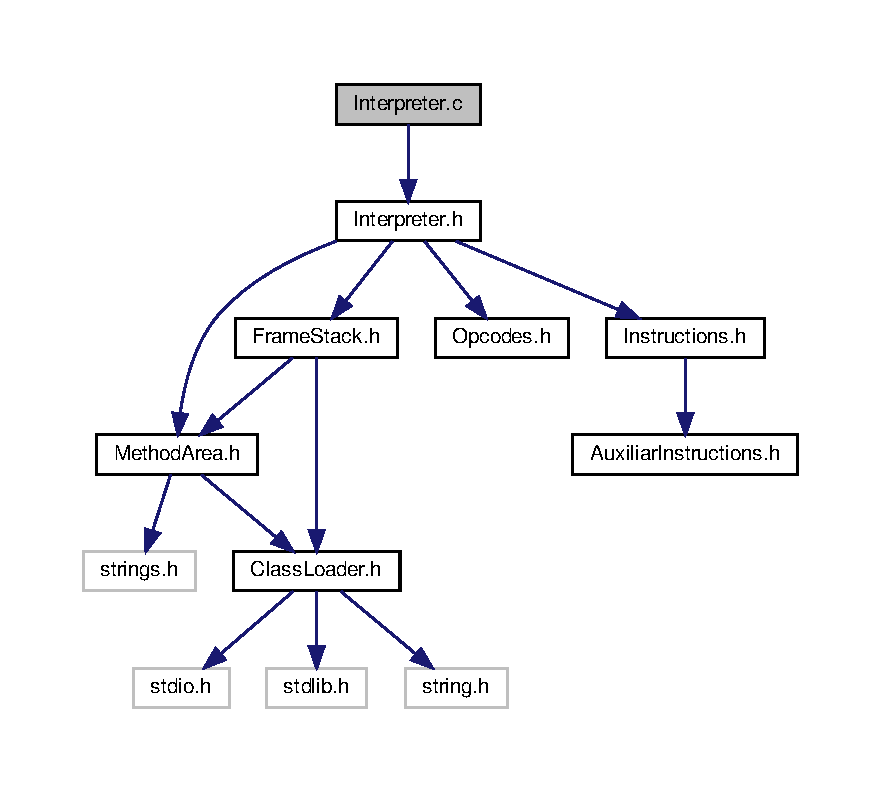
\includegraphics[width=350pt]{Interpreter_8c__incl}
\end{center}
\end{figure}
\subsection*{Funções}
\begin{DoxyCompactItemize}
\item 
void \hyperlink{Interpreter_8c_a48a27c2e0c2dd299a72e5be9427c5a0a}{executar\+Instrucao} (unsigned char \hyperlink{Opcodes_8h_a299fc707c775371e0b2b0495ccb6158e}{opcode}, \hyperlink{structFrameStack}{Frame\+Stack} $\ast$fr)
\end{DoxyCompactItemize}


\subsection{Funções}
\mbox{\Hypertarget{Interpreter_8c_a48a27c2e0c2dd299a72e5be9427c5a0a}\label{Interpreter_8c_a48a27c2e0c2dd299a72e5be9427c5a0a}} 
\index{Interpreter.\+c@{Interpreter.\+c}!executar\+Instrucao@{executar\+Instrucao}}
\index{executar\+Instrucao@{executar\+Instrucao}!Interpreter.\+c@{Interpreter.\+c}}
\subsubsection{\texorpdfstring{executar\+Instrucao()}{executarInstrucao()}}
{\footnotesize\ttfamily void executar\+Instrucao (\begin{DoxyParamCaption}\item[{unsigned char}]{opcode,  }\item[{\hyperlink{structFrameStack}{Frame\+Stack} $\ast$}]{fr }\end{DoxyParamCaption})}


\hypertarget{Interpreter_8h}{}\section{Referência do Arquivo Interpreter.\+h}
\label{Interpreter_8h}\index{Interpreter.\+h@{Interpreter.\+h}}
{\ttfamily \#include \char`\"{}Method\+Area.\+h\char`\"{}}\newline
{\ttfamily \#include \char`\"{}Frame\+Stack.\+h\char`\"{}}\newline
{\ttfamily \#include \char`\"{}Opcodes.\+h\char`\"{}}\newline
{\ttfamily \#include \char`\"{}Instructions.\+h\char`\"{}}\newline
Gráfico de dependência de inclusões para Interpreter.\+h\+:\nopagebreak
\begin{figure}[H]
\begin{center}
\leavevmode
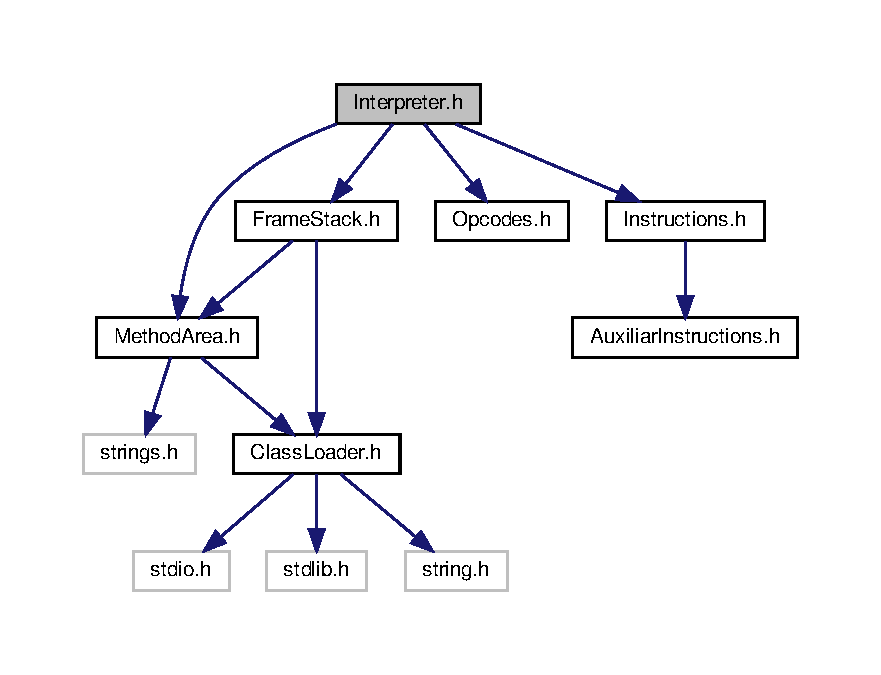
\includegraphics[width=350pt]{Interpreter_8h__incl}
\end{center}
\end{figure}
Este grafo mostra quais arquivos estão direta ou indiretamente relacionados com este arquivo\+:\nopagebreak
\begin{figure}[H]
\begin{center}
\leavevmode
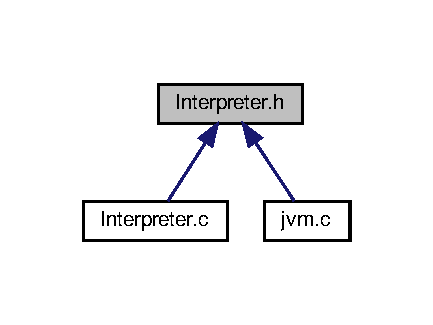
\includegraphics[width=208pt]{Interpreter_8h__dep__incl}
\end{center}
\end{figure}
\subsection*{Funções}
\begin{DoxyCompactItemize}
\item 
void \hyperlink{Interpreter_8h_afe8264d3d4324533907e8018e7d7a185}{executar} (char $\ast$method, char $\ast$descriptor, char $\ast$class\+\_\+name, int nargs, \hyperlink{structFrameStack}{Frame\+Stack} $\ast$fr, int especial)
\item 
int \hyperlink{Interpreter_8h_a2ddcc1c187ddc987628d0ab578b9bdaf}{Nargs} (char $\ast$descriptor, int length)
\item 
void \hyperlink{Interpreter_8h_a34beb517dee3ac718322e49051319d9c}{executar\+Println} (\hyperlink{structFrameStack}{Frame\+Stack} $\ast$fr, char $\ast$descriptor, int length)
\item 
void \hyperlink{Interpreter_8h_a48a27c2e0c2dd299a72e5be9427c5a0a}{executar\+Instrucao} (unsigned char \hyperlink{Opcodes_8h_a299fc707c775371e0b2b0495ccb6158e}{opcode}, \hyperlink{structFrameStack}{Frame\+Stack} $\ast$fr)
\item 
void \hyperlink{Interpreter_8h_ac43e303b11535d016ead0d667ec059dc}{executar\+Clinit} (\hyperlink{structFrameStack}{Frame\+Stack} $\ast$fr)
\end{DoxyCompactItemize}


\subsection{Funções}
\mbox{\Hypertarget{Interpreter_8h_afe8264d3d4324533907e8018e7d7a185}\label{Interpreter_8h_afe8264d3d4324533907e8018e7d7a185}} 
\index{Interpreter.\+h@{Interpreter.\+h}!executar@{executar}}
\index{executar@{executar}!Interpreter.\+h@{Interpreter.\+h}}
\subsubsection{\texorpdfstring{executar()}{executar()}}
{\footnotesize\ttfamily void executar (\begin{DoxyParamCaption}\item[{char $\ast$}]{method,  }\item[{char $\ast$}]{descriptor,  }\item[{char $\ast$}]{class\+\_\+name,  }\item[{int}]{nargs,  }\item[{\hyperlink{structFrameStack}{Frame\+Stack} $\ast$}]{fr,  }\item[{int}]{especial }\end{DoxyParamCaption})}

\mbox{\Hypertarget{Interpreter_8h_ac43e303b11535d016ead0d667ec059dc}\label{Interpreter_8h_ac43e303b11535d016ead0d667ec059dc}} 
\index{Interpreter.\+h@{Interpreter.\+h}!executar\+Clinit@{executar\+Clinit}}
\index{executar\+Clinit@{executar\+Clinit}!Interpreter.\+h@{Interpreter.\+h}}
\subsubsection{\texorpdfstring{executar\+Clinit()}{executarClinit()}}
{\footnotesize\ttfamily void executar\+Clinit (\begin{DoxyParamCaption}\item[{\hyperlink{structFrameStack}{Frame\+Stack} $\ast$}]{fr }\end{DoxyParamCaption})}

\mbox{\Hypertarget{Interpreter_8h_a48a27c2e0c2dd299a72e5be9427c5a0a}\label{Interpreter_8h_a48a27c2e0c2dd299a72e5be9427c5a0a}} 
\index{Interpreter.\+h@{Interpreter.\+h}!executar\+Instrucao@{executar\+Instrucao}}
\index{executar\+Instrucao@{executar\+Instrucao}!Interpreter.\+h@{Interpreter.\+h}}
\subsubsection{\texorpdfstring{executar\+Instrucao()}{executarInstrucao()}}
{\footnotesize\ttfamily void executar\+Instrucao (\begin{DoxyParamCaption}\item[{unsigned char}]{opcode,  }\item[{\hyperlink{structFrameStack}{Frame\+Stack} $\ast$}]{fr }\end{DoxyParamCaption})}

\mbox{\Hypertarget{Interpreter_8h_a34beb517dee3ac718322e49051319d9c}\label{Interpreter_8h_a34beb517dee3ac718322e49051319d9c}} 
\index{Interpreter.\+h@{Interpreter.\+h}!executar\+Println@{executar\+Println}}
\index{executar\+Println@{executar\+Println}!Interpreter.\+h@{Interpreter.\+h}}
\subsubsection{\texorpdfstring{executar\+Println()}{executarPrintln()}}
{\footnotesize\ttfamily void executar\+Println (\begin{DoxyParamCaption}\item[{\hyperlink{structFrameStack}{Frame\+Stack} $\ast$}]{fr,  }\item[{char $\ast$}]{descriptor,  }\item[{int}]{length }\end{DoxyParamCaption})}

\mbox{\Hypertarget{Interpreter_8h_a2ddcc1c187ddc987628d0ab578b9bdaf}\label{Interpreter_8h_a2ddcc1c187ddc987628d0ab578b9bdaf}} 
\index{Interpreter.\+h@{Interpreter.\+h}!Nargs@{Nargs}}
\index{Nargs@{Nargs}!Interpreter.\+h@{Interpreter.\+h}}
\subsubsection{\texorpdfstring{Nargs()}{Nargs()}}
{\footnotesize\ttfamily int Nargs (\begin{DoxyParamCaption}\item[{char $\ast$}]{descriptor,  }\item[{int}]{length }\end{DoxyParamCaption})}


\hypertarget{jvm_8c}{}\section{Referência do Arquivo jvm.\+c}
\label{jvm_8c}\index{jvm.\+c@{jvm.\+c}}
{\ttfamily \#include $<$stdio.\+h$>$}\newline
{\ttfamily \#include $<$string.\+h$>$}\newline
{\ttfamily \#include \char`\"{}Interpreter.\+h\char`\"{}}\newline
{\ttfamily \#include \char`\"{}exibidor.\+h\char`\"{}}\newline
Gráfico de dependência de inclusões para jvm.\+c\+:
\nopagebreak
\begin{figure}[H]
\begin{center}
\leavevmode
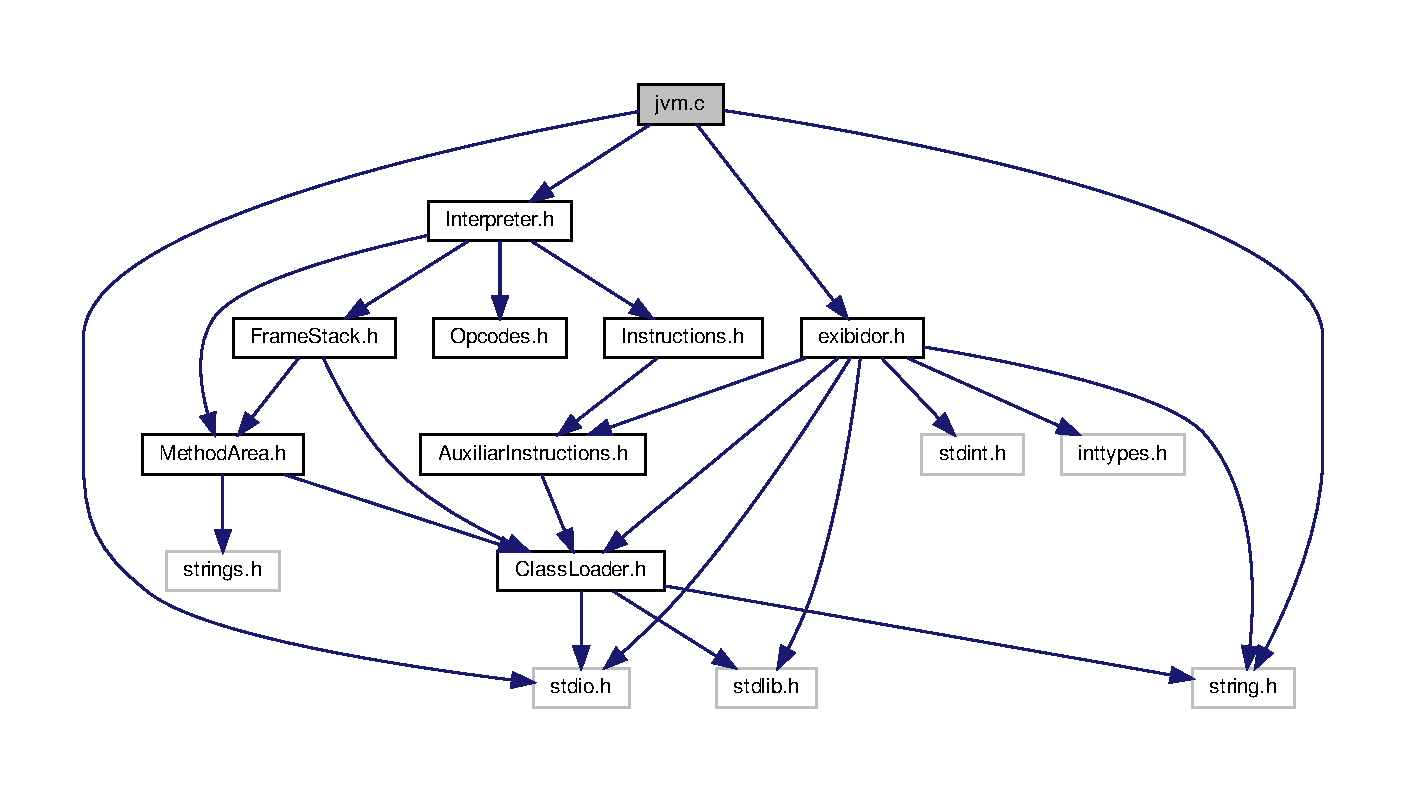
\includegraphics[width=350pt]{jvm_8c__incl}
\end{center}
\end{figure}
\subsection*{Funções}
\begin{DoxyCompactItemize}
\item 
int \hyperlink{jvm_8c_a2ddcc1c187ddc987628d0ab578b9bdaf}{Nargs} (char $\ast$descriptor, int length)
\item 
void \hyperlink{jvm_8c_a34beb517dee3ac718322e49051319d9c}{executar\+Println} (\hyperlink{structFrameStack}{Frame\+Stack} $\ast$fr, char $\ast$descriptor, int length)
\item 
void \hyperlink{jvm_8c_ac43e303b11535d016ead0d667ec059dc}{executar\+Clinit} (\hyperlink{structFrameStack}{Frame\+Stack} $\ast$fr)
\item 
void \hyperlink{jvm_8c_afe8264d3d4324533907e8018e7d7a185}{executar} (char $\ast$method, char $\ast$descriptor, char $\ast$class\+\_\+name, int nargs, \hyperlink{structFrameStack}{Frame\+Stack} $\ast$fr, int especial)
\item 
int \hyperlink{jvm_8c_a0ddf1224851353fc92bfbff6f499fa97}{main} (int argc, char $\ast$argv\mbox{[}$\,$\mbox{]})
\end{DoxyCompactItemize}


\subsection{Funções}
\mbox{\Hypertarget{jvm_8c_afe8264d3d4324533907e8018e7d7a185}\label{jvm_8c_afe8264d3d4324533907e8018e7d7a185}} 
\index{jvm.\+c@{jvm.\+c}!executar@{executar}}
\index{executar@{executar}!jvm.\+c@{jvm.\+c}}
\subsubsection{\texorpdfstring{executar()}{executar()}}
{\footnotesize\ttfamily void executar (\begin{DoxyParamCaption}\item[{char $\ast$}]{method,  }\item[{char $\ast$}]{descriptor,  }\item[{char $\ast$}]{class\+\_\+name,  }\item[{int}]{nargs,  }\item[{\hyperlink{structFrameStack}{Frame\+Stack} $\ast$}]{fr,  }\item[{int}]{especial }\end{DoxyParamCaption})}

\mbox{\Hypertarget{jvm_8c_ac43e303b11535d016ead0d667ec059dc}\label{jvm_8c_ac43e303b11535d016ead0d667ec059dc}} 
\index{jvm.\+c@{jvm.\+c}!executar\+Clinit@{executar\+Clinit}}
\index{executar\+Clinit@{executar\+Clinit}!jvm.\+c@{jvm.\+c}}
\subsubsection{\texorpdfstring{executar\+Clinit()}{executarClinit()}}
{\footnotesize\ttfamily void executar\+Clinit (\begin{DoxyParamCaption}\item[{\hyperlink{structFrameStack}{Frame\+Stack} $\ast$}]{fr }\end{DoxyParamCaption})}

\mbox{\Hypertarget{jvm_8c_a34beb517dee3ac718322e49051319d9c}\label{jvm_8c_a34beb517dee3ac718322e49051319d9c}} 
\index{jvm.\+c@{jvm.\+c}!executar\+Println@{executar\+Println}}
\index{executar\+Println@{executar\+Println}!jvm.\+c@{jvm.\+c}}
\subsubsection{\texorpdfstring{executar\+Println()}{executarPrintln()}}
{\footnotesize\ttfamily void executar\+Println (\begin{DoxyParamCaption}\item[{\hyperlink{structFrameStack}{Frame\+Stack} $\ast$}]{fr,  }\item[{char $\ast$}]{descriptor,  }\item[{int}]{length }\end{DoxyParamCaption})}

\mbox{\Hypertarget{jvm_8c_a0ddf1224851353fc92bfbff6f499fa97}\label{jvm_8c_a0ddf1224851353fc92bfbff6f499fa97}} 
\index{jvm.\+c@{jvm.\+c}!main@{main}}
\index{main@{main}!jvm.\+c@{jvm.\+c}}
\subsubsection{\texorpdfstring{main()}{main()}}
{\footnotesize\ttfamily int main (\begin{DoxyParamCaption}\item[{int}]{argc,  }\item[{char $\ast$}]{argv\mbox{[}$\,$\mbox{]} }\end{DoxyParamCaption})}

\mbox{\Hypertarget{jvm_8c_a2ddcc1c187ddc987628d0ab578b9bdaf}\label{jvm_8c_a2ddcc1c187ddc987628d0ab578b9bdaf}} 
\index{jvm.\+c@{jvm.\+c}!Nargs@{Nargs}}
\index{Nargs@{Nargs}!jvm.\+c@{jvm.\+c}}
\subsubsection{\texorpdfstring{Nargs()}{Nargs()}}
{\footnotesize\ttfamily int Nargs (\begin{DoxyParamCaption}\item[{char $\ast$}]{descriptor,  }\item[{int}]{length }\end{DoxyParamCaption})}


\hypertarget{MethodArea_8c}{}\section{Referência do Arquivo Method\+Area.\+c}
\label{MethodArea_8c}\index{Method\+Area.\+c@{Method\+Area.\+c}}
{\ttfamily \#include \char`\"{}Method\+Area.\+h\char`\"{}}\newline
Gráfico de dependência de inclusões para Method\+Area.\+c\+:\nopagebreak
\begin{figure}[H]
\begin{center}
\leavevmode
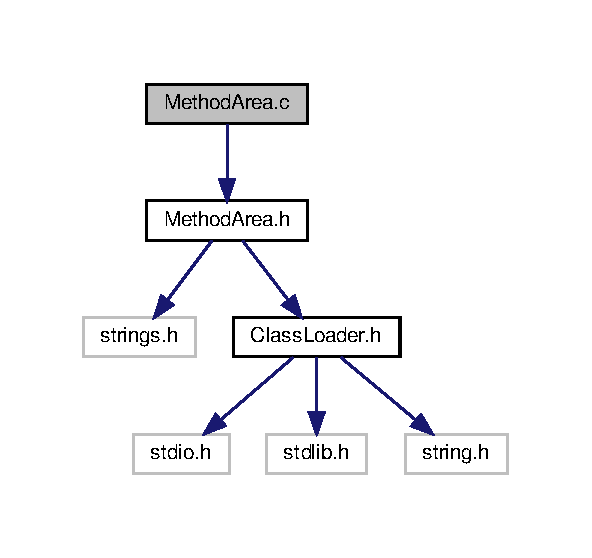
\includegraphics[width=284pt]{MethodArea_8c__incl}
\end{center}
\end{figure}
\subsection*{Funções}
\begin{DoxyCompactItemize}
\item 
void \hyperlink{MethodArea_8c_ac4fbac94288cf0cd229e1fd09183b2f5}{insert\+Class} (\hyperlink{structClass}{Class} $\ast$new\+Class)
\begin{DoxyCompactList}\small\item\em Função que insere uma classe na lista de classes. \end{DoxyCompactList}\item 
void \hyperlink{MethodArea_8c_ab63ab145475573765f2ba8751e7debbb}{destroy\+Class\+List} ()
\begin{DoxyCompactList}\small\item\em Limpa da memória toda a lista de classes. \end{DoxyCompactList}\item 
\hyperlink{structClass}{Class} $\ast$ \hyperlink{MethodArea_8c_a3c73bbfba081261f068c03a5993eaa5f}{search\+Class} (char $\ast$class\+Name)
\begin{DoxyCompactList}\small\item\em Função que procura e carrega uma classe do HD. \end{DoxyCompactList}\item 
\hyperlink{structcp__info}{cp\+\_\+info} $\ast$ \hyperlink{MethodArea_8c_af296db4d6c3b98842c7850fd72a80883}{cp\+Search} (char $\ast$class\+Name)
\begin{DoxyCompactList}\small\item\em Função que procura o constant pool. \end{DoxyCompactList}\item 
int \hyperlink{MethodArea_8c_a562ab8bca97550f9ea25092bb5e81b25}{Count\+Static\+Atrib} (\hyperlink{structClassFile}{Class\+File} $\ast$pt\+Class)
\begin{DoxyCompactList}\small\item\em Função que conta o número de atributos estáticos. \end{DoxyCompactList}\item 
int \hyperlink{MethodArea_8c_a07f2ba10edcf4fa9e42f29c1b77e25d9}{Count\+Atrib} (\hyperlink{structClassFile}{Class\+File} $\ast$pt\+Class)
\begin{DoxyCompactList}\small\item\em Função que conta o número de atributos dinâmicos. \end{DoxyCompactList}\item 
int \hyperlink{MethodArea_8c_aa543f19f820dc4c6700166fd4fb80a6a}{Type\+Descriptor} (char $\ast$descriptor)
\begin{DoxyCompactList}\small\item\em Função que procura o tipo do descritor. \end{DoxyCompactList}\item 
\hyperlink{structStaticAtrib}{Static\+Atrib} $\ast$ \hyperlink{MethodArea_8c_af6fe11c8391105d4fbeb194a5e1aa234}{static\+Load} (\hyperlink{structClassFile}{Class\+File} $\ast$cf)
\begin{DoxyCompactList}\small\item\em Função que extrai todos os parametros estáticos. \end{DoxyCompactList}\item 
\hyperlink{structObject}{Object} $\ast$ \hyperlink{MethodArea_8c_a013df09207698346ad966d4b80035bce}{create\+Object} (\hyperlink{structClassFile}{Class\+File} $\ast$cf)
\begin{DoxyCompactList}\small\item\em Função que cria um objeto. \end{DoxyCompactList}\item 
\hyperlink{structmethod__info}{method\+\_\+info} $\ast$ \hyperlink{MethodArea_8c_a998584cc00a46f1674dc97c91e1786e7}{get\+Method} (char $\ast$name, char $\ast$class\+\_\+name, char $\ast$descriptor)
\begin{DoxyCompactList}\small\item\em Função que extrai as informações de um dado método. \end{DoxyCompactList}\item 
\hyperlink{structcp__info}{cp\+\_\+info} $\ast$ \hyperlink{MethodArea_8c_a8141c4149f381e339859a57b0e2f5e68}{get\+Cp\+Super} (char $\ast$name, char $\ast$class\+\_\+name, char $\ast$descriptor)
\begin{DoxyCompactList}\small\item\em Função que procura um constant pool de um função. \end{DoxyCompactList}\item 
\hyperlink{structStaticAtrib}{Static\+Atrib} $\ast$ \hyperlink{MethodArea_8c_a6a9afe10625c496a7e6b9329feeb3874}{getstatic\+Atrib} (char $\ast$class\+\_\+name)
\begin{DoxyCompactList}\small\item\em Função que busca o vetor de variáveis estáticas. \end{DoxyCompactList}\item 
long \hyperlink{MethodArea_8c_a6c1d849ab049d6d42552889dfea989d5}{get\+N\+Atrib\+Static} (char $\ast$class\+\_\+name)
\begin{DoxyCompactList}\small\item\em Função que conta o número de atributos estáticos. \end{DoxyCompactList}\end{DoxyCompactItemize}
\subsection*{Variáveis}
\begin{DoxyCompactItemize}
\item 
\hyperlink{structClass}{Class} $\ast$ \hyperlink{MethodArea_8c_ab10f9eb1f39a25ecca6fe345f4bff710}{list} = N\+U\+LL
\end{DoxyCompactItemize}


\subsection{Funções}
\mbox{\Hypertarget{MethodArea_8c_a07f2ba10edcf4fa9e42f29c1b77e25d9}\label{MethodArea_8c_a07f2ba10edcf4fa9e42f29c1b77e25d9}} 
\index{Method\+Area.\+c@{Method\+Area.\+c}!Count\+Atrib@{Count\+Atrib}}
\index{Count\+Atrib@{Count\+Atrib}!Method\+Area.\+c@{Method\+Area.\+c}}
\subsubsection{\texorpdfstring{Count\+Atrib()}{CountAtrib()}}
{\footnotesize\ttfamily int Count\+Atrib (\begin{DoxyParamCaption}\item[{\hyperlink{structClassFile}{Class\+File} $\ast$}]{pt\+Class }\end{DoxyParamCaption})}



Função que conta o número de atributos dinâmicos. 


\begin{DoxyParams}{Parâmetros}
{\em $\ast$pt\+Class} & ponteiro para a classe \\
\hline
\end{DoxyParams}
\begin{DoxyReturn}{Retorna}
Número de atributos dinâmicos 
\end{DoxyReturn}
\mbox{\Hypertarget{MethodArea_8c_a562ab8bca97550f9ea25092bb5e81b25}\label{MethodArea_8c_a562ab8bca97550f9ea25092bb5e81b25}} 
\index{Method\+Area.\+c@{Method\+Area.\+c}!Count\+Static\+Atrib@{Count\+Static\+Atrib}}
\index{Count\+Static\+Atrib@{Count\+Static\+Atrib}!Method\+Area.\+c@{Method\+Area.\+c}}
\subsubsection{\texorpdfstring{Count\+Static\+Atrib()}{CountStaticAtrib()}}
{\footnotesize\ttfamily int Count\+Static\+Atrib (\begin{DoxyParamCaption}\item[{\hyperlink{structClassFile}{Class\+File} $\ast$}]{pt\+Class }\end{DoxyParamCaption})}



Função que conta o número de atributos estáticos. 


\begin{DoxyParams}{Parâmetros}
{\em $\ast$pt\+Class} & ponteiro para a classe \\
\hline
\end{DoxyParams}
\begin{DoxyReturn}{Retorna}
Número de atributos estáticos 
\end{DoxyReturn}
\mbox{\Hypertarget{MethodArea_8c_af296db4d6c3b98842c7850fd72a80883}\label{MethodArea_8c_af296db4d6c3b98842c7850fd72a80883}} 
\index{Method\+Area.\+c@{Method\+Area.\+c}!cp\+Search@{cp\+Search}}
\index{cp\+Search@{cp\+Search}!Method\+Area.\+c@{Method\+Area.\+c}}
\subsubsection{\texorpdfstring{cp\+Search()}{cpSearch()}}
{\footnotesize\ttfamily \hyperlink{structcp__info}{cp\+\_\+info}$\ast$ cp\+Search (\begin{DoxyParamCaption}\item[{char $\ast$}]{class\+Name }\end{DoxyParamCaption})}



Função que procura o constant pool. 


\begin{DoxyParams}{Parâmetros}
{\em $\ast$class\+Name} & Nome da classe \\
\hline
\end{DoxyParams}
\begin{DoxyReturn}{Retorna}
Ponteiro para o constant poll 
\end{DoxyReturn}
\mbox{\Hypertarget{MethodArea_8c_a013df09207698346ad966d4b80035bce}\label{MethodArea_8c_a013df09207698346ad966d4b80035bce}} 
\index{Method\+Area.\+c@{Method\+Area.\+c}!create\+Object@{create\+Object}}
\index{create\+Object@{create\+Object}!Method\+Area.\+c@{Method\+Area.\+c}}
\subsubsection{\texorpdfstring{create\+Object()}{createObject()}}
{\footnotesize\ttfamily \hyperlink{structObject}{Object}$\ast$ create\+Object (\begin{DoxyParamCaption}\item[{\hyperlink{structClassFile}{Class\+File} $\ast$}]{cf }\end{DoxyParamCaption})}



Função que cria um objeto. 


\begin{DoxyParams}{Parâmetros}
{\em $\ast$cf} & Ponteiro para a classe \\
\hline
\end{DoxyParams}
\begin{DoxyReturn}{Retorna}
Ponteiro para o objeto 
\end{DoxyReturn}
\mbox{\Hypertarget{MethodArea_8c_ab63ab145475573765f2ba8751e7debbb}\label{MethodArea_8c_ab63ab145475573765f2ba8751e7debbb}} 
\index{Method\+Area.\+c@{Method\+Area.\+c}!destroy\+Class\+List@{destroy\+Class\+List}}
\index{destroy\+Class\+List@{destroy\+Class\+List}!Method\+Area.\+c@{Method\+Area.\+c}}
\subsubsection{\texorpdfstring{destroy\+Class\+List()}{destroyClassList()}}
{\footnotesize\ttfamily void destroy\+Class\+List (\begin{DoxyParamCaption}{ }\end{DoxyParamCaption})}



Limpa da memória toda a lista de classes. 

\mbox{\Hypertarget{MethodArea_8c_a8141c4149f381e339859a57b0e2f5e68}\label{MethodArea_8c_a8141c4149f381e339859a57b0e2f5e68}} 
\index{Method\+Area.\+c@{Method\+Area.\+c}!get\+Cp\+Super@{get\+Cp\+Super}}
\index{get\+Cp\+Super@{get\+Cp\+Super}!Method\+Area.\+c@{Method\+Area.\+c}}
\subsubsection{\texorpdfstring{get\+Cp\+Super()}{getCpSuper()}}
{\footnotesize\ttfamily \hyperlink{structcp__info}{cp\+\_\+info}$\ast$ get\+Cp\+Super (\begin{DoxyParamCaption}\item[{char $\ast$}]{name,  }\item[{char $\ast$}]{class\+\_\+name,  }\item[{char $\ast$}]{descriptor }\end{DoxyParamCaption})}



Função que procura um constant pool de um função. 


\begin{DoxyParams}{Parâmetros}
{\em $\ast$name} & Nome do método \\
\hline
{\em $\ast$class\+\_\+name} & Nome da classe que contém esse método \\
\hline
{\em $\ast$descritor} & Descritor do método \\
\hline
\end{DoxyParams}
\begin{DoxyReturn}{Retorna}
Ponteiro para o constant pool 
\end{DoxyReturn}
\mbox{\Hypertarget{MethodArea_8c_a998584cc00a46f1674dc97c91e1786e7}\label{MethodArea_8c_a998584cc00a46f1674dc97c91e1786e7}} 
\index{Method\+Area.\+c@{Method\+Area.\+c}!get\+Method@{get\+Method}}
\index{get\+Method@{get\+Method}!Method\+Area.\+c@{Method\+Area.\+c}}
\subsubsection{\texorpdfstring{get\+Method()}{getMethod()}}
{\footnotesize\ttfamily \hyperlink{structmethod__info}{method\+\_\+info}$\ast$ get\+Method (\begin{DoxyParamCaption}\item[{char $\ast$}]{name,  }\item[{char $\ast$}]{class\+\_\+name,  }\item[{char $\ast$}]{descriptor }\end{DoxyParamCaption})}



Função que extrai as informações de um dado método. 


\begin{DoxyParams}{Parâmetros}
{\em $\ast$name} & Nome do método \\
\hline
{\em $\ast$class\+\_\+name} & Nome da classe que contém esse método \\
\hline
{\em $\ast$descritor} & Descritor do método \\
\hline
\end{DoxyParams}
\begin{DoxyReturn}{Retorna}
Ponteiro para a estrutura que guarda as informações do método 
\end{DoxyReturn}
\mbox{\Hypertarget{MethodArea_8c_a6c1d849ab049d6d42552889dfea989d5}\label{MethodArea_8c_a6c1d849ab049d6d42552889dfea989d5}} 
\index{Method\+Area.\+c@{Method\+Area.\+c}!get\+N\+Atrib\+Static@{get\+N\+Atrib\+Static}}
\index{get\+N\+Atrib\+Static@{get\+N\+Atrib\+Static}!Method\+Area.\+c@{Method\+Area.\+c}}
\subsubsection{\texorpdfstring{get\+N\+Atrib\+Static()}{getNAtribStatic()}}
{\footnotesize\ttfamily long get\+N\+Atrib\+Static (\begin{DoxyParamCaption}\item[{char $\ast$}]{class\+\_\+name }\end{DoxyParamCaption})}



Função que conta o número de atributos estáticos. 


\begin{DoxyParams}{Parâmetros}
{\em $\ast$class\+\_\+name} & nome da classe \\
\hline
\end{DoxyParams}
\begin{DoxyReturn}{Retorna}
Número de atributos estáticos 
\end{DoxyReturn}
\mbox{\Hypertarget{MethodArea_8c_a6a9afe10625c496a7e6b9329feeb3874}\label{MethodArea_8c_a6a9afe10625c496a7e6b9329feeb3874}} 
\index{Method\+Area.\+c@{Method\+Area.\+c}!getstatic\+Atrib@{getstatic\+Atrib}}
\index{getstatic\+Atrib@{getstatic\+Atrib}!Method\+Area.\+c@{Method\+Area.\+c}}
\subsubsection{\texorpdfstring{getstatic\+Atrib()}{getstaticAtrib()}}
{\footnotesize\ttfamily \hyperlink{structStaticAtrib}{Static\+Atrib}$\ast$ getstatic\+Atrib (\begin{DoxyParamCaption}\item[{char $\ast$}]{class\+\_\+name }\end{DoxyParamCaption})}



Função que busca o vetor de variáveis estáticas. 


\begin{DoxyParams}{Parâmetros}
{\em $\ast$class\+\_\+name} & nome da classe \\
\hline
\end{DoxyParams}
\begin{DoxyReturn}{Retorna}
Ponteiro para o vetor de variáveis estáticas 
\end{DoxyReturn}
\mbox{\Hypertarget{MethodArea_8c_ac4fbac94288cf0cd229e1fd09183b2f5}\label{MethodArea_8c_ac4fbac94288cf0cd229e1fd09183b2f5}} 
\index{Method\+Area.\+c@{Method\+Area.\+c}!insert\+Class@{insert\+Class}}
\index{insert\+Class@{insert\+Class}!Method\+Area.\+c@{Method\+Area.\+c}}
\subsubsection{\texorpdfstring{insert\+Class()}{insertClass()}}
{\footnotesize\ttfamily void insert\+Class (\begin{DoxyParamCaption}\item[{\hyperlink{structClass}{Class} $\ast$}]{new\+Class }\end{DoxyParamCaption})}



Função que insere uma classe na lista de classes. 


\begin{DoxyParams}{Parâmetros}
{\em $\ast$new\+Class} & Ponteiro para a classe a ser inserida \\
\hline
\end{DoxyParams}
\mbox{\Hypertarget{MethodArea_8c_a3c73bbfba081261f068c03a5993eaa5f}\label{MethodArea_8c_a3c73bbfba081261f068c03a5993eaa5f}} 
\index{Method\+Area.\+c@{Method\+Area.\+c}!search\+Class@{search\+Class}}
\index{search\+Class@{search\+Class}!Method\+Area.\+c@{Method\+Area.\+c}}
\subsubsection{\texorpdfstring{search\+Class()}{searchClass()}}
{\footnotesize\ttfamily \hyperlink{structClass}{Class}$\ast$ search\+Class (\begin{DoxyParamCaption}\item[{char $\ast$}]{class\+Name }\end{DoxyParamCaption})}



Função que procura e carrega uma classe do HD. 


\begin{DoxyParams}{Parâmetros}
{\em $\ast$class\+Name} & Endereço da classe \\
\hline
\end{DoxyParams}
\begin{DoxyReturn}{Retorna}
Ponteiro para a classe 
\end{DoxyReturn}
\mbox{\Hypertarget{MethodArea_8c_af6fe11c8391105d4fbeb194a5e1aa234}\label{MethodArea_8c_af6fe11c8391105d4fbeb194a5e1aa234}} 
\index{Method\+Area.\+c@{Method\+Area.\+c}!static\+Load@{static\+Load}}
\index{static\+Load@{static\+Load}!Method\+Area.\+c@{Method\+Area.\+c}}
\subsubsection{\texorpdfstring{static\+Load()}{staticLoad()}}
{\footnotesize\ttfamily \hyperlink{structStaticAtrib}{Static\+Atrib}$\ast$ static\+Load (\begin{DoxyParamCaption}\item[{\hyperlink{structClassFile}{Class\+File} $\ast$}]{cf }\end{DoxyParamCaption})}



Função que extrai todos os parametros estáticos. 


\begin{DoxyParams}{Parâmetros}
{\em $\ast$cf} & Ponteiro para a classe \\
\hline
\end{DoxyParams}
\begin{DoxyReturn}{Retorna}
Vetor de variáveis estáticas 
\end{DoxyReturn}
\mbox{\Hypertarget{MethodArea_8c_aa543f19f820dc4c6700166fd4fb80a6a}\label{MethodArea_8c_aa543f19f820dc4c6700166fd4fb80a6a}} 
\index{Method\+Area.\+c@{Method\+Area.\+c}!Type\+Descriptor@{Type\+Descriptor}}
\index{Type\+Descriptor@{Type\+Descriptor}!Method\+Area.\+c@{Method\+Area.\+c}}
\subsubsection{\texorpdfstring{Type\+Descriptor()}{TypeDescriptor()}}
{\footnotesize\ttfamily int Type\+Descriptor (\begin{DoxyParamCaption}\item[{char $\ast$}]{descriptor }\end{DoxyParamCaption})}



Função que procura o tipo do descritor. 


\begin{DoxyParams}{Parâmetros}
{\em $\ast$descritor} & string do descritor \\
\hline
\end{DoxyParams}
\begin{DoxyReturn}{Retorna}
Número referente a esse descritor 
\end{DoxyReturn}


\subsection{Variáveis}
\mbox{\Hypertarget{MethodArea_8c_ab10f9eb1f39a25ecca6fe345f4bff710}\label{MethodArea_8c_ab10f9eb1f39a25ecca6fe345f4bff710}} 
\index{Method\+Area.\+c@{Method\+Area.\+c}!list@{list}}
\index{list@{list}!Method\+Area.\+c@{Method\+Area.\+c}}
\subsubsection{\texorpdfstring{list}{list}}
{\footnotesize\ttfamily \hyperlink{structClass}{Class}$\ast$ list = N\+U\+LL}


\hypertarget{MethodArea_8h}{}\section{Referência do Arquivo Method\+Area.\+h}
\label{MethodArea_8h}\index{Method\+Area.\+h@{Method\+Area.\+h}}
{\ttfamily \#include $<$strings.\+h$>$}\newline
{\ttfamily \#include \char`\"{}Class\+Loader.\+h\char`\"{}}\newline
Gráfico de dependência de inclusões para Method\+Area.\+h\+:\nopagebreak
\begin{figure}[H]
\begin{center}
\leavevmode
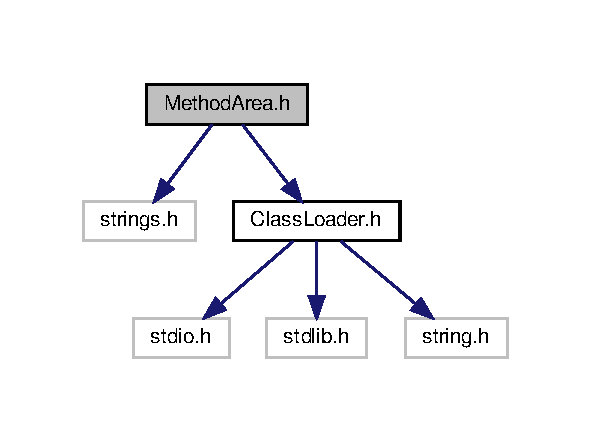
\includegraphics[width=284pt]{MethodArea_8h__incl}
\end{center}
\end{figure}
Este grafo mostra quais arquivos estão direta ou indiretamente relacionados com este arquivo\+:\nopagebreak
\begin{figure}[H]
\begin{center}
\leavevmode
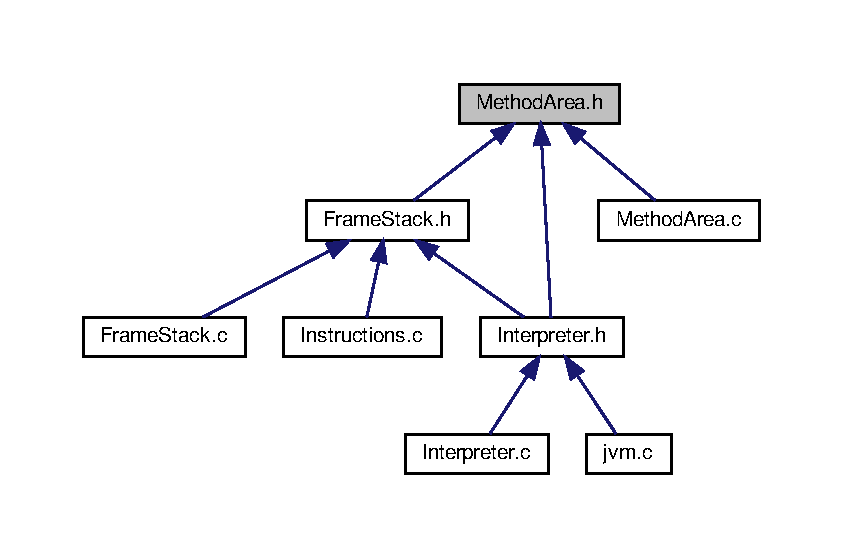
\includegraphics[width=350pt]{MethodArea_8h__dep__incl}
\end{center}
\end{figure}
\subsection*{Componentes}
\begin{DoxyCompactItemize}
\item 
struct \hyperlink{structarrayMult}{array\+Mult}
\begin{DoxyCompactList}\small\item\em Estrutura que gerencia os array multidimensionais. \end{DoxyCompactList}\item 
union \hyperlink{unionDataStaticAtrib}{Data\+Static\+Atrib}
\begin{DoxyCompactList}\small\item\em Estrutura que gerencia os atributos estáticos para cada tipo. \end{DoxyCompactList}\item 
struct \hyperlink{structStaticAtrib}{Static\+Atrib}
\begin{DoxyCompactList}\small\item\em Estrutura que gerencia os atributos estáticos, mais geral. \end{DoxyCompactList}\item 
union \hyperlink{unionDataAtrib}{Data\+Atrib}
\begin{DoxyCompactList}\small\item\em Estrutura que gerencia os atributos dinâmicos para cada tipo. \end{DoxyCompactList}\item 
struct \hyperlink{structObject}{Object}
\begin{DoxyCompactList}\small\item\em Estrutura que gerencia os atributos dinâmicos, mais geral. \end{DoxyCompactList}\item 
struct \hyperlink{structClass}{Class}
\begin{DoxyCompactList}\small\item\em Estrutura que gerencia uma classe carregada. \end{DoxyCompactList}\end{DoxyCompactItemize}
\subsection*{Definições de Tipos}
\begin{DoxyCompactItemize}
\item 
typedef struct \hyperlink{structarrayMult}{array\+Mult} \hyperlink{MethodArea_8h_a7cb54570c81d925b2e5825171a73bd84}{array\+Mult}
\begin{DoxyCompactList}\small\item\em Estrutura que gerencia os array multidimensionais. \end{DoxyCompactList}\item 
typedef union \hyperlink{unionDataStaticAtrib}{Data\+Static\+Atrib} \hyperlink{MethodArea_8h_a008393c9ee4f7e420482ca040fbef5cc}{Data\+Static\+Atrib}
\begin{DoxyCompactList}\small\item\em Estrutura que gerencia os atributos estáticos para cada tipo. \end{DoxyCompactList}\item 
typedef struct \hyperlink{structStaticAtrib}{Static\+Atrib} \hyperlink{MethodArea_8h_a19a1a9a62ffeef237d0cf65a9ea929c7}{Static\+Atrib}
\begin{DoxyCompactList}\small\item\em Estrutura que gerencia os atributos estáticos, mais geral. \end{DoxyCompactList}\item 
typedef union \hyperlink{unionDataAtrib}{Data\+Atrib} \hyperlink{MethodArea_8h_adbf41dff677d2ea31074fee3016882e5}{Data\+Atrib}
\begin{DoxyCompactList}\small\item\em Estrutura que gerencia os atributos dinâmicos para cada tipo. \end{DoxyCompactList}\item 
typedef struct \hyperlink{structObject}{Object} \hyperlink{MethodArea_8h_ab1287b6141419421dc5c14b9f7756b0a}{Object}
\begin{DoxyCompactList}\small\item\em Estrutura que gerencia os atributos dinâmicos, mais geral. \end{DoxyCompactList}\item 
typedef struct \hyperlink{structClass}{Class} \hyperlink{MethodArea_8h_a9c158af314b0aa46ba0d0e19cef592d8}{Class}
\begin{DoxyCompactList}\small\item\em Estrutura que gerencia uma classe carregada. \end{DoxyCompactList}\end{DoxyCompactItemize}
\subsection*{Funções}
\begin{DoxyCompactItemize}
\item 
void \hyperlink{MethodArea_8h_ac4fbac94288cf0cd229e1fd09183b2f5}{insert\+Class} (\hyperlink{structClass}{Class} $\ast$new\+Class)
\begin{DoxyCompactList}\small\item\em Função que insere uma classe na lista de classes. \end{DoxyCompactList}\item 
void \hyperlink{MethodArea_8h_ab63ab145475573765f2ba8751e7debbb}{destroy\+Class\+List} ()
\begin{DoxyCompactList}\small\item\em Limpa da memória toda a lista de classes. \end{DoxyCompactList}\item 
\hyperlink{structStaticAtrib}{Static\+Atrib} $\ast$ \hyperlink{MethodArea_8h_af6fe11c8391105d4fbeb194a5e1aa234}{static\+Load} (\hyperlink{structClassFile}{Class\+File} $\ast$cf)
\begin{DoxyCompactList}\small\item\em Função que extrai todos os parametros estáticos. \end{DoxyCompactList}\item 
\hyperlink{structClass}{Class} $\ast$ \hyperlink{MethodArea_8h_a3c73bbfba081261f068c03a5993eaa5f}{search\+Class} (char $\ast$class\+Name)
\begin{DoxyCompactList}\small\item\em Função que procura e carrega uma classe do HD. \end{DoxyCompactList}\item 
\hyperlink{structcp__info}{cp\+\_\+info} $\ast$ \hyperlink{MethodArea_8h_af296db4d6c3b98842c7850fd72a80883}{cp\+Search} (char $\ast$class\+Name)
\begin{DoxyCompactList}\small\item\em Função que procura o constant pool. \end{DoxyCompactList}\item 
\hyperlink{structmethod__info}{method\+\_\+info} $\ast$ \hyperlink{MethodArea_8h_a998584cc00a46f1674dc97c91e1786e7}{get\+Method} (char $\ast$name, char $\ast$class\+\_\+name, char $\ast$descriptor)
\begin{DoxyCompactList}\small\item\em Função que extrai as informações de um dado método. \end{DoxyCompactList}\item 
\hyperlink{structStaticAtrib}{Static\+Atrib} $\ast$ \hyperlink{MethodArea_8h_a6a9afe10625c496a7e6b9329feeb3874}{getstatic\+Atrib} (char $\ast$class\+\_\+name)
\begin{DoxyCompactList}\small\item\em Função que busca o vetor de variáveis estáticas. \end{DoxyCompactList}\item 
long \hyperlink{MethodArea_8h_a6c1d849ab049d6d42552889dfea989d5}{get\+N\+Atrib\+Static} (char $\ast$class\+\_\+name)
\begin{DoxyCompactList}\small\item\em Função que conta o número de atributos estáticos. \end{DoxyCompactList}\item 
int \hyperlink{MethodArea_8h_a562ab8bca97550f9ea25092bb5e81b25}{Count\+Static\+Atrib} (\hyperlink{structClassFile}{Class\+File} $\ast$pt\+Class)
\begin{DoxyCompactList}\small\item\em Função que conta o número de atributos estáticos. \end{DoxyCompactList}\item 
int \hyperlink{MethodArea_8h_a07f2ba10edcf4fa9e42f29c1b77e25d9}{Count\+Atrib} (\hyperlink{structClassFile}{Class\+File} $\ast$pt\+Class)
\begin{DoxyCompactList}\small\item\em Função que conta o número de atributos dinâmicos. \end{DoxyCompactList}\item 
int \hyperlink{MethodArea_8h_aa543f19f820dc4c6700166fd4fb80a6a}{Type\+Descriptor} (char $\ast$descriptor)
\begin{DoxyCompactList}\small\item\em Função que procura o tipo do descritor. \end{DoxyCompactList}\item 
\hyperlink{structObject}{Object} $\ast$ \hyperlink{MethodArea_8h_a013df09207698346ad966d4b80035bce}{create\+Object} (\hyperlink{structClassFile}{Class\+File} $\ast$cf)
\begin{DoxyCompactList}\small\item\em Função que cria um objeto. \end{DoxyCompactList}\item 
\hyperlink{structcp__info}{cp\+\_\+info} $\ast$ \hyperlink{MethodArea_8h_a8141c4149f381e339859a57b0e2f5e68}{get\+Cp\+Super} (char $\ast$name, char $\ast$class\+\_\+name, char $\ast$descriptor)
\begin{DoxyCompactList}\small\item\em Função que procura um constant pool de um função. \end{DoxyCompactList}\end{DoxyCompactItemize}


\subsection{Definições dos tipos}
\mbox{\Hypertarget{MethodArea_8h_a7cb54570c81d925b2e5825171a73bd84}\label{MethodArea_8h_a7cb54570c81d925b2e5825171a73bd84}} 
\index{Method\+Area.\+h@{Method\+Area.\+h}!array\+Mult@{array\+Mult}}
\index{array\+Mult@{array\+Mult}!Method\+Area.\+h@{Method\+Area.\+h}}
\subsubsection{\texorpdfstring{array\+Mult}{arrayMult}}
{\footnotesize\ttfamily typedef struct \hyperlink{structarrayMult}{array\+Mult} \hyperlink{structarrayMult}{array\+Mult}}



Estrutura que gerencia os array multidimensionais. 

\mbox{\Hypertarget{MethodArea_8h_a9c158af314b0aa46ba0d0e19cef592d8}\label{MethodArea_8h_a9c158af314b0aa46ba0d0e19cef592d8}} 
\index{Method\+Area.\+h@{Method\+Area.\+h}!Class@{Class}}
\index{Class@{Class}!Method\+Area.\+h@{Method\+Area.\+h}}
\subsubsection{\texorpdfstring{Class}{Class}}
{\footnotesize\ttfamily typedef struct \hyperlink{structClass}{Class} \hyperlink{structClass}{Class}}



Estrutura que gerencia uma classe carregada. 

\mbox{\Hypertarget{MethodArea_8h_adbf41dff677d2ea31074fee3016882e5}\label{MethodArea_8h_adbf41dff677d2ea31074fee3016882e5}} 
\index{Method\+Area.\+h@{Method\+Area.\+h}!Data\+Atrib@{Data\+Atrib}}
\index{Data\+Atrib@{Data\+Atrib}!Method\+Area.\+h@{Method\+Area.\+h}}
\subsubsection{\texorpdfstring{Data\+Atrib}{DataAtrib}}
{\footnotesize\ttfamily typedef union \hyperlink{unionDataAtrib}{Data\+Atrib} \hyperlink{unionDataAtrib}{Data\+Atrib}}



Estrutura que gerencia os atributos dinâmicos para cada tipo. 

\mbox{\Hypertarget{MethodArea_8h_a008393c9ee4f7e420482ca040fbef5cc}\label{MethodArea_8h_a008393c9ee4f7e420482ca040fbef5cc}} 
\index{Method\+Area.\+h@{Method\+Area.\+h}!Data\+Static\+Atrib@{Data\+Static\+Atrib}}
\index{Data\+Static\+Atrib@{Data\+Static\+Atrib}!Method\+Area.\+h@{Method\+Area.\+h}}
\subsubsection{\texorpdfstring{Data\+Static\+Atrib}{DataStaticAtrib}}
{\footnotesize\ttfamily typedef union \hyperlink{unionDataStaticAtrib}{Data\+Static\+Atrib} \hyperlink{unionDataStaticAtrib}{Data\+Static\+Atrib}}



Estrutura que gerencia os atributos estáticos para cada tipo. 

\mbox{\Hypertarget{MethodArea_8h_ab1287b6141419421dc5c14b9f7756b0a}\label{MethodArea_8h_ab1287b6141419421dc5c14b9f7756b0a}} 
\index{Method\+Area.\+h@{Method\+Area.\+h}!Object@{Object}}
\index{Object@{Object}!Method\+Area.\+h@{Method\+Area.\+h}}
\subsubsection{\texorpdfstring{Object}{Object}}
{\footnotesize\ttfamily typedef struct \hyperlink{structObject}{Object} \hyperlink{structObject}{Object}}



Estrutura que gerencia os atributos dinâmicos, mais geral. 

\mbox{\Hypertarget{MethodArea_8h_a19a1a9a62ffeef237d0cf65a9ea929c7}\label{MethodArea_8h_a19a1a9a62ffeef237d0cf65a9ea929c7}} 
\index{Method\+Area.\+h@{Method\+Area.\+h}!Static\+Atrib@{Static\+Atrib}}
\index{Static\+Atrib@{Static\+Atrib}!Method\+Area.\+h@{Method\+Area.\+h}}
\subsubsection{\texorpdfstring{Static\+Atrib}{StaticAtrib}}
{\footnotesize\ttfamily typedef struct \hyperlink{structStaticAtrib}{Static\+Atrib} \hyperlink{structStaticAtrib}{Static\+Atrib}}



Estrutura que gerencia os atributos estáticos, mais geral. 



\subsection{Funções}
\mbox{\Hypertarget{MethodArea_8h_a07f2ba10edcf4fa9e42f29c1b77e25d9}\label{MethodArea_8h_a07f2ba10edcf4fa9e42f29c1b77e25d9}} 
\index{Method\+Area.\+h@{Method\+Area.\+h}!Count\+Atrib@{Count\+Atrib}}
\index{Count\+Atrib@{Count\+Atrib}!Method\+Area.\+h@{Method\+Area.\+h}}
\subsubsection{\texorpdfstring{Count\+Atrib()}{CountAtrib()}}
{\footnotesize\ttfamily int Count\+Atrib (\begin{DoxyParamCaption}\item[{\hyperlink{structClassFile}{Class\+File} $\ast$}]{pt\+Class }\end{DoxyParamCaption})}



Função que conta o número de atributos dinâmicos. 


\begin{DoxyParams}{Parâmetros}
{\em $\ast$pt\+Class} & ponteiro para a classe \\
\hline
\end{DoxyParams}
\begin{DoxyReturn}{Retorna}
Número de atributos dinâmicos 
\end{DoxyReturn}
\mbox{\Hypertarget{MethodArea_8h_a562ab8bca97550f9ea25092bb5e81b25}\label{MethodArea_8h_a562ab8bca97550f9ea25092bb5e81b25}} 
\index{Method\+Area.\+h@{Method\+Area.\+h}!Count\+Static\+Atrib@{Count\+Static\+Atrib}}
\index{Count\+Static\+Atrib@{Count\+Static\+Atrib}!Method\+Area.\+h@{Method\+Area.\+h}}
\subsubsection{\texorpdfstring{Count\+Static\+Atrib()}{CountStaticAtrib()}}
{\footnotesize\ttfamily int Count\+Static\+Atrib (\begin{DoxyParamCaption}\item[{\hyperlink{structClassFile}{Class\+File} $\ast$}]{pt\+Class }\end{DoxyParamCaption})}



Função que conta o número de atributos estáticos. 


\begin{DoxyParams}{Parâmetros}
{\em $\ast$pt\+Class} & ponteiro para a classe \\
\hline
\end{DoxyParams}
\begin{DoxyReturn}{Retorna}
Número de atributos estáticos 
\end{DoxyReturn}
\mbox{\Hypertarget{MethodArea_8h_af296db4d6c3b98842c7850fd72a80883}\label{MethodArea_8h_af296db4d6c3b98842c7850fd72a80883}} 
\index{Method\+Area.\+h@{Method\+Area.\+h}!cp\+Search@{cp\+Search}}
\index{cp\+Search@{cp\+Search}!Method\+Area.\+h@{Method\+Area.\+h}}
\subsubsection{\texorpdfstring{cp\+Search()}{cpSearch()}}
{\footnotesize\ttfamily \hyperlink{structcp__info}{cp\+\_\+info}$\ast$ cp\+Search (\begin{DoxyParamCaption}\item[{char $\ast$}]{class\+Name }\end{DoxyParamCaption})}



Função que procura o constant pool. 


\begin{DoxyParams}{Parâmetros}
{\em $\ast$class\+Name} & Nome da classe \\
\hline
\end{DoxyParams}
\begin{DoxyReturn}{Retorna}
Ponteiro para o constant poll 
\end{DoxyReturn}
\mbox{\Hypertarget{MethodArea_8h_a013df09207698346ad966d4b80035bce}\label{MethodArea_8h_a013df09207698346ad966d4b80035bce}} 
\index{Method\+Area.\+h@{Method\+Area.\+h}!create\+Object@{create\+Object}}
\index{create\+Object@{create\+Object}!Method\+Area.\+h@{Method\+Area.\+h}}
\subsubsection{\texorpdfstring{create\+Object()}{createObject()}}
{\footnotesize\ttfamily \hyperlink{structObject}{Object}$\ast$ create\+Object (\begin{DoxyParamCaption}\item[{\hyperlink{structClassFile}{Class\+File} $\ast$}]{cf }\end{DoxyParamCaption})}



Função que cria um objeto. 


\begin{DoxyParams}{Parâmetros}
{\em $\ast$cf} & Ponteiro para a classe \\
\hline
\end{DoxyParams}
\begin{DoxyReturn}{Retorna}
Ponteiro para o objeto 
\end{DoxyReturn}
\mbox{\Hypertarget{MethodArea_8h_ab63ab145475573765f2ba8751e7debbb}\label{MethodArea_8h_ab63ab145475573765f2ba8751e7debbb}} 
\index{Method\+Area.\+h@{Method\+Area.\+h}!destroy\+Class\+List@{destroy\+Class\+List}}
\index{destroy\+Class\+List@{destroy\+Class\+List}!Method\+Area.\+h@{Method\+Area.\+h}}
\subsubsection{\texorpdfstring{destroy\+Class\+List()}{destroyClassList()}}
{\footnotesize\ttfamily void destroy\+Class\+List (\begin{DoxyParamCaption}{ }\end{DoxyParamCaption})}



Limpa da memória toda a lista de classes. 

\mbox{\Hypertarget{MethodArea_8h_a8141c4149f381e339859a57b0e2f5e68}\label{MethodArea_8h_a8141c4149f381e339859a57b0e2f5e68}} 
\index{Method\+Area.\+h@{Method\+Area.\+h}!get\+Cp\+Super@{get\+Cp\+Super}}
\index{get\+Cp\+Super@{get\+Cp\+Super}!Method\+Area.\+h@{Method\+Area.\+h}}
\subsubsection{\texorpdfstring{get\+Cp\+Super()}{getCpSuper()}}
{\footnotesize\ttfamily \hyperlink{structcp__info}{cp\+\_\+info}$\ast$ get\+Cp\+Super (\begin{DoxyParamCaption}\item[{char $\ast$}]{name,  }\item[{char $\ast$}]{class\+\_\+name,  }\item[{char $\ast$}]{descriptor }\end{DoxyParamCaption})}



Função que procura um constant pool de um função. 


\begin{DoxyParams}{Parâmetros}
{\em $\ast$name} & Nome do método \\
\hline
{\em $\ast$class\+\_\+name} & Nome da classe que contém esse método \\
\hline
{\em $\ast$descritor} & Descritor do método \\
\hline
\end{DoxyParams}
\begin{DoxyReturn}{Retorna}
Ponteiro para o constant pool 
\end{DoxyReturn}
\mbox{\Hypertarget{MethodArea_8h_a998584cc00a46f1674dc97c91e1786e7}\label{MethodArea_8h_a998584cc00a46f1674dc97c91e1786e7}} 
\index{Method\+Area.\+h@{Method\+Area.\+h}!get\+Method@{get\+Method}}
\index{get\+Method@{get\+Method}!Method\+Area.\+h@{Method\+Area.\+h}}
\subsubsection{\texorpdfstring{get\+Method()}{getMethod()}}
{\footnotesize\ttfamily \hyperlink{structmethod__info}{method\+\_\+info}$\ast$ get\+Method (\begin{DoxyParamCaption}\item[{char $\ast$}]{name,  }\item[{char $\ast$}]{class\+\_\+name,  }\item[{char $\ast$}]{descriptor }\end{DoxyParamCaption})}



Função que extrai as informações de um dado método. 


\begin{DoxyParams}{Parâmetros}
{\em $\ast$name} & Nome do método \\
\hline
{\em $\ast$class\+\_\+name} & Nome da classe que contém esse método \\
\hline
{\em $\ast$descritor} & Descritor do método \\
\hline
\end{DoxyParams}
\begin{DoxyReturn}{Retorna}
Ponteiro para a estrutura que guarda as informações do método 
\end{DoxyReturn}
\mbox{\Hypertarget{MethodArea_8h_a6c1d849ab049d6d42552889dfea989d5}\label{MethodArea_8h_a6c1d849ab049d6d42552889dfea989d5}} 
\index{Method\+Area.\+h@{Method\+Area.\+h}!get\+N\+Atrib\+Static@{get\+N\+Atrib\+Static}}
\index{get\+N\+Atrib\+Static@{get\+N\+Atrib\+Static}!Method\+Area.\+h@{Method\+Area.\+h}}
\subsubsection{\texorpdfstring{get\+N\+Atrib\+Static()}{getNAtribStatic()}}
{\footnotesize\ttfamily long get\+N\+Atrib\+Static (\begin{DoxyParamCaption}\item[{char $\ast$}]{class\+\_\+name }\end{DoxyParamCaption})}



Função que conta o número de atributos estáticos. 


\begin{DoxyParams}{Parâmetros}
{\em $\ast$class\+\_\+name} & nome da classe \\
\hline
\end{DoxyParams}
\begin{DoxyReturn}{Retorna}
Número de atributos estáticos 
\end{DoxyReturn}
\mbox{\Hypertarget{MethodArea_8h_a6a9afe10625c496a7e6b9329feeb3874}\label{MethodArea_8h_a6a9afe10625c496a7e6b9329feeb3874}} 
\index{Method\+Area.\+h@{Method\+Area.\+h}!getstatic\+Atrib@{getstatic\+Atrib}}
\index{getstatic\+Atrib@{getstatic\+Atrib}!Method\+Area.\+h@{Method\+Area.\+h}}
\subsubsection{\texorpdfstring{getstatic\+Atrib()}{getstaticAtrib()}}
{\footnotesize\ttfamily \hyperlink{structStaticAtrib}{Static\+Atrib}$\ast$ getstatic\+Atrib (\begin{DoxyParamCaption}\item[{char $\ast$}]{class\+\_\+name }\end{DoxyParamCaption})}



Função que busca o vetor de variáveis estáticas. 


\begin{DoxyParams}{Parâmetros}
{\em $\ast$class\+\_\+name} & nome da classe \\
\hline
\end{DoxyParams}
\begin{DoxyReturn}{Retorna}
Ponteiro para o vetor de variáveis estáticas 
\end{DoxyReturn}
\mbox{\Hypertarget{MethodArea_8h_ac4fbac94288cf0cd229e1fd09183b2f5}\label{MethodArea_8h_ac4fbac94288cf0cd229e1fd09183b2f5}} 
\index{Method\+Area.\+h@{Method\+Area.\+h}!insert\+Class@{insert\+Class}}
\index{insert\+Class@{insert\+Class}!Method\+Area.\+h@{Method\+Area.\+h}}
\subsubsection{\texorpdfstring{insert\+Class()}{insertClass()}}
{\footnotesize\ttfamily void insert\+Class (\begin{DoxyParamCaption}\item[{\hyperlink{structClass}{Class} $\ast$}]{new\+Class }\end{DoxyParamCaption})}



Função que insere uma classe na lista de classes. 


\begin{DoxyParams}{Parâmetros}
{\em $\ast$new\+Class} & Ponteiro para a classe a ser inserida \\
\hline
\end{DoxyParams}
\mbox{\Hypertarget{MethodArea_8h_a3c73bbfba081261f068c03a5993eaa5f}\label{MethodArea_8h_a3c73bbfba081261f068c03a5993eaa5f}} 
\index{Method\+Area.\+h@{Method\+Area.\+h}!search\+Class@{search\+Class}}
\index{search\+Class@{search\+Class}!Method\+Area.\+h@{Method\+Area.\+h}}
\subsubsection{\texorpdfstring{search\+Class()}{searchClass()}}
{\footnotesize\ttfamily \hyperlink{structClass}{Class}$\ast$ search\+Class (\begin{DoxyParamCaption}\item[{char $\ast$}]{class\+Name }\end{DoxyParamCaption})}



Função que procura e carrega uma classe do HD. 


\begin{DoxyParams}{Parâmetros}
{\em $\ast$class\+Name} & Endereço da classe \\
\hline
\end{DoxyParams}
\begin{DoxyReturn}{Retorna}
Ponteiro para a classe 
\end{DoxyReturn}
\mbox{\Hypertarget{MethodArea_8h_af6fe11c8391105d4fbeb194a5e1aa234}\label{MethodArea_8h_af6fe11c8391105d4fbeb194a5e1aa234}} 
\index{Method\+Area.\+h@{Method\+Area.\+h}!static\+Load@{static\+Load}}
\index{static\+Load@{static\+Load}!Method\+Area.\+h@{Method\+Area.\+h}}
\subsubsection{\texorpdfstring{static\+Load()}{staticLoad()}}
{\footnotesize\ttfamily \hyperlink{structStaticAtrib}{Static\+Atrib}$\ast$ static\+Load (\begin{DoxyParamCaption}\item[{\hyperlink{structClassFile}{Class\+File} $\ast$}]{cf }\end{DoxyParamCaption})}



Função que extrai todos os parametros estáticos. 


\begin{DoxyParams}{Parâmetros}
{\em $\ast$cf} & Ponteiro para a classe \\
\hline
\end{DoxyParams}
\begin{DoxyReturn}{Retorna}
Vetor de variáveis estáticas 
\end{DoxyReturn}
\mbox{\Hypertarget{MethodArea_8h_aa543f19f820dc4c6700166fd4fb80a6a}\label{MethodArea_8h_aa543f19f820dc4c6700166fd4fb80a6a}} 
\index{Method\+Area.\+h@{Method\+Area.\+h}!Type\+Descriptor@{Type\+Descriptor}}
\index{Type\+Descriptor@{Type\+Descriptor}!Method\+Area.\+h@{Method\+Area.\+h}}
\subsubsection{\texorpdfstring{Type\+Descriptor()}{TypeDescriptor()}}
{\footnotesize\ttfamily int Type\+Descriptor (\begin{DoxyParamCaption}\item[{char $\ast$}]{descriptor }\end{DoxyParamCaption})}



Função que procura o tipo do descritor. 


\begin{DoxyParams}{Parâmetros}
{\em $\ast$descritor} & string do descritor \\
\hline
\end{DoxyParams}
\begin{DoxyReturn}{Retorna}
Número referente a esse descritor 
\end{DoxyReturn}

\hypertarget{Opcodes_8h}{}\section{Referência do Arquivo Opcodes.\+h}
\label{Opcodes_8h}\index{Opcodes.\+h@{Opcodes.\+h}}
Este grafo mostra quais arquivos estão direta ou indiretamente relacionados com este arquivo\+:\nopagebreak
\begin{figure}[H]
\begin{center}
\leavevmode
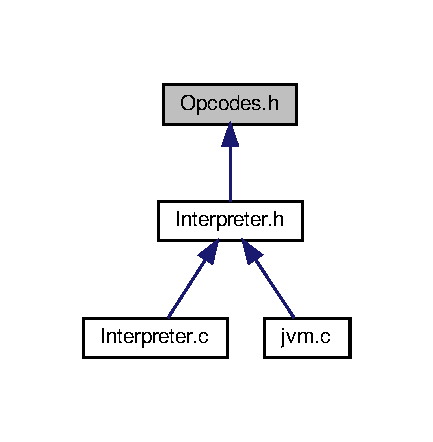
\includegraphics[width=208pt]{Opcodes_8h__dep__incl}
\end{center}
\end{figure}
\subsection*{Definições e Macros}
\begin{DoxyCompactItemize}
\item 
\#define \hyperlink{Opcodes_8h_abf43ce6eda0a748843a134d25e0fc671}{\+\_\+\+\_\+\+O\+P\+C\+O\+D\+E\+\_\+\+\_\+}
\end{DoxyCompactItemize}
\subsection*{Definições de Tipos}
\begin{DoxyCompactItemize}
\item 
typedef enum \hyperlink{Opcodes_8h_a299fc707c775371e0b2b0495ccb6158e}{opcode} \hyperlink{Opcodes_8h_a18fa3933ea0e15cfb3427323fa82d779}{opcodes}
\end{DoxyCompactItemize}
\subsection*{Enumerações}
\begin{DoxyCompactItemize}
\item 
enum \hyperlink{Opcodes_8h_a299fc707c775371e0b2b0495ccb6158e}{opcode} \{ \newline
\hyperlink{Opcodes_8h_a299fc707c775371e0b2b0495ccb6158ea700c6f9530feeed8d9ac947010f60ef5}{op\+\_\+nop} =0, 
\hyperlink{Opcodes_8h_a299fc707c775371e0b2b0495ccb6158eadfa0d74ab36f7118cf86e20d6fce4d6c}{op\+\_\+aconst\+\_\+null}, 
\hyperlink{Opcodes_8h_a299fc707c775371e0b2b0495ccb6158ea35c3359fbb592f12cfb18b526b07b444}{op\+\_\+iconst\+\_\+m1}, 
\hyperlink{Opcodes_8h_a299fc707c775371e0b2b0495ccb6158ea3ad48176e450d0aa4caea833a15bb79a}{op\+\_\+iconst\+\_\+0}, 
\newline
\hyperlink{Opcodes_8h_a299fc707c775371e0b2b0495ccb6158ea48728ff67c3d40f8478fec33b19b8617}{op\+\_\+iconst\+\_\+1}, 
\hyperlink{Opcodes_8h_a299fc707c775371e0b2b0495ccb6158ea3534d6c7710fea6fa65bccdfec08c648}{op\+\_\+iconst\+\_\+2}, 
\hyperlink{Opcodes_8h_a299fc707c775371e0b2b0495ccb6158ea4a62c9f38d1d65e690c9bf6b08636df6}{op\+\_\+iconst\+\_\+3}, 
\hyperlink{Opcodes_8h_a299fc707c775371e0b2b0495ccb6158ea9802d4d0290f37f47046adde53393da4}{op\+\_\+iconst\+\_\+4}, 
\newline
\hyperlink{Opcodes_8h_a299fc707c775371e0b2b0495ccb6158ea76038b2d448a0839454b1fcca7c54529}{op\+\_\+iconst\+\_\+5}, 
\hyperlink{Opcodes_8h_a299fc707c775371e0b2b0495ccb6158eae280452bd8a917527829926a4ad1b18a}{op\+\_\+lconst\+\_\+0}, 
\hyperlink{Opcodes_8h_a299fc707c775371e0b2b0495ccb6158ea9324491144d222cfa92edd7e44d1e4a5}{op\+\_\+lconst\+\_\+1}, 
\hyperlink{Opcodes_8h_a299fc707c775371e0b2b0495ccb6158ea5a9713b8df2cc3fce547d7961f7ec9a4}{op\+\_\+fconst\+\_\+0}, 
\newline
\hyperlink{Opcodes_8h_a299fc707c775371e0b2b0495ccb6158eaeacb237f31e3c72b5b6ae90daced8d81}{op\+\_\+fconst\+\_\+1}, 
\hyperlink{Opcodes_8h_a299fc707c775371e0b2b0495ccb6158ea85e1f41ed1152f898bd55cb326720142}{op\+\_\+fconst\+\_\+2}, 
\hyperlink{Opcodes_8h_a299fc707c775371e0b2b0495ccb6158ea5ccb2da2716cfe029a51261b646cbb59}{op\+\_\+dconst\+\_\+0}, 
\hyperlink{Opcodes_8h_a299fc707c775371e0b2b0495ccb6158eac725bfa59caeefdbc375f8a8aa047a48}{op\+\_\+dconst\+\_\+1}, 
\newline
\hyperlink{Opcodes_8h_a299fc707c775371e0b2b0495ccb6158ea4ca523db274f65c237100e3221fba4bb}{op\+\_\+bipush}, 
\hyperlink{Opcodes_8h_a299fc707c775371e0b2b0495ccb6158ea273af665ef704d35b1996737c4319757}{op\+\_\+sipush}, 
\hyperlink{Opcodes_8h_a299fc707c775371e0b2b0495ccb6158ea766f110e535f4957bbb61f39d2d3a5a8}{op\+\_\+ldc}, 
\hyperlink{Opcodes_8h_a299fc707c775371e0b2b0495ccb6158ead9aacf98b886bc00766d5f0ed38579db}{op\+\_\+ldc\+\_\+w}, 
\newline
\hyperlink{Opcodes_8h_a299fc707c775371e0b2b0495ccb6158ea607f19f4a13a3f92c1701c41ddcf56bb}{op\+\_\+ldc2\+\_\+w}, 
\hyperlink{Opcodes_8h_a299fc707c775371e0b2b0495ccb6158ea2dc065ad7be4a3f93f00de20b702c80a}{op\+\_\+iload}, 
\hyperlink{Opcodes_8h_a299fc707c775371e0b2b0495ccb6158ea07aa80d38dc785bf0d990f98f45cd506}{op\+\_\+lload}, 
\hyperlink{Opcodes_8h_a299fc707c775371e0b2b0495ccb6158eadb406faf5b7831065adf38ef066e8b22}{op\+\_\+fload}, 
\newline
\hyperlink{Opcodes_8h_a299fc707c775371e0b2b0495ccb6158ead7de738a5a0cda6e540acc938405e8aa}{op\+\_\+dload}, 
\hyperlink{Opcodes_8h_a299fc707c775371e0b2b0495ccb6158ea11400fc3ddc6647d44a67fdab026c740}{op\+\_\+aload}, 
\hyperlink{Opcodes_8h_a299fc707c775371e0b2b0495ccb6158ea321a9e43007951176a8ba09330610062}{op\+\_\+iload\+\_\+0}, 
\hyperlink{Opcodes_8h_a299fc707c775371e0b2b0495ccb6158ea26bef81ec37cf3a6165ba7991955f61e}{op\+\_\+iload\+\_\+1}, 
\newline
\hyperlink{Opcodes_8h_a299fc707c775371e0b2b0495ccb6158eae2b95b75d8429d02e0a797ad00215057}{op\+\_\+iload\+\_\+2}, 
\hyperlink{Opcodes_8h_a299fc707c775371e0b2b0495ccb6158ea22a2563f224d4272249a3c5b00e0e80a}{op\+\_\+iload\+\_\+3}, 
\hyperlink{Opcodes_8h_a299fc707c775371e0b2b0495ccb6158ea17b4e353e60f1f4de059fb3cdef67a9f}{op\+\_\+lload\+\_\+0}, 
\hyperlink{Opcodes_8h_a299fc707c775371e0b2b0495ccb6158ea65a99fdc8bd0cd45e075a158a1267cc4}{op\+\_\+lload\+\_\+1}, 
\newline
\hyperlink{Opcodes_8h_a299fc707c775371e0b2b0495ccb6158ea3217d901e0107c5d052d6d90c7a86fd1}{op\+\_\+lload\+\_\+2}, 
\hyperlink{Opcodes_8h_a299fc707c775371e0b2b0495ccb6158ead383b806c1c21c72a80af67547f93e76}{op\+\_\+lload\+\_\+3}, 
\hyperlink{Opcodes_8h_a299fc707c775371e0b2b0495ccb6158ea7ec1db4b200d5ac48b0956fdad27a674}{op\+\_\+fload\+\_\+0}, 
\hyperlink{Opcodes_8h_a299fc707c775371e0b2b0495ccb6158ea13e244fe85cb029032036b83bfa8475a}{op\+\_\+fload\+\_\+1}, 
\newline
\hyperlink{Opcodes_8h_a299fc707c775371e0b2b0495ccb6158ea239debf1ce21b13c72b0ccf25513b175}{op\+\_\+fload\+\_\+2}, 
\hyperlink{Opcodes_8h_a299fc707c775371e0b2b0495ccb6158ea24a9bf20eb4238aa774fbba520006717}{op\+\_\+fload\+\_\+3}, 
\hyperlink{Opcodes_8h_a299fc707c775371e0b2b0495ccb6158ea1577cacfe5392901606751a162501624}{op\+\_\+dload\+\_\+0}, 
\hyperlink{Opcodes_8h_a299fc707c775371e0b2b0495ccb6158ea2fd957370377da8712a46d1c2a9af1b0}{op\+\_\+dload\+\_\+1}, 
\newline
\hyperlink{Opcodes_8h_a299fc707c775371e0b2b0495ccb6158ea43fe683bb0179bb854212080d8f3344c}{op\+\_\+dload\+\_\+2}, 
\hyperlink{Opcodes_8h_a299fc707c775371e0b2b0495ccb6158ea34ca87c09c2ef4b2cf6be71945374a47}{op\+\_\+dload\+\_\+3}, 
\hyperlink{Opcodes_8h_a299fc707c775371e0b2b0495ccb6158ea137c430868b9627dea355f9d9c24677a}{op\+\_\+aload\+\_\+0}, 
\hyperlink{Opcodes_8h_a299fc707c775371e0b2b0495ccb6158ead2e79a613a4f8d2a50fdc4a2b833f0da}{op\+\_\+aload\+\_\+1}, 
\newline
\hyperlink{Opcodes_8h_a299fc707c775371e0b2b0495ccb6158ea5a3c5e803725ca4dd94ed50715b96566}{op\+\_\+aload\+\_\+2}, 
\hyperlink{Opcodes_8h_a299fc707c775371e0b2b0495ccb6158ea412c3365c53bf98e1541298f3d56fa41}{op\+\_\+aload\+\_\+3}, 
\hyperlink{Opcodes_8h_a299fc707c775371e0b2b0495ccb6158eab8569a75f82b5a0969e54a796c657c78}{op\+\_\+iaload}, 
\hyperlink{Opcodes_8h_a299fc707c775371e0b2b0495ccb6158ea8aa06fbeef7a585c2fe1016eba119446}{op\+\_\+laload}, 
\newline
\hyperlink{Opcodes_8h_a299fc707c775371e0b2b0495ccb6158eaf9fc21a59db7e95011ca96b789b0509e}{op\+\_\+faload}, 
\hyperlink{Opcodes_8h_a299fc707c775371e0b2b0495ccb6158ea59905fc4859c55c26f200f0744a9a672}{op\+\_\+daload}, 
\hyperlink{Opcodes_8h_a299fc707c775371e0b2b0495ccb6158ea3686fb0c77c2198130d87cb3dc82657c}{op\+\_\+aaload}, 
\hyperlink{Opcodes_8h_a299fc707c775371e0b2b0495ccb6158ea3d68a24c9d587ba0df820d9bf3dcba93}{op\+\_\+baload}, 
\newline
\hyperlink{Opcodes_8h_a299fc707c775371e0b2b0495ccb6158eaad25e37c4b7f3938348c21c89067432c}{op\+\_\+caload}, 
\hyperlink{Opcodes_8h_a299fc707c775371e0b2b0495ccb6158ea75c737818b7ffe282565d533fd63ff2e}{op\+\_\+saload}, 
\hyperlink{Opcodes_8h_a299fc707c775371e0b2b0495ccb6158ea0a29c47faefa42fa321b836317491fd4}{op\+\_\+istore}, 
\hyperlink{Opcodes_8h_a299fc707c775371e0b2b0495ccb6158ea3f9708a696346b0599017539be7be507}{op\+\_\+lstore}, 
\newline
\hyperlink{Opcodes_8h_a299fc707c775371e0b2b0495ccb6158eac7917d8854614c2a2d109fe776f1f462}{op\+\_\+fstore}, 
\hyperlink{Opcodes_8h_a299fc707c775371e0b2b0495ccb6158ea76caeda8e8c35db7731cbdefc6eae6f7}{op\+\_\+dstore}, 
\hyperlink{Opcodes_8h_a299fc707c775371e0b2b0495ccb6158eac37db0771978170dae1f8c39e0e272e0}{op\+\_\+astore}, 
\hyperlink{Opcodes_8h_a299fc707c775371e0b2b0495ccb6158ea39844703c5504ea34b89c91ce662a056}{op\+\_\+istore\+\_\+0}, 
\newline
\hyperlink{Opcodes_8h_a299fc707c775371e0b2b0495ccb6158ea945b493101e84ed169f0d4c10475cc1d}{op\+\_\+istore\+\_\+1}, 
\hyperlink{Opcodes_8h_a299fc707c775371e0b2b0495ccb6158ea2be206892117def0165bc13ecec1f281}{op\+\_\+istore\+\_\+2}, 
\hyperlink{Opcodes_8h_a299fc707c775371e0b2b0495ccb6158ea0985638583496d73e8deef5f1dbe7223}{op\+\_\+istore\+\_\+3}, 
\hyperlink{Opcodes_8h_a299fc707c775371e0b2b0495ccb6158eab57540e18344ea34b97639cee61a7959}{op\+\_\+lstore\+\_\+0}, 
\newline
\hyperlink{Opcodes_8h_a299fc707c775371e0b2b0495ccb6158eacbcaaf9e9db0bc277db3de2f90179b7e}{op\+\_\+lstore\+\_\+1}, 
\hyperlink{Opcodes_8h_a299fc707c775371e0b2b0495ccb6158eacd105c5cfaccf458717945a65f3b8745}{op\+\_\+lstore\+\_\+2}, 
\hyperlink{Opcodes_8h_a299fc707c775371e0b2b0495ccb6158ea55a0e4f9ebc64e175cde868ea6e92b72}{op\+\_\+lstore\+\_\+3}, 
\hyperlink{Opcodes_8h_a299fc707c775371e0b2b0495ccb6158eae66261a791864c5a2e41a3e3d0fd9619}{op\+\_\+fstore\+\_\+0}, 
\newline
\hyperlink{Opcodes_8h_a299fc707c775371e0b2b0495ccb6158ea43c7076e802734425015684b8a7472c3}{op\+\_\+fstore\+\_\+1}, 
\hyperlink{Opcodes_8h_a299fc707c775371e0b2b0495ccb6158ea0e42e555884762b014135f8b0b0dd63f}{op\+\_\+fstore\+\_\+2}, 
\hyperlink{Opcodes_8h_a299fc707c775371e0b2b0495ccb6158eacaa85c214e4f6ec6ea5359ad24e2fc2f}{op\+\_\+fstore\+\_\+3}, 
\hyperlink{Opcodes_8h_a299fc707c775371e0b2b0495ccb6158ea84e0a81725cdc1913c8868f081833265}{op\+\_\+dstore\+\_\+0}, 
\newline
\hyperlink{Opcodes_8h_a299fc707c775371e0b2b0495ccb6158eab21095f623c6a565ce81e775ef958364}{op\+\_\+dstore\+\_\+1}, 
\hyperlink{Opcodes_8h_a299fc707c775371e0b2b0495ccb6158ea6d40c9ebe596fde840f6a62c7ba1bb86}{op\+\_\+dstore\+\_\+2}, 
\hyperlink{Opcodes_8h_a299fc707c775371e0b2b0495ccb6158ea50e1ec29c0510cd3a66ecefe752791dc}{op\+\_\+dstore\+\_\+3}, 
\hyperlink{Opcodes_8h_a299fc707c775371e0b2b0495ccb6158ea7caece879c9940e10c02a56ed03cf937}{op\+\_\+astore\+\_\+0}, 
\newline
\hyperlink{Opcodes_8h_a299fc707c775371e0b2b0495ccb6158eaa2a33fa280d67234d3e6976ec4531e8a}{op\+\_\+astore\+\_\+1}, 
\hyperlink{Opcodes_8h_a299fc707c775371e0b2b0495ccb6158ea3ad5c60a897f07ec67bd786a4b62d05f}{op\+\_\+astore\+\_\+2}, 
\hyperlink{Opcodes_8h_a299fc707c775371e0b2b0495ccb6158ea13921d82785cbc3ef6c766903c6c62b6}{op\+\_\+astore\+\_\+3}, 
\hyperlink{Opcodes_8h_a299fc707c775371e0b2b0495ccb6158eadd14f363b600a4fef39304cdd74cc4c1}{op\+\_\+iastore}, 
\newline
\hyperlink{Opcodes_8h_a299fc707c775371e0b2b0495ccb6158ea9fea452815c1987ecd113c6ad0cfd947}{op\+\_\+lastore}, 
\hyperlink{Opcodes_8h_a299fc707c775371e0b2b0495ccb6158ea6ff49c30408ee3b1905775cc8502af1d}{op\+\_\+fastore}, 
\hyperlink{Opcodes_8h_a299fc707c775371e0b2b0495ccb6158ea2a0f2e05fe785284d2a35a98ecf01bd8}{op\+\_\+dastore}, 
\hyperlink{Opcodes_8h_a299fc707c775371e0b2b0495ccb6158eaa3c233f2735d0b2e111f35e320114ae6}{op\+\_\+aastore}, 
\newline
\hyperlink{Opcodes_8h_a299fc707c775371e0b2b0495ccb6158eaffe95ec1189f0b114e87ec7f1ff612d1}{op\+\_\+bastore}, 
\hyperlink{Opcodes_8h_a299fc707c775371e0b2b0495ccb6158ead365cdc16e507957d5693c16c76b7513}{op\+\_\+castore}, 
\hyperlink{Opcodes_8h_a299fc707c775371e0b2b0495ccb6158eaafba8b6c84a1a27770aa1c9f8f5589d3}{op\+\_\+sastore}, 
\hyperlink{Opcodes_8h_a299fc707c775371e0b2b0495ccb6158eaab21e52698f7aad5c5d1a2189b757481}{op\+\_\+pop}, 
\newline
\hyperlink{Opcodes_8h_a299fc707c775371e0b2b0495ccb6158eab6b3d76f40d556df2d287c9af2a5f2a1}{op\+\_\+pop2}, 
\hyperlink{Opcodes_8h_a299fc707c775371e0b2b0495ccb6158eaafa0542ef3cfa5c679c997277ee83fea}{op\+\_\+dup}, 
\hyperlink{Opcodes_8h_a299fc707c775371e0b2b0495ccb6158ea22680f488cfd14110fa1387d8592a619}{op\+\_\+dup\+\_\+x1}, 
\hyperlink{Opcodes_8h_a299fc707c775371e0b2b0495ccb6158ea36fe9d5a58a9f36eeb611b4ca981d092}{op\+\_\+dup\+\_\+x2}, 
\newline
\hyperlink{Opcodes_8h_a299fc707c775371e0b2b0495ccb6158eaf048bcacc92aeb315dfac3897e6391ce}{op\+\_\+dup2}, 
\hyperlink{Opcodes_8h_a299fc707c775371e0b2b0495ccb6158eab7a27be1f25dac3955e79cd1020bedf5}{op\+\_\+dup2\+\_\+x1}, 
\hyperlink{Opcodes_8h_a299fc707c775371e0b2b0495ccb6158ea7dd127028fd28e274abccb7077c8b5be}{op\+\_\+dup2\+\_\+x2}, 
\hyperlink{Opcodes_8h_a299fc707c775371e0b2b0495ccb6158ea4f909a59c91bab4039e0951743e52769}{op\+\_\+swap}, 
\newline
\hyperlink{Opcodes_8h_a299fc707c775371e0b2b0495ccb6158ea39d1a4e014990f2c1c543357883aeb68}{op\+\_\+iadd}, 
\hyperlink{Opcodes_8h_a299fc707c775371e0b2b0495ccb6158ead59b2cd6292418ca19256c374be8c18a}{op\+\_\+ladd}, 
\hyperlink{Opcodes_8h_a299fc707c775371e0b2b0495ccb6158ea979aca7a567d6e1640078e5b5490e236}{op\+\_\+fadd}, 
\hyperlink{Opcodes_8h_a299fc707c775371e0b2b0495ccb6158ea58fb540d706eb6861f2f62c3e775f7b2}{op\+\_\+dadd}, 
\newline
\hyperlink{Opcodes_8h_a299fc707c775371e0b2b0495ccb6158ea3da3a0948a3cee481e19f1b202bf0b51}{op\+\_\+isub}, 
\hyperlink{Opcodes_8h_a299fc707c775371e0b2b0495ccb6158ea3d1f594f345bf8c61916416a45364909}{op\+\_\+lsub}, 
\hyperlink{Opcodes_8h_a299fc707c775371e0b2b0495ccb6158ea43d9ec0154aaca24bd94a40a5bb2d785}{op\+\_\+fsub}, 
\hyperlink{Opcodes_8h_a299fc707c775371e0b2b0495ccb6158ea630d980326402dbd2f5d6f1e735dc696}{op\+\_\+dsub}, 
\newline
\hyperlink{Opcodes_8h_a299fc707c775371e0b2b0495ccb6158ea54d8bc8f4055376a41a9e4f271bb00dc}{op\+\_\+imul}, 
\hyperlink{Opcodes_8h_a299fc707c775371e0b2b0495ccb6158ea9ea1f43b35b88e78f81a48fce3ea3346}{op\+\_\+lmul}, 
\hyperlink{Opcodes_8h_a299fc707c775371e0b2b0495ccb6158ea44ce5bba8b427a263d3fc0daf092f6b2}{op\+\_\+fmul}, 
\hyperlink{Opcodes_8h_a299fc707c775371e0b2b0495ccb6158ea917037dec2ffc5ee6689530304c334cb}{op\+\_\+dmul}, 
\newline
\hyperlink{Opcodes_8h_a299fc707c775371e0b2b0495ccb6158eaf6dcacc56d410161d4762b3faec0f86e}{op\+\_\+idiv}, 
\hyperlink{Opcodes_8h_a299fc707c775371e0b2b0495ccb6158ea1d6c377bab0629486e6a65e03048e440}{op\+\_\+ldiv}, 
\hyperlink{Opcodes_8h_a299fc707c775371e0b2b0495ccb6158ea80f56745e3cdefdf990333214a16c415}{op\+\_\+fdiv}, 
\hyperlink{Opcodes_8h_a299fc707c775371e0b2b0495ccb6158eacc5e267a113ce287542bf66c55a73954}{op\+\_\+ddiv}, 
\newline
\hyperlink{Opcodes_8h_a299fc707c775371e0b2b0495ccb6158ea4dedb12c7b6350c25d8d6a70d9549bb8}{op\+\_\+irem}, 
\hyperlink{Opcodes_8h_a299fc707c775371e0b2b0495ccb6158ea3c72ba11a6d6ab508b25ec706882f02b}{op\+\_\+lrem}, 
\hyperlink{Opcodes_8h_a299fc707c775371e0b2b0495ccb6158ea7f5de0081a39a4f320dacf27e1b131ba}{op\+\_\+frem}, 
\hyperlink{Opcodes_8h_a299fc707c775371e0b2b0495ccb6158eaec7b8a67e103d43e9e4d00fbf7a3c82c}{op\+\_\+drem}, 
\newline
\hyperlink{Opcodes_8h_a299fc707c775371e0b2b0495ccb6158eaa9eafd487c1d45ec6a921e535ed0cd0c}{op\+\_\+ineg}, 
\hyperlink{Opcodes_8h_a299fc707c775371e0b2b0495ccb6158ea92cfd18f1e2be8dbb328a5378a921e70}{op\+\_\+lneg}, 
\hyperlink{Opcodes_8h_a299fc707c775371e0b2b0495ccb6158ea44df0f6ce90d41570404c9bffe5af6b4}{op\+\_\+fneg}, 
\hyperlink{Opcodes_8h_a299fc707c775371e0b2b0495ccb6158ea62ff320c91dd5a57dde1e1c09033838a}{op\+\_\+dneg}, 
\newline
\hyperlink{Opcodes_8h_a299fc707c775371e0b2b0495ccb6158ea27ee5d1bb1ae07e5b0a221b41f694427}{op\+\_\+ishl}, 
\hyperlink{Opcodes_8h_a299fc707c775371e0b2b0495ccb6158ea3cf99f399f0d85f79e1f3d4db12a4993}{op\+\_\+lshl}, 
\hyperlink{Opcodes_8h_a299fc707c775371e0b2b0495ccb6158ea7342f726f5b250e35ec125e670678854}{op\+\_\+ishr}, 
\hyperlink{Opcodes_8h_a299fc707c775371e0b2b0495ccb6158ea4755d7063c3cd66437092d4115b253a7}{op\+\_\+lshr}, 
\newline
\hyperlink{Opcodes_8h_a299fc707c775371e0b2b0495ccb6158eaa179a95431e16f7ed0d5fe0349564c91}{op\+\_\+iushr}, 
\hyperlink{Opcodes_8h_a299fc707c775371e0b2b0495ccb6158ea417a0cbd6b00cbe5791f3adf16a2e433}{op\+\_\+lushr}, 
\hyperlink{Opcodes_8h_a299fc707c775371e0b2b0495ccb6158eaea0b949fc5a86e83e6803cc19972162b}{op\+\_\+iand}, 
\hyperlink{Opcodes_8h_a299fc707c775371e0b2b0495ccb6158ea2830ffbec88e4135ad0847723bef5751}{op\+\_\+land}, 
\newline
\hyperlink{Opcodes_8h_a299fc707c775371e0b2b0495ccb6158ea4f3288dc88ca60cbed284ec9096e016a}{op\+\_\+ior}, 
\hyperlink{Opcodes_8h_a299fc707c775371e0b2b0495ccb6158ea4767a4b974fab30e6046071d6d340ef5}{op\+\_\+lor}, 
\hyperlink{Opcodes_8h_a299fc707c775371e0b2b0495ccb6158eabf390ddec4993f5cda621e1a05238020}{op\+\_\+ixor}, 
\hyperlink{Opcodes_8h_a299fc707c775371e0b2b0495ccb6158ea0bd9593d8c544f8335a37bffaef51140}{op\+\_\+lxor}, 
\newline
\hyperlink{Opcodes_8h_a299fc707c775371e0b2b0495ccb6158eae2a94821875a6137939df49122c51523}{op\+\_\+iinc}, 
\hyperlink{Opcodes_8h_a299fc707c775371e0b2b0495ccb6158ea963815fedb0fed9d71549b796fa3ab73}{op\+\_\+i2l}, 
\hyperlink{Opcodes_8h_a299fc707c775371e0b2b0495ccb6158ea9df27041000de47a412bd6a655f3e51d}{op\+\_\+i2f}, 
\hyperlink{Opcodes_8h_a299fc707c775371e0b2b0495ccb6158ea15b338f7684c92f7e0ebfe0102af820d}{op\+\_\+i2d}, 
\newline
\hyperlink{Opcodes_8h_a299fc707c775371e0b2b0495ccb6158ea4d6b9056fa9bc7f102ac4b1f4d8b0a48}{op\+\_\+l2i}, 
\hyperlink{Opcodes_8h_a299fc707c775371e0b2b0495ccb6158eaa594a6e7813b2470c4b0395f3a51b2fd}{op\+\_\+l2f}, 
\hyperlink{Opcodes_8h_a299fc707c775371e0b2b0495ccb6158ea4414a13e84d4dfbd90e1cfda955237c4}{op\+\_\+l2d}, 
\hyperlink{Opcodes_8h_a299fc707c775371e0b2b0495ccb6158eaead12b40c01b684d3b114a26af938829}{op\+\_\+f2i}, 
\newline
\hyperlink{Opcodes_8h_a299fc707c775371e0b2b0495ccb6158ea6ed4deccd3d8ab92b8293eec9c2648ca}{op\+\_\+f2l}, 
\hyperlink{Opcodes_8h_a299fc707c775371e0b2b0495ccb6158ea0f4210ce71a5eb6520fc7f0a7deee070}{op\+\_\+f2d}, 
\hyperlink{Opcodes_8h_a299fc707c775371e0b2b0495ccb6158ead0b89c888220dcb8704c2556fa43b2fa}{op\+\_\+d2i}, 
\hyperlink{Opcodes_8h_a299fc707c775371e0b2b0495ccb6158ea2a7800a586ab3372e15c02c409a0ca42}{op\+\_\+d2l}, 
\newline
\hyperlink{Opcodes_8h_a299fc707c775371e0b2b0495ccb6158ea7645cf8ba133e17a20a9b3e987fe30f1}{op\+\_\+d2f}, 
\hyperlink{Opcodes_8h_a299fc707c775371e0b2b0495ccb6158ea956aa66237d1674987611075098ceecf}{op\+\_\+i2b}, 
\hyperlink{Opcodes_8h_a299fc707c775371e0b2b0495ccb6158ea6b23288fe87d0d7c654d33a9a35bebb6}{op\+\_\+i2c}, 
\hyperlink{Opcodes_8h_a299fc707c775371e0b2b0495ccb6158ea251174f1940181e6c5d7ac72616a6409}{op\+\_\+i2s}, 
\newline
\hyperlink{Opcodes_8h_a299fc707c775371e0b2b0495ccb6158ea837336460e95938a65177810e91f767e}{op\+\_\+lcmp}, 
\hyperlink{Opcodes_8h_a299fc707c775371e0b2b0495ccb6158eac016d336eaf3a76b21525b1899615cb1}{op\+\_\+fcmpl}, 
\hyperlink{Opcodes_8h_a299fc707c775371e0b2b0495ccb6158ea9e8ea464f52edb25e9c24f66daa6b357}{op\+\_\+fcmpg}, 
\hyperlink{Opcodes_8h_a299fc707c775371e0b2b0495ccb6158ea226e94357f4eceb4f621f51a57fed033}{op\+\_\+dcmpl}, 
\newline
\hyperlink{Opcodes_8h_a299fc707c775371e0b2b0495ccb6158ea3144397fe2ab5388b2b94eb4ae692b6c}{op\+\_\+dcmpg}, 
\hyperlink{Opcodes_8h_a299fc707c775371e0b2b0495ccb6158ea40fc61fa0640ab9d1b9850a532823202}{op\+\_\+ifeq}, 
\hyperlink{Opcodes_8h_a299fc707c775371e0b2b0495ccb6158ead62645dbaf33f9c49f1a1b60ad296513}{op\+\_\+ifne}, 
\hyperlink{Opcodes_8h_a299fc707c775371e0b2b0495ccb6158eac1ef2a83ec1ca84d95c29a32988f05f8}{op\+\_\+iflt}, 
\newline
\hyperlink{Opcodes_8h_a299fc707c775371e0b2b0495ccb6158ea19eea9e2c8cfe27d5cf11b6dd1b96370}{op\+\_\+ifge}, 
\hyperlink{Opcodes_8h_a299fc707c775371e0b2b0495ccb6158ea0fc621796e6965ef1741fcdbaad96e4a}{op\+\_\+ifgt}, 
\hyperlink{Opcodes_8h_a299fc707c775371e0b2b0495ccb6158eaf374b86e383abe821f2ddbe3b4e09c02}{op\+\_\+ifle}, 
\hyperlink{Opcodes_8h_a299fc707c775371e0b2b0495ccb6158ea6d05469e455d8bcd2306220f09038218}{op\+\_\+if\+\_\+icmpeq}, 
\newline
\hyperlink{Opcodes_8h_a299fc707c775371e0b2b0495ccb6158ea25c210781a484fcd1f4594e8b18c75f5}{op\+\_\+if\+\_\+icmpne}, 
\hyperlink{Opcodes_8h_a299fc707c775371e0b2b0495ccb6158eae0192b9a9c9c27def84b1ed95a5e101e}{op\+\_\+if\+\_\+icmplt}, 
\hyperlink{Opcodes_8h_a299fc707c775371e0b2b0495ccb6158eab0a01f383418cad9039dc2d105858adf}{op\+\_\+if\+\_\+icmpge}, 
\hyperlink{Opcodes_8h_a299fc707c775371e0b2b0495ccb6158eaaa142be0793faf3ea3ed47ec035320a9}{op\+\_\+if\+\_\+icmpgt}, 
\newline
\hyperlink{Opcodes_8h_a299fc707c775371e0b2b0495ccb6158eafb5d3d7cce44b8647dfd2e41d6458505}{op\+\_\+if\+\_\+icmple}, 
\hyperlink{Opcodes_8h_a299fc707c775371e0b2b0495ccb6158ea4ad1fb4c80b86efa7da0a63d4ad64700}{op\+\_\+if\+\_\+acmpeq}, 
\hyperlink{Opcodes_8h_a299fc707c775371e0b2b0495ccb6158ea9b7b4cd5705afdd72f1968b692e6558f}{op\+\_\+if\+\_\+acmpne}, 
\hyperlink{Opcodes_8h_a299fc707c775371e0b2b0495ccb6158ea820250588e75e19630eed2875b3bd636}{op\+\_\+goto}, 
\newline
\hyperlink{Opcodes_8h_a299fc707c775371e0b2b0495ccb6158ea941f9861ee7080f8bb5f1534d947da53}{op\+\_\+jsr}, 
\hyperlink{Opcodes_8h_a299fc707c775371e0b2b0495ccb6158eaee10a5803332851c406c1e2389bdc508}{op\+\_\+ret}, 
\hyperlink{Opcodes_8h_a299fc707c775371e0b2b0495ccb6158ea28465f9c21e31f2d5fdf090690135e73}{op\+\_\+tableswitch}, 
\hyperlink{Opcodes_8h_a299fc707c775371e0b2b0495ccb6158eafd4429c2b7ef6d367bd339ac5ec5e723}{op\+\_\+lookupswitch}, 
\newline
\hyperlink{Opcodes_8h_a299fc707c775371e0b2b0495ccb6158ea11d64b209a7bb41583802664dd9d1e4c}{op\+\_\+ireturn}, 
\hyperlink{Opcodes_8h_a299fc707c775371e0b2b0495ccb6158eab6ef2e91af361c944f88a9ace7d7a91b}{op\+\_\+lreturn}, 
\hyperlink{Opcodes_8h_a299fc707c775371e0b2b0495ccb6158ea1b6cfa102249e60cc2fe77af232da21e}{op\+\_\+freturn}, 
\hyperlink{Opcodes_8h_a299fc707c775371e0b2b0495ccb6158ea00fda44ce170c3adbe6c1bd35d9be632}{op\+\_\+dreturn}, 
\newline
\hyperlink{Opcodes_8h_a299fc707c775371e0b2b0495ccb6158ea78d0674c4c2733a4cc16431177646418}{op\+\_\+areturn}, 
\hyperlink{Opcodes_8h_a299fc707c775371e0b2b0495ccb6158eae2db67096cdbc6de46fa341942e1898d}{op\+\_\+return}, 
\hyperlink{Opcodes_8h_a299fc707c775371e0b2b0495ccb6158eae7cc96036e7151c169d9523ff0f4bd13}{op\+\_\+getstatic}, 
\hyperlink{Opcodes_8h_a299fc707c775371e0b2b0495ccb6158ea3699ce55906da34b0d4103c45e835e8a}{op\+\_\+putstatic}, 
\newline
\hyperlink{Opcodes_8h_a299fc707c775371e0b2b0495ccb6158ea852e2f759a1612e20adf8e0a16aa493a}{op\+\_\+getfield}, 
\hyperlink{Opcodes_8h_a299fc707c775371e0b2b0495ccb6158ea3f01ea8cd057b8eb6fb49c01e45eb08c}{op\+\_\+putfield}, 
\hyperlink{Opcodes_8h_a299fc707c775371e0b2b0495ccb6158ead84fc577fb10b44fc0905af71bf7262e}{op\+\_\+invokevirtual}, 
\hyperlink{Opcodes_8h_a299fc707c775371e0b2b0495ccb6158ea112bd7bad0142c05b6080af8550732ae}{op\+\_\+invokespecial}, 
\newline
\hyperlink{Opcodes_8h_a299fc707c775371e0b2b0495ccb6158ea7f2f7e91856479a94de2f02a490bb528}{op\+\_\+invokestatic}, 
\hyperlink{Opcodes_8h_a299fc707c775371e0b2b0495ccb6158eaf90bacc5369066ebcad5a885ef63a8d1}{op\+\_\+invokeinterface}, 
\hyperlink{Opcodes_8h_a299fc707c775371e0b2b0495ccb6158ea28b3a77c17fd40f25508570aca22e606}{op\+\_\+xxxunusedxxx1}, 
\hyperlink{Opcodes_8h_a299fc707c775371e0b2b0495ccb6158ea8a2a233b03256677662392e73095d1d5}{op\+\_\+new}, 
\newline
\hyperlink{Opcodes_8h_a299fc707c775371e0b2b0495ccb6158ead49537264a415937e52cc52996fa45c6}{op\+\_\+newarray}, 
\hyperlink{Opcodes_8h_a299fc707c775371e0b2b0495ccb6158eacd6136082db3c0838fa993e5e36032d1}{op\+\_\+anewarray}, 
\hyperlink{Opcodes_8h_a299fc707c775371e0b2b0495ccb6158ea4c4eab84410ef632110040745394bbbd}{op\+\_\+arraylength}, 
\hyperlink{Opcodes_8h_a299fc707c775371e0b2b0495ccb6158eaafe64d6ed91bc6a5705c4e3af152a7ba}{op\+\_\+athrow}, 
\newline
\hyperlink{Opcodes_8h_a299fc707c775371e0b2b0495ccb6158ea0fe84d761b96db805c0a71f418591e95}{op\+\_\+checkcast}, 
\hyperlink{Opcodes_8h_a299fc707c775371e0b2b0495ccb6158ea9e41ca35d95ae3abe9d2a89772e2730c}{op\+\_\+instanceof}, 
\hyperlink{Opcodes_8h_a299fc707c775371e0b2b0495ccb6158ea8e783f4680d426e5a11e8274cc28b6e0}{op\+\_\+monitorenter}, 
\hyperlink{Opcodes_8h_a299fc707c775371e0b2b0495ccb6158ea1271b0cbc8ff5f8405076e9b20a930f2}{op\+\_\+monitorexit}, 
\newline
\hyperlink{Opcodes_8h_a299fc707c775371e0b2b0495ccb6158ea8cd8c8fdd18d755fdde73f9d17c454e6}{op\+\_\+wide}, 
\hyperlink{Opcodes_8h_a299fc707c775371e0b2b0495ccb6158ea31c3995ca080a8ed46ffaa0e76974c09}{op\+\_\+multianewarray}, 
\hyperlink{Opcodes_8h_a299fc707c775371e0b2b0495ccb6158ea0f62e70bb07a1e157a1d3bf3df5d02d1}{op\+\_\+ifnull}, 
\hyperlink{Opcodes_8h_a299fc707c775371e0b2b0495ccb6158eaadbca4b9e28350dbc5e747e6c64d2f43}{op\+\_\+ifnonnull}, 
\newline
\hyperlink{Opcodes_8h_a299fc707c775371e0b2b0495ccb6158eaa1c6de1e49983e57e37ab09040b7506d}{op\+\_\+goto\+\_\+w}, 
\hyperlink{Opcodes_8h_a299fc707c775371e0b2b0495ccb6158eaa9343b27d1787d54068daea6adfd1a46}{op\+\_\+jsr\+\_\+w}, 
\hyperlink{Opcodes_8h_a299fc707c775371e0b2b0495ccb6158ea6afe512f8589cf42ee4cd0c7d4354326}{op\+\_\+breakpoint}, 
\hyperlink{Opcodes_8h_a299fc707c775371e0b2b0495ccb6158ea0d8712b40683fdef11e9585b0b32f48e}{op\+\_\+impdep1} = 254, 
\newline
\hyperlink{Opcodes_8h_a299fc707c775371e0b2b0495ccb6158eac594baced688f108d6dfeefd6138dc6c}{op\+\_\+impdep}
 \}
\end{DoxyCompactItemize}


\subsection{Definições e macros}
\mbox{\Hypertarget{Opcodes_8h_abf43ce6eda0a748843a134d25e0fc671}\label{Opcodes_8h_abf43ce6eda0a748843a134d25e0fc671}} 
\index{Opcodes.\+h@{Opcodes.\+h}!\+\_\+\+\_\+\+O\+P\+C\+O\+D\+E\+\_\+\+\_\+@{\+\_\+\+\_\+\+O\+P\+C\+O\+D\+E\+\_\+\+\_\+}}
\index{\+\_\+\+\_\+\+O\+P\+C\+O\+D\+E\+\_\+\+\_\+@{\+\_\+\+\_\+\+O\+P\+C\+O\+D\+E\+\_\+\+\_\+}!Opcodes.\+h@{Opcodes.\+h}}
\subsubsection{\texorpdfstring{\+\_\+\+\_\+\+O\+P\+C\+O\+D\+E\+\_\+\+\_\+}{\_\_OPCODE\_\_}}
{\footnotesize\ttfamily \#define \+\_\+\+\_\+\+O\+P\+C\+O\+D\+E\+\_\+\+\_\+}



\subsection{Definições dos tipos}
\mbox{\Hypertarget{Opcodes_8h_a18fa3933ea0e15cfb3427323fa82d779}\label{Opcodes_8h_a18fa3933ea0e15cfb3427323fa82d779}} 
\index{Opcodes.\+h@{Opcodes.\+h}!opcodes@{opcodes}}
\index{opcodes@{opcodes}!Opcodes.\+h@{Opcodes.\+h}}
\subsubsection{\texorpdfstring{opcodes}{opcodes}}
{\footnotesize\ttfamily typedef enum \hyperlink{Opcodes_8h_a299fc707c775371e0b2b0495ccb6158e}{opcode}  \hyperlink{Opcodes_8h_a18fa3933ea0e15cfb3427323fa82d779}{opcodes}}



\subsection{Enumerações}
\mbox{\Hypertarget{Opcodes_8h_a299fc707c775371e0b2b0495ccb6158e}\label{Opcodes_8h_a299fc707c775371e0b2b0495ccb6158e}} 
\index{Opcodes.\+h@{Opcodes.\+h}!opcode@{opcode}}
\index{opcode@{opcode}!Opcodes.\+h@{Opcodes.\+h}}
\subsubsection{\texorpdfstring{opcode}{opcode}}
{\footnotesize\ttfamily enum \hyperlink{Opcodes_8h_a299fc707c775371e0b2b0495ccb6158e}{opcode}}

\begin{DoxyEnumFields}{Valores de enumerações}
\raisebox{\heightof{T}}[0pt][0pt]{\index{op\+\_\+nop@{op\+\_\+nop}!Opcodes.\+h@{Opcodes.\+h}}\index{Opcodes.\+h@{Opcodes.\+h}!op\+\_\+nop@{op\+\_\+nop}}}\mbox{\Hypertarget{Opcodes_8h_a299fc707c775371e0b2b0495ccb6158ea700c6f9530feeed8d9ac947010f60ef5}\label{Opcodes_8h_a299fc707c775371e0b2b0495ccb6158ea700c6f9530feeed8d9ac947010f60ef5}} 
op\+\_\+nop&\\
\hline

\raisebox{\heightof{T}}[0pt][0pt]{\index{op\+\_\+aconst\+\_\+null@{op\+\_\+aconst\+\_\+null}!Opcodes.\+h@{Opcodes.\+h}}\index{Opcodes.\+h@{Opcodes.\+h}!op\+\_\+aconst\+\_\+null@{op\+\_\+aconst\+\_\+null}}}\mbox{\Hypertarget{Opcodes_8h_a299fc707c775371e0b2b0495ccb6158eadfa0d74ab36f7118cf86e20d6fce4d6c}\label{Opcodes_8h_a299fc707c775371e0b2b0495ccb6158eadfa0d74ab36f7118cf86e20d6fce4d6c}} 
op\+\_\+aconst\+\_\+null&\\
\hline

\raisebox{\heightof{T}}[0pt][0pt]{\index{op\+\_\+iconst\+\_\+m1@{op\+\_\+iconst\+\_\+m1}!Opcodes.\+h@{Opcodes.\+h}}\index{Opcodes.\+h@{Opcodes.\+h}!op\+\_\+iconst\+\_\+m1@{op\+\_\+iconst\+\_\+m1}}}\mbox{\Hypertarget{Opcodes_8h_a299fc707c775371e0b2b0495ccb6158ea35c3359fbb592f12cfb18b526b07b444}\label{Opcodes_8h_a299fc707c775371e0b2b0495ccb6158ea35c3359fbb592f12cfb18b526b07b444}} 
op\+\_\+iconst\+\_\+m1&\\
\hline

\raisebox{\heightof{T}}[0pt][0pt]{\index{op\+\_\+iconst\+\_\+0@{op\+\_\+iconst\+\_\+0}!Opcodes.\+h@{Opcodes.\+h}}\index{Opcodes.\+h@{Opcodes.\+h}!op\+\_\+iconst\+\_\+0@{op\+\_\+iconst\+\_\+0}}}\mbox{\Hypertarget{Opcodes_8h_a299fc707c775371e0b2b0495ccb6158ea3ad48176e450d0aa4caea833a15bb79a}\label{Opcodes_8h_a299fc707c775371e0b2b0495ccb6158ea3ad48176e450d0aa4caea833a15bb79a}} 
op\+\_\+iconst\+\_\+0&\\
\hline

\raisebox{\heightof{T}}[0pt][0pt]{\index{op\+\_\+iconst\+\_\+1@{op\+\_\+iconst\+\_\+1}!Opcodes.\+h@{Opcodes.\+h}}\index{Opcodes.\+h@{Opcodes.\+h}!op\+\_\+iconst\+\_\+1@{op\+\_\+iconst\+\_\+1}}}\mbox{\Hypertarget{Opcodes_8h_a299fc707c775371e0b2b0495ccb6158ea48728ff67c3d40f8478fec33b19b8617}\label{Opcodes_8h_a299fc707c775371e0b2b0495ccb6158ea48728ff67c3d40f8478fec33b19b8617}} 
op\+\_\+iconst\+\_\+1&\\
\hline

\raisebox{\heightof{T}}[0pt][0pt]{\index{op\+\_\+iconst\+\_\+2@{op\+\_\+iconst\+\_\+2}!Opcodes.\+h@{Opcodes.\+h}}\index{Opcodes.\+h@{Opcodes.\+h}!op\+\_\+iconst\+\_\+2@{op\+\_\+iconst\+\_\+2}}}\mbox{\Hypertarget{Opcodes_8h_a299fc707c775371e0b2b0495ccb6158ea3534d6c7710fea6fa65bccdfec08c648}\label{Opcodes_8h_a299fc707c775371e0b2b0495ccb6158ea3534d6c7710fea6fa65bccdfec08c648}} 
op\+\_\+iconst\+\_\+2&\\
\hline

\raisebox{\heightof{T}}[0pt][0pt]{\index{op\+\_\+iconst\+\_\+3@{op\+\_\+iconst\+\_\+3}!Opcodes.\+h@{Opcodes.\+h}}\index{Opcodes.\+h@{Opcodes.\+h}!op\+\_\+iconst\+\_\+3@{op\+\_\+iconst\+\_\+3}}}\mbox{\Hypertarget{Opcodes_8h_a299fc707c775371e0b2b0495ccb6158ea4a62c9f38d1d65e690c9bf6b08636df6}\label{Opcodes_8h_a299fc707c775371e0b2b0495ccb6158ea4a62c9f38d1d65e690c9bf6b08636df6}} 
op\+\_\+iconst\+\_\+3&\\
\hline

\raisebox{\heightof{T}}[0pt][0pt]{\index{op\+\_\+iconst\+\_\+4@{op\+\_\+iconst\+\_\+4}!Opcodes.\+h@{Opcodes.\+h}}\index{Opcodes.\+h@{Opcodes.\+h}!op\+\_\+iconst\+\_\+4@{op\+\_\+iconst\+\_\+4}}}\mbox{\Hypertarget{Opcodes_8h_a299fc707c775371e0b2b0495ccb6158ea9802d4d0290f37f47046adde53393da4}\label{Opcodes_8h_a299fc707c775371e0b2b0495ccb6158ea9802d4d0290f37f47046adde53393da4}} 
op\+\_\+iconst\+\_\+4&\\
\hline

\raisebox{\heightof{T}}[0pt][0pt]{\index{op\+\_\+iconst\+\_\+5@{op\+\_\+iconst\+\_\+5}!Opcodes.\+h@{Opcodes.\+h}}\index{Opcodes.\+h@{Opcodes.\+h}!op\+\_\+iconst\+\_\+5@{op\+\_\+iconst\+\_\+5}}}\mbox{\Hypertarget{Opcodes_8h_a299fc707c775371e0b2b0495ccb6158ea76038b2d448a0839454b1fcca7c54529}\label{Opcodes_8h_a299fc707c775371e0b2b0495ccb6158ea76038b2d448a0839454b1fcca7c54529}} 
op\+\_\+iconst\+\_\+5&\\
\hline

\raisebox{\heightof{T}}[0pt][0pt]{\index{op\+\_\+lconst\+\_\+0@{op\+\_\+lconst\+\_\+0}!Opcodes.\+h@{Opcodes.\+h}}\index{Opcodes.\+h@{Opcodes.\+h}!op\+\_\+lconst\+\_\+0@{op\+\_\+lconst\+\_\+0}}}\mbox{\Hypertarget{Opcodes_8h_a299fc707c775371e0b2b0495ccb6158eae280452bd8a917527829926a4ad1b18a}\label{Opcodes_8h_a299fc707c775371e0b2b0495ccb6158eae280452bd8a917527829926a4ad1b18a}} 
op\+\_\+lconst\+\_\+0&\\
\hline

\raisebox{\heightof{T}}[0pt][0pt]{\index{op\+\_\+lconst\+\_\+1@{op\+\_\+lconst\+\_\+1}!Opcodes.\+h@{Opcodes.\+h}}\index{Opcodes.\+h@{Opcodes.\+h}!op\+\_\+lconst\+\_\+1@{op\+\_\+lconst\+\_\+1}}}\mbox{\Hypertarget{Opcodes_8h_a299fc707c775371e0b2b0495ccb6158ea9324491144d222cfa92edd7e44d1e4a5}\label{Opcodes_8h_a299fc707c775371e0b2b0495ccb6158ea9324491144d222cfa92edd7e44d1e4a5}} 
op\+\_\+lconst\+\_\+1&\\
\hline

\raisebox{\heightof{T}}[0pt][0pt]{\index{op\+\_\+fconst\+\_\+0@{op\+\_\+fconst\+\_\+0}!Opcodes.\+h@{Opcodes.\+h}}\index{Opcodes.\+h@{Opcodes.\+h}!op\+\_\+fconst\+\_\+0@{op\+\_\+fconst\+\_\+0}}}\mbox{\Hypertarget{Opcodes_8h_a299fc707c775371e0b2b0495ccb6158ea5a9713b8df2cc3fce547d7961f7ec9a4}\label{Opcodes_8h_a299fc707c775371e0b2b0495ccb6158ea5a9713b8df2cc3fce547d7961f7ec9a4}} 
op\+\_\+fconst\+\_\+0&\\
\hline

\raisebox{\heightof{T}}[0pt][0pt]{\index{op\+\_\+fconst\+\_\+1@{op\+\_\+fconst\+\_\+1}!Opcodes.\+h@{Opcodes.\+h}}\index{Opcodes.\+h@{Opcodes.\+h}!op\+\_\+fconst\+\_\+1@{op\+\_\+fconst\+\_\+1}}}\mbox{\Hypertarget{Opcodes_8h_a299fc707c775371e0b2b0495ccb6158eaeacb237f31e3c72b5b6ae90daced8d81}\label{Opcodes_8h_a299fc707c775371e0b2b0495ccb6158eaeacb237f31e3c72b5b6ae90daced8d81}} 
op\+\_\+fconst\+\_\+1&\\
\hline

\raisebox{\heightof{T}}[0pt][0pt]{\index{op\+\_\+fconst\+\_\+2@{op\+\_\+fconst\+\_\+2}!Opcodes.\+h@{Opcodes.\+h}}\index{Opcodes.\+h@{Opcodes.\+h}!op\+\_\+fconst\+\_\+2@{op\+\_\+fconst\+\_\+2}}}\mbox{\Hypertarget{Opcodes_8h_a299fc707c775371e0b2b0495ccb6158ea85e1f41ed1152f898bd55cb326720142}\label{Opcodes_8h_a299fc707c775371e0b2b0495ccb6158ea85e1f41ed1152f898bd55cb326720142}} 
op\+\_\+fconst\+\_\+2&\\
\hline

\raisebox{\heightof{T}}[0pt][0pt]{\index{op\+\_\+dconst\+\_\+0@{op\+\_\+dconst\+\_\+0}!Opcodes.\+h@{Opcodes.\+h}}\index{Opcodes.\+h@{Opcodes.\+h}!op\+\_\+dconst\+\_\+0@{op\+\_\+dconst\+\_\+0}}}\mbox{\Hypertarget{Opcodes_8h_a299fc707c775371e0b2b0495ccb6158ea5ccb2da2716cfe029a51261b646cbb59}\label{Opcodes_8h_a299fc707c775371e0b2b0495ccb6158ea5ccb2da2716cfe029a51261b646cbb59}} 
op\+\_\+dconst\+\_\+0&\\
\hline

\raisebox{\heightof{T}}[0pt][0pt]{\index{op\+\_\+dconst\+\_\+1@{op\+\_\+dconst\+\_\+1}!Opcodes.\+h@{Opcodes.\+h}}\index{Opcodes.\+h@{Opcodes.\+h}!op\+\_\+dconst\+\_\+1@{op\+\_\+dconst\+\_\+1}}}\mbox{\Hypertarget{Opcodes_8h_a299fc707c775371e0b2b0495ccb6158eac725bfa59caeefdbc375f8a8aa047a48}\label{Opcodes_8h_a299fc707c775371e0b2b0495ccb6158eac725bfa59caeefdbc375f8a8aa047a48}} 
op\+\_\+dconst\+\_\+1&\\
\hline

\raisebox{\heightof{T}}[0pt][0pt]{\index{op\+\_\+bipush@{op\+\_\+bipush}!Opcodes.\+h@{Opcodes.\+h}}\index{Opcodes.\+h@{Opcodes.\+h}!op\+\_\+bipush@{op\+\_\+bipush}}}\mbox{\Hypertarget{Opcodes_8h_a299fc707c775371e0b2b0495ccb6158ea4ca523db274f65c237100e3221fba4bb}\label{Opcodes_8h_a299fc707c775371e0b2b0495ccb6158ea4ca523db274f65c237100e3221fba4bb}} 
op\+\_\+bipush&\\
\hline

\raisebox{\heightof{T}}[0pt][0pt]{\index{op\+\_\+sipush@{op\+\_\+sipush}!Opcodes.\+h@{Opcodes.\+h}}\index{Opcodes.\+h@{Opcodes.\+h}!op\+\_\+sipush@{op\+\_\+sipush}}}\mbox{\Hypertarget{Opcodes_8h_a299fc707c775371e0b2b0495ccb6158ea273af665ef704d35b1996737c4319757}\label{Opcodes_8h_a299fc707c775371e0b2b0495ccb6158ea273af665ef704d35b1996737c4319757}} 
op\+\_\+sipush&\\
\hline

\raisebox{\heightof{T}}[0pt][0pt]{\index{op\+\_\+ldc@{op\+\_\+ldc}!Opcodes.\+h@{Opcodes.\+h}}\index{Opcodes.\+h@{Opcodes.\+h}!op\+\_\+ldc@{op\+\_\+ldc}}}\mbox{\Hypertarget{Opcodes_8h_a299fc707c775371e0b2b0495ccb6158ea766f110e535f4957bbb61f39d2d3a5a8}\label{Opcodes_8h_a299fc707c775371e0b2b0495ccb6158ea766f110e535f4957bbb61f39d2d3a5a8}} 
op\+\_\+ldc&\\
\hline

\raisebox{\heightof{T}}[0pt][0pt]{\index{op\+\_\+ldc\+\_\+w@{op\+\_\+ldc\+\_\+w}!Opcodes.\+h@{Opcodes.\+h}}\index{Opcodes.\+h@{Opcodes.\+h}!op\+\_\+ldc\+\_\+w@{op\+\_\+ldc\+\_\+w}}}\mbox{\Hypertarget{Opcodes_8h_a299fc707c775371e0b2b0495ccb6158ead9aacf98b886bc00766d5f0ed38579db}\label{Opcodes_8h_a299fc707c775371e0b2b0495ccb6158ead9aacf98b886bc00766d5f0ed38579db}} 
op\+\_\+ldc\+\_\+w&\\
\hline

\raisebox{\heightof{T}}[0pt][0pt]{\index{op\+\_\+ldc2\+\_\+w@{op\+\_\+ldc2\+\_\+w}!Opcodes.\+h@{Opcodes.\+h}}\index{Opcodes.\+h@{Opcodes.\+h}!op\+\_\+ldc2\+\_\+w@{op\+\_\+ldc2\+\_\+w}}}\mbox{\Hypertarget{Opcodes_8h_a299fc707c775371e0b2b0495ccb6158ea607f19f4a13a3f92c1701c41ddcf56bb}\label{Opcodes_8h_a299fc707c775371e0b2b0495ccb6158ea607f19f4a13a3f92c1701c41ddcf56bb}} 
op\+\_\+ldc2\+\_\+w&\\
\hline

\raisebox{\heightof{T}}[0pt][0pt]{\index{op\+\_\+iload@{op\+\_\+iload}!Opcodes.\+h@{Opcodes.\+h}}\index{Opcodes.\+h@{Opcodes.\+h}!op\+\_\+iload@{op\+\_\+iload}}}\mbox{\Hypertarget{Opcodes_8h_a299fc707c775371e0b2b0495ccb6158ea2dc065ad7be4a3f93f00de20b702c80a}\label{Opcodes_8h_a299fc707c775371e0b2b0495ccb6158ea2dc065ad7be4a3f93f00de20b702c80a}} 
op\+\_\+iload&\\
\hline

\raisebox{\heightof{T}}[0pt][0pt]{\index{op\+\_\+lload@{op\+\_\+lload}!Opcodes.\+h@{Opcodes.\+h}}\index{Opcodes.\+h@{Opcodes.\+h}!op\+\_\+lload@{op\+\_\+lload}}}\mbox{\Hypertarget{Opcodes_8h_a299fc707c775371e0b2b0495ccb6158ea07aa80d38dc785bf0d990f98f45cd506}\label{Opcodes_8h_a299fc707c775371e0b2b0495ccb6158ea07aa80d38dc785bf0d990f98f45cd506}} 
op\+\_\+lload&\\
\hline

\raisebox{\heightof{T}}[0pt][0pt]{\index{op\+\_\+fload@{op\+\_\+fload}!Opcodes.\+h@{Opcodes.\+h}}\index{Opcodes.\+h@{Opcodes.\+h}!op\+\_\+fload@{op\+\_\+fload}}}\mbox{\Hypertarget{Opcodes_8h_a299fc707c775371e0b2b0495ccb6158eadb406faf5b7831065adf38ef066e8b22}\label{Opcodes_8h_a299fc707c775371e0b2b0495ccb6158eadb406faf5b7831065adf38ef066e8b22}} 
op\+\_\+fload&\\
\hline

\raisebox{\heightof{T}}[0pt][0pt]{\index{op\+\_\+dload@{op\+\_\+dload}!Opcodes.\+h@{Opcodes.\+h}}\index{Opcodes.\+h@{Opcodes.\+h}!op\+\_\+dload@{op\+\_\+dload}}}\mbox{\Hypertarget{Opcodes_8h_a299fc707c775371e0b2b0495ccb6158ead7de738a5a0cda6e540acc938405e8aa}\label{Opcodes_8h_a299fc707c775371e0b2b0495ccb6158ead7de738a5a0cda6e540acc938405e8aa}} 
op\+\_\+dload&\\
\hline

\raisebox{\heightof{T}}[0pt][0pt]{\index{op\+\_\+aload@{op\+\_\+aload}!Opcodes.\+h@{Opcodes.\+h}}\index{Opcodes.\+h@{Opcodes.\+h}!op\+\_\+aload@{op\+\_\+aload}}}\mbox{\Hypertarget{Opcodes_8h_a299fc707c775371e0b2b0495ccb6158ea11400fc3ddc6647d44a67fdab026c740}\label{Opcodes_8h_a299fc707c775371e0b2b0495ccb6158ea11400fc3ddc6647d44a67fdab026c740}} 
op\+\_\+aload&\\
\hline

\raisebox{\heightof{T}}[0pt][0pt]{\index{op\+\_\+iload\+\_\+0@{op\+\_\+iload\+\_\+0}!Opcodes.\+h@{Opcodes.\+h}}\index{Opcodes.\+h@{Opcodes.\+h}!op\+\_\+iload\+\_\+0@{op\+\_\+iload\+\_\+0}}}\mbox{\Hypertarget{Opcodes_8h_a299fc707c775371e0b2b0495ccb6158ea321a9e43007951176a8ba09330610062}\label{Opcodes_8h_a299fc707c775371e0b2b0495ccb6158ea321a9e43007951176a8ba09330610062}} 
op\+\_\+iload\+\_\+0&\\
\hline

\raisebox{\heightof{T}}[0pt][0pt]{\index{op\+\_\+iload\+\_\+1@{op\+\_\+iload\+\_\+1}!Opcodes.\+h@{Opcodes.\+h}}\index{Opcodes.\+h@{Opcodes.\+h}!op\+\_\+iload\+\_\+1@{op\+\_\+iload\+\_\+1}}}\mbox{\Hypertarget{Opcodes_8h_a299fc707c775371e0b2b0495ccb6158ea26bef81ec37cf3a6165ba7991955f61e}\label{Opcodes_8h_a299fc707c775371e0b2b0495ccb6158ea26bef81ec37cf3a6165ba7991955f61e}} 
op\+\_\+iload\+\_\+1&\\
\hline

\raisebox{\heightof{T}}[0pt][0pt]{\index{op\+\_\+iload\+\_\+2@{op\+\_\+iload\+\_\+2}!Opcodes.\+h@{Opcodes.\+h}}\index{Opcodes.\+h@{Opcodes.\+h}!op\+\_\+iload\+\_\+2@{op\+\_\+iload\+\_\+2}}}\mbox{\Hypertarget{Opcodes_8h_a299fc707c775371e0b2b0495ccb6158eae2b95b75d8429d02e0a797ad00215057}\label{Opcodes_8h_a299fc707c775371e0b2b0495ccb6158eae2b95b75d8429d02e0a797ad00215057}} 
op\+\_\+iload\+\_\+2&\\
\hline

\raisebox{\heightof{T}}[0pt][0pt]{\index{op\+\_\+iload\+\_\+3@{op\+\_\+iload\+\_\+3}!Opcodes.\+h@{Opcodes.\+h}}\index{Opcodes.\+h@{Opcodes.\+h}!op\+\_\+iload\+\_\+3@{op\+\_\+iload\+\_\+3}}}\mbox{\Hypertarget{Opcodes_8h_a299fc707c775371e0b2b0495ccb6158ea22a2563f224d4272249a3c5b00e0e80a}\label{Opcodes_8h_a299fc707c775371e0b2b0495ccb6158ea22a2563f224d4272249a3c5b00e0e80a}} 
op\+\_\+iload\+\_\+3&\\
\hline

\raisebox{\heightof{T}}[0pt][0pt]{\index{op\+\_\+lload\+\_\+0@{op\+\_\+lload\+\_\+0}!Opcodes.\+h@{Opcodes.\+h}}\index{Opcodes.\+h@{Opcodes.\+h}!op\+\_\+lload\+\_\+0@{op\+\_\+lload\+\_\+0}}}\mbox{\Hypertarget{Opcodes_8h_a299fc707c775371e0b2b0495ccb6158ea17b4e353e60f1f4de059fb3cdef67a9f}\label{Opcodes_8h_a299fc707c775371e0b2b0495ccb6158ea17b4e353e60f1f4de059fb3cdef67a9f}} 
op\+\_\+lload\+\_\+0&\\
\hline

\raisebox{\heightof{T}}[0pt][0pt]{\index{op\+\_\+lload\+\_\+1@{op\+\_\+lload\+\_\+1}!Opcodes.\+h@{Opcodes.\+h}}\index{Opcodes.\+h@{Opcodes.\+h}!op\+\_\+lload\+\_\+1@{op\+\_\+lload\+\_\+1}}}\mbox{\Hypertarget{Opcodes_8h_a299fc707c775371e0b2b0495ccb6158ea65a99fdc8bd0cd45e075a158a1267cc4}\label{Opcodes_8h_a299fc707c775371e0b2b0495ccb6158ea65a99fdc8bd0cd45e075a158a1267cc4}} 
op\+\_\+lload\+\_\+1&\\
\hline

\raisebox{\heightof{T}}[0pt][0pt]{\index{op\+\_\+lload\+\_\+2@{op\+\_\+lload\+\_\+2}!Opcodes.\+h@{Opcodes.\+h}}\index{Opcodes.\+h@{Opcodes.\+h}!op\+\_\+lload\+\_\+2@{op\+\_\+lload\+\_\+2}}}\mbox{\Hypertarget{Opcodes_8h_a299fc707c775371e0b2b0495ccb6158ea3217d901e0107c5d052d6d90c7a86fd1}\label{Opcodes_8h_a299fc707c775371e0b2b0495ccb6158ea3217d901e0107c5d052d6d90c7a86fd1}} 
op\+\_\+lload\+\_\+2&\\
\hline

\raisebox{\heightof{T}}[0pt][0pt]{\index{op\+\_\+lload\+\_\+3@{op\+\_\+lload\+\_\+3}!Opcodes.\+h@{Opcodes.\+h}}\index{Opcodes.\+h@{Opcodes.\+h}!op\+\_\+lload\+\_\+3@{op\+\_\+lload\+\_\+3}}}\mbox{\Hypertarget{Opcodes_8h_a299fc707c775371e0b2b0495ccb6158ead383b806c1c21c72a80af67547f93e76}\label{Opcodes_8h_a299fc707c775371e0b2b0495ccb6158ead383b806c1c21c72a80af67547f93e76}} 
op\+\_\+lload\+\_\+3&\\
\hline

\raisebox{\heightof{T}}[0pt][0pt]{\index{op\+\_\+fload\+\_\+0@{op\+\_\+fload\+\_\+0}!Opcodes.\+h@{Opcodes.\+h}}\index{Opcodes.\+h@{Opcodes.\+h}!op\+\_\+fload\+\_\+0@{op\+\_\+fload\+\_\+0}}}\mbox{\Hypertarget{Opcodes_8h_a299fc707c775371e0b2b0495ccb6158ea7ec1db4b200d5ac48b0956fdad27a674}\label{Opcodes_8h_a299fc707c775371e0b2b0495ccb6158ea7ec1db4b200d5ac48b0956fdad27a674}} 
op\+\_\+fload\+\_\+0&\\
\hline

\raisebox{\heightof{T}}[0pt][0pt]{\index{op\+\_\+fload\+\_\+1@{op\+\_\+fload\+\_\+1}!Opcodes.\+h@{Opcodes.\+h}}\index{Opcodes.\+h@{Opcodes.\+h}!op\+\_\+fload\+\_\+1@{op\+\_\+fload\+\_\+1}}}\mbox{\Hypertarget{Opcodes_8h_a299fc707c775371e0b2b0495ccb6158ea13e244fe85cb029032036b83bfa8475a}\label{Opcodes_8h_a299fc707c775371e0b2b0495ccb6158ea13e244fe85cb029032036b83bfa8475a}} 
op\+\_\+fload\+\_\+1&\\
\hline

\raisebox{\heightof{T}}[0pt][0pt]{\index{op\+\_\+fload\+\_\+2@{op\+\_\+fload\+\_\+2}!Opcodes.\+h@{Opcodes.\+h}}\index{Opcodes.\+h@{Opcodes.\+h}!op\+\_\+fload\+\_\+2@{op\+\_\+fload\+\_\+2}}}\mbox{\Hypertarget{Opcodes_8h_a299fc707c775371e0b2b0495ccb6158ea239debf1ce21b13c72b0ccf25513b175}\label{Opcodes_8h_a299fc707c775371e0b2b0495ccb6158ea239debf1ce21b13c72b0ccf25513b175}} 
op\+\_\+fload\+\_\+2&\\
\hline

\raisebox{\heightof{T}}[0pt][0pt]{\index{op\+\_\+fload\+\_\+3@{op\+\_\+fload\+\_\+3}!Opcodes.\+h@{Opcodes.\+h}}\index{Opcodes.\+h@{Opcodes.\+h}!op\+\_\+fload\+\_\+3@{op\+\_\+fload\+\_\+3}}}\mbox{\Hypertarget{Opcodes_8h_a299fc707c775371e0b2b0495ccb6158ea24a9bf20eb4238aa774fbba520006717}\label{Opcodes_8h_a299fc707c775371e0b2b0495ccb6158ea24a9bf20eb4238aa774fbba520006717}} 
op\+\_\+fload\+\_\+3&\\
\hline

\raisebox{\heightof{T}}[0pt][0pt]{\index{op\+\_\+dload\+\_\+0@{op\+\_\+dload\+\_\+0}!Opcodes.\+h@{Opcodes.\+h}}\index{Opcodes.\+h@{Opcodes.\+h}!op\+\_\+dload\+\_\+0@{op\+\_\+dload\+\_\+0}}}\mbox{\Hypertarget{Opcodes_8h_a299fc707c775371e0b2b0495ccb6158ea1577cacfe5392901606751a162501624}\label{Opcodes_8h_a299fc707c775371e0b2b0495ccb6158ea1577cacfe5392901606751a162501624}} 
op\+\_\+dload\+\_\+0&\\
\hline

\raisebox{\heightof{T}}[0pt][0pt]{\index{op\+\_\+dload\+\_\+1@{op\+\_\+dload\+\_\+1}!Opcodes.\+h@{Opcodes.\+h}}\index{Opcodes.\+h@{Opcodes.\+h}!op\+\_\+dload\+\_\+1@{op\+\_\+dload\+\_\+1}}}\mbox{\Hypertarget{Opcodes_8h_a299fc707c775371e0b2b0495ccb6158ea2fd957370377da8712a46d1c2a9af1b0}\label{Opcodes_8h_a299fc707c775371e0b2b0495ccb6158ea2fd957370377da8712a46d1c2a9af1b0}} 
op\+\_\+dload\+\_\+1&\\
\hline

\raisebox{\heightof{T}}[0pt][0pt]{\index{op\+\_\+dload\+\_\+2@{op\+\_\+dload\+\_\+2}!Opcodes.\+h@{Opcodes.\+h}}\index{Opcodes.\+h@{Opcodes.\+h}!op\+\_\+dload\+\_\+2@{op\+\_\+dload\+\_\+2}}}\mbox{\Hypertarget{Opcodes_8h_a299fc707c775371e0b2b0495ccb6158ea43fe683bb0179bb854212080d8f3344c}\label{Opcodes_8h_a299fc707c775371e0b2b0495ccb6158ea43fe683bb0179bb854212080d8f3344c}} 
op\+\_\+dload\+\_\+2&\\
\hline

\raisebox{\heightof{T}}[0pt][0pt]{\index{op\+\_\+dload\+\_\+3@{op\+\_\+dload\+\_\+3}!Opcodes.\+h@{Opcodes.\+h}}\index{Opcodes.\+h@{Opcodes.\+h}!op\+\_\+dload\+\_\+3@{op\+\_\+dload\+\_\+3}}}\mbox{\Hypertarget{Opcodes_8h_a299fc707c775371e0b2b0495ccb6158ea34ca87c09c2ef4b2cf6be71945374a47}\label{Opcodes_8h_a299fc707c775371e0b2b0495ccb6158ea34ca87c09c2ef4b2cf6be71945374a47}} 
op\+\_\+dload\+\_\+3&\\
\hline

\raisebox{\heightof{T}}[0pt][0pt]{\index{op\+\_\+aload\+\_\+0@{op\+\_\+aload\+\_\+0}!Opcodes.\+h@{Opcodes.\+h}}\index{Opcodes.\+h@{Opcodes.\+h}!op\+\_\+aload\+\_\+0@{op\+\_\+aload\+\_\+0}}}\mbox{\Hypertarget{Opcodes_8h_a299fc707c775371e0b2b0495ccb6158ea137c430868b9627dea355f9d9c24677a}\label{Opcodes_8h_a299fc707c775371e0b2b0495ccb6158ea137c430868b9627dea355f9d9c24677a}} 
op\+\_\+aload\+\_\+0&\\
\hline

\raisebox{\heightof{T}}[0pt][0pt]{\index{op\+\_\+aload\+\_\+1@{op\+\_\+aload\+\_\+1}!Opcodes.\+h@{Opcodes.\+h}}\index{Opcodes.\+h@{Opcodes.\+h}!op\+\_\+aload\+\_\+1@{op\+\_\+aload\+\_\+1}}}\mbox{\Hypertarget{Opcodes_8h_a299fc707c775371e0b2b0495ccb6158ead2e79a613a4f8d2a50fdc4a2b833f0da}\label{Opcodes_8h_a299fc707c775371e0b2b0495ccb6158ead2e79a613a4f8d2a50fdc4a2b833f0da}} 
op\+\_\+aload\+\_\+1&\\
\hline

\raisebox{\heightof{T}}[0pt][0pt]{\index{op\+\_\+aload\+\_\+2@{op\+\_\+aload\+\_\+2}!Opcodes.\+h@{Opcodes.\+h}}\index{Opcodes.\+h@{Opcodes.\+h}!op\+\_\+aload\+\_\+2@{op\+\_\+aload\+\_\+2}}}\mbox{\Hypertarget{Opcodes_8h_a299fc707c775371e0b2b0495ccb6158ea5a3c5e803725ca4dd94ed50715b96566}\label{Opcodes_8h_a299fc707c775371e0b2b0495ccb6158ea5a3c5e803725ca4dd94ed50715b96566}} 
op\+\_\+aload\+\_\+2&\\
\hline

\raisebox{\heightof{T}}[0pt][0pt]{\index{op\+\_\+aload\+\_\+3@{op\+\_\+aload\+\_\+3}!Opcodes.\+h@{Opcodes.\+h}}\index{Opcodes.\+h@{Opcodes.\+h}!op\+\_\+aload\+\_\+3@{op\+\_\+aload\+\_\+3}}}\mbox{\Hypertarget{Opcodes_8h_a299fc707c775371e0b2b0495ccb6158ea412c3365c53bf98e1541298f3d56fa41}\label{Opcodes_8h_a299fc707c775371e0b2b0495ccb6158ea412c3365c53bf98e1541298f3d56fa41}} 
op\+\_\+aload\+\_\+3&\\
\hline

\raisebox{\heightof{T}}[0pt][0pt]{\index{op\+\_\+iaload@{op\+\_\+iaload}!Opcodes.\+h@{Opcodes.\+h}}\index{Opcodes.\+h@{Opcodes.\+h}!op\+\_\+iaload@{op\+\_\+iaload}}}\mbox{\Hypertarget{Opcodes_8h_a299fc707c775371e0b2b0495ccb6158eab8569a75f82b5a0969e54a796c657c78}\label{Opcodes_8h_a299fc707c775371e0b2b0495ccb6158eab8569a75f82b5a0969e54a796c657c78}} 
op\+\_\+iaload&\\
\hline

\raisebox{\heightof{T}}[0pt][0pt]{\index{op\+\_\+laload@{op\+\_\+laload}!Opcodes.\+h@{Opcodes.\+h}}\index{Opcodes.\+h@{Opcodes.\+h}!op\+\_\+laload@{op\+\_\+laload}}}\mbox{\Hypertarget{Opcodes_8h_a299fc707c775371e0b2b0495ccb6158ea8aa06fbeef7a585c2fe1016eba119446}\label{Opcodes_8h_a299fc707c775371e0b2b0495ccb6158ea8aa06fbeef7a585c2fe1016eba119446}} 
op\+\_\+laload&\\
\hline

\raisebox{\heightof{T}}[0pt][0pt]{\index{op\+\_\+faload@{op\+\_\+faload}!Opcodes.\+h@{Opcodes.\+h}}\index{Opcodes.\+h@{Opcodes.\+h}!op\+\_\+faload@{op\+\_\+faload}}}\mbox{\Hypertarget{Opcodes_8h_a299fc707c775371e0b2b0495ccb6158eaf9fc21a59db7e95011ca96b789b0509e}\label{Opcodes_8h_a299fc707c775371e0b2b0495ccb6158eaf9fc21a59db7e95011ca96b789b0509e}} 
op\+\_\+faload&\\
\hline

\raisebox{\heightof{T}}[0pt][0pt]{\index{op\+\_\+daload@{op\+\_\+daload}!Opcodes.\+h@{Opcodes.\+h}}\index{Opcodes.\+h@{Opcodes.\+h}!op\+\_\+daload@{op\+\_\+daload}}}\mbox{\Hypertarget{Opcodes_8h_a299fc707c775371e0b2b0495ccb6158ea59905fc4859c55c26f200f0744a9a672}\label{Opcodes_8h_a299fc707c775371e0b2b0495ccb6158ea59905fc4859c55c26f200f0744a9a672}} 
op\+\_\+daload&\\
\hline

\raisebox{\heightof{T}}[0pt][0pt]{\index{op\+\_\+aaload@{op\+\_\+aaload}!Opcodes.\+h@{Opcodes.\+h}}\index{Opcodes.\+h@{Opcodes.\+h}!op\+\_\+aaload@{op\+\_\+aaload}}}\mbox{\Hypertarget{Opcodes_8h_a299fc707c775371e0b2b0495ccb6158ea3686fb0c77c2198130d87cb3dc82657c}\label{Opcodes_8h_a299fc707c775371e0b2b0495ccb6158ea3686fb0c77c2198130d87cb3dc82657c}} 
op\+\_\+aaload&\\
\hline

\raisebox{\heightof{T}}[0pt][0pt]{\index{op\+\_\+baload@{op\+\_\+baload}!Opcodes.\+h@{Opcodes.\+h}}\index{Opcodes.\+h@{Opcodes.\+h}!op\+\_\+baload@{op\+\_\+baload}}}\mbox{\Hypertarget{Opcodes_8h_a299fc707c775371e0b2b0495ccb6158ea3d68a24c9d587ba0df820d9bf3dcba93}\label{Opcodes_8h_a299fc707c775371e0b2b0495ccb6158ea3d68a24c9d587ba0df820d9bf3dcba93}} 
op\+\_\+baload&\\
\hline

\raisebox{\heightof{T}}[0pt][0pt]{\index{op\+\_\+caload@{op\+\_\+caload}!Opcodes.\+h@{Opcodes.\+h}}\index{Opcodes.\+h@{Opcodes.\+h}!op\+\_\+caload@{op\+\_\+caload}}}\mbox{\Hypertarget{Opcodes_8h_a299fc707c775371e0b2b0495ccb6158eaad25e37c4b7f3938348c21c89067432c}\label{Opcodes_8h_a299fc707c775371e0b2b0495ccb6158eaad25e37c4b7f3938348c21c89067432c}} 
op\+\_\+caload&\\
\hline

\raisebox{\heightof{T}}[0pt][0pt]{\index{op\+\_\+saload@{op\+\_\+saload}!Opcodes.\+h@{Opcodes.\+h}}\index{Opcodes.\+h@{Opcodes.\+h}!op\+\_\+saload@{op\+\_\+saload}}}\mbox{\Hypertarget{Opcodes_8h_a299fc707c775371e0b2b0495ccb6158ea75c737818b7ffe282565d533fd63ff2e}\label{Opcodes_8h_a299fc707c775371e0b2b0495ccb6158ea75c737818b7ffe282565d533fd63ff2e}} 
op\+\_\+saload&\\
\hline

\raisebox{\heightof{T}}[0pt][0pt]{\index{op\+\_\+istore@{op\+\_\+istore}!Opcodes.\+h@{Opcodes.\+h}}\index{Opcodes.\+h@{Opcodes.\+h}!op\+\_\+istore@{op\+\_\+istore}}}\mbox{\Hypertarget{Opcodes_8h_a299fc707c775371e0b2b0495ccb6158ea0a29c47faefa42fa321b836317491fd4}\label{Opcodes_8h_a299fc707c775371e0b2b0495ccb6158ea0a29c47faefa42fa321b836317491fd4}} 
op\+\_\+istore&\\
\hline

\raisebox{\heightof{T}}[0pt][0pt]{\index{op\+\_\+lstore@{op\+\_\+lstore}!Opcodes.\+h@{Opcodes.\+h}}\index{Opcodes.\+h@{Opcodes.\+h}!op\+\_\+lstore@{op\+\_\+lstore}}}\mbox{\Hypertarget{Opcodes_8h_a299fc707c775371e0b2b0495ccb6158ea3f9708a696346b0599017539be7be507}\label{Opcodes_8h_a299fc707c775371e0b2b0495ccb6158ea3f9708a696346b0599017539be7be507}} 
op\+\_\+lstore&\\
\hline

\raisebox{\heightof{T}}[0pt][0pt]{\index{op\+\_\+fstore@{op\+\_\+fstore}!Opcodes.\+h@{Opcodes.\+h}}\index{Opcodes.\+h@{Opcodes.\+h}!op\+\_\+fstore@{op\+\_\+fstore}}}\mbox{\Hypertarget{Opcodes_8h_a299fc707c775371e0b2b0495ccb6158eac7917d8854614c2a2d109fe776f1f462}\label{Opcodes_8h_a299fc707c775371e0b2b0495ccb6158eac7917d8854614c2a2d109fe776f1f462}} 
op\+\_\+fstore&\\
\hline

\raisebox{\heightof{T}}[0pt][0pt]{\index{op\+\_\+dstore@{op\+\_\+dstore}!Opcodes.\+h@{Opcodes.\+h}}\index{Opcodes.\+h@{Opcodes.\+h}!op\+\_\+dstore@{op\+\_\+dstore}}}\mbox{\Hypertarget{Opcodes_8h_a299fc707c775371e0b2b0495ccb6158ea76caeda8e8c35db7731cbdefc6eae6f7}\label{Opcodes_8h_a299fc707c775371e0b2b0495ccb6158ea76caeda8e8c35db7731cbdefc6eae6f7}} 
op\+\_\+dstore&\\
\hline

\raisebox{\heightof{T}}[0pt][0pt]{\index{op\+\_\+astore@{op\+\_\+astore}!Opcodes.\+h@{Opcodes.\+h}}\index{Opcodes.\+h@{Opcodes.\+h}!op\+\_\+astore@{op\+\_\+astore}}}\mbox{\Hypertarget{Opcodes_8h_a299fc707c775371e0b2b0495ccb6158eac37db0771978170dae1f8c39e0e272e0}\label{Opcodes_8h_a299fc707c775371e0b2b0495ccb6158eac37db0771978170dae1f8c39e0e272e0}} 
op\+\_\+astore&\\
\hline

\raisebox{\heightof{T}}[0pt][0pt]{\index{op\+\_\+istore\+\_\+0@{op\+\_\+istore\+\_\+0}!Opcodes.\+h@{Opcodes.\+h}}\index{Opcodes.\+h@{Opcodes.\+h}!op\+\_\+istore\+\_\+0@{op\+\_\+istore\+\_\+0}}}\mbox{\Hypertarget{Opcodes_8h_a299fc707c775371e0b2b0495ccb6158ea39844703c5504ea34b89c91ce662a056}\label{Opcodes_8h_a299fc707c775371e0b2b0495ccb6158ea39844703c5504ea34b89c91ce662a056}} 
op\+\_\+istore\+\_\+0&\\
\hline

\raisebox{\heightof{T}}[0pt][0pt]{\index{op\+\_\+istore\+\_\+1@{op\+\_\+istore\+\_\+1}!Opcodes.\+h@{Opcodes.\+h}}\index{Opcodes.\+h@{Opcodes.\+h}!op\+\_\+istore\+\_\+1@{op\+\_\+istore\+\_\+1}}}\mbox{\Hypertarget{Opcodes_8h_a299fc707c775371e0b2b0495ccb6158ea945b493101e84ed169f0d4c10475cc1d}\label{Opcodes_8h_a299fc707c775371e0b2b0495ccb6158ea945b493101e84ed169f0d4c10475cc1d}} 
op\+\_\+istore\+\_\+1&\\
\hline

\raisebox{\heightof{T}}[0pt][0pt]{\index{op\+\_\+istore\+\_\+2@{op\+\_\+istore\+\_\+2}!Opcodes.\+h@{Opcodes.\+h}}\index{Opcodes.\+h@{Opcodes.\+h}!op\+\_\+istore\+\_\+2@{op\+\_\+istore\+\_\+2}}}\mbox{\Hypertarget{Opcodes_8h_a299fc707c775371e0b2b0495ccb6158ea2be206892117def0165bc13ecec1f281}\label{Opcodes_8h_a299fc707c775371e0b2b0495ccb6158ea2be206892117def0165bc13ecec1f281}} 
op\+\_\+istore\+\_\+2&\\
\hline

\raisebox{\heightof{T}}[0pt][0pt]{\index{op\+\_\+istore\+\_\+3@{op\+\_\+istore\+\_\+3}!Opcodes.\+h@{Opcodes.\+h}}\index{Opcodes.\+h@{Opcodes.\+h}!op\+\_\+istore\+\_\+3@{op\+\_\+istore\+\_\+3}}}\mbox{\Hypertarget{Opcodes_8h_a299fc707c775371e0b2b0495ccb6158ea0985638583496d73e8deef5f1dbe7223}\label{Opcodes_8h_a299fc707c775371e0b2b0495ccb6158ea0985638583496d73e8deef5f1dbe7223}} 
op\+\_\+istore\+\_\+3&\\
\hline

\raisebox{\heightof{T}}[0pt][0pt]{\index{op\+\_\+lstore\+\_\+0@{op\+\_\+lstore\+\_\+0}!Opcodes.\+h@{Opcodes.\+h}}\index{Opcodes.\+h@{Opcodes.\+h}!op\+\_\+lstore\+\_\+0@{op\+\_\+lstore\+\_\+0}}}\mbox{\Hypertarget{Opcodes_8h_a299fc707c775371e0b2b0495ccb6158eab57540e18344ea34b97639cee61a7959}\label{Opcodes_8h_a299fc707c775371e0b2b0495ccb6158eab57540e18344ea34b97639cee61a7959}} 
op\+\_\+lstore\+\_\+0&\\
\hline

\raisebox{\heightof{T}}[0pt][0pt]{\index{op\+\_\+lstore\+\_\+1@{op\+\_\+lstore\+\_\+1}!Opcodes.\+h@{Opcodes.\+h}}\index{Opcodes.\+h@{Opcodes.\+h}!op\+\_\+lstore\+\_\+1@{op\+\_\+lstore\+\_\+1}}}\mbox{\Hypertarget{Opcodes_8h_a299fc707c775371e0b2b0495ccb6158eacbcaaf9e9db0bc277db3de2f90179b7e}\label{Opcodes_8h_a299fc707c775371e0b2b0495ccb6158eacbcaaf9e9db0bc277db3de2f90179b7e}} 
op\+\_\+lstore\+\_\+1&\\
\hline

\raisebox{\heightof{T}}[0pt][0pt]{\index{op\+\_\+lstore\+\_\+2@{op\+\_\+lstore\+\_\+2}!Opcodes.\+h@{Opcodes.\+h}}\index{Opcodes.\+h@{Opcodes.\+h}!op\+\_\+lstore\+\_\+2@{op\+\_\+lstore\+\_\+2}}}\mbox{\Hypertarget{Opcodes_8h_a299fc707c775371e0b2b0495ccb6158eacd105c5cfaccf458717945a65f3b8745}\label{Opcodes_8h_a299fc707c775371e0b2b0495ccb6158eacd105c5cfaccf458717945a65f3b8745}} 
op\+\_\+lstore\+\_\+2&\\
\hline

\raisebox{\heightof{T}}[0pt][0pt]{\index{op\+\_\+lstore\+\_\+3@{op\+\_\+lstore\+\_\+3}!Opcodes.\+h@{Opcodes.\+h}}\index{Opcodes.\+h@{Opcodes.\+h}!op\+\_\+lstore\+\_\+3@{op\+\_\+lstore\+\_\+3}}}\mbox{\Hypertarget{Opcodes_8h_a299fc707c775371e0b2b0495ccb6158ea55a0e4f9ebc64e175cde868ea6e92b72}\label{Opcodes_8h_a299fc707c775371e0b2b0495ccb6158ea55a0e4f9ebc64e175cde868ea6e92b72}} 
op\+\_\+lstore\+\_\+3&\\
\hline

\raisebox{\heightof{T}}[0pt][0pt]{\index{op\+\_\+fstore\+\_\+0@{op\+\_\+fstore\+\_\+0}!Opcodes.\+h@{Opcodes.\+h}}\index{Opcodes.\+h@{Opcodes.\+h}!op\+\_\+fstore\+\_\+0@{op\+\_\+fstore\+\_\+0}}}\mbox{\Hypertarget{Opcodes_8h_a299fc707c775371e0b2b0495ccb6158eae66261a791864c5a2e41a3e3d0fd9619}\label{Opcodes_8h_a299fc707c775371e0b2b0495ccb6158eae66261a791864c5a2e41a3e3d0fd9619}} 
op\+\_\+fstore\+\_\+0&\\
\hline

\raisebox{\heightof{T}}[0pt][0pt]{\index{op\+\_\+fstore\+\_\+1@{op\+\_\+fstore\+\_\+1}!Opcodes.\+h@{Opcodes.\+h}}\index{Opcodes.\+h@{Opcodes.\+h}!op\+\_\+fstore\+\_\+1@{op\+\_\+fstore\+\_\+1}}}\mbox{\Hypertarget{Opcodes_8h_a299fc707c775371e0b2b0495ccb6158ea43c7076e802734425015684b8a7472c3}\label{Opcodes_8h_a299fc707c775371e0b2b0495ccb6158ea43c7076e802734425015684b8a7472c3}} 
op\+\_\+fstore\+\_\+1&\\
\hline

\raisebox{\heightof{T}}[0pt][0pt]{\index{op\+\_\+fstore\+\_\+2@{op\+\_\+fstore\+\_\+2}!Opcodes.\+h@{Opcodes.\+h}}\index{Opcodes.\+h@{Opcodes.\+h}!op\+\_\+fstore\+\_\+2@{op\+\_\+fstore\+\_\+2}}}\mbox{\Hypertarget{Opcodes_8h_a299fc707c775371e0b2b0495ccb6158ea0e42e555884762b014135f8b0b0dd63f}\label{Opcodes_8h_a299fc707c775371e0b2b0495ccb6158ea0e42e555884762b014135f8b0b0dd63f}} 
op\+\_\+fstore\+\_\+2&\\
\hline

\raisebox{\heightof{T}}[0pt][0pt]{\index{op\+\_\+fstore\+\_\+3@{op\+\_\+fstore\+\_\+3}!Opcodes.\+h@{Opcodes.\+h}}\index{Opcodes.\+h@{Opcodes.\+h}!op\+\_\+fstore\+\_\+3@{op\+\_\+fstore\+\_\+3}}}\mbox{\Hypertarget{Opcodes_8h_a299fc707c775371e0b2b0495ccb6158eacaa85c214e4f6ec6ea5359ad24e2fc2f}\label{Opcodes_8h_a299fc707c775371e0b2b0495ccb6158eacaa85c214e4f6ec6ea5359ad24e2fc2f}} 
op\+\_\+fstore\+\_\+3&\\
\hline

\raisebox{\heightof{T}}[0pt][0pt]{\index{op\+\_\+dstore\+\_\+0@{op\+\_\+dstore\+\_\+0}!Opcodes.\+h@{Opcodes.\+h}}\index{Opcodes.\+h@{Opcodes.\+h}!op\+\_\+dstore\+\_\+0@{op\+\_\+dstore\+\_\+0}}}\mbox{\Hypertarget{Opcodes_8h_a299fc707c775371e0b2b0495ccb6158ea84e0a81725cdc1913c8868f081833265}\label{Opcodes_8h_a299fc707c775371e0b2b0495ccb6158ea84e0a81725cdc1913c8868f081833265}} 
op\+\_\+dstore\+\_\+0&\\
\hline

\raisebox{\heightof{T}}[0pt][0pt]{\index{op\+\_\+dstore\+\_\+1@{op\+\_\+dstore\+\_\+1}!Opcodes.\+h@{Opcodes.\+h}}\index{Opcodes.\+h@{Opcodes.\+h}!op\+\_\+dstore\+\_\+1@{op\+\_\+dstore\+\_\+1}}}\mbox{\Hypertarget{Opcodes_8h_a299fc707c775371e0b2b0495ccb6158eab21095f623c6a565ce81e775ef958364}\label{Opcodes_8h_a299fc707c775371e0b2b0495ccb6158eab21095f623c6a565ce81e775ef958364}} 
op\+\_\+dstore\+\_\+1&\\
\hline

\raisebox{\heightof{T}}[0pt][0pt]{\index{op\+\_\+dstore\+\_\+2@{op\+\_\+dstore\+\_\+2}!Opcodes.\+h@{Opcodes.\+h}}\index{Opcodes.\+h@{Opcodes.\+h}!op\+\_\+dstore\+\_\+2@{op\+\_\+dstore\+\_\+2}}}\mbox{\Hypertarget{Opcodes_8h_a299fc707c775371e0b2b0495ccb6158ea6d40c9ebe596fde840f6a62c7ba1bb86}\label{Opcodes_8h_a299fc707c775371e0b2b0495ccb6158ea6d40c9ebe596fde840f6a62c7ba1bb86}} 
op\+\_\+dstore\+\_\+2&\\
\hline

\raisebox{\heightof{T}}[0pt][0pt]{\index{op\+\_\+dstore\+\_\+3@{op\+\_\+dstore\+\_\+3}!Opcodes.\+h@{Opcodes.\+h}}\index{Opcodes.\+h@{Opcodes.\+h}!op\+\_\+dstore\+\_\+3@{op\+\_\+dstore\+\_\+3}}}\mbox{\Hypertarget{Opcodes_8h_a299fc707c775371e0b2b0495ccb6158ea50e1ec29c0510cd3a66ecefe752791dc}\label{Opcodes_8h_a299fc707c775371e0b2b0495ccb6158ea50e1ec29c0510cd3a66ecefe752791dc}} 
op\+\_\+dstore\+\_\+3&\\
\hline

\raisebox{\heightof{T}}[0pt][0pt]{\index{op\+\_\+astore\+\_\+0@{op\+\_\+astore\+\_\+0}!Opcodes.\+h@{Opcodes.\+h}}\index{Opcodes.\+h@{Opcodes.\+h}!op\+\_\+astore\+\_\+0@{op\+\_\+astore\+\_\+0}}}\mbox{\Hypertarget{Opcodes_8h_a299fc707c775371e0b2b0495ccb6158ea7caece879c9940e10c02a56ed03cf937}\label{Opcodes_8h_a299fc707c775371e0b2b0495ccb6158ea7caece879c9940e10c02a56ed03cf937}} 
op\+\_\+astore\+\_\+0&\\
\hline

\raisebox{\heightof{T}}[0pt][0pt]{\index{op\+\_\+astore\+\_\+1@{op\+\_\+astore\+\_\+1}!Opcodes.\+h@{Opcodes.\+h}}\index{Opcodes.\+h@{Opcodes.\+h}!op\+\_\+astore\+\_\+1@{op\+\_\+astore\+\_\+1}}}\mbox{\Hypertarget{Opcodes_8h_a299fc707c775371e0b2b0495ccb6158eaa2a33fa280d67234d3e6976ec4531e8a}\label{Opcodes_8h_a299fc707c775371e0b2b0495ccb6158eaa2a33fa280d67234d3e6976ec4531e8a}} 
op\+\_\+astore\+\_\+1&\\
\hline

\raisebox{\heightof{T}}[0pt][0pt]{\index{op\+\_\+astore\+\_\+2@{op\+\_\+astore\+\_\+2}!Opcodes.\+h@{Opcodes.\+h}}\index{Opcodes.\+h@{Opcodes.\+h}!op\+\_\+astore\+\_\+2@{op\+\_\+astore\+\_\+2}}}\mbox{\Hypertarget{Opcodes_8h_a299fc707c775371e0b2b0495ccb6158ea3ad5c60a897f07ec67bd786a4b62d05f}\label{Opcodes_8h_a299fc707c775371e0b2b0495ccb6158ea3ad5c60a897f07ec67bd786a4b62d05f}} 
op\+\_\+astore\+\_\+2&\\
\hline

\raisebox{\heightof{T}}[0pt][0pt]{\index{op\+\_\+astore\+\_\+3@{op\+\_\+astore\+\_\+3}!Opcodes.\+h@{Opcodes.\+h}}\index{Opcodes.\+h@{Opcodes.\+h}!op\+\_\+astore\+\_\+3@{op\+\_\+astore\+\_\+3}}}\mbox{\Hypertarget{Opcodes_8h_a299fc707c775371e0b2b0495ccb6158ea13921d82785cbc3ef6c766903c6c62b6}\label{Opcodes_8h_a299fc707c775371e0b2b0495ccb6158ea13921d82785cbc3ef6c766903c6c62b6}} 
op\+\_\+astore\+\_\+3&\\
\hline

\raisebox{\heightof{T}}[0pt][0pt]{\index{op\+\_\+iastore@{op\+\_\+iastore}!Opcodes.\+h@{Opcodes.\+h}}\index{Opcodes.\+h@{Opcodes.\+h}!op\+\_\+iastore@{op\+\_\+iastore}}}\mbox{\Hypertarget{Opcodes_8h_a299fc707c775371e0b2b0495ccb6158eadd14f363b600a4fef39304cdd74cc4c1}\label{Opcodes_8h_a299fc707c775371e0b2b0495ccb6158eadd14f363b600a4fef39304cdd74cc4c1}} 
op\+\_\+iastore&\\
\hline

\raisebox{\heightof{T}}[0pt][0pt]{\index{op\+\_\+lastore@{op\+\_\+lastore}!Opcodes.\+h@{Opcodes.\+h}}\index{Opcodes.\+h@{Opcodes.\+h}!op\+\_\+lastore@{op\+\_\+lastore}}}\mbox{\Hypertarget{Opcodes_8h_a299fc707c775371e0b2b0495ccb6158ea9fea452815c1987ecd113c6ad0cfd947}\label{Opcodes_8h_a299fc707c775371e0b2b0495ccb6158ea9fea452815c1987ecd113c6ad0cfd947}} 
op\+\_\+lastore&\\
\hline

\raisebox{\heightof{T}}[0pt][0pt]{\index{op\+\_\+fastore@{op\+\_\+fastore}!Opcodes.\+h@{Opcodes.\+h}}\index{Opcodes.\+h@{Opcodes.\+h}!op\+\_\+fastore@{op\+\_\+fastore}}}\mbox{\Hypertarget{Opcodes_8h_a299fc707c775371e0b2b0495ccb6158ea6ff49c30408ee3b1905775cc8502af1d}\label{Opcodes_8h_a299fc707c775371e0b2b0495ccb6158ea6ff49c30408ee3b1905775cc8502af1d}} 
op\+\_\+fastore&\\
\hline

\raisebox{\heightof{T}}[0pt][0pt]{\index{op\+\_\+dastore@{op\+\_\+dastore}!Opcodes.\+h@{Opcodes.\+h}}\index{Opcodes.\+h@{Opcodes.\+h}!op\+\_\+dastore@{op\+\_\+dastore}}}\mbox{\Hypertarget{Opcodes_8h_a299fc707c775371e0b2b0495ccb6158ea2a0f2e05fe785284d2a35a98ecf01bd8}\label{Opcodes_8h_a299fc707c775371e0b2b0495ccb6158ea2a0f2e05fe785284d2a35a98ecf01bd8}} 
op\+\_\+dastore&\\
\hline

\raisebox{\heightof{T}}[0pt][0pt]{\index{op\+\_\+aastore@{op\+\_\+aastore}!Opcodes.\+h@{Opcodes.\+h}}\index{Opcodes.\+h@{Opcodes.\+h}!op\+\_\+aastore@{op\+\_\+aastore}}}\mbox{\Hypertarget{Opcodes_8h_a299fc707c775371e0b2b0495ccb6158eaa3c233f2735d0b2e111f35e320114ae6}\label{Opcodes_8h_a299fc707c775371e0b2b0495ccb6158eaa3c233f2735d0b2e111f35e320114ae6}} 
op\+\_\+aastore&\\
\hline

\raisebox{\heightof{T}}[0pt][0pt]{\index{op\+\_\+bastore@{op\+\_\+bastore}!Opcodes.\+h@{Opcodes.\+h}}\index{Opcodes.\+h@{Opcodes.\+h}!op\+\_\+bastore@{op\+\_\+bastore}}}\mbox{\Hypertarget{Opcodes_8h_a299fc707c775371e0b2b0495ccb6158eaffe95ec1189f0b114e87ec7f1ff612d1}\label{Opcodes_8h_a299fc707c775371e0b2b0495ccb6158eaffe95ec1189f0b114e87ec7f1ff612d1}} 
op\+\_\+bastore&\\
\hline

\raisebox{\heightof{T}}[0pt][0pt]{\index{op\+\_\+castore@{op\+\_\+castore}!Opcodes.\+h@{Opcodes.\+h}}\index{Opcodes.\+h@{Opcodes.\+h}!op\+\_\+castore@{op\+\_\+castore}}}\mbox{\Hypertarget{Opcodes_8h_a299fc707c775371e0b2b0495ccb6158ead365cdc16e507957d5693c16c76b7513}\label{Opcodes_8h_a299fc707c775371e0b2b0495ccb6158ead365cdc16e507957d5693c16c76b7513}} 
op\+\_\+castore&\\
\hline

\raisebox{\heightof{T}}[0pt][0pt]{\index{op\+\_\+sastore@{op\+\_\+sastore}!Opcodes.\+h@{Opcodes.\+h}}\index{Opcodes.\+h@{Opcodes.\+h}!op\+\_\+sastore@{op\+\_\+sastore}}}\mbox{\Hypertarget{Opcodes_8h_a299fc707c775371e0b2b0495ccb6158eaafba8b6c84a1a27770aa1c9f8f5589d3}\label{Opcodes_8h_a299fc707c775371e0b2b0495ccb6158eaafba8b6c84a1a27770aa1c9f8f5589d3}} 
op\+\_\+sastore&\\
\hline

\raisebox{\heightof{T}}[0pt][0pt]{\index{op\+\_\+pop@{op\+\_\+pop}!Opcodes.\+h@{Opcodes.\+h}}\index{Opcodes.\+h@{Opcodes.\+h}!op\+\_\+pop@{op\+\_\+pop}}}\mbox{\Hypertarget{Opcodes_8h_a299fc707c775371e0b2b0495ccb6158eaab21e52698f7aad5c5d1a2189b757481}\label{Opcodes_8h_a299fc707c775371e0b2b0495ccb6158eaab21e52698f7aad5c5d1a2189b757481}} 
op\+\_\+pop&\\
\hline

\raisebox{\heightof{T}}[0pt][0pt]{\index{op\+\_\+pop2@{op\+\_\+pop2}!Opcodes.\+h@{Opcodes.\+h}}\index{Opcodes.\+h@{Opcodes.\+h}!op\+\_\+pop2@{op\+\_\+pop2}}}\mbox{\Hypertarget{Opcodes_8h_a299fc707c775371e0b2b0495ccb6158eab6b3d76f40d556df2d287c9af2a5f2a1}\label{Opcodes_8h_a299fc707c775371e0b2b0495ccb6158eab6b3d76f40d556df2d287c9af2a5f2a1}} 
op\+\_\+pop2&\\
\hline

\raisebox{\heightof{T}}[0pt][0pt]{\index{op\+\_\+dup@{op\+\_\+dup}!Opcodes.\+h@{Opcodes.\+h}}\index{Opcodes.\+h@{Opcodes.\+h}!op\+\_\+dup@{op\+\_\+dup}}}\mbox{\Hypertarget{Opcodes_8h_a299fc707c775371e0b2b0495ccb6158eaafa0542ef3cfa5c679c997277ee83fea}\label{Opcodes_8h_a299fc707c775371e0b2b0495ccb6158eaafa0542ef3cfa5c679c997277ee83fea}} 
op\+\_\+dup&\\
\hline

\raisebox{\heightof{T}}[0pt][0pt]{\index{op\+\_\+dup\+\_\+x1@{op\+\_\+dup\+\_\+x1}!Opcodes.\+h@{Opcodes.\+h}}\index{Opcodes.\+h@{Opcodes.\+h}!op\+\_\+dup\+\_\+x1@{op\+\_\+dup\+\_\+x1}}}\mbox{\Hypertarget{Opcodes_8h_a299fc707c775371e0b2b0495ccb6158ea22680f488cfd14110fa1387d8592a619}\label{Opcodes_8h_a299fc707c775371e0b2b0495ccb6158ea22680f488cfd14110fa1387d8592a619}} 
op\+\_\+dup\+\_\+x1&\\
\hline

\raisebox{\heightof{T}}[0pt][0pt]{\index{op\+\_\+dup\+\_\+x2@{op\+\_\+dup\+\_\+x2}!Opcodes.\+h@{Opcodes.\+h}}\index{Opcodes.\+h@{Opcodes.\+h}!op\+\_\+dup\+\_\+x2@{op\+\_\+dup\+\_\+x2}}}\mbox{\Hypertarget{Opcodes_8h_a299fc707c775371e0b2b0495ccb6158ea36fe9d5a58a9f36eeb611b4ca981d092}\label{Opcodes_8h_a299fc707c775371e0b2b0495ccb6158ea36fe9d5a58a9f36eeb611b4ca981d092}} 
op\+\_\+dup\+\_\+x2&\\
\hline

\raisebox{\heightof{T}}[0pt][0pt]{\index{op\+\_\+dup2@{op\+\_\+dup2}!Opcodes.\+h@{Opcodes.\+h}}\index{Opcodes.\+h@{Opcodes.\+h}!op\+\_\+dup2@{op\+\_\+dup2}}}\mbox{\Hypertarget{Opcodes_8h_a299fc707c775371e0b2b0495ccb6158eaf048bcacc92aeb315dfac3897e6391ce}\label{Opcodes_8h_a299fc707c775371e0b2b0495ccb6158eaf048bcacc92aeb315dfac3897e6391ce}} 
op\+\_\+dup2&\\
\hline

\raisebox{\heightof{T}}[0pt][0pt]{\index{op\+\_\+dup2\+\_\+x1@{op\+\_\+dup2\+\_\+x1}!Opcodes.\+h@{Opcodes.\+h}}\index{Opcodes.\+h@{Opcodes.\+h}!op\+\_\+dup2\+\_\+x1@{op\+\_\+dup2\+\_\+x1}}}\mbox{\Hypertarget{Opcodes_8h_a299fc707c775371e0b2b0495ccb6158eab7a27be1f25dac3955e79cd1020bedf5}\label{Opcodes_8h_a299fc707c775371e0b2b0495ccb6158eab7a27be1f25dac3955e79cd1020bedf5}} 
op\+\_\+dup2\+\_\+x1&\\
\hline

\raisebox{\heightof{T}}[0pt][0pt]{\index{op\+\_\+dup2\+\_\+x2@{op\+\_\+dup2\+\_\+x2}!Opcodes.\+h@{Opcodes.\+h}}\index{Opcodes.\+h@{Opcodes.\+h}!op\+\_\+dup2\+\_\+x2@{op\+\_\+dup2\+\_\+x2}}}\mbox{\Hypertarget{Opcodes_8h_a299fc707c775371e0b2b0495ccb6158ea7dd127028fd28e274abccb7077c8b5be}\label{Opcodes_8h_a299fc707c775371e0b2b0495ccb6158ea7dd127028fd28e274abccb7077c8b5be}} 
op\+\_\+dup2\+\_\+x2&\\
\hline

\raisebox{\heightof{T}}[0pt][0pt]{\index{op\+\_\+swap@{op\+\_\+swap}!Opcodes.\+h@{Opcodes.\+h}}\index{Opcodes.\+h@{Opcodes.\+h}!op\+\_\+swap@{op\+\_\+swap}}}\mbox{\Hypertarget{Opcodes_8h_a299fc707c775371e0b2b0495ccb6158ea4f909a59c91bab4039e0951743e52769}\label{Opcodes_8h_a299fc707c775371e0b2b0495ccb6158ea4f909a59c91bab4039e0951743e52769}} 
op\+\_\+swap&\\
\hline

\raisebox{\heightof{T}}[0pt][0pt]{\index{op\+\_\+iadd@{op\+\_\+iadd}!Opcodes.\+h@{Opcodes.\+h}}\index{Opcodes.\+h@{Opcodes.\+h}!op\+\_\+iadd@{op\+\_\+iadd}}}\mbox{\Hypertarget{Opcodes_8h_a299fc707c775371e0b2b0495ccb6158ea39d1a4e014990f2c1c543357883aeb68}\label{Opcodes_8h_a299fc707c775371e0b2b0495ccb6158ea39d1a4e014990f2c1c543357883aeb68}} 
op\+\_\+iadd&\\
\hline

\raisebox{\heightof{T}}[0pt][0pt]{\index{op\+\_\+ladd@{op\+\_\+ladd}!Opcodes.\+h@{Opcodes.\+h}}\index{Opcodes.\+h@{Opcodes.\+h}!op\+\_\+ladd@{op\+\_\+ladd}}}\mbox{\Hypertarget{Opcodes_8h_a299fc707c775371e0b2b0495ccb6158ead59b2cd6292418ca19256c374be8c18a}\label{Opcodes_8h_a299fc707c775371e0b2b0495ccb6158ead59b2cd6292418ca19256c374be8c18a}} 
op\+\_\+ladd&\\
\hline

\raisebox{\heightof{T}}[0pt][0pt]{\index{op\+\_\+fadd@{op\+\_\+fadd}!Opcodes.\+h@{Opcodes.\+h}}\index{Opcodes.\+h@{Opcodes.\+h}!op\+\_\+fadd@{op\+\_\+fadd}}}\mbox{\Hypertarget{Opcodes_8h_a299fc707c775371e0b2b0495ccb6158ea979aca7a567d6e1640078e5b5490e236}\label{Opcodes_8h_a299fc707c775371e0b2b0495ccb6158ea979aca7a567d6e1640078e5b5490e236}} 
op\+\_\+fadd&\\
\hline

\raisebox{\heightof{T}}[0pt][0pt]{\index{op\+\_\+dadd@{op\+\_\+dadd}!Opcodes.\+h@{Opcodes.\+h}}\index{Opcodes.\+h@{Opcodes.\+h}!op\+\_\+dadd@{op\+\_\+dadd}}}\mbox{\Hypertarget{Opcodes_8h_a299fc707c775371e0b2b0495ccb6158ea58fb540d706eb6861f2f62c3e775f7b2}\label{Opcodes_8h_a299fc707c775371e0b2b0495ccb6158ea58fb540d706eb6861f2f62c3e775f7b2}} 
op\+\_\+dadd&\\
\hline

\raisebox{\heightof{T}}[0pt][0pt]{\index{op\+\_\+isub@{op\+\_\+isub}!Opcodes.\+h@{Opcodes.\+h}}\index{Opcodes.\+h@{Opcodes.\+h}!op\+\_\+isub@{op\+\_\+isub}}}\mbox{\Hypertarget{Opcodes_8h_a299fc707c775371e0b2b0495ccb6158ea3da3a0948a3cee481e19f1b202bf0b51}\label{Opcodes_8h_a299fc707c775371e0b2b0495ccb6158ea3da3a0948a3cee481e19f1b202bf0b51}} 
op\+\_\+isub&\\
\hline

\raisebox{\heightof{T}}[0pt][0pt]{\index{op\+\_\+lsub@{op\+\_\+lsub}!Opcodes.\+h@{Opcodes.\+h}}\index{Opcodes.\+h@{Opcodes.\+h}!op\+\_\+lsub@{op\+\_\+lsub}}}\mbox{\Hypertarget{Opcodes_8h_a299fc707c775371e0b2b0495ccb6158ea3d1f594f345bf8c61916416a45364909}\label{Opcodes_8h_a299fc707c775371e0b2b0495ccb6158ea3d1f594f345bf8c61916416a45364909}} 
op\+\_\+lsub&\\
\hline

\raisebox{\heightof{T}}[0pt][0pt]{\index{op\+\_\+fsub@{op\+\_\+fsub}!Opcodes.\+h@{Opcodes.\+h}}\index{Opcodes.\+h@{Opcodes.\+h}!op\+\_\+fsub@{op\+\_\+fsub}}}\mbox{\Hypertarget{Opcodes_8h_a299fc707c775371e0b2b0495ccb6158ea43d9ec0154aaca24bd94a40a5bb2d785}\label{Opcodes_8h_a299fc707c775371e0b2b0495ccb6158ea43d9ec0154aaca24bd94a40a5bb2d785}} 
op\+\_\+fsub&\\
\hline

\raisebox{\heightof{T}}[0pt][0pt]{\index{op\+\_\+dsub@{op\+\_\+dsub}!Opcodes.\+h@{Opcodes.\+h}}\index{Opcodes.\+h@{Opcodes.\+h}!op\+\_\+dsub@{op\+\_\+dsub}}}\mbox{\Hypertarget{Opcodes_8h_a299fc707c775371e0b2b0495ccb6158ea630d980326402dbd2f5d6f1e735dc696}\label{Opcodes_8h_a299fc707c775371e0b2b0495ccb6158ea630d980326402dbd2f5d6f1e735dc696}} 
op\+\_\+dsub&\\
\hline

\raisebox{\heightof{T}}[0pt][0pt]{\index{op\+\_\+imul@{op\+\_\+imul}!Opcodes.\+h@{Opcodes.\+h}}\index{Opcodes.\+h@{Opcodes.\+h}!op\+\_\+imul@{op\+\_\+imul}}}\mbox{\Hypertarget{Opcodes_8h_a299fc707c775371e0b2b0495ccb6158ea54d8bc8f4055376a41a9e4f271bb00dc}\label{Opcodes_8h_a299fc707c775371e0b2b0495ccb6158ea54d8bc8f4055376a41a9e4f271bb00dc}} 
op\+\_\+imul&\\
\hline

\raisebox{\heightof{T}}[0pt][0pt]{\index{op\+\_\+lmul@{op\+\_\+lmul}!Opcodes.\+h@{Opcodes.\+h}}\index{Opcodes.\+h@{Opcodes.\+h}!op\+\_\+lmul@{op\+\_\+lmul}}}\mbox{\Hypertarget{Opcodes_8h_a299fc707c775371e0b2b0495ccb6158ea9ea1f43b35b88e78f81a48fce3ea3346}\label{Opcodes_8h_a299fc707c775371e0b2b0495ccb6158ea9ea1f43b35b88e78f81a48fce3ea3346}} 
op\+\_\+lmul&\\
\hline

\raisebox{\heightof{T}}[0pt][0pt]{\index{op\+\_\+fmul@{op\+\_\+fmul}!Opcodes.\+h@{Opcodes.\+h}}\index{Opcodes.\+h@{Opcodes.\+h}!op\+\_\+fmul@{op\+\_\+fmul}}}\mbox{\Hypertarget{Opcodes_8h_a299fc707c775371e0b2b0495ccb6158ea44ce5bba8b427a263d3fc0daf092f6b2}\label{Opcodes_8h_a299fc707c775371e0b2b0495ccb6158ea44ce5bba8b427a263d3fc0daf092f6b2}} 
op\+\_\+fmul&\\
\hline

\raisebox{\heightof{T}}[0pt][0pt]{\index{op\+\_\+dmul@{op\+\_\+dmul}!Opcodes.\+h@{Opcodes.\+h}}\index{Opcodes.\+h@{Opcodes.\+h}!op\+\_\+dmul@{op\+\_\+dmul}}}\mbox{\Hypertarget{Opcodes_8h_a299fc707c775371e0b2b0495ccb6158ea917037dec2ffc5ee6689530304c334cb}\label{Opcodes_8h_a299fc707c775371e0b2b0495ccb6158ea917037dec2ffc5ee6689530304c334cb}} 
op\+\_\+dmul&\\
\hline

\raisebox{\heightof{T}}[0pt][0pt]{\index{op\+\_\+idiv@{op\+\_\+idiv}!Opcodes.\+h@{Opcodes.\+h}}\index{Opcodes.\+h@{Opcodes.\+h}!op\+\_\+idiv@{op\+\_\+idiv}}}\mbox{\Hypertarget{Opcodes_8h_a299fc707c775371e0b2b0495ccb6158eaf6dcacc56d410161d4762b3faec0f86e}\label{Opcodes_8h_a299fc707c775371e0b2b0495ccb6158eaf6dcacc56d410161d4762b3faec0f86e}} 
op\+\_\+idiv&\\
\hline

\raisebox{\heightof{T}}[0pt][0pt]{\index{op\+\_\+ldiv@{op\+\_\+ldiv}!Opcodes.\+h@{Opcodes.\+h}}\index{Opcodes.\+h@{Opcodes.\+h}!op\+\_\+ldiv@{op\+\_\+ldiv}}}\mbox{\Hypertarget{Opcodes_8h_a299fc707c775371e0b2b0495ccb6158ea1d6c377bab0629486e6a65e03048e440}\label{Opcodes_8h_a299fc707c775371e0b2b0495ccb6158ea1d6c377bab0629486e6a65e03048e440}} 
op\+\_\+ldiv&\\
\hline

\raisebox{\heightof{T}}[0pt][0pt]{\index{op\+\_\+fdiv@{op\+\_\+fdiv}!Opcodes.\+h@{Opcodes.\+h}}\index{Opcodes.\+h@{Opcodes.\+h}!op\+\_\+fdiv@{op\+\_\+fdiv}}}\mbox{\Hypertarget{Opcodes_8h_a299fc707c775371e0b2b0495ccb6158ea80f56745e3cdefdf990333214a16c415}\label{Opcodes_8h_a299fc707c775371e0b2b0495ccb6158ea80f56745e3cdefdf990333214a16c415}} 
op\+\_\+fdiv&\\
\hline

\raisebox{\heightof{T}}[0pt][0pt]{\index{op\+\_\+ddiv@{op\+\_\+ddiv}!Opcodes.\+h@{Opcodes.\+h}}\index{Opcodes.\+h@{Opcodes.\+h}!op\+\_\+ddiv@{op\+\_\+ddiv}}}\mbox{\Hypertarget{Opcodes_8h_a299fc707c775371e0b2b0495ccb6158eacc5e267a113ce287542bf66c55a73954}\label{Opcodes_8h_a299fc707c775371e0b2b0495ccb6158eacc5e267a113ce287542bf66c55a73954}} 
op\+\_\+ddiv&\\
\hline

\raisebox{\heightof{T}}[0pt][0pt]{\index{op\+\_\+irem@{op\+\_\+irem}!Opcodes.\+h@{Opcodes.\+h}}\index{Opcodes.\+h@{Opcodes.\+h}!op\+\_\+irem@{op\+\_\+irem}}}\mbox{\Hypertarget{Opcodes_8h_a299fc707c775371e0b2b0495ccb6158ea4dedb12c7b6350c25d8d6a70d9549bb8}\label{Opcodes_8h_a299fc707c775371e0b2b0495ccb6158ea4dedb12c7b6350c25d8d6a70d9549bb8}} 
op\+\_\+irem&\\
\hline

\raisebox{\heightof{T}}[0pt][0pt]{\index{op\+\_\+lrem@{op\+\_\+lrem}!Opcodes.\+h@{Opcodes.\+h}}\index{Opcodes.\+h@{Opcodes.\+h}!op\+\_\+lrem@{op\+\_\+lrem}}}\mbox{\Hypertarget{Opcodes_8h_a299fc707c775371e0b2b0495ccb6158ea3c72ba11a6d6ab508b25ec706882f02b}\label{Opcodes_8h_a299fc707c775371e0b2b0495ccb6158ea3c72ba11a6d6ab508b25ec706882f02b}} 
op\+\_\+lrem&\\
\hline

\raisebox{\heightof{T}}[0pt][0pt]{\index{op\+\_\+frem@{op\+\_\+frem}!Opcodes.\+h@{Opcodes.\+h}}\index{Opcodes.\+h@{Opcodes.\+h}!op\+\_\+frem@{op\+\_\+frem}}}\mbox{\Hypertarget{Opcodes_8h_a299fc707c775371e0b2b0495ccb6158ea7f5de0081a39a4f320dacf27e1b131ba}\label{Opcodes_8h_a299fc707c775371e0b2b0495ccb6158ea7f5de0081a39a4f320dacf27e1b131ba}} 
op\+\_\+frem&\\
\hline

\raisebox{\heightof{T}}[0pt][0pt]{\index{op\+\_\+drem@{op\+\_\+drem}!Opcodes.\+h@{Opcodes.\+h}}\index{Opcodes.\+h@{Opcodes.\+h}!op\+\_\+drem@{op\+\_\+drem}}}\mbox{\Hypertarget{Opcodes_8h_a299fc707c775371e0b2b0495ccb6158eaec7b8a67e103d43e9e4d00fbf7a3c82c}\label{Opcodes_8h_a299fc707c775371e0b2b0495ccb6158eaec7b8a67e103d43e9e4d00fbf7a3c82c}} 
op\+\_\+drem&\\
\hline

\raisebox{\heightof{T}}[0pt][0pt]{\index{op\+\_\+ineg@{op\+\_\+ineg}!Opcodes.\+h@{Opcodes.\+h}}\index{Opcodes.\+h@{Opcodes.\+h}!op\+\_\+ineg@{op\+\_\+ineg}}}\mbox{\Hypertarget{Opcodes_8h_a299fc707c775371e0b2b0495ccb6158eaa9eafd487c1d45ec6a921e535ed0cd0c}\label{Opcodes_8h_a299fc707c775371e0b2b0495ccb6158eaa9eafd487c1d45ec6a921e535ed0cd0c}} 
op\+\_\+ineg&\\
\hline

\raisebox{\heightof{T}}[0pt][0pt]{\index{op\+\_\+lneg@{op\+\_\+lneg}!Opcodes.\+h@{Opcodes.\+h}}\index{Opcodes.\+h@{Opcodes.\+h}!op\+\_\+lneg@{op\+\_\+lneg}}}\mbox{\Hypertarget{Opcodes_8h_a299fc707c775371e0b2b0495ccb6158ea92cfd18f1e2be8dbb328a5378a921e70}\label{Opcodes_8h_a299fc707c775371e0b2b0495ccb6158ea92cfd18f1e2be8dbb328a5378a921e70}} 
op\+\_\+lneg&\\
\hline

\raisebox{\heightof{T}}[0pt][0pt]{\index{op\+\_\+fneg@{op\+\_\+fneg}!Opcodes.\+h@{Opcodes.\+h}}\index{Opcodes.\+h@{Opcodes.\+h}!op\+\_\+fneg@{op\+\_\+fneg}}}\mbox{\Hypertarget{Opcodes_8h_a299fc707c775371e0b2b0495ccb6158ea44df0f6ce90d41570404c9bffe5af6b4}\label{Opcodes_8h_a299fc707c775371e0b2b0495ccb6158ea44df0f6ce90d41570404c9bffe5af6b4}} 
op\+\_\+fneg&\\
\hline

\raisebox{\heightof{T}}[0pt][0pt]{\index{op\+\_\+dneg@{op\+\_\+dneg}!Opcodes.\+h@{Opcodes.\+h}}\index{Opcodes.\+h@{Opcodes.\+h}!op\+\_\+dneg@{op\+\_\+dneg}}}\mbox{\Hypertarget{Opcodes_8h_a299fc707c775371e0b2b0495ccb6158ea62ff320c91dd5a57dde1e1c09033838a}\label{Opcodes_8h_a299fc707c775371e0b2b0495ccb6158ea62ff320c91dd5a57dde1e1c09033838a}} 
op\+\_\+dneg&\\
\hline

\raisebox{\heightof{T}}[0pt][0pt]{\index{op\+\_\+ishl@{op\+\_\+ishl}!Opcodes.\+h@{Opcodes.\+h}}\index{Opcodes.\+h@{Opcodes.\+h}!op\+\_\+ishl@{op\+\_\+ishl}}}\mbox{\Hypertarget{Opcodes_8h_a299fc707c775371e0b2b0495ccb6158ea27ee5d1bb1ae07e5b0a221b41f694427}\label{Opcodes_8h_a299fc707c775371e0b2b0495ccb6158ea27ee5d1bb1ae07e5b0a221b41f694427}} 
op\+\_\+ishl&\\
\hline

\raisebox{\heightof{T}}[0pt][0pt]{\index{op\+\_\+lshl@{op\+\_\+lshl}!Opcodes.\+h@{Opcodes.\+h}}\index{Opcodes.\+h@{Opcodes.\+h}!op\+\_\+lshl@{op\+\_\+lshl}}}\mbox{\Hypertarget{Opcodes_8h_a299fc707c775371e0b2b0495ccb6158ea3cf99f399f0d85f79e1f3d4db12a4993}\label{Opcodes_8h_a299fc707c775371e0b2b0495ccb6158ea3cf99f399f0d85f79e1f3d4db12a4993}} 
op\+\_\+lshl&\\
\hline

\raisebox{\heightof{T}}[0pt][0pt]{\index{op\+\_\+ishr@{op\+\_\+ishr}!Opcodes.\+h@{Opcodes.\+h}}\index{Opcodes.\+h@{Opcodes.\+h}!op\+\_\+ishr@{op\+\_\+ishr}}}\mbox{\Hypertarget{Opcodes_8h_a299fc707c775371e0b2b0495ccb6158ea7342f726f5b250e35ec125e670678854}\label{Opcodes_8h_a299fc707c775371e0b2b0495ccb6158ea7342f726f5b250e35ec125e670678854}} 
op\+\_\+ishr&\\
\hline

\raisebox{\heightof{T}}[0pt][0pt]{\index{op\+\_\+lshr@{op\+\_\+lshr}!Opcodes.\+h@{Opcodes.\+h}}\index{Opcodes.\+h@{Opcodes.\+h}!op\+\_\+lshr@{op\+\_\+lshr}}}\mbox{\Hypertarget{Opcodes_8h_a299fc707c775371e0b2b0495ccb6158ea4755d7063c3cd66437092d4115b253a7}\label{Opcodes_8h_a299fc707c775371e0b2b0495ccb6158ea4755d7063c3cd66437092d4115b253a7}} 
op\+\_\+lshr&\\
\hline

\raisebox{\heightof{T}}[0pt][0pt]{\index{op\+\_\+iushr@{op\+\_\+iushr}!Opcodes.\+h@{Opcodes.\+h}}\index{Opcodes.\+h@{Opcodes.\+h}!op\+\_\+iushr@{op\+\_\+iushr}}}\mbox{\Hypertarget{Opcodes_8h_a299fc707c775371e0b2b0495ccb6158eaa179a95431e16f7ed0d5fe0349564c91}\label{Opcodes_8h_a299fc707c775371e0b2b0495ccb6158eaa179a95431e16f7ed0d5fe0349564c91}} 
op\+\_\+iushr&\\
\hline

\raisebox{\heightof{T}}[0pt][0pt]{\index{op\+\_\+lushr@{op\+\_\+lushr}!Opcodes.\+h@{Opcodes.\+h}}\index{Opcodes.\+h@{Opcodes.\+h}!op\+\_\+lushr@{op\+\_\+lushr}}}\mbox{\Hypertarget{Opcodes_8h_a299fc707c775371e0b2b0495ccb6158ea417a0cbd6b00cbe5791f3adf16a2e433}\label{Opcodes_8h_a299fc707c775371e0b2b0495ccb6158ea417a0cbd6b00cbe5791f3adf16a2e433}} 
op\+\_\+lushr&\\
\hline

\raisebox{\heightof{T}}[0pt][0pt]{\index{op\+\_\+iand@{op\+\_\+iand}!Opcodes.\+h@{Opcodes.\+h}}\index{Opcodes.\+h@{Opcodes.\+h}!op\+\_\+iand@{op\+\_\+iand}}}\mbox{\Hypertarget{Opcodes_8h_a299fc707c775371e0b2b0495ccb6158eaea0b949fc5a86e83e6803cc19972162b}\label{Opcodes_8h_a299fc707c775371e0b2b0495ccb6158eaea0b949fc5a86e83e6803cc19972162b}} 
op\+\_\+iand&\\
\hline

\raisebox{\heightof{T}}[0pt][0pt]{\index{op\+\_\+land@{op\+\_\+land}!Opcodes.\+h@{Opcodes.\+h}}\index{Opcodes.\+h@{Opcodes.\+h}!op\+\_\+land@{op\+\_\+land}}}\mbox{\Hypertarget{Opcodes_8h_a299fc707c775371e0b2b0495ccb6158ea2830ffbec88e4135ad0847723bef5751}\label{Opcodes_8h_a299fc707c775371e0b2b0495ccb6158ea2830ffbec88e4135ad0847723bef5751}} 
op\+\_\+land&\\
\hline

\raisebox{\heightof{T}}[0pt][0pt]{\index{op\+\_\+ior@{op\+\_\+ior}!Opcodes.\+h@{Opcodes.\+h}}\index{Opcodes.\+h@{Opcodes.\+h}!op\+\_\+ior@{op\+\_\+ior}}}\mbox{\Hypertarget{Opcodes_8h_a299fc707c775371e0b2b0495ccb6158ea4f3288dc88ca60cbed284ec9096e016a}\label{Opcodes_8h_a299fc707c775371e0b2b0495ccb6158ea4f3288dc88ca60cbed284ec9096e016a}} 
op\+\_\+ior&\\
\hline

\raisebox{\heightof{T}}[0pt][0pt]{\index{op\+\_\+lor@{op\+\_\+lor}!Opcodes.\+h@{Opcodes.\+h}}\index{Opcodes.\+h@{Opcodes.\+h}!op\+\_\+lor@{op\+\_\+lor}}}\mbox{\Hypertarget{Opcodes_8h_a299fc707c775371e0b2b0495ccb6158ea4767a4b974fab30e6046071d6d340ef5}\label{Opcodes_8h_a299fc707c775371e0b2b0495ccb6158ea4767a4b974fab30e6046071d6d340ef5}} 
op\+\_\+lor&\\
\hline

\raisebox{\heightof{T}}[0pt][0pt]{\index{op\+\_\+ixor@{op\+\_\+ixor}!Opcodes.\+h@{Opcodes.\+h}}\index{Opcodes.\+h@{Opcodes.\+h}!op\+\_\+ixor@{op\+\_\+ixor}}}\mbox{\Hypertarget{Opcodes_8h_a299fc707c775371e0b2b0495ccb6158eabf390ddec4993f5cda621e1a05238020}\label{Opcodes_8h_a299fc707c775371e0b2b0495ccb6158eabf390ddec4993f5cda621e1a05238020}} 
op\+\_\+ixor&\\
\hline

\raisebox{\heightof{T}}[0pt][0pt]{\index{op\+\_\+lxor@{op\+\_\+lxor}!Opcodes.\+h@{Opcodes.\+h}}\index{Opcodes.\+h@{Opcodes.\+h}!op\+\_\+lxor@{op\+\_\+lxor}}}\mbox{\Hypertarget{Opcodes_8h_a299fc707c775371e0b2b0495ccb6158ea0bd9593d8c544f8335a37bffaef51140}\label{Opcodes_8h_a299fc707c775371e0b2b0495ccb6158ea0bd9593d8c544f8335a37bffaef51140}} 
op\+\_\+lxor&\\
\hline

\raisebox{\heightof{T}}[0pt][0pt]{\index{op\+\_\+iinc@{op\+\_\+iinc}!Opcodes.\+h@{Opcodes.\+h}}\index{Opcodes.\+h@{Opcodes.\+h}!op\+\_\+iinc@{op\+\_\+iinc}}}\mbox{\Hypertarget{Opcodes_8h_a299fc707c775371e0b2b0495ccb6158eae2a94821875a6137939df49122c51523}\label{Opcodes_8h_a299fc707c775371e0b2b0495ccb6158eae2a94821875a6137939df49122c51523}} 
op\+\_\+iinc&\\
\hline

\raisebox{\heightof{T}}[0pt][0pt]{\index{op\+\_\+i2l@{op\+\_\+i2l}!Opcodes.\+h@{Opcodes.\+h}}\index{Opcodes.\+h@{Opcodes.\+h}!op\+\_\+i2l@{op\+\_\+i2l}}}\mbox{\Hypertarget{Opcodes_8h_a299fc707c775371e0b2b0495ccb6158ea963815fedb0fed9d71549b796fa3ab73}\label{Opcodes_8h_a299fc707c775371e0b2b0495ccb6158ea963815fedb0fed9d71549b796fa3ab73}} 
op\+\_\+i2l&\\
\hline

\raisebox{\heightof{T}}[0pt][0pt]{\index{op\+\_\+i2f@{op\+\_\+i2f}!Opcodes.\+h@{Opcodes.\+h}}\index{Opcodes.\+h@{Opcodes.\+h}!op\+\_\+i2f@{op\+\_\+i2f}}}\mbox{\Hypertarget{Opcodes_8h_a299fc707c775371e0b2b0495ccb6158ea9df27041000de47a412bd6a655f3e51d}\label{Opcodes_8h_a299fc707c775371e0b2b0495ccb6158ea9df27041000de47a412bd6a655f3e51d}} 
op\+\_\+i2f&\\
\hline

\raisebox{\heightof{T}}[0pt][0pt]{\index{op\+\_\+i2d@{op\+\_\+i2d}!Opcodes.\+h@{Opcodes.\+h}}\index{Opcodes.\+h@{Opcodes.\+h}!op\+\_\+i2d@{op\+\_\+i2d}}}\mbox{\Hypertarget{Opcodes_8h_a299fc707c775371e0b2b0495ccb6158ea15b338f7684c92f7e0ebfe0102af820d}\label{Opcodes_8h_a299fc707c775371e0b2b0495ccb6158ea15b338f7684c92f7e0ebfe0102af820d}} 
op\+\_\+i2d&\\
\hline

\raisebox{\heightof{T}}[0pt][0pt]{\index{op\+\_\+l2i@{op\+\_\+l2i}!Opcodes.\+h@{Opcodes.\+h}}\index{Opcodes.\+h@{Opcodes.\+h}!op\+\_\+l2i@{op\+\_\+l2i}}}\mbox{\Hypertarget{Opcodes_8h_a299fc707c775371e0b2b0495ccb6158ea4d6b9056fa9bc7f102ac4b1f4d8b0a48}\label{Opcodes_8h_a299fc707c775371e0b2b0495ccb6158ea4d6b9056fa9bc7f102ac4b1f4d8b0a48}} 
op\+\_\+l2i&\\
\hline

\raisebox{\heightof{T}}[0pt][0pt]{\index{op\+\_\+l2f@{op\+\_\+l2f}!Opcodes.\+h@{Opcodes.\+h}}\index{Opcodes.\+h@{Opcodes.\+h}!op\+\_\+l2f@{op\+\_\+l2f}}}\mbox{\Hypertarget{Opcodes_8h_a299fc707c775371e0b2b0495ccb6158eaa594a6e7813b2470c4b0395f3a51b2fd}\label{Opcodes_8h_a299fc707c775371e0b2b0495ccb6158eaa594a6e7813b2470c4b0395f3a51b2fd}} 
op\+\_\+l2f&\\
\hline

\raisebox{\heightof{T}}[0pt][0pt]{\index{op\+\_\+l2d@{op\+\_\+l2d}!Opcodes.\+h@{Opcodes.\+h}}\index{Opcodes.\+h@{Opcodes.\+h}!op\+\_\+l2d@{op\+\_\+l2d}}}\mbox{\Hypertarget{Opcodes_8h_a299fc707c775371e0b2b0495ccb6158ea4414a13e84d4dfbd90e1cfda955237c4}\label{Opcodes_8h_a299fc707c775371e0b2b0495ccb6158ea4414a13e84d4dfbd90e1cfda955237c4}} 
op\+\_\+l2d&\\
\hline

\raisebox{\heightof{T}}[0pt][0pt]{\index{op\+\_\+f2i@{op\+\_\+f2i}!Opcodes.\+h@{Opcodes.\+h}}\index{Opcodes.\+h@{Opcodes.\+h}!op\+\_\+f2i@{op\+\_\+f2i}}}\mbox{\Hypertarget{Opcodes_8h_a299fc707c775371e0b2b0495ccb6158eaead12b40c01b684d3b114a26af938829}\label{Opcodes_8h_a299fc707c775371e0b2b0495ccb6158eaead12b40c01b684d3b114a26af938829}} 
op\+\_\+f2i&\\
\hline

\raisebox{\heightof{T}}[0pt][0pt]{\index{op\+\_\+f2l@{op\+\_\+f2l}!Opcodes.\+h@{Opcodes.\+h}}\index{Opcodes.\+h@{Opcodes.\+h}!op\+\_\+f2l@{op\+\_\+f2l}}}\mbox{\Hypertarget{Opcodes_8h_a299fc707c775371e0b2b0495ccb6158ea6ed4deccd3d8ab92b8293eec9c2648ca}\label{Opcodes_8h_a299fc707c775371e0b2b0495ccb6158ea6ed4deccd3d8ab92b8293eec9c2648ca}} 
op\+\_\+f2l&\\
\hline

\raisebox{\heightof{T}}[0pt][0pt]{\index{op\+\_\+f2d@{op\+\_\+f2d}!Opcodes.\+h@{Opcodes.\+h}}\index{Opcodes.\+h@{Opcodes.\+h}!op\+\_\+f2d@{op\+\_\+f2d}}}\mbox{\Hypertarget{Opcodes_8h_a299fc707c775371e0b2b0495ccb6158ea0f4210ce71a5eb6520fc7f0a7deee070}\label{Opcodes_8h_a299fc707c775371e0b2b0495ccb6158ea0f4210ce71a5eb6520fc7f0a7deee070}} 
op\+\_\+f2d&\\
\hline

\raisebox{\heightof{T}}[0pt][0pt]{\index{op\+\_\+d2i@{op\+\_\+d2i}!Opcodes.\+h@{Opcodes.\+h}}\index{Opcodes.\+h@{Opcodes.\+h}!op\+\_\+d2i@{op\+\_\+d2i}}}\mbox{\Hypertarget{Opcodes_8h_a299fc707c775371e0b2b0495ccb6158ead0b89c888220dcb8704c2556fa43b2fa}\label{Opcodes_8h_a299fc707c775371e0b2b0495ccb6158ead0b89c888220dcb8704c2556fa43b2fa}} 
op\+\_\+d2i&\\
\hline

\raisebox{\heightof{T}}[0pt][0pt]{\index{op\+\_\+d2l@{op\+\_\+d2l}!Opcodes.\+h@{Opcodes.\+h}}\index{Opcodes.\+h@{Opcodes.\+h}!op\+\_\+d2l@{op\+\_\+d2l}}}\mbox{\Hypertarget{Opcodes_8h_a299fc707c775371e0b2b0495ccb6158ea2a7800a586ab3372e15c02c409a0ca42}\label{Opcodes_8h_a299fc707c775371e0b2b0495ccb6158ea2a7800a586ab3372e15c02c409a0ca42}} 
op\+\_\+d2l&\\
\hline

\raisebox{\heightof{T}}[0pt][0pt]{\index{op\+\_\+d2f@{op\+\_\+d2f}!Opcodes.\+h@{Opcodes.\+h}}\index{Opcodes.\+h@{Opcodes.\+h}!op\+\_\+d2f@{op\+\_\+d2f}}}\mbox{\Hypertarget{Opcodes_8h_a299fc707c775371e0b2b0495ccb6158ea7645cf8ba133e17a20a9b3e987fe30f1}\label{Opcodes_8h_a299fc707c775371e0b2b0495ccb6158ea7645cf8ba133e17a20a9b3e987fe30f1}} 
op\+\_\+d2f&\\
\hline

\raisebox{\heightof{T}}[0pt][0pt]{\index{op\+\_\+i2b@{op\+\_\+i2b}!Opcodes.\+h@{Opcodes.\+h}}\index{Opcodes.\+h@{Opcodes.\+h}!op\+\_\+i2b@{op\+\_\+i2b}}}\mbox{\Hypertarget{Opcodes_8h_a299fc707c775371e0b2b0495ccb6158ea956aa66237d1674987611075098ceecf}\label{Opcodes_8h_a299fc707c775371e0b2b0495ccb6158ea956aa66237d1674987611075098ceecf}} 
op\+\_\+i2b&\\
\hline

\raisebox{\heightof{T}}[0pt][0pt]{\index{op\+\_\+i2c@{op\+\_\+i2c}!Opcodes.\+h@{Opcodes.\+h}}\index{Opcodes.\+h@{Opcodes.\+h}!op\+\_\+i2c@{op\+\_\+i2c}}}\mbox{\Hypertarget{Opcodes_8h_a299fc707c775371e0b2b0495ccb6158ea6b23288fe87d0d7c654d33a9a35bebb6}\label{Opcodes_8h_a299fc707c775371e0b2b0495ccb6158ea6b23288fe87d0d7c654d33a9a35bebb6}} 
op\+\_\+i2c&\\
\hline

\raisebox{\heightof{T}}[0pt][0pt]{\index{op\+\_\+i2s@{op\+\_\+i2s}!Opcodes.\+h@{Opcodes.\+h}}\index{Opcodes.\+h@{Opcodes.\+h}!op\+\_\+i2s@{op\+\_\+i2s}}}\mbox{\Hypertarget{Opcodes_8h_a299fc707c775371e0b2b0495ccb6158ea251174f1940181e6c5d7ac72616a6409}\label{Opcodes_8h_a299fc707c775371e0b2b0495ccb6158ea251174f1940181e6c5d7ac72616a6409}} 
op\+\_\+i2s&\\
\hline

\raisebox{\heightof{T}}[0pt][0pt]{\index{op\+\_\+lcmp@{op\+\_\+lcmp}!Opcodes.\+h@{Opcodes.\+h}}\index{Opcodes.\+h@{Opcodes.\+h}!op\+\_\+lcmp@{op\+\_\+lcmp}}}\mbox{\Hypertarget{Opcodes_8h_a299fc707c775371e0b2b0495ccb6158ea837336460e95938a65177810e91f767e}\label{Opcodes_8h_a299fc707c775371e0b2b0495ccb6158ea837336460e95938a65177810e91f767e}} 
op\+\_\+lcmp&\\
\hline

\raisebox{\heightof{T}}[0pt][0pt]{\index{op\+\_\+fcmpl@{op\+\_\+fcmpl}!Opcodes.\+h@{Opcodes.\+h}}\index{Opcodes.\+h@{Opcodes.\+h}!op\+\_\+fcmpl@{op\+\_\+fcmpl}}}\mbox{\Hypertarget{Opcodes_8h_a299fc707c775371e0b2b0495ccb6158eac016d336eaf3a76b21525b1899615cb1}\label{Opcodes_8h_a299fc707c775371e0b2b0495ccb6158eac016d336eaf3a76b21525b1899615cb1}} 
op\+\_\+fcmpl&\\
\hline

\raisebox{\heightof{T}}[0pt][0pt]{\index{op\+\_\+fcmpg@{op\+\_\+fcmpg}!Opcodes.\+h@{Opcodes.\+h}}\index{Opcodes.\+h@{Opcodes.\+h}!op\+\_\+fcmpg@{op\+\_\+fcmpg}}}\mbox{\Hypertarget{Opcodes_8h_a299fc707c775371e0b2b0495ccb6158ea9e8ea464f52edb25e9c24f66daa6b357}\label{Opcodes_8h_a299fc707c775371e0b2b0495ccb6158ea9e8ea464f52edb25e9c24f66daa6b357}} 
op\+\_\+fcmpg&\\
\hline

\raisebox{\heightof{T}}[0pt][0pt]{\index{op\+\_\+dcmpl@{op\+\_\+dcmpl}!Opcodes.\+h@{Opcodes.\+h}}\index{Opcodes.\+h@{Opcodes.\+h}!op\+\_\+dcmpl@{op\+\_\+dcmpl}}}\mbox{\Hypertarget{Opcodes_8h_a299fc707c775371e0b2b0495ccb6158ea226e94357f4eceb4f621f51a57fed033}\label{Opcodes_8h_a299fc707c775371e0b2b0495ccb6158ea226e94357f4eceb4f621f51a57fed033}} 
op\+\_\+dcmpl&\\
\hline

\raisebox{\heightof{T}}[0pt][0pt]{\index{op\+\_\+dcmpg@{op\+\_\+dcmpg}!Opcodes.\+h@{Opcodes.\+h}}\index{Opcodes.\+h@{Opcodes.\+h}!op\+\_\+dcmpg@{op\+\_\+dcmpg}}}\mbox{\Hypertarget{Opcodes_8h_a299fc707c775371e0b2b0495ccb6158ea3144397fe2ab5388b2b94eb4ae692b6c}\label{Opcodes_8h_a299fc707c775371e0b2b0495ccb6158ea3144397fe2ab5388b2b94eb4ae692b6c}} 
op\+\_\+dcmpg&\\
\hline

\raisebox{\heightof{T}}[0pt][0pt]{\index{op\+\_\+ifeq@{op\+\_\+ifeq}!Opcodes.\+h@{Opcodes.\+h}}\index{Opcodes.\+h@{Opcodes.\+h}!op\+\_\+ifeq@{op\+\_\+ifeq}}}\mbox{\Hypertarget{Opcodes_8h_a299fc707c775371e0b2b0495ccb6158ea40fc61fa0640ab9d1b9850a532823202}\label{Opcodes_8h_a299fc707c775371e0b2b0495ccb6158ea40fc61fa0640ab9d1b9850a532823202}} 
op\+\_\+ifeq&\\
\hline

\raisebox{\heightof{T}}[0pt][0pt]{\index{op\+\_\+ifne@{op\+\_\+ifne}!Opcodes.\+h@{Opcodes.\+h}}\index{Opcodes.\+h@{Opcodes.\+h}!op\+\_\+ifne@{op\+\_\+ifne}}}\mbox{\Hypertarget{Opcodes_8h_a299fc707c775371e0b2b0495ccb6158ead62645dbaf33f9c49f1a1b60ad296513}\label{Opcodes_8h_a299fc707c775371e0b2b0495ccb6158ead62645dbaf33f9c49f1a1b60ad296513}} 
op\+\_\+ifne&\\
\hline

\raisebox{\heightof{T}}[0pt][0pt]{\index{op\+\_\+iflt@{op\+\_\+iflt}!Opcodes.\+h@{Opcodes.\+h}}\index{Opcodes.\+h@{Opcodes.\+h}!op\+\_\+iflt@{op\+\_\+iflt}}}\mbox{\Hypertarget{Opcodes_8h_a299fc707c775371e0b2b0495ccb6158eac1ef2a83ec1ca84d95c29a32988f05f8}\label{Opcodes_8h_a299fc707c775371e0b2b0495ccb6158eac1ef2a83ec1ca84d95c29a32988f05f8}} 
op\+\_\+iflt&\\
\hline

\raisebox{\heightof{T}}[0pt][0pt]{\index{op\+\_\+ifge@{op\+\_\+ifge}!Opcodes.\+h@{Opcodes.\+h}}\index{Opcodes.\+h@{Opcodes.\+h}!op\+\_\+ifge@{op\+\_\+ifge}}}\mbox{\Hypertarget{Opcodes_8h_a299fc707c775371e0b2b0495ccb6158ea19eea9e2c8cfe27d5cf11b6dd1b96370}\label{Opcodes_8h_a299fc707c775371e0b2b0495ccb6158ea19eea9e2c8cfe27d5cf11b6dd1b96370}} 
op\+\_\+ifge&\\
\hline

\raisebox{\heightof{T}}[0pt][0pt]{\index{op\+\_\+ifgt@{op\+\_\+ifgt}!Opcodes.\+h@{Opcodes.\+h}}\index{Opcodes.\+h@{Opcodes.\+h}!op\+\_\+ifgt@{op\+\_\+ifgt}}}\mbox{\Hypertarget{Opcodes_8h_a299fc707c775371e0b2b0495ccb6158ea0fc621796e6965ef1741fcdbaad96e4a}\label{Opcodes_8h_a299fc707c775371e0b2b0495ccb6158ea0fc621796e6965ef1741fcdbaad96e4a}} 
op\+\_\+ifgt&\\
\hline

\raisebox{\heightof{T}}[0pt][0pt]{\index{op\+\_\+ifle@{op\+\_\+ifle}!Opcodes.\+h@{Opcodes.\+h}}\index{Opcodes.\+h@{Opcodes.\+h}!op\+\_\+ifle@{op\+\_\+ifle}}}\mbox{\Hypertarget{Opcodes_8h_a299fc707c775371e0b2b0495ccb6158eaf374b86e383abe821f2ddbe3b4e09c02}\label{Opcodes_8h_a299fc707c775371e0b2b0495ccb6158eaf374b86e383abe821f2ddbe3b4e09c02}} 
op\+\_\+ifle&\\
\hline

\raisebox{\heightof{T}}[0pt][0pt]{\index{op\+\_\+if\+\_\+icmpeq@{op\+\_\+if\+\_\+icmpeq}!Opcodes.\+h@{Opcodes.\+h}}\index{Opcodes.\+h@{Opcodes.\+h}!op\+\_\+if\+\_\+icmpeq@{op\+\_\+if\+\_\+icmpeq}}}\mbox{\Hypertarget{Opcodes_8h_a299fc707c775371e0b2b0495ccb6158ea6d05469e455d8bcd2306220f09038218}\label{Opcodes_8h_a299fc707c775371e0b2b0495ccb6158ea6d05469e455d8bcd2306220f09038218}} 
op\+\_\+if\+\_\+icmpeq&\\
\hline

\raisebox{\heightof{T}}[0pt][0pt]{\index{op\+\_\+if\+\_\+icmpne@{op\+\_\+if\+\_\+icmpne}!Opcodes.\+h@{Opcodes.\+h}}\index{Opcodes.\+h@{Opcodes.\+h}!op\+\_\+if\+\_\+icmpne@{op\+\_\+if\+\_\+icmpne}}}\mbox{\Hypertarget{Opcodes_8h_a299fc707c775371e0b2b0495ccb6158ea25c210781a484fcd1f4594e8b18c75f5}\label{Opcodes_8h_a299fc707c775371e0b2b0495ccb6158ea25c210781a484fcd1f4594e8b18c75f5}} 
op\+\_\+if\+\_\+icmpne&\\
\hline

\raisebox{\heightof{T}}[0pt][0pt]{\index{op\+\_\+if\+\_\+icmplt@{op\+\_\+if\+\_\+icmplt}!Opcodes.\+h@{Opcodes.\+h}}\index{Opcodes.\+h@{Opcodes.\+h}!op\+\_\+if\+\_\+icmplt@{op\+\_\+if\+\_\+icmplt}}}\mbox{\Hypertarget{Opcodes_8h_a299fc707c775371e0b2b0495ccb6158eae0192b9a9c9c27def84b1ed95a5e101e}\label{Opcodes_8h_a299fc707c775371e0b2b0495ccb6158eae0192b9a9c9c27def84b1ed95a5e101e}} 
op\+\_\+if\+\_\+icmplt&\\
\hline

\raisebox{\heightof{T}}[0pt][0pt]{\index{op\+\_\+if\+\_\+icmpge@{op\+\_\+if\+\_\+icmpge}!Opcodes.\+h@{Opcodes.\+h}}\index{Opcodes.\+h@{Opcodes.\+h}!op\+\_\+if\+\_\+icmpge@{op\+\_\+if\+\_\+icmpge}}}\mbox{\Hypertarget{Opcodes_8h_a299fc707c775371e0b2b0495ccb6158eab0a01f383418cad9039dc2d105858adf}\label{Opcodes_8h_a299fc707c775371e0b2b0495ccb6158eab0a01f383418cad9039dc2d105858adf}} 
op\+\_\+if\+\_\+icmpge&\\
\hline

\raisebox{\heightof{T}}[0pt][0pt]{\index{op\+\_\+if\+\_\+icmpgt@{op\+\_\+if\+\_\+icmpgt}!Opcodes.\+h@{Opcodes.\+h}}\index{Opcodes.\+h@{Opcodes.\+h}!op\+\_\+if\+\_\+icmpgt@{op\+\_\+if\+\_\+icmpgt}}}\mbox{\Hypertarget{Opcodes_8h_a299fc707c775371e0b2b0495ccb6158eaaa142be0793faf3ea3ed47ec035320a9}\label{Opcodes_8h_a299fc707c775371e0b2b0495ccb6158eaaa142be0793faf3ea3ed47ec035320a9}} 
op\+\_\+if\+\_\+icmpgt&\\
\hline

\raisebox{\heightof{T}}[0pt][0pt]{\index{op\+\_\+if\+\_\+icmple@{op\+\_\+if\+\_\+icmple}!Opcodes.\+h@{Opcodes.\+h}}\index{Opcodes.\+h@{Opcodes.\+h}!op\+\_\+if\+\_\+icmple@{op\+\_\+if\+\_\+icmple}}}\mbox{\Hypertarget{Opcodes_8h_a299fc707c775371e0b2b0495ccb6158eafb5d3d7cce44b8647dfd2e41d6458505}\label{Opcodes_8h_a299fc707c775371e0b2b0495ccb6158eafb5d3d7cce44b8647dfd2e41d6458505}} 
op\+\_\+if\+\_\+icmple&\\
\hline

\raisebox{\heightof{T}}[0pt][0pt]{\index{op\+\_\+if\+\_\+acmpeq@{op\+\_\+if\+\_\+acmpeq}!Opcodes.\+h@{Opcodes.\+h}}\index{Opcodes.\+h@{Opcodes.\+h}!op\+\_\+if\+\_\+acmpeq@{op\+\_\+if\+\_\+acmpeq}}}\mbox{\Hypertarget{Opcodes_8h_a299fc707c775371e0b2b0495ccb6158ea4ad1fb4c80b86efa7da0a63d4ad64700}\label{Opcodes_8h_a299fc707c775371e0b2b0495ccb6158ea4ad1fb4c80b86efa7da0a63d4ad64700}} 
op\+\_\+if\+\_\+acmpeq&\\
\hline

\raisebox{\heightof{T}}[0pt][0pt]{\index{op\+\_\+if\+\_\+acmpne@{op\+\_\+if\+\_\+acmpne}!Opcodes.\+h@{Opcodes.\+h}}\index{Opcodes.\+h@{Opcodes.\+h}!op\+\_\+if\+\_\+acmpne@{op\+\_\+if\+\_\+acmpne}}}\mbox{\Hypertarget{Opcodes_8h_a299fc707c775371e0b2b0495ccb6158ea9b7b4cd5705afdd72f1968b692e6558f}\label{Opcodes_8h_a299fc707c775371e0b2b0495ccb6158ea9b7b4cd5705afdd72f1968b692e6558f}} 
op\+\_\+if\+\_\+acmpne&\\
\hline

\raisebox{\heightof{T}}[0pt][0pt]{\index{op\+\_\+goto@{op\+\_\+goto}!Opcodes.\+h@{Opcodes.\+h}}\index{Opcodes.\+h@{Opcodes.\+h}!op\+\_\+goto@{op\+\_\+goto}}}\mbox{\Hypertarget{Opcodes_8h_a299fc707c775371e0b2b0495ccb6158ea820250588e75e19630eed2875b3bd636}\label{Opcodes_8h_a299fc707c775371e0b2b0495ccb6158ea820250588e75e19630eed2875b3bd636}} 
op\+\_\+goto&\\
\hline

\raisebox{\heightof{T}}[0pt][0pt]{\index{op\+\_\+jsr@{op\+\_\+jsr}!Opcodes.\+h@{Opcodes.\+h}}\index{Opcodes.\+h@{Opcodes.\+h}!op\+\_\+jsr@{op\+\_\+jsr}}}\mbox{\Hypertarget{Opcodes_8h_a299fc707c775371e0b2b0495ccb6158ea941f9861ee7080f8bb5f1534d947da53}\label{Opcodes_8h_a299fc707c775371e0b2b0495ccb6158ea941f9861ee7080f8bb5f1534d947da53}} 
op\+\_\+jsr&\\
\hline

\raisebox{\heightof{T}}[0pt][0pt]{\index{op\+\_\+ret@{op\+\_\+ret}!Opcodes.\+h@{Opcodes.\+h}}\index{Opcodes.\+h@{Opcodes.\+h}!op\+\_\+ret@{op\+\_\+ret}}}\mbox{\Hypertarget{Opcodes_8h_a299fc707c775371e0b2b0495ccb6158eaee10a5803332851c406c1e2389bdc508}\label{Opcodes_8h_a299fc707c775371e0b2b0495ccb6158eaee10a5803332851c406c1e2389bdc508}} 
op\+\_\+ret&\\
\hline

\raisebox{\heightof{T}}[0pt][0pt]{\index{op\+\_\+tableswitch@{op\+\_\+tableswitch}!Opcodes.\+h@{Opcodes.\+h}}\index{Opcodes.\+h@{Opcodes.\+h}!op\+\_\+tableswitch@{op\+\_\+tableswitch}}}\mbox{\Hypertarget{Opcodes_8h_a299fc707c775371e0b2b0495ccb6158ea28465f9c21e31f2d5fdf090690135e73}\label{Opcodes_8h_a299fc707c775371e0b2b0495ccb6158ea28465f9c21e31f2d5fdf090690135e73}} 
op\+\_\+tableswitch&\\
\hline

\raisebox{\heightof{T}}[0pt][0pt]{\index{op\+\_\+lookupswitch@{op\+\_\+lookupswitch}!Opcodes.\+h@{Opcodes.\+h}}\index{Opcodes.\+h@{Opcodes.\+h}!op\+\_\+lookupswitch@{op\+\_\+lookupswitch}}}\mbox{\Hypertarget{Opcodes_8h_a299fc707c775371e0b2b0495ccb6158eafd4429c2b7ef6d367bd339ac5ec5e723}\label{Opcodes_8h_a299fc707c775371e0b2b0495ccb6158eafd4429c2b7ef6d367bd339ac5ec5e723}} 
op\+\_\+lookupswitch&\\
\hline

\raisebox{\heightof{T}}[0pt][0pt]{\index{op\+\_\+ireturn@{op\+\_\+ireturn}!Opcodes.\+h@{Opcodes.\+h}}\index{Opcodes.\+h@{Opcodes.\+h}!op\+\_\+ireturn@{op\+\_\+ireturn}}}\mbox{\Hypertarget{Opcodes_8h_a299fc707c775371e0b2b0495ccb6158ea11d64b209a7bb41583802664dd9d1e4c}\label{Opcodes_8h_a299fc707c775371e0b2b0495ccb6158ea11d64b209a7bb41583802664dd9d1e4c}} 
op\+\_\+ireturn&\\
\hline

\raisebox{\heightof{T}}[0pt][0pt]{\index{op\+\_\+lreturn@{op\+\_\+lreturn}!Opcodes.\+h@{Opcodes.\+h}}\index{Opcodes.\+h@{Opcodes.\+h}!op\+\_\+lreturn@{op\+\_\+lreturn}}}\mbox{\Hypertarget{Opcodes_8h_a299fc707c775371e0b2b0495ccb6158eab6ef2e91af361c944f88a9ace7d7a91b}\label{Opcodes_8h_a299fc707c775371e0b2b0495ccb6158eab6ef2e91af361c944f88a9ace7d7a91b}} 
op\+\_\+lreturn&\\
\hline

\raisebox{\heightof{T}}[0pt][0pt]{\index{op\+\_\+freturn@{op\+\_\+freturn}!Opcodes.\+h@{Opcodes.\+h}}\index{Opcodes.\+h@{Opcodes.\+h}!op\+\_\+freturn@{op\+\_\+freturn}}}\mbox{\Hypertarget{Opcodes_8h_a299fc707c775371e0b2b0495ccb6158ea1b6cfa102249e60cc2fe77af232da21e}\label{Opcodes_8h_a299fc707c775371e0b2b0495ccb6158ea1b6cfa102249e60cc2fe77af232da21e}} 
op\+\_\+freturn&\\
\hline

\raisebox{\heightof{T}}[0pt][0pt]{\index{op\+\_\+dreturn@{op\+\_\+dreturn}!Opcodes.\+h@{Opcodes.\+h}}\index{Opcodes.\+h@{Opcodes.\+h}!op\+\_\+dreturn@{op\+\_\+dreturn}}}\mbox{\Hypertarget{Opcodes_8h_a299fc707c775371e0b2b0495ccb6158ea00fda44ce170c3adbe6c1bd35d9be632}\label{Opcodes_8h_a299fc707c775371e0b2b0495ccb6158ea00fda44ce170c3adbe6c1bd35d9be632}} 
op\+\_\+dreturn&\\
\hline

\raisebox{\heightof{T}}[0pt][0pt]{\index{op\+\_\+areturn@{op\+\_\+areturn}!Opcodes.\+h@{Opcodes.\+h}}\index{Opcodes.\+h@{Opcodes.\+h}!op\+\_\+areturn@{op\+\_\+areturn}}}\mbox{\Hypertarget{Opcodes_8h_a299fc707c775371e0b2b0495ccb6158ea78d0674c4c2733a4cc16431177646418}\label{Opcodes_8h_a299fc707c775371e0b2b0495ccb6158ea78d0674c4c2733a4cc16431177646418}} 
op\+\_\+areturn&\\
\hline

\raisebox{\heightof{T}}[0pt][0pt]{\index{op\+\_\+return@{op\+\_\+return}!Opcodes.\+h@{Opcodes.\+h}}\index{Opcodes.\+h@{Opcodes.\+h}!op\+\_\+return@{op\+\_\+return}}}\mbox{\Hypertarget{Opcodes_8h_a299fc707c775371e0b2b0495ccb6158eae2db67096cdbc6de46fa341942e1898d}\label{Opcodes_8h_a299fc707c775371e0b2b0495ccb6158eae2db67096cdbc6de46fa341942e1898d}} 
op\+\_\+return&\\
\hline

\raisebox{\heightof{T}}[0pt][0pt]{\index{op\+\_\+getstatic@{op\+\_\+getstatic}!Opcodes.\+h@{Opcodes.\+h}}\index{Opcodes.\+h@{Opcodes.\+h}!op\+\_\+getstatic@{op\+\_\+getstatic}}}\mbox{\Hypertarget{Opcodes_8h_a299fc707c775371e0b2b0495ccb6158eae7cc96036e7151c169d9523ff0f4bd13}\label{Opcodes_8h_a299fc707c775371e0b2b0495ccb6158eae7cc96036e7151c169d9523ff0f4bd13}} 
op\+\_\+getstatic&\\
\hline

\raisebox{\heightof{T}}[0pt][0pt]{\index{op\+\_\+putstatic@{op\+\_\+putstatic}!Opcodes.\+h@{Opcodes.\+h}}\index{Opcodes.\+h@{Opcodes.\+h}!op\+\_\+putstatic@{op\+\_\+putstatic}}}\mbox{\Hypertarget{Opcodes_8h_a299fc707c775371e0b2b0495ccb6158ea3699ce55906da34b0d4103c45e835e8a}\label{Opcodes_8h_a299fc707c775371e0b2b0495ccb6158ea3699ce55906da34b0d4103c45e835e8a}} 
op\+\_\+putstatic&\\
\hline

\raisebox{\heightof{T}}[0pt][0pt]{\index{op\+\_\+getfield@{op\+\_\+getfield}!Opcodes.\+h@{Opcodes.\+h}}\index{Opcodes.\+h@{Opcodes.\+h}!op\+\_\+getfield@{op\+\_\+getfield}}}\mbox{\Hypertarget{Opcodes_8h_a299fc707c775371e0b2b0495ccb6158ea852e2f759a1612e20adf8e0a16aa493a}\label{Opcodes_8h_a299fc707c775371e0b2b0495ccb6158ea852e2f759a1612e20adf8e0a16aa493a}} 
op\+\_\+getfield&\\
\hline

\raisebox{\heightof{T}}[0pt][0pt]{\index{op\+\_\+putfield@{op\+\_\+putfield}!Opcodes.\+h@{Opcodes.\+h}}\index{Opcodes.\+h@{Opcodes.\+h}!op\+\_\+putfield@{op\+\_\+putfield}}}\mbox{\Hypertarget{Opcodes_8h_a299fc707c775371e0b2b0495ccb6158ea3f01ea8cd057b8eb6fb49c01e45eb08c}\label{Opcodes_8h_a299fc707c775371e0b2b0495ccb6158ea3f01ea8cd057b8eb6fb49c01e45eb08c}} 
op\+\_\+putfield&\\
\hline

\raisebox{\heightof{T}}[0pt][0pt]{\index{op\+\_\+invokevirtual@{op\+\_\+invokevirtual}!Opcodes.\+h@{Opcodes.\+h}}\index{Opcodes.\+h@{Opcodes.\+h}!op\+\_\+invokevirtual@{op\+\_\+invokevirtual}}}\mbox{\Hypertarget{Opcodes_8h_a299fc707c775371e0b2b0495ccb6158ead84fc577fb10b44fc0905af71bf7262e}\label{Opcodes_8h_a299fc707c775371e0b2b0495ccb6158ead84fc577fb10b44fc0905af71bf7262e}} 
op\+\_\+invokevirtual&\\
\hline

\raisebox{\heightof{T}}[0pt][0pt]{\index{op\+\_\+invokespecial@{op\+\_\+invokespecial}!Opcodes.\+h@{Opcodes.\+h}}\index{Opcodes.\+h@{Opcodes.\+h}!op\+\_\+invokespecial@{op\+\_\+invokespecial}}}\mbox{\Hypertarget{Opcodes_8h_a299fc707c775371e0b2b0495ccb6158ea112bd7bad0142c05b6080af8550732ae}\label{Opcodes_8h_a299fc707c775371e0b2b0495ccb6158ea112bd7bad0142c05b6080af8550732ae}} 
op\+\_\+invokespecial&\\
\hline

\raisebox{\heightof{T}}[0pt][0pt]{\index{op\+\_\+invokestatic@{op\+\_\+invokestatic}!Opcodes.\+h@{Opcodes.\+h}}\index{Opcodes.\+h@{Opcodes.\+h}!op\+\_\+invokestatic@{op\+\_\+invokestatic}}}\mbox{\Hypertarget{Opcodes_8h_a299fc707c775371e0b2b0495ccb6158ea7f2f7e91856479a94de2f02a490bb528}\label{Opcodes_8h_a299fc707c775371e0b2b0495ccb6158ea7f2f7e91856479a94de2f02a490bb528}} 
op\+\_\+invokestatic&\\
\hline

\raisebox{\heightof{T}}[0pt][0pt]{\index{op\+\_\+invokeinterface@{op\+\_\+invokeinterface}!Opcodes.\+h@{Opcodes.\+h}}\index{Opcodes.\+h@{Opcodes.\+h}!op\+\_\+invokeinterface@{op\+\_\+invokeinterface}}}\mbox{\Hypertarget{Opcodes_8h_a299fc707c775371e0b2b0495ccb6158eaf90bacc5369066ebcad5a885ef63a8d1}\label{Opcodes_8h_a299fc707c775371e0b2b0495ccb6158eaf90bacc5369066ebcad5a885ef63a8d1}} 
op\+\_\+invokeinterface&\\
\hline

\raisebox{\heightof{T}}[0pt][0pt]{\index{op\+\_\+xxxunusedxxx1@{op\+\_\+xxxunusedxxx1}!Opcodes.\+h@{Opcodes.\+h}}\index{Opcodes.\+h@{Opcodes.\+h}!op\+\_\+xxxunusedxxx1@{op\+\_\+xxxunusedxxx1}}}\mbox{\Hypertarget{Opcodes_8h_a299fc707c775371e0b2b0495ccb6158ea28b3a77c17fd40f25508570aca22e606}\label{Opcodes_8h_a299fc707c775371e0b2b0495ccb6158ea28b3a77c17fd40f25508570aca22e606}} 
op\+\_\+xxxunusedxxx1&\\
\hline

\raisebox{\heightof{T}}[0pt][0pt]{\index{op\+\_\+new@{op\+\_\+new}!Opcodes.\+h@{Opcodes.\+h}}\index{Opcodes.\+h@{Opcodes.\+h}!op\+\_\+new@{op\+\_\+new}}}\mbox{\Hypertarget{Opcodes_8h_a299fc707c775371e0b2b0495ccb6158ea8a2a233b03256677662392e73095d1d5}\label{Opcodes_8h_a299fc707c775371e0b2b0495ccb6158ea8a2a233b03256677662392e73095d1d5}} 
op\+\_\+new&\\
\hline

\raisebox{\heightof{T}}[0pt][0pt]{\index{op\+\_\+newarray@{op\+\_\+newarray}!Opcodes.\+h@{Opcodes.\+h}}\index{Opcodes.\+h@{Opcodes.\+h}!op\+\_\+newarray@{op\+\_\+newarray}}}\mbox{\Hypertarget{Opcodes_8h_a299fc707c775371e0b2b0495ccb6158ead49537264a415937e52cc52996fa45c6}\label{Opcodes_8h_a299fc707c775371e0b2b0495ccb6158ead49537264a415937e52cc52996fa45c6}} 
op\+\_\+newarray&\\
\hline

\raisebox{\heightof{T}}[0pt][0pt]{\index{op\+\_\+anewarray@{op\+\_\+anewarray}!Opcodes.\+h@{Opcodes.\+h}}\index{Opcodes.\+h@{Opcodes.\+h}!op\+\_\+anewarray@{op\+\_\+anewarray}}}\mbox{\Hypertarget{Opcodes_8h_a299fc707c775371e0b2b0495ccb6158eacd6136082db3c0838fa993e5e36032d1}\label{Opcodes_8h_a299fc707c775371e0b2b0495ccb6158eacd6136082db3c0838fa993e5e36032d1}} 
op\+\_\+anewarray&\\
\hline

\raisebox{\heightof{T}}[0pt][0pt]{\index{op\+\_\+arraylength@{op\+\_\+arraylength}!Opcodes.\+h@{Opcodes.\+h}}\index{Opcodes.\+h@{Opcodes.\+h}!op\+\_\+arraylength@{op\+\_\+arraylength}}}\mbox{\Hypertarget{Opcodes_8h_a299fc707c775371e0b2b0495ccb6158ea4c4eab84410ef632110040745394bbbd}\label{Opcodes_8h_a299fc707c775371e0b2b0495ccb6158ea4c4eab84410ef632110040745394bbbd}} 
op\+\_\+arraylength&\\
\hline

\raisebox{\heightof{T}}[0pt][0pt]{\index{op\+\_\+athrow@{op\+\_\+athrow}!Opcodes.\+h@{Opcodes.\+h}}\index{Opcodes.\+h@{Opcodes.\+h}!op\+\_\+athrow@{op\+\_\+athrow}}}\mbox{\Hypertarget{Opcodes_8h_a299fc707c775371e0b2b0495ccb6158eaafe64d6ed91bc6a5705c4e3af152a7ba}\label{Opcodes_8h_a299fc707c775371e0b2b0495ccb6158eaafe64d6ed91bc6a5705c4e3af152a7ba}} 
op\+\_\+athrow&\\
\hline

\raisebox{\heightof{T}}[0pt][0pt]{\index{op\+\_\+checkcast@{op\+\_\+checkcast}!Opcodes.\+h@{Opcodes.\+h}}\index{Opcodes.\+h@{Opcodes.\+h}!op\+\_\+checkcast@{op\+\_\+checkcast}}}\mbox{\Hypertarget{Opcodes_8h_a299fc707c775371e0b2b0495ccb6158ea0fe84d761b96db805c0a71f418591e95}\label{Opcodes_8h_a299fc707c775371e0b2b0495ccb6158ea0fe84d761b96db805c0a71f418591e95}} 
op\+\_\+checkcast&\\
\hline

\raisebox{\heightof{T}}[0pt][0pt]{\index{op\+\_\+instanceof@{op\+\_\+instanceof}!Opcodes.\+h@{Opcodes.\+h}}\index{Opcodes.\+h@{Opcodes.\+h}!op\+\_\+instanceof@{op\+\_\+instanceof}}}\mbox{\Hypertarget{Opcodes_8h_a299fc707c775371e0b2b0495ccb6158ea9e41ca35d95ae3abe9d2a89772e2730c}\label{Opcodes_8h_a299fc707c775371e0b2b0495ccb6158ea9e41ca35d95ae3abe9d2a89772e2730c}} 
op\+\_\+instanceof&\\
\hline

\raisebox{\heightof{T}}[0pt][0pt]{\index{op\+\_\+monitorenter@{op\+\_\+monitorenter}!Opcodes.\+h@{Opcodes.\+h}}\index{Opcodes.\+h@{Opcodes.\+h}!op\+\_\+monitorenter@{op\+\_\+monitorenter}}}\mbox{\Hypertarget{Opcodes_8h_a299fc707c775371e0b2b0495ccb6158ea8e783f4680d426e5a11e8274cc28b6e0}\label{Opcodes_8h_a299fc707c775371e0b2b0495ccb6158ea8e783f4680d426e5a11e8274cc28b6e0}} 
op\+\_\+monitorenter&\\
\hline

\raisebox{\heightof{T}}[0pt][0pt]{\index{op\+\_\+monitorexit@{op\+\_\+monitorexit}!Opcodes.\+h@{Opcodes.\+h}}\index{Opcodes.\+h@{Opcodes.\+h}!op\+\_\+monitorexit@{op\+\_\+monitorexit}}}\mbox{\Hypertarget{Opcodes_8h_a299fc707c775371e0b2b0495ccb6158ea1271b0cbc8ff5f8405076e9b20a930f2}\label{Opcodes_8h_a299fc707c775371e0b2b0495ccb6158ea1271b0cbc8ff5f8405076e9b20a930f2}} 
op\+\_\+monitorexit&\\
\hline

\raisebox{\heightof{T}}[0pt][0pt]{\index{op\+\_\+wide@{op\+\_\+wide}!Opcodes.\+h@{Opcodes.\+h}}\index{Opcodes.\+h@{Opcodes.\+h}!op\+\_\+wide@{op\+\_\+wide}}}\mbox{\Hypertarget{Opcodes_8h_a299fc707c775371e0b2b0495ccb6158ea8cd8c8fdd18d755fdde73f9d17c454e6}\label{Opcodes_8h_a299fc707c775371e0b2b0495ccb6158ea8cd8c8fdd18d755fdde73f9d17c454e6}} 
op\+\_\+wide&\\
\hline

\raisebox{\heightof{T}}[0pt][0pt]{\index{op\+\_\+multianewarray@{op\+\_\+multianewarray}!Opcodes.\+h@{Opcodes.\+h}}\index{Opcodes.\+h@{Opcodes.\+h}!op\+\_\+multianewarray@{op\+\_\+multianewarray}}}\mbox{\Hypertarget{Opcodes_8h_a299fc707c775371e0b2b0495ccb6158ea31c3995ca080a8ed46ffaa0e76974c09}\label{Opcodes_8h_a299fc707c775371e0b2b0495ccb6158ea31c3995ca080a8ed46ffaa0e76974c09}} 
op\+\_\+multianewarray&\\
\hline

\raisebox{\heightof{T}}[0pt][0pt]{\index{op\+\_\+ifnull@{op\+\_\+ifnull}!Opcodes.\+h@{Opcodes.\+h}}\index{Opcodes.\+h@{Opcodes.\+h}!op\+\_\+ifnull@{op\+\_\+ifnull}}}\mbox{\Hypertarget{Opcodes_8h_a299fc707c775371e0b2b0495ccb6158ea0f62e70bb07a1e157a1d3bf3df5d02d1}\label{Opcodes_8h_a299fc707c775371e0b2b0495ccb6158ea0f62e70bb07a1e157a1d3bf3df5d02d1}} 
op\+\_\+ifnull&\\
\hline

\raisebox{\heightof{T}}[0pt][0pt]{\index{op\+\_\+ifnonnull@{op\+\_\+ifnonnull}!Opcodes.\+h@{Opcodes.\+h}}\index{Opcodes.\+h@{Opcodes.\+h}!op\+\_\+ifnonnull@{op\+\_\+ifnonnull}}}\mbox{\Hypertarget{Opcodes_8h_a299fc707c775371e0b2b0495ccb6158eaadbca4b9e28350dbc5e747e6c64d2f43}\label{Opcodes_8h_a299fc707c775371e0b2b0495ccb6158eaadbca4b9e28350dbc5e747e6c64d2f43}} 
op\+\_\+ifnonnull&\\
\hline

\raisebox{\heightof{T}}[0pt][0pt]{\index{op\+\_\+goto\+\_\+w@{op\+\_\+goto\+\_\+w}!Opcodes.\+h@{Opcodes.\+h}}\index{Opcodes.\+h@{Opcodes.\+h}!op\+\_\+goto\+\_\+w@{op\+\_\+goto\+\_\+w}}}\mbox{\Hypertarget{Opcodes_8h_a299fc707c775371e0b2b0495ccb6158eaa1c6de1e49983e57e37ab09040b7506d}\label{Opcodes_8h_a299fc707c775371e0b2b0495ccb6158eaa1c6de1e49983e57e37ab09040b7506d}} 
op\+\_\+goto\+\_\+w&\\
\hline

\raisebox{\heightof{T}}[0pt][0pt]{\index{op\+\_\+jsr\+\_\+w@{op\+\_\+jsr\+\_\+w}!Opcodes.\+h@{Opcodes.\+h}}\index{Opcodes.\+h@{Opcodes.\+h}!op\+\_\+jsr\+\_\+w@{op\+\_\+jsr\+\_\+w}}}\mbox{\Hypertarget{Opcodes_8h_a299fc707c775371e0b2b0495ccb6158eaa9343b27d1787d54068daea6adfd1a46}\label{Opcodes_8h_a299fc707c775371e0b2b0495ccb6158eaa9343b27d1787d54068daea6adfd1a46}} 
op\+\_\+jsr\+\_\+w&\\
\hline

\raisebox{\heightof{T}}[0pt][0pt]{\index{op\+\_\+breakpoint@{op\+\_\+breakpoint}!Opcodes.\+h@{Opcodes.\+h}}\index{Opcodes.\+h@{Opcodes.\+h}!op\+\_\+breakpoint@{op\+\_\+breakpoint}}}\mbox{\Hypertarget{Opcodes_8h_a299fc707c775371e0b2b0495ccb6158ea6afe512f8589cf42ee4cd0c7d4354326}\label{Opcodes_8h_a299fc707c775371e0b2b0495ccb6158ea6afe512f8589cf42ee4cd0c7d4354326}} 
op\+\_\+breakpoint&\\
\hline

\raisebox{\heightof{T}}[0pt][0pt]{\index{op\+\_\+impdep1@{op\+\_\+impdep1}!Opcodes.\+h@{Opcodes.\+h}}\index{Opcodes.\+h@{Opcodes.\+h}!op\+\_\+impdep1@{op\+\_\+impdep1}}}\mbox{\Hypertarget{Opcodes_8h_a299fc707c775371e0b2b0495ccb6158ea0d8712b40683fdef11e9585b0b32f48e}\label{Opcodes_8h_a299fc707c775371e0b2b0495ccb6158ea0d8712b40683fdef11e9585b0b32f48e}} 
op\+\_\+impdep1&\\
\hline

\raisebox{\heightof{T}}[0pt][0pt]{\index{op\+\_\+impdep@{op\+\_\+impdep}!Opcodes.\+h@{Opcodes.\+h}}\index{Opcodes.\+h@{Opcodes.\+h}!op\+\_\+impdep@{op\+\_\+impdep}}}\mbox{\Hypertarget{Opcodes_8h_a299fc707c775371e0b2b0495ccb6158eac594baced688f108d6dfeefd6138dc6c}\label{Opcodes_8h_a299fc707c775371e0b2b0495ccb6158eac594baced688f108d6dfeefd6138dc6c}} 
op\+\_\+impdep&\\
\hline

\end{DoxyEnumFields}

\hypertarget{README_8md}{}\section{Referência do Arquivo R\+E\+A\+D\+M\+E.\+md}
\label{README_8md}\index{R\+E\+A\+D\+M\+E.\+md@{R\+E\+A\+D\+M\+E.\+md}}

%--- End generated contents ---

% Index
\backmatter
\newpage
\phantomsection
\clearemptydoublepage
\addcontentsline{toc}{chapter}{Índice}
\printindex

\end{document}
